\documentclass[12pt]{article}
\usepackage[margin=0.9in]{geometry}
\geometry{letterpaper}
\usepackage[T1]{fontenc} 
\usepackage[utf8]{inputenc} 
\usepackage[french]{babel}
\usepackage{graphicx} % Support for including images
\usepackage[urlcolor = blue]{hyperref} % Support for hyperlinks
%\hypersetup{hidelinks = False}
\usepackage{amsmath}
\usepackage{amsfonts}
\usepackage{amssymb}
\usepackage{siunitx}
\usepackage{xcolor}
%\sisetup{
%    round-mode = figures,
%    round-precision    = 3           ,
%    scientific-notation = engineering
%    }
\usepackage{float}
\usepackage{cancel}
\usepackage{tikz}
\usepackage{booktabs}
\usepackage{comment} 
\usepackage{minted}
\usepackage[ruled,vlined]{algorithm2e}
\usepackage{tabularx}
\usepackage{placeins}
\renewcommand{\thesection}{\arabic{section}}
\newcommand\pder[2][]{\ensuremath{\frac{\partial#1}{\partial#2}}} 
\newcommand\pdder[2][]{\ensuremath{\frac{\partial^2 #1}{\partial#2^2}}} 
\usepackage{bibentry}
\nobibliography*
%------------------------------------------------------------------
% TITLE
%------------------------------------------------------------------
\title{
\centerline{
\begin{tabular}{lcr}
    
\includegraphics[width=0.4\textwidth]{images/poly}
 &  & 
\includegraphics[width=0.5\textwidth]{images/McGillLogo.png}
\end{tabular}
}
\vspace{0.2 cm}
Laboratory Report\\
\vspace{0.2cm}
MECH 656\\
\vspace{0.2cm}
Fundamentals of Turbulent Flows 
  }

\author{
    \begin{minipage}{0.6\textwidth}
        \begin{center}
            Gaétan \textsc{Raynaud} \\
            2022063 - \texttt{gaetan.raynaud@polymtl.ca} \\
            260964987 - \texttt{gaetan.raynaud@mail.mcgill.ca}
        \end{center}
    \end{minipage}
}    

\date{\today}


%------------------------------------------------------------------
% DOCUMENT START HERE
%------------------------------------------------------------------
\begin{document}
\maketitle
\tableofcontents
\newpage

\section{Introduction}

From an engineering point of view, turbulence is most of the time problematic. Growth of turbulence turns usually to be an excitation for others phenomena, instability at a larger scale that can seriously damage the entire structure and put lives in danger. In terms of wall-bounded turbulence and more specifically channel flows, many examples are to be found in transport and energy sectors.\\

One of the most thrilling engineering project lie in space race : a giant step has been taken dealing with the huge task of building a spacecraft carrying people with very few computing capabilities compared to today's ones. One of these challenges is to assure the stability of the rocket engine that propel reacting fluids at a tremendous Reynolds number that may induce pressure oscillations and then structural vibrations \cite{strahleTurbulenceGeneratedPressureFluctuations1981}. Turbulent-induced vibrations is indeed a worrying problem that faced nuclear engineering too \cite{weaverFlowInducedVibrationsPower2000}. \\

These problematic have justified a big amount of research on channel flows to understand and verifies the theoretic predictions like we modestly do in this lab report, as well as fit some turbulent models. Today research is still conducted on turbulent wall-bounded flows but with some positive insights on turbulence : energy harvesting fro instance \cite{goushchaEnergyHarvestingProspects2015}.\\


\section{Theoretical Background}

This lab will address two major points in the theoretical predictions of turbulent flows : wall bounded shear layers and statistics of turbulence. \\
\subsection{Wall bounded flow}

Turbulent boundary layers reveals several characteristic length scales linked with different phenomena : from the geometrical length (channel's radius $h$), moving through the boundary layer thickness $\delta$ to the smallest scale where viscosity dominates, there is a continuous transition between ranges at which specific phenomena occur. A great amount of literature exists on this topic (see for instance \cite{tennekesFirstCourseTurbulence1972} and \cite{popeTurbulentFlows2000a}) and this introduction only aims at recalling the major results that will be discussed in the following sections.\\

We will limit ourselves to an incompressible flow in an aerodynamically smooth channel. The considered fluid, air here, is of kinematic viscosity $\nu$ and density $\rho$. From the conservation equations of turbulent quantities, we can derive the shear stress evolution through the $y$ direction (radius direction) that is equal at the wall to
\begin{equation}
    \tau (y=0) = \tau_w = \rho \nu \left( \frac{d\bar{U}}{dy} \right)_{y=0}
\end{equation}
This quantity is the relevant scale near the wall since turbulent quantities such as $\overline{uv} \rightarrow 0$. It is used to define the typical velocity and length scale of viscosity effects :
\begin{align}
    u_* &= \sqrt{\tau_w/\rho} \\
    \delta_\nu &= \nu/u_* \\
\end{align}
Near the wall we will therefore deal with $y^+$ and $u^+$ that are the $y$-distance to the wall and the $u$ turbulent velocity fluctuations made dimensionless by previous length scales : 

\begin{align}
    y^+ &= y/\delta_\nu \\
    u^+ &= u/u_*
\end{align}

In the intermediate region where $ \delta_\nu << y << h$, we will use an other non-dimensionnalisation based on channel radius $h$ and mean-flow velocity at centre line $U_0$ :
\begin{equation}
    \eta = y/h
\end{equation}

The main results are that :
\begin{enumerate}
\item In the viscous sublayer, up to $y^+ \lesssim 5$ 
\begin{equation}
    u^+ = y^+
    \label{eq:viscoussublayer}
\end{equation}
\item In the inertial sublayer, where $y^+ >> 1$ and $\eta << 1$:
\begin{align}
    \frac{\bar{U}-U_0}{u_*} &= \frac{1}{\kappa}\ln(\eta) + b \label{eq:inertialsublayer1} \\
    \frac{\bar{U}}{u_*} &= \frac{1}{\kappa} \ln (y^+) + a \label{eq:inertialsublayer2}
\end{align}
Where $a \approx 5.2$ and $\kappa \approx 0.41$ are universal whereas $b$ is flow-dependent.
\end{enumerate}

\subsection{Statistics of turbulence}

Turbulence is a random process and may therefore be looked at using adapted tools from the field of statistics. These can classified in three groups : indicators of data distribution, spectral analysis and correlations detection. These two lasts often work together.\\

We will consider random variables that are speeds values here, mainly $\tilde{u} = \overline{U} + u$ taking values in $\mathbb{R}$ with a probability function $P:\mathcal{P}(\mathbb{R})\rightarrow [0,1]$. Here $\bar{ ~ }$ will denote averaging and we define the cumulative distribution function $CDF$ and the Probability density function $PDF$ as :
\begin{align}
    CDF_u &: x \rightarrow P(u\leq x) \\
    PDF_u &: x \rightarrow \frac{d}{dx}CDF_u (x)
\end{align}

We will also deal with $n$\up{th} order central  moment of the distribution defined as $\overline{u^n}$ which will allow us to find $u_{rms}$ ($n=2$), Skewness ($n=3$) or Kurtosis ($n=4$) with appropriate dimensionnalisation. \\

Further more we will introduce spectral analysis with tme and spatial Fourier transform. We will then be able to extract the contribution of a phenomena, for instance kinetic energy of turbulence (TKE), from different scales, frequencies $f$ or wave numbers $\kappa$. For spatial transformation, one of the major prediction is to be found with Kolmogorov similarity hypothesis that state that these spectrum quantities at high Reynolds number only depend of fluid viscosity $\nu$ and dissipation rate of TKE $\varepsilon$ and are universal. And in the inertial sublayer, as viscosity effects are neglictable, these spectra should only depend on $\varepsilon$ (and $\kappa$). As no dimensionless quantity can be made out of $\varepsilon$ and $\kappa$, there must be a power law relation that can be determined with dimansional analysis.



\section{Experimental equipment and procedure}


\subsection{Context and measurement procedure}



As we expect a logarithmic evolution in the inertial sublayer, distance from the wall $y$ of the measurement points might be chosen wisely. Indeed there are few variations in the central region so it could be a waste of data to outnumber measurements there. The minimal distance is given by the hot-wire that cannot be infinitely close to the wall for practical reasons (its width and safety reasons). This $y_{min} = 0.13$ \si{mm} gives a bound for an equal logarithmic distribution of 15 measurements as presented at figure \ref{fig:mes_points} that we would have chosen. Comparison is proposed with given points. We can remark that a compromise have been made for small scale behaviour (where a linear relation is to be found).\\

\begin{figure}[h!]
    \centering
    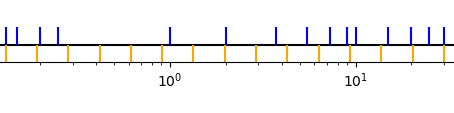
\includegraphics[width=0.4\linewidth]{Python/Lab_mes_points_zoom.png}
    \caption{Position of 15 hot wire measurement points on $y$ axis (log scale, millimetres). Given ones (blue superior lines) and equally distributed (lower orange lines) between $y_{min} = 0.13$ \si{mm} and $h = 30$ \si{mm}}
    \label{fig:mes_points}
\end{figure}

At these 15 points will be sampled time series data for PDF determination. Besides at 3 of these points are provided larger data measurements (at higher sampling frequencies) so that a spectrum can be computed with a sufficient resolution.\\

During the experiment, the channel fan is set to blow air at an approximate centre line velocity of $U_0 \sim 5$ \si{m/s} which correspond to a Reynolds number of $Re = U_0 D/\nu \sim \num{2e5}$. This is far above the threshold for a fully developed turbulence in a channel flow empirically located around $Re \sim 2900$. 


\subsection{Anemometer calibration}

Measurements of speed are obtained with hot-wire anemometry technique. It consists of a very thin wire that is immersed in a fluid flow. An electric current goes through the wire and heat it up (Joule's effect). The temperature reached depends on the thermal dissipation by the flow (with a conductive and convective part) so that at a given current, each flow speed leads to a determined wire temperature. The narrowness of the wire might let us assume that the wire temperature reaches its equilibrium at a given flow speed before speed flow actually changes (so that we don't have to deal with time variation of temperature in the wire). This should nonetheless give a frequency threshold for time scale of speed variations that are shorter than the time scale of wire temperature variation.\\

As a classical ohmic resistor, resistance of the wire changes with its temperature. Measuring resistance variation from its usual value provide a way of computing speed changes. For instance Wheatstone bridge is a common electrical circuit for obtaining the resistance value through a tension measurement. Nonetheless, this relation between flow speed and voltage has to be determined empirically since it depends of the room temperature, usual resistance, geometry and materials properties of the wire...\\

\begin{figure}[ht!]
    \centering
    \resizebox{0.6\linewidth}{!}{%% Creator: Matplotlib, PGF backend
%%
%% To include the figure in your LaTeX document, write
%%   \input{<filename>.pgf}
%%
%% Make sure the required packages are loaded in your preamble
%%   \usepackage{pgf}
%%
%% Figures using additional raster images can only be included by \input if
%% they are in the same directory as the main LaTeX file. For loading figures
%% from other directories you can use the `import` package
%%   \usepackage{import}
%% and then include the figures with
%%   \import{<path to file>}{<filename>.pgf}
%%
%% Matplotlib used the following preamble
%%
\begingroup%
\makeatletter%
\begin{pgfpicture}%
\pgfpathrectangle{\pgfpointorigin}{\pgfqpoint{6.400000in}{4.800000in}}%
\pgfusepath{use as bounding box, clip}%
\begin{pgfscope}%
\pgfsetbuttcap%
\pgfsetmiterjoin%
\definecolor{currentfill}{rgb}{1.000000,1.000000,1.000000}%
\pgfsetfillcolor{currentfill}%
\pgfsetlinewidth{0.000000pt}%
\definecolor{currentstroke}{rgb}{1.000000,1.000000,1.000000}%
\pgfsetstrokecolor{currentstroke}%
\pgfsetdash{}{0pt}%
\pgfpathmoveto{\pgfqpoint{0.000000in}{0.000000in}}%
\pgfpathlineto{\pgfqpoint{6.400000in}{0.000000in}}%
\pgfpathlineto{\pgfqpoint{6.400000in}{4.800000in}}%
\pgfpathlineto{\pgfqpoint{0.000000in}{4.800000in}}%
\pgfpathclose%
\pgfusepath{fill}%
\end{pgfscope}%
\begin{pgfscope}%
\pgfsetbuttcap%
\pgfsetmiterjoin%
\definecolor{currentfill}{rgb}{1.000000,1.000000,1.000000}%
\pgfsetfillcolor{currentfill}%
\pgfsetlinewidth{0.000000pt}%
\definecolor{currentstroke}{rgb}{0.000000,0.000000,0.000000}%
\pgfsetstrokecolor{currentstroke}%
\pgfsetstrokeopacity{0.000000}%
\pgfsetdash{}{0pt}%
\pgfpathmoveto{\pgfqpoint{0.800000in}{0.528000in}}%
\pgfpathlineto{\pgfqpoint{5.760000in}{0.528000in}}%
\pgfpathlineto{\pgfqpoint{5.760000in}{4.224000in}}%
\pgfpathlineto{\pgfqpoint{0.800000in}{4.224000in}}%
\pgfpathclose%
\pgfusepath{fill}%
\end{pgfscope}%
\begin{pgfscope}%
\pgfsetbuttcap%
\pgfsetroundjoin%
\definecolor{currentfill}{rgb}{0.000000,0.000000,0.000000}%
\pgfsetfillcolor{currentfill}%
\pgfsetlinewidth{0.803000pt}%
\definecolor{currentstroke}{rgb}{0.000000,0.000000,0.000000}%
\pgfsetstrokecolor{currentstroke}%
\pgfsetdash{}{0pt}%
\pgfsys@defobject{currentmarker}{\pgfqpoint{0.000000in}{-0.048611in}}{\pgfqpoint{0.000000in}{0.000000in}}{%
\pgfpathmoveto{\pgfqpoint{0.000000in}{0.000000in}}%
\pgfpathlineto{\pgfqpoint{0.000000in}{-0.048611in}}%
\pgfusepath{stroke,fill}%
}%
\begin{pgfscope}%
\pgfsys@transformshift{1.168327in}{0.528000in}%
\pgfsys@useobject{currentmarker}{}%
\end{pgfscope}%
\end{pgfscope}%
\begin{pgfscope}%
\definecolor{textcolor}{rgb}{0.000000,0.000000,0.000000}%
\pgfsetstrokecolor{textcolor}%
\pgfsetfillcolor{textcolor}%
\pgftext[x=1.168327in,y=0.430778in,,top]{\color{textcolor}\rmfamily\fontsize{10.000000}{12.000000}\selectfont \(\displaystyle 2.5\)}%
\end{pgfscope}%
\begin{pgfscope}%
\pgfsetbuttcap%
\pgfsetroundjoin%
\definecolor{currentfill}{rgb}{0.000000,0.000000,0.000000}%
\pgfsetfillcolor{currentfill}%
\pgfsetlinewidth{0.803000pt}%
\definecolor{currentstroke}{rgb}{0.000000,0.000000,0.000000}%
\pgfsetstrokecolor{currentstroke}%
\pgfsetdash{}{0pt}%
\pgfsys@defobject{currentmarker}{\pgfqpoint{0.000000in}{-0.048611in}}{\pgfqpoint{0.000000in}{0.000000in}}{%
\pgfpathmoveto{\pgfqpoint{0.000000in}{0.000000in}}%
\pgfpathlineto{\pgfqpoint{0.000000in}{-0.048611in}}%
\pgfusepath{stroke,fill}%
}%
\begin{pgfscope}%
\pgfsys@transformshift{1.766500in}{0.528000in}%
\pgfsys@useobject{currentmarker}{}%
\end{pgfscope}%
\end{pgfscope}%
\begin{pgfscope}%
\definecolor{textcolor}{rgb}{0.000000,0.000000,0.000000}%
\pgfsetstrokecolor{textcolor}%
\pgfsetfillcolor{textcolor}%
\pgftext[x=1.766500in,y=0.430778in,,top]{\color{textcolor}\rmfamily\fontsize{10.000000}{12.000000}\selectfont \(\displaystyle 5.0\)}%
\end{pgfscope}%
\begin{pgfscope}%
\pgfsetbuttcap%
\pgfsetroundjoin%
\definecolor{currentfill}{rgb}{0.000000,0.000000,0.000000}%
\pgfsetfillcolor{currentfill}%
\pgfsetlinewidth{0.803000pt}%
\definecolor{currentstroke}{rgb}{0.000000,0.000000,0.000000}%
\pgfsetstrokecolor{currentstroke}%
\pgfsetdash{}{0pt}%
\pgfsys@defobject{currentmarker}{\pgfqpoint{0.000000in}{-0.048611in}}{\pgfqpoint{0.000000in}{0.000000in}}{%
\pgfpathmoveto{\pgfqpoint{0.000000in}{0.000000in}}%
\pgfpathlineto{\pgfqpoint{0.000000in}{-0.048611in}}%
\pgfusepath{stroke,fill}%
}%
\begin{pgfscope}%
\pgfsys@transformshift{2.364673in}{0.528000in}%
\pgfsys@useobject{currentmarker}{}%
\end{pgfscope}%
\end{pgfscope}%
\begin{pgfscope}%
\definecolor{textcolor}{rgb}{0.000000,0.000000,0.000000}%
\pgfsetstrokecolor{textcolor}%
\pgfsetfillcolor{textcolor}%
\pgftext[x=2.364673in,y=0.430778in,,top]{\color{textcolor}\rmfamily\fontsize{10.000000}{12.000000}\selectfont \(\displaystyle 7.5\)}%
\end{pgfscope}%
\begin{pgfscope}%
\pgfsetbuttcap%
\pgfsetroundjoin%
\definecolor{currentfill}{rgb}{0.000000,0.000000,0.000000}%
\pgfsetfillcolor{currentfill}%
\pgfsetlinewidth{0.803000pt}%
\definecolor{currentstroke}{rgb}{0.000000,0.000000,0.000000}%
\pgfsetstrokecolor{currentstroke}%
\pgfsetdash{}{0pt}%
\pgfsys@defobject{currentmarker}{\pgfqpoint{0.000000in}{-0.048611in}}{\pgfqpoint{0.000000in}{0.000000in}}{%
\pgfpathmoveto{\pgfqpoint{0.000000in}{0.000000in}}%
\pgfpathlineto{\pgfqpoint{0.000000in}{-0.048611in}}%
\pgfusepath{stroke,fill}%
}%
\begin{pgfscope}%
\pgfsys@transformshift{2.962846in}{0.528000in}%
\pgfsys@useobject{currentmarker}{}%
\end{pgfscope}%
\end{pgfscope}%
\begin{pgfscope}%
\definecolor{textcolor}{rgb}{0.000000,0.000000,0.000000}%
\pgfsetstrokecolor{textcolor}%
\pgfsetfillcolor{textcolor}%
\pgftext[x=2.962846in,y=0.430778in,,top]{\color{textcolor}\rmfamily\fontsize{10.000000}{12.000000}\selectfont \(\displaystyle 10.0\)}%
\end{pgfscope}%
\begin{pgfscope}%
\pgfsetbuttcap%
\pgfsetroundjoin%
\definecolor{currentfill}{rgb}{0.000000,0.000000,0.000000}%
\pgfsetfillcolor{currentfill}%
\pgfsetlinewidth{0.803000pt}%
\definecolor{currentstroke}{rgb}{0.000000,0.000000,0.000000}%
\pgfsetstrokecolor{currentstroke}%
\pgfsetdash{}{0pt}%
\pgfsys@defobject{currentmarker}{\pgfqpoint{0.000000in}{-0.048611in}}{\pgfqpoint{0.000000in}{0.000000in}}{%
\pgfpathmoveto{\pgfqpoint{0.000000in}{0.000000in}}%
\pgfpathlineto{\pgfqpoint{0.000000in}{-0.048611in}}%
\pgfusepath{stroke,fill}%
}%
\begin{pgfscope}%
\pgfsys@transformshift{3.561019in}{0.528000in}%
\pgfsys@useobject{currentmarker}{}%
\end{pgfscope}%
\end{pgfscope}%
\begin{pgfscope}%
\definecolor{textcolor}{rgb}{0.000000,0.000000,0.000000}%
\pgfsetstrokecolor{textcolor}%
\pgfsetfillcolor{textcolor}%
\pgftext[x=3.561019in,y=0.430778in,,top]{\color{textcolor}\rmfamily\fontsize{10.000000}{12.000000}\selectfont \(\displaystyle 12.5\)}%
\end{pgfscope}%
\begin{pgfscope}%
\pgfsetbuttcap%
\pgfsetroundjoin%
\definecolor{currentfill}{rgb}{0.000000,0.000000,0.000000}%
\pgfsetfillcolor{currentfill}%
\pgfsetlinewidth{0.803000pt}%
\definecolor{currentstroke}{rgb}{0.000000,0.000000,0.000000}%
\pgfsetstrokecolor{currentstroke}%
\pgfsetdash{}{0pt}%
\pgfsys@defobject{currentmarker}{\pgfqpoint{0.000000in}{-0.048611in}}{\pgfqpoint{0.000000in}{0.000000in}}{%
\pgfpathmoveto{\pgfqpoint{0.000000in}{0.000000in}}%
\pgfpathlineto{\pgfqpoint{0.000000in}{-0.048611in}}%
\pgfusepath{stroke,fill}%
}%
\begin{pgfscope}%
\pgfsys@transformshift{4.159192in}{0.528000in}%
\pgfsys@useobject{currentmarker}{}%
\end{pgfscope}%
\end{pgfscope}%
\begin{pgfscope}%
\definecolor{textcolor}{rgb}{0.000000,0.000000,0.000000}%
\pgfsetstrokecolor{textcolor}%
\pgfsetfillcolor{textcolor}%
\pgftext[x=4.159192in,y=0.430778in,,top]{\color{textcolor}\rmfamily\fontsize{10.000000}{12.000000}\selectfont \(\displaystyle 15.0\)}%
\end{pgfscope}%
\begin{pgfscope}%
\pgfsetbuttcap%
\pgfsetroundjoin%
\definecolor{currentfill}{rgb}{0.000000,0.000000,0.000000}%
\pgfsetfillcolor{currentfill}%
\pgfsetlinewidth{0.803000pt}%
\definecolor{currentstroke}{rgb}{0.000000,0.000000,0.000000}%
\pgfsetstrokecolor{currentstroke}%
\pgfsetdash{}{0pt}%
\pgfsys@defobject{currentmarker}{\pgfqpoint{0.000000in}{-0.048611in}}{\pgfqpoint{0.000000in}{0.000000in}}{%
\pgfpathmoveto{\pgfqpoint{0.000000in}{0.000000in}}%
\pgfpathlineto{\pgfqpoint{0.000000in}{-0.048611in}}%
\pgfusepath{stroke,fill}%
}%
\begin{pgfscope}%
\pgfsys@transformshift{4.757365in}{0.528000in}%
\pgfsys@useobject{currentmarker}{}%
\end{pgfscope}%
\end{pgfscope}%
\begin{pgfscope}%
\definecolor{textcolor}{rgb}{0.000000,0.000000,0.000000}%
\pgfsetstrokecolor{textcolor}%
\pgfsetfillcolor{textcolor}%
\pgftext[x=4.757365in,y=0.430778in,,top]{\color{textcolor}\rmfamily\fontsize{10.000000}{12.000000}\selectfont \(\displaystyle 17.5\)}%
\end{pgfscope}%
\begin{pgfscope}%
\pgfsetbuttcap%
\pgfsetroundjoin%
\definecolor{currentfill}{rgb}{0.000000,0.000000,0.000000}%
\pgfsetfillcolor{currentfill}%
\pgfsetlinewidth{0.803000pt}%
\definecolor{currentstroke}{rgb}{0.000000,0.000000,0.000000}%
\pgfsetstrokecolor{currentstroke}%
\pgfsetdash{}{0pt}%
\pgfsys@defobject{currentmarker}{\pgfqpoint{0.000000in}{-0.048611in}}{\pgfqpoint{0.000000in}{0.000000in}}{%
\pgfpathmoveto{\pgfqpoint{0.000000in}{0.000000in}}%
\pgfpathlineto{\pgfqpoint{0.000000in}{-0.048611in}}%
\pgfusepath{stroke,fill}%
}%
\begin{pgfscope}%
\pgfsys@transformshift{5.355539in}{0.528000in}%
\pgfsys@useobject{currentmarker}{}%
\end{pgfscope}%
\end{pgfscope}%
\begin{pgfscope}%
\definecolor{textcolor}{rgb}{0.000000,0.000000,0.000000}%
\pgfsetstrokecolor{textcolor}%
\pgfsetfillcolor{textcolor}%
\pgftext[x=5.355539in,y=0.430778in,,top]{\color{textcolor}\rmfamily\fontsize{10.000000}{12.000000}\selectfont \(\displaystyle 20.0\)}%
\end{pgfscope}%
\begin{pgfscope}%
\definecolor{textcolor}{rgb}{0.000000,0.000000,0.000000}%
\pgfsetstrokecolor{textcolor}%
\pgfsetfillcolor{textcolor}%
\pgftext[x=3.280000in,y=0.251766in,,top]{\color{textcolor}\rmfamily\fontsize{10.000000}{12.000000}\selectfont Velocity \(\displaystyle U\)}%
\end{pgfscope}%
\begin{pgfscope}%
\pgfsetbuttcap%
\pgfsetroundjoin%
\definecolor{currentfill}{rgb}{0.000000,0.000000,0.000000}%
\pgfsetfillcolor{currentfill}%
\pgfsetlinewidth{0.803000pt}%
\definecolor{currentstroke}{rgb}{0.000000,0.000000,0.000000}%
\pgfsetstrokecolor{currentstroke}%
\pgfsetdash{}{0pt}%
\pgfsys@defobject{currentmarker}{\pgfqpoint{-0.048611in}{0.000000in}}{\pgfqpoint{0.000000in}{0.000000in}}{%
\pgfpathmoveto{\pgfqpoint{0.000000in}{0.000000in}}%
\pgfpathlineto{\pgfqpoint{-0.048611in}{0.000000in}}%
\pgfusepath{stroke,fill}%
}%
\begin{pgfscope}%
\pgfsys@transformshift{0.800000in}{1.014674in}%
\pgfsys@useobject{currentmarker}{}%
\end{pgfscope}%
\end{pgfscope}%
\begin{pgfscope}%
\definecolor{textcolor}{rgb}{0.000000,0.000000,0.000000}%
\pgfsetstrokecolor{textcolor}%
\pgfsetfillcolor{textcolor}%
\pgftext[x=0.525308in,y=0.966448in,left,base]{\color{textcolor}\rmfamily\fontsize{10.000000}{12.000000}\selectfont \(\displaystyle 1.2\)}%
\end{pgfscope}%
\begin{pgfscope}%
\pgfsetbuttcap%
\pgfsetroundjoin%
\definecolor{currentfill}{rgb}{0.000000,0.000000,0.000000}%
\pgfsetfillcolor{currentfill}%
\pgfsetlinewidth{0.803000pt}%
\definecolor{currentstroke}{rgb}{0.000000,0.000000,0.000000}%
\pgfsetstrokecolor{currentstroke}%
\pgfsetdash{}{0pt}%
\pgfsys@defobject{currentmarker}{\pgfqpoint{-0.048611in}{0.000000in}}{\pgfqpoint{0.000000in}{0.000000in}}{%
\pgfpathmoveto{\pgfqpoint{0.000000in}{0.000000in}}%
\pgfpathlineto{\pgfqpoint{-0.048611in}{0.000000in}}%
\pgfusepath{stroke,fill}%
}%
\begin{pgfscope}%
\pgfsys@transformshift{0.800000in}{1.579440in}%
\pgfsys@useobject{currentmarker}{}%
\end{pgfscope}%
\end{pgfscope}%
\begin{pgfscope}%
\definecolor{textcolor}{rgb}{0.000000,0.000000,0.000000}%
\pgfsetstrokecolor{textcolor}%
\pgfsetfillcolor{textcolor}%
\pgftext[x=0.525308in,y=1.531215in,left,base]{\color{textcolor}\rmfamily\fontsize{10.000000}{12.000000}\selectfont \(\displaystyle 1.3\)}%
\end{pgfscope}%
\begin{pgfscope}%
\pgfsetbuttcap%
\pgfsetroundjoin%
\definecolor{currentfill}{rgb}{0.000000,0.000000,0.000000}%
\pgfsetfillcolor{currentfill}%
\pgfsetlinewidth{0.803000pt}%
\definecolor{currentstroke}{rgb}{0.000000,0.000000,0.000000}%
\pgfsetstrokecolor{currentstroke}%
\pgfsetdash{}{0pt}%
\pgfsys@defobject{currentmarker}{\pgfqpoint{-0.048611in}{0.000000in}}{\pgfqpoint{0.000000in}{0.000000in}}{%
\pgfpathmoveto{\pgfqpoint{0.000000in}{0.000000in}}%
\pgfpathlineto{\pgfqpoint{-0.048611in}{0.000000in}}%
\pgfusepath{stroke,fill}%
}%
\begin{pgfscope}%
\pgfsys@transformshift{0.800000in}{2.144207in}%
\pgfsys@useobject{currentmarker}{}%
\end{pgfscope}%
\end{pgfscope}%
\begin{pgfscope}%
\definecolor{textcolor}{rgb}{0.000000,0.000000,0.000000}%
\pgfsetstrokecolor{textcolor}%
\pgfsetfillcolor{textcolor}%
\pgftext[x=0.525308in,y=2.095982in,left,base]{\color{textcolor}\rmfamily\fontsize{10.000000}{12.000000}\selectfont \(\displaystyle 1.4\)}%
\end{pgfscope}%
\begin{pgfscope}%
\pgfsetbuttcap%
\pgfsetroundjoin%
\definecolor{currentfill}{rgb}{0.000000,0.000000,0.000000}%
\pgfsetfillcolor{currentfill}%
\pgfsetlinewidth{0.803000pt}%
\definecolor{currentstroke}{rgb}{0.000000,0.000000,0.000000}%
\pgfsetstrokecolor{currentstroke}%
\pgfsetdash{}{0pt}%
\pgfsys@defobject{currentmarker}{\pgfqpoint{-0.048611in}{0.000000in}}{\pgfqpoint{0.000000in}{0.000000in}}{%
\pgfpathmoveto{\pgfqpoint{0.000000in}{0.000000in}}%
\pgfpathlineto{\pgfqpoint{-0.048611in}{0.000000in}}%
\pgfusepath{stroke,fill}%
}%
\begin{pgfscope}%
\pgfsys@transformshift{0.800000in}{2.708974in}%
\pgfsys@useobject{currentmarker}{}%
\end{pgfscope}%
\end{pgfscope}%
\begin{pgfscope}%
\definecolor{textcolor}{rgb}{0.000000,0.000000,0.000000}%
\pgfsetstrokecolor{textcolor}%
\pgfsetfillcolor{textcolor}%
\pgftext[x=0.525308in,y=2.660749in,left,base]{\color{textcolor}\rmfamily\fontsize{10.000000}{12.000000}\selectfont \(\displaystyle 1.5\)}%
\end{pgfscope}%
\begin{pgfscope}%
\pgfsetbuttcap%
\pgfsetroundjoin%
\definecolor{currentfill}{rgb}{0.000000,0.000000,0.000000}%
\pgfsetfillcolor{currentfill}%
\pgfsetlinewidth{0.803000pt}%
\definecolor{currentstroke}{rgb}{0.000000,0.000000,0.000000}%
\pgfsetstrokecolor{currentstroke}%
\pgfsetdash{}{0pt}%
\pgfsys@defobject{currentmarker}{\pgfqpoint{-0.048611in}{0.000000in}}{\pgfqpoint{0.000000in}{0.000000in}}{%
\pgfpathmoveto{\pgfqpoint{0.000000in}{0.000000in}}%
\pgfpathlineto{\pgfqpoint{-0.048611in}{0.000000in}}%
\pgfusepath{stroke,fill}%
}%
\begin{pgfscope}%
\pgfsys@transformshift{0.800000in}{3.273741in}%
\pgfsys@useobject{currentmarker}{}%
\end{pgfscope}%
\end{pgfscope}%
\begin{pgfscope}%
\definecolor{textcolor}{rgb}{0.000000,0.000000,0.000000}%
\pgfsetstrokecolor{textcolor}%
\pgfsetfillcolor{textcolor}%
\pgftext[x=0.525308in,y=3.225516in,left,base]{\color{textcolor}\rmfamily\fontsize{10.000000}{12.000000}\selectfont \(\displaystyle 1.6\)}%
\end{pgfscope}%
\begin{pgfscope}%
\pgfsetbuttcap%
\pgfsetroundjoin%
\definecolor{currentfill}{rgb}{0.000000,0.000000,0.000000}%
\pgfsetfillcolor{currentfill}%
\pgfsetlinewidth{0.803000pt}%
\definecolor{currentstroke}{rgb}{0.000000,0.000000,0.000000}%
\pgfsetstrokecolor{currentstroke}%
\pgfsetdash{}{0pt}%
\pgfsys@defobject{currentmarker}{\pgfqpoint{-0.048611in}{0.000000in}}{\pgfqpoint{0.000000in}{0.000000in}}{%
\pgfpathmoveto{\pgfqpoint{0.000000in}{0.000000in}}%
\pgfpathlineto{\pgfqpoint{-0.048611in}{0.000000in}}%
\pgfusepath{stroke,fill}%
}%
\begin{pgfscope}%
\pgfsys@transformshift{0.800000in}{3.838508in}%
\pgfsys@useobject{currentmarker}{}%
\end{pgfscope}%
\end{pgfscope}%
\begin{pgfscope}%
\definecolor{textcolor}{rgb}{0.000000,0.000000,0.000000}%
\pgfsetstrokecolor{textcolor}%
\pgfsetfillcolor{textcolor}%
\pgftext[x=0.525308in,y=3.790283in,left,base]{\color{textcolor}\rmfamily\fontsize{10.000000}{12.000000}\selectfont \(\displaystyle 1.7\)}%
\end{pgfscope}%
\begin{pgfscope}%
\definecolor{textcolor}{rgb}{0.000000,0.000000,0.000000}%
\pgfsetstrokecolor{textcolor}%
\pgfsetfillcolor{textcolor}%
\pgftext[x=0.469752in,y=2.376000in,,bottom,rotate=90.000000]{\color{textcolor}\rmfamily\fontsize{10.000000}{12.000000}\selectfont Square output voltage \(\displaystyle E^2\)}%
\end{pgfscope}%
\begin{pgfscope}%
\pgfpathrectangle{\pgfqpoint{0.800000in}{0.528000in}}{\pgfqpoint{4.960000in}{3.696000in}}%
\pgfusepath{clip}%
\pgfsetbuttcap%
\pgfsetmiterjoin%
\definecolor{currentfill}{rgb}{0.121569,0.466667,0.705882}%
\pgfsetfillcolor{currentfill}%
\pgfsetlinewidth{1.003750pt}%
\definecolor{currentstroke}{rgb}{0.121569,0.466667,0.705882}%
\pgfsetstrokecolor{currentstroke}%
\pgfsetdash{}{0pt}%
\pgfsys@defobject{currentmarker}{\pgfqpoint{-0.041667in}{-0.041667in}}{\pgfqpoint{0.041667in}{0.041667in}}{%
\pgfpathmoveto{\pgfqpoint{-0.041667in}{-0.041667in}}%
\pgfpathlineto{\pgfqpoint{0.041667in}{-0.041667in}}%
\pgfpathlineto{\pgfqpoint{0.041667in}{0.041667in}}%
\pgfpathlineto{\pgfqpoint{-0.041667in}{0.041667in}}%
\pgfpathclose%
\pgfusepath{stroke,fill}%
}%
\begin{pgfscope}%
\pgfsys@transformshift{1.025455in}{0.706537in}%
\pgfsys@useobject{currentmarker}{}%
\end{pgfscope}%
\begin{pgfscope}%
\pgfsys@transformshift{1.116162in}{0.844227in}%
\pgfsys@useobject{currentmarker}{}%
\end{pgfscope}%
\begin{pgfscope}%
\pgfsys@transformshift{1.193742in}{0.956390in}%
\pgfsys@useobject{currentmarker}{}%
\end{pgfscope}%
\begin{pgfscope}%
\pgfsys@transformshift{1.333916in}{1.142876in}%
\pgfsys@useobject{currentmarker}{}%
\end{pgfscope}%
\begin{pgfscope}%
\pgfsys@transformshift{1.451433in}{1.286383in}%
\pgfsys@useobject{currentmarker}{}%
\end{pgfscope}%
\begin{pgfscope}%
\pgfsys@transformshift{1.568167in}{1.421362in}%
\pgfsys@useobject{currentmarker}{}%
\end{pgfscope}%
\begin{pgfscope}%
\pgfsys@transformshift{1.639439in}{1.500599in}%
\pgfsys@useobject{currentmarker}{}%
\end{pgfscope}%
\begin{pgfscope}%
\pgfsys@transformshift{1.742207in}{1.609260in}%
\pgfsys@useobject{currentmarker}{}%
\end{pgfscope}%
\begin{pgfscope}%
\pgfsys@transformshift{1.820259in}{1.688610in}%
\pgfsys@useobject{currentmarker}{}%
\end{pgfscope}%
\begin{pgfscope}%
\pgfsys@transformshift{1.892270in}{1.760505in}%
\pgfsys@useobject{currentmarker}{}%
\end{pgfscope}%
\begin{pgfscope}%
\pgfsys@transformshift{1.964766in}{1.828390in}%
\pgfsys@useobject{currentmarker}{}%
\end{pgfscope}%
\begin{pgfscope}%
\pgfsys@transformshift{2.096706in}{1.949419in}%
\pgfsys@useobject{currentmarker}{}%
\end{pgfscope}%
\begin{pgfscope}%
\pgfsys@transformshift{2.221932in}{2.058645in}%
\pgfsys@useobject{currentmarker}{}%
\end{pgfscope}%
\begin{pgfscope}%
\pgfsys@transformshift{2.330003in}{2.149799in}%
\pgfsys@useobject{currentmarker}{}%
\end{pgfscope}%
\begin{pgfscope}%
\pgfsys@transformshift{2.442864in}{2.239710in}%
\pgfsys@useobject{currentmarker}{}%
\end{pgfscope}%
\begin{pgfscope}%
\pgfsys@transformshift{2.542673in}{2.318495in}%
\pgfsys@useobject{currentmarker}{}%
\end{pgfscope}%
\begin{pgfscope}%
\pgfsys@transformshift{2.769696in}{2.487473in}%
\pgfsys@useobject{currentmarker}{}%
\end{pgfscope}%
\begin{pgfscope}%
\pgfsys@transformshift{2.984402in}{2.638717in}%
\pgfsys@useobject{currentmarker}{}%
\end{pgfscope}%
\begin{pgfscope}%
\pgfsys@transformshift{3.346955in}{2.877840in}%
\pgfsys@useobject{currentmarker}{}%
\end{pgfscope}%
\begin{pgfscope}%
\pgfsys@transformshift{3.677527in}{3.080083in}%
\pgfsys@useobject{currentmarker}{}%
\end{pgfscope}%
\begin{pgfscope}%
\pgfsys@transformshift{3.961470in}{3.244656in}%
\pgfsys@useobject{currentmarker}{}%
\end{pgfscope}%
\begin{pgfscope}%
\pgfsys@transformshift{4.232459in}{3.397595in}%
\pgfsys@useobject{currentmarker}{}%
\end{pgfscope}%
\begin{pgfscope}%
\pgfsys@transformshift{4.489913in}{3.534212in}%
\pgfsys@useobject{currentmarker}{}%
\end{pgfscope}%
\begin{pgfscope}%
\pgfsys@transformshift{4.712684in}{3.650497in}%
\pgfsys@useobject{currentmarker}{}%
\end{pgfscope}%
\begin{pgfscope}%
\pgfsys@transformshift{4.951839in}{3.770171in}%
\pgfsys@useobject{currentmarker}{}%
\end{pgfscope}%
\begin{pgfscope}%
\pgfsys@transformshift{5.141232in}{3.869006in}%
\pgfsys@useobject{currentmarker}{}%
\end{pgfscope}%
\begin{pgfscope}%
\pgfsys@transformshift{5.340917in}{3.965807in}%
\pgfsys@useobject{currentmarker}{}%
\end{pgfscope}%
\begin{pgfscope}%
\pgfsys@transformshift{5.534545in}{4.056000in}%
\pgfsys@useobject{currentmarker}{}%
\end{pgfscope}%
\end{pgfscope}%
\begin{pgfscope}%
\pgfpathrectangle{\pgfqpoint{0.800000in}{0.528000in}}{\pgfqpoint{4.960000in}{3.696000in}}%
\pgfusepath{clip}%
\pgfsetrectcap%
\pgfsetroundjoin%
\pgfsetlinewidth{1.505625pt}%
\definecolor{currentstroke}{rgb}{1.000000,0.498039,0.054902}%
\pgfsetstrokecolor{currentstroke}%
\pgfsetdash{}{0pt}%
\pgfpathmoveto{\pgfqpoint{1.025455in}{0.696000in}}%
\pgfpathlineto{\pgfqpoint{1.075104in}{0.778088in}}%
\pgfpathlineto{\pgfqpoint{1.124754in}{0.855906in}}%
\pgfpathlineto{\pgfqpoint{1.178917in}{0.936603in}}%
\pgfpathlineto{\pgfqpoint{1.237594in}{1.019746in}}%
\pgfpathlineto{\pgfqpoint{1.296271in}{1.099013in}}%
\pgfpathlineto{\pgfqpoint{1.359461in}{1.180584in}}%
\pgfpathlineto{\pgfqpoint{1.427165in}{1.264143in}}%
\pgfpathlineto{\pgfqpoint{1.494869in}{1.344194in}}%
\pgfpathlineto{\pgfqpoint{1.567087in}{1.426152in}}%
\pgfpathlineto{\pgfqpoint{1.643818in}{1.509779in}}%
\pgfpathlineto{\pgfqpoint{1.725063in}{1.594865in}}%
\pgfpathlineto{\pgfqpoint{1.806308in}{1.676764in}}%
\pgfpathlineto{\pgfqpoint{1.892067in}{1.760105in}}%
\pgfpathlineto{\pgfqpoint{1.982339in}{1.844724in}}%
\pgfpathlineto{\pgfqpoint{2.077124in}{1.930474in}}%
\pgfpathlineto{\pgfqpoint{2.176424in}{2.017226in}}%
\pgfpathlineto{\pgfqpoint{2.280237in}{2.104866in}}%
\pgfpathlineto{\pgfqpoint{2.388563in}{2.193294in}}%
\pgfpathlineto{\pgfqpoint{2.501403in}{2.282419in}}%
\pgfpathlineto{\pgfqpoint{2.618757in}{2.372162in}}%
\pgfpathlineto{\pgfqpoint{2.740624in}{2.462454in}}%
\pgfpathlineto{\pgfqpoint{2.867005in}{2.553232in}}%
\pgfpathlineto{\pgfqpoint{2.997900in}{2.644441in}}%
\pgfpathlineto{\pgfqpoint{3.133308in}{2.736031in}}%
\pgfpathlineto{\pgfqpoint{3.273230in}{2.827958in}}%
\pgfpathlineto{\pgfqpoint{3.417665in}{2.920183in}}%
\pgfpathlineto{\pgfqpoint{3.566614in}{3.012671in}}%
\pgfpathlineto{\pgfqpoint{3.720076in}{3.105390in}}%
\pgfpathlineto{\pgfqpoint{3.882566in}{3.200931in}}%
\pgfpathlineto{\pgfqpoint{4.049570in}{3.296514in}}%
\pgfpathlineto{\pgfqpoint{4.221087in}{3.392126in}}%
\pgfpathlineto{\pgfqpoint{4.401631in}{3.490174in}}%
\pgfpathlineto{\pgfqpoint{4.586689in}{3.588107in}}%
\pgfpathlineto{\pgfqpoint{4.776260in}{3.685924in}}%
\pgfpathlineto{\pgfqpoint{4.974858in}{3.785869in}}%
\pgfpathlineto{\pgfqpoint{5.177971in}{3.885589in}}%
\pgfpathlineto{\pgfqpoint{5.390110in}{3.987228in}}%
\pgfpathlineto{\pgfqpoint{5.534545in}{4.055048in}}%
\pgfpathlineto{\pgfqpoint{5.534545in}{4.055048in}}%
\pgfusepath{stroke}%
\end{pgfscope}%
\begin{pgfscope}%
\pgfsetrectcap%
\pgfsetmiterjoin%
\pgfsetlinewidth{0.803000pt}%
\definecolor{currentstroke}{rgb}{0.000000,0.000000,0.000000}%
\pgfsetstrokecolor{currentstroke}%
\pgfsetdash{}{0pt}%
\pgfpathmoveto{\pgfqpoint{0.800000in}{0.528000in}}%
\pgfpathlineto{\pgfqpoint{0.800000in}{4.224000in}}%
\pgfusepath{stroke}%
\end{pgfscope}%
\begin{pgfscope}%
\pgfsetrectcap%
\pgfsetmiterjoin%
\pgfsetlinewidth{0.803000pt}%
\definecolor{currentstroke}{rgb}{0.000000,0.000000,0.000000}%
\pgfsetstrokecolor{currentstroke}%
\pgfsetdash{}{0pt}%
\pgfpathmoveto{\pgfqpoint{5.760000in}{0.528000in}}%
\pgfpathlineto{\pgfqpoint{5.760000in}{4.224000in}}%
\pgfusepath{stroke}%
\end{pgfscope}%
\begin{pgfscope}%
\pgfsetrectcap%
\pgfsetmiterjoin%
\pgfsetlinewidth{0.803000pt}%
\definecolor{currentstroke}{rgb}{0.000000,0.000000,0.000000}%
\pgfsetstrokecolor{currentstroke}%
\pgfsetdash{}{0pt}%
\pgfpathmoveto{\pgfqpoint{0.800000in}{0.528000in}}%
\pgfpathlineto{\pgfqpoint{5.760000in}{0.528000in}}%
\pgfusepath{stroke}%
\end{pgfscope}%
\begin{pgfscope}%
\pgfsetrectcap%
\pgfsetmiterjoin%
\pgfsetlinewidth{0.803000pt}%
\definecolor{currentstroke}{rgb}{0.000000,0.000000,0.000000}%
\pgfsetstrokecolor{currentstroke}%
\pgfsetdash{}{0pt}%
\pgfpathmoveto{\pgfqpoint{0.800000in}{4.224000in}}%
\pgfpathlineto{\pgfqpoint{5.760000in}{4.224000in}}%
\pgfusepath{stroke}%
\end{pgfscope}%
\begin{pgfscope}%
\pgfsetbuttcap%
\pgfsetmiterjoin%
\definecolor{currentfill}{rgb}{1.000000,1.000000,1.000000}%
\pgfsetfillcolor{currentfill}%
\pgfsetfillopacity{0.800000}%
\pgfsetlinewidth{1.003750pt}%
\definecolor{currentstroke}{rgb}{0.800000,0.800000,0.800000}%
\pgfsetstrokecolor{currentstroke}%
\pgfsetstrokeopacity{0.800000}%
\pgfsetdash{}{0pt}%
\pgfpathmoveto{\pgfqpoint{0.897222in}{3.725543in}}%
\pgfpathlineto{\pgfqpoint{2.722071in}{3.725543in}}%
\pgfpathquadraticcurveto{\pgfqpoint{2.749849in}{3.725543in}}{\pgfqpoint{2.749849in}{3.753321in}}%
\pgfpathlineto{\pgfqpoint{2.749849in}{4.126778in}}%
\pgfpathquadraticcurveto{\pgfqpoint{2.749849in}{4.154556in}}{\pgfqpoint{2.722071in}{4.154556in}}%
\pgfpathlineto{\pgfqpoint{0.897222in}{4.154556in}}%
\pgfpathquadraticcurveto{\pgfqpoint{0.869444in}{4.154556in}}{\pgfqpoint{0.869444in}{4.126778in}}%
\pgfpathlineto{\pgfqpoint{0.869444in}{3.753321in}}%
\pgfpathquadraticcurveto{\pgfqpoint{0.869444in}{3.725543in}}{\pgfqpoint{0.897222in}{3.725543in}}%
\pgfpathclose%
\pgfusepath{stroke,fill}%
\end{pgfscope}%
\begin{pgfscope}%
\pgfsetbuttcap%
\pgfsetmiterjoin%
\definecolor{currentfill}{rgb}{0.121569,0.466667,0.705882}%
\pgfsetfillcolor{currentfill}%
\pgfsetlinewidth{1.003750pt}%
\definecolor{currentstroke}{rgb}{0.121569,0.466667,0.705882}%
\pgfsetstrokecolor{currentstroke}%
\pgfsetdash{}{0pt}%
\pgfsys@defobject{currentmarker}{\pgfqpoint{-0.041667in}{-0.041667in}}{\pgfqpoint{0.041667in}{0.041667in}}{%
\pgfpathmoveto{\pgfqpoint{-0.041667in}{-0.041667in}}%
\pgfpathlineto{\pgfqpoint{0.041667in}{-0.041667in}}%
\pgfpathlineto{\pgfqpoint{0.041667in}{0.041667in}}%
\pgfpathlineto{\pgfqpoint{-0.041667in}{0.041667in}}%
\pgfpathclose%
\pgfusepath{stroke,fill}%
}%
\begin{pgfscope}%
\pgfsys@transformshift{1.063889in}{4.050389in}%
\pgfsys@useobject{currentmarker}{}%
\end{pgfscope}%
\end{pgfscope}%
\begin{pgfscope}%
\definecolor{textcolor}{rgb}{0.000000,0.000000,0.000000}%
\pgfsetstrokecolor{textcolor}%
\pgfsetfillcolor{textcolor}%
\pgftext[x=1.313889in,y=4.001778in,left,base]{\color{textcolor}\rmfamily\fontsize{10.000000}{12.000000}\selectfont Provided data}%
\end{pgfscope}%
\begin{pgfscope}%
\pgfsetrectcap%
\pgfsetroundjoin%
\pgfsetlinewidth{1.505625pt}%
\definecolor{currentstroke}{rgb}{1.000000,0.498039,0.054902}%
\pgfsetstrokecolor{currentstroke}%
\pgfsetdash{}{0pt}%
\pgfpathmoveto{\pgfqpoint{0.925000in}{3.856716in}}%
\pgfpathlineto{\pgfqpoint{1.202778in}{3.856716in}}%
\pgfusepath{stroke}%
\end{pgfscope}%
\begin{pgfscope}%
\definecolor{textcolor}{rgb}{0.000000,0.000000,0.000000}%
\pgfsetstrokecolor{textcolor}%
\pgfsetfillcolor{textcolor}%
\pgftext[x=1.313889in,y=3.808105in,left,base]{\color{textcolor}\rmfamily\fontsize{10.000000}{12.000000}\selectfont King's Law calibration}%
\end{pgfscope}%
\end{pgfpicture}%
\makeatother%
\endgroup%
}
    \caption{Calibration of King's Law coefficients $A = \num{8.44e-1}$ \si{V^2}, $B = \num{2.23e-1}$ \si{uSI} and $n=0.458$ with a L2-normalized residual rms $e_{rms} = \num{4.6e-4}$}
    \label{fig:AnemometerFitting}
\end{figure}

This calibration is achieved with the calibration which results are presented on figure \ref{fig:AnemometerFitting} and obtained with \verb|Python|'s file \verb|CalibrationAnemometer.py|. It consists of a minimization process in $\mathbb{R}^3$ of parameters $A,B$ and $n$. For a set of data $y \in \mathbb{R}^p$, we minimize the following quantity : \\ 

\begin{equation}
    \min_{(A,B,n)\in\mathbb{R}^3} \frac{\sqrt{\frac{1}{p} \sum_{y} \left( E^2(y) - A - BU^n(y) \right)^2 }}{\sqrt{ \frac{1}{p} \sum \left( E^2\right)^2}}
\end{equation}



%% Rappeler les valeurs dans un tableau synthétoqie et expliquer l'expression de l'erreur e_rms

\newpage
\section{Results}

In figure \ref{fig:Mean_Velocity_Profile} we represent the mean velocity profile in a log-lin scale with a fitting of the log-law performed on the central points. More precisely, the excluded points are the two first (sorted by $y$) since they visually are out of the region where most of the points seems aligned.  Moreover I chose not to take into account the four last points for the log-law fitting because their are located quite far beyond the empirical threshold $\eta = 0.3$. \\

At this point there is no numerical value for the threshold $y^+=30$ yet because we need $u_*$ to compute $y^+$. And one way of determining $u_*$ is using the log-law fitting. $u_*$ could also have been determined using the linear law in the very near region to the wall where $u^+ = y^+$ with a linear fitting of slope $\alpha$ and $u_* = \sqrt{\nu\alpha}$ but the imprecision is too high at this stage. Indeed the method using the log-law fitting gives $u_* = \num{2.30e-1} \si{m/s}$ while a fitting with the two first points of the linear law gives $u_* = \num{1.53e-2} \si{m/s}$.\\

The root-mean-square profile of average-free speed $u_{RMS}$ is plotted at figure \ref{fig:RMS_Profile} and the skewness $S_u$ is depicted at figure \ref{fig:Skewness_Profile} with :\\

\begin{align}
    u_{RMS} &= \sqrt{<\left(\tilde{u}-\bar{U}\right)^2>} \\
    S_u &= \frac{<\left(\tilde{u}-\bar{U}\right)^3>}{u_{RMS}^3}
\end{align}

The probability density function (PDF) for the three locations is presented at figure \ref{fig:PDF}.b. It is obtained by a custom written function which is avalaible in the github repository. The PDF is obtained from the reconstruction of the CDF which is quite easy, following the method explained in algorithm \ref{algo:PDF}. It can be noted that steps 4 and 5 could be done in the inverse order. The filtering at step 5 uses the scientific \verb|Python| library \verb|scipy| with the zero-phase filtering function \verb|filtfilt| configured with a 3\up{rd}-order butterworth low-pass filter with hand-tuned frequency cut.\\

\begin{algorithm}
\label{algo:PDF}
\caption{PDF calculation}
\SetAlgoLined
\KwResult{Return vectors $u_{PDF}$ and $PDF_u$}
\textbf{Step 1} : get time series data $u$\;
Sort in ascending order $u \rightarrow u_{sorted}$\;
\textbf{Step 2} : Computing the CDF\;
\For{$k = 0$ to length of $u_{sorted}$}{
delete duplications of $u_{sorted}$'s values \;
\If{$u_{sorted}[k] > u_{sorted}[k-1]$}{
$u_{sorted}[k]$ is appended to $u_{PDF}$\;
Relative position in sorted data $k/\textnormal{length}(u_{sorted})$ is appended to $CDF_u$\;
}
}
\textbf{Step 3} : Interpolation of CDF on a regular range of $u_{CDF}$ to ease derivation and filtering\;
\textbf{Step 4} : Derivation of CDF with respect to $u_{CDF} \rightarrow  PDF_u^{noisy}$\;
\textbf{Step 5} : Denoising of PDF with a low-pass filter\;
\end{algorithm}


\begin{figure}
    \centering
        \resizebox{0.6\linewidth}{!}{%% Creator: Matplotlib, PGF backend
%%
%% To include the figure in your LaTeX document, write
%%   \input{<filename>.pgf}
%%
%% Make sure the required packages are loaded in your preamble
%%   \usepackage{pgf}
%%
%% Figures using additional raster images can only be included by \input if
%% they are in the same directory as the main LaTeX file. For loading figures
%% from other directories you can use the `import` package
%%   \usepackage{import}
%% and then include the figures with
%%   \import{<path to file>}{<filename>.pgf}
%%
%% Matplotlib used the following preamble
%%   \usepackage{fontspec}
%%   \setmainfont{DejaVuSerif.ttf}[Path=C:/Users/garaya/AppData/Local/Continuum/anaconda3/lib/site-packages/matplotlib/mpl-data/fonts/ttf/]
%%   \setsansfont{DejaVuSans.ttf}[Path=C:/Users/garaya/AppData/Local/Continuum/anaconda3/lib/site-packages/matplotlib/mpl-data/fonts/ttf/]
%%   \setmonofont{DejaVuSansMono.ttf}[Path=C:/Users/garaya/AppData/Local/Continuum/anaconda3/lib/site-packages/matplotlib/mpl-data/fonts/ttf/]
%%
\begingroup%
\makeatletter%
\begin{pgfpicture}%
\pgfpathrectangle{\pgfpointorigin}{\pgfqpoint{6.400000in}{4.780000in}}%
\pgfusepath{use as bounding box, clip}%
\begin{pgfscope}%
\pgfsetbuttcap%
\pgfsetmiterjoin%
\definecolor{currentfill}{rgb}{1.000000,1.000000,1.000000}%
\pgfsetfillcolor{currentfill}%
\pgfsetlinewidth{0.000000pt}%
\definecolor{currentstroke}{rgb}{1.000000,1.000000,1.000000}%
\pgfsetstrokecolor{currentstroke}%
\pgfsetdash{}{0pt}%
\pgfpathmoveto{\pgfqpoint{0.000000in}{0.000000in}}%
\pgfpathlineto{\pgfqpoint{6.400000in}{0.000000in}}%
\pgfpathlineto{\pgfqpoint{6.400000in}{4.780000in}}%
\pgfpathlineto{\pgfqpoint{0.000000in}{4.780000in}}%
\pgfpathclose%
\pgfusepath{fill}%
\end{pgfscope}%
\begin{pgfscope}%
\pgfsetbuttcap%
\pgfsetmiterjoin%
\definecolor{currentfill}{rgb}{1.000000,1.000000,1.000000}%
\pgfsetfillcolor{currentfill}%
\pgfsetlinewidth{0.000000pt}%
\definecolor{currentstroke}{rgb}{0.000000,0.000000,0.000000}%
\pgfsetstrokecolor{currentstroke}%
\pgfsetstrokeopacity{0.000000}%
\pgfsetdash{}{0pt}%
\pgfpathmoveto{\pgfqpoint{0.798865in}{0.725653in}}%
\pgfpathlineto{\pgfqpoint{6.190000in}{0.725653in}}%
\pgfpathlineto{\pgfqpoint{6.190000in}{4.570875in}}%
\pgfpathlineto{\pgfqpoint{0.798865in}{4.570875in}}%
\pgfpathclose%
\pgfusepath{fill}%
\end{pgfscope}%
\begin{pgfscope}%
\pgfsetbuttcap%
\pgfsetroundjoin%
\definecolor{currentfill}{rgb}{0.000000,0.000000,0.000000}%
\pgfsetfillcolor{currentfill}%
\pgfsetlinewidth{0.803000pt}%
\definecolor{currentstroke}{rgb}{0.000000,0.000000,0.000000}%
\pgfsetstrokecolor{currentstroke}%
\pgfsetdash{}{0pt}%
\pgfsys@defobject{currentmarker}{\pgfqpoint{0.000000in}{-0.048611in}}{\pgfqpoint{0.000000in}{0.000000in}}{%
\pgfpathmoveto{\pgfqpoint{0.000000in}{0.000000in}}%
\pgfpathlineto{\pgfqpoint{0.000000in}{-0.048611in}}%
\pgfusepath{stroke,fill}%
}%
\begin{pgfscope}%
\pgfsys@transformshift{1.962835in}{0.725653in}%
\pgfsys@useobject{currentmarker}{}%
\end{pgfscope}%
\end{pgfscope}%
\begin{pgfscope}%
\definecolor{textcolor}{rgb}{0.000000,0.000000,0.000000}%
\pgfsetstrokecolor{textcolor}%
\pgfsetfillcolor{textcolor}%
\pgftext[x=1.962835in,y=0.628430in,,top]{\color{textcolor}\rmfamily\fontsize{14.000000}{16.800000}\selectfont \(\displaystyle 10^{-2}\)}%
\end{pgfscope}%
\begin{pgfscope}%
\pgfsetbuttcap%
\pgfsetroundjoin%
\definecolor{currentfill}{rgb}{0.000000,0.000000,0.000000}%
\pgfsetfillcolor{currentfill}%
\pgfsetlinewidth{0.803000pt}%
\definecolor{currentstroke}{rgb}{0.000000,0.000000,0.000000}%
\pgfsetstrokecolor{currentstroke}%
\pgfsetdash{}{0pt}%
\pgfsys@defobject{currentmarker}{\pgfqpoint{0.000000in}{-0.048611in}}{\pgfqpoint{0.000000in}{0.000000in}}{%
\pgfpathmoveto{\pgfqpoint{0.000000in}{0.000000in}}%
\pgfpathlineto{\pgfqpoint{0.000000in}{-0.048611in}}%
\pgfusepath{stroke,fill}%
}%
\begin{pgfscope}%
\pgfsys@transformshift{3.953892in}{0.725653in}%
\pgfsys@useobject{currentmarker}{}%
\end{pgfscope}%
\end{pgfscope}%
\begin{pgfscope}%
\definecolor{textcolor}{rgb}{0.000000,0.000000,0.000000}%
\pgfsetstrokecolor{textcolor}%
\pgfsetfillcolor{textcolor}%
\pgftext[x=3.953892in,y=0.628430in,,top]{\color{textcolor}\rmfamily\fontsize{14.000000}{16.800000}\selectfont \(\displaystyle 10^{-1}\)}%
\end{pgfscope}%
\begin{pgfscope}%
\pgfsetbuttcap%
\pgfsetroundjoin%
\definecolor{currentfill}{rgb}{0.000000,0.000000,0.000000}%
\pgfsetfillcolor{currentfill}%
\pgfsetlinewidth{0.803000pt}%
\definecolor{currentstroke}{rgb}{0.000000,0.000000,0.000000}%
\pgfsetstrokecolor{currentstroke}%
\pgfsetdash{}{0pt}%
\pgfsys@defobject{currentmarker}{\pgfqpoint{0.000000in}{-0.048611in}}{\pgfqpoint{0.000000in}{0.000000in}}{%
\pgfpathmoveto{\pgfqpoint{0.000000in}{0.000000in}}%
\pgfpathlineto{\pgfqpoint{0.000000in}{-0.048611in}}%
\pgfusepath{stroke,fill}%
}%
\begin{pgfscope}%
\pgfsys@transformshift{5.944948in}{0.725653in}%
\pgfsys@useobject{currentmarker}{}%
\end{pgfscope}%
\end{pgfscope}%
\begin{pgfscope}%
\definecolor{textcolor}{rgb}{0.000000,0.000000,0.000000}%
\pgfsetstrokecolor{textcolor}%
\pgfsetfillcolor{textcolor}%
\pgftext[x=5.944948in,y=0.628430in,,top]{\color{textcolor}\rmfamily\fontsize{14.000000}{16.800000}\selectfont \(\displaystyle 10^{0}\)}%
\end{pgfscope}%
\begin{pgfscope}%
\pgfsetbuttcap%
\pgfsetroundjoin%
\definecolor{currentfill}{rgb}{0.000000,0.000000,0.000000}%
\pgfsetfillcolor{currentfill}%
\pgfsetlinewidth{0.602250pt}%
\definecolor{currentstroke}{rgb}{0.000000,0.000000,0.000000}%
\pgfsetstrokecolor{currentstroke}%
\pgfsetdash{}{0pt}%
\pgfsys@defobject{currentmarker}{\pgfqpoint{0.000000in}{-0.027778in}}{\pgfqpoint{0.000000in}{0.000000in}}{%
\pgfpathmoveto{\pgfqpoint{0.000000in}{0.000000in}}%
\pgfpathlineto{\pgfqpoint{0.000000in}{-0.027778in}}%
\pgfusepath{stroke,fill}%
}%
\begin{pgfscope}%
\pgfsys@transformshift{0.921754in}{0.725653in}%
\pgfsys@useobject{currentmarker}{}%
\end{pgfscope}%
\end{pgfscope}%
\begin{pgfscope}%
\pgfsetbuttcap%
\pgfsetroundjoin%
\definecolor{currentfill}{rgb}{0.000000,0.000000,0.000000}%
\pgfsetfillcolor{currentfill}%
\pgfsetlinewidth{0.602250pt}%
\definecolor{currentstroke}{rgb}{0.000000,0.000000,0.000000}%
\pgfsetstrokecolor{currentstroke}%
\pgfsetdash{}{0pt}%
\pgfsys@defobject{currentmarker}{\pgfqpoint{0.000000in}{-0.027778in}}{\pgfqpoint{0.000000in}{0.000000in}}{%
\pgfpathmoveto{\pgfqpoint{0.000000in}{0.000000in}}%
\pgfpathlineto{\pgfqpoint{0.000000in}{-0.027778in}}%
\pgfusepath{stroke,fill}%
}%
\begin{pgfscope}%
\pgfsys@transformshift{1.170514in}{0.725653in}%
\pgfsys@useobject{currentmarker}{}%
\end{pgfscope}%
\end{pgfscope}%
\begin{pgfscope}%
\pgfsetbuttcap%
\pgfsetroundjoin%
\definecolor{currentfill}{rgb}{0.000000,0.000000,0.000000}%
\pgfsetfillcolor{currentfill}%
\pgfsetlinewidth{0.602250pt}%
\definecolor{currentstroke}{rgb}{0.000000,0.000000,0.000000}%
\pgfsetstrokecolor{currentstroke}%
\pgfsetdash{}{0pt}%
\pgfsys@defobject{currentmarker}{\pgfqpoint{0.000000in}{-0.027778in}}{\pgfqpoint{0.000000in}{0.000000in}}{%
\pgfpathmoveto{\pgfqpoint{0.000000in}{0.000000in}}%
\pgfpathlineto{\pgfqpoint{0.000000in}{-0.027778in}}%
\pgfusepath{stroke,fill}%
}%
\begin{pgfscope}%
\pgfsys@transformshift{1.363467in}{0.725653in}%
\pgfsys@useobject{currentmarker}{}%
\end{pgfscope}%
\end{pgfscope}%
\begin{pgfscope}%
\pgfsetbuttcap%
\pgfsetroundjoin%
\definecolor{currentfill}{rgb}{0.000000,0.000000,0.000000}%
\pgfsetfillcolor{currentfill}%
\pgfsetlinewidth{0.602250pt}%
\definecolor{currentstroke}{rgb}{0.000000,0.000000,0.000000}%
\pgfsetstrokecolor{currentstroke}%
\pgfsetdash{}{0pt}%
\pgfsys@defobject{currentmarker}{\pgfqpoint{0.000000in}{-0.027778in}}{\pgfqpoint{0.000000in}{0.000000in}}{%
\pgfpathmoveto{\pgfqpoint{0.000000in}{0.000000in}}%
\pgfpathlineto{\pgfqpoint{0.000000in}{-0.027778in}}%
\pgfusepath{stroke,fill}%
}%
\begin{pgfscope}%
\pgfsys@transformshift{1.521122in}{0.725653in}%
\pgfsys@useobject{currentmarker}{}%
\end{pgfscope}%
\end{pgfscope}%
\begin{pgfscope}%
\pgfsetbuttcap%
\pgfsetroundjoin%
\definecolor{currentfill}{rgb}{0.000000,0.000000,0.000000}%
\pgfsetfillcolor{currentfill}%
\pgfsetlinewidth{0.602250pt}%
\definecolor{currentstroke}{rgb}{0.000000,0.000000,0.000000}%
\pgfsetstrokecolor{currentstroke}%
\pgfsetdash{}{0pt}%
\pgfsys@defobject{currentmarker}{\pgfqpoint{0.000000in}{-0.027778in}}{\pgfqpoint{0.000000in}{0.000000in}}{%
\pgfpathmoveto{\pgfqpoint{0.000000in}{0.000000in}}%
\pgfpathlineto{\pgfqpoint{0.000000in}{-0.027778in}}%
\pgfusepath{stroke,fill}%
}%
\begin{pgfscope}%
\pgfsys@transformshift{1.654417in}{0.725653in}%
\pgfsys@useobject{currentmarker}{}%
\end{pgfscope}%
\end{pgfscope}%
\begin{pgfscope}%
\pgfsetbuttcap%
\pgfsetroundjoin%
\definecolor{currentfill}{rgb}{0.000000,0.000000,0.000000}%
\pgfsetfillcolor{currentfill}%
\pgfsetlinewidth{0.602250pt}%
\definecolor{currentstroke}{rgb}{0.000000,0.000000,0.000000}%
\pgfsetstrokecolor{currentstroke}%
\pgfsetdash{}{0pt}%
\pgfsys@defobject{currentmarker}{\pgfqpoint{0.000000in}{-0.027778in}}{\pgfqpoint{0.000000in}{0.000000in}}{%
\pgfpathmoveto{\pgfqpoint{0.000000in}{0.000000in}}%
\pgfpathlineto{\pgfqpoint{0.000000in}{-0.027778in}}%
\pgfusepath{stroke,fill}%
}%
\begin{pgfscope}%
\pgfsys@transformshift{1.769882in}{0.725653in}%
\pgfsys@useobject{currentmarker}{}%
\end{pgfscope}%
\end{pgfscope}%
\begin{pgfscope}%
\pgfsetbuttcap%
\pgfsetroundjoin%
\definecolor{currentfill}{rgb}{0.000000,0.000000,0.000000}%
\pgfsetfillcolor{currentfill}%
\pgfsetlinewidth{0.602250pt}%
\definecolor{currentstroke}{rgb}{0.000000,0.000000,0.000000}%
\pgfsetstrokecolor{currentstroke}%
\pgfsetdash{}{0pt}%
\pgfsys@defobject{currentmarker}{\pgfqpoint{0.000000in}{-0.027778in}}{\pgfqpoint{0.000000in}{0.000000in}}{%
\pgfpathmoveto{\pgfqpoint{0.000000in}{0.000000in}}%
\pgfpathlineto{\pgfqpoint{0.000000in}{-0.027778in}}%
\pgfusepath{stroke,fill}%
}%
\begin{pgfscope}%
\pgfsys@transformshift{1.871729in}{0.725653in}%
\pgfsys@useobject{currentmarker}{}%
\end{pgfscope}%
\end{pgfscope}%
\begin{pgfscope}%
\pgfsetbuttcap%
\pgfsetroundjoin%
\definecolor{currentfill}{rgb}{0.000000,0.000000,0.000000}%
\pgfsetfillcolor{currentfill}%
\pgfsetlinewidth{0.602250pt}%
\definecolor{currentstroke}{rgb}{0.000000,0.000000,0.000000}%
\pgfsetstrokecolor{currentstroke}%
\pgfsetdash{}{0pt}%
\pgfsys@defobject{currentmarker}{\pgfqpoint{0.000000in}{-0.027778in}}{\pgfqpoint{0.000000in}{0.000000in}}{%
\pgfpathmoveto{\pgfqpoint{0.000000in}{0.000000in}}%
\pgfpathlineto{\pgfqpoint{0.000000in}{-0.027778in}}%
\pgfusepath{stroke,fill}%
}%
\begin{pgfscope}%
\pgfsys@transformshift{2.562203in}{0.725653in}%
\pgfsys@useobject{currentmarker}{}%
\end{pgfscope}%
\end{pgfscope}%
\begin{pgfscope}%
\pgfsetbuttcap%
\pgfsetroundjoin%
\definecolor{currentfill}{rgb}{0.000000,0.000000,0.000000}%
\pgfsetfillcolor{currentfill}%
\pgfsetlinewidth{0.602250pt}%
\definecolor{currentstroke}{rgb}{0.000000,0.000000,0.000000}%
\pgfsetstrokecolor{currentstroke}%
\pgfsetdash{}{0pt}%
\pgfsys@defobject{currentmarker}{\pgfqpoint{0.000000in}{-0.027778in}}{\pgfqpoint{0.000000in}{0.000000in}}{%
\pgfpathmoveto{\pgfqpoint{0.000000in}{0.000000in}}%
\pgfpathlineto{\pgfqpoint{0.000000in}{-0.027778in}}%
\pgfusepath{stroke,fill}%
}%
\begin{pgfscope}%
\pgfsys@transformshift{2.912811in}{0.725653in}%
\pgfsys@useobject{currentmarker}{}%
\end{pgfscope}%
\end{pgfscope}%
\begin{pgfscope}%
\pgfsetbuttcap%
\pgfsetroundjoin%
\definecolor{currentfill}{rgb}{0.000000,0.000000,0.000000}%
\pgfsetfillcolor{currentfill}%
\pgfsetlinewidth{0.602250pt}%
\definecolor{currentstroke}{rgb}{0.000000,0.000000,0.000000}%
\pgfsetstrokecolor{currentstroke}%
\pgfsetdash{}{0pt}%
\pgfsys@defobject{currentmarker}{\pgfqpoint{0.000000in}{-0.027778in}}{\pgfqpoint{0.000000in}{0.000000in}}{%
\pgfpathmoveto{\pgfqpoint{0.000000in}{0.000000in}}%
\pgfpathlineto{\pgfqpoint{0.000000in}{-0.027778in}}%
\pgfusepath{stroke,fill}%
}%
\begin{pgfscope}%
\pgfsys@transformshift{3.161571in}{0.725653in}%
\pgfsys@useobject{currentmarker}{}%
\end{pgfscope}%
\end{pgfscope}%
\begin{pgfscope}%
\pgfsetbuttcap%
\pgfsetroundjoin%
\definecolor{currentfill}{rgb}{0.000000,0.000000,0.000000}%
\pgfsetfillcolor{currentfill}%
\pgfsetlinewidth{0.602250pt}%
\definecolor{currentstroke}{rgb}{0.000000,0.000000,0.000000}%
\pgfsetstrokecolor{currentstroke}%
\pgfsetdash{}{0pt}%
\pgfsys@defobject{currentmarker}{\pgfqpoint{0.000000in}{-0.027778in}}{\pgfqpoint{0.000000in}{0.000000in}}{%
\pgfpathmoveto{\pgfqpoint{0.000000in}{0.000000in}}%
\pgfpathlineto{\pgfqpoint{0.000000in}{-0.027778in}}%
\pgfusepath{stroke,fill}%
}%
\begin{pgfscope}%
\pgfsys@transformshift{3.354524in}{0.725653in}%
\pgfsys@useobject{currentmarker}{}%
\end{pgfscope}%
\end{pgfscope}%
\begin{pgfscope}%
\pgfsetbuttcap%
\pgfsetroundjoin%
\definecolor{currentfill}{rgb}{0.000000,0.000000,0.000000}%
\pgfsetfillcolor{currentfill}%
\pgfsetlinewidth{0.602250pt}%
\definecolor{currentstroke}{rgb}{0.000000,0.000000,0.000000}%
\pgfsetstrokecolor{currentstroke}%
\pgfsetdash{}{0pt}%
\pgfsys@defobject{currentmarker}{\pgfqpoint{0.000000in}{-0.027778in}}{\pgfqpoint{0.000000in}{0.000000in}}{%
\pgfpathmoveto{\pgfqpoint{0.000000in}{0.000000in}}%
\pgfpathlineto{\pgfqpoint{0.000000in}{-0.027778in}}%
\pgfusepath{stroke,fill}%
}%
\begin{pgfscope}%
\pgfsys@transformshift{3.512178in}{0.725653in}%
\pgfsys@useobject{currentmarker}{}%
\end{pgfscope}%
\end{pgfscope}%
\begin{pgfscope}%
\pgfsetbuttcap%
\pgfsetroundjoin%
\definecolor{currentfill}{rgb}{0.000000,0.000000,0.000000}%
\pgfsetfillcolor{currentfill}%
\pgfsetlinewidth{0.602250pt}%
\definecolor{currentstroke}{rgb}{0.000000,0.000000,0.000000}%
\pgfsetstrokecolor{currentstroke}%
\pgfsetdash{}{0pt}%
\pgfsys@defobject{currentmarker}{\pgfqpoint{0.000000in}{-0.027778in}}{\pgfqpoint{0.000000in}{0.000000in}}{%
\pgfpathmoveto{\pgfqpoint{0.000000in}{0.000000in}}%
\pgfpathlineto{\pgfqpoint{0.000000in}{-0.027778in}}%
\pgfusepath{stroke,fill}%
}%
\begin{pgfscope}%
\pgfsys@transformshift{3.645473in}{0.725653in}%
\pgfsys@useobject{currentmarker}{}%
\end{pgfscope}%
\end{pgfscope}%
\begin{pgfscope}%
\pgfsetbuttcap%
\pgfsetroundjoin%
\definecolor{currentfill}{rgb}{0.000000,0.000000,0.000000}%
\pgfsetfillcolor{currentfill}%
\pgfsetlinewidth{0.602250pt}%
\definecolor{currentstroke}{rgb}{0.000000,0.000000,0.000000}%
\pgfsetstrokecolor{currentstroke}%
\pgfsetdash{}{0pt}%
\pgfsys@defobject{currentmarker}{\pgfqpoint{0.000000in}{-0.027778in}}{\pgfqpoint{0.000000in}{0.000000in}}{%
\pgfpathmoveto{\pgfqpoint{0.000000in}{0.000000in}}%
\pgfpathlineto{\pgfqpoint{0.000000in}{-0.027778in}}%
\pgfusepath{stroke,fill}%
}%
\begin{pgfscope}%
\pgfsys@transformshift{3.760938in}{0.725653in}%
\pgfsys@useobject{currentmarker}{}%
\end{pgfscope}%
\end{pgfscope}%
\begin{pgfscope}%
\pgfsetbuttcap%
\pgfsetroundjoin%
\definecolor{currentfill}{rgb}{0.000000,0.000000,0.000000}%
\pgfsetfillcolor{currentfill}%
\pgfsetlinewidth{0.602250pt}%
\definecolor{currentstroke}{rgb}{0.000000,0.000000,0.000000}%
\pgfsetstrokecolor{currentstroke}%
\pgfsetdash{}{0pt}%
\pgfsys@defobject{currentmarker}{\pgfqpoint{0.000000in}{-0.027778in}}{\pgfqpoint{0.000000in}{0.000000in}}{%
\pgfpathmoveto{\pgfqpoint{0.000000in}{0.000000in}}%
\pgfpathlineto{\pgfqpoint{0.000000in}{-0.027778in}}%
\pgfusepath{stroke,fill}%
}%
\begin{pgfscope}%
\pgfsys@transformshift{3.862786in}{0.725653in}%
\pgfsys@useobject{currentmarker}{}%
\end{pgfscope}%
\end{pgfscope}%
\begin{pgfscope}%
\pgfsetbuttcap%
\pgfsetroundjoin%
\definecolor{currentfill}{rgb}{0.000000,0.000000,0.000000}%
\pgfsetfillcolor{currentfill}%
\pgfsetlinewidth{0.602250pt}%
\definecolor{currentstroke}{rgb}{0.000000,0.000000,0.000000}%
\pgfsetstrokecolor{currentstroke}%
\pgfsetdash{}{0pt}%
\pgfsys@defobject{currentmarker}{\pgfqpoint{0.000000in}{-0.027778in}}{\pgfqpoint{0.000000in}{0.000000in}}{%
\pgfpathmoveto{\pgfqpoint{0.000000in}{0.000000in}}%
\pgfpathlineto{\pgfqpoint{0.000000in}{-0.027778in}}%
\pgfusepath{stroke,fill}%
}%
\begin{pgfscope}%
\pgfsys@transformshift{4.553260in}{0.725653in}%
\pgfsys@useobject{currentmarker}{}%
\end{pgfscope}%
\end{pgfscope}%
\begin{pgfscope}%
\pgfsetbuttcap%
\pgfsetroundjoin%
\definecolor{currentfill}{rgb}{0.000000,0.000000,0.000000}%
\pgfsetfillcolor{currentfill}%
\pgfsetlinewidth{0.602250pt}%
\definecolor{currentstroke}{rgb}{0.000000,0.000000,0.000000}%
\pgfsetstrokecolor{currentstroke}%
\pgfsetdash{}{0pt}%
\pgfsys@defobject{currentmarker}{\pgfqpoint{0.000000in}{-0.027778in}}{\pgfqpoint{0.000000in}{0.000000in}}{%
\pgfpathmoveto{\pgfqpoint{0.000000in}{0.000000in}}%
\pgfpathlineto{\pgfqpoint{0.000000in}{-0.027778in}}%
\pgfusepath{stroke,fill}%
}%
\begin{pgfscope}%
\pgfsys@transformshift{4.903867in}{0.725653in}%
\pgfsys@useobject{currentmarker}{}%
\end{pgfscope}%
\end{pgfscope}%
\begin{pgfscope}%
\pgfsetbuttcap%
\pgfsetroundjoin%
\definecolor{currentfill}{rgb}{0.000000,0.000000,0.000000}%
\pgfsetfillcolor{currentfill}%
\pgfsetlinewidth{0.602250pt}%
\definecolor{currentstroke}{rgb}{0.000000,0.000000,0.000000}%
\pgfsetstrokecolor{currentstroke}%
\pgfsetdash{}{0pt}%
\pgfsys@defobject{currentmarker}{\pgfqpoint{0.000000in}{-0.027778in}}{\pgfqpoint{0.000000in}{0.000000in}}{%
\pgfpathmoveto{\pgfqpoint{0.000000in}{0.000000in}}%
\pgfpathlineto{\pgfqpoint{0.000000in}{-0.027778in}}%
\pgfusepath{stroke,fill}%
}%
\begin{pgfscope}%
\pgfsys@transformshift{5.152627in}{0.725653in}%
\pgfsys@useobject{currentmarker}{}%
\end{pgfscope}%
\end{pgfscope}%
\begin{pgfscope}%
\pgfsetbuttcap%
\pgfsetroundjoin%
\definecolor{currentfill}{rgb}{0.000000,0.000000,0.000000}%
\pgfsetfillcolor{currentfill}%
\pgfsetlinewidth{0.602250pt}%
\definecolor{currentstroke}{rgb}{0.000000,0.000000,0.000000}%
\pgfsetstrokecolor{currentstroke}%
\pgfsetdash{}{0pt}%
\pgfsys@defobject{currentmarker}{\pgfqpoint{0.000000in}{-0.027778in}}{\pgfqpoint{0.000000in}{0.000000in}}{%
\pgfpathmoveto{\pgfqpoint{0.000000in}{0.000000in}}%
\pgfpathlineto{\pgfqpoint{0.000000in}{-0.027778in}}%
\pgfusepath{stroke,fill}%
}%
\begin{pgfscope}%
\pgfsys@transformshift{5.345581in}{0.725653in}%
\pgfsys@useobject{currentmarker}{}%
\end{pgfscope}%
\end{pgfscope}%
\begin{pgfscope}%
\pgfsetbuttcap%
\pgfsetroundjoin%
\definecolor{currentfill}{rgb}{0.000000,0.000000,0.000000}%
\pgfsetfillcolor{currentfill}%
\pgfsetlinewidth{0.602250pt}%
\definecolor{currentstroke}{rgb}{0.000000,0.000000,0.000000}%
\pgfsetstrokecolor{currentstroke}%
\pgfsetdash{}{0pt}%
\pgfsys@defobject{currentmarker}{\pgfqpoint{0.000000in}{-0.027778in}}{\pgfqpoint{0.000000in}{0.000000in}}{%
\pgfpathmoveto{\pgfqpoint{0.000000in}{0.000000in}}%
\pgfpathlineto{\pgfqpoint{0.000000in}{-0.027778in}}%
\pgfusepath{stroke,fill}%
}%
\begin{pgfscope}%
\pgfsys@transformshift{5.503235in}{0.725653in}%
\pgfsys@useobject{currentmarker}{}%
\end{pgfscope}%
\end{pgfscope}%
\begin{pgfscope}%
\pgfsetbuttcap%
\pgfsetroundjoin%
\definecolor{currentfill}{rgb}{0.000000,0.000000,0.000000}%
\pgfsetfillcolor{currentfill}%
\pgfsetlinewidth{0.602250pt}%
\definecolor{currentstroke}{rgb}{0.000000,0.000000,0.000000}%
\pgfsetstrokecolor{currentstroke}%
\pgfsetdash{}{0pt}%
\pgfsys@defobject{currentmarker}{\pgfqpoint{0.000000in}{-0.027778in}}{\pgfqpoint{0.000000in}{0.000000in}}{%
\pgfpathmoveto{\pgfqpoint{0.000000in}{0.000000in}}%
\pgfpathlineto{\pgfqpoint{0.000000in}{-0.027778in}}%
\pgfusepath{stroke,fill}%
}%
\begin{pgfscope}%
\pgfsys@transformshift{5.636530in}{0.725653in}%
\pgfsys@useobject{currentmarker}{}%
\end{pgfscope}%
\end{pgfscope}%
\begin{pgfscope}%
\pgfsetbuttcap%
\pgfsetroundjoin%
\definecolor{currentfill}{rgb}{0.000000,0.000000,0.000000}%
\pgfsetfillcolor{currentfill}%
\pgfsetlinewidth{0.602250pt}%
\definecolor{currentstroke}{rgb}{0.000000,0.000000,0.000000}%
\pgfsetstrokecolor{currentstroke}%
\pgfsetdash{}{0pt}%
\pgfsys@defobject{currentmarker}{\pgfqpoint{0.000000in}{-0.027778in}}{\pgfqpoint{0.000000in}{0.000000in}}{%
\pgfpathmoveto{\pgfqpoint{0.000000in}{0.000000in}}%
\pgfpathlineto{\pgfqpoint{0.000000in}{-0.027778in}}%
\pgfusepath{stroke,fill}%
}%
\begin{pgfscope}%
\pgfsys@transformshift{5.751995in}{0.725653in}%
\pgfsys@useobject{currentmarker}{}%
\end{pgfscope}%
\end{pgfscope}%
\begin{pgfscope}%
\pgfsetbuttcap%
\pgfsetroundjoin%
\definecolor{currentfill}{rgb}{0.000000,0.000000,0.000000}%
\pgfsetfillcolor{currentfill}%
\pgfsetlinewidth{0.602250pt}%
\definecolor{currentstroke}{rgb}{0.000000,0.000000,0.000000}%
\pgfsetstrokecolor{currentstroke}%
\pgfsetdash{}{0pt}%
\pgfsys@defobject{currentmarker}{\pgfqpoint{0.000000in}{-0.027778in}}{\pgfqpoint{0.000000in}{0.000000in}}{%
\pgfpathmoveto{\pgfqpoint{0.000000in}{0.000000in}}%
\pgfpathlineto{\pgfqpoint{0.000000in}{-0.027778in}}%
\pgfusepath{stroke,fill}%
}%
\begin{pgfscope}%
\pgfsys@transformshift{5.853843in}{0.725653in}%
\pgfsys@useobject{currentmarker}{}%
\end{pgfscope}%
\end{pgfscope}%
\begin{pgfscope}%
\definecolor{textcolor}{rgb}{0.000000,0.000000,0.000000}%
\pgfsetstrokecolor{textcolor}%
\pgfsetfillcolor{textcolor}%
\pgftext[x=3.494432in,y=0.384697in,,top]{\color{textcolor}\rmfamily\fontsize{14.000000}{16.800000}\selectfont Distance from wall \(\displaystyle \eta = y/h\) - log scale}%
\end{pgfscope}%
\begin{pgfscope}%
\pgfsetbuttcap%
\pgfsetroundjoin%
\definecolor{currentfill}{rgb}{0.000000,0.000000,0.000000}%
\pgfsetfillcolor{currentfill}%
\pgfsetlinewidth{0.803000pt}%
\definecolor{currentstroke}{rgb}{0.000000,0.000000,0.000000}%
\pgfsetstrokecolor{currentstroke}%
\pgfsetdash{}{0pt}%
\pgfsys@defobject{currentmarker}{\pgfqpoint{-0.048611in}{0.000000in}}{\pgfqpoint{0.000000in}{0.000000in}}{%
\pgfpathmoveto{\pgfqpoint{0.000000in}{0.000000in}}%
\pgfpathlineto{\pgfqpoint{-0.048611in}{0.000000in}}%
\pgfusepath{stroke,fill}%
}%
\begin{pgfscope}%
\pgfsys@transformshift{0.798865in}{0.815849in}%
\pgfsys@useobject{currentmarker}{}%
\end{pgfscope}%
\end{pgfscope}%
\begin{pgfscope}%
\definecolor{textcolor}{rgb}{0.000000,0.000000,0.000000}%
\pgfsetstrokecolor{textcolor}%
\pgfsetfillcolor{textcolor}%
\pgftext[x=0.451415in,y=0.741983in,left,base]{\color{textcolor}\rmfamily\fontsize{14.000000}{16.800000}\selectfont \(\displaystyle 2.0\)}%
\end{pgfscope}%
\begin{pgfscope}%
\pgfsetbuttcap%
\pgfsetroundjoin%
\definecolor{currentfill}{rgb}{0.000000,0.000000,0.000000}%
\pgfsetfillcolor{currentfill}%
\pgfsetlinewidth{0.803000pt}%
\definecolor{currentstroke}{rgb}{0.000000,0.000000,0.000000}%
\pgfsetstrokecolor{currentstroke}%
\pgfsetdash{}{0pt}%
\pgfsys@defobject{currentmarker}{\pgfqpoint{-0.048611in}{0.000000in}}{\pgfqpoint{0.000000in}{0.000000in}}{%
\pgfpathmoveto{\pgfqpoint{0.000000in}{0.000000in}}%
\pgfpathlineto{\pgfqpoint{-0.048611in}{0.000000in}}%
\pgfusepath{stroke,fill}%
}%
\begin{pgfscope}%
\pgfsys@transformshift{0.798865in}{1.369946in}%
\pgfsys@useobject{currentmarker}{}%
\end{pgfscope}%
\end{pgfscope}%
\begin{pgfscope}%
\definecolor{textcolor}{rgb}{0.000000,0.000000,0.000000}%
\pgfsetstrokecolor{textcolor}%
\pgfsetfillcolor{textcolor}%
\pgftext[x=0.451415in,y=1.296080in,left,base]{\color{textcolor}\rmfamily\fontsize{14.000000}{16.800000}\selectfont \(\displaystyle 2.5\)}%
\end{pgfscope}%
\begin{pgfscope}%
\pgfsetbuttcap%
\pgfsetroundjoin%
\definecolor{currentfill}{rgb}{0.000000,0.000000,0.000000}%
\pgfsetfillcolor{currentfill}%
\pgfsetlinewidth{0.803000pt}%
\definecolor{currentstroke}{rgb}{0.000000,0.000000,0.000000}%
\pgfsetstrokecolor{currentstroke}%
\pgfsetdash{}{0pt}%
\pgfsys@defobject{currentmarker}{\pgfqpoint{-0.048611in}{0.000000in}}{\pgfqpoint{0.000000in}{0.000000in}}{%
\pgfpathmoveto{\pgfqpoint{0.000000in}{0.000000in}}%
\pgfpathlineto{\pgfqpoint{-0.048611in}{0.000000in}}%
\pgfusepath{stroke,fill}%
}%
\begin{pgfscope}%
\pgfsys@transformshift{0.798865in}{1.924043in}%
\pgfsys@useobject{currentmarker}{}%
\end{pgfscope}%
\end{pgfscope}%
\begin{pgfscope}%
\definecolor{textcolor}{rgb}{0.000000,0.000000,0.000000}%
\pgfsetstrokecolor{textcolor}%
\pgfsetfillcolor{textcolor}%
\pgftext[x=0.451415in,y=1.850177in,left,base]{\color{textcolor}\rmfamily\fontsize{14.000000}{16.800000}\selectfont \(\displaystyle 3.0\)}%
\end{pgfscope}%
\begin{pgfscope}%
\pgfsetbuttcap%
\pgfsetroundjoin%
\definecolor{currentfill}{rgb}{0.000000,0.000000,0.000000}%
\pgfsetfillcolor{currentfill}%
\pgfsetlinewidth{0.803000pt}%
\definecolor{currentstroke}{rgb}{0.000000,0.000000,0.000000}%
\pgfsetstrokecolor{currentstroke}%
\pgfsetdash{}{0pt}%
\pgfsys@defobject{currentmarker}{\pgfqpoint{-0.048611in}{0.000000in}}{\pgfqpoint{0.000000in}{0.000000in}}{%
\pgfpathmoveto{\pgfqpoint{0.000000in}{0.000000in}}%
\pgfpathlineto{\pgfqpoint{-0.048611in}{0.000000in}}%
\pgfusepath{stroke,fill}%
}%
\begin{pgfscope}%
\pgfsys@transformshift{0.798865in}{2.478140in}%
\pgfsys@useobject{currentmarker}{}%
\end{pgfscope}%
\end{pgfscope}%
\begin{pgfscope}%
\definecolor{textcolor}{rgb}{0.000000,0.000000,0.000000}%
\pgfsetstrokecolor{textcolor}%
\pgfsetfillcolor{textcolor}%
\pgftext[x=0.451415in,y=2.404274in,left,base]{\color{textcolor}\rmfamily\fontsize{14.000000}{16.800000}\selectfont \(\displaystyle 3.5\)}%
\end{pgfscope}%
\begin{pgfscope}%
\pgfsetbuttcap%
\pgfsetroundjoin%
\definecolor{currentfill}{rgb}{0.000000,0.000000,0.000000}%
\pgfsetfillcolor{currentfill}%
\pgfsetlinewidth{0.803000pt}%
\definecolor{currentstroke}{rgb}{0.000000,0.000000,0.000000}%
\pgfsetstrokecolor{currentstroke}%
\pgfsetdash{}{0pt}%
\pgfsys@defobject{currentmarker}{\pgfqpoint{-0.048611in}{0.000000in}}{\pgfqpoint{0.000000in}{0.000000in}}{%
\pgfpathmoveto{\pgfqpoint{0.000000in}{0.000000in}}%
\pgfpathlineto{\pgfqpoint{-0.048611in}{0.000000in}}%
\pgfusepath{stroke,fill}%
}%
\begin{pgfscope}%
\pgfsys@transformshift{0.798865in}{3.032237in}%
\pgfsys@useobject{currentmarker}{}%
\end{pgfscope}%
\end{pgfscope}%
\begin{pgfscope}%
\definecolor{textcolor}{rgb}{0.000000,0.000000,0.000000}%
\pgfsetstrokecolor{textcolor}%
\pgfsetfillcolor{textcolor}%
\pgftext[x=0.451415in,y=2.958371in,left,base]{\color{textcolor}\rmfamily\fontsize{14.000000}{16.800000}\selectfont \(\displaystyle 4.0\)}%
\end{pgfscope}%
\begin{pgfscope}%
\pgfsetbuttcap%
\pgfsetroundjoin%
\definecolor{currentfill}{rgb}{0.000000,0.000000,0.000000}%
\pgfsetfillcolor{currentfill}%
\pgfsetlinewidth{0.803000pt}%
\definecolor{currentstroke}{rgb}{0.000000,0.000000,0.000000}%
\pgfsetstrokecolor{currentstroke}%
\pgfsetdash{}{0pt}%
\pgfsys@defobject{currentmarker}{\pgfqpoint{-0.048611in}{0.000000in}}{\pgfqpoint{0.000000in}{0.000000in}}{%
\pgfpathmoveto{\pgfqpoint{0.000000in}{0.000000in}}%
\pgfpathlineto{\pgfqpoint{-0.048611in}{0.000000in}}%
\pgfusepath{stroke,fill}%
}%
\begin{pgfscope}%
\pgfsys@transformshift{0.798865in}{3.586335in}%
\pgfsys@useobject{currentmarker}{}%
\end{pgfscope}%
\end{pgfscope}%
\begin{pgfscope}%
\definecolor{textcolor}{rgb}{0.000000,0.000000,0.000000}%
\pgfsetstrokecolor{textcolor}%
\pgfsetfillcolor{textcolor}%
\pgftext[x=0.451415in,y=3.512469in,left,base]{\color{textcolor}\rmfamily\fontsize{14.000000}{16.800000}\selectfont \(\displaystyle 4.5\)}%
\end{pgfscope}%
\begin{pgfscope}%
\pgfsetbuttcap%
\pgfsetroundjoin%
\definecolor{currentfill}{rgb}{0.000000,0.000000,0.000000}%
\pgfsetfillcolor{currentfill}%
\pgfsetlinewidth{0.803000pt}%
\definecolor{currentstroke}{rgb}{0.000000,0.000000,0.000000}%
\pgfsetstrokecolor{currentstroke}%
\pgfsetdash{}{0pt}%
\pgfsys@defobject{currentmarker}{\pgfqpoint{-0.048611in}{0.000000in}}{\pgfqpoint{0.000000in}{0.000000in}}{%
\pgfpathmoveto{\pgfqpoint{0.000000in}{0.000000in}}%
\pgfpathlineto{\pgfqpoint{-0.048611in}{0.000000in}}%
\pgfusepath{stroke,fill}%
}%
\begin{pgfscope}%
\pgfsys@transformshift{0.798865in}{4.140432in}%
\pgfsys@useobject{currentmarker}{}%
\end{pgfscope}%
\end{pgfscope}%
\begin{pgfscope}%
\definecolor{textcolor}{rgb}{0.000000,0.000000,0.000000}%
\pgfsetstrokecolor{textcolor}%
\pgfsetfillcolor{textcolor}%
\pgftext[x=0.451415in,y=4.066566in,left,base]{\color{textcolor}\rmfamily\fontsize{14.000000}{16.800000}\selectfont \(\displaystyle 5.0\)}%
\end{pgfscope}%
\begin{pgfscope}%
\definecolor{textcolor}{rgb}{0.000000,0.000000,0.000000}%
\pgfsetstrokecolor{textcolor}%
\pgfsetfillcolor{textcolor}%
\pgftext[x=0.395859in,y=2.648264in,,bottom,rotate=90.000000]{\color{textcolor}\rmfamily\fontsize{14.000000}{16.800000}\selectfont Mean velocity (m/s)}%
\end{pgfscope}%
\begin{pgfscope}%
\pgfpathrectangle{\pgfqpoint{0.798865in}{0.725653in}}{\pgfqpoint{5.391135in}{3.845222in}}%
\pgfusepath{clip}%
\pgfsetbuttcap%
\pgfsetroundjoin%
\pgfsetlinewidth{1.505625pt}%
\definecolor{currentstroke}{rgb}{0.000000,0.000000,0.000000}%
\pgfsetstrokecolor{currentstroke}%
\pgfsetdash{{5.550000pt}{2.400000pt}}{0.000000pt}%
\pgfpathmoveto{\pgfqpoint{1.043917in}{0.989614in}}%
\pgfpathlineto{\pgfqpoint{1.043917in}{4.396092in}}%
\pgfusepath{stroke}%
\end{pgfscope}%
\begin{pgfscope}%
\pgfpathrectangle{\pgfqpoint{0.798865in}{0.725653in}}{\pgfqpoint{5.391135in}{3.845222in}}%
\pgfusepath{clip}%
\pgfsetbuttcap%
\pgfsetroundjoin%
\pgfsetlinewidth{1.505625pt}%
\definecolor{currentstroke}{rgb}{0.000000,0.000000,0.000000}%
\pgfsetstrokecolor{currentstroke}%
\pgfsetdash{{5.550000pt}{2.400000pt}}{0.000000pt}%
\pgfpathmoveto{\pgfqpoint{4.903867in}{0.989614in}}%
\pgfpathlineto{\pgfqpoint{4.903867in}{4.396092in}}%
\pgfusepath{stroke}%
\end{pgfscope}%
\begin{pgfscope}%
\pgfpathrectangle{\pgfqpoint{0.798865in}{0.725653in}}{\pgfqpoint{5.391135in}{3.845222in}}%
\pgfusepath{clip}%
\pgfsetrectcap%
\pgfsetroundjoin%
\pgfsetlinewidth{1.505625pt}%
\definecolor{currentstroke}{rgb}{0.121569,0.466667,0.705882}%
\pgfsetstrokecolor{currentstroke}%
\pgfsetdash{}{0pt}%
\pgfpathmoveto{\pgfqpoint{1.239727in}{0.900436in}}%
\pgfpathlineto{\pgfqpoint{5.944948in}{4.288329in}}%
\pgfpathlineto{\pgfqpoint{5.944948in}{4.288329in}}%
\pgfusepath{stroke}%
\end{pgfscope}%
\begin{pgfscope}%
\pgfpathrectangle{\pgfqpoint{0.798865in}{0.725653in}}{\pgfqpoint{5.391135in}{3.845222in}}%
\pgfusepath{clip}%
\pgfsetbuttcap%
\pgfsetroundjoin%
\pgfsetlinewidth{1.505625pt}%
\definecolor{currentstroke}{rgb}{1.000000,0.498039,0.054902}%
\pgfsetstrokecolor{currentstroke}%
\pgfsetdash{{1.500000pt}{2.475000pt}}{0.000000pt}%
\pgfpathmoveto{\pgfqpoint{1.239727in}{0.989614in}}%
\pgfpathlineto{\pgfqpoint{1.363467in}{1.062201in}}%
\pgfpathlineto{\pgfqpoint{1.612228in}{1.165817in}}%
\pgfpathlineto{\pgfqpoint{1.805181in}{1.313096in}}%
\pgfpathlineto{\pgfqpoint{3.003916in}{2.162970in}}%
\pgfpathlineto{\pgfqpoint{3.603284in}{2.615224in}}%
\pgfpathlineto{\pgfqpoint{4.146845in}{3.004976in}}%
\pgfpathlineto{\pgfqpoint{4.478020in}{3.211654in}}%
\pgfpathlineto{\pgfqpoint{4.716898in}{3.371234in}}%
\pgfpathlineto{\pgfqpoint{4.903867in}{3.532476in}}%
\pgfpathlineto{\pgfqpoint{4.994973in}{3.644626in}}%
\pgfpathlineto{\pgfqpoint{5.345581in}{3.925220in}}%
\pgfpathlineto{\pgfqpoint{5.594341in}{4.157720in}}%
\pgfpathlineto{\pgfqpoint{5.787294in}{4.335141in}}%
\pgfpathlineto{\pgfqpoint{5.944948in}{4.396092in}}%
\pgfusepath{stroke}%
\end{pgfscope}%
\begin{pgfscope}%
\pgfpathrectangle{\pgfqpoint{0.798865in}{0.725653in}}{\pgfqpoint{5.391135in}{3.845222in}}%
\pgfusepath{clip}%
\pgfsetbuttcap%
\pgfsetroundjoin%
\definecolor{currentfill}{rgb}{1.000000,0.498039,0.054902}%
\pgfsetfillcolor{currentfill}%
\pgfsetlinewidth{1.003750pt}%
\definecolor{currentstroke}{rgb}{1.000000,0.498039,0.054902}%
\pgfsetstrokecolor{currentstroke}%
\pgfsetdash{}{0pt}%
\pgfsys@defobject{currentmarker}{\pgfqpoint{-0.034722in}{-0.034722in}}{\pgfqpoint{0.034722in}{0.034722in}}{%
\pgfpathmoveto{\pgfqpoint{0.000000in}{-0.034722in}}%
\pgfpathcurveto{\pgfqpoint{0.009208in}{-0.034722in}}{\pgfqpoint{0.018041in}{-0.031064in}}{\pgfqpoint{0.024552in}{-0.024552in}}%
\pgfpathcurveto{\pgfqpoint{0.031064in}{-0.018041in}}{\pgfqpoint{0.034722in}{-0.009208in}}{\pgfqpoint{0.034722in}{0.000000in}}%
\pgfpathcurveto{\pgfqpoint{0.034722in}{0.009208in}}{\pgfqpoint{0.031064in}{0.018041in}}{\pgfqpoint{0.024552in}{0.024552in}}%
\pgfpathcurveto{\pgfqpoint{0.018041in}{0.031064in}}{\pgfqpoint{0.009208in}{0.034722in}}{\pgfqpoint{0.000000in}{0.034722in}}%
\pgfpathcurveto{\pgfqpoint{-0.009208in}{0.034722in}}{\pgfqpoint{-0.018041in}{0.031064in}}{\pgfqpoint{-0.024552in}{0.024552in}}%
\pgfpathcurveto{\pgfqpoint{-0.031064in}{0.018041in}}{\pgfqpoint{-0.034722in}{0.009208in}}{\pgfqpoint{-0.034722in}{0.000000in}}%
\pgfpathcurveto{\pgfqpoint{-0.034722in}{-0.009208in}}{\pgfqpoint{-0.031064in}{-0.018041in}}{\pgfqpoint{-0.024552in}{-0.024552in}}%
\pgfpathcurveto{\pgfqpoint{-0.018041in}{-0.031064in}}{\pgfqpoint{-0.009208in}{-0.034722in}}{\pgfqpoint{0.000000in}{-0.034722in}}%
\pgfpathclose%
\pgfusepath{stroke,fill}%
}%
\begin{pgfscope}%
\pgfsys@transformshift{1.239727in}{0.989614in}%
\pgfsys@useobject{currentmarker}{}%
\end{pgfscope}%
\begin{pgfscope}%
\pgfsys@transformshift{1.363467in}{1.062201in}%
\pgfsys@useobject{currentmarker}{}%
\end{pgfscope}%
\begin{pgfscope}%
\pgfsys@transformshift{1.612228in}{1.165817in}%
\pgfsys@useobject{currentmarker}{}%
\end{pgfscope}%
\begin{pgfscope}%
\pgfsys@transformshift{1.805181in}{1.313096in}%
\pgfsys@useobject{currentmarker}{}%
\end{pgfscope}%
\begin{pgfscope}%
\pgfsys@transformshift{3.003916in}{2.162970in}%
\pgfsys@useobject{currentmarker}{}%
\end{pgfscope}%
\begin{pgfscope}%
\pgfsys@transformshift{3.603284in}{2.615224in}%
\pgfsys@useobject{currentmarker}{}%
\end{pgfscope}%
\begin{pgfscope}%
\pgfsys@transformshift{4.146845in}{3.004976in}%
\pgfsys@useobject{currentmarker}{}%
\end{pgfscope}%
\begin{pgfscope}%
\pgfsys@transformshift{4.478020in}{3.211654in}%
\pgfsys@useobject{currentmarker}{}%
\end{pgfscope}%
\begin{pgfscope}%
\pgfsys@transformshift{4.716898in}{3.371234in}%
\pgfsys@useobject{currentmarker}{}%
\end{pgfscope}%
\begin{pgfscope}%
\pgfsys@transformshift{4.903867in}{3.532476in}%
\pgfsys@useobject{currentmarker}{}%
\end{pgfscope}%
\begin{pgfscope}%
\pgfsys@transformshift{4.994973in}{3.644626in}%
\pgfsys@useobject{currentmarker}{}%
\end{pgfscope}%
\begin{pgfscope}%
\pgfsys@transformshift{5.345581in}{3.925220in}%
\pgfsys@useobject{currentmarker}{}%
\end{pgfscope}%
\begin{pgfscope}%
\pgfsys@transformshift{5.594341in}{4.157720in}%
\pgfsys@useobject{currentmarker}{}%
\end{pgfscope}%
\begin{pgfscope}%
\pgfsys@transformshift{5.787294in}{4.335141in}%
\pgfsys@useobject{currentmarker}{}%
\end{pgfscope}%
\begin{pgfscope}%
\pgfsys@transformshift{5.944948in}{4.396092in}%
\pgfsys@useobject{currentmarker}{}%
\end{pgfscope}%
\end{pgfscope}%
\begin{pgfscope}%
\pgfsetrectcap%
\pgfsetmiterjoin%
\pgfsetlinewidth{0.803000pt}%
\definecolor{currentstroke}{rgb}{0.000000,0.000000,0.000000}%
\pgfsetstrokecolor{currentstroke}%
\pgfsetdash{}{0pt}%
\pgfpathmoveto{\pgfqpoint{0.798865in}{0.725653in}}%
\pgfpathlineto{\pgfqpoint{0.798865in}{4.570875in}}%
\pgfusepath{stroke}%
\end{pgfscope}%
\begin{pgfscope}%
\pgfsetrectcap%
\pgfsetmiterjoin%
\pgfsetlinewidth{0.803000pt}%
\definecolor{currentstroke}{rgb}{0.000000,0.000000,0.000000}%
\pgfsetstrokecolor{currentstroke}%
\pgfsetdash{}{0pt}%
\pgfpathmoveto{\pgfqpoint{6.190000in}{0.725653in}}%
\pgfpathlineto{\pgfqpoint{6.190000in}{4.570875in}}%
\pgfusepath{stroke}%
\end{pgfscope}%
\begin{pgfscope}%
\pgfsetrectcap%
\pgfsetmiterjoin%
\pgfsetlinewidth{0.803000pt}%
\definecolor{currentstroke}{rgb}{0.000000,0.000000,0.000000}%
\pgfsetstrokecolor{currentstroke}%
\pgfsetdash{}{0pt}%
\pgfpathmoveto{\pgfqpoint{0.798865in}{0.725653in}}%
\pgfpathlineto{\pgfqpoint{6.190000in}{0.725653in}}%
\pgfusepath{stroke}%
\end{pgfscope}%
\begin{pgfscope}%
\pgfsetrectcap%
\pgfsetmiterjoin%
\pgfsetlinewidth{0.803000pt}%
\definecolor{currentstroke}{rgb}{0.000000,0.000000,0.000000}%
\pgfsetstrokecolor{currentstroke}%
\pgfsetdash{}{0pt}%
\pgfpathmoveto{\pgfqpoint{0.798865in}{4.570875in}}%
\pgfpathlineto{\pgfqpoint{6.190000in}{4.570875in}}%
\pgfusepath{stroke}%
\end{pgfscope}%
\begin{pgfscope}%
\definecolor{textcolor}{rgb}{0.000000,0.000000,0.000000}%
\pgfsetstrokecolor{textcolor}%
\pgfsetfillcolor{textcolor}%
\pgftext[x=1.201571in,y=3.032237in,left,base]{\color{textcolor}\rmfamily\fontsize{14.000000}{16.800000}\selectfont \(\displaystyle y^{+} = 30\)}%
\end{pgfscope}%
\begin{pgfscope}%
\definecolor{textcolor}{rgb}{0.000000,0.000000,0.000000}%
\pgfsetstrokecolor{textcolor}%
\pgfsetfillcolor{textcolor}%
\pgftext[x=5.012096in,y=2.478140in,left,base]{\color{textcolor}\rmfamily\fontsize{14.000000}{16.800000}\selectfont \(\displaystyle \eta = \frac{y}{h} = 0.3\)}%
\end{pgfscope}%
\end{pgfpicture}%
\makeatother%
\endgroup%
}
    \caption{Mean velocity profile displayed in a log-lin scale (dashed lines and orange points). Fitting with a log-law with a normalized RMS error of \num{4.77e-3}}
    \label{fig:Mean_Velocity_Profile}
\end{figure}

\begin{figure}
    \centering
        \resizebox{0.6\linewidth}{!}{%% Creator: Matplotlib, PGF backend
%%
%% To include the figure in your LaTeX document, write
%%   \input{<filename>.pgf}
%%
%% Make sure the required packages are loaded in your preamble
%%   \usepackage{pgf}
%%
%% Figures using additional raster images can only be included by \input if
%% they are in the same directory as the main LaTeX file. For loading figures
%% from other directories you can use the `import` package
%%   \usepackage{import}
%% and then include the figures with
%%   \import{<path to file>}{<filename>.pgf}
%%
%% Matplotlib used the following preamble
%%   \usepackage{fontspec}
%%   \setmainfont{DejaVuSerif.ttf}[Path=C:/ProgramData/Anaconda3/lib/site-packages/matplotlib/mpl-data/fonts/ttf/]
%%   \setsansfont{DejaVuSans.ttf}[Path=C:/ProgramData/Anaconda3/lib/site-packages/matplotlib/mpl-data/fonts/ttf/]
%%   \setmonofont{DejaVuSansMono.ttf}[Path=C:/ProgramData/Anaconda3/lib/site-packages/matplotlib/mpl-data/fonts/ttf/]
%%
\begingroup%
\makeatletter%
\begin{pgfpicture}%
\pgfpathrectangle{\pgfpointorigin}{\pgfqpoint{6.400000in}{4.800000in}}%
\pgfusepath{use as bounding box, clip}%
\begin{pgfscope}%
\pgfsetbuttcap%
\pgfsetmiterjoin%
\definecolor{currentfill}{rgb}{1.000000,1.000000,1.000000}%
\pgfsetfillcolor{currentfill}%
\pgfsetlinewidth{0.000000pt}%
\definecolor{currentstroke}{rgb}{1.000000,1.000000,1.000000}%
\pgfsetstrokecolor{currentstroke}%
\pgfsetdash{}{0pt}%
\pgfpathmoveto{\pgfqpoint{0.000000in}{0.000000in}}%
\pgfpathlineto{\pgfqpoint{6.400000in}{0.000000in}}%
\pgfpathlineto{\pgfqpoint{6.400000in}{4.800000in}}%
\pgfpathlineto{\pgfqpoint{0.000000in}{4.800000in}}%
\pgfpathclose%
\pgfusepath{fill}%
\end{pgfscope}%
\begin{pgfscope}%
\pgfsetbuttcap%
\pgfsetmiterjoin%
\definecolor{currentfill}{rgb}{1.000000,1.000000,1.000000}%
\pgfsetfillcolor{currentfill}%
\pgfsetlinewidth{0.000000pt}%
\definecolor{currentstroke}{rgb}{0.000000,0.000000,0.000000}%
\pgfsetstrokecolor{currentstroke}%
\pgfsetstrokeopacity{0.000000}%
\pgfsetdash{}{0pt}%
\pgfpathmoveto{\pgfqpoint{0.662778in}{0.668778in}}%
\pgfpathlineto{\pgfqpoint{6.250000in}{0.668778in}}%
\pgfpathlineto{\pgfqpoint{6.250000in}{4.650000in}}%
\pgfpathlineto{\pgfqpoint{0.662778in}{4.650000in}}%
\pgfpathclose%
\pgfusepath{fill}%
\end{pgfscope}%
\begin{pgfscope}%
\pgfsetbuttcap%
\pgfsetroundjoin%
\definecolor{currentfill}{rgb}{0.000000,0.000000,0.000000}%
\pgfsetfillcolor{currentfill}%
\pgfsetlinewidth{0.803000pt}%
\definecolor{currentstroke}{rgb}{0.000000,0.000000,0.000000}%
\pgfsetstrokecolor{currentstroke}%
\pgfsetdash{}{0pt}%
\pgfsys@defobject{currentmarker}{\pgfqpoint{0.000000in}{-0.048611in}}{\pgfqpoint{0.000000in}{0.000000in}}{%
\pgfpathmoveto{\pgfqpoint{0.000000in}{0.000000in}}%
\pgfpathlineto{\pgfqpoint{0.000000in}{-0.048611in}}%
\pgfusepath{stroke,fill}%
}%
\begin{pgfscope}%
\pgfsys@transformshift{0.671838in}{0.668778in}%
\pgfsys@useobject{currentmarker}{}%
\end{pgfscope}%
\end{pgfscope}%
\begin{pgfscope}%
\definecolor{textcolor}{rgb}{0.000000,0.000000,0.000000}%
\pgfsetstrokecolor{textcolor}%
\pgfsetfillcolor{textcolor}%
\pgftext[x=0.671838in,y=0.571556in,,top]{\color{textcolor}\sffamily\fontsize{10.000000}{12.000000}\selectfont \(\displaystyle {10^{-1}}\)}%
\end{pgfscope}%
\begin{pgfscope}%
\pgfsetbuttcap%
\pgfsetroundjoin%
\definecolor{currentfill}{rgb}{0.000000,0.000000,0.000000}%
\pgfsetfillcolor{currentfill}%
\pgfsetlinewidth{0.803000pt}%
\definecolor{currentstroke}{rgb}{0.000000,0.000000,0.000000}%
\pgfsetstrokecolor{currentstroke}%
\pgfsetdash{}{0pt}%
\pgfsys@defobject{currentmarker}{\pgfqpoint{0.000000in}{-0.048611in}}{\pgfqpoint{0.000000in}{0.000000in}}{%
\pgfpathmoveto{\pgfqpoint{0.000000in}{0.000000in}}%
\pgfpathlineto{\pgfqpoint{0.000000in}{-0.048611in}}%
\pgfusepath{stroke,fill}%
}%
\begin{pgfscope}%
\pgfsys@transformshift{2.821187in}{0.668778in}%
\pgfsys@useobject{currentmarker}{}%
\end{pgfscope}%
\end{pgfscope}%
\begin{pgfscope}%
\definecolor{textcolor}{rgb}{0.000000,0.000000,0.000000}%
\pgfsetstrokecolor{textcolor}%
\pgfsetfillcolor{textcolor}%
\pgftext[x=2.821187in,y=0.571556in,,top]{\color{textcolor}\sffamily\fontsize{10.000000}{12.000000}\selectfont \(\displaystyle {10^{0}}\)}%
\end{pgfscope}%
\begin{pgfscope}%
\pgfsetbuttcap%
\pgfsetroundjoin%
\definecolor{currentfill}{rgb}{0.000000,0.000000,0.000000}%
\pgfsetfillcolor{currentfill}%
\pgfsetlinewidth{0.803000pt}%
\definecolor{currentstroke}{rgb}{0.000000,0.000000,0.000000}%
\pgfsetstrokecolor{currentstroke}%
\pgfsetdash{}{0pt}%
\pgfsys@defobject{currentmarker}{\pgfqpoint{0.000000in}{-0.048611in}}{\pgfqpoint{0.000000in}{0.000000in}}{%
\pgfpathmoveto{\pgfqpoint{0.000000in}{0.000000in}}%
\pgfpathlineto{\pgfqpoint{0.000000in}{-0.048611in}}%
\pgfusepath{stroke,fill}%
}%
\begin{pgfscope}%
\pgfsys@transformshift{4.970535in}{0.668778in}%
\pgfsys@useobject{currentmarker}{}%
\end{pgfscope}%
\end{pgfscope}%
\begin{pgfscope}%
\definecolor{textcolor}{rgb}{0.000000,0.000000,0.000000}%
\pgfsetstrokecolor{textcolor}%
\pgfsetfillcolor{textcolor}%
\pgftext[x=4.970535in,y=0.571556in,,top]{\color{textcolor}\sffamily\fontsize{10.000000}{12.000000}\selectfont \(\displaystyle {10^{1}}\)}%
\end{pgfscope}%
\begin{pgfscope}%
\pgfsetbuttcap%
\pgfsetroundjoin%
\definecolor{currentfill}{rgb}{0.000000,0.000000,0.000000}%
\pgfsetfillcolor{currentfill}%
\pgfsetlinewidth{0.602250pt}%
\definecolor{currentstroke}{rgb}{0.000000,0.000000,0.000000}%
\pgfsetstrokecolor{currentstroke}%
\pgfsetdash{}{0pt}%
\pgfsys@defobject{currentmarker}{\pgfqpoint{0.000000in}{-0.027778in}}{\pgfqpoint{0.000000in}{0.000000in}}{%
\pgfpathmoveto{\pgfqpoint{0.000000in}{0.000000in}}%
\pgfpathlineto{\pgfqpoint{0.000000in}{-0.027778in}}%
\pgfusepath{stroke,fill}%
}%
\begin{pgfscope}%
\pgfsys@transformshift{1.318857in}{0.668778in}%
\pgfsys@useobject{currentmarker}{}%
\end{pgfscope}%
\end{pgfscope}%
\begin{pgfscope}%
\pgfsetbuttcap%
\pgfsetroundjoin%
\definecolor{currentfill}{rgb}{0.000000,0.000000,0.000000}%
\pgfsetfillcolor{currentfill}%
\pgfsetlinewidth{0.602250pt}%
\definecolor{currentstroke}{rgb}{0.000000,0.000000,0.000000}%
\pgfsetstrokecolor{currentstroke}%
\pgfsetdash{}{0pt}%
\pgfsys@defobject{currentmarker}{\pgfqpoint{0.000000in}{-0.027778in}}{\pgfqpoint{0.000000in}{0.000000in}}{%
\pgfpathmoveto{\pgfqpoint{0.000000in}{0.000000in}}%
\pgfpathlineto{\pgfqpoint{0.000000in}{-0.027778in}}%
\pgfusepath{stroke,fill}%
}%
\begin{pgfscope}%
\pgfsys@transformshift{1.697338in}{0.668778in}%
\pgfsys@useobject{currentmarker}{}%
\end{pgfscope}%
\end{pgfscope}%
\begin{pgfscope}%
\pgfsetbuttcap%
\pgfsetroundjoin%
\definecolor{currentfill}{rgb}{0.000000,0.000000,0.000000}%
\pgfsetfillcolor{currentfill}%
\pgfsetlinewidth{0.602250pt}%
\definecolor{currentstroke}{rgb}{0.000000,0.000000,0.000000}%
\pgfsetstrokecolor{currentstroke}%
\pgfsetdash{}{0pt}%
\pgfsys@defobject{currentmarker}{\pgfqpoint{0.000000in}{-0.027778in}}{\pgfqpoint{0.000000in}{0.000000in}}{%
\pgfpathmoveto{\pgfqpoint{0.000000in}{0.000000in}}%
\pgfpathlineto{\pgfqpoint{0.000000in}{-0.027778in}}%
\pgfusepath{stroke,fill}%
}%
\begin{pgfscope}%
\pgfsys@transformshift{1.965875in}{0.668778in}%
\pgfsys@useobject{currentmarker}{}%
\end{pgfscope}%
\end{pgfscope}%
\begin{pgfscope}%
\pgfsetbuttcap%
\pgfsetroundjoin%
\definecolor{currentfill}{rgb}{0.000000,0.000000,0.000000}%
\pgfsetfillcolor{currentfill}%
\pgfsetlinewidth{0.602250pt}%
\definecolor{currentstroke}{rgb}{0.000000,0.000000,0.000000}%
\pgfsetstrokecolor{currentstroke}%
\pgfsetdash{}{0pt}%
\pgfsys@defobject{currentmarker}{\pgfqpoint{0.000000in}{-0.027778in}}{\pgfqpoint{0.000000in}{0.000000in}}{%
\pgfpathmoveto{\pgfqpoint{0.000000in}{0.000000in}}%
\pgfpathlineto{\pgfqpoint{0.000000in}{-0.027778in}}%
\pgfusepath{stroke,fill}%
}%
\begin{pgfscope}%
\pgfsys@transformshift{2.174169in}{0.668778in}%
\pgfsys@useobject{currentmarker}{}%
\end{pgfscope}%
\end{pgfscope}%
\begin{pgfscope}%
\pgfsetbuttcap%
\pgfsetroundjoin%
\definecolor{currentfill}{rgb}{0.000000,0.000000,0.000000}%
\pgfsetfillcolor{currentfill}%
\pgfsetlinewidth{0.602250pt}%
\definecolor{currentstroke}{rgb}{0.000000,0.000000,0.000000}%
\pgfsetstrokecolor{currentstroke}%
\pgfsetdash{}{0pt}%
\pgfsys@defobject{currentmarker}{\pgfqpoint{0.000000in}{-0.027778in}}{\pgfqpoint{0.000000in}{0.000000in}}{%
\pgfpathmoveto{\pgfqpoint{0.000000in}{0.000000in}}%
\pgfpathlineto{\pgfqpoint{0.000000in}{-0.027778in}}%
\pgfusepath{stroke,fill}%
}%
\begin{pgfscope}%
\pgfsys@transformshift{2.344357in}{0.668778in}%
\pgfsys@useobject{currentmarker}{}%
\end{pgfscope}%
\end{pgfscope}%
\begin{pgfscope}%
\pgfsetbuttcap%
\pgfsetroundjoin%
\definecolor{currentfill}{rgb}{0.000000,0.000000,0.000000}%
\pgfsetfillcolor{currentfill}%
\pgfsetlinewidth{0.602250pt}%
\definecolor{currentstroke}{rgb}{0.000000,0.000000,0.000000}%
\pgfsetstrokecolor{currentstroke}%
\pgfsetdash{}{0pt}%
\pgfsys@defobject{currentmarker}{\pgfqpoint{0.000000in}{-0.027778in}}{\pgfqpoint{0.000000in}{0.000000in}}{%
\pgfpathmoveto{\pgfqpoint{0.000000in}{0.000000in}}%
\pgfpathlineto{\pgfqpoint{0.000000in}{-0.027778in}}%
\pgfusepath{stroke,fill}%
}%
\begin{pgfscope}%
\pgfsys@transformshift{2.488249in}{0.668778in}%
\pgfsys@useobject{currentmarker}{}%
\end{pgfscope}%
\end{pgfscope}%
\begin{pgfscope}%
\pgfsetbuttcap%
\pgfsetroundjoin%
\definecolor{currentfill}{rgb}{0.000000,0.000000,0.000000}%
\pgfsetfillcolor{currentfill}%
\pgfsetlinewidth{0.602250pt}%
\definecolor{currentstroke}{rgb}{0.000000,0.000000,0.000000}%
\pgfsetstrokecolor{currentstroke}%
\pgfsetdash{}{0pt}%
\pgfsys@defobject{currentmarker}{\pgfqpoint{0.000000in}{-0.027778in}}{\pgfqpoint{0.000000in}{0.000000in}}{%
\pgfpathmoveto{\pgfqpoint{0.000000in}{0.000000in}}%
\pgfpathlineto{\pgfqpoint{0.000000in}{-0.027778in}}%
\pgfusepath{stroke,fill}%
}%
\begin{pgfscope}%
\pgfsys@transformshift{2.612894in}{0.668778in}%
\pgfsys@useobject{currentmarker}{}%
\end{pgfscope}%
\end{pgfscope}%
\begin{pgfscope}%
\pgfsetbuttcap%
\pgfsetroundjoin%
\definecolor{currentfill}{rgb}{0.000000,0.000000,0.000000}%
\pgfsetfillcolor{currentfill}%
\pgfsetlinewidth{0.602250pt}%
\definecolor{currentstroke}{rgb}{0.000000,0.000000,0.000000}%
\pgfsetstrokecolor{currentstroke}%
\pgfsetdash{}{0pt}%
\pgfsys@defobject{currentmarker}{\pgfqpoint{0.000000in}{-0.027778in}}{\pgfqpoint{0.000000in}{0.000000in}}{%
\pgfpathmoveto{\pgfqpoint{0.000000in}{0.000000in}}%
\pgfpathlineto{\pgfqpoint{0.000000in}{-0.027778in}}%
\pgfusepath{stroke,fill}%
}%
\begin{pgfscope}%
\pgfsys@transformshift{2.722838in}{0.668778in}%
\pgfsys@useobject{currentmarker}{}%
\end{pgfscope}%
\end{pgfscope}%
\begin{pgfscope}%
\pgfsetbuttcap%
\pgfsetroundjoin%
\definecolor{currentfill}{rgb}{0.000000,0.000000,0.000000}%
\pgfsetfillcolor{currentfill}%
\pgfsetlinewidth{0.602250pt}%
\definecolor{currentstroke}{rgb}{0.000000,0.000000,0.000000}%
\pgfsetstrokecolor{currentstroke}%
\pgfsetdash{}{0pt}%
\pgfsys@defobject{currentmarker}{\pgfqpoint{0.000000in}{-0.027778in}}{\pgfqpoint{0.000000in}{0.000000in}}{%
\pgfpathmoveto{\pgfqpoint{0.000000in}{0.000000in}}%
\pgfpathlineto{\pgfqpoint{0.000000in}{-0.027778in}}%
\pgfusepath{stroke,fill}%
}%
\begin{pgfscope}%
\pgfsys@transformshift{3.468205in}{0.668778in}%
\pgfsys@useobject{currentmarker}{}%
\end{pgfscope}%
\end{pgfscope}%
\begin{pgfscope}%
\pgfsetbuttcap%
\pgfsetroundjoin%
\definecolor{currentfill}{rgb}{0.000000,0.000000,0.000000}%
\pgfsetfillcolor{currentfill}%
\pgfsetlinewidth{0.602250pt}%
\definecolor{currentstroke}{rgb}{0.000000,0.000000,0.000000}%
\pgfsetstrokecolor{currentstroke}%
\pgfsetdash{}{0pt}%
\pgfsys@defobject{currentmarker}{\pgfqpoint{0.000000in}{-0.027778in}}{\pgfqpoint{0.000000in}{0.000000in}}{%
\pgfpathmoveto{\pgfqpoint{0.000000in}{0.000000in}}%
\pgfpathlineto{\pgfqpoint{0.000000in}{-0.027778in}}%
\pgfusepath{stroke,fill}%
}%
\begin{pgfscope}%
\pgfsys@transformshift{3.846687in}{0.668778in}%
\pgfsys@useobject{currentmarker}{}%
\end{pgfscope}%
\end{pgfscope}%
\begin{pgfscope}%
\pgfsetbuttcap%
\pgfsetroundjoin%
\definecolor{currentfill}{rgb}{0.000000,0.000000,0.000000}%
\pgfsetfillcolor{currentfill}%
\pgfsetlinewidth{0.602250pt}%
\definecolor{currentstroke}{rgb}{0.000000,0.000000,0.000000}%
\pgfsetstrokecolor{currentstroke}%
\pgfsetdash{}{0pt}%
\pgfsys@defobject{currentmarker}{\pgfqpoint{0.000000in}{-0.027778in}}{\pgfqpoint{0.000000in}{0.000000in}}{%
\pgfpathmoveto{\pgfqpoint{0.000000in}{0.000000in}}%
\pgfpathlineto{\pgfqpoint{0.000000in}{-0.027778in}}%
\pgfusepath{stroke,fill}%
}%
\begin{pgfscope}%
\pgfsys@transformshift{4.115224in}{0.668778in}%
\pgfsys@useobject{currentmarker}{}%
\end{pgfscope}%
\end{pgfscope}%
\begin{pgfscope}%
\pgfsetbuttcap%
\pgfsetroundjoin%
\definecolor{currentfill}{rgb}{0.000000,0.000000,0.000000}%
\pgfsetfillcolor{currentfill}%
\pgfsetlinewidth{0.602250pt}%
\definecolor{currentstroke}{rgb}{0.000000,0.000000,0.000000}%
\pgfsetstrokecolor{currentstroke}%
\pgfsetdash{}{0pt}%
\pgfsys@defobject{currentmarker}{\pgfqpoint{0.000000in}{-0.027778in}}{\pgfqpoint{0.000000in}{0.000000in}}{%
\pgfpathmoveto{\pgfqpoint{0.000000in}{0.000000in}}%
\pgfpathlineto{\pgfqpoint{0.000000in}{-0.027778in}}%
\pgfusepath{stroke,fill}%
}%
\begin{pgfscope}%
\pgfsys@transformshift{4.323517in}{0.668778in}%
\pgfsys@useobject{currentmarker}{}%
\end{pgfscope}%
\end{pgfscope}%
\begin{pgfscope}%
\pgfsetbuttcap%
\pgfsetroundjoin%
\definecolor{currentfill}{rgb}{0.000000,0.000000,0.000000}%
\pgfsetfillcolor{currentfill}%
\pgfsetlinewidth{0.602250pt}%
\definecolor{currentstroke}{rgb}{0.000000,0.000000,0.000000}%
\pgfsetstrokecolor{currentstroke}%
\pgfsetdash{}{0pt}%
\pgfsys@defobject{currentmarker}{\pgfqpoint{0.000000in}{-0.027778in}}{\pgfqpoint{0.000000in}{0.000000in}}{%
\pgfpathmoveto{\pgfqpoint{0.000000in}{0.000000in}}%
\pgfpathlineto{\pgfqpoint{0.000000in}{-0.027778in}}%
\pgfusepath{stroke,fill}%
}%
\begin{pgfscope}%
\pgfsys@transformshift{4.493705in}{0.668778in}%
\pgfsys@useobject{currentmarker}{}%
\end{pgfscope}%
\end{pgfscope}%
\begin{pgfscope}%
\pgfsetbuttcap%
\pgfsetroundjoin%
\definecolor{currentfill}{rgb}{0.000000,0.000000,0.000000}%
\pgfsetfillcolor{currentfill}%
\pgfsetlinewidth{0.602250pt}%
\definecolor{currentstroke}{rgb}{0.000000,0.000000,0.000000}%
\pgfsetstrokecolor{currentstroke}%
\pgfsetdash{}{0pt}%
\pgfsys@defobject{currentmarker}{\pgfqpoint{0.000000in}{-0.027778in}}{\pgfqpoint{0.000000in}{0.000000in}}{%
\pgfpathmoveto{\pgfqpoint{0.000000in}{0.000000in}}%
\pgfpathlineto{\pgfqpoint{0.000000in}{-0.027778in}}%
\pgfusepath{stroke,fill}%
}%
\begin{pgfscope}%
\pgfsys@transformshift{4.637597in}{0.668778in}%
\pgfsys@useobject{currentmarker}{}%
\end{pgfscope}%
\end{pgfscope}%
\begin{pgfscope}%
\pgfsetbuttcap%
\pgfsetroundjoin%
\definecolor{currentfill}{rgb}{0.000000,0.000000,0.000000}%
\pgfsetfillcolor{currentfill}%
\pgfsetlinewidth{0.602250pt}%
\definecolor{currentstroke}{rgb}{0.000000,0.000000,0.000000}%
\pgfsetstrokecolor{currentstroke}%
\pgfsetdash{}{0pt}%
\pgfsys@defobject{currentmarker}{\pgfqpoint{0.000000in}{-0.027778in}}{\pgfqpoint{0.000000in}{0.000000in}}{%
\pgfpathmoveto{\pgfqpoint{0.000000in}{0.000000in}}%
\pgfpathlineto{\pgfqpoint{0.000000in}{-0.027778in}}%
\pgfusepath{stroke,fill}%
}%
\begin{pgfscope}%
\pgfsys@transformshift{4.762242in}{0.668778in}%
\pgfsys@useobject{currentmarker}{}%
\end{pgfscope}%
\end{pgfscope}%
\begin{pgfscope}%
\pgfsetbuttcap%
\pgfsetroundjoin%
\definecolor{currentfill}{rgb}{0.000000,0.000000,0.000000}%
\pgfsetfillcolor{currentfill}%
\pgfsetlinewidth{0.602250pt}%
\definecolor{currentstroke}{rgb}{0.000000,0.000000,0.000000}%
\pgfsetstrokecolor{currentstroke}%
\pgfsetdash{}{0pt}%
\pgfsys@defobject{currentmarker}{\pgfqpoint{0.000000in}{-0.027778in}}{\pgfqpoint{0.000000in}{0.000000in}}{%
\pgfpathmoveto{\pgfqpoint{0.000000in}{0.000000in}}%
\pgfpathlineto{\pgfqpoint{0.000000in}{-0.027778in}}%
\pgfusepath{stroke,fill}%
}%
\begin{pgfscope}%
\pgfsys@transformshift{4.872187in}{0.668778in}%
\pgfsys@useobject{currentmarker}{}%
\end{pgfscope}%
\end{pgfscope}%
\begin{pgfscope}%
\pgfsetbuttcap%
\pgfsetroundjoin%
\definecolor{currentfill}{rgb}{0.000000,0.000000,0.000000}%
\pgfsetfillcolor{currentfill}%
\pgfsetlinewidth{0.602250pt}%
\definecolor{currentstroke}{rgb}{0.000000,0.000000,0.000000}%
\pgfsetstrokecolor{currentstroke}%
\pgfsetdash{}{0pt}%
\pgfsys@defobject{currentmarker}{\pgfqpoint{0.000000in}{-0.027778in}}{\pgfqpoint{0.000000in}{0.000000in}}{%
\pgfpathmoveto{\pgfqpoint{0.000000in}{0.000000in}}%
\pgfpathlineto{\pgfqpoint{0.000000in}{-0.027778in}}%
\pgfusepath{stroke,fill}%
}%
\begin{pgfscope}%
\pgfsys@transformshift{5.617554in}{0.668778in}%
\pgfsys@useobject{currentmarker}{}%
\end{pgfscope}%
\end{pgfscope}%
\begin{pgfscope}%
\pgfsetbuttcap%
\pgfsetroundjoin%
\definecolor{currentfill}{rgb}{0.000000,0.000000,0.000000}%
\pgfsetfillcolor{currentfill}%
\pgfsetlinewidth{0.602250pt}%
\definecolor{currentstroke}{rgb}{0.000000,0.000000,0.000000}%
\pgfsetstrokecolor{currentstroke}%
\pgfsetdash{}{0pt}%
\pgfsys@defobject{currentmarker}{\pgfqpoint{0.000000in}{-0.027778in}}{\pgfqpoint{0.000000in}{0.000000in}}{%
\pgfpathmoveto{\pgfqpoint{0.000000in}{0.000000in}}%
\pgfpathlineto{\pgfqpoint{0.000000in}{-0.027778in}}%
\pgfusepath{stroke,fill}%
}%
\begin{pgfscope}%
\pgfsys@transformshift{5.996035in}{0.668778in}%
\pgfsys@useobject{currentmarker}{}%
\end{pgfscope}%
\end{pgfscope}%
\begin{pgfscope}%
\definecolor{textcolor}{rgb}{0.000000,0.000000,0.000000}%
\pgfsetstrokecolor{textcolor}%
\pgfsetfillcolor{textcolor}%
\pgftext[x=3.456389in,y=0.381587in,,top]{\color{textcolor}\sffamily\fontsize{10.000000}{12.000000}\selectfont Distance from wall \(\displaystyle y\) (mm)}%
\end{pgfscope}%
\begin{pgfscope}%
\pgfsetbuttcap%
\pgfsetroundjoin%
\definecolor{currentfill}{rgb}{0.000000,0.000000,0.000000}%
\pgfsetfillcolor{currentfill}%
\pgfsetlinewidth{0.803000pt}%
\definecolor{currentstroke}{rgb}{0.000000,0.000000,0.000000}%
\pgfsetstrokecolor{currentstroke}%
\pgfsetdash{}{0pt}%
\pgfsys@defobject{currentmarker}{\pgfqpoint{-0.048611in}{0.000000in}}{\pgfqpoint{0.000000in}{0.000000in}}{%
\pgfpathmoveto{\pgfqpoint{0.000000in}{0.000000in}}%
\pgfpathlineto{\pgfqpoint{-0.048611in}{0.000000in}}%
\pgfusepath{stroke,fill}%
}%
\begin{pgfscope}%
\pgfsys@transformshift{0.662778in}{0.843608in}%
\pgfsys@useobject{currentmarker}{}%
\end{pgfscope}%
\end{pgfscope}%
\begin{pgfscope}%
\definecolor{textcolor}{rgb}{0.000000,0.000000,0.000000}%
\pgfsetstrokecolor{textcolor}%
\pgfsetfillcolor{textcolor}%
\pgftext[x=0.344676in,y=0.790846in,left,base]{\color{textcolor}\sffamily\fontsize{10.000000}{12.000000}\selectfont 0.2}%
\end{pgfscope}%
\begin{pgfscope}%
\pgfsetbuttcap%
\pgfsetroundjoin%
\definecolor{currentfill}{rgb}{0.000000,0.000000,0.000000}%
\pgfsetfillcolor{currentfill}%
\pgfsetlinewidth{0.803000pt}%
\definecolor{currentstroke}{rgb}{0.000000,0.000000,0.000000}%
\pgfsetstrokecolor{currentstroke}%
\pgfsetdash{}{0pt}%
\pgfsys@defobject{currentmarker}{\pgfqpoint{-0.048611in}{0.000000in}}{\pgfqpoint{0.000000in}{0.000000in}}{%
\pgfpathmoveto{\pgfqpoint{0.000000in}{0.000000in}}%
\pgfpathlineto{\pgfqpoint{-0.048611in}{0.000000in}}%
\pgfusepath{stroke,fill}%
}%
\begin{pgfscope}%
\pgfsys@transformshift{0.662778in}{1.672637in}%
\pgfsys@useobject{currentmarker}{}%
\end{pgfscope}%
\end{pgfscope}%
\begin{pgfscope}%
\definecolor{textcolor}{rgb}{0.000000,0.000000,0.000000}%
\pgfsetstrokecolor{textcolor}%
\pgfsetfillcolor{textcolor}%
\pgftext[x=0.344676in,y=1.619875in,left,base]{\color{textcolor}\sffamily\fontsize{10.000000}{12.000000}\selectfont 0.3}%
\end{pgfscope}%
\begin{pgfscope}%
\pgfsetbuttcap%
\pgfsetroundjoin%
\definecolor{currentfill}{rgb}{0.000000,0.000000,0.000000}%
\pgfsetfillcolor{currentfill}%
\pgfsetlinewidth{0.803000pt}%
\definecolor{currentstroke}{rgb}{0.000000,0.000000,0.000000}%
\pgfsetstrokecolor{currentstroke}%
\pgfsetdash{}{0pt}%
\pgfsys@defobject{currentmarker}{\pgfqpoint{-0.048611in}{0.000000in}}{\pgfqpoint{0.000000in}{0.000000in}}{%
\pgfpathmoveto{\pgfqpoint{0.000000in}{0.000000in}}%
\pgfpathlineto{\pgfqpoint{-0.048611in}{0.000000in}}%
\pgfusepath{stroke,fill}%
}%
\begin{pgfscope}%
\pgfsys@transformshift{0.662778in}{2.501666in}%
\pgfsys@useobject{currentmarker}{}%
\end{pgfscope}%
\end{pgfscope}%
\begin{pgfscope}%
\definecolor{textcolor}{rgb}{0.000000,0.000000,0.000000}%
\pgfsetstrokecolor{textcolor}%
\pgfsetfillcolor{textcolor}%
\pgftext[x=0.344676in,y=2.448905in,left,base]{\color{textcolor}\sffamily\fontsize{10.000000}{12.000000}\selectfont 0.4}%
\end{pgfscope}%
\begin{pgfscope}%
\pgfsetbuttcap%
\pgfsetroundjoin%
\definecolor{currentfill}{rgb}{0.000000,0.000000,0.000000}%
\pgfsetfillcolor{currentfill}%
\pgfsetlinewidth{0.803000pt}%
\definecolor{currentstroke}{rgb}{0.000000,0.000000,0.000000}%
\pgfsetstrokecolor{currentstroke}%
\pgfsetdash{}{0pt}%
\pgfsys@defobject{currentmarker}{\pgfqpoint{-0.048611in}{0.000000in}}{\pgfqpoint{0.000000in}{0.000000in}}{%
\pgfpathmoveto{\pgfqpoint{0.000000in}{0.000000in}}%
\pgfpathlineto{\pgfqpoint{-0.048611in}{0.000000in}}%
\pgfusepath{stroke,fill}%
}%
\begin{pgfscope}%
\pgfsys@transformshift{0.662778in}{3.330695in}%
\pgfsys@useobject{currentmarker}{}%
\end{pgfscope}%
\end{pgfscope}%
\begin{pgfscope}%
\definecolor{textcolor}{rgb}{0.000000,0.000000,0.000000}%
\pgfsetstrokecolor{textcolor}%
\pgfsetfillcolor{textcolor}%
\pgftext[x=0.344676in,y=3.277934in,left,base]{\color{textcolor}\sffamily\fontsize{10.000000}{12.000000}\selectfont 0.5}%
\end{pgfscope}%
\begin{pgfscope}%
\pgfsetbuttcap%
\pgfsetroundjoin%
\definecolor{currentfill}{rgb}{0.000000,0.000000,0.000000}%
\pgfsetfillcolor{currentfill}%
\pgfsetlinewidth{0.803000pt}%
\definecolor{currentstroke}{rgb}{0.000000,0.000000,0.000000}%
\pgfsetstrokecolor{currentstroke}%
\pgfsetdash{}{0pt}%
\pgfsys@defobject{currentmarker}{\pgfqpoint{-0.048611in}{0.000000in}}{\pgfqpoint{0.000000in}{0.000000in}}{%
\pgfpathmoveto{\pgfqpoint{0.000000in}{0.000000in}}%
\pgfpathlineto{\pgfqpoint{-0.048611in}{0.000000in}}%
\pgfusepath{stroke,fill}%
}%
\begin{pgfscope}%
\pgfsys@transformshift{0.662778in}{4.159725in}%
\pgfsys@useobject{currentmarker}{}%
\end{pgfscope}%
\end{pgfscope}%
\begin{pgfscope}%
\definecolor{textcolor}{rgb}{0.000000,0.000000,0.000000}%
\pgfsetstrokecolor{textcolor}%
\pgfsetfillcolor{textcolor}%
\pgftext[x=0.344676in,y=4.106963in,left,base]{\color{textcolor}\sffamily\fontsize{10.000000}{12.000000}\selectfont 0.6}%
\end{pgfscope}%
\begin{pgfscope}%
\definecolor{textcolor}{rgb}{0.000000,0.000000,0.000000}%
\pgfsetstrokecolor{textcolor}%
\pgfsetfillcolor{textcolor}%
\pgftext[x=0.289121in,y=2.659389in,,bottom,rotate=90.000000]{\color{textcolor}\sffamily\fontsize{10.000000}{12.000000}\selectfont u RMS (m/s)}%
\end{pgfscope}%
\begin{pgfscope}%
\pgfpathrectangle{\pgfqpoint{0.662778in}{0.668778in}}{\pgfqpoint{5.587222in}{3.981222in}}%
\pgfusepath{clip}%
\pgfsetbuttcap%
\pgfsetroundjoin%
\pgfsetlinewidth{1.505625pt}%
\definecolor{currentstroke}{rgb}{0.121569,0.466667,0.705882}%
\pgfsetstrokecolor{currentstroke}%
\pgfsetdash{{1.500000pt}{2.475000pt}}{0.000000pt}%
\pgfpathmoveto{\pgfqpoint{0.916742in}{4.310857in}}%
\pgfpathlineto{\pgfqpoint{1.050320in}{4.365158in}}%
\pgfpathlineto{\pgfqpoint{1.318857in}{4.455854in}}%
\pgfpathlineto{\pgfqpoint{1.527150in}{4.469035in}}%
\pgfpathlineto{\pgfqpoint{2.821187in}{4.075578in}}%
\pgfpathlineto{\pgfqpoint{3.468205in}{3.450324in}}%
\pgfpathlineto{\pgfqpoint{4.054980in}{2.960036in}}%
\pgfpathlineto{\pgfqpoint{4.412484in}{2.685296in}}%
\pgfpathlineto{\pgfqpoint{4.670353in}{2.540216in}}%
\pgfpathlineto{\pgfqpoint{4.872187in}{2.397623in}}%
\pgfpathlineto{\pgfqpoint{4.970535in}{2.316046in}}%
\pgfpathlineto{\pgfqpoint{5.349017in}{1.874754in}}%
\pgfpathlineto{\pgfqpoint{5.617554in}{1.450042in}}%
\pgfpathlineto{\pgfqpoint{5.825847in}{1.037932in}}%
\pgfpathlineto{\pgfqpoint{5.996035in}{0.849742in}}%
\pgfusepath{stroke}%
\end{pgfscope}%
\begin{pgfscope}%
\pgfpathrectangle{\pgfqpoint{0.662778in}{0.668778in}}{\pgfqpoint{5.587222in}{3.981222in}}%
\pgfusepath{clip}%
\pgfsetbuttcap%
\pgfsetroundjoin%
\definecolor{currentfill}{rgb}{0.121569,0.466667,0.705882}%
\pgfsetfillcolor{currentfill}%
\pgfsetlinewidth{1.003750pt}%
\definecolor{currentstroke}{rgb}{0.121569,0.466667,0.705882}%
\pgfsetstrokecolor{currentstroke}%
\pgfsetdash{}{0pt}%
\pgfsys@defobject{currentmarker}{\pgfqpoint{-0.034722in}{-0.034722in}}{\pgfqpoint{0.034722in}{0.034722in}}{%
\pgfpathmoveto{\pgfqpoint{0.000000in}{-0.034722in}}%
\pgfpathcurveto{\pgfqpoint{0.009208in}{-0.034722in}}{\pgfqpoint{0.018041in}{-0.031064in}}{\pgfqpoint{0.024552in}{-0.024552in}}%
\pgfpathcurveto{\pgfqpoint{0.031064in}{-0.018041in}}{\pgfqpoint{0.034722in}{-0.009208in}}{\pgfqpoint{0.034722in}{0.000000in}}%
\pgfpathcurveto{\pgfqpoint{0.034722in}{0.009208in}}{\pgfqpoint{0.031064in}{0.018041in}}{\pgfqpoint{0.024552in}{0.024552in}}%
\pgfpathcurveto{\pgfqpoint{0.018041in}{0.031064in}}{\pgfqpoint{0.009208in}{0.034722in}}{\pgfqpoint{0.000000in}{0.034722in}}%
\pgfpathcurveto{\pgfqpoint{-0.009208in}{0.034722in}}{\pgfqpoint{-0.018041in}{0.031064in}}{\pgfqpoint{-0.024552in}{0.024552in}}%
\pgfpathcurveto{\pgfqpoint{-0.031064in}{0.018041in}}{\pgfqpoint{-0.034722in}{0.009208in}}{\pgfqpoint{-0.034722in}{0.000000in}}%
\pgfpathcurveto{\pgfqpoint{-0.034722in}{-0.009208in}}{\pgfqpoint{-0.031064in}{-0.018041in}}{\pgfqpoint{-0.024552in}{-0.024552in}}%
\pgfpathcurveto{\pgfqpoint{-0.018041in}{-0.031064in}}{\pgfqpoint{-0.009208in}{-0.034722in}}{\pgfqpoint{0.000000in}{-0.034722in}}%
\pgfpathclose%
\pgfusepath{stroke,fill}%
}%
\begin{pgfscope}%
\pgfsys@transformshift{0.916742in}{4.310857in}%
\pgfsys@useobject{currentmarker}{}%
\end{pgfscope}%
\begin{pgfscope}%
\pgfsys@transformshift{1.050320in}{4.365158in}%
\pgfsys@useobject{currentmarker}{}%
\end{pgfscope}%
\begin{pgfscope}%
\pgfsys@transformshift{1.318857in}{4.455854in}%
\pgfsys@useobject{currentmarker}{}%
\end{pgfscope}%
\begin{pgfscope}%
\pgfsys@transformshift{1.527150in}{4.469035in}%
\pgfsys@useobject{currentmarker}{}%
\end{pgfscope}%
\begin{pgfscope}%
\pgfsys@transformshift{2.821187in}{4.075578in}%
\pgfsys@useobject{currentmarker}{}%
\end{pgfscope}%
\begin{pgfscope}%
\pgfsys@transformshift{3.468205in}{3.450324in}%
\pgfsys@useobject{currentmarker}{}%
\end{pgfscope}%
\begin{pgfscope}%
\pgfsys@transformshift{4.054980in}{2.960036in}%
\pgfsys@useobject{currentmarker}{}%
\end{pgfscope}%
\begin{pgfscope}%
\pgfsys@transformshift{4.412484in}{2.685296in}%
\pgfsys@useobject{currentmarker}{}%
\end{pgfscope}%
\begin{pgfscope}%
\pgfsys@transformshift{4.670353in}{2.540216in}%
\pgfsys@useobject{currentmarker}{}%
\end{pgfscope}%
\begin{pgfscope}%
\pgfsys@transformshift{4.872187in}{2.397623in}%
\pgfsys@useobject{currentmarker}{}%
\end{pgfscope}%
\begin{pgfscope}%
\pgfsys@transformshift{4.970535in}{2.316046in}%
\pgfsys@useobject{currentmarker}{}%
\end{pgfscope}%
\begin{pgfscope}%
\pgfsys@transformshift{5.349017in}{1.874754in}%
\pgfsys@useobject{currentmarker}{}%
\end{pgfscope}%
\begin{pgfscope}%
\pgfsys@transformshift{5.617554in}{1.450042in}%
\pgfsys@useobject{currentmarker}{}%
\end{pgfscope}%
\begin{pgfscope}%
\pgfsys@transformshift{5.825847in}{1.037932in}%
\pgfsys@useobject{currentmarker}{}%
\end{pgfscope}%
\begin{pgfscope}%
\pgfsys@transformshift{5.996035in}{0.849742in}%
\pgfsys@useobject{currentmarker}{}%
\end{pgfscope}%
\end{pgfscope}%
\begin{pgfscope}%
\pgfsetrectcap%
\pgfsetmiterjoin%
\pgfsetlinewidth{0.803000pt}%
\definecolor{currentstroke}{rgb}{0.000000,0.000000,0.000000}%
\pgfsetstrokecolor{currentstroke}%
\pgfsetdash{}{0pt}%
\pgfpathmoveto{\pgfqpoint{0.662778in}{0.668778in}}%
\pgfpathlineto{\pgfqpoint{0.662778in}{4.650000in}}%
\pgfusepath{stroke}%
\end{pgfscope}%
\begin{pgfscope}%
\pgfsetrectcap%
\pgfsetmiterjoin%
\pgfsetlinewidth{0.803000pt}%
\definecolor{currentstroke}{rgb}{0.000000,0.000000,0.000000}%
\pgfsetstrokecolor{currentstroke}%
\pgfsetdash{}{0pt}%
\pgfpathmoveto{\pgfqpoint{6.250000in}{0.668778in}}%
\pgfpathlineto{\pgfqpoint{6.250000in}{4.650000in}}%
\pgfusepath{stroke}%
\end{pgfscope}%
\begin{pgfscope}%
\pgfsetrectcap%
\pgfsetmiterjoin%
\pgfsetlinewidth{0.803000pt}%
\definecolor{currentstroke}{rgb}{0.000000,0.000000,0.000000}%
\pgfsetstrokecolor{currentstroke}%
\pgfsetdash{}{0pt}%
\pgfpathmoveto{\pgfqpoint{0.662778in}{0.668778in}}%
\pgfpathlineto{\pgfqpoint{6.250000in}{0.668778in}}%
\pgfusepath{stroke}%
\end{pgfscope}%
\begin{pgfscope}%
\pgfsetrectcap%
\pgfsetmiterjoin%
\pgfsetlinewidth{0.803000pt}%
\definecolor{currentstroke}{rgb}{0.000000,0.000000,0.000000}%
\pgfsetstrokecolor{currentstroke}%
\pgfsetdash{}{0pt}%
\pgfpathmoveto{\pgfqpoint{0.662778in}{4.650000in}}%
\pgfpathlineto{\pgfqpoint{6.250000in}{4.650000in}}%
\pgfusepath{stroke}%
\end{pgfscope}%
\end{pgfpicture}%
\makeatother%
\endgroup%
}
    \caption{RMS Profile plotted in log-lin scale}
    \label{fig:RMS_Profile}
\end{figure}

\begin{figure}
    \centering
        \resizebox{0.6\linewidth}{!}{%% Creator: Matplotlib, PGF backend
%%
%% To include the figure in your LaTeX document, write
%%   \input{<filename>.pgf}
%%
%% Make sure the required packages are loaded in your preamble
%%   \usepackage{pgf}
%%
%% Figures using additional raster images can only be included by \input if
%% they are in the same directory as the main LaTeX file. For loading figures
%% from other directories you can use the `import` package
%%   \usepackage{import}
%% and then include the figures with
%%   \import{<path to file>}{<filename>.pgf}
%%
%% Matplotlib used the following preamble
%%   \usepackage{fontspec}
%%   \setmainfont{DejaVuSerif.ttf}[Path=C:/ProgramData/Anaconda3/lib/site-packages/matplotlib/mpl-data/fonts/ttf/]
%%   \setsansfont{DejaVuSans.ttf}[Path=C:/ProgramData/Anaconda3/lib/site-packages/matplotlib/mpl-data/fonts/ttf/]
%%   \setmonofont{DejaVuSansMono.ttf}[Path=C:/ProgramData/Anaconda3/lib/site-packages/matplotlib/mpl-data/fonts/ttf/]
%%
\begingroup%
\makeatletter%
\begin{pgfpicture}%
\pgfpathrectangle{\pgfpointorigin}{\pgfqpoint{6.400000in}{4.800000in}}%
\pgfusepath{use as bounding box, clip}%
\begin{pgfscope}%
\pgfsetbuttcap%
\pgfsetmiterjoin%
\definecolor{currentfill}{rgb}{1.000000,1.000000,1.000000}%
\pgfsetfillcolor{currentfill}%
\pgfsetlinewidth{0.000000pt}%
\definecolor{currentstroke}{rgb}{1.000000,1.000000,1.000000}%
\pgfsetstrokecolor{currentstroke}%
\pgfsetdash{}{0pt}%
\pgfpathmoveto{\pgfqpoint{0.000000in}{0.000000in}}%
\pgfpathlineto{\pgfqpoint{6.400000in}{0.000000in}}%
\pgfpathlineto{\pgfqpoint{6.400000in}{4.800000in}}%
\pgfpathlineto{\pgfqpoint{0.000000in}{4.800000in}}%
\pgfpathclose%
\pgfusepath{fill}%
\end{pgfscope}%
\begin{pgfscope}%
\pgfsetbuttcap%
\pgfsetmiterjoin%
\definecolor{currentfill}{rgb}{1.000000,1.000000,1.000000}%
\pgfsetfillcolor{currentfill}%
\pgfsetlinewidth{0.000000pt}%
\definecolor{currentstroke}{rgb}{0.000000,0.000000,0.000000}%
\pgfsetstrokecolor{currentstroke}%
\pgfsetstrokeopacity{0.000000}%
\pgfsetdash{}{0pt}%
\pgfpathmoveto{\pgfqpoint{0.813028in}{0.668778in}}%
\pgfpathlineto{\pgfqpoint{6.250000in}{0.668778in}}%
\pgfpathlineto{\pgfqpoint{6.250000in}{4.650000in}}%
\pgfpathlineto{\pgfqpoint{0.813028in}{4.650000in}}%
\pgfpathclose%
\pgfusepath{fill}%
\end{pgfscope}%
\begin{pgfscope}%
\pgfsetbuttcap%
\pgfsetroundjoin%
\definecolor{currentfill}{rgb}{0.000000,0.000000,0.000000}%
\pgfsetfillcolor{currentfill}%
\pgfsetlinewidth{0.803000pt}%
\definecolor{currentstroke}{rgb}{0.000000,0.000000,0.000000}%
\pgfsetstrokecolor{currentstroke}%
\pgfsetdash{}{0pt}%
\pgfsys@defobject{currentmarker}{\pgfqpoint{0.000000in}{-0.048611in}}{\pgfqpoint{0.000000in}{0.000000in}}{%
\pgfpathmoveto{\pgfqpoint{0.000000in}{0.000000in}}%
\pgfpathlineto{\pgfqpoint{0.000000in}{-0.048611in}}%
\pgfusepath{stroke,fill}%
}%
\begin{pgfscope}%
\pgfsys@transformshift{0.821845in}{0.668778in}%
\pgfsys@useobject{currentmarker}{}%
\end{pgfscope}%
\end{pgfscope}%
\begin{pgfscope}%
\definecolor{textcolor}{rgb}{0.000000,0.000000,0.000000}%
\pgfsetstrokecolor{textcolor}%
\pgfsetfillcolor{textcolor}%
\pgftext[x=0.821845in,y=0.571556in,,top]{\color{textcolor}\sffamily\fontsize{10.000000}{12.000000}\selectfont \(\displaystyle {10^{-1}}\)}%
\end{pgfscope}%
\begin{pgfscope}%
\pgfsetbuttcap%
\pgfsetroundjoin%
\definecolor{currentfill}{rgb}{0.000000,0.000000,0.000000}%
\pgfsetfillcolor{currentfill}%
\pgfsetlinewidth{0.803000pt}%
\definecolor{currentstroke}{rgb}{0.000000,0.000000,0.000000}%
\pgfsetstrokecolor{currentstroke}%
\pgfsetdash{}{0pt}%
\pgfsys@defobject{currentmarker}{\pgfqpoint{0.000000in}{-0.048611in}}{\pgfqpoint{0.000000in}{0.000000in}}{%
\pgfpathmoveto{\pgfqpoint{0.000000in}{0.000000in}}%
\pgfpathlineto{\pgfqpoint{0.000000in}{-0.048611in}}%
\pgfusepath{stroke,fill}%
}%
\begin{pgfscope}%
\pgfsys@transformshift{2.913394in}{0.668778in}%
\pgfsys@useobject{currentmarker}{}%
\end{pgfscope}%
\end{pgfscope}%
\begin{pgfscope}%
\definecolor{textcolor}{rgb}{0.000000,0.000000,0.000000}%
\pgfsetstrokecolor{textcolor}%
\pgfsetfillcolor{textcolor}%
\pgftext[x=2.913394in,y=0.571556in,,top]{\color{textcolor}\sffamily\fontsize{10.000000}{12.000000}\selectfont \(\displaystyle {10^{0}}\)}%
\end{pgfscope}%
\begin{pgfscope}%
\pgfsetbuttcap%
\pgfsetroundjoin%
\definecolor{currentfill}{rgb}{0.000000,0.000000,0.000000}%
\pgfsetfillcolor{currentfill}%
\pgfsetlinewidth{0.803000pt}%
\definecolor{currentstroke}{rgb}{0.000000,0.000000,0.000000}%
\pgfsetstrokecolor{currentstroke}%
\pgfsetdash{}{0pt}%
\pgfsys@defobject{currentmarker}{\pgfqpoint{0.000000in}{-0.048611in}}{\pgfqpoint{0.000000in}{0.000000in}}{%
\pgfpathmoveto{\pgfqpoint{0.000000in}{0.000000in}}%
\pgfpathlineto{\pgfqpoint{0.000000in}{-0.048611in}}%
\pgfusepath{stroke,fill}%
}%
\begin{pgfscope}%
\pgfsys@transformshift{5.004942in}{0.668778in}%
\pgfsys@useobject{currentmarker}{}%
\end{pgfscope}%
\end{pgfscope}%
\begin{pgfscope}%
\definecolor{textcolor}{rgb}{0.000000,0.000000,0.000000}%
\pgfsetstrokecolor{textcolor}%
\pgfsetfillcolor{textcolor}%
\pgftext[x=5.004942in,y=0.571556in,,top]{\color{textcolor}\sffamily\fontsize{10.000000}{12.000000}\selectfont \(\displaystyle {10^{1}}\)}%
\end{pgfscope}%
\begin{pgfscope}%
\pgfsetbuttcap%
\pgfsetroundjoin%
\definecolor{currentfill}{rgb}{0.000000,0.000000,0.000000}%
\pgfsetfillcolor{currentfill}%
\pgfsetlinewidth{0.602250pt}%
\definecolor{currentstroke}{rgb}{0.000000,0.000000,0.000000}%
\pgfsetstrokecolor{currentstroke}%
\pgfsetdash{}{0pt}%
\pgfsys@defobject{currentmarker}{\pgfqpoint{0.000000in}{-0.027778in}}{\pgfqpoint{0.000000in}{0.000000in}}{%
\pgfpathmoveto{\pgfqpoint{0.000000in}{0.000000in}}%
\pgfpathlineto{\pgfqpoint{0.000000in}{-0.027778in}}%
\pgfusepath{stroke,fill}%
}%
\begin{pgfscope}%
\pgfsys@transformshift{1.451464in}{0.668778in}%
\pgfsys@useobject{currentmarker}{}%
\end{pgfscope}%
\end{pgfscope}%
\begin{pgfscope}%
\pgfsetbuttcap%
\pgfsetroundjoin%
\definecolor{currentfill}{rgb}{0.000000,0.000000,0.000000}%
\pgfsetfillcolor{currentfill}%
\pgfsetlinewidth{0.602250pt}%
\definecolor{currentstroke}{rgb}{0.000000,0.000000,0.000000}%
\pgfsetstrokecolor{currentstroke}%
\pgfsetdash{}{0pt}%
\pgfsys@defobject{currentmarker}{\pgfqpoint{0.000000in}{-0.027778in}}{\pgfqpoint{0.000000in}{0.000000in}}{%
\pgfpathmoveto{\pgfqpoint{0.000000in}{0.000000in}}%
\pgfpathlineto{\pgfqpoint{0.000000in}{-0.027778in}}%
\pgfusepath{stroke,fill}%
}%
\begin{pgfscope}%
\pgfsys@transformshift{1.819767in}{0.668778in}%
\pgfsys@useobject{currentmarker}{}%
\end{pgfscope}%
\end{pgfscope}%
\begin{pgfscope}%
\pgfsetbuttcap%
\pgfsetroundjoin%
\definecolor{currentfill}{rgb}{0.000000,0.000000,0.000000}%
\pgfsetfillcolor{currentfill}%
\pgfsetlinewidth{0.602250pt}%
\definecolor{currentstroke}{rgb}{0.000000,0.000000,0.000000}%
\pgfsetstrokecolor{currentstroke}%
\pgfsetdash{}{0pt}%
\pgfsys@defobject{currentmarker}{\pgfqpoint{0.000000in}{-0.027778in}}{\pgfqpoint{0.000000in}{0.000000in}}{%
\pgfpathmoveto{\pgfqpoint{0.000000in}{0.000000in}}%
\pgfpathlineto{\pgfqpoint{0.000000in}{-0.027778in}}%
\pgfusepath{stroke,fill}%
}%
\begin{pgfscope}%
\pgfsys@transformshift{2.081083in}{0.668778in}%
\pgfsys@useobject{currentmarker}{}%
\end{pgfscope}%
\end{pgfscope}%
\begin{pgfscope}%
\pgfsetbuttcap%
\pgfsetroundjoin%
\definecolor{currentfill}{rgb}{0.000000,0.000000,0.000000}%
\pgfsetfillcolor{currentfill}%
\pgfsetlinewidth{0.602250pt}%
\definecolor{currentstroke}{rgb}{0.000000,0.000000,0.000000}%
\pgfsetstrokecolor{currentstroke}%
\pgfsetdash{}{0pt}%
\pgfsys@defobject{currentmarker}{\pgfqpoint{0.000000in}{-0.027778in}}{\pgfqpoint{0.000000in}{0.000000in}}{%
\pgfpathmoveto{\pgfqpoint{0.000000in}{0.000000in}}%
\pgfpathlineto{\pgfqpoint{0.000000in}{-0.027778in}}%
\pgfusepath{stroke,fill}%
}%
\begin{pgfscope}%
\pgfsys@transformshift{2.283775in}{0.668778in}%
\pgfsys@useobject{currentmarker}{}%
\end{pgfscope}%
\end{pgfscope}%
\begin{pgfscope}%
\pgfsetbuttcap%
\pgfsetroundjoin%
\definecolor{currentfill}{rgb}{0.000000,0.000000,0.000000}%
\pgfsetfillcolor{currentfill}%
\pgfsetlinewidth{0.602250pt}%
\definecolor{currentstroke}{rgb}{0.000000,0.000000,0.000000}%
\pgfsetstrokecolor{currentstroke}%
\pgfsetdash{}{0pt}%
\pgfsys@defobject{currentmarker}{\pgfqpoint{0.000000in}{-0.027778in}}{\pgfqpoint{0.000000in}{0.000000in}}{%
\pgfpathmoveto{\pgfqpoint{0.000000in}{0.000000in}}%
\pgfpathlineto{\pgfqpoint{0.000000in}{-0.027778in}}%
\pgfusepath{stroke,fill}%
}%
\begin{pgfscope}%
\pgfsys@transformshift{2.449386in}{0.668778in}%
\pgfsys@useobject{currentmarker}{}%
\end{pgfscope}%
\end{pgfscope}%
\begin{pgfscope}%
\pgfsetbuttcap%
\pgfsetroundjoin%
\definecolor{currentfill}{rgb}{0.000000,0.000000,0.000000}%
\pgfsetfillcolor{currentfill}%
\pgfsetlinewidth{0.602250pt}%
\definecolor{currentstroke}{rgb}{0.000000,0.000000,0.000000}%
\pgfsetstrokecolor{currentstroke}%
\pgfsetdash{}{0pt}%
\pgfsys@defobject{currentmarker}{\pgfqpoint{0.000000in}{-0.027778in}}{\pgfqpoint{0.000000in}{0.000000in}}{%
\pgfpathmoveto{\pgfqpoint{0.000000in}{0.000000in}}%
\pgfpathlineto{\pgfqpoint{0.000000in}{-0.027778in}}%
\pgfusepath{stroke,fill}%
}%
\begin{pgfscope}%
\pgfsys@transformshift{2.589409in}{0.668778in}%
\pgfsys@useobject{currentmarker}{}%
\end{pgfscope}%
\end{pgfscope}%
\begin{pgfscope}%
\pgfsetbuttcap%
\pgfsetroundjoin%
\definecolor{currentfill}{rgb}{0.000000,0.000000,0.000000}%
\pgfsetfillcolor{currentfill}%
\pgfsetlinewidth{0.602250pt}%
\definecolor{currentstroke}{rgb}{0.000000,0.000000,0.000000}%
\pgfsetstrokecolor{currentstroke}%
\pgfsetdash{}{0pt}%
\pgfsys@defobject{currentmarker}{\pgfqpoint{0.000000in}{-0.027778in}}{\pgfqpoint{0.000000in}{0.000000in}}{%
\pgfpathmoveto{\pgfqpoint{0.000000in}{0.000000in}}%
\pgfpathlineto{\pgfqpoint{0.000000in}{-0.027778in}}%
\pgfusepath{stroke,fill}%
}%
\begin{pgfscope}%
\pgfsys@transformshift{2.710702in}{0.668778in}%
\pgfsys@useobject{currentmarker}{}%
\end{pgfscope}%
\end{pgfscope}%
\begin{pgfscope}%
\pgfsetbuttcap%
\pgfsetroundjoin%
\definecolor{currentfill}{rgb}{0.000000,0.000000,0.000000}%
\pgfsetfillcolor{currentfill}%
\pgfsetlinewidth{0.602250pt}%
\definecolor{currentstroke}{rgb}{0.000000,0.000000,0.000000}%
\pgfsetstrokecolor{currentstroke}%
\pgfsetdash{}{0pt}%
\pgfsys@defobject{currentmarker}{\pgfqpoint{0.000000in}{-0.027778in}}{\pgfqpoint{0.000000in}{0.000000in}}{%
\pgfpathmoveto{\pgfqpoint{0.000000in}{0.000000in}}%
\pgfpathlineto{\pgfqpoint{0.000000in}{-0.027778in}}%
\pgfusepath{stroke,fill}%
}%
\begin{pgfscope}%
\pgfsys@transformshift{2.817690in}{0.668778in}%
\pgfsys@useobject{currentmarker}{}%
\end{pgfscope}%
\end{pgfscope}%
\begin{pgfscope}%
\pgfsetbuttcap%
\pgfsetroundjoin%
\definecolor{currentfill}{rgb}{0.000000,0.000000,0.000000}%
\pgfsetfillcolor{currentfill}%
\pgfsetlinewidth{0.602250pt}%
\definecolor{currentstroke}{rgb}{0.000000,0.000000,0.000000}%
\pgfsetstrokecolor{currentstroke}%
\pgfsetdash{}{0pt}%
\pgfsys@defobject{currentmarker}{\pgfqpoint{0.000000in}{-0.027778in}}{\pgfqpoint{0.000000in}{0.000000in}}{%
\pgfpathmoveto{\pgfqpoint{0.000000in}{0.000000in}}%
\pgfpathlineto{\pgfqpoint{0.000000in}{-0.027778in}}%
\pgfusepath{stroke,fill}%
}%
\begin{pgfscope}%
\pgfsys@transformshift{3.543013in}{0.668778in}%
\pgfsys@useobject{currentmarker}{}%
\end{pgfscope}%
\end{pgfscope}%
\begin{pgfscope}%
\pgfsetbuttcap%
\pgfsetroundjoin%
\definecolor{currentfill}{rgb}{0.000000,0.000000,0.000000}%
\pgfsetfillcolor{currentfill}%
\pgfsetlinewidth{0.602250pt}%
\definecolor{currentstroke}{rgb}{0.000000,0.000000,0.000000}%
\pgfsetstrokecolor{currentstroke}%
\pgfsetdash{}{0pt}%
\pgfsys@defobject{currentmarker}{\pgfqpoint{0.000000in}{-0.027778in}}{\pgfqpoint{0.000000in}{0.000000in}}{%
\pgfpathmoveto{\pgfqpoint{0.000000in}{0.000000in}}%
\pgfpathlineto{\pgfqpoint{0.000000in}{-0.027778in}}%
\pgfusepath{stroke,fill}%
}%
\begin{pgfscope}%
\pgfsys@transformshift{3.911316in}{0.668778in}%
\pgfsys@useobject{currentmarker}{}%
\end{pgfscope}%
\end{pgfscope}%
\begin{pgfscope}%
\pgfsetbuttcap%
\pgfsetroundjoin%
\definecolor{currentfill}{rgb}{0.000000,0.000000,0.000000}%
\pgfsetfillcolor{currentfill}%
\pgfsetlinewidth{0.602250pt}%
\definecolor{currentstroke}{rgb}{0.000000,0.000000,0.000000}%
\pgfsetstrokecolor{currentstroke}%
\pgfsetdash{}{0pt}%
\pgfsys@defobject{currentmarker}{\pgfqpoint{0.000000in}{-0.027778in}}{\pgfqpoint{0.000000in}{0.000000in}}{%
\pgfpathmoveto{\pgfqpoint{0.000000in}{0.000000in}}%
\pgfpathlineto{\pgfqpoint{0.000000in}{-0.027778in}}%
\pgfusepath{stroke,fill}%
}%
\begin{pgfscope}%
\pgfsys@transformshift{4.172632in}{0.668778in}%
\pgfsys@useobject{currentmarker}{}%
\end{pgfscope}%
\end{pgfscope}%
\begin{pgfscope}%
\pgfsetbuttcap%
\pgfsetroundjoin%
\definecolor{currentfill}{rgb}{0.000000,0.000000,0.000000}%
\pgfsetfillcolor{currentfill}%
\pgfsetlinewidth{0.602250pt}%
\definecolor{currentstroke}{rgb}{0.000000,0.000000,0.000000}%
\pgfsetstrokecolor{currentstroke}%
\pgfsetdash{}{0pt}%
\pgfsys@defobject{currentmarker}{\pgfqpoint{0.000000in}{-0.027778in}}{\pgfqpoint{0.000000in}{0.000000in}}{%
\pgfpathmoveto{\pgfqpoint{0.000000in}{0.000000in}}%
\pgfpathlineto{\pgfqpoint{0.000000in}{-0.027778in}}%
\pgfusepath{stroke,fill}%
}%
\begin{pgfscope}%
\pgfsys@transformshift{4.375324in}{0.668778in}%
\pgfsys@useobject{currentmarker}{}%
\end{pgfscope}%
\end{pgfscope}%
\begin{pgfscope}%
\pgfsetbuttcap%
\pgfsetroundjoin%
\definecolor{currentfill}{rgb}{0.000000,0.000000,0.000000}%
\pgfsetfillcolor{currentfill}%
\pgfsetlinewidth{0.602250pt}%
\definecolor{currentstroke}{rgb}{0.000000,0.000000,0.000000}%
\pgfsetstrokecolor{currentstroke}%
\pgfsetdash{}{0pt}%
\pgfsys@defobject{currentmarker}{\pgfqpoint{0.000000in}{-0.027778in}}{\pgfqpoint{0.000000in}{0.000000in}}{%
\pgfpathmoveto{\pgfqpoint{0.000000in}{0.000000in}}%
\pgfpathlineto{\pgfqpoint{0.000000in}{-0.027778in}}%
\pgfusepath{stroke,fill}%
}%
\begin{pgfscope}%
\pgfsys@transformshift{4.540935in}{0.668778in}%
\pgfsys@useobject{currentmarker}{}%
\end{pgfscope}%
\end{pgfscope}%
\begin{pgfscope}%
\pgfsetbuttcap%
\pgfsetroundjoin%
\definecolor{currentfill}{rgb}{0.000000,0.000000,0.000000}%
\pgfsetfillcolor{currentfill}%
\pgfsetlinewidth{0.602250pt}%
\definecolor{currentstroke}{rgb}{0.000000,0.000000,0.000000}%
\pgfsetstrokecolor{currentstroke}%
\pgfsetdash{}{0pt}%
\pgfsys@defobject{currentmarker}{\pgfqpoint{0.000000in}{-0.027778in}}{\pgfqpoint{0.000000in}{0.000000in}}{%
\pgfpathmoveto{\pgfqpoint{0.000000in}{0.000000in}}%
\pgfpathlineto{\pgfqpoint{0.000000in}{-0.027778in}}%
\pgfusepath{stroke,fill}%
}%
\begin{pgfscope}%
\pgfsys@transformshift{4.680957in}{0.668778in}%
\pgfsys@useobject{currentmarker}{}%
\end{pgfscope}%
\end{pgfscope}%
\begin{pgfscope}%
\pgfsetbuttcap%
\pgfsetroundjoin%
\definecolor{currentfill}{rgb}{0.000000,0.000000,0.000000}%
\pgfsetfillcolor{currentfill}%
\pgfsetlinewidth{0.602250pt}%
\definecolor{currentstroke}{rgb}{0.000000,0.000000,0.000000}%
\pgfsetstrokecolor{currentstroke}%
\pgfsetdash{}{0pt}%
\pgfsys@defobject{currentmarker}{\pgfqpoint{0.000000in}{-0.027778in}}{\pgfqpoint{0.000000in}{0.000000in}}{%
\pgfpathmoveto{\pgfqpoint{0.000000in}{0.000000in}}%
\pgfpathlineto{\pgfqpoint{0.000000in}{-0.027778in}}%
\pgfusepath{stroke,fill}%
}%
\begin{pgfscope}%
\pgfsys@transformshift{4.802250in}{0.668778in}%
\pgfsys@useobject{currentmarker}{}%
\end{pgfscope}%
\end{pgfscope}%
\begin{pgfscope}%
\pgfsetbuttcap%
\pgfsetroundjoin%
\definecolor{currentfill}{rgb}{0.000000,0.000000,0.000000}%
\pgfsetfillcolor{currentfill}%
\pgfsetlinewidth{0.602250pt}%
\definecolor{currentstroke}{rgb}{0.000000,0.000000,0.000000}%
\pgfsetstrokecolor{currentstroke}%
\pgfsetdash{}{0pt}%
\pgfsys@defobject{currentmarker}{\pgfqpoint{0.000000in}{-0.027778in}}{\pgfqpoint{0.000000in}{0.000000in}}{%
\pgfpathmoveto{\pgfqpoint{0.000000in}{0.000000in}}%
\pgfpathlineto{\pgfqpoint{0.000000in}{-0.027778in}}%
\pgfusepath{stroke,fill}%
}%
\begin{pgfscope}%
\pgfsys@transformshift{4.909238in}{0.668778in}%
\pgfsys@useobject{currentmarker}{}%
\end{pgfscope}%
\end{pgfscope}%
\begin{pgfscope}%
\pgfsetbuttcap%
\pgfsetroundjoin%
\definecolor{currentfill}{rgb}{0.000000,0.000000,0.000000}%
\pgfsetfillcolor{currentfill}%
\pgfsetlinewidth{0.602250pt}%
\definecolor{currentstroke}{rgb}{0.000000,0.000000,0.000000}%
\pgfsetstrokecolor{currentstroke}%
\pgfsetdash{}{0pt}%
\pgfsys@defobject{currentmarker}{\pgfqpoint{0.000000in}{-0.027778in}}{\pgfqpoint{0.000000in}{0.000000in}}{%
\pgfpathmoveto{\pgfqpoint{0.000000in}{0.000000in}}%
\pgfpathlineto{\pgfqpoint{0.000000in}{-0.027778in}}%
\pgfusepath{stroke,fill}%
}%
\begin{pgfscope}%
\pgfsys@transformshift{5.634561in}{0.668778in}%
\pgfsys@useobject{currentmarker}{}%
\end{pgfscope}%
\end{pgfscope}%
\begin{pgfscope}%
\pgfsetbuttcap%
\pgfsetroundjoin%
\definecolor{currentfill}{rgb}{0.000000,0.000000,0.000000}%
\pgfsetfillcolor{currentfill}%
\pgfsetlinewidth{0.602250pt}%
\definecolor{currentstroke}{rgb}{0.000000,0.000000,0.000000}%
\pgfsetstrokecolor{currentstroke}%
\pgfsetdash{}{0pt}%
\pgfsys@defobject{currentmarker}{\pgfqpoint{0.000000in}{-0.027778in}}{\pgfqpoint{0.000000in}{0.000000in}}{%
\pgfpathmoveto{\pgfqpoint{0.000000in}{0.000000in}}%
\pgfpathlineto{\pgfqpoint{0.000000in}{-0.027778in}}%
\pgfusepath{stroke,fill}%
}%
\begin{pgfscope}%
\pgfsys@transformshift{6.002865in}{0.668778in}%
\pgfsys@useobject{currentmarker}{}%
\end{pgfscope}%
\end{pgfscope}%
\begin{pgfscope}%
\definecolor{textcolor}{rgb}{0.000000,0.000000,0.000000}%
\pgfsetstrokecolor{textcolor}%
\pgfsetfillcolor{textcolor}%
\pgftext[x=3.531514in,y=0.381587in,,top]{\color{textcolor}\sffamily\fontsize{10.000000}{12.000000}\selectfont Distance from wall \(\displaystyle y\) (mm)}%
\end{pgfscope}%
\begin{pgfscope}%
\pgfsetbuttcap%
\pgfsetroundjoin%
\definecolor{currentfill}{rgb}{0.000000,0.000000,0.000000}%
\pgfsetfillcolor{currentfill}%
\pgfsetlinewidth{0.803000pt}%
\definecolor{currentstroke}{rgb}{0.000000,0.000000,0.000000}%
\pgfsetstrokecolor{currentstroke}%
\pgfsetdash{}{0pt}%
\pgfsys@defobject{currentmarker}{\pgfqpoint{-0.048611in}{0.000000in}}{\pgfqpoint{0.000000in}{0.000000in}}{%
\pgfpathmoveto{\pgfqpoint{0.000000in}{0.000000in}}%
\pgfpathlineto{\pgfqpoint{-0.048611in}{0.000000in}}%
\pgfusepath{stroke,fill}%
}%
\begin{pgfscope}%
\pgfsys@transformshift{0.813028in}{0.947224in}%
\pgfsys@useobject{currentmarker}{}%
\end{pgfscope}%
\end{pgfscope}%
\begin{pgfscope}%
\definecolor{textcolor}{rgb}{0.000000,0.000000,0.000000}%
\pgfsetstrokecolor{textcolor}%
\pgfsetfillcolor{textcolor}%
\pgftext[x=0.378552in,y=0.894463in,left,base]{\color{textcolor}\sffamily\fontsize{10.000000}{12.000000}\selectfont −0.6}%
\end{pgfscope}%
\begin{pgfscope}%
\pgfsetbuttcap%
\pgfsetroundjoin%
\definecolor{currentfill}{rgb}{0.000000,0.000000,0.000000}%
\pgfsetfillcolor{currentfill}%
\pgfsetlinewidth{0.803000pt}%
\definecolor{currentstroke}{rgb}{0.000000,0.000000,0.000000}%
\pgfsetstrokecolor{currentstroke}%
\pgfsetdash{}{0pt}%
\pgfsys@defobject{currentmarker}{\pgfqpoint{-0.048611in}{0.000000in}}{\pgfqpoint{0.000000in}{0.000000in}}{%
\pgfpathmoveto{\pgfqpoint{0.000000in}{0.000000in}}%
\pgfpathlineto{\pgfqpoint{-0.048611in}{0.000000in}}%
\pgfusepath{stroke,fill}%
}%
\begin{pgfscope}%
\pgfsys@transformshift{0.813028in}{1.422978in}%
\pgfsys@useobject{currentmarker}{}%
\end{pgfscope}%
\end{pgfscope}%
\begin{pgfscope}%
\definecolor{textcolor}{rgb}{0.000000,0.000000,0.000000}%
\pgfsetstrokecolor{textcolor}%
\pgfsetfillcolor{textcolor}%
\pgftext[x=0.378552in,y=1.370216in,left,base]{\color{textcolor}\sffamily\fontsize{10.000000}{12.000000}\selectfont −0.5}%
\end{pgfscope}%
\begin{pgfscope}%
\pgfsetbuttcap%
\pgfsetroundjoin%
\definecolor{currentfill}{rgb}{0.000000,0.000000,0.000000}%
\pgfsetfillcolor{currentfill}%
\pgfsetlinewidth{0.803000pt}%
\definecolor{currentstroke}{rgb}{0.000000,0.000000,0.000000}%
\pgfsetstrokecolor{currentstroke}%
\pgfsetdash{}{0pt}%
\pgfsys@defobject{currentmarker}{\pgfqpoint{-0.048611in}{0.000000in}}{\pgfqpoint{0.000000in}{0.000000in}}{%
\pgfpathmoveto{\pgfqpoint{0.000000in}{0.000000in}}%
\pgfpathlineto{\pgfqpoint{-0.048611in}{0.000000in}}%
\pgfusepath{stroke,fill}%
}%
\begin{pgfscope}%
\pgfsys@transformshift{0.813028in}{1.898731in}%
\pgfsys@useobject{currentmarker}{}%
\end{pgfscope}%
\end{pgfscope}%
\begin{pgfscope}%
\definecolor{textcolor}{rgb}{0.000000,0.000000,0.000000}%
\pgfsetstrokecolor{textcolor}%
\pgfsetfillcolor{textcolor}%
\pgftext[x=0.378552in,y=1.845969in,left,base]{\color{textcolor}\sffamily\fontsize{10.000000}{12.000000}\selectfont −0.4}%
\end{pgfscope}%
\begin{pgfscope}%
\pgfsetbuttcap%
\pgfsetroundjoin%
\definecolor{currentfill}{rgb}{0.000000,0.000000,0.000000}%
\pgfsetfillcolor{currentfill}%
\pgfsetlinewidth{0.803000pt}%
\definecolor{currentstroke}{rgb}{0.000000,0.000000,0.000000}%
\pgfsetstrokecolor{currentstroke}%
\pgfsetdash{}{0pt}%
\pgfsys@defobject{currentmarker}{\pgfqpoint{-0.048611in}{0.000000in}}{\pgfqpoint{0.000000in}{0.000000in}}{%
\pgfpathmoveto{\pgfqpoint{0.000000in}{0.000000in}}%
\pgfpathlineto{\pgfqpoint{-0.048611in}{0.000000in}}%
\pgfusepath{stroke,fill}%
}%
\begin{pgfscope}%
\pgfsys@transformshift{0.813028in}{2.374484in}%
\pgfsys@useobject{currentmarker}{}%
\end{pgfscope}%
\end{pgfscope}%
\begin{pgfscope}%
\definecolor{textcolor}{rgb}{0.000000,0.000000,0.000000}%
\pgfsetstrokecolor{textcolor}%
\pgfsetfillcolor{textcolor}%
\pgftext[x=0.378552in,y=2.321723in,left,base]{\color{textcolor}\sffamily\fontsize{10.000000}{12.000000}\selectfont −0.3}%
\end{pgfscope}%
\begin{pgfscope}%
\pgfsetbuttcap%
\pgfsetroundjoin%
\definecolor{currentfill}{rgb}{0.000000,0.000000,0.000000}%
\pgfsetfillcolor{currentfill}%
\pgfsetlinewidth{0.803000pt}%
\definecolor{currentstroke}{rgb}{0.000000,0.000000,0.000000}%
\pgfsetstrokecolor{currentstroke}%
\pgfsetdash{}{0pt}%
\pgfsys@defobject{currentmarker}{\pgfqpoint{-0.048611in}{0.000000in}}{\pgfqpoint{0.000000in}{0.000000in}}{%
\pgfpathmoveto{\pgfqpoint{0.000000in}{0.000000in}}%
\pgfpathlineto{\pgfqpoint{-0.048611in}{0.000000in}}%
\pgfusepath{stroke,fill}%
}%
\begin{pgfscope}%
\pgfsys@transformshift{0.813028in}{2.850237in}%
\pgfsys@useobject{currentmarker}{}%
\end{pgfscope}%
\end{pgfscope}%
\begin{pgfscope}%
\definecolor{textcolor}{rgb}{0.000000,0.000000,0.000000}%
\pgfsetstrokecolor{textcolor}%
\pgfsetfillcolor{textcolor}%
\pgftext[x=0.378552in,y=2.797476in,left,base]{\color{textcolor}\sffamily\fontsize{10.000000}{12.000000}\selectfont −0.2}%
\end{pgfscope}%
\begin{pgfscope}%
\pgfsetbuttcap%
\pgfsetroundjoin%
\definecolor{currentfill}{rgb}{0.000000,0.000000,0.000000}%
\pgfsetfillcolor{currentfill}%
\pgfsetlinewidth{0.803000pt}%
\definecolor{currentstroke}{rgb}{0.000000,0.000000,0.000000}%
\pgfsetstrokecolor{currentstroke}%
\pgfsetdash{}{0pt}%
\pgfsys@defobject{currentmarker}{\pgfqpoint{-0.048611in}{0.000000in}}{\pgfqpoint{0.000000in}{0.000000in}}{%
\pgfpathmoveto{\pgfqpoint{0.000000in}{0.000000in}}%
\pgfpathlineto{\pgfqpoint{-0.048611in}{0.000000in}}%
\pgfusepath{stroke,fill}%
}%
\begin{pgfscope}%
\pgfsys@transformshift{0.813028in}{3.325991in}%
\pgfsys@useobject{currentmarker}{}%
\end{pgfscope}%
\end{pgfscope}%
\begin{pgfscope}%
\definecolor{textcolor}{rgb}{0.000000,0.000000,0.000000}%
\pgfsetstrokecolor{textcolor}%
\pgfsetfillcolor{textcolor}%
\pgftext[x=0.378552in,y=3.273229in,left,base]{\color{textcolor}\sffamily\fontsize{10.000000}{12.000000}\selectfont −0.1}%
\end{pgfscope}%
\begin{pgfscope}%
\pgfsetbuttcap%
\pgfsetroundjoin%
\definecolor{currentfill}{rgb}{0.000000,0.000000,0.000000}%
\pgfsetfillcolor{currentfill}%
\pgfsetlinewidth{0.803000pt}%
\definecolor{currentstroke}{rgb}{0.000000,0.000000,0.000000}%
\pgfsetstrokecolor{currentstroke}%
\pgfsetdash{}{0pt}%
\pgfsys@defobject{currentmarker}{\pgfqpoint{-0.048611in}{0.000000in}}{\pgfqpoint{0.000000in}{0.000000in}}{%
\pgfpathmoveto{\pgfqpoint{0.000000in}{0.000000in}}%
\pgfpathlineto{\pgfqpoint{-0.048611in}{0.000000in}}%
\pgfusepath{stroke,fill}%
}%
\begin{pgfscope}%
\pgfsys@transformshift{0.813028in}{3.801744in}%
\pgfsys@useobject{currentmarker}{}%
\end{pgfscope}%
\end{pgfscope}%
\begin{pgfscope}%
\definecolor{textcolor}{rgb}{0.000000,0.000000,0.000000}%
\pgfsetstrokecolor{textcolor}%
\pgfsetfillcolor{textcolor}%
\pgftext[x=0.494926in,y=3.748982in,left,base]{\color{textcolor}\sffamily\fontsize{10.000000}{12.000000}\selectfont 0.0}%
\end{pgfscope}%
\begin{pgfscope}%
\pgfsetbuttcap%
\pgfsetroundjoin%
\definecolor{currentfill}{rgb}{0.000000,0.000000,0.000000}%
\pgfsetfillcolor{currentfill}%
\pgfsetlinewidth{0.803000pt}%
\definecolor{currentstroke}{rgb}{0.000000,0.000000,0.000000}%
\pgfsetstrokecolor{currentstroke}%
\pgfsetdash{}{0pt}%
\pgfsys@defobject{currentmarker}{\pgfqpoint{-0.048611in}{0.000000in}}{\pgfqpoint{0.000000in}{0.000000in}}{%
\pgfpathmoveto{\pgfqpoint{0.000000in}{0.000000in}}%
\pgfpathlineto{\pgfqpoint{-0.048611in}{0.000000in}}%
\pgfusepath{stroke,fill}%
}%
\begin{pgfscope}%
\pgfsys@transformshift{0.813028in}{4.277497in}%
\pgfsys@useobject{currentmarker}{}%
\end{pgfscope}%
\end{pgfscope}%
\begin{pgfscope}%
\definecolor{textcolor}{rgb}{0.000000,0.000000,0.000000}%
\pgfsetstrokecolor{textcolor}%
\pgfsetfillcolor{textcolor}%
\pgftext[x=0.494926in,y=4.224736in,left,base]{\color{textcolor}\sffamily\fontsize{10.000000}{12.000000}\selectfont 0.1}%
\end{pgfscope}%
\begin{pgfscope}%
\definecolor{textcolor}{rgb}{0.000000,0.000000,0.000000}%
\pgfsetstrokecolor{textcolor}%
\pgfsetfillcolor{textcolor}%
\pgftext[x=0.322997in,y=2.659389in,,bottom,rotate=90.000000]{\color{textcolor}\sffamily\fontsize{10.000000}{12.000000}\selectfont Skewness \(\displaystyle S_u\)}%
\end{pgfscope}%
\begin{pgfscope}%
\pgfpathrectangle{\pgfqpoint{0.813028in}{0.668778in}}{\pgfqpoint{5.436972in}{3.981222in}}%
\pgfusepath{clip}%
\pgfsetbuttcap%
\pgfsetroundjoin%
\pgfsetlinewidth{1.505625pt}%
\definecolor{currentstroke}{rgb}{0.121569,0.466667,0.705882}%
\pgfsetstrokecolor{currentstroke}%
\pgfsetdash{{1.500000pt}{2.475000pt}}{0.000000pt}%
\pgfpathmoveto{\pgfqpoint{1.060163in}{4.469035in}}%
\pgfpathlineto{\pgfqpoint{1.190148in}{4.359850in}}%
\pgfpathlineto{\pgfqpoint{1.451464in}{4.182832in}}%
\pgfpathlineto{\pgfqpoint{1.654156in}{3.864415in}}%
\pgfpathlineto{\pgfqpoint{2.913394in}{2.591903in}}%
\pgfpathlineto{\pgfqpoint{3.543013in}{2.625444in}}%
\pgfpathlineto{\pgfqpoint{4.114008in}{3.047199in}}%
\pgfpathlineto{\pgfqpoint{4.461898in}{3.036114in}}%
\pgfpathlineto{\pgfqpoint{4.712833in}{2.921553in}}%
\pgfpathlineto{\pgfqpoint{4.909238in}{2.775401in}}%
\pgfpathlineto{\pgfqpoint{5.004942in}{2.619497in}}%
\pgfpathlineto{\pgfqpoint{5.373246in}{1.926610in}}%
\pgfpathlineto{\pgfqpoint{5.634561in}{1.152036in}}%
\pgfpathlineto{\pgfqpoint{5.837253in}{0.849742in}}%
\pgfpathlineto{\pgfqpoint{6.002865in}{1.542820in}}%
\pgfusepath{stroke}%
\end{pgfscope}%
\begin{pgfscope}%
\pgfpathrectangle{\pgfqpoint{0.813028in}{0.668778in}}{\pgfqpoint{5.436972in}{3.981222in}}%
\pgfusepath{clip}%
\pgfsetbuttcap%
\pgfsetroundjoin%
\definecolor{currentfill}{rgb}{0.121569,0.466667,0.705882}%
\pgfsetfillcolor{currentfill}%
\pgfsetlinewidth{1.003750pt}%
\definecolor{currentstroke}{rgb}{0.121569,0.466667,0.705882}%
\pgfsetstrokecolor{currentstroke}%
\pgfsetdash{}{0pt}%
\pgfsys@defobject{currentmarker}{\pgfqpoint{-0.034722in}{-0.034722in}}{\pgfqpoint{0.034722in}{0.034722in}}{%
\pgfpathmoveto{\pgfqpoint{0.000000in}{-0.034722in}}%
\pgfpathcurveto{\pgfqpoint{0.009208in}{-0.034722in}}{\pgfqpoint{0.018041in}{-0.031064in}}{\pgfqpoint{0.024552in}{-0.024552in}}%
\pgfpathcurveto{\pgfqpoint{0.031064in}{-0.018041in}}{\pgfqpoint{0.034722in}{-0.009208in}}{\pgfqpoint{0.034722in}{0.000000in}}%
\pgfpathcurveto{\pgfqpoint{0.034722in}{0.009208in}}{\pgfqpoint{0.031064in}{0.018041in}}{\pgfqpoint{0.024552in}{0.024552in}}%
\pgfpathcurveto{\pgfqpoint{0.018041in}{0.031064in}}{\pgfqpoint{0.009208in}{0.034722in}}{\pgfqpoint{0.000000in}{0.034722in}}%
\pgfpathcurveto{\pgfqpoint{-0.009208in}{0.034722in}}{\pgfqpoint{-0.018041in}{0.031064in}}{\pgfqpoint{-0.024552in}{0.024552in}}%
\pgfpathcurveto{\pgfqpoint{-0.031064in}{0.018041in}}{\pgfqpoint{-0.034722in}{0.009208in}}{\pgfqpoint{-0.034722in}{0.000000in}}%
\pgfpathcurveto{\pgfqpoint{-0.034722in}{-0.009208in}}{\pgfqpoint{-0.031064in}{-0.018041in}}{\pgfqpoint{-0.024552in}{-0.024552in}}%
\pgfpathcurveto{\pgfqpoint{-0.018041in}{-0.031064in}}{\pgfqpoint{-0.009208in}{-0.034722in}}{\pgfqpoint{0.000000in}{-0.034722in}}%
\pgfpathclose%
\pgfusepath{stroke,fill}%
}%
\begin{pgfscope}%
\pgfsys@transformshift{1.060163in}{4.469035in}%
\pgfsys@useobject{currentmarker}{}%
\end{pgfscope}%
\begin{pgfscope}%
\pgfsys@transformshift{1.190148in}{4.359850in}%
\pgfsys@useobject{currentmarker}{}%
\end{pgfscope}%
\begin{pgfscope}%
\pgfsys@transformshift{1.451464in}{4.182832in}%
\pgfsys@useobject{currentmarker}{}%
\end{pgfscope}%
\begin{pgfscope}%
\pgfsys@transformshift{1.654156in}{3.864415in}%
\pgfsys@useobject{currentmarker}{}%
\end{pgfscope}%
\begin{pgfscope}%
\pgfsys@transformshift{2.913394in}{2.591903in}%
\pgfsys@useobject{currentmarker}{}%
\end{pgfscope}%
\begin{pgfscope}%
\pgfsys@transformshift{3.543013in}{2.625444in}%
\pgfsys@useobject{currentmarker}{}%
\end{pgfscope}%
\begin{pgfscope}%
\pgfsys@transformshift{4.114008in}{3.047199in}%
\pgfsys@useobject{currentmarker}{}%
\end{pgfscope}%
\begin{pgfscope}%
\pgfsys@transformshift{4.461898in}{3.036114in}%
\pgfsys@useobject{currentmarker}{}%
\end{pgfscope}%
\begin{pgfscope}%
\pgfsys@transformshift{4.712833in}{2.921553in}%
\pgfsys@useobject{currentmarker}{}%
\end{pgfscope}%
\begin{pgfscope}%
\pgfsys@transformshift{4.909238in}{2.775401in}%
\pgfsys@useobject{currentmarker}{}%
\end{pgfscope}%
\begin{pgfscope}%
\pgfsys@transformshift{5.004942in}{2.619497in}%
\pgfsys@useobject{currentmarker}{}%
\end{pgfscope}%
\begin{pgfscope}%
\pgfsys@transformshift{5.373246in}{1.926610in}%
\pgfsys@useobject{currentmarker}{}%
\end{pgfscope}%
\begin{pgfscope}%
\pgfsys@transformshift{5.634561in}{1.152036in}%
\pgfsys@useobject{currentmarker}{}%
\end{pgfscope}%
\begin{pgfscope}%
\pgfsys@transformshift{5.837253in}{0.849742in}%
\pgfsys@useobject{currentmarker}{}%
\end{pgfscope}%
\begin{pgfscope}%
\pgfsys@transformshift{6.002865in}{1.542820in}%
\pgfsys@useobject{currentmarker}{}%
\end{pgfscope}%
\end{pgfscope}%
\begin{pgfscope}%
\pgfsetrectcap%
\pgfsetmiterjoin%
\pgfsetlinewidth{0.803000pt}%
\definecolor{currentstroke}{rgb}{0.000000,0.000000,0.000000}%
\pgfsetstrokecolor{currentstroke}%
\pgfsetdash{}{0pt}%
\pgfpathmoveto{\pgfqpoint{0.813028in}{0.668778in}}%
\pgfpathlineto{\pgfqpoint{0.813028in}{4.650000in}}%
\pgfusepath{stroke}%
\end{pgfscope}%
\begin{pgfscope}%
\pgfsetrectcap%
\pgfsetmiterjoin%
\pgfsetlinewidth{0.803000pt}%
\definecolor{currentstroke}{rgb}{0.000000,0.000000,0.000000}%
\pgfsetstrokecolor{currentstroke}%
\pgfsetdash{}{0pt}%
\pgfpathmoveto{\pgfqpoint{6.250000in}{0.668778in}}%
\pgfpathlineto{\pgfqpoint{6.250000in}{4.650000in}}%
\pgfusepath{stroke}%
\end{pgfscope}%
\begin{pgfscope}%
\pgfsetrectcap%
\pgfsetmiterjoin%
\pgfsetlinewidth{0.803000pt}%
\definecolor{currentstroke}{rgb}{0.000000,0.000000,0.000000}%
\pgfsetstrokecolor{currentstroke}%
\pgfsetdash{}{0pt}%
\pgfpathmoveto{\pgfqpoint{0.813028in}{0.668778in}}%
\pgfpathlineto{\pgfqpoint{6.250000in}{0.668778in}}%
\pgfusepath{stroke}%
\end{pgfscope}%
\begin{pgfscope}%
\pgfsetrectcap%
\pgfsetmiterjoin%
\pgfsetlinewidth{0.803000pt}%
\definecolor{currentstroke}{rgb}{0.000000,0.000000,0.000000}%
\pgfsetstrokecolor{currentstroke}%
\pgfsetdash{}{0pt}%
\pgfpathmoveto{\pgfqpoint{0.813028in}{4.650000in}}%
\pgfpathlineto{\pgfqpoint{6.250000in}{4.650000in}}%
\pgfusepath{stroke}%
\end{pgfscope}%
\end{pgfpicture}%
\makeatother%
\endgroup%
}
    \caption{Skewness profile $S_u$ displayed in log-lin scale}
    \label{fig:Skewness_Profile}
\end{figure}

\begin{figure}
    \centering
    \begin{tabular}{ll}
        a. & b. \\
         \resizebox{0.47\linewidth}{!}{%% Creator: Matplotlib, PGF backend
%%
%% To include the figure in your LaTeX document, write
%%   \input{<filename>.pgf}
%%
%% Make sure the required packages are loaded in your preamble
%%   \usepackage{pgf}
%%
%% Figures using additional raster images can only be included by \input if
%% they are in the same directory as the main LaTeX file. For loading figures
%% from other directories you can use the `import` package
%%   \usepackage{import}
%% and then include the figures with
%%   \import{<path to file>}{<filename>.pgf}
%%
%% Matplotlib used the following preamble
%%   \usepackage{fontspec}
%%   \setmainfont{DejaVuSerif.ttf}[Path=C:/Users/garaya/AppData/Local/Continuum/anaconda3/lib/site-packages/matplotlib/mpl-data/fonts/ttf/]
%%   \setsansfont{DejaVuSans.ttf}[Path=C:/Users/garaya/AppData/Local/Continuum/anaconda3/lib/site-packages/matplotlib/mpl-data/fonts/ttf/]
%%   \setmonofont{DejaVuSansMono.ttf}[Path=C:/Users/garaya/AppData/Local/Continuum/anaconda3/lib/site-packages/matplotlib/mpl-data/fonts/ttf/]
%%
\begingroup%
\makeatletter%
\begin{pgfpicture}%
\pgfpathrectangle{\pgfpointorigin}{\pgfqpoint{6.400000in}{4.800000in}}%
\pgfusepath{use as bounding box, clip}%
\begin{pgfscope}%
\pgfsetbuttcap%
\pgfsetmiterjoin%
\definecolor{currentfill}{rgb}{1.000000,1.000000,1.000000}%
\pgfsetfillcolor{currentfill}%
\pgfsetlinewidth{0.000000pt}%
\definecolor{currentstroke}{rgb}{1.000000,1.000000,1.000000}%
\pgfsetstrokecolor{currentstroke}%
\pgfsetdash{}{0pt}%
\pgfpathmoveto{\pgfqpoint{0.000000in}{0.000000in}}%
\pgfpathlineto{\pgfqpoint{6.400000in}{0.000000in}}%
\pgfpathlineto{\pgfqpoint{6.400000in}{4.800000in}}%
\pgfpathlineto{\pgfqpoint{0.000000in}{4.800000in}}%
\pgfpathclose%
\pgfusepath{fill}%
\end{pgfscope}%
\begin{pgfscope}%
\pgfsetbuttcap%
\pgfsetmiterjoin%
\definecolor{currentfill}{rgb}{1.000000,1.000000,1.000000}%
\pgfsetfillcolor{currentfill}%
\pgfsetlinewidth{0.000000pt}%
\definecolor{currentstroke}{rgb}{0.000000,0.000000,0.000000}%
\pgfsetstrokecolor{currentstroke}%
\pgfsetstrokeopacity{0.000000}%
\pgfsetdash{}{0pt}%
\pgfpathmoveto{\pgfqpoint{0.800000in}{0.528000in}}%
\pgfpathlineto{\pgfqpoint{5.760000in}{0.528000in}}%
\pgfpathlineto{\pgfqpoint{5.760000in}{4.224000in}}%
\pgfpathlineto{\pgfqpoint{0.800000in}{4.224000in}}%
\pgfpathclose%
\pgfusepath{fill}%
\end{pgfscope}%
\begin{pgfscope}%
\pgfsetbuttcap%
\pgfsetroundjoin%
\definecolor{currentfill}{rgb}{0.000000,0.000000,0.000000}%
\pgfsetfillcolor{currentfill}%
\pgfsetlinewidth{0.803000pt}%
\definecolor{currentstroke}{rgb}{0.000000,0.000000,0.000000}%
\pgfsetstrokecolor{currentstroke}%
\pgfsetdash{}{0pt}%
\pgfsys@defobject{currentmarker}{\pgfqpoint{0.000000in}{-0.048611in}}{\pgfqpoint{0.000000in}{0.000000in}}{%
\pgfpathmoveto{\pgfqpoint{0.000000in}{0.000000in}}%
\pgfpathlineto{\pgfqpoint{0.000000in}{-0.048611in}}%
\pgfusepath{stroke,fill}%
}%
\begin{pgfscope}%
\pgfsys@transformshift{1.365491in}{0.528000in}%
\pgfsys@useobject{currentmarker}{}%
\end{pgfscope}%
\end{pgfscope}%
\begin{pgfscope}%
\definecolor{textcolor}{rgb}{0.000000,0.000000,0.000000}%
\pgfsetstrokecolor{textcolor}%
\pgfsetfillcolor{textcolor}%
\pgftext[x=1.365491in,y=0.430778in,,top]{\color{textcolor}\rmfamily\fontsize{14.000000}{16.800000}\selectfont \(\displaystyle 1\)}%
\end{pgfscope}%
\begin{pgfscope}%
\pgfsetbuttcap%
\pgfsetroundjoin%
\definecolor{currentfill}{rgb}{0.000000,0.000000,0.000000}%
\pgfsetfillcolor{currentfill}%
\pgfsetlinewidth{0.803000pt}%
\definecolor{currentstroke}{rgb}{0.000000,0.000000,0.000000}%
\pgfsetstrokecolor{currentstroke}%
\pgfsetdash{}{0pt}%
\pgfsys@defobject{currentmarker}{\pgfqpoint{0.000000in}{-0.048611in}}{\pgfqpoint{0.000000in}{0.000000in}}{%
\pgfpathmoveto{\pgfqpoint{0.000000in}{0.000000in}}%
\pgfpathlineto{\pgfqpoint{0.000000in}{-0.048611in}}%
\pgfusepath{stroke,fill}%
}%
\begin{pgfscope}%
\pgfsys@transformshift{2.485266in}{0.528000in}%
\pgfsys@useobject{currentmarker}{}%
\end{pgfscope}%
\end{pgfscope}%
\begin{pgfscope}%
\definecolor{textcolor}{rgb}{0.000000,0.000000,0.000000}%
\pgfsetstrokecolor{textcolor}%
\pgfsetfillcolor{textcolor}%
\pgftext[x=2.485266in,y=0.430778in,,top]{\color{textcolor}\rmfamily\fontsize{14.000000}{16.800000}\selectfont \(\displaystyle 2\)}%
\end{pgfscope}%
\begin{pgfscope}%
\pgfsetbuttcap%
\pgfsetroundjoin%
\definecolor{currentfill}{rgb}{0.000000,0.000000,0.000000}%
\pgfsetfillcolor{currentfill}%
\pgfsetlinewidth{0.803000pt}%
\definecolor{currentstroke}{rgb}{0.000000,0.000000,0.000000}%
\pgfsetstrokecolor{currentstroke}%
\pgfsetdash{}{0pt}%
\pgfsys@defobject{currentmarker}{\pgfqpoint{0.000000in}{-0.048611in}}{\pgfqpoint{0.000000in}{0.000000in}}{%
\pgfpathmoveto{\pgfqpoint{0.000000in}{0.000000in}}%
\pgfpathlineto{\pgfqpoint{0.000000in}{-0.048611in}}%
\pgfusepath{stroke,fill}%
}%
\begin{pgfscope}%
\pgfsys@transformshift{3.605042in}{0.528000in}%
\pgfsys@useobject{currentmarker}{}%
\end{pgfscope}%
\end{pgfscope}%
\begin{pgfscope}%
\definecolor{textcolor}{rgb}{0.000000,0.000000,0.000000}%
\pgfsetstrokecolor{textcolor}%
\pgfsetfillcolor{textcolor}%
\pgftext[x=3.605042in,y=0.430778in,,top]{\color{textcolor}\rmfamily\fontsize{14.000000}{16.800000}\selectfont \(\displaystyle 3\)}%
\end{pgfscope}%
\begin{pgfscope}%
\pgfsetbuttcap%
\pgfsetroundjoin%
\definecolor{currentfill}{rgb}{0.000000,0.000000,0.000000}%
\pgfsetfillcolor{currentfill}%
\pgfsetlinewidth{0.803000pt}%
\definecolor{currentstroke}{rgb}{0.000000,0.000000,0.000000}%
\pgfsetstrokecolor{currentstroke}%
\pgfsetdash{}{0pt}%
\pgfsys@defobject{currentmarker}{\pgfqpoint{0.000000in}{-0.048611in}}{\pgfqpoint{0.000000in}{0.000000in}}{%
\pgfpathmoveto{\pgfqpoint{0.000000in}{0.000000in}}%
\pgfpathlineto{\pgfqpoint{0.000000in}{-0.048611in}}%
\pgfusepath{stroke,fill}%
}%
\begin{pgfscope}%
\pgfsys@transformshift{4.724817in}{0.528000in}%
\pgfsys@useobject{currentmarker}{}%
\end{pgfscope}%
\end{pgfscope}%
\begin{pgfscope}%
\definecolor{textcolor}{rgb}{0.000000,0.000000,0.000000}%
\pgfsetstrokecolor{textcolor}%
\pgfsetfillcolor{textcolor}%
\pgftext[x=4.724817in,y=0.430778in,,top]{\color{textcolor}\rmfamily\fontsize{14.000000}{16.800000}\selectfont \(\displaystyle 4\)}%
\end{pgfscope}%
\begin{pgfscope}%
\definecolor{textcolor}{rgb}{0.000000,0.000000,0.000000}%
\pgfsetstrokecolor{textcolor}%
\pgfsetfillcolor{textcolor}%
\pgftext[x=3.280000in,y=0.187044in,,top]{\color{textcolor}\rmfamily\fontsize{14.000000}{16.800000}\selectfont Speed range \(\displaystyle u\) (m/s)}%
\end{pgfscope}%
\begin{pgfscope}%
\pgfsetbuttcap%
\pgfsetroundjoin%
\definecolor{currentfill}{rgb}{0.000000,0.000000,0.000000}%
\pgfsetfillcolor{currentfill}%
\pgfsetlinewidth{0.803000pt}%
\definecolor{currentstroke}{rgb}{0.000000,0.000000,0.000000}%
\pgfsetstrokecolor{currentstroke}%
\pgfsetdash{}{0pt}%
\pgfsys@defobject{currentmarker}{\pgfqpoint{-0.048611in}{0.000000in}}{\pgfqpoint{0.000000in}{0.000000in}}{%
\pgfpathmoveto{\pgfqpoint{0.000000in}{0.000000in}}%
\pgfpathlineto{\pgfqpoint{-0.048611in}{0.000000in}}%
\pgfusepath{stroke,fill}%
}%
\begin{pgfscope}%
\pgfsys@transformshift{0.800000in}{0.696000in}%
\pgfsys@useobject{currentmarker}{}%
\end{pgfscope}%
\end{pgfscope}%
\begin{pgfscope}%
\definecolor{textcolor}{rgb}{0.000000,0.000000,0.000000}%
\pgfsetstrokecolor{textcolor}%
\pgfsetfillcolor{textcolor}%
\pgftext[x=0.452550in,y=0.622134in,left,base]{\color{textcolor}\rmfamily\fontsize{14.000000}{16.800000}\selectfont \(\displaystyle 0.0\)}%
\end{pgfscope}%
\begin{pgfscope}%
\pgfsetbuttcap%
\pgfsetroundjoin%
\definecolor{currentfill}{rgb}{0.000000,0.000000,0.000000}%
\pgfsetfillcolor{currentfill}%
\pgfsetlinewidth{0.803000pt}%
\definecolor{currentstroke}{rgb}{0.000000,0.000000,0.000000}%
\pgfsetstrokecolor{currentstroke}%
\pgfsetdash{}{0pt}%
\pgfsys@defobject{currentmarker}{\pgfqpoint{-0.048611in}{0.000000in}}{\pgfqpoint{0.000000in}{0.000000in}}{%
\pgfpathmoveto{\pgfqpoint{0.000000in}{0.000000in}}%
\pgfpathlineto{\pgfqpoint{-0.048611in}{0.000000in}}%
\pgfusepath{stroke,fill}%
}%
\begin{pgfscope}%
\pgfsys@transformshift{0.800000in}{1.302741in}%
\pgfsys@useobject{currentmarker}{}%
\end{pgfscope}%
\end{pgfscope}%
\begin{pgfscope}%
\definecolor{textcolor}{rgb}{0.000000,0.000000,0.000000}%
\pgfsetstrokecolor{textcolor}%
\pgfsetfillcolor{textcolor}%
\pgftext[x=0.452550in,y=1.228875in,left,base]{\color{textcolor}\rmfamily\fontsize{14.000000}{16.800000}\selectfont \(\displaystyle 0.1\)}%
\end{pgfscope}%
\begin{pgfscope}%
\pgfsetbuttcap%
\pgfsetroundjoin%
\definecolor{currentfill}{rgb}{0.000000,0.000000,0.000000}%
\pgfsetfillcolor{currentfill}%
\pgfsetlinewidth{0.803000pt}%
\definecolor{currentstroke}{rgb}{0.000000,0.000000,0.000000}%
\pgfsetstrokecolor{currentstroke}%
\pgfsetdash{}{0pt}%
\pgfsys@defobject{currentmarker}{\pgfqpoint{-0.048611in}{0.000000in}}{\pgfqpoint{0.000000in}{0.000000in}}{%
\pgfpathmoveto{\pgfqpoint{0.000000in}{0.000000in}}%
\pgfpathlineto{\pgfqpoint{-0.048611in}{0.000000in}}%
\pgfusepath{stroke,fill}%
}%
\begin{pgfscope}%
\pgfsys@transformshift{0.800000in}{1.909483in}%
\pgfsys@useobject{currentmarker}{}%
\end{pgfscope}%
\end{pgfscope}%
\begin{pgfscope}%
\definecolor{textcolor}{rgb}{0.000000,0.000000,0.000000}%
\pgfsetstrokecolor{textcolor}%
\pgfsetfillcolor{textcolor}%
\pgftext[x=0.452550in,y=1.835616in,left,base]{\color{textcolor}\rmfamily\fontsize{14.000000}{16.800000}\selectfont \(\displaystyle 0.2\)}%
\end{pgfscope}%
\begin{pgfscope}%
\pgfsetbuttcap%
\pgfsetroundjoin%
\definecolor{currentfill}{rgb}{0.000000,0.000000,0.000000}%
\pgfsetfillcolor{currentfill}%
\pgfsetlinewidth{0.803000pt}%
\definecolor{currentstroke}{rgb}{0.000000,0.000000,0.000000}%
\pgfsetstrokecolor{currentstroke}%
\pgfsetdash{}{0pt}%
\pgfsys@defobject{currentmarker}{\pgfqpoint{-0.048611in}{0.000000in}}{\pgfqpoint{0.000000in}{0.000000in}}{%
\pgfpathmoveto{\pgfqpoint{0.000000in}{0.000000in}}%
\pgfpathlineto{\pgfqpoint{-0.048611in}{0.000000in}}%
\pgfusepath{stroke,fill}%
}%
\begin{pgfscope}%
\pgfsys@transformshift{0.800000in}{2.516224in}%
\pgfsys@useobject{currentmarker}{}%
\end{pgfscope}%
\end{pgfscope}%
\begin{pgfscope}%
\definecolor{textcolor}{rgb}{0.000000,0.000000,0.000000}%
\pgfsetstrokecolor{textcolor}%
\pgfsetfillcolor{textcolor}%
\pgftext[x=0.452550in,y=2.442358in,left,base]{\color{textcolor}\rmfamily\fontsize{14.000000}{16.800000}\selectfont \(\displaystyle 0.3\)}%
\end{pgfscope}%
\begin{pgfscope}%
\pgfsetbuttcap%
\pgfsetroundjoin%
\definecolor{currentfill}{rgb}{0.000000,0.000000,0.000000}%
\pgfsetfillcolor{currentfill}%
\pgfsetlinewidth{0.803000pt}%
\definecolor{currentstroke}{rgb}{0.000000,0.000000,0.000000}%
\pgfsetstrokecolor{currentstroke}%
\pgfsetdash{}{0pt}%
\pgfsys@defobject{currentmarker}{\pgfqpoint{-0.048611in}{0.000000in}}{\pgfqpoint{0.000000in}{0.000000in}}{%
\pgfpathmoveto{\pgfqpoint{0.000000in}{0.000000in}}%
\pgfpathlineto{\pgfqpoint{-0.048611in}{0.000000in}}%
\pgfusepath{stroke,fill}%
}%
\begin{pgfscope}%
\pgfsys@transformshift{0.800000in}{3.122965in}%
\pgfsys@useobject{currentmarker}{}%
\end{pgfscope}%
\end{pgfscope}%
\begin{pgfscope}%
\definecolor{textcolor}{rgb}{0.000000,0.000000,0.000000}%
\pgfsetstrokecolor{textcolor}%
\pgfsetfillcolor{textcolor}%
\pgftext[x=0.452550in,y=3.049099in,left,base]{\color{textcolor}\rmfamily\fontsize{14.000000}{16.800000}\selectfont \(\displaystyle 0.4\)}%
\end{pgfscope}%
\begin{pgfscope}%
\pgfsetbuttcap%
\pgfsetroundjoin%
\definecolor{currentfill}{rgb}{0.000000,0.000000,0.000000}%
\pgfsetfillcolor{currentfill}%
\pgfsetlinewidth{0.803000pt}%
\definecolor{currentstroke}{rgb}{0.000000,0.000000,0.000000}%
\pgfsetstrokecolor{currentstroke}%
\pgfsetdash{}{0pt}%
\pgfsys@defobject{currentmarker}{\pgfqpoint{-0.048611in}{0.000000in}}{\pgfqpoint{0.000000in}{0.000000in}}{%
\pgfpathmoveto{\pgfqpoint{0.000000in}{0.000000in}}%
\pgfpathlineto{\pgfqpoint{-0.048611in}{0.000000in}}%
\pgfusepath{stroke,fill}%
}%
\begin{pgfscope}%
\pgfsys@transformshift{0.800000in}{3.729706in}%
\pgfsys@useobject{currentmarker}{}%
\end{pgfscope}%
\end{pgfscope}%
\begin{pgfscope}%
\definecolor{textcolor}{rgb}{0.000000,0.000000,0.000000}%
\pgfsetstrokecolor{textcolor}%
\pgfsetfillcolor{textcolor}%
\pgftext[x=0.452550in,y=3.655840in,left,base]{\color{textcolor}\rmfamily\fontsize{14.000000}{16.800000}\selectfont \(\displaystyle 0.5\)}%
\end{pgfscope}%
\begin{pgfscope}%
\definecolor{textcolor}{rgb}{0.000000,0.000000,0.000000}%
\pgfsetstrokecolor{textcolor}%
\pgfsetfillcolor{textcolor}%
\pgftext[x=0.396994in,y=2.376000in,,bottom,rotate=90.000000]{\color{textcolor}\rmfamily\fontsize{14.000000}{16.800000}\selectfont PDF (s/m)}%
\end{pgfscope}%
\begin{pgfscope}%
\pgfpathrectangle{\pgfqpoint{0.800000in}{0.528000in}}{\pgfqpoint{4.960000in}{3.696000in}}%
\pgfusepath{clip}%
\pgfsetrectcap%
\pgfsetroundjoin%
\pgfsetlinewidth{1.505625pt}%
\definecolor{currentstroke}{rgb}{0.121569,0.466667,0.705882}%
\pgfsetstrokecolor{currentstroke}%
\pgfsetdash{}{0pt}%
\pgfpathmoveto{\pgfqpoint{1.025455in}{0.697470in}}%
\pgfpathlineto{\pgfqpoint{1.070591in}{0.705187in}}%
\pgfpathlineto{\pgfqpoint{1.115727in}{0.745612in}}%
\pgfpathlineto{\pgfqpoint{1.160863in}{0.758842in}}%
\pgfpathlineto{\pgfqpoint{1.205999in}{0.792283in}}%
\pgfpathlineto{\pgfqpoint{1.251135in}{0.855125in}}%
\pgfpathlineto{\pgfqpoint{1.296271in}{0.981911in}}%
\pgfpathlineto{\pgfqpoint{1.341407in}{1.062759in}}%
\pgfpathlineto{\pgfqpoint{1.386543in}{1.215637in}}%
\pgfpathlineto{\pgfqpoint{1.431679in}{1.374394in}}%
\pgfpathlineto{\pgfqpoint{1.476815in}{1.471413in}}%
\pgfpathlineto{\pgfqpoint{1.521952in}{1.638255in}}%
\pgfpathlineto{\pgfqpoint{1.567088in}{1.868307in}}%
\pgfpathlineto{\pgfqpoint{1.612224in}{2.061609in}}%
\pgfpathlineto{\pgfqpoint{1.657360in}{2.222204in}}%
\pgfpathlineto{\pgfqpoint{1.702496in}{2.323632in}}%
\pgfpathlineto{\pgfqpoint{1.747632in}{2.383166in}}%
\pgfpathlineto{\pgfqpoint{1.792768in}{2.565811in}}%
\pgfpathlineto{\pgfqpoint{1.837904in}{2.688186in}}%
\pgfpathlineto{\pgfqpoint{1.883040in}{2.722363in}}%
\pgfpathlineto{\pgfqpoint{1.928176in}{2.893248in}}%
\pgfpathlineto{\pgfqpoint{1.973312in}{3.031059in}}%
\pgfpathlineto{\pgfqpoint{2.018449in}{3.063766in}}%
\pgfpathlineto{\pgfqpoint{2.063585in}{3.259640in}}%
\pgfpathlineto{\pgfqpoint{2.108721in}{3.375768in}}%
\pgfpathlineto{\pgfqpoint{2.153857in}{3.392305in}}%
\pgfpathlineto{\pgfqpoint{2.198993in}{3.394510in}}%
\pgfpathlineto{\pgfqpoint{2.244129in}{3.400390in}}%
\pgfpathlineto{\pgfqpoint{2.289265in}{3.463232in}}%
\pgfpathlineto{\pgfqpoint{2.334401in}{3.569805in}}%
\pgfpathlineto{\pgfqpoint{2.379537in}{3.586710in}}%
\pgfpathlineto{\pgfqpoint{2.424673in}{3.682258in}}%
\pgfpathlineto{\pgfqpoint{2.469809in}{3.652859in}}%
\pgfpathlineto{\pgfqpoint{2.514946in}{3.747672in}}%
\pgfpathlineto{\pgfqpoint{2.560082in}{3.801326in}}%
\pgfpathlineto{\pgfqpoint{2.605218in}{3.813821in}}%
\pgfpathlineto{\pgfqpoint{2.650354in}{3.805369in}}%
\pgfpathlineto{\pgfqpoint{2.695490in}{3.848733in}}%
\pgfpathlineto{\pgfqpoint{2.740626in}{3.950529in}}%
\pgfpathlineto{\pgfqpoint{2.785762in}{3.932522in}}%
\pgfpathlineto{\pgfqpoint{2.830898in}{4.028438in}}%
\pgfpathlineto{\pgfqpoint{2.876034in}{4.001611in}}%
\pgfpathlineto{\pgfqpoint{2.921170in}{4.012636in}}%
\pgfpathlineto{\pgfqpoint{2.966306in}{4.005286in}}%
\pgfpathlineto{\pgfqpoint{3.011443in}{4.056000in}}%
\pgfpathlineto{\pgfqpoint{3.056579in}{4.014106in}}%
\pgfpathlineto{\pgfqpoint{3.101715in}{4.017046in}}%
\pgfpathlineto{\pgfqpoint{3.146851in}{3.955674in}}%
\pgfpathlineto{\pgfqpoint{3.191987in}{3.888055in}}%
\pgfpathlineto{\pgfqpoint{3.237123in}{3.846528in}}%
\pgfpathlineto{\pgfqpoint{3.282259in}{3.718640in}}%
\pgfpathlineto{\pgfqpoint{3.327395in}{3.650286in}}%
\pgfpathlineto{\pgfqpoint{3.372531in}{3.599940in}}%
\pgfpathlineto{\pgfqpoint{3.417667in}{3.535996in}}%
\pgfpathlineto{\pgfqpoint{3.462803in}{3.432362in}}%
\pgfpathlineto{\pgfqpoint{3.507940in}{3.389365in}}%
\pgfpathlineto{\pgfqpoint{3.553076in}{3.200841in}}%
\pgfpathlineto{\pgfqpoint{3.598212in}{3.069645in}}%
\pgfpathlineto{\pgfqpoint{3.643348in}{2.999454in}}%
\pgfpathlineto{\pgfqpoint{3.688484in}{2.835184in}}%
\pgfpathlineto{\pgfqpoint{3.733620in}{2.738901in}}%
\pgfpathlineto{\pgfqpoint{3.778756in}{2.562503in}}%
\pgfpathlineto{\pgfqpoint{3.823892in}{2.360749in}}%
\pgfpathlineto{\pgfqpoint{3.869028in}{2.192804in}}%
\pgfpathlineto{\pgfqpoint{3.914164in}{2.034414in}}%
\pgfpathlineto{\pgfqpoint{3.959300in}{1.863897in}}%
\pgfpathlineto{\pgfqpoint{4.004437in}{1.760263in}}%
\pgfpathlineto{\pgfqpoint{4.049573in}{1.718737in}}%
\pgfpathlineto{\pgfqpoint{4.094709in}{1.586806in}}%
\pgfpathlineto{\pgfqpoint{4.139845in}{1.462226in}}%
\pgfpathlineto{\pgfqpoint{4.184981in}{1.365942in}}%
\pgfpathlineto{\pgfqpoint{4.230117in}{1.264881in}}%
\pgfpathlineto{\pgfqpoint{4.275253in}{1.148385in}}%
\pgfpathlineto{\pgfqpoint{4.320389in}{1.100979in}}%
\pgfpathlineto{\pgfqpoint{4.365525in}{1.048794in}}%
\pgfpathlineto{\pgfqpoint{4.410661in}{0.984850in}}%
\pgfpathlineto{\pgfqpoint{4.455797in}{0.944794in}}%
\pgfpathlineto{\pgfqpoint{4.500934in}{0.884525in}}%
\pgfpathlineto{\pgfqpoint{4.546070in}{0.867252in}}%
\pgfpathlineto{\pgfqpoint{4.591206in}{0.810291in}}%
\pgfpathlineto{\pgfqpoint{4.636342in}{0.789344in}}%
\pgfpathlineto{\pgfqpoint{4.681478in}{0.774644in}}%
\pgfpathlineto{\pgfqpoint{4.726614in}{0.760311in}}%
\pgfpathlineto{\pgfqpoint{4.771750in}{0.741937in}}%
\pgfpathlineto{\pgfqpoint{4.816886in}{0.729809in}}%
\pgfpathlineto{\pgfqpoint{4.862022in}{0.726870in}}%
\pgfpathlineto{\pgfqpoint{4.907158in}{0.722460in}}%
\pgfpathlineto{\pgfqpoint{4.952294in}{0.714007in}}%
\pgfpathlineto{\pgfqpoint{4.997430in}{0.714007in}}%
\pgfpathlineto{\pgfqpoint{5.042567in}{0.708862in}}%
\pgfpathlineto{\pgfqpoint{5.087703in}{0.705555in}}%
\pgfpathlineto{\pgfqpoint{5.132839in}{0.699675in}}%
\pgfpathlineto{\pgfqpoint{5.177975in}{0.700042in}}%
\pgfpathlineto{\pgfqpoint{5.223111in}{0.700042in}}%
\pgfpathlineto{\pgfqpoint{5.268247in}{0.696735in}}%
\pgfpathlineto{\pgfqpoint{5.313383in}{0.697102in}}%
\pgfpathlineto{\pgfqpoint{5.358519in}{0.696000in}}%
\pgfpathlineto{\pgfqpoint{5.403655in}{0.696367in}}%
\pgfpathlineto{\pgfqpoint{5.448791in}{0.696735in}}%
\pgfpathlineto{\pgfqpoint{5.493927in}{0.696367in}}%
\pgfusepath{stroke}%
\end{pgfscope}%
\begin{pgfscope}%
\pgfpathrectangle{\pgfqpoint{0.800000in}{0.528000in}}{\pgfqpoint{4.960000in}{3.696000in}}%
\pgfusepath{clip}%
\pgfsetrectcap%
\pgfsetroundjoin%
\pgfsetlinewidth{1.505625pt}%
\definecolor{currentstroke}{rgb}{1.000000,0.498039,0.054902}%
\pgfsetstrokecolor{currentstroke}%
\pgfsetdash{}{0pt}%
\pgfpathmoveto{\pgfqpoint{1.025455in}{0.700146in}}%
\pgfpathlineto{\pgfqpoint{1.052563in}{0.697080in}}%
\pgfpathlineto{\pgfqpoint{1.066118in}{0.697293in}}%
\pgfpathlineto{\pgfqpoint{1.079672in}{0.699709in}}%
\pgfpathlineto{\pgfqpoint{1.088708in}{0.703074in}}%
\pgfpathlineto{\pgfqpoint{1.097745in}{0.708241in}}%
\pgfpathlineto{\pgfqpoint{1.106781in}{0.715391in}}%
\pgfpathlineto{\pgfqpoint{1.124853in}{0.733866in}}%
\pgfpathlineto{\pgfqpoint{1.138408in}{0.746303in}}%
\pgfpathlineto{\pgfqpoint{1.147444in}{0.751436in}}%
\pgfpathlineto{\pgfqpoint{1.156480in}{0.753992in}}%
\pgfpathlineto{\pgfqpoint{1.179071in}{0.758058in}}%
\pgfpathlineto{\pgfqpoint{1.188107in}{0.762205in}}%
\pgfpathlineto{\pgfqpoint{1.201662in}{0.771529in}}%
\pgfpathlineto{\pgfqpoint{1.237807in}{0.800760in}}%
\pgfpathlineto{\pgfqpoint{1.246843in}{0.810411in}}%
\pgfpathlineto{\pgfqpoint{1.255879in}{0.823655in}}%
\pgfpathlineto{\pgfqpoint{1.264915in}{0.841890in}}%
\pgfpathlineto{\pgfqpoint{1.273952in}{0.865295in}}%
\pgfpathlineto{\pgfqpoint{1.305578in}{0.956250in}}%
\pgfpathlineto{\pgfqpoint{1.314615in}{0.975402in}}%
\pgfpathlineto{\pgfqpoint{1.328169in}{0.998723in}}%
\pgfpathlineto{\pgfqpoint{1.350760in}{1.035825in}}%
\pgfpathlineto{\pgfqpoint{1.364314in}{1.063661in}}%
\pgfpathlineto{\pgfqpoint{1.373350in}{1.086703in}}%
\pgfpathlineto{\pgfqpoint{1.382387in}{1.114601in}}%
\pgfpathlineto{\pgfqpoint{1.395941in}{1.166695in}}%
\pgfpathlineto{\pgfqpoint{1.432086in}{1.323394in}}%
\pgfpathlineto{\pgfqpoint{1.441122in}{1.350332in}}%
\pgfpathlineto{\pgfqpoint{1.450158in}{1.370129in}}%
\pgfpathlineto{\pgfqpoint{1.463713in}{1.391505in}}%
\pgfpathlineto{\pgfqpoint{1.472749in}{1.405710in}}%
\pgfpathlineto{\pgfqpoint{1.481785in}{1.424380in}}%
\pgfpathlineto{\pgfqpoint{1.490822in}{1.449414in}}%
\pgfpathlineto{\pgfqpoint{1.504376in}{1.497355in}}%
\pgfpathlineto{\pgfqpoint{1.545039in}{1.660212in}}%
\pgfpathlineto{\pgfqpoint{1.563112in}{1.743501in}}%
\pgfpathlineto{\pgfqpoint{1.603775in}{1.936163in}}%
\pgfpathlineto{\pgfqpoint{1.621847in}{2.009368in}}%
\pgfpathlineto{\pgfqpoint{1.653474in}{2.131702in}}%
\pgfpathlineto{\pgfqpoint{1.689619in}{2.286016in}}%
\pgfpathlineto{\pgfqpoint{1.698655in}{2.309861in}}%
\pgfpathlineto{\pgfqpoint{1.707692in}{2.323967in}}%
\pgfpathlineto{\pgfqpoint{1.716728in}{2.330691in}}%
\pgfpathlineto{\pgfqpoint{1.739319in}{2.340115in}}%
\pgfpathlineto{\pgfqpoint{1.748355in}{2.347963in}}%
\pgfpathlineto{\pgfqpoint{1.757391in}{2.360086in}}%
\pgfpathlineto{\pgfqpoint{1.766427in}{2.377800in}}%
\pgfpathlineto{\pgfqpoint{1.775464in}{2.402347in}}%
\pgfpathlineto{\pgfqpoint{1.784500in}{2.434112in}}%
\pgfpathlineto{\pgfqpoint{1.798054in}{2.492811in}}%
\pgfpathlineto{\pgfqpoint{1.816127in}{2.574165in}}%
\pgfpathlineto{\pgfqpoint{1.825163in}{2.606368in}}%
\pgfpathlineto{\pgfqpoint{1.834199in}{2.629867in}}%
\pgfpathlineto{\pgfqpoint{1.843236in}{2.646425in}}%
\pgfpathlineto{\pgfqpoint{1.861308in}{2.671466in}}%
\pgfpathlineto{\pgfqpoint{1.879381in}{2.696789in}}%
\pgfpathlineto{\pgfqpoint{1.888417in}{2.712516in}}%
\pgfpathlineto{\pgfqpoint{1.897453in}{2.732995in}}%
\pgfpathlineto{\pgfqpoint{1.911007in}{2.772821in}}%
\pgfpathlineto{\pgfqpoint{1.983298in}{3.004902in}}%
\pgfpathlineto{\pgfqpoint{1.987816in}{3.013585in}}%
\pgfpathlineto{\pgfqpoint{1.992334in}{3.019279in}}%
\pgfpathlineto{\pgfqpoint{1.996852in}{3.021986in}}%
\pgfpathlineto{\pgfqpoint{2.001370in}{3.022127in}}%
\pgfpathlineto{\pgfqpoint{2.014924in}{3.017076in}}%
\pgfpathlineto{\pgfqpoint{2.019443in}{3.017867in}}%
\pgfpathlineto{\pgfqpoint{2.023961in}{3.021885in}}%
\pgfpathlineto{\pgfqpoint{2.028479in}{3.029878in}}%
\pgfpathlineto{\pgfqpoint{2.032997in}{3.042149in}}%
\pgfpathlineto{\pgfqpoint{2.042033in}{3.078462in}}%
\pgfpathlineto{\pgfqpoint{2.055588in}{3.150633in}}%
\pgfpathlineto{\pgfqpoint{2.078178in}{3.272195in}}%
\pgfpathlineto{\pgfqpoint{2.087214in}{3.311972in}}%
\pgfpathlineto{\pgfqpoint{2.096251in}{3.342969in}}%
\pgfpathlineto{\pgfqpoint{2.105287in}{3.364147in}}%
\pgfpathlineto{\pgfqpoint{2.114323in}{3.376201in}}%
\pgfpathlineto{\pgfqpoint{2.123359in}{3.381641in}}%
\pgfpathlineto{\pgfqpoint{2.145950in}{3.387589in}}%
\pgfpathlineto{\pgfqpoint{2.154986in}{3.388912in}}%
\pgfpathlineto{\pgfqpoint{2.159504in}{3.388364in}}%
\pgfpathlineto{\pgfqpoint{2.168541in}{3.383870in}}%
\pgfpathlineto{\pgfqpoint{2.191131in}{3.364289in}}%
\pgfpathlineto{\pgfqpoint{2.195649in}{3.362628in}}%
\pgfpathlineto{\pgfqpoint{2.200168in}{3.362492in}}%
\pgfpathlineto{\pgfqpoint{2.204686in}{3.363913in}}%
\pgfpathlineto{\pgfqpoint{2.213722in}{3.370771in}}%
\pgfpathlineto{\pgfqpoint{2.236313in}{3.393785in}}%
\pgfpathlineto{\pgfqpoint{2.249867in}{3.402068in}}%
\pgfpathlineto{\pgfqpoint{2.263421in}{3.410484in}}%
\pgfpathlineto{\pgfqpoint{2.272458in}{3.418940in}}%
\pgfpathlineto{\pgfqpoint{2.290530in}{3.440334in}}%
\pgfpathlineto{\pgfqpoint{2.299566in}{3.453241in}}%
\pgfpathlineto{\pgfqpoint{2.308603in}{3.469631in}}%
\pgfpathlineto{\pgfqpoint{2.322157in}{3.501231in}}%
\pgfpathlineto{\pgfqpoint{2.344748in}{3.557090in}}%
\pgfpathlineto{\pgfqpoint{2.353784in}{3.575271in}}%
\pgfpathlineto{\pgfqpoint{2.362820in}{3.589506in}}%
\pgfpathlineto{\pgfqpoint{2.371856in}{3.598734in}}%
\pgfpathlineto{\pgfqpoint{2.376375in}{3.601000in}}%
\pgfpathlineto{\pgfqpoint{2.380893in}{3.601574in}}%
\pgfpathlineto{\pgfqpoint{2.385411in}{3.600591in}}%
\pgfpathlineto{\pgfqpoint{2.394447in}{3.595446in}}%
\pgfpathlineto{\pgfqpoint{2.403483in}{3.589861in}}%
\pgfpathlineto{\pgfqpoint{2.408001in}{3.588579in}}%
\pgfpathlineto{\pgfqpoint{2.412520in}{3.589190in}}%
\pgfpathlineto{\pgfqpoint{2.417038in}{3.592215in}}%
\pgfpathlineto{\pgfqpoint{2.421556in}{3.597941in}}%
\pgfpathlineto{\pgfqpoint{2.430592in}{3.617012in}}%
\pgfpathlineto{\pgfqpoint{2.453183in}{3.677500in}}%
\pgfpathlineto{\pgfqpoint{2.457701in}{3.685230in}}%
\pgfpathlineto{\pgfqpoint{2.462219in}{3.690274in}}%
\pgfpathlineto{\pgfqpoint{2.466737in}{3.692605in}}%
\pgfpathlineto{\pgfqpoint{2.471255in}{3.692449in}}%
\pgfpathlineto{\pgfqpoint{2.475773in}{3.690237in}}%
\pgfpathlineto{\pgfqpoint{2.484810in}{3.682045in}}%
\pgfpathlineto{\pgfqpoint{2.493846in}{3.673563in}}%
\pgfpathlineto{\pgfqpoint{2.498364in}{3.671051in}}%
\pgfpathlineto{\pgfqpoint{2.502882in}{3.670565in}}%
\pgfpathlineto{\pgfqpoint{2.507400in}{3.672613in}}%
\pgfpathlineto{\pgfqpoint{2.511918in}{3.677543in}}%
\pgfpathlineto{\pgfqpoint{2.516437in}{3.685497in}}%
\pgfpathlineto{\pgfqpoint{2.525473in}{3.709691in}}%
\pgfpathlineto{\pgfqpoint{2.548063in}{3.783737in}}%
\pgfpathlineto{\pgfqpoint{2.557100in}{3.801585in}}%
\pgfpathlineto{\pgfqpoint{2.561618in}{3.806665in}}%
\pgfpathlineto{\pgfqpoint{2.566136in}{3.809657in}}%
\pgfpathlineto{\pgfqpoint{2.575172in}{3.811975in}}%
\pgfpathlineto{\pgfqpoint{2.593245in}{3.815504in}}%
\pgfpathlineto{\pgfqpoint{2.602281in}{3.816734in}}%
\pgfpathlineto{\pgfqpoint{2.611317in}{3.815405in}}%
\pgfpathlineto{\pgfqpoint{2.620353in}{3.811121in}}%
\pgfpathlineto{\pgfqpoint{2.642944in}{3.796336in}}%
\pgfpathlineto{\pgfqpoint{2.647462in}{3.795713in}}%
\pgfpathlineto{\pgfqpoint{2.651980in}{3.796796in}}%
\pgfpathlineto{\pgfqpoint{2.656498in}{3.799730in}}%
\pgfpathlineto{\pgfqpoint{2.665535in}{3.810796in}}%
\pgfpathlineto{\pgfqpoint{2.688125in}{3.848267in}}%
\pgfpathlineto{\pgfqpoint{2.692643in}{3.852669in}}%
\pgfpathlineto{\pgfqpoint{2.697162in}{3.855155in}}%
\pgfpathlineto{\pgfqpoint{2.701680in}{3.855853in}}%
\pgfpathlineto{\pgfqpoint{2.719752in}{3.853260in}}%
\pgfpathlineto{\pgfqpoint{2.724270in}{3.855770in}}%
\pgfpathlineto{\pgfqpoint{2.728788in}{3.861074in}}%
\pgfpathlineto{\pgfqpoint{2.733307in}{3.869327in}}%
\pgfpathlineto{\pgfqpoint{2.742343in}{3.892964in}}%
\pgfpathlineto{\pgfqpoint{2.755897in}{3.932307in}}%
\pgfpathlineto{\pgfqpoint{2.764934in}{3.950575in}}%
\pgfpathlineto{\pgfqpoint{2.769452in}{3.956060in}}%
\pgfpathlineto{\pgfqpoint{2.773970in}{3.959225in}}%
\pgfpathlineto{\pgfqpoint{2.778488in}{3.960381in}}%
\pgfpathlineto{\pgfqpoint{2.783006in}{3.959932in}}%
\pgfpathlineto{\pgfqpoint{2.792042in}{3.956012in}}%
\pgfpathlineto{\pgfqpoint{2.805597in}{3.949359in}}%
\pgfpathlineto{\pgfqpoint{2.810115in}{3.948620in}}%
\pgfpathlineto{\pgfqpoint{2.814633in}{3.949217in}}%
\pgfpathlineto{\pgfqpoint{2.819151in}{3.951409in}}%
\pgfpathlineto{\pgfqpoint{2.823669in}{3.955319in}}%
\pgfpathlineto{\pgfqpoint{2.832705in}{3.967689in}}%
\pgfpathlineto{\pgfqpoint{2.850778in}{3.996954in}}%
\pgfpathlineto{\pgfqpoint{2.859814in}{4.007329in}}%
\pgfpathlineto{\pgfqpoint{2.873369in}{4.017631in}}%
\pgfpathlineto{\pgfqpoint{2.904995in}{4.038002in}}%
\pgfpathlineto{\pgfqpoint{2.909514in}{4.038053in}}%
\pgfpathlineto{\pgfqpoint{2.914032in}{4.036779in}}%
\pgfpathlineto{\pgfqpoint{2.923068in}{4.030970in}}%
\pgfpathlineto{\pgfqpoint{2.941140in}{4.016838in}}%
\pgfpathlineto{\pgfqpoint{2.950177in}{4.012821in}}%
\pgfpathlineto{\pgfqpoint{2.968249in}{4.008235in}}%
\pgfpathlineto{\pgfqpoint{2.977285in}{4.008749in}}%
\pgfpathlineto{\pgfqpoint{2.981804in}{4.010768in}}%
\pgfpathlineto{\pgfqpoint{2.990840in}{4.018918in}}%
\pgfpathlineto{\pgfqpoint{3.008912in}{4.041118in}}%
\pgfpathlineto{\pgfqpoint{3.017949in}{4.047042in}}%
\pgfpathlineto{\pgfqpoint{3.026985in}{4.047842in}}%
\pgfpathlineto{\pgfqpoint{3.036021in}{4.045120in}}%
\pgfpathlineto{\pgfqpoint{3.045057in}{4.040170in}}%
\pgfpathlineto{\pgfqpoint{3.058612in}{4.029817in}}%
\pgfpathlineto{\pgfqpoint{3.076684in}{4.015453in}}%
\pgfpathlineto{\pgfqpoint{3.085721in}{4.010512in}}%
\pgfpathlineto{\pgfqpoint{3.094757in}{4.008665in}}%
\pgfpathlineto{\pgfqpoint{3.103793in}{4.010933in}}%
\pgfpathlineto{\pgfqpoint{3.117347in}{4.019505in}}%
\pgfpathlineto{\pgfqpoint{3.126384in}{4.024191in}}%
\pgfpathlineto{\pgfqpoint{3.130902in}{4.025013in}}%
\pgfpathlineto{\pgfqpoint{3.135420in}{4.024379in}}%
\pgfpathlineto{\pgfqpoint{3.139938in}{4.022032in}}%
\pgfpathlineto{\pgfqpoint{3.144456in}{4.017802in}}%
\pgfpathlineto{\pgfqpoint{3.153492in}{4.003624in}}%
\pgfpathlineto{\pgfqpoint{3.162529in}{3.982932in}}%
\pgfpathlineto{\pgfqpoint{3.194156in}{3.900442in}}%
\pgfpathlineto{\pgfqpoint{3.203192in}{3.883512in}}%
\pgfpathlineto{\pgfqpoint{3.212228in}{3.871562in}}%
\pgfpathlineto{\pgfqpoint{3.221264in}{3.864819in}}%
\pgfpathlineto{\pgfqpoint{3.230301in}{3.862751in}}%
\pgfpathlineto{\pgfqpoint{3.252891in}{3.864320in}}%
\pgfpathlineto{\pgfqpoint{3.257409in}{3.861749in}}%
\pgfpathlineto{\pgfqpoint{3.261927in}{3.857007in}}%
\pgfpathlineto{\pgfqpoint{3.266446in}{3.849848in}}%
\pgfpathlineto{\pgfqpoint{3.275482in}{3.828299in}}%
\pgfpathlineto{\pgfqpoint{3.284518in}{3.798574in}}%
\pgfpathlineto{\pgfqpoint{3.311627in}{3.697995in}}%
\pgfpathlineto{\pgfqpoint{3.320663in}{3.675536in}}%
\pgfpathlineto{\pgfqpoint{3.329699in}{3.661667in}}%
\pgfpathlineto{\pgfqpoint{3.338736in}{3.654428in}}%
\pgfpathlineto{\pgfqpoint{3.356808in}{3.645113in}}%
\pgfpathlineto{\pgfqpoint{3.365844in}{3.637529in}}%
\pgfpathlineto{\pgfqpoint{3.374881in}{3.627044in}}%
\pgfpathlineto{\pgfqpoint{3.383917in}{3.613616in}}%
\pgfpathlineto{\pgfqpoint{3.397471in}{3.588582in}}%
\pgfpathlineto{\pgfqpoint{3.415544in}{3.553744in}}%
\pgfpathlineto{\pgfqpoint{3.424580in}{3.540735in}}%
\pgfpathlineto{\pgfqpoint{3.433616in}{3.531658in}}%
\pgfpathlineto{\pgfqpoint{3.447171in}{3.520047in}}%
\pgfpathlineto{\pgfqpoint{3.456207in}{3.507674in}}%
\pgfpathlineto{\pgfqpoint{3.465243in}{3.488418in}}%
\pgfpathlineto{\pgfqpoint{3.478798in}{3.449882in}}%
\pgfpathlineto{\pgfqpoint{3.487834in}{3.425009in}}%
\pgfpathlineto{\pgfqpoint{3.496870in}{3.406824in}}%
\pgfpathlineto{\pgfqpoint{3.501388in}{3.401080in}}%
\pgfpathlineto{\pgfqpoint{3.505906in}{3.397612in}}%
\pgfpathlineto{\pgfqpoint{3.510424in}{3.396158in}}%
\pgfpathlineto{\pgfqpoint{3.528497in}{3.395202in}}%
\pgfpathlineto{\pgfqpoint{3.533015in}{3.390737in}}%
\pgfpathlineto{\pgfqpoint{3.537533in}{3.382584in}}%
\pgfpathlineto{\pgfqpoint{3.542051in}{3.370280in}}%
\pgfpathlineto{\pgfqpoint{3.551088in}{3.333769in}}%
\pgfpathlineto{\pgfqpoint{3.569160in}{3.236923in}}%
\pgfpathlineto{\pgfqpoint{3.582715in}{3.171833in}}%
\pgfpathlineto{\pgfqpoint{3.591751in}{3.137551in}}%
\pgfpathlineto{\pgfqpoint{3.600787in}{3.109734in}}%
\pgfpathlineto{\pgfqpoint{3.609823in}{3.087301in}}%
\pgfpathlineto{\pgfqpoint{3.623378in}{3.061370in}}%
\pgfpathlineto{\pgfqpoint{3.655005in}{3.007690in}}%
\pgfpathlineto{\pgfqpoint{3.664041in}{2.986585in}}%
\pgfpathlineto{\pgfqpoint{3.677595in}{2.946435in}}%
\pgfpathlineto{\pgfqpoint{3.700186in}{2.874487in}}%
\pgfpathlineto{\pgfqpoint{3.713740in}{2.841031in}}%
\pgfpathlineto{\pgfqpoint{3.731813in}{2.800553in}}%
\pgfpathlineto{\pgfqpoint{3.745367in}{2.763151in}}%
\pgfpathlineto{\pgfqpoint{3.758921in}{2.717910in}}%
\pgfpathlineto{\pgfqpoint{3.781512in}{2.631222in}}%
\pgfpathlineto{\pgfqpoint{3.826693in}{2.455846in}}%
\pgfpathlineto{\pgfqpoint{3.849284in}{2.349130in}}%
\pgfpathlineto{\pgfqpoint{3.867357in}{2.268963in}}%
\pgfpathlineto{\pgfqpoint{3.880911in}{2.218811in}}%
\pgfpathlineto{\pgfqpoint{3.921574in}{2.083874in}}%
\pgfpathlineto{\pgfqpoint{3.944165in}{2.008810in}}%
\pgfpathlineto{\pgfqpoint{3.962237in}{1.938199in}}%
\pgfpathlineto{\pgfqpoint{3.989346in}{1.828249in}}%
\pgfpathlineto{\pgfqpoint{3.998382in}{1.801285in}}%
\pgfpathlineto{\pgfqpoint{4.007418in}{1.782544in}}%
\pgfpathlineto{\pgfqpoint{4.016455in}{1.771012in}}%
\pgfpathlineto{\pgfqpoint{4.025491in}{1.764480in}}%
\pgfpathlineto{\pgfqpoint{4.043563in}{1.754793in}}%
\pgfpathlineto{\pgfqpoint{4.052600in}{1.745895in}}%
\pgfpathlineto{\pgfqpoint{4.061636in}{1.731183in}}%
\pgfpathlineto{\pgfqpoint{4.070672in}{1.709981in}}%
\pgfpathlineto{\pgfqpoint{4.084227in}{1.669527in}}%
\pgfpathlineto{\pgfqpoint{4.102299in}{1.614837in}}%
\pgfpathlineto{\pgfqpoint{4.115854in}{1.581524in}}%
\pgfpathlineto{\pgfqpoint{4.138444in}{1.530737in}}%
\pgfpathlineto{\pgfqpoint{4.156517in}{1.481676in}}%
\pgfpathlineto{\pgfqpoint{4.179107in}{1.421123in}}%
\pgfpathlineto{\pgfqpoint{4.197180in}{1.380733in}}%
\pgfpathlineto{\pgfqpoint{4.237843in}{1.297418in}}%
\pgfpathlineto{\pgfqpoint{4.251397in}{1.261075in}}%
\pgfpathlineto{\pgfqpoint{4.283024in}{1.171021in}}%
\pgfpathlineto{\pgfqpoint{4.292060in}{1.151270in}}%
\pgfpathlineto{\pgfqpoint{4.301097in}{1.136562in}}%
\pgfpathlineto{\pgfqpoint{4.310133in}{1.126206in}}%
\pgfpathlineto{\pgfqpoint{4.323687in}{1.115175in}}%
\pgfpathlineto{\pgfqpoint{4.355314in}{1.092847in}}%
\pgfpathlineto{\pgfqpoint{4.364351in}{1.083436in}}%
\pgfpathlineto{\pgfqpoint{4.373387in}{1.071372in}}%
\pgfpathlineto{\pgfqpoint{4.386941in}{1.048891in}}%
\pgfpathlineto{\pgfqpoint{4.409532in}{1.008438in}}%
\pgfpathlineto{\pgfqpoint{4.418568in}{0.995442in}}%
\pgfpathlineto{\pgfqpoint{4.427604in}{0.985209in}}%
\pgfpathlineto{\pgfqpoint{4.441159in}{0.973755in}}%
\pgfpathlineto{\pgfqpoint{4.463749in}{0.956152in}}%
\pgfpathlineto{\pgfqpoint{4.477304in}{0.942022in}}%
\pgfpathlineto{\pgfqpoint{4.495376in}{0.919042in}}%
\pgfpathlineto{\pgfqpoint{4.517967in}{0.890236in}}%
\pgfpathlineto{\pgfqpoint{4.527003in}{0.881722in}}%
\pgfpathlineto{\pgfqpoint{4.536039in}{0.875898in}}%
\pgfpathlineto{\pgfqpoint{4.545076in}{0.872583in}}%
\pgfpathlineto{\pgfqpoint{4.563148in}{0.867765in}}%
\pgfpathlineto{\pgfqpoint{4.572184in}{0.862154in}}%
\pgfpathlineto{\pgfqpoint{4.581221in}{0.852860in}}%
\pgfpathlineto{\pgfqpoint{4.594775in}{0.834066in}}%
\pgfpathlineto{\pgfqpoint{4.608329in}{0.815667in}}%
\pgfpathlineto{\pgfqpoint{4.617366in}{0.806518in}}%
\pgfpathlineto{\pgfqpoint{4.626402in}{0.800465in}}%
\pgfpathlineto{\pgfqpoint{4.639956in}{0.795557in}}%
\pgfpathlineto{\pgfqpoint{4.658029in}{0.790200in}}%
\pgfpathlineto{\pgfqpoint{4.680619in}{0.780019in}}%
\pgfpathlineto{\pgfqpoint{4.698692in}{0.772646in}}%
\pgfpathlineto{\pgfqpoint{4.716764in}{0.768501in}}%
\pgfpathlineto{\pgfqpoint{4.743873in}{0.763057in}}%
\pgfpathlineto{\pgfqpoint{4.761946in}{0.757278in}}%
\pgfpathlineto{\pgfqpoint{4.775500in}{0.750848in}}%
\pgfpathlineto{\pgfqpoint{4.807127in}{0.733925in}}%
\pgfpathlineto{\pgfqpoint{4.820681in}{0.730252in}}%
\pgfpathlineto{\pgfqpoint{4.838754in}{0.728515in}}%
\pgfpathlineto{\pgfqpoint{4.892971in}{0.726203in}}%
\pgfpathlineto{\pgfqpoint{4.965261in}{0.716436in}}%
\pgfpathlineto{\pgfqpoint{4.987852in}{0.711945in}}%
\pgfpathlineto{\pgfqpoint{5.001406in}{0.711238in}}%
\pgfpathlineto{\pgfqpoint{5.046588in}{0.712342in}}%
\pgfpathlineto{\pgfqpoint{5.100805in}{0.705947in}}%
\pgfpathlineto{\pgfqpoint{5.123396in}{0.704195in}}%
\pgfpathlineto{\pgfqpoint{5.168577in}{0.698533in}}%
\pgfpathlineto{\pgfqpoint{5.191168in}{0.699420in}}%
\pgfpathlineto{\pgfqpoint{5.222795in}{0.701163in}}%
\pgfpathlineto{\pgfqpoint{5.249903in}{0.699731in}}%
\pgfpathlineto{\pgfqpoint{5.295085in}{0.696704in}}%
\pgfpathlineto{\pgfqpoint{5.457737in}{0.696306in}}%
\pgfpathlineto{\pgfqpoint{5.534545in}{0.696363in}}%
\pgfpathlineto{\pgfqpoint{5.534545in}{0.696363in}}%
\pgfusepath{stroke}%
\end{pgfscope}%
\begin{pgfscope}%
\pgfsetrectcap%
\pgfsetmiterjoin%
\pgfsetlinewidth{0.803000pt}%
\definecolor{currentstroke}{rgb}{0.000000,0.000000,0.000000}%
\pgfsetstrokecolor{currentstroke}%
\pgfsetdash{}{0pt}%
\pgfpathmoveto{\pgfqpoint{0.800000in}{0.528000in}}%
\pgfpathlineto{\pgfqpoint{0.800000in}{4.224000in}}%
\pgfusepath{stroke}%
\end{pgfscope}%
\begin{pgfscope}%
\pgfsetrectcap%
\pgfsetmiterjoin%
\pgfsetlinewidth{0.803000pt}%
\definecolor{currentstroke}{rgb}{0.000000,0.000000,0.000000}%
\pgfsetstrokecolor{currentstroke}%
\pgfsetdash{}{0pt}%
\pgfpathmoveto{\pgfqpoint{5.760000in}{0.528000in}}%
\pgfpathlineto{\pgfqpoint{5.760000in}{4.224000in}}%
\pgfusepath{stroke}%
\end{pgfscope}%
\begin{pgfscope}%
\pgfsetrectcap%
\pgfsetmiterjoin%
\pgfsetlinewidth{0.803000pt}%
\definecolor{currentstroke}{rgb}{0.000000,0.000000,0.000000}%
\pgfsetstrokecolor{currentstroke}%
\pgfsetdash{}{0pt}%
\pgfpathmoveto{\pgfqpoint{0.800000in}{0.528000in}}%
\pgfpathlineto{\pgfqpoint{5.760000in}{0.528000in}}%
\pgfusepath{stroke}%
\end{pgfscope}%
\begin{pgfscope}%
\pgfsetrectcap%
\pgfsetmiterjoin%
\pgfsetlinewidth{0.803000pt}%
\definecolor{currentstroke}{rgb}{0.000000,0.000000,0.000000}%
\pgfsetstrokecolor{currentstroke}%
\pgfsetdash{}{0pt}%
\pgfpathmoveto{\pgfqpoint{0.800000in}{4.224000in}}%
\pgfpathlineto{\pgfqpoint{5.760000in}{4.224000in}}%
\pgfusepath{stroke}%
\end{pgfscope}%
\begin{pgfscope}%
\pgfsetbuttcap%
\pgfsetmiterjoin%
\definecolor{currentfill}{rgb}{1.000000,1.000000,1.000000}%
\pgfsetfillcolor{currentfill}%
\pgfsetfillopacity{0.800000}%
\pgfsetlinewidth{1.003750pt}%
\definecolor{currentstroke}{rgb}{0.800000,0.800000,0.800000}%
\pgfsetstrokecolor{currentstroke}%
\pgfsetstrokeopacity{0.800000}%
\pgfsetdash{}{0pt}%
\pgfpathmoveto{\pgfqpoint{4.248289in}{3.209490in}}%
\pgfpathlineto{\pgfqpoint{5.623889in}{3.209490in}}%
\pgfpathquadraticcurveto{\pgfqpoint{5.662778in}{3.209490in}}{\pgfqpoint{5.662778in}{3.248379in}}%
\pgfpathlineto{\pgfqpoint{5.662778in}{4.087889in}}%
\pgfpathquadraticcurveto{\pgfqpoint{5.662778in}{4.126778in}}{\pgfqpoint{5.623889in}{4.126778in}}%
\pgfpathlineto{\pgfqpoint{4.248289in}{4.126778in}}%
\pgfpathquadraticcurveto{\pgfqpoint{4.209401in}{4.126778in}}{\pgfqpoint{4.209401in}{4.087889in}}%
\pgfpathlineto{\pgfqpoint{4.209401in}{3.248379in}}%
\pgfpathquadraticcurveto{\pgfqpoint{4.209401in}{3.209490in}}{\pgfqpoint{4.248289in}{3.209490in}}%
\pgfpathclose%
\pgfusepath{stroke,fill}%
\end{pgfscope}%
\begin{pgfscope}%
\definecolor{textcolor}{rgb}{0.000000,0.000000,0.000000}%
\pgfsetstrokecolor{textcolor}%
\pgfsetfillcolor{textcolor}%
\pgftext[x=4.556552in,y=3.901268in,left,base]{\color{textcolor}\rmfamily\fontsize{14.000000}{16.800000}\selectfont Method}%
\end{pgfscope}%
\begin{pgfscope}%
\pgfsetrectcap%
\pgfsetroundjoin%
\pgfsetlinewidth{1.505625pt}%
\definecolor{currentstroke}{rgb}{0.121569,0.466667,0.705882}%
\pgfsetstrokecolor{currentstroke}%
\pgfsetdash{}{0pt}%
\pgfpathmoveto{\pgfqpoint{4.287178in}{3.683923in}}%
\pgfpathlineto{\pgfqpoint{4.676067in}{3.683923in}}%
\pgfusepath{stroke}%
\end{pgfscope}%
\begin{pgfscope}%
\definecolor{textcolor}{rgb}{0.000000,0.000000,0.000000}%
\pgfsetstrokecolor{textcolor}%
\pgfsetfillcolor{textcolor}%
\pgftext[x=4.831623in,y=3.615868in,left,base]{\color{textcolor}\rmfamily\fontsize{14.000000}{16.800000}\selectfont Numpy}%
\end{pgfscope}%
\begin{pgfscope}%
\pgfsetrectcap%
\pgfsetroundjoin%
\pgfsetlinewidth{1.505625pt}%
\definecolor{currentstroke}{rgb}{1.000000,0.498039,0.054902}%
\pgfsetstrokecolor{currentstroke}%
\pgfsetdash{}{0pt}%
\pgfpathmoveto{\pgfqpoint{4.287178in}{3.395769in}}%
\pgfpathlineto{\pgfqpoint{4.676067in}{3.395769in}}%
\pgfusepath{stroke}%
\end{pgfscope}%
\begin{pgfscope}%
\definecolor{textcolor}{rgb}{0.000000,0.000000,0.000000}%
\pgfsetstrokecolor{textcolor}%
\pgfsetfillcolor{textcolor}%
\pgftext[x=4.831623in,y=3.327714in,left,base]{\color{textcolor}\rmfamily\fontsize{14.000000}{16.800000}\selectfont Custom}%
\end{pgfscope}%
\end{pgfpicture}%
\makeatother%
\endgroup%
} & \resizebox{0.47\linewidth}{!}{%% Creator: Matplotlib, PGF backend
%%
%% To include the figure in your LaTeX document, write
%%   \input{<filename>.pgf}
%%
%% Make sure the required packages are loaded in your preamble
%%   \usepackage{pgf}
%%
%% Figures using additional raster images can only be included by \input if
%% they are in the same directory as the main LaTeX file. For loading figures
%% from other directories you can use the `import` package
%%   \usepackage{import}
%% and then include the figures with
%%   \import{<path to file>}{<filename>.pgf}
%%
%% Matplotlib used the following preamble
%%   \usepackage{fontspec}
%%   \setmainfont{DejaVuSerif.ttf}[Path=C:/Users/garaya/AppData/Local/Continuum/anaconda3/lib/site-packages/matplotlib/mpl-data/fonts/ttf/]
%%   \setsansfont{DejaVuSans.ttf}[Path=C:/Users/garaya/AppData/Local/Continuum/anaconda3/lib/site-packages/matplotlib/mpl-data/fonts/ttf/]
%%   \setmonofont{DejaVuSansMono.ttf}[Path=C:/Users/garaya/AppData/Local/Continuum/anaconda3/lib/site-packages/matplotlib/mpl-data/fonts/ttf/]
%%
\begingroup%
\makeatletter%
\begin{pgfpicture}%
\pgfpathrectangle{\pgfpointorigin}{\pgfqpoint{6.400000in}{4.800000in}}%
\pgfusepath{use as bounding box, clip}%
\begin{pgfscope}%
\pgfsetbuttcap%
\pgfsetmiterjoin%
\definecolor{currentfill}{rgb}{1.000000,1.000000,1.000000}%
\pgfsetfillcolor{currentfill}%
\pgfsetlinewidth{0.000000pt}%
\definecolor{currentstroke}{rgb}{1.000000,1.000000,1.000000}%
\pgfsetstrokecolor{currentstroke}%
\pgfsetdash{}{0pt}%
\pgfpathmoveto{\pgfqpoint{0.000000in}{0.000000in}}%
\pgfpathlineto{\pgfqpoint{6.400000in}{0.000000in}}%
\pgfpathlineto{\pgfqpoint{6.400000in}{4.800000in}}%
\pgfpathlineto{\pgfqpoint{0.000000in}{4.800000in}}%
\pgfpathclose%
\pgfusepath{fill}%
\end{pgfscope}%
\begin{pgfscope}%
\pgfsetbuttcap%
\pgfsetmiterjoin%
\definecolor{currentfill}{rgb}{1.000000,1.000000,1.000000}%
\pgfsetfillcolor{currentfill}%
\pgfsetlinewidth{0.000000pt}%
\definecolor{currentstroke}{rgb}{0.000000,0.000000,0.000000}%
\pgfsetstrokecolor{currentstroke}%
\pgfsetstrokeopacity{0.000000}%
\pgfsetdash{}{0pt}%
\pgfpathmoveto{\pgfqpoint{0.800000in}{0.528000in}}%
\pgfpathlineto{\pgfqpoint{5.760000in}{0.528000in}}%
\pgfpathlineto{\pgfqpoint{5.760000in}{4.224000in}}%
\pgfpathlineto{\pgfqpoint{0.800000in}{4.224000in}}%
\pgfpathclose%
\pgfusepath{fill}%
\end{pgfscope}%
\begin{pgfscope}%
\pgfsetbuttcap%
\pgfsetroundjoin%
\definecolor{currentfill}{rgb}{0.000000,0.000000,0.000000}%
\pgfsetfillcolor{currentfill}%
\pgfsetlinewidth{0.803000pt}%
\definecolor{currentstroke}{rgb}{0.000000,0.000000,0.000000}%
\pgfsetstrokecolor{currentstroke}%
\pgfsetdash{}{0pt}%
\pgfsys@defobject{currentmarker}{\pgfqpoint{0.000000in}{-0.048611in}}{\pgfqpoint{0.000000in}{0.000000in}}{%
\pgfpathmoveto{\pgfqpoint{0.000000in}{0.000000in}}%
\pgfpathlineto{\pgfqpoint{0.000000in}{-0.048611in}}%
\pgfusepath{stroke,fill}%
}%
\begin{pgfscope}%
\pgfsys@transformshift{1.287291in}{0.528000in}%
\pgfsys@useobject{currentmarker}{}%
\end{pgfscope}%
\end{pgfscope}%
\begin{pgfscope}%
\definecolor{textcolor}{rgb}{0.000000,0.000000,0.000000}%
\pgfsetstrokecolor{textcolor}%
\pgfsetfillcolor{textcolor}%
\pgftext[x=1.287291in,y=0.430778in,,top]{\color{textcolor}\rmfamily\fontsize{14.000000}{16.800000}\selectfont \(\displaystyle 1\)}%
\end{pgfscope}%
\begin{pgfscope}%
\pgfsetbuttcap%
\pgfsetroundjoin%
\definecolor{currentfill}{rgb}{0.000000,0.000000,0.000000}%
\pgfsetfillcolor{currentfill}%
\pgfsetlinewidth{0.803000pt}%
\definecolor{currentstroke}{rgb}{0.000000,0.000000,0.000000}%
\pgfsetstrokecolor{currentstroke}%
\pgfsetdash{}{0pt}%
\pgfsys@defobject{currentmarker}{\pgfqpoint{0.000000in}{-0.048611in}}{\pgfqpoint{0.000000in}{0.000000in}}{%
\pgfpathmoveto{\pgfqpoint{0.000000in}{0.000000in}}%
\pgfpathlineto{\pgfqpoint{0.000000in}{-0.048611in}}%
\pgfusepath{stroke,fill}%
}%
\begin{pgfscope}%
\pgfsys@transformshift{2.149545in}{0.528000in}%
\pgfsys@useobject{currentmarker}{}%
\end{pgfscope}%
\end{pgfscope}%
\begin{pgfscope}%
\definecolor{textcolor}{rgb}{0.000000,0.000000,0.000000}%
\pgfsetstrokecolor{textcolor}%
\pgfsetfillcolor{textcolor}%
\pgftext[x=2.149545in,y=0.430778in,,top]{\color{textcolor}\rmfamily\fontsize{14.000000}{16.800000}\selectfont \(\displaystyle 2\)}%
\end{pgfscope}%
\begin{pgfscope}%
\pgfsetbuttcap%
\pgfsetroundjoin%
\definecolor{currentfill}{rgb}{0.000000,0.000000,0.000000}%
\pgfsetfillcolor{currentfill}%
\pgfsetlinewidth{0.803000pt}%
\definecolor{currentstroke}{rgb}{0.000000,0.000000,0.000000}%
\pgfsetstrokecolor{currentstroke}%
\pgfsetdash{}{0pt}%
\pgfsys@defobject{currentmarker}{\pgfqpoint{0.000000in}{-0.048611in}}{\pgfqpoint{0.000000in}{0.000000in}}{%
\pgfpathmoveto{\pgfqpoint{0.000000in}{0.000000in}}%
\pgfpathlineto{\pgfqpoint{0.000000in}{-0.048611in}}%
\pgfusepath{stroke,fill}%
}%
\begin{pgfscope}%
\pgfsys@transformshift{3.011800in}{0.528000in}%
\pgfsys@useobject{currentmarker}{}%
\end{pgfscope}%
\end{pgfscope}%
\begin{pgfscope}%
\definecolor{textcolor}{rgb}{0.000000,0.000000,0.000000}%
\pgfsetstrokecolor{textcolor}%
\pgfsetfillcolor{textcolor}%
\pgftext[x=3.011800in,y=0.430778in,,top]{\color{textcolor}\rmfamily\fontsize{14.000000}{16.800000}\selectfont \(\displaystyle 3\)}%
\end{pgfscope}%
\begin{pgfscope}%
\pgfsetbuttcap%
\pgfsetroundjoin%
\definecolor{currentfill}{rgb}{0.000000,0.000000,0.000000}%
\pgfsetfillcolor{currentfill}%
\pgfsetlinewidth{0.803000pt}%
\definecolor{currentstroke}{rgb}{0.000000,0.000000,0.000000}%
\pgfsetstrokecolor{currentstroke}%
\pgfsetdash{}{0pt}%
\pgfsys@defobject{currentmarker}{\pgfqpoint{0.000000in}{-0.048611in}}{\pgfqpoint{0.000000in}{0.000000in}}{%
\pgfpathmoveto{\pgfqpoint{0.000000in}{0.000000in}}%
\pgfpathlineto{\pgfqpoint{0.000000in}{-0.048611in}}%
\pgfusepath{stroke,fill}%
}%
\begin{pgfscope}%
\pgfsys@transformshift{3.874054in}{0.528000in}%
\pgfsys@useobject{currentmarker}{}%
\end{pgfscope}%
\end{pgfscope}%
\begin{pgfscope}%
\definecolor{textcolor}{rgb}{0.000000,0.000000,0.000000}%
\pgfsetstrokecolor{textcolor}%
\pgfsetfillcolor{textcolor}%
\pgftext[x=3.874054in,y=0.430778in,,top]{\color{textcolor}\rmfamily\fontsize{14.000000}{16.800000}\selectfont \(\displaystyle 4\)}%
\end{pgfscope}%
\begin{pgfscope}%
\pgfsetbuttcap%
\pgfsetroundjoin%
\definecolor{currentfill}{rgb}{0.000000,0.000000,0.000000}%
\pgfsetfillcolor{currentfill}%
\pgfsetlinewidth{0.803000pt}%
\definecolor{currentstroke}{rgb}{0.000000,0.000000,0.000000}%
\pgfsetstrokecolor{currentstroke}%
\pgfsetdash{}{0pt}%
\pgfsys@defobject{currentmarker}{\pgfqpoint{0.000000in}{-0.048611in}}{\pgfqpoint{0.000000in}{0.000000in}}{%
\pgfpathmoveto{\pgfqpoint{0.000000in}{0.000000in}}%
\pgfpathlineto{\pgfqpoint{0.000000in}{-0.048611in}}%
\pgfusepath{stroke,fill}%
}%
\begin{pgfscope}%
\pgfsys@transformshift{4.736309in}{0.528000in}%
\pgfsys@useobject{currentmarker}{}%
\end{pgfscope}%
\end{pgfscope}%
\begin{pgfscope}%
\definecolor{textcolor}{rgb}{0.000000,0.000000,0.000000}%
\pgfsetstrokecolor{textcolor}%
\pgfsetfillcolor{textcolor}%
\pgftext[x=4.736309in,y=0.430778in,,top]{\color{textcolor}\rmfamily\fontsize{14.000000}{16.800000}\selectfont \(\displaystyle 5\)}%
\end{pgfscope}%
\begin{pgfscope}%
\pgfsetbuttcap%
\pgfsetroundjoin%
\definecolor{currentfill}{rgb}{0.000000,0.000000,0.000000}%
\pgfsetfillcolor{currentfill}%
\pgfsetlinewidth{0.803000pt}%
\definecolor{currentstroke}{rgb}{0.000000,0.000000,0.000000}%
\pgfsetstrokecolor{currentstroke}%
\pgfsetdash{}{0pt}%
\pgfsys@defobject{currentmarker}{\pgfqpoint{0.000000in}{-0.048611in}}{\pgfqpoint{0.000000in}{0.000000in}}{%
\pgfpathmoveto{\pgfqpoint{0.000000in}{0.000000in}}%
\pgfpathlineto{\pgfqpoint{0.000000in}{-0.048611in}}%
\pgfusepath{stroke,fill}%
}%
\begin{pgfscope}%
\pgfsys@transformshift{5.598563in}{0.528000in}%
\pgfsys@useobject{currentmarker}{}%
\end{pgfscope}%
\end{pgfscope}%
\begin{pgfscope}%
\definecolor{textcolor}{rgb}{0.000000,0.000000,0.000000}%
\pgfsetstrokecolor{textcolor}%
\pgfsetfillcolor{textcolor}%
\pgftext[x=5.598563in,y=0.430778in,,top]{\color{textcolor}\rmfamily\fontsize{14.000000}{16.800000}\selectfont \(\displaystyle 6\)}%
\end{pgfscope}%
\begin{pgfscope}%
\definecolor{textcolor}{rgb}{0.000000,0.000000,0.000000}%
\pgfsetstrokecolor{textcolor}%
\pgfsetfillcolor{textcolor}%
\pgftext[x=3.280000in,y=0.187044in,,top]{\color{textcolor}\rmfamily\fontsize{14.000000}{16.800000}\selectfont Speed range \(\displaystyle u\) (m/s)}%
\end{pgfscope}%
\begin{pgfscope}%
\pgfsetbuttcap%
\pgfsetroundjoin%
\definecolor{currentfill}{rgb}{0.000000,0.000000,0.000000}%
\pgfsetfillcolor{currentfill}%
\pgfsetlinewidth{0.803000pt}%
\definecolor{currentstroke}{rgb}{0.000000,0.000000,0.000000}%
\pgfsetstrokecolor{currentstroke}%
\pgfsetdash{}{0pt}%
\pgfsys@defobject{currentmarker}{\pgfqpoint{-0.048611in}{0.000000in}}{\pgfqpoint{0.000000in}{0.000000in}}{%
\pgfpathmoveto{\pgfqpoint{0.000000in}{0.000000in}}%
\pgfpathlineto{\pgfqpoint{-0.048611in}{0.000000in}}%
\pgfusepath{stroke,fill}%
}%
\begin{pgfscope}%
\pgfsys@transformshift{0.800000in}{0.696304in}%
\pgfsys@useobject{currentmarker}{}%
\end{pgfscope}%
\end{pgfscope}%
\begin{pgfscope}%
\definecolor{textcolor}{rgb}{0.000000,0.000000,0.000000}%
\pgfsetstrokecolor{textcolor}%
\pgfsetfillcolor{textcolor}%
\pgftext[x=0.452550in,y=0.622438in,left,base]{\color{textcolor}\rmfamily\fontsize{14.000000}{16.800000}\selectfont \(\displaystyle 0.0\)}%
\end{pgfscope}%
\begin{pgfscope}%
\pgfsetbuttcap%
\pgfsetroundjoin%
\definecolor{currentfill}{rgb}{0.000000,0.000000,0.000000}%
\pgfsetfillcolor{currentfill}%
\pgfsetlinewidth{0.803000pt}%
\definecolor{currentstroke}{rgb}{0.000000,0.000000,0.000000}%
\pgfsetstrokecolor{currentstroke}%
\pgfsetdash{}{0pt}%
\pgfsys@defobject{currentmarker}{\pgfqpoint{-0.048611in}{0.000000in}}{\pgfqpoint{0.000000in}{0.000000in}}{%
\pgfpathmoveto{\pgfqpoint{0.000000in}{0.000000in}}%
\pgfpathlineto{\pgfqpoint{-0.048611in}{0.000000in}}%
\pgfusepath{stroke,fill}%
}%
\begin{pgfscope}%
\pgfsys@transformshift{0.800000in}{1.127464in}%
\pgfsys@useobject{currentmarker}{}%
\end{pgfscope}%
\end{pgfscope}%
\begin{pgfscope}%
\definecolor{textcolor}{rgb}{0.000000,0.000000,0.000000}%
\pgfsetstrokecolor{textcolor}%
\pgfsetfillcolor{textcolor}%
\pgftext[x=0.452550in,y=1.053598in,left,base]{\color{textcolor}\rmfamily\fontsize{14.000000}{16.800000}\selectfont \(\displaystyle 0.2\)}%
\end{pgfscope}%
\begin{pgfscope}%
\pgfsetbuttcap%
\pgfsetroundjoin%
\definecolor{currentfill}{rgb}{0.000000,0.000000,0.000000}%
\pgfsetfillcolor{currentfill}%
\pgfsetlinewidth{0.803000pt}%
\definecolor{currentstroke}{rgb}{0.000000,0.000000,0.000000}%
\pgfsetstrokecolor{currentstroke}%
\pgfsetdash{}{0pt}%
\pgfsys@defobject{currentmarker}{\pgfqpoint{-0.048611in}{0.000000in}}{\pgfqpoint{0.000000in}{0.000000in}}{%
\pgfpathmoveto{\pgfqpoint{0.000000in}{0.000000in}}%
\pgfpathlineto{\pgfqpoint{-0.048611in}{0.000000in}}%
\pgfusepath{stroke,fill}%
}%
\begin{pgfscope}%
\pgfsys@transformshift{0.800000in}{1.558625in}%
\pgfsys@useobject{currentmarker}{}%
\end{pgfscope}%
\end{pgfscope}%
\begin{pgfscope}%
\definecolor{textcolor}{rgb}{0.000000,0.000000,0.000000}%
\pgfsetstrokecolor{textcolor}%
\pgfsetfillcolor{textcolor}%
\pgftext[x=0.452550in,y=1.484759in,left,base]{\color{textcolor}\rmfamily\fontsize{14.000000}{16.800000}\selectfont \(\displaystyle 0.4\)}%
\end{pgfscope}%
\begin{pgfscope}%
\pgfsetbuttcap%
\pgfsetroundjoin%
\definecolor{currentfill}{rgb}{0.000000,0.000000,0.000000}%
\pgfsetfillcolor{currentfill}%
\pgfsetlinewidth{0.803000pt}%
\definecolor{currentstroke}{rgb}{0.000000,0.000000,0.000000}%
\pgfsetstrokecolor{currentstroke}%
\pgfsetdash{}{0pt}%
\pgfsys@defobject{currentmarker}{\pgfqpoint{-0.048611in}{0.000000in}}{\pgfqpoint{0.000000in}{0.000000in}}{%
\pgfpathmoveto{\pgfqpoint{0.000000in}{0.000000in}}%
\pgfpathlineto{\pgfqpoint{-0.048611in}{0.000000in}}%
\pgfusepath{stroke,fill}%
}%
\begin{pgfscope}%
\pgfsys@transformshift{0.800000in}{1.989786in}%
\pgfsys@useobject{currentmarker}{}%
\end{pgfscope}%
\end{pgfscope}%
\begin{pgfscope}%
\definecolor{textcolor}{rgb}{0.000000,0.000000,0.000000}%
\pgfsetstrokecolor{textcolor}%
\pgfsetfillcolor{textcolor}%
\pgftext[x=0.452550in,y=1.915919in,left,base]{\color{textcolor}\rmfamily\fontsize{14.000000}{16.800000}\selectfont \(\displaystyle 0.6\)}%
\end{pgfscope}%
\begin{pgfscope}%
\pgfsetbuttcap%
\pgfsetroundjoin%
\definecolor{currentfill}{rgb}{0.000000,0.000000,0.000000}%
\pgfsetfillcolor{currentfill}%
\pgfsetlinewidth{0.803000pt}%
\definecolor{currentstroke}{rgb}{0.000000,0.000000,0.000000}%
\pgfsetstrokecolor{currentstroke}%
\pgfsetdash{}{0pt}%
\pgfsys@defobject{currentmarker}{\pgfqpoint{-0.048611in}{0.000000in}}{\pgfqpoint{0.000000in}{0.000000in}}{%
\pgfpathmoveto{\pgfqpoint{0.000000in}{0.000000in}}%
\pgfpathlineto{\pgfqpoint{-0.048611in}{0.000000in}}%
\pgfusepath{stroke,fill}%
}%
\begin{pgfscope}%
\pgfsys@transformshift{0.800000in}{2.420946in}%
\pgfsys@useobject{currentmarker}{}%
\end{pgfscope}%
\end{pgfscope}%
\begin{pgfscope}%
\definecolor{textcolor}{rgb}{0.000000,0.000000,0.000000}%
\pgfsetstrokecolor{textcolor}%
\pgfsetfillcolor{textcolor}%
\pgftext[x=0.452550in,y=2.347080in,left,base]{\color{textcolor}\rmfamily\fontsize{14.000000}{16.800000}\selectfont \(\displaystyle 0.8\)}%
\end{pgfscope}%
\begin{pgfscope}%
\pgfsetbuttcap%
\pgfsetroundjoin%
\definecolor{currentfill}{rgb}{0.000000,0.000000,0.000000}%
\pgfsetfillcolor{currentfill}%
\pgfsetlinewidth{0.803000pt}%
\definecolor{currentstroke}{rgb}{0.000000,0.000000,0.000000}%
\pgfsetstrokecolor{currentstroke}%
\pgfsetdash{}{0pt}%
\pgfsys@defobject{currentmarker}{\pgfqpoint{-0.048611in}{0.000000in}}{\pgfqpoint{0.000000in}{0.000000in}}{%
\pgfpathmoveto{\pgfqpoint{0.000000in}{0.000000in}}%
\pgfpathlineto{\pgfqpoint{-0.048611in}{0.000000in}}%
\pgfusepath{stroke,fill}%
}%
\begin{pgfscope}%
\pgfsys@transformshift{0.800000in}{2.852107in}%
\pgfsys@useobject{currentmarker}{}%
\end{pgfscope}%
\end{pgfscope}%
\begin{pgfscope}%
\definecolor{textcolor}{rgb}{0.000000,0.000000,0.000000}%
\pgfsetstrokecolor{textcolor}%
\pgfsetfillcolor{textcolor}%
\pgftext[x=0.452550in,y=2.778241in,left,base]{\color{textcolor}\rmfamily\fontsize{14.000000}{16.800000}\selectfont \(\displaystyle 1.0\)}%
\end{pgfscope}%
\begin{pgfscope}%
\pgfsetbuttcap%
\pgfsetroundjoin%
\definecolor{currentfill}{rgb}{0.000000,0.000000,0.000000}%
\pgfsetfillcolor{currentfill}%
\pgfsetlinewidth{0.803000pt}%
\definecolor{currentstroke}{rgb}{0.000000,0.000000,0.000000}%
\pgfsetstrokecolor{currentstroke}%
\pgfsetdash{}{0pt}%
\pgfsys@defobject{currentmarker}{\pgfqpoint{-0.048611in}{0.000000in}}{\pgfqpoint{0.000000in}{0.000000in}}{%
\pgfpathmoveto{\pgfqpoint{0.000000in}{0.000000in}}%
\pgfpathlineto{\pgfqpoint{-0.048611in}{0.000000in}}%
\pgfusepath{stroke,fill}%
}%
\begin{pgfscope}%
\pgfsys@transformshift{0.800000in}{3.283267in}%
\pgfsys@useobject{currentmarker}{}%
\end{pgfscope}%
\end{pgfscope}%
\begin{pgfscope}%
\definecolor{textcolor}{rgb}{0.000000,0.000000,0.000000}%
\pgfsetstrokecolor{textcolor}%
\pgfsetfillcolor{textcolor}%
\pgftext[x=0.452550in,y=3.209401in,left,base]{\color{textcolor}\rmfamily\fontsize{14.000000}{16.800000}\selectfont \(\displaystyle 1.2\)}%
\end{pgfscope}%
\begin{pgfscope}%
\pgfsetbuttcap%
\pgfsetroundjoin%
\definecolor{currentfill}{rgb}{0.000000,0.000000,0.000000}%
\pgfsetfillcolor{currentfill}%
\pgfsetlinewidth{0.803000pt}%
\definecolor{currentstroke}{rgb}{0.000000,0.000000,0.000000}%
\pgfsetstrokecolor{currentstroke}%
\pgfsetdash{}{0pt}%
\pgfsys@defobject{currentmarker}{\pgfqpoint{-0.048611in}{0.000000in}}{\pgfqpoint{0.000000in}{0.000000in}}{%
\pgfpathmoveto{\pgfqpoint{0.000000in}{0.000000in}}%
\pgfpathlineto{\pgfqpoint{-0.048611in}{0.000000in}}%
\pgfusepath{stroke,fill}%
}%
\begin{pgfscope}%
\pgfsys@transformshift{0.800000in}{3.714428in}%
\pgfsys@useobject{currentmarker}{}%
\end{pgfscope}%
\end{pgfscope}%
\begin{pgfscope}%
\definecolor{textcolor}{rgb}{0.000000,0.000000,0.000000}%
\pgfsetstrokecolor{textcolor}%
\pgfsetfillcolor{textcolor}%
\pgftext[x=0.452550in,y=3.640562in,left,base]{\color{textcolor}\rmfamily\fontsize{14.000000}{16.800000}\selectfont \(\displaystyle 1.4\)}%
\end{pgfscope}%
\begin{pgfscope}%
\pgfsetbuttcap%
\pgfsetroundjoin%
\definecolor{currentfill}{rgb}{0.000000,0.000000,0.000000}%
\pgfsetfillcolor{currentfill}%
\pgfsetlinewidth{0.803000pt}%
\definecolor{currentstroke}{rgb}{0.000000,0.000000,0.000000}%
\pgfsetstrokecolor{currentstroke}%
\pgfsetdash{}{0pt}%
\pgfsys@defobject{currentmarker}{\pgfqpoint{-0.048611in}{0.000000in}}{\pgfqpoint{0.000000in}{0.000000in}}{%
\pgfpathmoveto{\pgfqpoint{0.000000in}{0.000000in}}%
\pgfpathlineto{\pgfqpoint{-0.048611in}{0.000000in}}%
\pgfusepath{stroke,fill}%
}%
\begin{pgfscope}%
\pgfsys@transformshift{0.800000in}{4.145589in}%
\pgfsys@useobject{currentmarker}{}%
\end{pgfscope}%
\end{pgfscope}%
\begin{pgfscope}%
\definecolor{textcolor}{rgb}{0.000000,0.000000,0.000000}%
\pgfsetstrokecolor{textcolor}%
\pgfsetfillcolor{textcolor}%
\pgftext[x=0.452550in,y=4.071723in,left,base]{\color{textcolor}\rmfamily\fontsize{14.000000}{16.800000}\selectfont \(\displaystyle 1.6\)}%
\end{pgfscope}%
\begin{pgfscope}%
\definecolor{textcolor}{rgb}{0.000000,0.000000,0.000000}%
\pgfsetstrokecolor{textcolor}%
\pgfsetfillcolor{textcolor}%
\pgftext[x=0.396994in,y=2.376000in,,bottom,rotate=90.000000]{\color{textcolor}\rmfamily\fontsize{14.000000}{16.800000}\selectfont PDF (s/m)}%
\end{pgfscope}%
\begin{pgfscope}%
\pgfpathrectangle{\pgfqpoint{0.800000in}{0.528000in}}{\pgfqpoint{4.960000in}{3.696000in}}%
\pgfusepath{clip}%
\pgfsetrectcap%
\pgfsetroundjoin%
\pgfsetlinewidth{1.505625pt}%
\definecolor{currentstroke}{rgb}{0.121569,0.466667,0.705882}%
\pgfsetstrokecolor{currentstroke}%
\pgfsetdash{}{0pt}%
\pgfpathmoveto{\pgfqpoint{1.025455in}{0.697777in}}%
\pgfpathlineto{\pgfqpoint{1.056766in}{0.696763in}}%
\pgfpathlineto{\pgfqpoint{1.070682in}{0.698146in}}%
\pgfpathlineto{\pgfqpoint{1.084599in}{0.701836in}}%
\pgfpathlineto{\pgfqpoint{1.101994in}{0.709758in}}%
\pgfpathlineto{\pgfqpoint{1.115910in}{0.715217in}}%
\pgfpathlineto{\pgfqpoint{1.126348in}{0.716909in}}%
\pgfpathlineto{\pgfqpoint{1.147222in}{0.719000in}}%
\pgfpathlineto{\pgfqpoint{1.161138in}{0.723140in}}%
\pgfpathlineto{\pgfqpoint{1.192450in}{0.735120in}}%
\pgfpathlineto{\pgfqpoint{1.202887in}{0.741661in}}%
\pgfpathlineto{\pgfqpoint{1.213324in}{0.752088in}}%
\pgfpathlineto{\pgfqpoint{1.227241in}{0.771003in}}%
\pgfpathlineto{\pgfqpoint{1.241157in}{0.788773in}}%
\pgfpathlineto{\pgfqpoint{1.251594in}{0.798527in}}%
\pgfpathlineto{\pgfqpoint{1.286385in}{0.826937in}}%
\pgfpathlineto{\pgfqpoint{1.296822in}{0.839844in}}%
\pgfpathlineto{\pgfqpoint{1.307259in}{0.856902in}}%
\pgfpathlineto{\pgfqpoint{1.321175in}{0.885384in}}%
\pgfpathlineto{\pgfqpoint{1.335092in}{0.913426in}}%
\pgfpathlineto{\pgfqpoint{1.345529in}{0.928793in}}%
\pgfpathlineto{\pgfqpoint{1.355966in}{0.938607in}}%
\pgfpathlineto{\pgfqpoint{1.373361in}{0.951524in}}%
\pgfpathlineto{\pgfqpoint{1.380320in}{0.959261in}}%
\pgfpathlineto{\pgfqpoint{1.390757in}{0.974979in}}%
\pgfpathlineto{\pgfqpoint{1.418589in}{1.025522in}}%
\pgfpathlineto{\pgfqpoint{1.435985in}{1.060788in}}%
\pgfpathlineto{\pgfqpoint{1.474254in}{1.143800in}}%
\pgfpathlineto{\pgfqpoint{1.491650in}{1.174955in}}%
\pgfpathlineto{\pgfqpoint{1.509045in}{1.206421in}}%
\pgfpathlineto{\pgfqpoint{1.536878in}{1.261250in}}%
\pgfpathlineto{\pgfqpoint{1.543836in}{1.269722in}}%
\pgfpathlineto{\pgfqpoint{1.550794in}{1.274734in}}%
\pgfpathlineto{\pgfqpoint{1.557752in}{1.277123in}}%
\pgfpathlineto{\pgfqpoint{1.578626in}{1.281699in}}%
\pgfpathlineto{\pgfqpoint{1.589064in}{1.287567in}}%
\pgfpathlineto{\pgfqpoint{1.596022in}{1.293861in}}%
\pgfpathlineto{\pgfqpoint{1.602980in}{1.302583in}}%
\pgfpathlineto{\pgfqpoint{1.613417in}{1.320394in}}%
\pgfpathlineto{\pgfqpoint{1.641250in}{1.375073in}}%
\pgfpathlineto{\pgfqpoint{1.648208in}{1.383423in}}%
\pgfpathlineto{\pgfqpoint{1.658645in}{1.391705in}}%
\pgfpathlineto{\pgfqpoint{1.689957in}{1.412789in}}%
\pgfpathlineto{\pgfqpoint{1.700394in}{1.424419in}}%
\pgfpathlineto{\pgfqpoint{1.717789in}{1.449891in}}%
\pgfpathlineto{\pgfqpoint{1.766496in}{1.519761in}}%
\pgfpathlineto{\pgfqpoint{1.773454in}{1.522746in}}%
\pgfpathlineto{\pgfqpoint{1.780412in}{1.522233in}}%
\pgfpathlineto{\pgfqpoint{1.787371in}{1.521002in}}%
\pgfpathlineto{\pgfqpoint{1.790850in}{1.521283in}}%
\pgfpathlineto{\pgfqpoint{1.794329in}{1.522710in}}%
\pgfpathlineto{\pgfqpoint{1.797808in}{1.525550in}}%
\pgfpathlineto{\pgfqpoint{1.804766in}{1.535733in}}%
\pgfpathlineto{\pgfqpoint{1.811724in}{1.550845in}}%
\pgfpathlineto{\pgfqpoint{1.843036in}{1.625781in}}%
\pgfpathlineto{\pgfqpoint{1.849994in}{1.636794in}}%
\pgfpathlineto{\pgfqpoint{1.856952in}{1.644319in}}%
\pgfpathlineto{\pgfqpoint{1.863910in}{1.648602in}}%
\pgfpathlineto{\pgfqpoint{1.874347in}{1.651025in}}%
\pgfpathlineto{\pgfqpoint{1.898701in}{1.652923in}}%
\pgfpathlineto{\pgfqpoint{1.905659in}{1.651327in}}%
\pgfpathlineto{\pgfqpoint{1.926533in}{1.643779in}}%
\pgfpathlineto{\pgfqpoint{1.933491in}{1.644236in}}%
\pgfpathlineto{\pgfqpoint{1.943929in}{1.648361in}}%
\pgfpathlineto{\pgfqpoint{1.957845in}{1.654850in}}%
\pgfpathlineto{\pgfqpoint{1.989157in}{1.665556in}}%
\pgfpathlineto{\pgfqpoint{2.006552in}{1.675975in}}%
\pgfpathlineto{\pgfqpoint{2.016989in}{1.685258in}}%
\pgfpathlineto{\pgfqpoint{2.051780in}{1.722055in}}%
\pgfpathlineto{\pgfqpoint{2.058738in}{1.726286in}}%
\pgfpathlineto{\pgfqpoint{2.065696in}{1.728475in}}%
\pgfpathlineto{\pgfqpoint{2.072654in}{1.728329in}}%
\pgfpathlineto{\pgfqpoint{2.093529in}{1.724278in}}%
\pgfpathlineto{\pgfqpoint{2.100487in}{1.727388in}}%
\pgfpathlineto{\pgfqpoint{2.107445in}{1.734164in}}%
\pgfpathlineto{\pgfqpoint{2.124840in}{1.755656in}}%
\pgfpathlineto{\pgfqpoint{2.131798in}{1.760195in}}%
\pgfpathlineto{\pgfqpoint{2.138756in}{1.760967in}}%
\pgfpathlineto{\pgfqpoint{2.145715in}{1.758870in}}%
\pgfpathlineto{\pgfqpoint{2.159631in}{1.753365in}}%
\pgfpathlineto{\pgfqpoint{2.166589in}{1.753920in}}%
\pgfpathlineto{\pgfqpoint{2.173547in}{1.758497in}}%
\pgfpathlineto{\pgfqpoint{2.180505in}{1.767094in}}%
\pgfpathlineto{\pgfqpoint{2.197901in}{1.793403in}}%
\pgfpathlineto{\pgfqpoint{2.204859in}{1.799744in}}%
\pgfpathlineto{\pgfqpoint{2.211817in}{1.802612in}}%
\pgfpathlineto{\pgfqpoint{2.229212in}{1.804302in}}%
\pgfpathlineto{\pgfqpoint{2.243129in}{1.805023in}}%
\pgfpathlineto{\pgfqpoint{2.253566in}{1.803132in}}%
\pgfpathlineto{\pgfqpoint{2.274440in}{1.797658in}}%
\pgfpathlineto{\pgfqpoint{2.281398in}{1.799085in}}%
\pgfpathlineto{\pgfqpoint{2.288356in}{1.803017in}}%
\pgfpathlineto{\pgfqpoint{2.309231in}{1.817895in}}%
\pgfpathlineto{\pgfqpoint{2.316189in}{1.819026in}}%
\pgfpathlineto{\pgfqpoint{2.330105in}{1.818105in}}%
\pgfpathlineto{\pgfqpoint{2.337063in}{1.820881in}}%
\pgfpathlineto{\pgfqpoint{2.344022in}{1.827678in}}%
\pgfpathlineto{\pgfqpoint{2.361417in}{1.849856in}}%
\pgfpathlineto{\pgfqpoint{2.368375in}{1.854631in}}%
\pgfpathlineto{\pgfqpoint{2.375333in}{1.856166in}}%
\pgfpathlineto{\pgfqpoint{2.385770in}{1.854614in}}%
\pgfpathlineto{\pgfqpoint{2.399687in}{1.851987in}}%
\pgfpathlineto{\pgfqpoint{2.406645in}{1.852978in}}%
\pgfpathlineto{\pgfqpoint{2.413603in}{1.856335in}}%
\pgfpathlineto{\pgfqpoint{2.437956in}{1.872847in}}%
\pgfpathlineto{\pgfqpoint{2.458831in}{1.880036in}}%
\pgfpathlineto{\pgfqpoint{2.469268in}{1.883270in}}%
\pgfpathlineto{\pgfqpoint{2.476226in}{1.883763in}}%
\pgfpathlineto{\pgfqpoint{2.483184in}{1.882436in}}%
\pgfpathlineto{\pgfqpoint{2.507538in}{1.874798in}}%
\pgfpathlineto{\pgfqpoint{2.524933in}{1.873088in}}%
\pgfpathlineto{\pgfqpoint{2.531891in}{1.874069in}}%
\pgfpathlineto{\pgfqpoint{2.538849in}{1.876965in}}%
\pgfpathlineto{\pgfqpoint{2.556245in}{1.886150in}}%
\pgfpathlineto{\pgfqpoint{2.563203in}{1.887297in}}%
\pgfpathlineto{\pgfqpoint{2.573640in}{1.886274in}}%
\pgfpathlineto{\pgfqpoint{2.587556in}{1.882164in}}%
\pgfpathlineto{\pgfqpoint{2.611910in}{1.873978in}}%
\pgfpathlineto{\pgfqpoint{2.622347in}{1.873540in}}%
\pgfpathlineto{\pgfqpoint{2.632784in}{1.876079in}}%
\pgfpathlineto{\pgfqpoint{2.643221in}{1.878838in}}%
\pgfpathlineto{\pgfqpoint{2.650180in}{1.878905in}}%
\pgfpathlineto{\pgfqpoint{2.657138in}{1.876568in}}%
\pgfpathlineto{\pgfqpoint{2.664096in}{1.871531in}}%
\pgfpathlineto{\pgfqpoint{2.674533in}{1.859908in}}%
\pgfpathlineto{\pgfqpoint{2.695407in}{1.834869in}}%
\pgfpathlineto{\pgfqpoint{2.705845in}{1.826496in}}%
\pgfpathlineto{\pgfqpoint{2.712803in}{1.823186in}}%
\pgfpathlineto{\pgfqpoint{2.719761in}{1.821656in}}%
\pgfpathlineto{\pgfqpoint{2.730198in}{1.821904in}}%
\pgfpathlineto{\pgfqpoint{2.740635in}{1.822035in}}%
\pgfpathlineto{\pgfqpoint{2.747593in}{1.819436in}}%
\pgfpathlineto{\pgfqpoint{2.754552in}{1.813477in}}%
\pgfpathlineto{\pgfqpoint{2.761510in}{1.804262in}}%
\pgfpathlineto{\pgfqpoint{2.775426in}{1.779940in}}%
\pgfpathlineto{\pgfqpoint{2.785863in}{1.762938in}}%
\pgfpathlineto{\pgfqpoint{2.792821in}{1.754958in}}%
\pgfpathlineto{\pgfqpoint{2.799780in}{1.750030in}}%
\pgfpathlineto{\pgfqpoint{2.810217in}{1.746658in}}%
\pgfpathlineto{\pgfqpoint{2.824133in}{1.742928in}}%
\pgfpathlineto{\pgfqpoint{2.834570in}{1.737728in}}%
\pgfpathlineto{\pgfqpoint{2.845007in}{1.730196in}}%
\pgfpathlineto{\pgfqpoint{2.872840in}{1.707062in}}%
\pgfpathlineto{\pgfqpoint{2.886756in}{1.701231in}}%
\pgfpathlineto{\pgfqpoint{2.893714in}{1.697789in}}%
\pgfpathlineto{\pgfqpoint{2.900673in}{1.692210in}}%
\pgfpathlineto{\pgfqpoint{2.911110in}{1.679551in}}%
\pgfpathlineto{\pgfqpoint{2.925026in}{1.662339in}}%
\pgfpathlineto{\pgfqpoint{2.931984in}{1.657441in}}%
\pgfpathlineto{\pgfqpoint{2.938942in}{1.655693in}}%
\pgfpathlineto{\pgfqpoint{2.952859in}{1.655353in}}%
\pgfpathlineto{\pgfqpoint{2.956338in}{1.653767in}}%
\pgfpathlineto{\pgfqpoint{2.959817in}{1.650870in}}%
\pgfpathlineto{\pgfqpoint{2.966775in}{1.640657in}}%
\pgfpathlineto{\pgfqpoint{2.973733in}{1.625417in}}%
\pgfpathlineto{\pgfqpoint{2.994607in}{1.575988in}}%
\pgfpathlineto{\pgfqpoint{3.005045in}{1.558606in}}%
\pgfpathlineto{\pgfqpoint{3.015482in}{1.545953in}}%
\pgfpathlineto{\pgfqpoint{3.025919in}{1.536740in}}%
\pgfpathlineto{\pgfqpoint{3.050272in}{1.517667in}}%
\pgfpathlineto{\pgfqpoint{3.060710in}{1.505782in}}%
\pgfpathlineto{\pgfqpoint{3.078105in}{1.480016in}}%
\pgfpathlineto{\pgfqpoint{3.088542in}{1.466045in}}%
\pgfpathlineto{\pgfqpoint{3.123333in}{1.425714in}}%
\pgfpathlineto{\pgfqpoint{3.137249in}{1.402688in}}%
\pgfpathlineto{\pgfqpoint{3.189435in}{1.306831in}}%
\pgfpathlineto{\pgfqpoint{3.213789in}{1.255191in}}%
\pgfpathlineto{\pgfqpoint{3.227705in}{1.231897in}}%
\pgfpathlineto{\pgfqpoint{3.283370in}{1.144273in}}%
\pgfpathlineto{\pgfqpoint{3.311203in}{1.093451in}}%
\pgfpathlineto{\pgfqpoint{3.318161in}{1.085335in}}%
\pgfpathlineto{\pgfqpoint{3.325119in}{1.080035in}}%
\pgfpathlineto{\pgfqpoint{3.335556in}{1.075944in}}%
\pgfpathlineto{\pgfqpoint{3.352951in}{1.071138in}}%
\pgfpathlineto{\pgfqpoint{3.359910in}{1.067018in}}%
\pgfpathlineto{\pgfqpoint{3.366868in}{1.060619in}}%
\pgfpathlineto{\pgfqpoint{3.377305in}{1.047242in}}%
\pgfpathlineto{\pgfqpoint{3.398179in}{1.018543in}}%
\pgfpathlineto{\pgfqpoint{3.415575in}{1.000439in}}%
\pgfpathlineto{\pgfqpoint{3.429491in}{0.984472in}}%
\pgfpathlineto{\pgfqpoint{3.457323in}{0.950117in}}%
\pgfpathlineto{\pgfqpoint{3.474719in}{0.933178in}}%
\pgfpathlineto{\pgfqpoint{3.499072in}{0.909993in}}%
\pgfpathlineto{\pgfqpoint{3.512989in}{0.892430in}}%
\pgfpathlineto{\pgfqpoint{3.533863in}{0.865083in}}%
\pgfpathlineto{\pgfqpoint{3.544300in}{0.855231in}}%
\pgfpathlineto{\pgfqpoint{3.554737in}{0.849160in}}%
\pgfpathlineto{\pgfqpoint{3.572133in}{0.843053in}}%
\pgfpathlineto{\pgfqpoint{3.593007in}{0.835749in}}%
\pgfpathlineto{\pgfqpoint{3.603444in}{0.829676in}}%
\pgfpathlineto{\pgfqpoint{3.617361in}{0.818749in}}%
\pgfpathlineto{\pgfqpoint{3.634756in}{0.804881in}}%
\pgfpathlineto{\pgfqpoint{3.645193in}{0.799062in}}%
\pgfpathlineto{\pgfqpoint{3.662589in}{0.792660in}}%
\pgfpathlineto{\pgfqpoint{3.679984in}{0.785520in}}%
\pgfpathlineto{\pgfqpoint{3.697379in}{0.775552in}}%
\pgfpathlineto{\pgfqpoint{3.718254in}{0.763692in}}%
\pgfpathlineto{\pgfqpoint{3.728691in}{0.760223in}}%
\pgfpathlineto{\pgfqpoint{3.746086in}{0.757916in}}%
\pgfpathlineto{\pgfqpoint{3.756523in}{0.755339in}}%
\pgfpathlineto{\pgfqpoint{3.766961in}{0.749961in}}%
\pgfpathlineto{\pgfqpoint{3.787835in}{0.737058in}}%
\pgfpathlineto{\pgfqpoint{3.798272in}{0.733421in}}%
\pgfpathlineto{\pgfqpoint{3.815668in}{0.730825in}}%
\pgfpathlineto{\pgfqpoint{3.836542in}{0.726917in}}%
\pgfpathlineto{\pgfqpoint{3.860895in}{0.722675in}}%
\pgfpathlineto{\pgfqpoint{3.906123in}{0.717400in}}%
\pgfpathlineto{\pgfqpoint{3.951351in}{0.708227in}}%
\pgfpathlineto{\pgfqpoint{3.979184in}{0.707789in}}%
\pgfpathlineto{\pgfqpoint{4.013974in}{0.706420in}}%
\pgfpathlineto{\pgfqpoint{4.097472in}{0.702013in}}%
\pgfpathlineto{\pgfqpoint{4.121826in}{0.702110in}}%
\pgfpathlineto{\pgfqpoint{4.215760in}{0.697204in}}%
\pgfpathlineto{\pgfqpoint{4.497565in}{0.696433in}}%
\pgfpathlineto{\pgfqpoint{4.497565in}{0.696433in}}%
\pgfusepath{stroke}%
\end{pgfscope}%
\begin{pgfscope}%
\pgfpathrectangle{\pgfqpoint{0.800000in}{0.528000in}}{\pgfqpoint{4.960000in}{3.696000in}}%
\pgfusepath{clip}%
\pgfsetrectcap%
\pgfsetroundjoin%
\pgfsetlinewidth{1.505625pt}%
\definecolor{currentstroke}{rgb}{1.000000,0.498039,0.054902}%
\pgfsetstrokecolor{currentstroke}%
\pgfsetdash{}{0pt}%
\pgfpathmoveto{\pgfqpoint{2.398000in}{0.703153in}}%
\pgfpathlineto{\pgfqpoint{2.413262in}{0.697715in}}%
\pgfpathlineto{\pgfqpoint{2.425471in}{0.696085in}}%
\pgfpathlineto{\pgfqpoint{2.449889in}{0.696515in}}%
\pgfpathlineto{\pgfqpoint{2.495673in}{0.696448in}}%
\pgfpathlineto{\pgfqpoint{2.590293in}{0.696974in}}%
\pgfpathlineto{\pgfqpoint{2.642181in}{0.698332in}}%
\pgfpathlineto{\pgfqpoint{2.684913in}{0.699556in}}%
\pgfpathlineto{\pgfqpoint{2.727644in}{0.699728in}}%
\pgfpathlineto{\pgfqpoint{2.761219in}{0.699357in}}%
\pgfpathlineto{\pgfqpoint{2.782585in}{0.702045in}}%
\pgfpathlineto{\pgfqpoint{2.816160in}{0.706172in}}%
\pgfpathlineto{\pgfqpoint{2.852787in}{0.710427in}}%
\pgfpathlineto{\pgfqpoint{2.941303in}{0.725534in}}%
\pgfpathlineto{\pgfqpoint{2.965721in}{0.732418in}}%
\pgfpathlineto{\pgfqpoint{2.977930in}{0.738556in}}%
\pgfpathlineto{\pgfqpoint{2.999296in}{0.751204in}}%
\pgfpathlineto{\pgfqpoint{3.014557in}{0.756124in}}%
\pgfpathlineto{\pgfqpoint{3.032870in}{0.762339in}}%
\pgfpathlineto{\pgfqpoint{3.048132in}{0.770304in}}%
\pgfpathlineto{\pgfqpoint{3.063393in}{0.778567in}}%
\pgfpathlineto{\pgfqpoint{3.075602in}{0.782418in}}%
\pgfpathlineto{\pgfqpoint{3.090863in}{0.787120in}}%
\pgfpathlineto{\pgfqpoint{3.103072in}{0.793931in}}%
\pgfpathlineto{\pgfqpoint{3.115282in}{0.804129in}}%
\pgfpathlineto{\pgfqpoint{3.127491in}{0.818015in}}%
\pgfpathlineto{\pgfqpoint{3.154961in}{0.851631in}}%
\pgfpathlineto{\pgfqpoint{3.176327in}{0.874576in}}%
\pgfpathlineto{\pgfqpoint{3.209902in}{0.917541in}}%
\pgfpathlineto{\pgfqpoint{3.222111in}{0.928679in}}%
\pgfpathlineto{\pgfqpoint{3.234320in}{0.936687in}}%
\pgfpathlineto{\pgfqpoint{3.246529in}{0.941455in}}%
\pgfpathlineto{\pgfqpoint{3.258738in}{0.945467in}}%
\pgfpathlineto{\pgfqpoint{3.264842in}{0.949405in}}%
\pgfpathlineto{\pgfqpoint{3.270947in}{0.956171in}}%
\pgfpathlineto{\pgfqpoint{3.277051in}{0.966442in}}%
\pgfpathlineto{\pgfqpoint{3.286208in}{0.988057in}}%
\pgfpathlineto{\pgfqpoint{3.313678in}{1.061221in}}%
\pgfpathlineto{\pgfqpoint{3.319783in}{1.070934in}}%
\pgfpathlineto{\pgfqpoint{3.328940in}{1.080470in}}%
\pgfpathlineto{\pgfqpoint{3.344201in}{1.093137in}}%
\pgfpathlineto{\pgfqpoint{3.350306in}{1.100903in}}%
\pgfpathlineto{\pgfqpoint{3.359462in}{1.117399in}}%
\pgfpathlineto{\pgfqpoint{3.399142in}{1.205998in}}%
\pgfpathlineto{\pgfqpoint{3.411351in}{1.239908in}}%
\pgfpathlineto{\pgfqpoint{3.429664in}{1.293209in}}%
\pgfpathlineto{\pgfqpoint{3.441873in}{1.321206in}}%
\pgfpathlineto{\pgfqpoint{3.463239in}{1.367148in}}%
\pgfpathlineto{\pgfqpoint{3.475448in}{1.400500in}}%
\pgfpathlineto{\pgfqpoint{3.502919in}{1.479146in}}%
\pgfpathlineto{\pgfqpoint{3.515128in}{1.505553in}}%
\pgfpathlineto{\pgfqpoint{3.533441in}{1.543670in}}%
\pgfpathlineto{\pgfqpoint{3.548703in}{1.581060in}}%
\pgfpathlineto{\pgfqpoint{3.557859in}{1.608841in}}%
\pgfpathlineto{\pgfqpoint{3.573121in}{1.665434in}}%
\pgfpathlineto{\pgfqpoint{3.594486in}{1.744199in}}%
\pgfpathlineto{\pgfqpoint{3.606696in}{1.781793in}}%
\pgfpathlineto{\pgfqpoint{3.621957in}{1.819737in}}%
\pgfpathlineto{\pgfqpoint{3.643323in}{1.865278in}}%
\pgfpathlineto{\pgfqpoint{3.689107in}{1.965440in}}%
\pgfpathlineto{\pgfqpoint{3.695211in}{1.987079in}}%
\pgfpathlineto{\pgfqpoint{3.704368in}{2.028236in}}%
\pgfpathlineto{\pgfqpoint{3.719629in}{2.098131in}}%
\pgfpathlineto{\pgfqpoint{3.725734in}{2.117794in}}%
\pgfpathlineto{\pgfqpoint{3.731838in}{2.131854in}}%
\pgfpathlineto{\pgfqpoint{3.753204in}{2.173057in}}%
\pgfpathlineto{\pgfqpoint{3.762361in}{2.201202in}}%
\pgfpathlineto{\pgfqpoint{3.780674in}{2.262095in}}%
\pgfpathlineto{\pgfqpoint{3.792883in}{2.292827in}}%
\pgfpathlineto{\pgfqpoint{3.808145in}{2.331885in}}%
\pgfpathlineto{\pgfqpoint{3.820354in}{2.362911in}}%
\pgfpathlineto{\pgfqpoint{3.826458in}{2.374484in}}%
\pgfpathlineto{\pgfqpoint{3.832563in}{2.382451in}}%
\pgfpathlineto{\pgfqpoint{3.853929in}{2.403899in}}%
\pgfpathlineto{\pgfqpoint{3.860033in}{2.417944in}}%
\pgfpathlineto{\pgfqpoint{3.866138in}{2.438566in}}%
\pgfpathlineto{\pgfqpoint{3.887504in}{2.523201in}}%
\pgfpathlineto{\pgfqpoint{3.893608in}{2.535001in}}%
\pgfpathlineto{\pgfqpoint{3.896660in}{2.537527in}}%
\pgfpathlineto{\pgfqpoint{3.899713in}{2.538115in}}%
\pgfpathlineto{\pgfqpoint{3.905817in}{2.535782in}}%
\pgfpathlineto{\pgfqpoint{3.911922in}{2.533573in}}%
\pgfpathlineto{\pgfqpoint{3.914974in}{2.534070in}}%
\pgfpathlineto{\pgfqpoint{3.918026in}{2.536093in}}%
\pgfpathlineto{\pgfqpoint{3.924131in}{2.544830in}}%
\pgfpathlineto{\pgfqpoint{3.930235in}{2.558548in}}%
\pgfpathlineto{\pgfqpoint{3.954653in}{2.621463in}}%
\pgfpathlineto{\pgfqpoint{3.963810in}{2.637191in}}%
\pgfpathlineto{\pgfqpoint{3.969915in}{2.643963in}}%
\pgfpathlineto{\pgfqpoint{3.976019in}{2.646508in}}%
\pgfpathlineto{\pgfqpoint{3.979071in}{2.645958in}}%
\pgfpathlineto{\pgfqpoint{3.985176in}{2.641679in}}%
\pgfpathlineto{\pgfqpoint{3.994333in}{2.632654in}}%
\pgfpathlineto{\pgfqpoint{4.000437in}{2.630375in}}%
\pgfpathlineto{\pgfqpoint{4.003489in}{2.631294in}}%
\pgfpathlineto{\pgfqpoint{4.009594in}{2.637051in}}%
\pgfpathlineto{\pgfqpoint{4.018751in}{2.651888in}}%
\pgfpathlineto{\pgfqpoint{4.049273in}{2.707406in}}%
\pgfpathlineto{\pgfqpoint{4.055378in}{2.714056in}}%
\pgfpathlineto{\pgfqpoint{4.061482in}{2.716968in}}%
\pgfpathlineto{\pgfqpoint{4.067587in}{2.716210in}}%
\pgfpathlineto{\pgfqpoint{4.076744in}{2.710709in}}%
\pgfpathlineto{\pgfqpoint{4.092005in}{2.700412in}}%
\pgfpathlineto{\pgfqpoint{4.110319in}{2.692040in}}%
\pgfpathlineto{\pgfqpoint{4.116423in}{2.685447in}}%
\pgfpathlineto{\pgfqpoint{4.125580in}{2.669742in}}%
\pgfpathlineto{\pgfqpoint{4.137789in}{2.648037in}}%
\pgfpathlineto{\pgfqpoint{4.143893in}{2.640754in}}%
\pgfpathlineto{\pgfqpoint{4.149998in}{2.636858in}}%
\pgfpathlineto{\pgfqpoint{4.156102in}{2.635765in}}%
\pgfpathlineto{\pgfqpoint{4.165259in}{2.634871in}}%
\pgfpathlineto{\pgfqpoint{4.171364in}{2.630653in}}%
\pgfpathlineto{\pgfqpoint{4.177468in}{2.621148in}}%
\pgfpathlineto{\pgfqpoint{4.186625in}{2.598808in}}%
\pgfpathlineto{\pgfqpoint{4.198834in}{2.568412in}}%
\pgfpathlineto{\pgfqpoint{4.217148in}{2.530439in}}%
\pgfpathlineto{\pgfqpoint{4.226304in}{2.503078in}}%
\pgfpathlineto{\pgfqpoint{4.244618in}{2.445333in}}%
\pgfpathlineto{\pgfqpoint{4.256827in}{2.413501in}}%
\pgfpathlineto{\pgfqpoint{4.281245in}{2.357433in}}%
\pgfpathlineto{\pgfqpoint{4.311768in}{2.262567in}}%
\pgfpathlineto{\pgfqpoint{4.320925in}{2.245935in}}%
\pgfpathlineto{\pgfqpoint{4.333134in}{2.225246in}}%
\pgfpathlineto{\pgfqpoint{4.339238in}{2.210412in}}%
\pgfpathlineto{\pgfqpoint{4.345343in}{2.190478in}}%
\pgfpathlineto{\pgfqpoint{4.357552in}{2.139621in}}%
\pgfpathlineto{\pgfqpoint{4.369761in}{2.089420in}}%
\pgfpathlineto{\pgfqpoint{4.385022in}{2.038723in}}%
\pgfpathlineto{\pgfqpoint{4.397231in}{1.994724in}}%
\pgfpathlineto{\pgfqpoint{4.443015in}{1.812981in}}%
\pgfpathlineto{\pgfqpoint{4.528478in}{1.509066in}}%
\pgfpathlineto{\pgfqpoint{4.546792in}{1.429704in}}%
\pgfpathlineto{\pgfqpoint{4.562053in}{1.366019in}}%
\pgfpathlineto{\pgfqpoint{4.571210in}{1.335869in}}%
\pgfpathlineto{\pgfqpoint{4.580367in}{1.312319in}}%
\pgfpathlineto{\pgfqpoint{4.592576in}{1.288230in}}%
\pgfpathlineto{\pgfqpoint{4.616994in}{1.244790in}}%
\pgfpathlineto{\pgfqpoint{4.629203in}{1.216888in}}%
\pgfpathlineto{\pgfqpoint{4.644464in}{1.175219in}}%
\pgfpathlineto{\pgfqpoint{4.687196in}{1.053847in}}%
\pgfpathlineto{\pgfqpoint{4.696353in}{1.037391in}}%
\pgfpathlineto{\pgfqpoint{4.708562in}{1.022177in}}%
\pgfpathlineto{\pgfqpoint{4.717718in}{1.010347in}}%
\pgfpathlineto{\pgfqpoint{4.726875in}{0.994538in}}%
\pgfpathlineto{\pgfqpoint{4.736032in}{0.974219in}}%
\pgfpathlineto{\pgfqpoint{4.754346in}{0.926274in}}%
\pgfpathlineto{\pgfqpoint{4.766555in}{0.895583in}}%
\pgfpathlineto{\pgfqpoint{4.775711in}{0.878329in}}%
\pgfpathlineto{\pgfqpoint{4.784868in}{0.867048in}}%
\pgfpathlineto{\pgfqpoint{4.809286in}{0.843041in}}%
\pgfpathlineto{\pgfqpoint{4.830652in}{0.815276in}}%
\pgfpathlineto{\pgfqpoint{4.839809in}{0.807294in}}%
\pgfpathlineto{\pgfqpoint{4.861175in}{0.793280in}}%
\pgfpathlineto{\pgfqpoint{4.891697in}{0.772850in}}%
\pgfpathlineto{\pgfqpoint{4.946638in}{0.734857in}}%
\pgfpathlineto{\pgfqpoint{4.961899in}{0.730236in}}%
\pgfpathlineto{\pgfqpoint{4.986317in}{0.723201in}}%
\pgfpathlineto{\pgfqpoint{5.001579in}{0.716522in}}%
\pgfpathlineto{\pgfqpoint{5.016840in}{0.709838in}}%
\pgfpathlineto{\pgfqpoint{5.029049in}{0.707350in}}%
\pgfpathlineto{\pgfqpoint{5.090094in}{0.702416in}}%
\pgfpathlineto{\pgfqpoint{5.114512in}{0.700861in}}%
\pgfpathlineto{\pgfqpoint{5.282387in}{0.696520in}}%
\pgfpathlineto{\pgfqpoint{5.444157in}{0.698142in}}%
\pgfpathlineto{\pgfqpoint{5.444157in}{0.698142in}}%
\pgfusepath{stroke}%
\end{pgfscope}%
\begin{pgfscope}%
\pgfpathrectangle{\pgfqpoint{0.800000in}{0.528000in}}{\pgfqpoint{4.960000in}{3.696000in}}%
\pgfusepath{clip}%
\pgfsetrectcap%
\pgfsetroundjoin%
\pgfsetlinewidth{1.505625pt}%
\definecolor{currentstroke}{rgb}{0.172549,0.627451,0.172549}%
\pgfsetstrokecolor{currentstroke}%
\pgfsetdash{}{0pt}%
\pgfpathmoveto{\pgfqpoint{3.496045in}{0.698606in}}%
\pgfpathlineto{\pgfqpoint{3.510343in}{0.696490in}}%
\pgfpathlineto{\pgfqpoint{3.532812in}{0.696670in}}%
\pgfpathlineto{\pgfqpoint{3.626770in}{0.698113in}}%
\pgfpathlineto{\pgfqpoint{3.663537in}{0.698508in}}%
\pgfpathlineto{\pgfqpoint{3.730942in}{0.702609in}}%
\pgfpathlineto{\pgfqpoint{3.777922in}{0.705902in}}%
\pgfpathlineto{\pgfqpoint{3.806518in}{0.711736in}}%
\pgfpathlineto{\pgfqpoint{3.833072in}{0.712799in}}%
\pgfpathlineto{\pgfqpoint{3.857583in}{0.719167in}}%
\pgfpathlineto{\pgfqpoint{3.875966in}{0.719645in}}%
\pgfpathlineto{\pgfqpoint{3.916818in}{0.727609in}}%
\pgfpathlineto{\pgfqpoint{3.931116in}{0.735770in}}%
\pgfpathlineto{\pgfqpoint{3.941329in}{0.741749in}}%
\pgfpathlineto{\pgfqpoint{3.947456in}{0.742882in}}%
\pgfpathlineto{\pgfqpoint{3.963797in}{0.742423in}}%
\pgfpathlineto{\pgfqpoint{3.969925in}{0.745900in}}%
\pgfpathlineto{\pgfqpoint{3.982180in}{0.753819in}}%
\pgfpathlineto{\pgfqpoint{3.990351in}{0.756235in}}%
\pgfpathlineto{\pgfqpoint{3.998521in}{0.758609in}}%
\pgfpathlineto{\pgfqpoint{4.004649in}{0.762755in}}%
\pgfpathlineto{\pgfqpoint{4.014862in}{0.773593in}}%
\pgfpathlineto{\pgfqpoint{4.023032in}{0.781562in}}%
\pgfpathlineto{\pgfqpoint{4.031202in}{0.786316in}}%
\pgfpathlineto{\pgfqpoint{4.043458in}{0.792345in}}%
\pgfpathlineto{\pgfqpoint{4.051628in}{0.799346in}}%
\pgfpathlineto{\pgfqpoint{4.076139in}{0.823499in}}%
\pgfpathlineto{\pgfqpoint{4.088395in}{0.833563in}}%
\pgfpathlineto{\pgfqpoint{4.096565in}{0.843940in}}%
\pgfpathlineto{\pgfqpoint{4.112906in}{0.868230in}}%
\pgfpathlineto{\pgfqpoint{4.119034in}{0.872406in}}%
\pgfpathlineto{\pgfqpoint{4.127204in}{0.874372in}}%
\pgfpathlineto{\pgfqpoint{4.135374in}{0.876219in}}%
\pgfpathlineto{\pgfqpoint{4.139459in}{0.878782in}}%
\pgfpathlineto{\pgfqpoint{4.143545in}{0.883688in}}%
\pgfpathlineto{\pgfqpoint{4.147630in}{0.891528in}}%
\pgfpathlineto{\pgfqpoint{4.153758in}{0.908347in}}%
\pgfpathlineto{\pgfqpoint{4.166013in}{0.945040in}}%
\pgfpathlineto{\pgfqpoint{4.172141in}{0.956121in}}%
\pgfpathlineto{\pgfqpoint{4.178269in}{0.962023in}}%
\pgfpathlineto{\pgfqpoint{4.188482in}{0.970017in}}%
\pgfpathlineto{\pgfqpoint{4.194609in}{0.977361in}}%
\pgfpathlineto{\pgfqpoint{4.204822in}{0.994311in}}%
\pgfpathlineto{\pgfqpoint{4.217078in}{1.015956in}}%
\pgfpathlineto{\pgfqpoint{4.223205in}{1.032765in}}%
\pgfpathlineto{\pgfqpoint{4.231376in}{1.063897in}}%
\pgfpathlineto{\pgfqpoint{4.243631in}{1.109624in}}%
\pgfpathlineto{\pgfqpoint{4.253844in}{1.136675in}}%
\pgfpathlineto{\pgfqpoint{4.264057in}{1.165130in}}%
\pgfpathlineto{\pgfqpoint{4.276313in}{1.200707in}}%
\pgfpathlineto{\pgfqpoint{4.298781in}{1.252757in}}%
\pgfpathlineto{\pgfqpoint{4.306952in}{1.284632in}}%
\pgfpathlineto{\pgfqpoint{4.317164in}{1.324798in}}%
\pgfpathlineto{\pgfqpoint{4.347803in}{1.424138in}}%
\pgfpathlineto{\pgfqpoint{4.360059in}{1.473338in}}%
\pgfpathlineto{\pgfqpoint{4.376399in}{1.538506in}}%
\pgfpathlineto{\pgfqpoint{4.388655in}{1.579292in}}%
\pgfpathlineto{\pgfqpoint{4.398868in}{1.613110in}}%
\pgfpathlineto{\pgfqpoint{4.404996in}{1.642322in}}%
\pgfpathlineto{\pgfqpoint{4.411123in}{1.684354in}}%
\pgfpathlineto{\pgfqpoint{4.433592in}{1.864715in}}%
\pgfpathlineto{\pgfqpoint{4.437677in}{1.881076in}}%
\pgfpathlineto{\pgfqpoint{4.441762in}{1.889883in}}%
\pgfpathlineto{\pgfqpoint{4.451975in}{1.901455in}}%
\pgfpathlineto{\pgfqpoint{4.456060in}{1.913994in}}%
\pgfpathlineto{\pgfqpoint{4.460145in}{1.935020in}}%
\pgfpathlineto{\pgfqpoint{4.468316in}{1.994986in}}%
\pgfpathlineto{\pgfqpoint{4.476486in}{2.052795in}}%
\pgfpathlineto{\pgfqpoint{4.484656in}{2.092724in}}%
\pgfpathlineto{\pgfqpoint{4.492827in}{2.132609in}}%
\pgfpathlineto{\pgfqpoint{4.500997in}{2.191706in}}%
\pgfpathlineto{\pgfqpoint{4.515295in}{2.299601in}}%
\pgfpathlineto{\pgfqpoint{4.543891in}{2.480088in}}%
\pgfpathlineto{\pgfqpoint{4.568402in}{2.588985in}}%
\pgfpathlineto{\pgfqpoint{4.578615in}{2.661125in}}%
\pgfpathlineto{\pgfqpoint{4.625595in}{3.033505in}}%
\pgfpathlineto{\pgfqpoint{4.631723in}{3.083166in}}%
\pgfpathlineto{\pgfqpoint{4.635808in}{3.105864in}}%
\pgfpathlineto{\pgfqpoint{4.639893in}{3.119667in}}%
\pgfpathlineto{\pgfqpoint{4.648063in}{3.139086in}}%
\pgfpathlineto{\pgfqpoint{4.652148in}{3.156872in}}%
\pgfpathlineto{\pgfqpoint{4.658276in}{3.200687in}}%
\pgfpathlineto{\pgfqpoint{4.682787in}{3.410329in}}%
\pgfpathlineto{\pgfqpoint{4.690958in}{3.458049in}}%
\pgfpathlineto{\pgfqpoint{4.699128in}{3.490976in}}%
\pgfpathlineto{\pgfqpoint{4.711383in}{3.533668in}}%
\pgfpathlineto{\pgfqpoint{4.717511in}{3.568958in}}%
\pgfpathlineto{\pgfqpoint{4.735894in}{3.697257in}}%
\pgfpathlineto{\pgfqpoint{4.739980in}{3.712334in}}%
\pgfpathlineto{\pgfqpoint{4.744065in}{3.721304in}}%
\pgfpathlineto{\pgfqpoint{4.750193in}{3.728612in}}%
\pgfpathlineto{\pgfqpoint{4.754278in}{3.733866in}}%
\pgfpathlineto{\pgfqpoint{4.758363in}{3.742964in}}%
\pgfpathlineto{\pgfqpoint{4.762448in}{3.757480in}}%
\pgfpathlineto{\pgfqpoint{4.768576in}{3.788077in}}%
\pgfpathlineto{\pgfqpoint{4.799215in}{3.959361in}}%
\pgfpathlineto{\pgfqpoint{4.817598in}{4.032965in}}%
\pgfpathlineto{\pgfqpoint{4.821683in}{4.043251in}}%
\pgfpathlineto{\pgfqpoint{4.825768in}{4.048983in}}%
\pgfpathlineto{\pgfqpoint{4.831896in}{4.052583in}}%
\pgfpathlineto{\pgfqpoint{4.842109in}{4.056000in}}%
\pgfpathlineto{\pgfqpoint{4.846194in}{4.053484in}}%
\pgfpathlineto{\pgfqpoint{4.850279in}{4.045703in}}%
\pgfpathlineto{\pgfqpoint{4.854364in}{4.031765in}}%
\pgfpathlineto{\pgfqpoint{4.860492in}{4.000761in}}%
\pgfpathlineto{\pgfqpoint{4.878875in}{3.898799in}}%
\pgfpathlineto{\pgfqpoint{4.889088in}{3.858630in}}%
\pgfpathlineto{\pgfqpoint{4.895216in}{3.841949in}}%
\pgfpathlineto{\pgfqpoint{4.913599in}{3.799412in}}%
\pgfpathlineto{\pgfqpoint{4.919727in}{3.770592in}}%
\pgfpathlineto{\pgfqpoint{4.925855in}{3.727967in}}%
\pgfpathlineto{\pgfqpoint{4.934025in}{3.653419in}}%
\pgfpathlineto{\pgfqpoint{4.946281in}{3.519781in}}%
\pgfpathlineto{\pgfqpoint{4.968749in}{3.259763in}}%
\pgfpathlineto{\pgfqpoint{4.987133in}{3.084424in}}%
\pgfpathlineto{\pgfqpoint{4.997345in}{2.948324in}}%
\pgfpathlineto{\pgfqpoint{5.007558in}{2.820661in}}%
\pgfpathlineto{\pgfqpoint{5.017771in}{2.730418in}}%
\pgfpathlineto{\pgfqpoint{5.027984in}{2.634929in}}%
\pgfpathlineto{\pgfqpoint{5.038197in}{2.512018in}}%
\pgfpathlineto{\pgfqpoint{5.052495in}{2.303088in}}%
\pgfpathlineto{\pgfqpoint{5.068836in}{2.070478in}}%
\pgfpathlineto{\pgfqpoint{5.077006in}{1.980256in}}%
\pgfpathlineto{\pgfqpoint{5.085177in}{1.914469in}}%
\pgfpathlineto{\pgfqpoint{5.097432in}{1.823972in}}%
\pgfpathlineto{\pgfqpoint{5.111730in}{1.692355in}}%
\pgfpathlineto{\pgfqpoint{5.130114in}{1.521388in}}%
\pgfpathlineto{\pgfqpoint{5.146454in}{1.377541in}}%
\pgfpathlineto{\pgfqpoint{5.160752in}{1.246629in}}%
\pgfpathlineto{\pgfqpoint{5.175050in}{1.145428in}}%
\pgfpathlineto{\pgfqpoint{5.187306in}{1.066120in}}%
\pgfpathlineto{\pgfqpoint{5.199561in}{1.002538in}}%
\pgfpathlineto{\pgfqpoint{5.213860in}{0.937828in}}%
\pgfpathlineto{\pgfqpoint{5.224072in}{0.901942in}}%
\pgfpathlineto{\pgfqpoint{5.256754in}{0.803745in}}%
\pgfpathlineto{\pgfqpoint{5.266967in}{0.781467in}}%
\pgfpathlineto{\pgfqpoint{5.275137in}{0.768667in}}%
\pgfpathlineto{\pgfqpoint{5.285350in}{0.757258in}}%
\pgfpathlineto{\pgfqpoint{5.295563in}{0.749534in}}%
\pgfpathlineto{\pgfqpoint{5.315989in}{0.736876in}}%
\pgfpathlineto{\pgfqpoint{5.342542in}{0.717101in}}%
\pgfpathlineto{\pgfqpoint{5.354798in}{0.711900in}}%
\pgfpathlineto{\pgfqpoint{5.373181in}{0.706721in}}%
\pgfpathlineto{\pgfqpoint{5.383394in}{0.706298in}}%
\pgfpathlineto{\pgfqpoint{5.397692in}{0.706779in}}%
\pgfpathlineto{\pgfqpoint{5.405863in}{0.704615in}}%
\pgfpathlineto{\pgfqpoint{5.420161in}{0.700173in}}%
\pgfpathlineto{\pgfqpoint{5.434459in}{0.698914in}}%
\pgfpathlineto{\pgfqpoint{5.503907in}{0.696458in}}%
\pgfpathlineto{\pgfqpoint{5.534545in}{0.696627in}}%
\pgfpathlineto{\pgfqpoint{5.534545in}{0.696627in}}%
\pgfusepath{stroke}%
\end{pgfscope}%
\begin{pgfscope}%
\pgfsetrectcap%
\pgfsetmiterjoin%
\pgfsetlinewidth{0.803000pt}%
\definecolor{currentstroke}{rgb}{0.000000,0.000000,0.000000}%
\pgfsetstrokecolor{currentstroke}%
\pgfsetdash{}{0pt}%
\pgfpathmoveto{\pgfqpoint{0.800000in}{0.528000in}}%
\pgfpathlineto{\pgfqpoint{0.800000in}{4.224000in}}%
\pgfusepath{stroke}%
\end{pgfscope}%
\begin{pgfscope}%
\pgfsetrectcap%
\pgfsetmiterjoin%
\pgfsetlinewidth{0.803000pt}%
\definecolor{currentstroke}{rgb}{0.000000,0.000000,0.000000}%
\pgfsetstrokecolor{currentstroke}%
\pgfsetdash{}{0pt}%
\pgfpathmoveto{\pgfqpoint{5.760000in}{0.528000in}}%
\pgfpathlineto{\pgfqpoint{5.760000in}{4.224000in}}%
\pgfusepath{stroke}%
\end{pgfscope}%
\begin{pgfscope}%
\pgfsetrectcap%
\pgfsetmiterjoin%
\pgfsetlinewidth{0.803000pt}%
\definecolor{currentstroke}{rgb}{0.000000,0.000000,0.000000}%
\pgfsetstrokecolor{currentstroke}%
\pgfsetdash{}{0pt}%
\pgfpathmoveto{\pgfqpoint{0.800000in}{0.528000in}}%
\pgfpathlineto{\pgfqpoint{5.760000in}{0.528000in}}%
\pgfusepath{stroke}%
\end{pgfscope}%
\begin{pgfscope}%
\pgfsetrectcap%
\pgfsetmiterjoin%
\pgfsetlinewidth{0.803000pt}%
\definecolor{currentstroke}{rgb}{0.000000,0.000000,0.000000}%
\pgfsetstrokecolor{currentstroke}%
\pgfsetdash{}{0pt}%
\pgfpathmoveto{\pgfqpoint{0.800000in}{4.224000in}}%
\pgfpathlineto{\pgfqpoint{5.760000in}{4.224000in}}%
\pgfusepath{stroke}%
\end{pgfscope}%
\begin{pgfscope}%
\pgfsetbuttcap%
\pgfsetmiterjoin%
\definecolor{currentfill}{rgb}{1.000000,1.000000,1.000000}%
\pgfsetfillcolor{currentfill}%
\pgfsetfillopacity{0.800000}%
\pgfsetlinewidth{1.003750pt}%
\definecolor{currentstroke}{rgb}{0.800000,0.800000,0.800000}%
\pgfsetstrokecolor{currentstroke}%
\pgfsetstrokeopacity{0.800000}%
\pgfsetdash{}{0pt}%
\pgfpathmoveto{\pgfqpoint{0.936111in}{2.926843in}}%
\pgfpathlineto{\pgfqpoint{1.991276in}{2.926843in}}%
\pgfpathquadraticcurveto{\pgfqpoint{2.030165in}{2.926843in}}{\pgfqpoint{2.030165in}{2.965732in}}%
\pgfpathlineto{\pgfqpoint{2.030165in}{4.087889in}}%
\pgfpathquadraticcurveto{\pgfqpoint{2.030165in}{4.126778in}}{\pgfqpoint{1.991276in}{4.126778in}}%
\pgfpathlineto{\pgfqpoint{0.936111in}{4.126778in}}%
\pgfpathquadraticcurveto{\pgfqpoint{0.897222in}{4.126778in}}{\pgfqpoint{0.897222in}{4.087889in}}%
\pgfpathlineto{\pgfqpoint{0.897222in}{2.965732in}}%
\pgfpathquadraticcurveto{\pgfqpoint{0.897222in}{2.926843in}}{\pgfqpoint{0.936111in}{2.926843in}}%
\pgfpathclose%
\pgfusepath{stroke,fill}%
\end{pgfscope}%
\begin{pgfscope}%
\definecolor{textcolor}{rgb}{0.000000,0.000000,0.000000}%
\pgfsetstrokecolor{textcolor}%
\pgfsetfillcolor{textcolor}%
\pgftext[x=1.121219in,y=3.901268in,left,base]{\color{textcolor}\rmfamily\fontsize{14.000000}{16.800000}\selectfont \(\displaystyle y\) (mm)}%
\end{pgfscope}%
\begin{pgfscope}%
\pgfsetrectcap%
\pgfsetroundjoin%
\pgfsetlinewidth{1.505625pt}%
\definecolor{currentstroke}{rgb}{0.121569,0.466667,0.705882}%
\pgfsetstrokecolor{currentstroke}%
\pgfsetdash{}{0pt}%
\pgfpathmoveto{\pgfqpoint{0.975000in}{3.683923in}}%
\pgfpathlineto{\pgfqpoint{1.363889in}{3.683923in}}%
\pgfusepath{stroke}%
\end{pgfscope}%
\begin{pgfscope}%
\definecolor{textcolor}{rgb}{0.000000,0.000000,0.000000}%
\pgfsetstrokecolor{textcolor}%
\pgfsetfillcolor{textcolor}%
\pgftext[x=1.519444in,y=3.615868in,left,base]{\color{textcolor}\rmfamily\fontsize{14.000000}{16.800000}\selectfont 0.2}%
\end{pgfscope}%
\begin{pgfscope}%
\pgfsetrectcap%
\pgfsetroundjoin%
\pgfsetlinewidth{1.505625pt}%
\definecolor{currentstroke}{rgb}{1.000000,0.498039,0.054902}%
\pgfsetstrokecolor{currentstroke}%
\pgfsetdash{}{0pt}%
\pgfpathmoveto{\pgfqpoint{0.975000in}{3.398523in}}%
\pgfpathlineto{\pgfqpoint{1.363889in}{3.398523in}}%
\pgfusepath{stroke}%
\end{pgfscope}%
\begin{pgfscope}%
\definecolor{textcolor}{rgb}{0.000000,0.000000,0.000000}%
\pgfsetstrokecolor{textcolor}%
\pgfsetfillcolor{textcolor}%
\pgftext[x=1.519444in,y=3.330467in,left,base]{\color{textcolor}\rmfamily\fontsize{14.000000}{16.800000}\selectfont 5.5}%
\end{pgfscope}%
\begin{pgfscope}%
\pgfsetrectcap%
\pgfsetroundjoin%
\pgfsetlinewidth{1.505625pt}%
\definecolor{currentstroke}{rgb}{0.172549,0.627451,0.172549}%
\pgfsetstrokecolor{currentstroke}%
\pgfsetdash{}{0pt}%
\pgfpathmoveto{\pgfqpoint{0.975000in}{3.113123in}}%
\pgfpathlineto{\pgfqpoint{1.363889in}{3.113123in}}%
\pgfusepath{stroke}%
\end{pgfscope}%
\begin{pgfscope}%
\definecolor{textcolor}{rgb}{0.000000,0.000000,0.000000}%
\pgfsetstrokecolor{textcolor}%
\pgfsetfillcolor{textcolor}%
\pgftext[x=1.519444in,y=3.045067in,left,base]{\color{textcolor}\rmfamily\fontsize{14.000000}{16.800000}\selectfont 20.0}%
\end{pgfscope}%
\end{pgfpicture}%
\makeatother%
\endgroup%
}
    \end{tabular}
    \caption{a. Comparison of custom written PDF function with filtering frequency $f_{LP}^{PDF}/ f_s= \num{5e-2}$ and PDF obtained from histogram function from Numpy library b. PDF displayed for the 3 locations.}

    \label{fig:PDF}
\end{figure}


\begin{figure}
    \centering
    \begin{tabular}{ll}
        a. & b. \\
         \resizebox{0.47\linewidth}{!}{%% Creator: Matplotlib, PGF backend
%%
%% To include the figure in your LaTeX document, write
%%   \input{<filename>.pgf}
%%
%% Make sure the required packages are loaded in your preamble
%%   \usepackage{pgf}
%%
%% Figures using additional raster images can only be included by \input if
%% they are in the same directory as the main LaTeX file. For loading figures
%% from other directories you can use the `import` package
%%   \usepackage{import}
%% and then include the figures with
%%   \import{<path to file>}{<filename>.pgf}
%%
%% Matplotlib used the following preamble
%%   \usepackage{fontspec}
%%   \setmainfont{DejaVuSerif.ttf}[Path=C:/Users/garaya/AppData/Local/Continuum/anaconda3/lib/site-packages/matplotlib/mpl-data/fonts/ttf/]
%%   \setsansfont{DejaVuSans.ttf}[Path=C:/Users/garaya/AppData/Local/Continuum/anaconda3/lib/site-packages/matplotlib/mpl-data/fonts/ttf/]
%%   \setmonofont{DejaVuSansMono.ttf}[Path=C:/Users/garaya/AppData/Local/Continuum/anaconda3/lib/site-packages/matplotlib/mpl-data/fonts/ttf/]
%%
\begingroup%
\makeatletter%
\begin{pgfpicture}%
\pgfpathrectangle{\pgfpointorigin}{\pgfqpoint{6.400000in}{4.780000in}}%
\pgfusepath{use as bounding box, clip}%
\begin{pgfscope}%
\pgfsetbuttcap%
\pgfsetmiterjoin%
\definecolor{currentfill}{rgb}{1.000000,1.000000,1.000000}%
\pgfsetfillcolor{currentfill}%
\pgfsetlinewidth{0.000000pt}%
\definecolor{currentstroke}{rgb}{1.000000,1.000000,1.000000}%
\pgfsetstrokecolor{currentstroke}%
\pgfsetdash{}{0pt}%
\pgfpathmoveto{\pgfqpoint{0.000000in}{0.000000in}}%
\pgfpathlineto{\pgfqpoint{6.400000in}{0.000000in}}%
\pgfpathlineto{\pgfqpoint{6.400000in}{4.780000in}}%
\pgfpathlineto{\pgfqpoint{0.000000in}{4.780000in}}%
\pgfpathclose%
\pgfusepath{fill}%
\end{pgfscope}%
\begin{pgfscope}%
\pgfsetbuttcap%
\pgfsetmiterjoin%
\definecolor{currentfill}{rgb}{1.000000,1.000000,1.000000}%
\pgfsetfillcolor{currentfill}%
\pgfsetlinewidth{0.000000pt}%
\definecolor{currentstroke}{rgb}{0.000000,0.000000,0.000000}%
\pgfsetstrokecolor{currentstroke}%
\pgfsetstrokeopacity{0.000000}%
\pgfsetdash{}{0pt}%
\pgfpathmoveto{\pgfqpoint{0.744667in}{0.741087in}}%
\pgfpathlineto{\pgfqpoint{6.061492in}{0.741087in}}%
\pgfpathlineto{\pgfqpoint{6.061492in}{4.570000in}}%
\pgfpathlineto{\pgfqpoint{0.744667in}{4.570000in}}%
\pgfpathclose%
\pgfusepath{fill}%
\end{pgfscope}%
\begin{pgfscope}%
\pgfsetbuttcap%
\pgfsetroundjoin%
\definecolor{currentfill}{rgb}{0.000000,0.000000,0.000000}%
\pgfsetfillcolor{currentfill}%
\pgfsetlinewidth{0.803000pt}%
\definecolor{currentstroke}{rgb}{0.000000,0.000000,0.000000}%
\pgfsetstrokecolor{currentstroke}%
\pgfsetdash{}{0pt}%
\pgfsys@defobject{currentmarker}{\pgfqpoint{0.000000in}{-0.048611in}}{\pgfqpoint{0.000000in}{0.000000in}}{%
\pgfpathmoveto{\pgfqpoint{0.000000in}{0.000000in}}%
\pgfpathlineto{\pgfqpoint{0.000000in}{-0.048611in}}%
\pgfusepath{stroke,fill}%
}%
\begin{pgfscope}%
\pgfsys@transformshift{1.413514in}{0.741087in}%
\pgfsys@useobject{currentmarker}{}%
\end{pgfscope}%
\end{pgfscope}%
\begin{pgfscope}%
\definecolor{textcolor}{rgb}{0.000000,0.000000,0.000000}%
\pgfsetstrokecolor{textcolor}%
\pgfsetfillcolor{textcolor}%
\pgftext[x=1.413514in,y=0.643865in,,top]{\color{textcolor}\rmfamily\fontsize{14.000000}{16.800000}\selectfont \(\displaystyle 10^{1}\)}%
\end{pgfscope}%
\begin{pgfscope}%
\pgfsetbuttcap%
\pgfsetroundjoin%
\definecolor{currentfill}{rgb}{0.000000,0.000000,0.000000}%
\pgfsetfillcolor{currentfill}%
\pgfsetlinewidth{0.803000pt}%
\definecolor{currentstroke}{rgb}{0.000000,0.000000,0.000000}%
\pgfsetstrokecolor{currentstroke}%
\pgfsetdash{}{0pt}%
\pgfsys@defobject{currentmarker}{\pgfqpoint{0.000000in}{-0.048611in}}{\pgfqpoint{0.000000in}{0.000000in}}{%
\pgfpathmoveto{\pgfqpoint{0.000000in}{0.000000in}}%
\pgfpathlineto{\pgfqpoint{0.000000in}{-0.048611in}}%
\pgfusepath{stroke,fill}%
}%
\begin{pgfscope}%
\pgfsys@transformshift{2.962420in}{0.741087in}%
\pgfsys@useobject{currentmarker}{}%
\end{pgfscope}%
\end{pgfscope}%
\begin{pgfscope}%
\definecolor{textcolor}{rgb}{0.000000,0.000000,0.000000}%
\pgfsetstrokecolor{textcolor}%
\pgfsetfillcolor{textcolor}%
\pgftext[x=2.962420in,y=0.643865in,,top]{\color{textcolor}\rmfamily\fontsize{14.000000}{16.800000}\selectfont \(\displaystyle 10^{2}\)}%
\end{pgfscope}%
\begin{pgfscope}%
\pgfsetbuttcap%
\pgfsetroundjoin%
\definecolor{currentfill}{rgb}{0.000000,0.000000,0.000000}%
\pgfsetfillcolor{currentfill}%
\pgfsetlinewidth{0.803000pt}%
\definecolor{currentstroke}{rgb}{0.000000,0.000000,0.000000}%
\pgfsetstrokecolor{currentstroke}%
\pgfsetdash{}{0pt}%
\pgfsys@defobject{currentmarker}{\pgfqpoint{0.000000in}{-0.048611in}}{\pgfqpoint{0.000000in}{0.000000in}}{%
\pgfpathmoveto{\pgfqpoint{0.000000in}{0.000000in}}%
\pgfpathlineto{\pgfqpoint{0.000000in}{-0.048611in}}%
\pgfusepath{stroke,fill}%
}%
\begin{pgfscope}%
\pgfsys@transformshift{4.511327in}{0.741087in}%
\pgfsys@useobject{currentmarker}{}%
\end{pgfscope}%
\end{pgfscope}%
\begin{pgfscope}%
\definecolor{textcolor}{rgb}{0.000000,0.000000,0.000000}%
\pgfsetstrokecolor{textcolor}%
\pgfsetfillcolor{textcolor}%
\pgftext[x=4.511327in,y=0.643865in,,top]{\color{textcolor}\rmfamily\fontsize{14.000000}{16.800000}\selectfont \(\displaystyle 10^{3}\)}%
\end{pgfscope}%
\begin{pgfscope}%
\pgfsetbuttcap%
\pgfsetroundjoin%
\definecolor{currentfill}{rgb}{0.000000,0.000000,0.000000}%
\pgfsetfillcolor{currentfill}%
\pgfsetlinewidth{0.803000pt}%
\definecolor{currentstroke}{rgb}{0.000000,0.000000,0.000000}%
\pgfsetstrokecolor{currentstroke}%
\pgfsetdash{}{0pt}%
\pgfsys@defobject{currentmarker}{\pgfqpoint{0.000000in}{-0.048611in}}{\pgfqpoint{0.000000in}{0.000000in}}{%
\pgfpathmoveto{\pgfqpoint{0.000000in}{0.000000in}}%
\pgfpathlineto{\pgfqpoint{0.000000in}{-0.048611in}}%
\pgfusepath{stroke,fill}%
}%
\begin{pgfscope}%
\pgfsys@transformshift{6.060234in}{0.741087in}%
\pgfsys@useobject{currentmarker}{}%
\end{pgfscope}%
\end{pgfscope}%
\begin{pgfscope}%
\definecolor{textcolor}{rgb}{0.000000,0.000000,0.000000}%
\pgfsetstrokecolor{textcolor}%
\pgfsetfillcolor{textcolor}%
\pgftext[x=6.060234in,y=0.643865in,,top]{\color{textcolor}\rmfamily\fontsize{14.000000}{16.800000}\selectfont \(\displaystyle 10^{4}\)}%
\end{pgfscope}%
\begin{pgfscope}%
\pgfsetbuttcap%
\pgfsetroundjoin%
\definecolor{currentfill}{rgb}{0.000000,0.000000,0.000000}%
\pgfsetfillcolor{currentfill}%
\pgfsetlinewidth{0.602250pt}%
\definecolor{currentstroke}{rgb}{0.000000,0.000000,0.000000}%
\pgfsetstrokecolor{currentstroke}%
\pgfsetdash{}{0pt}%
\pgfsys@defobject{currentmarker}{\pgfqpoint{0.000000in}{-0.027778in}}{\pgfqpoint{0.000000in}{0.000000in}}{%
\pgfpathmoveto{\pgfqpoint{0.000000in}{0.000000in}}%
\pgfpathlineto{\pgfqpoint{0.000000in}{-0.027778in}}%
\pgfusepath{stroke,fill}%
}%
\begin{pgfscope}%
\pgfsys@transformshift{0.797142in}{0.741087in}%
\pgfsys@useobject{currentmarker}{}%
\end{pgfscope}%
\end{pgfscope}%
\begin{pgfscope}%
\pgfsetbuttcap%
\pgfsetroundjoin%
\definecolor{currentfill}{rgb}{0.000000,0.000000,0.000000}%
\pgfsetfillcolor{currentfill}%
\pgfsetlinewidth{0.602250pt}%
\definecolor{currentstroke}{rgb}{0.000000,0.000000,0.000000}%
\pgfsetstrokecolor{currentstroke}%
\pgfsetdash{}{0pt}%
\pgfsys@defobject{currentmarker}{\pgfqpoint{0.000000in}{-0.027778in}}{\pgfqpoint{0.000000in}{0.000000in}}{%
\pgfpathmoveto{\pgfqpoint{0.000000in}{0.000000in}}%
\pgfpathlineto{\pgfqpoint{0.000000in}{-0.027778in}}%
\pgfusepath{stroke,fill}%
}%
\begin{pgfscope}%
\pgfsys@transformshift{0.947247in}{0.741087in}%
\pgfsys@useobject{currentmarker}{}%
\end{pgfscope}%
\end{pgfscope}%
\begin{pgfscope}%
\pgfsetbuttcap%
\pgfsetroundjoin%
\definecolor{currentfill}{rgb}{0.000000,0.000000,0.000000}%
\pgfsetfillcolor{currentfill}%
\pgfsetlinewidth{0.602250pt}%
\definecolor{currentstroke}{rgb}{0.000000,0.000000,0.000000}%
\pgfsetstrokecolor{currentstroke}%
\pgfsetdash{}{0pt}%
\pgfsys@defobject{currentmarker}{\pgfqpoint{0.000000in}{-0.027778in}}{\pgfqpoint{0.000000in}{0.000000in}}{%
\pgfpathmoveto{\pgfqpoint{0.000000in}{0.000000in}}%
\pgfpathlineto{\pgfqpoint{0.000000in}{-0.027778in}}%
\pgfusepath{stroke,fill}%
}%
\begin{pgfscope}%
\pgfsys@transformshift{1.069891in}{0.741087in}%
\pgfsys@useobject{currentmarker}{}%
\end{pgfscope}%
\end{pgfscope}%
\begin{pgfscope}%
\pgfsetbuttcap%
\pgfsetroundjoin%
\definecolor{currentfill}{rgb}{0.000000,0.000000,0.000000}%
\pgfsetfillcolor{currentfill}%
\pgfsetlinewidth{0.602250pt}%
\definecolor{currentstroke}{rgb}{0.000000,0.000000,0.000000}%
\pgfsetstrokecolor{currentstroke}%
\pgfsetdash{}{0pt}%
\pgfsys@defobject{currentmarker}{\pgfqpoint{0.000000in}{-0.027778in}}{\pgfqpoint{0.000000in}{0.000000in}}{%
\pgfpathmoveto{\pgfqpoint{0.000000in}{0.000000in}}%
\pgfpathlineto{\pgfqpoint{0.000000in}{-0.027778in}}%
\pgfusepath{stroke,fill}%
}%
\begin{pgfscope}%
\pgfsys@transformshift{1.173585in}{0.741087in}%
\pgfsys@useobject{currentmarker}{}%
\end{pgfscope}%
\end{pgfscope}%
\begin{pgfscope}%
\pgfsetbuttcap%
\pgfsetroundjoin%
\definecolor{currentfill}{rgb}{0.000000,0.000000,0.000000}%
\pgfsetfillcolor{currentfill}%
\pgfsetlinewidth{0.602250pt}%
\definecolor{currentstroke}{rgb}{0.000000,0.000000,0.000000}%
\pgfsetstrokecolor{currentstroke}%
\pgfsetdash{}{0pt}%
\pgfsys@defobject{currentmarker}{\pgfqpoint{0.000000in}{-0.027778in}}{\pgfqpoint{0.000000in}{0.000000in}}{%
\pgfpathmoveto{\pgfqpoint{0.000000in}{0.000000in}}%
\pgfpathlineto{\pgfqpoint{0.000000in}{-0.027778in}}%
\pgfusepath{stroke,fill}%
}%
\begin{pgfscope}%
\pgfsys@transformshift{1.263409in}{0.741087in}%
\pgfsys@useobject{currentmarker}{}%
\end{pgfscope}%
\end{pgfscope}%
\begin{pgfscope}%
\pgfsetbuttcap%
\pgfsetroundjoin%
\definecolor{currentfill}{rgb}{0.000000,0.000000,0.000000}%
\pgfsetfillcolor{currentfill}%
\pgfsetlinewidth{0.602250pt}%
\definecolor{currentstroke}{rgb}{0.000000,0.000000,0.000000}%
\pgfsetstrokecolor{currentstroke}%
\pgfsetdash{}{0pt}%
\pgfsys@defobject{currentmarker}{\pgfqpoint{0.000000in}{-0.027778in}}{\pgfqpoint{0.000000in}{0.000000in}}{%
\pgfpathmoveto{\pgfqpoint{0.000000in}{0.000000in}}%
\pgfpathlineto{\pgfqpoint{0.000000in}{-0.027778in}}%
\pgfusepath{stroke,fill}%
}%
\begin{pgfscope}%
\pgfsys@transformshift{1.342640in}{0.741087in}%
\pgfsys@useobject{currentmarker}{}%
\end{pgfscope}%
\end{pgfscope}%
\begin{pgfscope}%
\pgfsetbuttcap%
\pgfsetroundjoin%
\definecolor{currentfill}{rgb}{0.000000,0.000000,0.000000}%
\pgfsetfillcolor{currentfill}%
\pgfsetlinewidth{0.602250pt}%
\definecolor{currentstroke}{rgb}{0.000000,0.000000,0.000000}%
\pgfsetstrokecolor{currentstroke}%
\pgfsetdash{}{0pt}%
\pgfsys@defobject{currentmarker}{\pgfqpoint{0.000000in}{-0.027778in}}{\pgfqpoint{0.000000in}{0.000000in}}{%
\pgfpathmoveto{\pgfqpoint{0.000000in}{0.000000in}}%
\pgfpathlineto{\pgfqpoint{0.000000in}{-0.027778in}}%
\pgfusepath{stroke,fill}%
}%
\begin{pgfscope}%
\pgfsys@transformshift{1.879781in}{0.741087in}%
\pgfsys@useobject{currentmarker}{}%
\end{pgfscope}%
\end{pgfscope}%
\begin{pgfscope}%
\pgfsetbuttcap%
\pgfsetroundjoin%
\definecolor{currentfill}{rgb}{0.000000,0.000000,0.000000}%
\pgfsetfillcolor{currentfill}%
\pgfsetlinewidth{0.602250pt}%
\definecolor{currentstroke}{rgb}{0.000000,0.000000,0.000000}%
\pgfsetstrokecolor{currentstroke}%
\pgfsetdash{}{0pt}%
\pgfsys@defobject{currentmarker}{\pgfqpoint{0.000000in}{-0.027778in}}{\pgfqpoint{0.000000in}{0.000000in}}{%
\pgfpathmoveto{\pgfqpoint{0.000000in}{0.000000in}}%
\pgfpathlineto{\pgfqpoint{0.000000in}{-0.027778in}}%
\pgfusepath{stroke,fill}%
}%
\begin{pgfscope}%
\pgfsys@transformshift{2.152530in}{0.741087in}%
\pgfsys@useobject{currentmarker}{}%
\end{pgfscope}%
\end{pgfscope}%
\begin{pgfscope}%
\pgfsetbuttcap%
\pgfsetroundjoin%
\definecolor{currentfill}{rgb}{0.000000,0.000000,0.000000}%
\pgfsetfillcolor{currentfill}%
\pgfsetlinewidth{0.602250pt}%
\definecolor{currentstroke}{rgb}{0.000000,0.000000,0.000000}%
\pgfsetstrokecolor{currentstroke}%
\pgfsetdash{}{0pt}%
\pgfsys@defobject{currentmarker}{\pgfqpoint{0.000000in}{-0.027778in}}{\pgfqpoint{0.000000in}{0.000000in}}{%
\pgfpathmoveto{\pgfqpoint{0.000000in}{0.000000in}}%
\pgfpathlineto{\pgfqpoint{0.000000in}{-0.027778in}}%
\pgfusepath{stroke,fill}%
}%
\begin{pgfscope}%
\pgfsys@transformshift{2.346049in}{0.741087in}%
\pgfsys@useobject{currentmarker}{}%
\end{pgfscope}%
\end{pgfscope}%
\begin{pgfscope}%
\pgfsetbuttcap%
\pgfsetroundjoin%
\definecolor{currentfill}{rgb}{0.000000,0.000000,0.000000}%
\pgfsetfillcolor{currentfill}%
\pgfsetlinewidth{0.602250pt}%
\definecolor{currentstroke}{rgb}{0.000000,0.000000,0.000000}%
\pgfsetstrokecolor{currentstroke}%
\pgfsetdash{}{0pt}%
\pgfsys@defobject{currentmarker}{\pgfqpoint{0.000000in}{-0.027778in}}{\pgfqpoint{0.000000in}{0.000000in}}{%
\pgfpathmoveto{\pgfqpoint{0.000000in}{0.000000in}}%
\pgfpathlineto{\pgfqpoint{0.000000in}{-0.027778in}}%
\pgfusepath{stroke,fill}%
}%
\begin{pgfscope}%
\pgfsys@transformshift{2.496153in}{0.741087in}%
\pgfsys@useobject{currentmarker}{}%
\end{pgfscope}%
\end{pgfscope}%
\begin{pgfscope}%
\pgfsetbuttcap%
\pgfsetroundjoin%
\definecolor{currentfill}{rgb}{0.000000,0.000000,0.000000}%
\pgfsetfillcolor{currentfill}%
\pgfsetlinewidth{0.602250pt}%
\definecolor{currentstroke}{rgb}{0.000000,0.000000,0.000000}%
\pgfsetstrokecolor{currentstroke}%
\pgfsetdash{}{0pt}%
\pgfsys@defobject{currentmarker}{\pgfqpoint{0.000000in}{-0.027778in}}{\pgfqpoint{0.000000in}{0.000000in}}{%
\pgfpathmoveto{\pgfqpoint{0.000000in}{0.000000in}}%
\pgfpathlineto{\pgfqpoint{0.000000in}{-0.027778in}}%
\pgfusepath{stroke,fill}%
}%
\begin{pgfscope}%
\pgfsys@transformshift{2.618797in}{0.741087in}%
\pgfsys@useobject{currentmarker}{}%
\end{pgfscope}%
\end{pgfscope}%
\begin{pgfscope}%
\pgfsetbuttcap%
\pgfsetroundjoin%
\definecolor{currentfill}{rgb}{0.000000,0.000000,0.000000}%
\pgfsetfillcolor{currentfill}%
\pgfsetlinewidth{0.602250pt}%
\definecolor{currentstroke}{rgb}{0.000000,0.000000,0.000000}%
\pgfsetstrokecolor{currentstroke}%
\pgfsetdash{}{0pt}%
\pgfsys@defobject{currentmarker}{\pgfqpoint{0.000000in}{-0.027778in}}{\pgfqpoint{0.000000in}{0.000000in}}{%
\pgfpathmoveto{\pgfqpoint{0.000000in}{0.000000in}}%
\pgfpathlineto{\pgfqpoint{0.000000in}{-0.027778in}}%
\pgfusepath{stroke,fill}%
}%
\begin{pgfscope}%
\pgfsys@transformshift{2.722492in}{0.741087in}%
\pgfsys@useobject{currentmarker}{}%
\end{pgfscope}%
\end{pgfscope}%
\begin{pgfscope}%
\pgfsetbuttcap%
\pgfsetroundjoin%
\definecolor{currentfill}{rgb}{0.000000,0.000000,0.000000}%
\pgfsetfillcolor{currentfill}%
\pgfsetlinewidth{0.602250pt}%
\definecolor{currentstroke}{rgb}{0.000000,0.000000,0.000000}%
\pgfsetstrokecolor{currentstroke}%
\pgfsetdash{}{0pt}%
\pgfsys@defobject{currentmarker}{\pgfqpoint{0.000000in}{-0.027778in}}{\pgfqpoint{0.000000in}{0.000000in}}{%
\pgfpathmoveto{\pgfqpoint{0.000000in}{0.000000in}}%
\pgfpathlineto{\pgfqpoint{0.000000in}{-0.027778in}}%
\pgfusepath{stroke,fill}%
}%
\begin{pgfscope}%
\pgfsys@transformshift{2.812316in}{0.741087in}%
\pgfsys@useobject{currentmarker}{}%
\end{pgfscope}%
\end{pgfscope}%
\begin{pgfscope}%
\pgfsetbuttcap%
\pgfsetroundjoin%
\definecolor{currentfill}{rgb}{0.000000,0.000000,0.000000}%
\pgfsetfillcolor{currentfill}%
\pgfsetlinewidth{0.602250pt}%
\definecolor{currentstroke}{rgb}{0.000000,0.000000,0.000000}%
\pgfsetstrokecolor{currentstroke}%
\pgfsetdash{}{0pt}%
\pgfsys@defobject{currentmarker}{\pgfqpoint{0.000000in}{-0.027778in}}{\pgfqpoint{0.000000in}{0.000000in}}{%
\pgfpathmoveto{\pgfqpoint{0.000000in}{0.000000in}}%
\pgfpathlineto{\pgfqpoint{0.000000in}{-0.027778in}}%
\pgfusepath{stroke,fill}%
}%
\begin{pgfscope}%
\pgfsys@transformshift{2.891546in}{0.741087in}%
\pgfsys@useobject{currentmarker}{}%
\end{pgfscope}%
\end{pgfscope}%
\begin{pgfscope}%
\pgfsetbuttcap%
\pgfsetroundjoin%
\definecolor{currentfill}{rgb}{0.000000,0.000000,0.000000}%
\pgfsetfillcolor{currentfill}%
\pgfsetlinewidth{0.602250pt}%
\definecolor{currentstroke}{rgb}{0.000000,0.000000,0.000000}%
\pgfsetstrokecolor{currentstroke}%
\pgfsetdash{}{0pt}%
\pgfsys@defobject{currentmarker}{\pgfqpoint{0.000000in}{-0.027778in}}{\pgfqpoint{0.000000in}{0.000000in}}{%
\pgfpathmoveto{\pgfqpoint{0.000000in}{0.000000in}}%
\pgfpathlineto{\pgfqpoint{0.000000in}{-0.027778in}}%
\pgfusepath{stroke,fill}%
}%
\begin{pgfscope}%
\pgfsys@transformshift{3.428688in}{0.741087in}%
\pgfsys@useobject{currentmarker}{}%
\end{pgfscope}%
\end{pgfscope}%
\begin{pgfscope}%
\pgfsetbuttcap%
\pgfsetroundjoin%
\definecolor{currentfill}{rgb}{0.000000,0.000000,0.000000}%
\pgfsetfillcolor{currentfill}%
\pgfsetlinewidth{0.602250pt}%
\definecolor{currentstroke}{rgb}{0.000000,0.000000,0.000000}%
\pgfsetstrokecolor{currentstroke}%
\pgfsetdash{}{0pt}%
\pgfsys@defobject{currentmarker}{\pgfqpoint{0.000000in}{-0.027778in}}{\pgfqpoint{0.000000in}{0.000000in}}{%
\pgfpathmoveto{\pgfqpoint{0.000000in}{0.000000in}}%
\pgfpathlineto{\pgfqpoint{0.000000in}{-0.027778in}}%
\pgfusepath{stroke,fill}%
}%
\begin{pgfscope}%
\pgfsys@transformshift{3.701437in}{0.741087in}%
\pgfsys@useobject{currentmarker}{}%
\end{pgfscope}%
\end{pgfscope}%
\begin{pgfscope}%
\pgfsetbuttcap%
\pgfsetroundjoin%
\definecolor{currentfill}{rgb}{0.000000,0.000000,0.000000}%
\pgfsetfillcolor{currentfill}%
\pgfsetlinewidth{0.602250pt}%
\definecolor{currentstroke}{rgb}{0.000000,0.000000,0.000000}%
\pgfsetstrokecolor{currentstroke}%
\pgfsetdash{}{0pt}%
\pgfsys@defobject{currentmarker}{\pgfqpoint{0.000000in}{-0.027778in}}{\pgfqpoint{0.000000in}{0.000000in}}{%
\pgfpathmoveto{\pgfqpoint{0.000000in}{0.000000in}}%
\pgfpathlineto{\pgfqpoint{0.000000in}{-0.027778in}}%
\pgfusepath{stroke,fill}%
}%
\begin{pgfscope}%
\pgfsys@transformshift{3.894955in}{0.741087in}%
\pgfsys@useobject{currentmarker}{}%
\end{pgfscope}%
\end{pgfscope}%
\begin{pgfscope}%
\pgfsetbuttcap%
\pgfsetroundjoin%
\definecolor{currentfill}{rgb}{0.000000,0.000000,0.000000}%
\pgfsetfillcolor{currentfill}%
\pgfsetlinewidth{0.602250pt}%
\definecolor{currentstroke}{rgb}{0.000000,0.000000,0.000000}%
\pgfsetstrokecolor{currentstroke}%
\pgfsetdash{}{0pt}%
\pgfsys@defobject{currentmarker}{\pgfqpoint{0.000000in}{-0.027778in}}{\pgfqpoint{0.000000in}{0.000000in}}{%
\pgfpathmoveto{\pgfqpoint{0.000000in}{0.000000in}}%
\pgfpathlineto{\pgfqpoint{0.000000in}{-0.027778in}}%
\pgfusepath{stroke,fill}%
}%
\begin{pgfscope}%
\pgfsys@transformshift{4.045060in}{0.741087in}%
\pgfsys@useobject{currentmarker}{}%
\end{pgfscope}%
\end{pgfscope}%
\begin{pgfscope}%
\pgfsetbuttcap%
\pgfsetroundjoin%
\definecolor{currentfill}{rgb}{0.000000,0.000000,0.000000}%
\pgfsetfillcolor{currentfill}%
\pgfsetlinewidth{0.602250pt}%
\definecolor{currentstroke}{rgb}{0.000000,0.000000,0.000000}%
\pgfsetstrokecolor{currentstroke}%
\pgfsetdash{}{0pt}%
\pgfsys@defobject{currentmarker}{\pgfqpoint{0.000000in}{-0.027778in}}{\pgfqpoint{0.000000in}{0.000000in}}{%
\pgfpathmoveto{\pgfqpoint{0.000000in}{0.000000in}}%
\pgfpathlineto{\pgfqpoint{0.000000in}{-0.027778in}}%
\pgfusepath{stroke,fill}%
}%
\begin{pgfscope}%
\pgfsys@transformshift{4.167704in}{0.741087in}%
\pgfsys@useobject{currentmarker}{}%
\end{pgfscope}%
\end{pgfscope}%
\begin{pgfscope}%
\pgfsetbuttcap%
\pgfsetroundjoin%
\definecolor{currentfill}{rgb}{0.000000,0.000000,0.000000}%
\pgfsetfillcolor{currentfill}%
\pgfsetlinewidth{0.602250pt}%
\definecolor{currentstroke}{rgb}{0.000000,0.000000,0.000000}%
\pgfsetstrokecolor{currentstroke}%
\pgfsetdash{}{0pt}%
\pgfsys@defobject{currentmarker}{\pgfqpoint{0.000000in}{-0.027778in}}{\pgfqpoint{0.000000in}{0.000000in}}{%
\pgfpathmoveto{\pgfqpoint{0.000000in}{0.000000in}}%
\pgfpathlineto{\pgfqpoint{0.000000in}{-0.027778in}}%
\pgfusepath{stroke,fill}%
}%
\begin{pgfscope}%
\pgfsys@transformshift{4.271398in}{0.741087in}%
\pgfsys@useobject{currentmarker}{}%
\end{pgfscope}%
\end{pgfscope}%
\begin{pgfscope}%
\pgfsetbuttcap%
\pgfsetroundjoin%
\definecolor{currentfill}{rgb}{0.000000,0.000000,0.000000}%
\pgfsetfillcolor{currentfill}%
\pgfsetlinewidth{0.602250pt}%
\definecolor{currentstroke}{rgb}{0.000000,0.000000,0.000000}%
\pgfsetstrokecolor{currentstroke}%
\pgfsetdash{}{0pt}%
\pgfsys@defobject{currentmarker}{\pgfqpoint{0.000000in}{-0.027778in}}{\pgfqpoint{0.000000in}{0.000000in}}{%
\pgfpathmoveto{\pgfqpoint{0.000000in}{0.000000in}}%
\pgfpathlineto{\pgfqpoint{0.000000in}{-0.027778in}}%
\pgfusepath{stroke,fill}%
}%
\begin{pgfscope}%
\pgfsys@transformshift{4.361222in}{0.741087in}%
\pgfsys@useobject{currentmarker}{}%
\end{pgfscope}%
\end{pgfscope}%
\begin{pgfscope}%
\pgfsetbuttcap%
\pgfsetroundjoin%
\definecolor{currentfill}{rgb}{0.000000,0.000000,0.000000}%
\pgfsetfillcolor{currentfill}%
\pgfsetlinewidth{0.602250pt}%
\definecolor{currentstroke}{rgb}{0.000000,0.000000,0.000000}%
\pgfsetstrokecolor{currentstroke}%
\pgfsetdash{}{0pt}%
\pgfsys@defobject{currentmarker}{\pgfqpoint{0.000000in}{-0.027778in}}{\pgfqpoint{0.000000in}{0.000000in}}{%
\pgfpathmoveto{\pgfqpoint{0.000000in}{0.000000in}}%
\pgfpathlineto{\pgfqpoint{0.000000in}{-0.027778in}}%
\pgfusepath{stroke,fill}%
}%
\begin{pgfscope}%
\pgfsys@transformshift{4.440453in}{0.741087in}%
\pgfsys@useobject{currentmarker}{}%
\end{pgfscope}%
\end{pgfscope}%
\begin{pgfscope}%
\pgfsetbuttcap%
\pgfsetroundjoin%
\definecolor{currentfill}{rgb}{0.000000,0.000000,0.000000}%
\pgfsetfillcolor{currentfill}%
\pgfsetlinewidth{0.602250pt}%
\definecolor{currentstroke}{rgb}{0.000000,0.000000,0.000000}%
\pgfsetstrokecolor{currentstroke}%
\pgfsetdash{}{0pt}%
\pgfsys@defobject{currentmarker}{\pgfqpoint{0.000000in}{-0.027778in}}{\pgfqpoint{0.000000in}{0.000000in}}{%
\pgfpathmoveto{\pgfqpoint{0.000000in}{0.000000in}}%
\pgfpathlineto{\pgfqpoint{0.000000in}{-0.027778in}}%
\pgfusepath{stroke,fill}%
}%
\begin{pgfscope}%
\pgfsys@transformshift{4.977594in}{0.741087in}%
\pgfsys@useobject{currentmarker}{}%
\end{pgfscope}%
\end{pgfscope}%
\begin{pgfscope}%
\pgfsetbuttcap%
\pgfsetroundjoin%
\definecolor{currentfill}{rgb}{0.000000,0.000000,0.000000}%
\pgfsetfillcolor{currentfill}%
\pgfsetlinewidth{0.602250pt}%
\definecolor{currentstroke}{rgb}{0.000000,0.000000,0.000000}%
\pgfsetstrokecolor{currentstroke}%
\pgfsetdash{}{0pt}%
\pgfsys@defobject{currentmarker}{\pgfqpoint{0.000000in}{-0.027778in}}{\pgfqpoint{0.000000in}{0.000000in}}{%
\pgfpathmoveto{\pgfqpoint{0.000000in}{0.000000in}}%
\pgfpathlineto{\pgfqpoint{0.000000in}{-0.027778in}}%
\pgfusepath{stroke,fill}%
}%
\begin{pgfscope}%
\pgfsys@transformshift{5.250343in}{0.741087in}%
\pgfsys@useobject{currentmarker}{}%
\end{pgfscope}%
\end{pgfscope}%
\begin{pgfscope}%
\pgfsetbuttcap%
\pgfsetroundjoin%
\definecolor{currentfill}{rgb}{0.000000,0.000000,0.000000}%
\pgfsetfillcolor{currentfill}%
\pgfsetlinewidth{0.602250pt}%
\definecolor{currentstroke}{rgb}{0.000000,0.000000,0.000000}%
\pgfsetstrokecolor{currentstroke}%
\pgfsetdash{}{0pt}%
\pgfsys@defobject{currentmarker}{\pgfqpoint{0.000000in}{-0.027778in}}{\pgfqpoint{0.000000in}{0.000000in}}{%
\pgfpathmoveto{\pgfqpoint{0.000000in}{0.000000in}}%
\pgfpathlineto{\pgfqpoint{0.000000in}{-0.027778in}}%
\pgfusepath{stroke,fill}%
}%
\begin{pgfscope}%
\pgfsys@transformshift{5.443862in}{0.741087in}%
\pgfsys@useobject{currentmarker}{}%
\end{pgfscope}%
\end{pgfscope}%
\begin{pgfscope}%
\pgfsetbuttcap%
\pgfsetroundjoin%
\definecolor{currentfill}{rgb}{0.000000,0.000000,0.000000}%
\pgfsetfillcolor{currentfill}%
\pgfsetlinewidth{0.602250pt}%
\definecolor{currentstroke}{rgb}{0.000000,0.000000,0.000000}%
\pgfsetstrokecolor{currentstroke}%
\pgfsetdash{}{0pt}%
\pgfsys@defobject{currentmarker}{\pgfqpoint{0.000000in}{-0.027778in}}{\pgfqpoint{0.000000in}{0.000000in}}{%
\pgfpathmoveto{\pgfqpoint{0.000000in}{0.000000in}}%
\pgfpathlineto{\pgfqpoint{0.000000in}{-0.027778in}}%
\pgfusepath{stroke,fill}%
}%
\begin{pgfscope}%
\pgfsys@transformshift{5.593966in}{0.741087in}%
\pgfsys@useobject{currentmarker}{}%
\end{pgfscope}%
\end{pgfscope}%
\begin{pgfscope}%
\pgfsetbuttcap%
\pgfsetroundjoin%
\definecolor{currentfill}{rgb}{0.000000,0.000000,0.000000}%
\pgfsetfillcolor{currentfill}%
\pgfsetlinewidth{0.602250pt}%
\definecolor{currentstroke}{rgb}{0.000000,0.000000,0.000000}%
\pgfsetstrokecolor{currentstroke}%
\pgfsetdash{}{0pt}%
\pgfsys@defobject{currentmarker}{\pgfqpoint{0.000000in}{-0.027778in}}{\pgfqpoint{0.000000in}{0.000000in}}{%
\pgfpathmoveto{\pgfqpoint{0.000000in}{0.000000in}}%
\pgfpathlineto{\pgfqpoint{0.000000in}{-0.027778in}}%
\pgfusepath{stroke,fill}%
}%
\begin{pgfscope}%
\pgfsys@transformshift{5.716611in}{0.741087in}%
\pgfsys@useobject{currentmarker}{}%
\end{pgfscope}%
\end{pgfscope}%
\begin{pgfscope}%
\pgfsetbuttcap%
\pgfsetroundjoin%
\definecolor{currentfill}{rgb}{0.000000,0.000000,0.000000}%
\pgfsetfillcolor{currentfill}%
\pgfsetlinewidth{0.602250pt}%
\definecolor{currentstroke}{rgb}{0.000000,0.000000,0.000000}%
\pgfsetstrokecolor{currentstroke}%
\pgfsetdash{}{0pt}%
\pgfsys@defobject{currentmarker}{\pgfqpoint{0.000000in}{-0.027778in}}{\pgfqpoint{0.000000in}{0.000000in}}{%
\pgfpathmoveto{\pgfqpoint{0.000000in}{0.000000in}}%
\pgfpathlineto{\pgfqpoint{0.000000in}{-0.027778in}}%
\pgfusepath{stroke,fill}%
}%
\begin{pgfscope}%
\pgfsys@transformshift{5.820305in}{0.741087in}%
\pgfsys@useobject{currentmarker}{}%
\end{pgfscope}%
\end{pgfscope}%
\begin{pgfscope}%
\pgfsetbuttcap%
\pgfsetroundjoin%
\definecolor{currentfill}{rgb}{0.000000,0.000000,0.000000}%
\pgfsetfillcolor{currentfill}%
\pgfsetlinewidth{0.602250pt}%
\definecolor{currentstroke}{rgb}{0.000000,0.000000,0.000000}%
\pgfsetstrokecolor{currentstroke}%
\pgfsetdash{}{0pt}%
\pgfsys@defobject{currentmarker}{\pgfqpoint{0.000000in}{-0.027778in}}{\pgfqpoint{0.000000in}{0.000000in}}{%
\pgfpathmoveto{\pgfqpoint{0.000000in}{0.000000in}}%
\pgfpathlineto{\pgfqpoint{0.000000in}{-0.027778in}}%
\pgfusepath{stroke,fill}%
}%
\begin{pgfscope}%
\pgfsys@transformshift{5.910129in}{0.741087in}%
\pgfsys@useobject{currentmarker}{}%
\end{pgfscope}%
\end{pgfscope}%
\begin{pgfscope}%
\pgfsetbuttcap%
\pgfsetroundjoin%
\definecolor{currentfill}{rgb}{0.000000,0.000000,0.000000}%
\pgfsetfillcolor{currentfill}%
\pgfsetlinewidth{0.602250pt}%
\definecolor{currentstroke}{rgb}{0.000000,0.000000,0.000000}%
\pgfsetstrokecolor{currentstroke}%
\pgfsetdash{}{0pt}%
\pgfsys@defobject{currentmarker}{\pgfqpoint{0.000000in}{-0.027778in}}{\pgfqpoint{0.000000in}{0.000000in}}{%
\pgfpathmoveto{\pgfqpoint{0.000000in}{0.000000in}}%
\pgfpathlineto{\pgfqpoint{0.000000in}{-0.027778in}}%
\pgfusepath{stroke,fill}%
}%
\begin{pgfscope}%
\pgfsys@transformshift{5.989360in}{0.741087in}%
\pgfsys@useobject{currentmarker}{}%
\end{pgfscope}%
\end{pgfscope}%
\begin{pgfscope}%
\definecolor{textcolor}{rgb}{0.000000,0.000000,0.000000}%
\pgfsetstrokecolor{textcolor}%
\pgfsetfillcolor{textcolor}%
\pgftext[x=3.403079in,y=0.400131in,,top]{\color{textcolor}\rmfamily\fontsize{14.000000}{16.800000}\selectfont \(\displaystyle K_{11}\) - log scale (\(\displaystyle m^{-1}\))}%
\end{pgfscope}%
\begin{pgfscope}%
\pgfsetbuttcap%
\pgfsetroundjoin%
\definecolor{currentfill}{rgb}{0.000000,0.000000,0.000000}%
\pgfsetfillcolor{currentfill}%
\pgfsetlinewidth{0.803000pt}%
\definecolor{currentstroke}{rgb}{0.000000,0.000000,0.000000}%
\pgfsetstrokecolor{currentstroke}%
\pgfsetdash{}{0pt}%
\pgfsys@defobject{currentmarker}{\pgfqpoint{-0.048611in}{0.000000in}}{\pgfqpoint{0.000000in}{0.000000in}}{%
\pgfpathmoveto{\pgfqpoint{0.000000in}{0.000000in}}%
\pgfpathlineto{\pgfqpoint{-0.048611in}{0.000000in}}%
\pgfusepath{stroke,fill}%
}%
\begin{pgfscope}%
\pgfsys@transformshift{0.744667in}{0.744022in}%
\pgfsys@useobject{currentmarker}{}%
\end{pgfscope}%
\end{pgfscope}%
\begin{pgfscope}%
\definecolor{textcolor}{rgb}{0.000000,0.000000,0.000000}%
\pgfsetstrokecolor{textcolor}%
\pgfsetfillcolor{textcolor}%
\pgftext[x=0.197755in,y=0.670156in,left,base]{\color{textcolor}\rmfamily\fontsize{14.000000}{16.800000}\selectfont \(\displaystyle 10^{-10}\)}%
\end{pgfscope}%
\begin{pgfscope}%
\pgfsetbuttcap%
\pgfsetroundjoin%
\definecolor{currentfill}{rgb}{0.000000,0.000000,0.000000}%
\pgfsetfillcolor{currentfill}%
\pgfsetlinewidth{0.803000pt}%
\definecolor{currentstroke}{rgb}{0.000000,0.000000,0.000000}%
\pgfsetstrokecolor{currentstroke}%
\pgfsetdash{}{0pt}%
\pgfsys@defobject{currentmarker}{\pgfqpoint{-0.048611in}{0.000000in}}{\pgfqpoint{0.000000in}{0.000000in}}{%
\pgfpathmoveto{\pgfqpoint{0.000000in}{0.000000in}}%
\pgfpathlineto{\pgfqpoint{-0.048611in}{0.000000in}}%
\pgfusepath{stroke,fill}%
}%
\begin{pgfscope}%
\pgfsys@transformshift{0.744667in}{1.228806in}%
\pgfsys@useobject{currentmarker}{}%
\end{pgfscope}%
\end{pgfscope}%
\begin{pgfscope}%
\definecolor{textcolor}{rgb}{0.000000,0.000000,0.000000}%
\pgfsetstrokecolor{textcolor}%
\pgfsetfillcolor{textcolor}%
\pgftext[x=0.267200in,y=1.154940in,left,base]{\color{textcolor}\rmfamily\fontsize{14.000000}{16.800000}\selectfont \(\displaystyle 10^{-9}\)}%
\end{pgfscope}%
\begin{pgfscope}%
\pgfsetbuttcap%
\pgfsetroundjoin%
\definecolor{currentfill}{rgb}{0.000000,0.000000,0.000000}%
\pgfsetfillcolor{currentfill}%
\pgfsetlinewidth{0.803000pt}%
\definecolor{currentstroke}{rgb}{0.000000,0.000000,0.000000}%
\pgfsetstrokecolor{currentstroke}%
\pgfsetdash{}{0pt}%
\pgfsys@defobject{currentmarker}{\pgfqpoint{-0.048611in}{0.000000in}}{\pgfqpoint{0.000000in}{0.000000in}}{%
\pgfpathmoveto{\pgfqpoint{0.000000in}{0.000000in}}%
\pgfpathlineto{\pgfqpoint{-0.048611in}{0.000000in}}%
\pgfusepath{stroke,fill}%
}%
\begin{pgfscope}%
\pgfsys@transformshift{0.744667in}{1.713590in}%
\pgfsys@useobject{currentmarker}{}%
\end{pgfscope}%
\end{pgfscope}%
\begin{pgfscope}%
\definecolor{textcolor}{rgb}{0.000000,0.000000,0.000000}%
\pgfsetstrokecolor{textcolor}%
\pgfsetfillcolor{textcolor}%
\pgftext[x=0.267200in,y=1.639724in,left,base]{\color{textcolor}\rmfamily\fontsize{14.000000}{16.800000}\selectfont \(\displaystyle 10^{-8}\)}%
\end{pgfscope}%
\begin{pgfscope}%
\pgfsetbuttcap%
\pgfsetroundjoin%
\definecolor{currentfill}{rgb}{0.000000,0.000000,0.000000}%
\pgfsetfillcolor{currentfill}%
\pgfsetlinewidth{0.803000pt}%
\definecolor{currentstroke}{rgb}{0.000000,0.000000,0.000000}%
\pgfsetstrokecolor{currentstroke}%
\pgfsetdash{}{0pt}%
\pgfsys@defobject{currentmarker}{\pgfqpoint{-0.048611in}{0.000000in}}{\pgfqpoint{0.000000in}{0.000000in}}{%
\pgfpathmoveto{\pgfqpoint{0.000000in}{0.000000in}}%
\pgfpathlineto{\pgfqpoint{-0.048611in}{0.000000in}}%
\pgfusepath{stroke,fill}%
}%
\begin{pgfscope}%
\pgfsys@transformshift{0.744667in}{2.198375in}%
\pgfsys@useobject{currentmarker}{}%
\end{pgfscope}%
\end{pgfscope}%
\begin{pgfscope}%
\definecolor{textcolor}{rgb}{0.000000,0.000000,0.000000}%
\pgfsetstrokecolor{textcolor}%
\pgfsetfillcolor{textcolor}%
\pgftext[x=0.267200in,y=2.124509in,left,base]{\color{textcolor}\rmfamily\fontsize{14.000000}{16.800000}\selectfont \(\displaystyle 10^{-7}\)}%
\end{pgfscope}%
\begin{pgfscope}%
\pgfsetbuttcap%
\pgfsetroundjoin%
\definecolor{currentfill}{rgb}{0.000000,0.000000,0.000000}%
\pgfsetfillcolor{currentfill}%
\pgfsetlinewidth{0.803000pt}%
\definecolor{currentstroke}{rgb}{0.000000,0.000000,0.000000}%
\pgfsetstrokecolor{currentstroke}%
\pgfsetdash{}{0pt}%
\pgfsys@defobject{currentmarker}{\pgfqpoint{-0.048611in}{0.000000in}}{\pgfqpoint{0.000000in}{0.000000in}}{%
\pgfpathmoveto{\pgfqpoint{0.000000in}{0.000000in}}%
\pgfpathlineto{\pgfqpoint{-0.048611in}{0.000000in}}%
\pgfusepath{stroke,fill}%
}%
\begin{pgfscope}%
\pgfsys@transformshift{0.744667in}{2.683159in}%
\pgfsys@useobject{currentmarker}{}%
\end{pgfscope}%
\end{pgfscope}%
\begin{pgfscope}%
\definecolor{textcolor}{rgb}{0.000000,0.000000,0.000000}%
\pgfsetstrokecolor{textcolor}%
\pgfsetfillcolor{textcolor}%
\pgftext[x=0.267200in,y=2.609293in,left,base]{\color{textcolor}\rmfamily\fontsize{14.000000}{16.800000}\selectfont \(\displaystyle 10^{-6}\)}%
\end{pgfscope}%
\begin{pgfscope}%
\pgfsetbuttcap%
\pgfsetroundjoin%
\definecolor{currentfill}{rgb}{0.000000,0.000000,0.000000}%
\pgfsetfillcolor{currentfill}%
\pgfsetlinewidth{0.803000pt}%
\definecolor{currentstroke}{rgb}{0.000000,0.000000,0.000000}%
\pgfsetstrokecolor{currentstroke}%
\pgfsetdash{}{0pt}%
\pgfsys@defobject{currentmarker}{\pgfqpoint{-0.048611in}{0.000000in}}{\pgfqpoint{0.000000in}{0.000000in}}{%
\pgfpathmoveto{\pgfqpoint{0.000000in}{0.000000in}}%
\pgfpathlineto{\pgfqpoint{-0.048611in}{0.000000in}}%
\pgfusepath{stroke,fill}%
}%
\begin{pgfscope}%
\pgfsys@transformshift{0.744667in}{3.167944in}%
\pgfsys@useobject{currentmarker}{}%
\end{pgfscope}%
\end{pgfscope}%
\begin{pgfscope}%
\definecolor{textcolor}{rgb}{0.000000,0.000000,0.000000}%
\pgfsetstrokecolor{textcolor}%
\pgfsetfillcolor{textcolor}%
\pgftext[x=0.267200in,y=3.094078in,left,base]{\color{textcolor}\rmfamily\fontsize{14.000000}{16.800000}\selectfont \(\displaystyle 10^{-5}\)}%
\end{pgfscope}%
\begin{pgfscope}%
\pgfsetbuttcap%
\pgfsetroundjoin%
\definecolor{currentfill}{rgb}{0.000000,0.000000,0.000000}%
\pgfsetfillcolor{currentfill}%
\pgfsetlinewidth{0.803000pt}%
\definecolor{currentstroke}{rgb}{0.000000,0.000000,0.000000}%
\pgfsetstrokecolor{currentstroke}%
\pgfsetdash{}{0pt}%
\pgfsys@defobject{currentmarker}{\pgfqpoint{-0.048611in}{0.000000in}}{\pgfqpoint{0.000000in}{0.000000in}}{%
\pgfpathmoveto{\pgfqpoint{0.000000in}{0.000000in}}%
\pgfpathlineto{\pgfqpoint{-0.048611in}{0.000000in}}%
\pgfusepath{stroke,fill}%
}%
\begin{pgfscope}%
\pgfsys@transformshift{0.744667in}{3.652728in}%
\pgfsys@useobject{currentmarker}{}%
\end{pgfscope}%
\end{pgfscope}%
\begin{pgfscope}%
\definecolor{textcolor}{rgb}{0.000000,0.000000,0.000000}%
\pgfsetstrokecolor{textcolor}%
\pgfsetfillcolor{textcolor}%
\pgftext[x=0.267200in,y=3.578862in,left,base]{\color{textcolor}\rmfamily\fontsize{14.000000}{16.800000}\selectfont \(\displaystyle 10^{-4}\)}%
\end{pgfscope}%
\begin{pgfscope}%
\pgfsetbuttcap%
\pgfsetroundjoin%
\definecolor{currentfill}{rgb}{0.000000,0.000000,0.000000}%
\pgfsetfillcolor{currentfill}%
\pgfsetlinewidth{0.803000pt}%
\definecolor{currentstroke}{rgb}{0.000000,0.000000,0.000000}%
\pgfsetstrokecolor{currentstroke}%
\pgfsetdash{}{0pt}%
\pgfsys@defobject{currentmarker}{\pgfqpoint{-0.048611in}{0.000000in}}{\pgfqpoint{0.000000in}{0.000000in}}{%
\pgfpathmoveto{\pgfqpoint{0.000000in}{0.000000in}}%
\pgfpathlineto{\pgfqpoint{-0.048611in}{0.000000in}}%
\pgfusepath{stroke,fill}%
}%
\begin{pgfscope}%
\pgfsys@transformshift{0.744667in}{4.137513in}%
\pgfsys@useobject{currentmarker}{}%
\end{pgfscope}%
\end{pgfscope}%
\begin{pgfscope}%
\definecolor{textcolor}{rgb}{0.000000,0.000000,0.000000}%
\pgfsetstrokecolor{textcolor}%
\pgfsetfillcolor{textcolor}%
\pgftext[x=0.267200in,y=4.063646in,left,base]{\color{textcolor}\rmfamily\fontsize{14.000000}{16.800000}\selectfont \(\displaystyle 10^{-3}\)}%
\end{pgfscope}%
\begin{pgfscope}%
\pgfsetbuttcap%
\pgfsetroundjoin%
\definecolor{currentfill}{rgb}{0.000000,0.000000,0.000000}%
\pgfsetfillcolor{currentfill}%
\pgfsetlinewidth{0.602250pt}%
\definecolor{currentstroke}{rgb}{0.000000,0.000000,0.000000}%
\pgfsetstrokecolor{currentstroke}%
\pgfsetdash{}{0pt}%
\pgfsys@defobject{currentmarker}{\pgfqpoint{-0.027778in}{0.000000in}}{\pgfqpoint{0.000000in}{0.000000in}}{%
\pgfpathmoveto{\pgfqpoint{0.000000in}{0.000000in}}%
\pgfpathlineto{\pgfqpoint{-0.027778in}{0.000000in}}%
\pgfusepath{stroke,fill}%
}%
\begin{pgfscope}%
\pgfsys@transformshift{0.744667in}{0.889956in}%
\pgfsys@useobject{currentmarker}{}%
\end{pgfscope}%
\end{pgfscope}%
\begin{pgfscope}%
\pgfsetbuttcap%
\pgfsetroundjoin%
\definecolor{currentfill}{rgb}{0.000000,0.000000,0.000000}%
\pgfsetfillcolor{currentfill}%
\pgfsetlinewidth{0.602250pt}%
\definecolor{currentstroke}{rgb}{0.000000,0.000000,0.000000}%
\pgfsetstrokecolor{currentstroke}%
\pgfsetdash{}{0pt}%
\pgfsys@defobject{currentmarker}{\pgfqpoint{-0.027778in}{0.000000in}}{\pgfqpoint{0.000000in}{0.000000in}}{%
\pgfpathmoveto{\pgfqpoint{0.000000in}{0.000000in}}%
\pgfpathlineto{\pgfqpoint{-0.027778in}{0.000000in}}%
\pgfusepath{stroke,fill}%
}%
\begin{pgfscope}%
\pgfsys@transformshift{0.744667in}{0.975323in}%
\pgfsys@useobject{currentmarker}{}%
\end{pgfscope}%
\end{pgfscope}%
\begin{pgfscope}%
\pgfsetbuttcap%
\pgfsetroundjoin%
\definecolor{currentfill}{rgb}{0.000000,0.000000,0.000000}%
\pgfsetfillcolor{currentfill}%
\pgfsetlinewidth{0.602250pt}%
\definecolor{currentstroke}{rgb}{0.000000,0.000000,0.000000}%
\pgfsetstrokecolor{currentstroke}%
\pgfsetdash{}{0pt}%
\pgfsys@defobject{currentmarker}{\pgfqpoint{-0.027778in}{0.000000in}}{\pgfqpoint{0.000000in}{0.000000in}}{%
\pgfpathmoveto{\pgfqpoint{0.000000in}{0.000000in}}%
\pgfpathlineto{\pgfqpoint{-0.027778in}{0.000000in}}%
\pgfusepath{stroke,fill}%
}%
\begin{pgfscope}%
\pgfsys@transformshift{0.744667in}{1.035891in}%
\pgfsys@useobject{currentmarker}{}%
\end{pgfscope}%
\end{pgfscope}%
\begin{pgfscope}%
\pgfsetbuttcap%
\pgfsetroundjoin%
\definecolor{currentfill}{rgb}{0.000000,0.000000,0.000000}%
\pgfsetfillcolor{currentfill}%
\pgfsetlinewidth{0.602250pt}%
\definecolor{currentstroke}{rgb}{0.000000,0.000000,0.000000}%
\pgfsetstrokecolor{currentstroke}%
\pgfsetdash{}{0pt}%
\pgfsys@defobject{currentmarker}{\pgfqpoint{-0.027778in}{0.000000in}}{\pgfqpoint{0.000000in}{0.000000in}}{%
\pgfpathmoveto{\pgfqpoint{0.000000in}{0.000000in}}%
\pgfpathlineto{\pgfqpoint{-0.027778in}{0.000000in}}%
\pgfusepath{stroke,fill}%
}%
\begin{pgfscope}%
\pgfsys@transformshift{0.744667in}{1.082871in}%
\pgfsys@useobject{currentmarker}{}%
\end{pgfscope}%
\end{pgfscope}%
\begin{pgfscope}%
\pgfsetbuttcap%
\pgfsetroundjoin%
\definecolor{currentfill}{rgb}{0.000000,0.000000,0.000000}%
\pgfsetfillcolor{currentfill}%
\pgfsetlinewidth{0.602250pt}%
\definecolor{currentstroke}{rgb}{0.000000,0.000000,0.000000}%
\pgfsetstrokecolor{currentstroke}%
\pgfsetdash{}{0pt}%
\pgfsys@defobject{currentmarker}{\pgfqpoint{-0.027778in}{0.000000in}}{\pgfqpoint{0.000000in}{0.000000in}}{%
\pgfpathmoveto{\pgfqpoint{0.000000in}{0.000000in}}%
\pgfpathlineto{\pgfqpoint{-0.027778in}{0.000000in}}%
\pgfusepath{stroke,fill}%
}%
\begin{pgfscope}%
\pgfsys@transformshift{0.744667in}{1.121257in}%
\pgfsys@useobject{currentmarker}{}%
\end{pgfscope}%
\end{pgfscope}%
\begin{pgfscope}%
\pgfsetbuttcap%
\pgfsetroundjoin%
\definecolor{currentfill}{rgb}{0.000000,0.000000,0.000000}%
\pgfsetfillcolor{currentfill}%
\pgfsetlinewidth{0.602250pt}%
\definecolor{currentstroke}{rgb}{0.000000,0.000000,0.000000}%
\pgfsetstrokecolor{currentstroke}%
\pgfsetdash{}{0pt}%
\pgfsys@defobject{currentmarker}{\pgfqpoint{-0.027778in}{0.000000in}}{\pgfqpoint{0.000000in}{0.000000in}}{%
\pgfpathmoveto{\pgfqpoint{0.000000in}{0.000000in}}%
\pgfpathlineto{\pgfqpoint{-0.027778in}{0.000000in}}%
\pgfusepath{stroke,fill}%
}%
\begin{pgfscope}%
\pgfsys@transformshift{0.744667in}{1.153712in}%
\pgfsys@useobject{currentmarker}{}%
\end{pgfscope}%
\end{pgfscope}%
\begin{pgfscope}%
\pgfsetbuttcap%
\pgfsetroundjoin%
\definecolor{currentfill}{rgb}{0.000000,0.000000,0.000000}%
\pgfsetfillcolor{currentfill}%
\pgfsetlinewidth{0.602250pt}%
\definecolor{currentstroke}{rgb}{0.000000,0.000000,0.000000}%
\pgfsetstrokecolor{currentstroke}%
\pgfsetdash{}{0pt}%
\pgfsys@defobject{currentmarker}{\pgfqpoint{-0.027778in}{0.000000in}}{\pgfqpoint{0.000000in}{0.000000in}}{%
\pgfpathmoveto{\pgfqpoint{0.000000in}{0.000000in}}%
\pgfpathlineto{\pgfqpoint{-0.027778in}{0.000000in}}%
\pgfusepath{stroke,fill}%
}%
\begin{pgfscope}%
\pgfsys@transformshift{0.744667in}{1.181826in}%
\pgfsys@useobject{currentmarker}{}%
\end{pgfscope}%
\end{pgfscope}%
\begin{pgfscope}%
\pgfsetbuttcap%
\pgfsetroundjoin%
\definecolor{currentfill}{rgb}{0.000000,0.000000,0.000000}%
\pgfsetfillcolor{currentfill}%
\pgfsetlinewidth{0.602250pt}%
\definecolor{currentstroke}{rgb}{0.000000,0.000000,0.000000}%
\pgfsetstrokecolor{currentstroke}%
\pgfsetdash{}{0pt}%
\pgfsys@defobject{currentmarker}{\pgfqpoint{-0.027778in}{0.000000in}}{\pgfqpoint{0.000000in}{0.000000in}}{%
\pgfpathmoveto{\pgfqpoint{0.000000in}{0.000000in}}%
\pgfpathlineto{\pgfqpoint{-0.027778in}{0.000000in}}%
\pgfusepath{stroke,fill}%
}%
\begin{pgfscope}%
\pgfsys@transformshift{0.744667in}{1.206624in}%
\pgfsys@useobject{currentmarker}{}%
\end{pgfscope}%
\end{pgfscope}%
\begin{pgfscope}%
\pgfsetbuttcap%
\pgfsetroundjoin%
\definecolor{currentfill}{rgb}{0.000000,0.000000,0.000000}%
\pgfsetfillcolor{currentfill}%
\pgfsetlinewidth{0.602250pt}%
\definecolor{currentstroke}{rgb}{0.000000,0.000000,0.000000}%
\pgfsetstrokecolor{currentstroke}%
\pgfsetdash{}{0pt}%
\pgfsys@defobject{currentmarker}{\pgfqpoint{-0.027778in}{0.000000in}}{\pgfqpoint{0.000000in}{0.000000in}}{%
\pgfpathmoveto{\pgfqpoint{0.000000in}{0.000000in}}%
\pgfpathlineto{\pgfqpoint{-0.027778in}{0.000000in}}%
\pgfusepath{stroke,fill}%
}%
\begin{pgfscope}%
\pgfsys@transformshift{0.744667in}{1.374741in}%
\pgfsys@useobject{currentmarker}{}%
\end{pgfscope}%
\end{pgfscope}%
\begin{pgfscope}%
\pgfsetbuttcap%
\pgfsetroundjoin%
\definecolor{currentfill}{rgb}{0.000000,0.000000,0.000000}%
\pgfsetfillcolor{currentfill}%
\pgfsetlinewidth{0.602250pt}%
\definecolor{currentstroke}{rgb}{0.000000,0.000000,0.000000}%
\pgfsetstrokecolor{currentstroke}%
\pgfsetdash{}{0pt}%
\pgfsys@defobject{currentmarker}{\pgfqpoint{-0.027778in}{0.000000in}}{\pgfqpoint{0.000000in}{0.000000in}}{%
\pgfpathmoveto{\pgfqpoint{0.000000in}{0.000000in}}%
\pgfpathlineto{\pgfqpoint{-0.027778in}{0.000000in}}%
\pgfusepath{stroke,fill}%
}%
\begin{pgfscope}%
\pgfsys@transformshift{0.744667in}{1.460107in}%
\pgfsys@useobject{currentmarker}{}%
\end{pgfscope}%
\end{pgfscope}%
\begin{pgfscope}%
\pgfsetbuttcap%
\pgfsetroundjoin%
\definecolor{currentfill}{rgb}{0.000000,0.000000,0.000000}%
\pgfsetfillcolor{currentfill}%
\pgfsetlinewidth{0.602250pt}%
\definecolor{currentstroke}{rgb}{0.000000,0.000000,0.000000}%
\pgfsetstrokecolor{currentstroke}%
\pgfsetdash{}{0pt}%
\pgfsys@defobject{currentmarker}{\pgfqpoint{-0.027778in}{0.000000in}}{\pgfqpoint{0.000000in}{0.000000in}}{%
\pgfpathmoveto{\pgfqpoint{0.000000in}{0.000000in}}%
\pgfpathlineto{\pgfqpoint{-0.027778in}{0.000000in}}%
\pgfusepath{stroke,fill}%
}%
\begin{pgfscope}%
\pgfsys@transformshift{0.744667in}{1.520675in}%
\pgfsys@useobject{currentmarker}{}%
\end{pgfscope}%
\end{pgfscope}%
\begin{pgfscope}%
\pgfsetbuttcap%
\pgfsetroundjoin%
\definecolor{currentfill}{rgb}{0.000000,0.000000,0.000000}%
\pgfsetfillcolor{currentfill}%
\pgfsetlinewidth{0.602250pt}%
\definecolor{currentstroke}{rgb}{0.000000,0.000000,0.000000}%
\pgfsetstrokecolor{currentstroke}%
\pgfsetdash{}{0pt}%
\pgfsys@defobject{currentmarker}{\pgfqpoint{-0.027778in}{0.000000in}}{\pgfqpoint{0.000000in}{0.000000in}}{%
\pgfpathmoveto{\pgfqpoint{0.000000in}{0.000000in}}%
\pgfpathlineto{\pgfqpoint{-0.027778in}{0.000000in}}%
\pgfusepath{stroke,fill}%
}%
\begin{pgfscope}%
\pgfsys@transformshift{0.744667in}{1.567656in}%
\pgfsys@useobject{currentmarker}{}%
\end{pgfscope}%
\end{pgfscope}%
\begin{pgfscope}%
\pgfsetbuttcap%
\pgfsetroundjoin%
\definecolor{currentfill}{rgb}{0.000000,0.000000,0.000000}%
\pgfsetfillcolor{currentfill}%
\pgfsetlinewidth{0.602250pt}%
\definecolor{currentstroke}{rgb}{0.000000,0.000000,0.000000}%
\pgfsetstrokecolor{currentstroke}%
\pgfsetdash{}{0pt}%
\pgfsys@defobject{currentmarker}{\pgfqpoint{-0.027778in}{0.000000in}}{\pgfqpoint{0.000000in}{0.000000in}}{%
\pgfpathmoveto{\pgfqpoint{0.000000in}{0.000000in}}%
\pgfpathlineto{\pgfqpoint{-0.027778in}{0.000000in}}%
\pgfusepath{stroke,fill}%
}%
\begin{pgfscope}%
\pgfsys@transformshift{0.744667in}{1.606042in}%
\pgfsys@useobject{currentmarker}{}%
\end{pgfscope}%
\end{pgfscope}%
\begin{pgfscope}%
\pgfsetbuttcap%
\pgfsetroundjoin%
\definecolor{currentfill}{rgb}{0.000000,0.000000,0.000000}%
\pgfsetfillcolor{currentfill}%
\pgfsetlinewidth{0.602250pt}%
\definecolor{currentstroke}{rgb}{0.000000,0.000000,0.000000}%
\pgfsetstrokecolor{currentstroke}%
\pgfsetdash{}{0pt}%
\pgfsys@defobject{currentmarker}{\pgfqpoint{-0.027778in}{0.000000in}}{\pgfqpoint{0.000000in}{0.000000in}}{%
\pgfpathmoveto{\pgfqpoint{0.000000in}{0.000000in}}%
\pgfpathlineto{\pgfqpoint{-0.027778in}{0.000000in}}%
\pgfusepath{stroke,fill}%
}%
\begin{pgfscope}%
\pgfsys@transformshift{0.744667in}{1.638496in}%
\pgfsys@useobject{currentmarker}{}%
\end{pgfscope}%
\end{pgfscope}%
\begin{pgfscope}%
\pgfsetbuttcap%
\pgfsetroundjoin%
\definecolor{currentfill}{rgb}{0.000000,0.000000,0.000000}%
\pgfsetfillcolor{currentfill}%
\pgfsetlinewidth{0.602250pt}%
\definecolor{currentstroke}{rgb}{0.000000,0.000000,0.000000}%
\pgfsetstrokecolor{currentstroke}%
\pgfsetdash{}{0pt}%
\pgfsys@defobject{currentmarker}{\pgfqpoint{-0.027778in}{0.000000in}}{\pgfqpoint{0.000000in}{0.000000in}}{%
\pgfpathmoveto{\pgfqpoint{0.000000in}{0.000000in}}%
\pgfpathlineto{\pgfqpoint{-0.027778in}{0.000000in}}%
\pgfusepath{stroke,fill}%
}%
\begin{pgfscope}%
\pgfsys@transformshift{0.744667in}{1.666610in}%
\pgfsys@useobject{currentmarker}{}%
\end{pgfscope}%
\end{pgfscope}%
\begin{pgfscope}%
\pgfsetbuttcap%
\pgfsetroundjoin%
\definecolor{currentfill}{rgb}{0.000000,0.000000,0.000000}%
\pgfsetfillcolor{currentfill}%
\pgfsetlinewidth{0.602250pt}%
\definecolor{currentstroke}{rgb}{0.000000,0.000000,0.000000}%
\pgfsetstrokecolor{currentstroke}%
\pgfsetdash{}{0pt}%
\pgfsys@defobject{currentmarker}{\pgfqpoint{-0.027778in}{0.000000in}}{\pgfqpoint{0.000000in}{0.000000in}}{%
\pgfpathmoveto{\pgfqpoint{0.000000in}{0.000000in}}%
\pgfpathlineto{\pgfqpoint{-0.027778in}{0.000000in}}%
\pgfusepath{stroke,fill}%
}%
\begin{pgfscope}%
\pgfsys@transformshift{0.744667in}{1.691408in}%
\pgfsys@useobject{currentmarker}{}%
\end{pgfscope}%
\end{pgfscope}%
\begin{pgfscope}%
\pgfsetbuttcap%
\pgfsetroundjoin%
\definecolor{currentfill}{rgb}{0.000000,0.000000,0.000000}%
\pgfsetfillcolor{currentfill}%
\pgfsetlinewidth{0.602250pt}%
\definecolor{currentstroke}{rgb}{0.000000,0.000000,0.000000}%
\pgfsetstrokecolor{currentstroke}%
\pgfsetdash{}{0pt}%
\pgfsys@defobject{currentmarker}{\pgfqpoint{-0.027778in}{0.000000in}}{\pgfqpoint{0.000000in}{0.000000in}}{%
\pgfpathmoveto{\pgfqpoint{0.000000in}{0.000000in}}%
\pgfpathlineto{\pgfqpoint{-0.027778in}{0.000000in}}%
\pgfusepath{stroke,fill}%
}%
\begin{pgfscope}%
\pgfsys@transformshift{0.744667in}{1.859525in}%
\pgfsys@useobject{currentmarker}{}%
\end{pgfscope}%
\end{pgfscope}%
\begin{pgfscope}%
\pgfsetbuttcap%
\pgfsetroundjoin%
\definecolor{currentfill}{rgb}{0.000000,0.000000,0.000000}%
\pgfsetfillcolor{currentfill}%
\pgfsetlinewidth{0.602250pt}%
\definecolor{currentstroke}{rgb}{0.000000,0.000000,0.000000}%
\pgfsetstrokecolor{currentstroke}%
\pgfsetdash{}{0pt}%
\pgfsys@defobject{currentmarker}{\pgfqpoint{-0.027778in}{0.000000in}}{\pgfqpoint{0.000000in}{0.000000in}}{%
\pgfpathmoveto{\pgfqpoint{0.000000in}{0.000000in}}%
\pgfpathlineto{\pgfqpoint{-0.027778in}{0.000000in}}%
\pgfusepath{stroke,fill}%
}%
\begin{pgfscope}%
\pgfsys@transformshift{0.744667in}{1.944891in}%
\pgfsys@useobject{currentmarker}{}%
\end{pgfscope}%
\end{pgfscope}%
\begin{pgfscope}%
\pgfsetbuttcap%
\pgfsetroundjoin%
\definecolor{currentfill}{rgb}{0.000000,0.000000,0.000000}%
\pgfsetfillcolor{currentfill}%
\pgfsetlinewidth{0.602250pt}%
\definecolor{currentstroke}{rgb}{0.000000,0.000000,0.000000}%
\pgfsetstrokecolor{currentstroke}%
\pgfsetdash{}{0pt}%
\pgfsys@defobject{currentmarker}{\pgfqpoint{-0.027778in}{0.000000in}}{\pgfqpoint{0.000000in}{0.000000in}}{%
\pgfpathmoveto{\pgfqpoint{0.000000in}{0.000000in}}%
\pgfpathlineto{\pgfqpoint{-0.027778in}{0.000000in}}%
\pgfusepath{stroke,fill}%
}%
\begin{pgfscope}%
\pgfsys@transformshift{0.744667in}{2.005460in}%
\pgfsys@useobject{currentmarker}{}%
\end{pgfscope}%
\end{pgfscope}%
\begin{pgfscope}%
\pgfsetbuttcap%
\pgfsetroundjoin%
\definecolor{currentfill}{rgb}{0.000000,0.000000,0.000000}%
\pgfsetfillcolor{currentfill}%
\pgfsetlinewidth{0.602250pt}%
\definecolor{currentstroke}{rgb}{0.000000,0.000000,0.000000}%
\pgfsetstrokecolor{currentstroke}%
\pgfsetdash{}{0pt}%
\pgfsys@defobject{currentmarker}{\pgfqpoint{-0.027778in}{0.000000in}}{\pgfqpoint{0.000000in}{0.000000in}}{%
\pgfpathmoveto{\pgfqpoint{0.000000in}{0.000000in}}%
\pgfpathlineto{\pgfqpoint{-0.027778in}{0.000000in}}%
\pgfusepath{stroke,fill}%
}%
\begin{pgfscope}%
\pgfsys@transformshift{0.744667in}{2.052440in}%
\pgfsys@useobject{currentmarker}{}%
\end{pgfscope}%
\end{pgfscope}%
\begin{pgfscope}%
\pgfsetbuttcap%
\pgfsetroundjoin%
\definecolor{currentfill}{rgb}{0.000000,0.000000,0.000000}%
\pgfsetfillcolor{currentfill}%
\pgfsetlinewidth{0.602250pt}%
\definecolor{currentstroke}{rgb}{0.000000,0.000000,0.000000}%
\pgfsetstrokecolor{currentstroke}%
\pgfsetdash{}{0pt}%
\pgfsys@defobject{currentmarker}{\pgfqpoint{-0.027778in}{0.000000in}}{\pgfqpoint{0.000000in}{0.000000in}}{%
\pgfpathmoveto{\pgfqpoint{0.000000in}{0.000000in}}%
\pgfpathlineto{\pgfqpoint{-0.027778in}{0.000000in}}%
\pgfusepath{stroke,fill}%
}%
\begin{pgfscope}%
\pgfsys@transformshift{0.744667in}{2.090826in}%
\pgfsys@useobject{currentmarker}{}%
\end{pgfscope}%
\end{pgfscope}%
\begin{pgfscope}%
\pgfsetbuttcap%
\pgfsetroundjoin%
\definecolor{currentfill}{rgb}{0.000000,0.000000,0.000000}%
\pgfsetfillcolor{currentfill}%
\pgfsetlinewidth{0.602250pt}%
\definecolor{currentstroke}{rgb}{0.000000,0.000000,0.000000}%
\pgfsetstrokecolor{currentstroke}%
\pgfsetdash{}{0pt}%
\pgfsys@defobject{currentmarker}{\pgfqpoint{-0.027778in}{0.000000in}}{\pgfqpoint{0.000000in}{0.000000in}}{%
\pgfpathmoveto{\pgfqpoint{0.000000in}{0.000000in}}%
\pgfpathlineto{\pgfqpoint{-0.027778in}{0.000000in}}%
\pgfusepath{stroke,fill}%
}%
\begin{pgfscope}%
\pgfsys@transformshift{0.744667in}{2.123281in}%
\pgfsys@useobject{currentmarker}{}%
\end{pgfscope}%
\end{pgfscope}%
\begin{pgfscope}%
\pgfsetbuttcap%
\pgfsetroundjoin%
\definecolor{currentfill}{rgb}{0.000000,0.000000,0.000000}%
\pgfsetfillcolor{currentfill}%
\pgfsetlinewidth{0.602250pt}%
\definecolor{currentstroke}{rgb}{0.000000,0.000000,0.000000}%
\pgfsetstrokecolor{currentstroke}%
\pgfsetdash{}{0pt}%
\pgfsys@defobject{currentmarker}{\pgfqpoint{-0.027778in}{0.000000in}}{\pgfqpoint{0.000000in}{0.000000in}}{%
\pgfpathmoveto{\pgfqpoint{0.000000in}{0.000000in}}%
\pgfpathlineto{\pgfqpoint{-0.027778in}{0.000000in}}%
\pgfusepath{stroke,fill}%
}%
\begin{pgfscope}%
\pgfsys@transformshift{0.744667in}{2.151394in}%
\pgfsys@useobject{currentmarker}{}%
\end{pgfscope}%
\end{pgfscope}%
\begin{pgfscope}%
\pgfsetbuttcap%
\pgfsetroundjoin%
\definecolor{currentfill}{rgb}{0.000000,0.000000,0.000000}%
\pgfsetfillcolor{currentfill}%
\pgfsetlinewidth{0.602250pt}%
\definecolor{currentstroke}{rgb}{0.000000,0.000000,0.000000}%
\pgfsetstrokecolor{currentstroke}%
\pgfsetdash{}{0pt}%
\pgfsys@defobject{currentmarker}{\pgfqpoint{-0.027778in}{0.000000in}}{\pgfqpoint{0.000000in}{0.000000in}}{%
\pgfpathmoveto{\pgfqpoint{0.000000in}{0.000000in}}%
\pgfpathlineto{\pgfqpoint{-0.027778in}{0.000000in}}%
\pgfusepath{stroke,fill}%
}%
\begin{pgfscope}%
\pgfsys@transformshift{0.744667in}{2.176192in}%
\pgfsys@useobject{currentmarker}{}%
\end{pgfscope}%
\end{pgfscope}%
\begin{pgfscope}%
\pgfsetbuttcap%
\pgfsetroundjoin%
\definecolor{currentfill}{rgb}{0.000000,0.000000,0.000000}%
\pgfsetfillcolor{currentfill}%
\pgfsetlinewidth{0.602250pt}%
\definecolor{currentstroke}{rgb}{0.000000,0.000000,0.000000}%
\pgfsetstrokecolor{currentstroke}%
\pgfsetdash{}{0pt}%
\pgfsys@defobject{currentmarker}{\pgfqpoint{-0.027778in}{0.000000in}}{\pgfqpoint{0.000000in}{0.000000in}}{%
\pgfpathmoveto{\pgfqpoint{0.000000in}{0.000000in}}%
\pgfpathlineto{\pgfqpoint{-0.027778in}{0.000000in}}%
\pgfusepath{stroke,fill}%
}%
\begin{pgfscope}%
\pgfsys@transformshift{0.744667in}{2.344310in}%
\pgfsys@useobject{currentmarker}{}%
\end{pgfscope}%
\end{pgfscope}%
\begin{pgfscope}%
\pgfsetbuttcap%
\pgfsetroundjoin%
\definecolor{currentfill}{rgb}{0.000000,0.000000,0.000000}%
\pgfsetfillcolor{currentfill}%
\pgfsetlinewidth{0.602250pt}%
\definecolor{currentstroke}{rgb}{0.000000,0.000000,0.000000}%
\pgfsetstrokecolor{currentstroke}%
\pgfsetdash{}{0pt}%
\pgfsys@defobject{currentmarker}{\pgfqpoint{-0.027778in}{0.000000in}}{\pgfqpoint{0.000000in}{0.000000in}}{%
\pgfpathmoveto{\pgfqpoint{0.000000in}{0.000000in}}%
\pgfpathlineto{\pgfqpoint{-0.027778in}{0.000000in}}%
\pgfusepath{stroke,fill}%
}%
\begin{pgfscope}%
\pgfsys@transformshift{0.744667in}{2.429676in}%
\pgfsys@useobject{currentmarker}{}%
\end{pgfscope}%
\end{pgfscope}%
\begin{pgfscope}%
\pgfsetbuttcap%
\pgfsetroundjoin%
\definecolor{currentfill}{rgb}{0.000000,0.000000,0.000000}%
\pgfsetfillcolor{currentfill}%
\pgfsetlinewidth{0.602250pt}%
\definecolor{currentstroke}{rgb}{0.000000,0.000000,0.000000}%
\pgfsetstrokecolor{currentstroke}%
\pgfsetdash{}{0pt}%
\pgfsys@defobject{currentmarker}{\pgfqpoint{-0.027778in}{0.000000in}}{\pgfqpoint{0.000000in}{0.000000in}}{%
\pgfpathmoveto{\pgfqpoint{0.000000in}{0.000000in}}%
\pgfpathlineto{\pgfqpoint{-0.027778in}{0.000000in}}%
\pgfusepath{stroke,fill}%
}%
\begin{pgfscope}%
\pgfsys@transformshift{0.744667in}{2.490244in}%
\pgfsys@useobject{currentmarker}{}%
\end{pgfscope}%
\end{pgfscope}%
\begin{pgfscope}%
\pgfsetbuttcap%
\pgfsetroundjoin%
\definecolor{currentfill}{rgb}{0.000000,0.000000,0.000000}%
\pgfsetfillcolor{currentfill}%
\pgfsetlinewidth{0.602250pt}%
\definecolor{currentstroke}{rgb}{0.000000,0.000000,0.000000}%
\pgfsetstrokecolor{currentstroke}%
\pgfsetdash{}{0pt}%
\pgfsys@defobject{currentmarker}{\pgfqpoint{-0.027778in}{0.000000in}}{\pgfqpoint{0.000000in}{0.000000in}}{%
\pgfpathmoveto{\pgfqpoint{0.000000in}{0.000000in}}%
\pgfpathlineto{\pgfqpoint{-0.027778in}{0.000000in}}%
\pgfusepath{stroke,fill}%
}%
\begin{pgfscope}%
\pgfsys@transformshift{0.744667in}{2.537225in}%
\pgfsys@useobject{currentmarker}{}%
\end{pgfscope}%
\end{pgfscope}%
\begin{pgfscope}%
\pgfsetbuttcap%
\pgfsetroundjoin%
\definecolor{currentfill}{rgb}{0.000000,0.000000,0.000000}%
\pgfsetfillcolor{currentfill}%
\pgfsetlinewidth{0.602250pt}%
\definecolor{currentstroke}{rgb}{0.000000,0.000000,0.000000}%
\pgfsetstrokecolor{currentstroke}%
\pgfsetdash{}{0pt}%
\pgfsys@defobject{currentmarker}{\pgfqpoint{-0.027778in}{0.000000in}}{\pgfqpoint{0.000000in}{0.000000in}}{%
\pgfpathmoveto{\pgfqpoint{0.000000in}{0.000000in}}%
\pgfpathlineto{\pgfqpoint{-0.027778in}{0.000000in}}%
\pgfusepath{stroke,fill}%
}%
\begin{pgfscope}%
\pgfsys@transformshift{0.744667in}{2.575610in}%
\pgfsys@useobject{currentmarker}{}%
\end{pgfscope}%
\end{pgfscope}%
\begin{pgfscope}%
\pgfsetbuttcap%
\pgfsetroundjoin%
\definecolor{currentfill}{rgb}{0.000000,0.000000,0.000000}%
\pgfsetfillcolor{currentfill}%
\pgfsetlinewidth{0.602250pt}%
\definecolor{currentstroke}{rgb}{0.000000,0.000000,0.000000}%
\pgfsetstrokecolor{currentstroke}%
\pgfsetdash{}{0pt}%
\pgfsys@defobject{currentmarker}{\pgfqpoint{-0.027778in}{0.000000in}}{\pgfqpoint{0.000000in}{0.000000in}}{%
\pgfpathmoveto{\pgfqpoint{0.000000in}{0.000000in}}%
\pgfpathlineto{\pgfqpoint{-0.027778in}{0.000000in}}%
\pgfusepath{stroke,fill}%
}%
\begin{pgfscope}%
\pgfsys@transformshift{0.744667in}{2.608065in}%
\pgfsys@useobject{currentmarker}{}%
\end{pgfscope}%
\end{pgfscope}%
\begin{pgfscope}%
\pgfsetbuttcap%
\pgfsetroundjoin%
\definecolor{currentfill}{rgb}{0.000000,0.000000,0.000000}%
\pgfsetfillcolor{currentfill}%
\pgfsetlinewidth{0.602250pt}%
\definecolor{currentstroke}{rgb}{0.000000,0.000000,0.000000}%
\pgfsetstrokecolor{currentstroke}%
\pgfsetdash{}{0pt}%
\pgfsys@defobject{currentmarker}{\pgfqpoint{-0.027778in}{0.000000in}}{\pgfqpoint{0.000000in}{0.000000in}}{%
\pgfpathmoveto{\pgfqpoint{0.000000in}{0.000000in}}%
\pgfpathlineto{\pgfqpoint{-0.027778in}{0.000000in}}%
\pgfusepath{stroke,fill}%
}%
\begin{pgfscope}%
\pgfsys@transformshift{0.744667in}{2.636179in}%
\pgfsys@useobject{currentmarker}{}%
\end{pgfscope}%
\end{pgfscope}%
\begin{pgfscope}%
\pgfsetbuttcap%
\pgfsetroundjoin%
\definecolor{currentfill}{rgb}{0.000000,0.000000,0.000000}%
\pgfsetfillcolor{currentfill}%
\pgfsetlinewidth{0.602250pt}%
\definecolor{currentstroke}{rgb}{0.000000,0.000000,0.000000}%
\pgfsetstrokecolor{currentstroke}%
\pgfsetdash{}{0pt}%
\pgfsys@defobject{currentmarker}{\pgfqpoint{-0.027778in}{0.000000in}}{\pgfqpoint{0.000000in}{0.000000in}}{%
\pgfpathmoveto{\pgfqpoint{0.000000in}{0.000000in}}%
\pgfpathlineto{\pgfqpoint{-0.027778in}{0.000000in}}%
\pgfusepath{stroke,fill}%
}%
\begin{pgfscope}%
\pgfsys@transformshift{0.744667in}{2.660977in}%
\pgfsys@useobject{currentmarker}{}%
\end{pgfscope}%
\end{pgfscope}%
\begin{pgfscope}%
\pgfsetbuttcap%
\pgfsetroundjoin%
\definecolor{currentfill}{rgb}{0.000000,0.000000,0.000000}%
\pgfsetfillcolor{currentfill}%
\pgfsetlinewidth{0.602250pt}%
\definecolor{currentstroke}{rgb}{0.000000,0.000000,0.000000}%
\pgfsetstrokecolor{currentstroke}%
\pgfsetdash{}{0pt}%
\pgfsys@defobject{currentmarker}{\pgfqpoint{-0.027778in}{0.000000in}}{\pgfqpoint{0.000000in}{0.000000in}}{%
\pgfpathmoveto{\pgfqpoint{0.000000in}{0.000000in}}%
\pgfpathlineto{\pgfqpoint{-0.027778in}{0.000000in}}%
\pgfusepath{stroke,fill}%
}%
\begin{pgfscope}%
\pgfsys@transformshift{0.744667in}{2.829094in}%
\pgfsys@useobject{currentmarker}{}%
\end{pgfscope}%
\end{pgfscope}%
\begin{pgfscope}%
\pgfsetbuttcap%
\pgfsetroundjoin%
\definecolor{currentfill}{rgb}{0.000000,0.000000,0.000000}%
\pgfsetfillcolor{currentfill}%
\pgfsetlinewidth{0.602250pt}%
\definecolor{currentstroke}{rgb}{0.000000,0.000000,0.000000}%
\pgfsetstrokecolor{currentstroke}%
\pgfsetdash{}{0pt}%
\pgfsys@defobject{currentmarker}{\pgfqpoint{-0.027778in}{0.000000in}}{\pgfqpoint{0.000000in}{0.000000in}}{%
\pgfpathmoveto{\pgfqpoint{0.000000in}{0.000000in}}%
\pgfpathlineto{\pgfqpoint{-0.027778in}{0.000000in}}%
\pgfusepath{stroke,fill}%
}%
\begin{pgfscope}%
\pgfsys@transformshift{0.744667in}{2.914460in}%
\pgfsys@useobject{currentmarker}{}%
\end{pgfscope}%
\end{pgfscope}%
\begin{pgfscope}%
\pgfsetbuttcap%
\pgfsetroundjoin%
\definecolor{currentfill}{rgb}{0.000000,0.000000,0.000000}%
\pgfsetfillcolor{currentfill}%
\pgfsetlinewidth{0.602250pt}%
\definecolor{currentstroke}{rgb}{0.000000,0.000000,0.000000}%
\pgfsetstrokecolor{currentstroke}%
\pgfsetdash{}{0pt}%
\pgfsys@defobject{currentmarker}{\pgfqpoint{-0.027778in}{0.000000in}}{\pgfqpoint{0.000000in}{0.000000in}}{%
\pgfpathmoveto{\pgfqpoint{0.000000in}{0.000000in}}%
\pgfpathlineto{\pgfqpoint{-0.027778in}{0.000000in}}%
\pgfusepath{stroke,fill}%
}%
\begin{pgfscope}%
\pgfsys@transformshift{0.744667in}{2.975029in}%
\pgfsys@useobject{currentmarker}{}%
\end{pgfscope}%
\end{pgfscope}%
\begin{pgfscope}%
\pgfsetbuttcap%
\pgfsetroundjoin%
\definecolor{currentfill}{rgb}{0.000000,0.000000,0.000000}%
\pgfsetfillcolor{currentfill}%
\pgfsetlinewidth{0.602250pt}%
\definecolor{currentstroke}{rgb}{0.000000,0.000000,0.000000}%
\pgfsetstrokecolor{currentstroke}%
\pgfsetdash{}{0pt}%
\pgfsys@defobject{currentmarker}{\pgfqpoint{-0.027778in}{0.000000in}}{\pgfqpoint{0.000000in}{0.000000in}}{%
\pgfpathmoveto{\pgfqpoint{0.000000in}{0.000000in}}%
\pgfpathlineto{\pgfqpoint{-0.027778in}{0.000000in}}%
\pgfusepath{stroke,fill}%
}%
\begin{pgfscope}%
\pgfsys@transformshift{0.744667in}{3.022009in}%
\pgfsys@useobject{currentmarker}{}%
\end{pgfscope}%
\end{pgfscope}%
\begin{pgfscope}%
\pgfsetbuttcap%
\pgfsetroundjoin%
\definecolor{currentfill}{rgb}{0.000000,0.000000,0.000000}%
\pgfsetfillcolor{currentfill}%
\pgfsetlinewidth{0.602250pt}%
\definecolor{currentstroke}{rgb}{0.000000,0.000000,0.000000}%
\pgfsetstrokecolor{currentstroke}%
\pgfsetdash{}{0pt}%
\pgfsys@defobject{currentmarker}{\pgfqpoint{-0.027778in}{0.000000in}}{\pgfqpoint{0.000000in}{0.000000in}}{%
\pgfpathmoveto{\pgfqpoint{0.000000in}{0.000000in}}%
\pgfpathlineto{\pgfqpoint{-0.027778in}{0.000000in}}%
\pgfusepath{stroke,fill}%
}%
\begin{pgfscope}%
\pgfsys@transformshift{0.744667in}{3.060395in}%
\pgfsys@useobject{currentmarker}{}%
\end{pgfscope}%
\end{pgfscope}%
\begin{pgfscope}%
\pgfsetbuttcap%
\pgfsetroundjoin%
\definecolor{currentfill}{rgb}{0.000000,0.000000,0.000000}%
\pgfsetfillcolor{currentfill}%
\pgfsetlinewidth{0.602250pt}%
\definecolor{currentstroke}{rgb}{0.000000,0.000000,0.000000}%
\pgfsetstrokecolor{currentstroke}%
\pgfsetdash{}{0pt}%
\pgfsys@defobject{currentmarker}{\pgfqpoint{-0.027778in}{0.000000in}}{\pgfqpoint{0.000000in}{0.000000in}}{%
\pgfpathmoveto{\pgfqpoint{0.000000in}{0.000000in}}%
\pgfpathlineto{\pgfqpoint{-0.027778in}{0.000000in}}%
\pgfusepath{stroke,fill}%
}%
\begin{pgfscope}%
\pgfsys@transformshift{0.744667in}{3.092850in}%
\pgfsys@useobject{currentmarker}{}%
\end{pgfscope}%
\end{pgfscope}%
\begin{pgfscope}%
\pgfsetbuttcap%
\pgfsetroundjoin%
\definecolor{currentfill}{rgb}{0.000000,0.000000,0.000000}%
\pgfsetfillcolor{currentfill}%
\pgfsetlinewidth{0.602250pt}%
\definecolor{currentstroke}{rgb}{0.000000,0.000000,0.000000}%
\pgfsetstrokecolor{currentstroke}%
\pgfsetdash{}{0pt}%
\pgfsys@defobject{currentmarker}{\pgfqpoint{-0.027778in}{0.000000in}}{\pgfqpoint{0.000000in}{0.000000in}}{%
\pgfpathmoveto{\pgfqpoint{0.000000in}{0.000000in}}%
\pgfpathlineto{\pgfqpoint{-0.027778in}{0.000000in}}%
\pgfusepath{stroke,fill}%
}%
\begin{pgfscope}%
\pgfsys@transformshift{0.744667in}{3.120963in}%
\pgfsys@useobject{currentmarker}{}%
\end{pgfscope}%
\end{pgfscope}%
\begin{pgfscope}%
\pgfsetbuttcap%
\pgfsetroundjoin%
\definecolor{currentfill}{rgb}{0.000000,0.000000,0.000000}%
\pgfsetfillcolor{currentfill}%
\pgfsetlinewidth{0.602250pt}%
\definecolor{currentstroke}{rgb}{0.000000,0.000000,0.000000}%
\pgfsetstrokecolor{currentstroke}%
\pgfsetdash{}{0pt}%
\pgfsys@defobject{currentmarker}{\pgfqpoint{-0.027778in}{0.000000in}}{\pgfqpoint{0.000000in}{0.000000in}}{%
\pgfpathmoveto{\pgfqpoint{0.000000in}{0.000000in}}%
\pgfpathlineto{\pgfqpoint{-0.027778in}{0.000000in}}%
\pgfusepath{stroke,fill}%
}%
\begin{pgfscope}%
\pgfsys@transformshift{0.744667in}{3.145761in}%
\pgfsys@useobject{currentmarker}{}%
\end{pgfscope}%
\end{pgfscope}%
\begin{pgfscope}%
\pgfsetbuttcap%
\pgfsetroundjoin%
\definecolor{currentfill}{rgb}{0.000000,0.000000,0.000000}%
\pgfsetfillcolor{currentfill}%
\pgfsetlinewidth{0.602250pt}%
\definecolor{currentstroke}{rgb}{0.000000,0.000000,0.000000}%
\pgfsetstrokecolor{currentstroke}%
\pgfsetdash{}{0pt}%
\pgfsys@defobject{currentmarker}{\pgfqpoint{-0.027778in}{0.000000in}}{\pgfqpoint{0.000000in}{0.000000in}}{%
\pgfpathmoveto{\pgfqpoint{0.000000in}{0.000000in}}%
\pgfpathlineto{\pgfqpoint{-0.027778in}{0.000000in}}%
\pgfusepath{stroke,fill}%
}%
\begin{pgfscope}%
\pgfsys@transformshift{0.744667in}{3.313878in}%
\pgfsys@useobject{currentmarker}{}%
\end{pgfscope}%
\end{pgfscope}%
\begin{pgfscope}%
\pgfsetbuttcap%
\pgfsetroundjoin%
\definecolor{currentfill}{rgb}{0.000000,0.000000,0.000000}%
\pgfsetfillcolor{currentfill}%
\pgfsetlinewidth{0.602250pt}%
\definecolor{currentstroke}{rgb}{0.000000,0.000000,0.000000}%
\pgfsetstrokecolor{currentstroke}%
\pgfsetdash{}{0pt}%
\pgfsys@defobject{currentmarker}{\pgfqpoint{-0.027778in}{0.000000in}}{\pgfqpoint{0.000000in}{0.000000in}}{%
\pgfpathmoveto{\pgfqpoint{0.000000in}{0.000000in}}%
\pgfpathlineto{\pgfqpoint{-0.027778in}{0.000000in}}%
\pgfusepath{stroke,fill}%
}%
\begin{pgfscope}%
\pgfsys@transformshift{0.744667in}{3.399245in}%
\pgfsys@useobject{currentmarker}{}%
\end{pgfscope}%
\end{pgfscope}%
\begin{pgfscope}%
\pgfsetbuttcap%
\pgfsetroundjoin%
\definecolor{currentfill}{rgb}{0.000000,0.000000,0.000000}%
\pgfsetfillcolor{currentfill}%
\pgfsetlinewidth{0.602250pt}%
\definecolor{currentstroke}{rgb}{0.000000,0.000000,0.000000}%
\pgfsetstrokecolor{currentstroke}%
\pgfsetdash{}{0pt}%
\pgfsys@defobject{currentmarker}{\pgfqpoint{-0.027778in}{0.000000in}}{\pgfqpoint{0.000000in}{0.000000in}}{%
\pgfpathmoveto{\pgfqpoint{0.000000in}{0.000000in}}%
\pgfpathlineto{\pgfqpoint{-0.027778in}{0.000000in}}%
\pgfusepath{stroke,fill}%
}%
\begin{pgfscope}%
\pgfsys@transformshift{0.744667in}{3.459813in}%
\pgfsys@useobject{currentmarker}{}%
\end{pgfscope}%
\end{pgfscope}%
\begin{pgfscope}%
\pgfsetbuttcap%
\pgfsetroundjoin%
\definecolor{currentfill}{rgb}{0.000000,0.000000,0.000000}%
\pgfsetfillcolor{currentfill}%
\pgfsetlinewidth{0.602250pt}%
\definecolor{currentstroke}{rgb}{0.000000,0.000000,0.000000}%
\pgfsetstrokecolor{currentstroke}%
\pgfsetdash{}{0pt}%
\pgfsys@defobject{currentmarker}{\pgfqpoint{-0.027778in}{0.000000in}}{\pgfqpoint{0.000000in}{0.000000in}}{%
\pgfpathmoveto{\pgfqpoint{0.000000in}{0.000000in}}%
\pgfpathlineto{\pgfqpoint{-0.027778in}{0.000000in}}%
\pgfusepath{stroke,fill}%
}%
\begin{pgfscope}%
\pgfsys@transformshift{0.744667in}{3.506793in}%
\pgfsys@useobject{currentmarker}{}%
\end{pgfscope}%
\end{pgfscope}%
\begin{pgfscope}%
\pgfsetbuttcap%
\pgfsetroundjoin%
\definecolor{currentfill}{rgb}{0.000000,0.000000,0.000000}%
\pgfsetfillcolor{currentfill}%
\pgfsetlinewidth{0.602250pt}%
\definecolor{currentstroke}{rgb}{0.000000,0.000000,0.000000}%
\pgfsetstrokecolor{currentstroke}%
\pgfsetdash{}{0pt}%
\pgfsys@defobject{currentmarker}{\pgfqpoint{-0.027778in}{0.000000in}}{\pgfqpoint{0.000000in}{0.000000in}}{%
\pgfpathmoveto{\pgfqpoint{0.000000in}{0.000000in}}%
\pgfpathlineto{\pgfqpoint{-0.027778in}{0.000000in}}%
\pgfusepath{stroke,fill}%
}%
\begin{pgfscope}%
\pgfsys@transformshift{0.744667in}{3.545179in}%
\pgfsys@useobject{currentmarker}{}%
\end{pgfscope}%
\end{pgfscope}%
\begin{pgfscope}%
\pgfsetbuttcap%
\pgfsetroundjoin%
\definecolor{currentfill}{rgb}{0.000000,0.000000,0.000000}%
\pgfsetfillcolor{currentfill}%
\pgfsetlinewidth{0.602250pt}%
\definecolor{currentstroke}{rgb}{0.000000,0.000000,0.000000}%
\pgfsetstrokecolor{currentstroke}%
\pgfsetdash{}{0pt}%
\pgfsys@defobject{currentmarker}{\pgfqpoint{-0.027778in}{0.000000in}}{\pgfqpoint{0.000000in}{0.000000in}}{%
\pgfpathmoveto{\pgfqpoint{0.000000in}{0.000000in}}%
\pgfpathlineto{\pgfqpoint{-0.027778in}{0.000000in}}%
\pgfusepath{stroke,fill}%
}%
\begin{pgfscope}%
\pgfsys@transformshift{0.744667in}{3.577634in}%
\pgfsys@useobject{currentmarker}{}%
\end{pgfscope}%
\end{pgfscope}%
\begin{pgfscope}%
\pgfsetbuttcap%
\pgfsetroundjoin%
\definecolor{currentfill}{rgb}{0.000000,0.000000,0.000000}%
\pgfsetfillcolor{currentfill}%
\pgfsetlinewidth{0.602250pt}%
\definecolor{currentstroke}{rgb}{0.000000,0.000000,0.000000}%
\pgfsetstrokecolor{currentstroke}%
\pgfsetdash{}{0pt}%
\pgfsys@defobject{currentmarker}{\pgfqpoint{-0.027778in}{0.000000in}}{\pgfqpoint{0.000000in}{0.000000in}}{%
\pgfpathmoveto{\pgfqpoint{0.000000in}{0.000000in}}%
\pgfpathlineto{\pgfqpoint{-0.027778in}{0.000000in}}%
\pgfusepath{stroke,fill}%
}%
\begin{pgfscope}%
\pgfsys@transformshift{0.744667in}{3.605748in}%
\pgfsys@useobject{currentmarker}{}%
\end{pgfscope}%
\end{pgfscope}%
\begin{pgfscope}%
\pgfsetbuttcap%
\pgfsetroundjoin%
\definecolor{currentfill}{rgb}{0.000000,0.000000,0.000000}%
\pgfsetfillcolor{currentfill}%
\pgfsetlinewidth{0.602250pt}%
\definecolor{currentstroke}{rgb}{0.000000,0.000000,0.000000}%
\pgfsetstrokecolor{currentstroke}%
\pgfsetdash{}{0pt}%
\pgfsys@defobject{currentmarker}{\pgfqpoint{-0.027778in}{0.000000in}}{\pgfqpoint{0.000000in}{0.000000in}}{%
\pgfpathmoveto{\pgfqpoint{0.000000in}{0.000000in}}%
\pgfpathlineto{\pgfqpoint{-0.027778in}{0.000000in}}%
\pgfusepath{stroke,fill}%
}%
\begin{pgfscope}%
\pgfsys@transformshift{0.744667in}{3.630546in}%
\pgfsys@useobject{currentmarker}{}%
\end{pgfscope}%
\end{pgfscope}%
\begin{pgfscope}%
\pgfsetbuttcap%
\pgfsetroundjoin%
\definecolor{currentfill}{rgb}{0.000000,0.000000,0.000000}%
\pgfsetfillcolor{currentfill}%
\pgfsetlinewidth{0.602250pt}%
\definecolor{currentstroke}{rgb}{0.000000,0.000000,0.000000}%
\pgfsetstrokecolor{currentstroke}%
\pgfsetdash{}{0pt}%
\pgfsys@defobject{currentmarker}{\pgfqpoint{-0.027778in}{0.000000in}}{\pgfqpoint{0.000000in}{0.000000in}}{%
\pgfpathmoveto{\pgfqpoint{0.000000in}{0.000000in}}%
\pgfpathlineto{\pgfqpoint{-0.027778in}{0.000000in}}%
\pgfusepath{stroke,fill}%
}%
\begin{pgfscope}%
\pgfsys@transformshift{0.744667in}{3.798663in}%
\pgfsys@useobject{currentmarker}{}%
\end{pgfscope}%
\end{pgfscope}%
\begin{pgfscope}%
\pgfsetbuttcap%
\pgfsetroundjoin%
\definecolor{currentfill}{rgb}{0.000000,0.000000,0.000000}%
\pgfsetfillcolor{currentfill}%
\pgfsetlinewidth{0.602250pt}%
\definecolor{currentstroke}{rgb}{0.000000,0.000000,0.000000}%
\pgfsetstrokecolor{currentstroke}%
\pgfsetdash{}{0pt}%
\pgfsys@defobject{currentmarker}{\pgfqpoint{-0.027778in}{0.000000in}}{\pgfqpoint{0.000000in}{0.000000in}}{%
\pgfpathmoveto{\pgfqpoint{0.000000in}{0.000000in}}%
\pgfpathlineto{\pgfqpoint{-0.027778in}{0.000000in}}%
\pgfusepath{stroke,fill}%
}%
\begin{pgfscope}%
\pgfsys@transformshift{0.744667in}{3.884029in}%
\pgfsys@useobject{currentmarker}{}%
\end{pgfscope}%
\end{pgfscope}%
\begin{pgfscope}%
\pgfsetbuttcap%
\pgfsetroundjoin%
\definecolor{currentfill}{rgb}{0.000000,0.000000,0.000000}%
\pgfsetfillcolor{currentfill}%
\pgfsetlinewidth{0.602250pt}%
\definecolor{currentstroke}{rgb}{0.000000,0.000000,0.000000}%
\pgfsetstrokecolor{currentstroke}%
\pgfsetdash{}{0pt}%
\pgfsys@defobject{currentmarker}{\pgfqpoint{-0.027778in}{0.000000in}}{\pgfqpoint{0.000000in}{0.000000in}}{%
\pgfpathmoveto{\pgfqpoint{0.000000in}{0.000000in}}%
\pgfpathlineto{\pgfqpoint{-0.027778in}{0.000000in}}%
\pgfusepath{stroke,fill}%
}%
\begin{pgfscope}%
\pgfsys@transformshift{0.744667in}{3.944597in}%
\pgfsys@useobject{currentmarker}{}%
\end{pgfscope}%
\end{pgfscope}%
\begin{pgfscope}%
\pgfsetbuttcap%
\pgfsetroundjoin%
\definecolor{currentfill}{rgb}{0.000000,0.000000,0.000000}%
\pgfsetfillcolor{currentfill}%
\pgfsetlinewidth{0.602250pt}%
\definecolor{currentstroke}{rgb}{0.000000,0.000000,0.000000}%
\pgfsetstrokecolor{currentstroke}%
\pgfsetdash{}{0pt}%
\pgfsys@defobject{currentmarker}{\pgfqpoint{-0.027778in}{0.000000in}}{\pgfqpoint{0.000000in}{0.000000in}}{%
\pgfpathmoveto{\pgfqpoint{0.000000in}{0.000000in}}%
\pgfpathlineto{\pgfqpoint{-0.027778in}{0.000000in}}%
\pgfusepath{stroke,fill}%
}%
\begin{pgfscope}%
\pgfsys@transformshift{0.744667in}{3.991578in}%
\pgfsys@useobject{currentmarker}{}%
\end{pgfscope}%
\end{pgfscope}%
\begin{pgfscope}%
\pgfsetbuttcap%
\pgfsetroundjoin%
\definecolor{currentfill}{rgb}{0.000000,0.000000,0.000000}%
\pgfsetfillcolor{currentfill}%
\pgfsetlinewidth{0.602250pt}%
\definecolor{currentstroke}{rgb}{0.000000,0.000000,0.000000}%
\pgfsetstrokecolor{currentstroke}%
\pgfsetdash{}{0pt}%
\pgfsys@defobject{currentmarker}{\pgfqpoint{-0.027778in}{0.000000in}}{\pgfqpoint{0.000000in}{0.000000in}}{%
\pgfpathmoveto{\pgfqpoint{0.000000in}{0.000000in}}%
\pgfpathlineto{\pgfqpoint{-0.027778in}{0.000000in}}%
\pgfusepath{stroke,fill}%
}%
\begin{pgfscope}%
\pgfsys@transformshift{0.744667in}{4.029964in}%
\pgfsys@useobject{currentmarker}{}%
\end{pgfscope}%
\end{pgfscope}%
\begin{pgfscope}%
\pgfsetbuttcap%
\pgfsetroundjoin%
\definecolor{currentfill}{rgb}{0.000000,0.000000,0.000000}%
\pgfsetfillcolor{currentfill}%
\pgfsetlinewidth{0.602250pt}%
\definecolor{currentstroke}{rgb}{0.000000,0.000000,0.000000}%
\pgfsetstrokecolor{currentstroke}%
\pgfsetdash{}{0pt}%
\pgfsys@defobject{currentmarker}{\pgfqpoint{-0.027778in}{0.000000in}}{\pgfqpoint{0.000000in}{0.000000in}}{%
\pgfpathmoveto{\pgfqpoint{0.000000in}{0.000000in}}%
\pgfpathlineto{\pgfqpoint{-0.027778in}{0.000000in}}%
\pgfusepath{stroke,fill}%
}%
\begin{pgfscope}%
\pgfsys@transformshift{0.744667in}{4.062418in}%
\pgfsys@useobject{currentmarker}{}%
\end{pgfscope}%
\end{pgfscope}%
\begin{pgfscope}%
\pgfsetbuttcap%
\pgfsetroundjoin%
\definecolor{currentfill}{rgb}{0.000000,0.000000,0.000000}%
\pgfsetfillcolor{currentfill}%
\pgfsetlinewidth{0.602250pt}%
\definecolor{currentstroke}{rgb}{0.000000,0.000000,0.000000}%
\pgfsetstrokecolor{currentstroke}%
\pgfsetdash{}{0pt}%
\pgfsys@defobject{currentmarker}{\pgfqpoint{-0.027778in}{0.000000in}}{\pgfqpoint{0.000000in}{0.000000in}}{%
\pgfpathmoveto{\pgfqpoint{0.000000in}{0.000000in}}%
\pgfpathlineto{\pgfqpoint{-0.027778in}{0.000000in}}%
\pgfusepath{stroke,fill}%
}%
\begin{pgfscope}%
\pgfsys@transformshift{0.744667in}{4.090532in}%
\pgfsys@useobject{currentmarker}{}%
\end{pgfscope}%
\end{pgfscope}%
\begin{pgfscope}%
\pgfsetbuttcap%
\pgfsetroundjoin%
\definecolor{currentfill}{rgb}{0.000000,0.000000,0.000000}%
\pgfsetfillcolor{currentfill}%
\pgfsetlinewidth{0.602250pt}%
\definecolor{currentstroke}{rgb}{0.000000,0.000000,0.000000}%
\pgfsetstrokecolor{currentstroke}%
\pgfsetdash{}{0pt}%
\pgfsys@defobject{currentmarker}{\pgfqpoint{-0.027778in}{0.000000in}}{\pgfqpoint{0.000000in}{0.000000in}}{%
\pgfpathmoveto{\pgfqpoint{0.000000in}{0.000000in}}%
\pgfpathlineto{\pgfqpoint{-0.027778in}{0.000000in}}%
\pgfusepath{stroke,fill}%
}%
\begin{pgfscope}%
\pgfsys@transformshift{0.744667in}{4.115330in}%
\pgfsys@useobject{currentmarker}{}%
\end{pgfscope}%
\end{pgfscope}%
\begin{pgfscope}%
\pgfsetbuttcap%
\pgfsetroundjoin%
\definecolor{currentfill}{rgb}{0.000000,0.000000,0.000000}%
\pgfsetfillcolor{currentfill}%
\pgfsetlinewidth{0.602250pt}%
\definecolor{currentstroke}{rgb}{0.000000,0.000000,0.000000}%
\pgfsetstrokecolor{currentstroke}%
\pgfsetdash{}{0pt}%
\pgfsys@defobject{currentmarker}{\pgfqpoint{-0.027778in}{0.000000in}}{\pgfqpoint{0.000000in}{0.000000in}}{%
\pgfpathmoveto{\pgfqpoint{0.000000in}{0.000000in}}%
\pgfpathlineto{\pgfqpoint{-0.027778in}{0.000000in}}%
\pgfusepath{stroke,fill}%
}%
\begin{pgfscope}%
\pgfsys@transformshift{0.744667in}{4.283447in}%
\pgfsys@useobject{currentmarker}{}%
\end{pgfscope}%
\end{pgfscope}%
\begin{pgfscope}%
\pgfsetbuttcap%
\pgfsetroundjoin%
\definecolor{currentfill}{rgb}{0.000000,0.000000,0.000000}%
\pgfsetfillcolor{currentfill}%
\pgfsetlinewidth{0.602250pt}%
\definecolor{currentstroke}{rgb}{0.000000,0.000000,0.000000}%
\pgfsetstrokecolor{currentstroke}%
\pgfsetdash{}{0pt}%
\pgfsys@defobject{currentmarker}{\pgfqpoint{-0.027778in}{0.000000in}}{\pgfqpoint{0.000000in}{0.000000in}}{%
\pgfpathmoveto{\pgfqpoint{0.000000in}{0.000000in}}%
\pgfpathlineto{\pgfqpoint{-0.027778in}{0.000000in}}%
\pgfusepath{stroke,fill}%
}%
\begin{pgfscope}%
\pgfsys@transformshift{0.744667in}{4.368813in}%
\pgfsys@useobject{currentmarker}{}%
\end{pgfscope}%
\end{pgfscope}%
\begin{pgfscope}%
\pgfsetbuttcap%
\pgfsetroundjoin%
\definecolor{currentfill}{rgb}{0.000000,0.000000,0.000000}%
\pgfsetfillcolor{currentfill}%
\pgfsetlinewidth{0.602250pt}%
\definecolor{currentstroke}{rgb}{0.000000,0.000000,0.000000}%
\pgfsetstrokecolor{currentstroke}%
\pgfsetdash{}{0pt}%
\pgfsys@defobject{currentmarker}{\pgfqpoint{-0.027778in}{0.000000in}}{\pgfqpoint{0.000000in}{0.000000in}}{%
\pgfpathmoveto{\pgfqpoint{0.000000in}{0.000000in}}%
\pgfpathlineto{\pgfqpoint{-0.027778in}{0.000000in}}%
\pgfusepath{stroke,fill}%
}%
\begin{pgfscope}%
\pgfsys@transformshift{0.744667in}{4.429382in}%
\pgfsys@useobject{currentmarker}{}%
\end{pgfscope}%
\end{pgfscope}%
\begin{pgfscope}%
\pgfsetbuttcap%
\pgfsetroundjoin%
\definecolor{currentfill}{rgb}{0.000000,0.000000,0.000000}%
\pgfsetfillcolor{currentfill}%
\pgfsetlinewidth{0.602250pt}%
\definecolor{currentstroke}{rgb}{0.000000,0.000000,0.000000}%
\pgfsetstrokecolor{currentstroke}%
\pgfsetdash{}{0pt}%
\pgfsys@defobject{currentmarker}{\pgfqpoint{-0.027778in}{0.000000in}}{\pgfqpoint{0.000000in}{0.000000in}}{%
\pgfpathmoveto{\pgfqpoint{0.000000in}{0.000000in}}%
\pgfpathlineto{\pgfqpoint{-0.027778in}{0.000000in}}%
\pgfusepath{stroke,fill}%
}%
\begin{pgfscope}%
\pgfsys@transformshift{0.744667in}{4.476362in}%
\pgfsys@useobject{currentmarker}{}%
\end{pgfscope}%
\end{pgfscope}%
\begin{pgfscope}%
\pgfsetbuttcap%
\pgfsetroundjoin%
\definecolor{currentfill}{rgb}{0.000000,0.000000,0.000000}%
\pgfsetfillcolor{currentfill}%
\pgfsetlinewidth{0.602250pt}%
\definecolor{currentstroke}{rgb}{0.000000,0.000000,0.000000}%
\pgfsetstrokecolor{currentstroke}%
\pgfsetdash{}{0pt}%
\pgfsys@defobject{currentmarker}{\pgfqpoint{-0.027778in}{0.000000in}}{\pgfqpoint{0.000000in}{0.000000in}}{%
\pgfpathmoveto{\pgfqpoint{0.000000in}{0.000000in}}%
\pgfpathlineto{\pgfqpoint{-0.027778in}{0.000000in}}%
\pgfusepath{stroke,fill}%
}%
\begin{pgfscope}%
\pgfsys@transformshift{0.744667in}{4.514748in}%
\pgfsys@useobject{currentmarker}{}%
\end{pgfscope}%
\end{pgfscope}%
\begin{pgfscope}%
\pgfsetbuttcap%
\pgfsetroundjoin%
\definecolor{currentfill}{rgb}{0.000000,0.000000,0.000000}%
\pgfsetfillcolor{currentfill}%
\pgfsetlinewidth{0.602250pt}%
\definecolor{currentstroke}{rgb}{0.000000,0.000000,0.000000}%
\pgfsetstrokecolor{currentstroke}%
\pgfsetdash{}{0pt}%
\pgfsys@defobject{currentmarker}{\pgfqpoint{-0.027778in}{0.000000in}}{\pgfqpoint{0.000000in}{0.000000in}}{%
\pgfpathmoveto{\pgfqpoint{0.000000in}{0.000000in}}%
\pgfpathlineto{\pgfqpoint{-0.027778in}{0.000000in}}%
\pgfusepath{stroke,fill}%
}%
\begin{pgfscope}%
\pgfsys@transformshift{0.744667in}{4.547203in}%
\pgfsys@useobject{currentmarker}{}%
\end{pgfscope}%
\end{pgfscope}%
\begin{pgfscope}%
\pgfpathrectangle{\pgfqpoint{0.744667in}{0.741087in}}{\pgfqpoint{5.316825in}{3.828913in}}%
\pgfusepath{clip}%
\pgfsetrectcap%
\pgfsetroundjoin%
\pgfsetlinewidth{1.505625pt}%
\definecolor{currentstroke}{rgb}{0.121569,0.466667,0.705882}%
\pgfsetstrokecolor{currentstroke}%
\pgfsetdash{}{0pt}%
\pgfpathmoveto{\pgfqpoint{0.986341in}{4.334673in}}%
\pgfpathlineto{\pgfqpoint{1.452606in}{4.385404in}}%
\pgfpathlineto{\pgfqpoint{1.725356in}{4.395959in}}%
\pgfpathlineto{\pgfqpoint{1.918874in}{4.347842in}}%
\pgfpathlineto{\pgfqpoint{2.068979in}{4.343683in}}%
\pgfpathlineto{\pgfqpoint{2.191626in}{4.369023in}}%
\pgfpathlineto{\pgfqpoint{2.295318in}{4.343559in}}%
\pgfpathlineto{\pgfqpoint{2.385141in}{4.291093in}}%
\pgfpathlineto{\pgfqpoint{2.464371in}{4.261335in}}%
\pgfpathlineto{\pgfqpoint{2.535247in}{4.254716in}}%
\pgfpathlineto{\pgfqpoint{2.599360in}{4.258824in}}%
\pgfpathlineto{\pgfqpoint{2.657890in}{4.257367in}}%
\pgfpathlineto{\pgfqpoint{2.761586in}{4.240886in}}%
\pgfpathlineto{\pgfqpoint{2.807995in}{4.243342in}}%
\pgfpathlineto{\pgfqpoint{2.851409in}{4.251439in}}%
\pgfpathlineto{\pgfqpoint{2.892189in}{4.192750in}}%
\pgfpathlineto{\pgfqpoint{2.930640in}{4.196987in}}%
\pgfpathlineto{\pgfqpoint{3.001513in}{4.158134in}}%
\pgfpathlineto{\pgfqpoint{3.034333in}{4.174413in}}%
\pgfpathlineto{\pgfqpoint{3.065627in}{4.142727in}}%
\pgfpathlineto{\pgfqpoint{3.095529in}{4.148654in}}%
\pgfpathlineto{\pgfqpoint{3.124157in}{4.123586in}}%
\pgfpathlineto{\pgfqpoint{3.151617in}{4.126222in}}%
\pgfpathlineto{\pgfqpoint{3.178001in}{4.083586in}}%
\pgfpathlineto{\pgfqpoint{3.203388in}{4.058330in}}%
\pgfpathlineto{\pgfqpoint{3.227852in}{4.071888in}}%
\pgfpathlineto{\pgfqpoint{3.251457in}{4.071918in}}%
\pgfpathlineto{\pgfqpoint{3.274263in}{4.051741in}}%
\pgfpathlineto{\pgfqpoint{3.296319in}{4.069852in}}%
\pgfpathlineto{\pgfqpoint{3.317676in}{4.068727in}}%
\pgfpathlineto{\pgfqpoint{3.338375in}{4.038470in}}%
\pgfpathlineto{\pgfqpoint{3.377957in}{4.015556in}}%
\pgfpathlineto{\pgfqpoint{3.396906in}{4.010667in}}%
\pgfpathlineto{\pgfqpoint{3.415337in}{4.012249in}}%
\pgfpathlineto{\pgfqpoint{3.433277in}{4.057702in}}%
\pgfpathlineto{\pgfqpoint{3.450750in}{4.047129in}}%
\pgfpathlineto{\pgfqpoint{3.467780in}{4.012607in}}%
\pgfpathlineto{\pgfqpoint{3.484390in}{4.037285in}}%
\pgfpathlineto{\pgfqpoint{3.500601in}{3.982049in}}%
\pgfpathlineto{\pgfqpoint{3.516429in}{4.001062in}}%
\pgfpathlineto{\pgfqpoint{3.547011in}{3.959887in}}%
\pgfpathlineto{\pgfqpoint{3.561796in}{3.968477in}}%
\pgfpathlineto{\pgfqpoint{3.576263in}{3.956935in}}%
\pgfpathlineto{\pgfqpoint{3.590425in}{3.954004in}}%
\pgfpathlineto{\pgfqpoint{3.604295in}{3.917689in}}%
\pgfpathlineto{\pgfqpoint{3.617885in}{3.888246in}}%
\pgfpathlineto{\pgfqpoint{3.631206in}{3.942887in}}%
\pgfpathlineto{\pgfqpoint{3.644271in}{3.905115in}}%
\pgfpathlineto{\pgfqpoint{3.657084in}{3.951698in}}%
\pgfpathlineto{\pgfqpoint{3.669657in}{3.909141in}}%
\pgfpathlineto{\pgfqpoint{3.681999in}{3.915999in}}%
\pgfpathlineto{\pgfqpoint{3.694119in}{3.898514in}}%
\pgfpathlineto{\pgfqpoint{3.706025in}{3.866475in}}%
\pgfpathlineto{\pgfqpoint{3.717723in}{3.894926in}}%
\pgfpathlineto{\pgfqpoint{3.729221in}{3.872029in}}%
\pgfpathlineto{\pgfqpoint{3.740532in}{3.859490in}}%
\pgfpathlineto{\pgfqpoint{3.751650in}{3.849193in}}%
\pgfpathlineto{\pgfqpoint{3.773350in}{3.853127in}}%
\pgfpathlineto{\pgfqpoint{3.783943in}{3.840370in}}%
\pgfpathlineto{\pgfqpoint{3.794372in}{3.866922in}}%
\pgfpathlineto{\pgfqpoint{3.804641in}{3.841278in}}%
\pgfpathlineto{\pgfqpoint{3.814756in}{3.834323in}}%
\pgfpathlineto{\pgfqpoint{3.824727in}{3.831357in}}%
\pgfpathlineto{\pgfqpoint{3.834546in}{3.825204in}}%
\pgfpathlineto{\pgfqpoint{3.844225in}{3.807059in}}%
\pgfpathlineto{\pgfqpoint{3.853766in}{3.822019in}}%
\pgfpathlineto{\pgfqpoint{3.863174in}{3.821701in}}%
\pgfpathlineto{\pgfqpoint{3.872452in}{3.797714in}}%
\pgfpathlineto{\pgfqpoint{3.881603in}{3.781195in}}%
\pgfpathlineto{\pgfqpoint{3.890632in}{3.797718in}}%
\pgfpathlineto{\pgfqpoint{3.899546in}{3.777613in}}%
\pgfpathlineto{\pgfqpoint{3.908339in}{3.784810in}}%
\pgfpathlineto{\pgfqpoint{3.917018in}{3.699715in}}%
\pgfpathlineto{\pgfqpoint{3.925587in}{3.745877in}}%
\pgfpathlineto{\pgfqpoint{3.934048in}{3.741715in}}%
\pgfpathlineto{\pgfqpoint{3.942404in}{3.755981in}}%
\pgfpathlineto{\pgfqpoint{3.950657in}{3.749282in}}%
\pgfpathlineto{\pgfqpoint{3.958810in}{3.754230in}}%
\pgfpathlineto{\pgfqpoint{3.974830in}{3.695830in}}%
\pgfpathlineto{\pgfqpoint{3.982698in}{3.729997in}}%
\pgfpathlineto{\pgfqpoint{3.990474in}{3.755412in}}%
\pgfpathlineto{\pgfqpoint{3.998161in}{3.680792in}}%
\pgfpathlineto{\pgfqpoint{4.005762in}{3.704549in}}%
\pgfpathlineto{\pgfqpoint{4.013277in}{3.642061in}}%
\pgfpathlineto{\pgfqpoint{4.020710in}{3.707228in}}%
\pgfpathlineto{\pgfqpoint{4.028065in}{3.666413in}}%
\pgfpathlineto{\pgfqpoint{4.035337in}{3.673161in}}%
\pgfpathlineto{\pgfqpoint{4.042531in}{3.714065in}}%
\pgfpathlineto{\pgfqpoint{4.049649in}{3.674232in}}%
\pgfpathlineto{\pgfqpoint{4.056692in}{3.672972in}}%
\pgfpathlineto{\pgfqpoint{4.063663in}{3.693657in}}%
\pgfpathlineto{\pgfqpoint{4.070561in}{3.646910in}}%
\pgfpathlineto{\pgfqpoint{4.077390in}{3.632765in}}%
\pgfpathlineto{\pgfqpoint{4.084154in}{3.636931in}}%
\pgfpathlineto{\pgfqpoint{4.090847in}{3.642912in}}%
\pgfpathlineto{\pgfqpoint{4.097474in}{3.655670in}}%
\pgfpathlineto{\pgfqpoint{4.104036in}{3.631197in}}%
\pgfpathlineto{\pgfqpoint{4.110535in}{3.620893in}}%
\pgfpathlineto{\pgfqpoint{4.116972in}{3.596857in}}%
\pgfpathlineto{\pgfqpoint{4.123348in}{3.635744in}}%
\pgfpathlineto{\pgfqpoint{4.129664in}{3.649065in}}%
\pgfpathlineto{\pgfqpoint{4.135924in}{3.619463in}}%
\pgfpathlineto{\pgfqpoint{4.142124in}{3.606009in}}%
\pgfpathlineto{\pgfqpoint{4.148266in}{3.588200in}}%
\pgfpathlineto{\pgfqpoint{4.154354in}{3.638768in}}%
\pgfpathlineto{\pgfqpoint{4.160386in}{3.584102in}}%
\pgfpathlineto{\pgfqpoint{4.166365in}{3.590263in}}%
\pgfpathlineto{\pgfqpoint{4.172292in}{3.584074in}}%
\pgfpathlineto{\pgfqpoint{4.178166in}{3.597774in}}%
\pgfpathlineto{\pgfqpoint{4.183993in}{3.589428in}}%
\pgfpathlineto{\pgfqpoint{4.189767in}{3.584472in}}%
\pgfpathlineto{\pgfqpoint{4.195492in}{3.577609in}}%
\pgfpathlineto{\pgfqpoint{4.201168in}{3.528692in}}%
\pgfpathlineto{\pgfqpoint{4.206797in}{3.564171in}}%
\pgfpathlineto{\pgfqpoint{4.212379in}{3.556652in}}%
\pgfpathlineto{\pgfqpoint{4.217915in}{3.526981in}}%
\pgfpathlineto{\pgfqpoint{4.223406in}{3.541875in}}%
\pgfpathlineto{\pgfqpoint{4.228855in}{3.493435in}}%
\pgfpathlineto{\pgfqpoint{4.234258in}{3.532874in}}%
\pgfpathlineto{\pgfqpoint{4.239618in}{3.508176in}}%
\pgfpathlineto{\pgfqpoint{4.244935in}{3.538850in}}%
\pgfpathlineto{\pgfqpoint{4.250211in}{3.475364in}}%
\pgfpathlineto{\pgfqpoint{4.255445in}{3.515751in}}%
\pgfpathlineto{\pgfqpoint{4.260639in}{3.509726in}}%
\pgfpathlineto{\pgfqpoint{4.265794in}{3.516699in}}%
\pgfpathlineto{\pgfqpoint{4.270911in}{3.504653in}}%
\pgfpathlineto{\pgfqpoint{4.275988in}{3.480575in}}%
\pgfpathlineto{\pgfqpoint{4.281026in}{3.520781in}}%
\pgfpathlineto{\pgfqpoint{4.286027in}{3.477042in}}%
\pgfpathlineto{\pgfqpoint{4.290992in}{3.472492in}}%
\pgfpathlineto{\pgfqpoint{4.295919in}{3.474150in}}%
\pgfpathlineto{\pgfqpoint{4.300811in}{3.436591in}}%
\pgfpathlineto{\pgfqpoint{4.305668in}{3.470134in}}%
\pgfpathlineto{\pgfqpoint{4.310492in}{3.452182in}}%
\pgfpathlineto{\pgfqpoint{4.315280in}{3.467225in}}%
\pgfpathlineto{\pgfqpoint{4.320033in}{3.490387in}}%
\pgfpathlineto{\pgfqpoint{4.324754in}{3.429577in}}%
\pgfpathlineto{\pgfqpoint{4.329441in}{3.468856in}}%
\pgfpathlineto{\pgfqpoint{4.334096in}{3.453061in}}%
\pgfpathlineto{\pgfqpoint{4.343310in}{3.411363in}}%
\pgfpathlineto{\pgfqpoint{4.347873in}{3.416698in}}%
\pgfpathlineto{\pgfqpoint{4.352403in}{3.407044in}}%
\pgfpathlineto{\pgfqpoint{4.356902in}{3.432990in}}%
\pgfpathlineto{\pgfqpoint{4.361371in}{3.419196in}}%
\pgfpathlineto{\pgfqpoint{4.365811in}{3.412231in}}%
\pgfpathlineto{\pgfqpoint{4.370222in}{3.392809in}}%
\pgfpathlineto{\pgfqpoint{4.374604in}{3.406539in}}%
\pgfpathlineto{\pgfqpoint{4.378957in}{3.397330in}}%
\pgfpathlineto{\pgfqpoint{4.383285in}{3.402854in}}%
\pgfpathlineto{\pgfqpoint{4.387583in}{3.396996in}}%
\pgfpathlineto{\pgfqpoint{4.391854in}{3.343360in}}%
\pgfpathlineto{\pgfqpoint{4.396098in}{3.390426in}}%
\pgfpathlineto{\pgfqpoint{4.400315in}{3.379334in}}%
\pgfpathlineto{\pgfqpoint{4.404506in}{3.386062in}}%
\pgfpathlineto{\pgfqpoint{4.408671in}{3.365171in}}%
\pgfpathlineto{\pgfqpoint{4.412810in}{3.364857in}}%
\pgfpathlineto{\pgfqpoint{4.416926in}{3.375190in}}%
\pgfpathlineto{\pgfqpoint{4.421015in}{3.338515in}}%
\pgfpathlineto{\pgfqpoint{4.425080in}{3.351545in}}%
\pgfpathlineto{\pgfqpoint{4.429120in}{3.338219in}}%
\pgfpathlineto{\pgfqpoint{4.433135in}{3.345723in}}%
\pgfpathlineto{\pgfqpoint{4.437127in}{3.368426in}}%
\pgfpathlineto{\pgfqpoint{4.441096in}{3.307711in}}%
\pgfpathlineto{\pgfqpoint{4.445041in}{3.322562in}}%
\pgfpathlineto{\pgfqpoint{4.448965in}{3.368279in}}%
\pgfpathlineto{\pgfqpoint{4.452864in}{3.328562in}}%
\pgfpathlineto{\pgfqpoint{4.456741in}{3.302078in}}%
\pgfpathlineto{\pgfqpoint{4.460596in}{3.291057in}}%
\pgfpathlineto{\pgfqpoint{4.464428in}{3.320809in}}%
\pgfpathlineto{\pgfqpoint{4.468239in}{3.291098in}}%
\pgfpathlineto{\pgfqpoint{4.472029in}{3.316012in}}%
\pgfpathlineto{\pgfqpoint{4.475797in}{3.291981in}}%
\pgfpathlineto{\pgfqpoint{4.479547in}{3.288984in}}%
\pgfpathlineto{\pgfqpoint{4.483273in}{3.269953in}}%
\pgfpathlineto{\pgfqpoint{4.486979in}{3.297205in}}%
\pgfpathlineto{\pgfqpoint{4.490665in}{3.264732in}}%
\pgfpathlineto{\pgfqpoint{4.494330in}{3.278015in}}%
\pgfpathlineto{\pgfqpoint{4.497976in}{3.274984in}}%
\pgfpathlineto{\pgfqpoint{4.501602in}{3.264675in}}%
\pgfpathlineto{\pgfqpoint{4.505209in}{3.296826in}}%
\pgfpathlineto{\pgfqpoint{4.508798in}{3.277419in}}%
\pgfpathlineto{\pgfqpoint{4.512366in}{3.285393in}}%
\pgfpathlineto{\pgfqpoint{4.515916in}{3.218195in}}%
\pgfpathlineto{\pgfqpoint{4.519447in}{3.261956in}}%
\pgfpathlineto{\pgfqpoint{4.526454in}{3.195088in}}%
\pgfpathlineto{\pgfqpoint{4.529930in}{3.209180in}}%
\pgfpathlineto{\pgfqpoint{4.533388in}{3.247099in}}%
\pgfpathlineto{\pgfqpoint{4.536831in}{3.231620in}}%
\pgfpathlineto{\pgfqpoint{4.540254in}{3.183037in}}%
\pgfpathlineto{\pgfqpoint{4.543659in}{3.220072in}}%
\pgfpathlineto{\pgfqpoint{4.547048in}{3.232156in}}%
\pgfpathlineto{\pgfqpoint{4.550420in}{3.190429in}}%
\pgfpathlineto{\pgfqpoint{4.553774in}{3.191448in}}%
\pgfpathlineto{\pgfqpoint{4.557113in}{3.221468in}}%
\pgfpathlineto{\pgfqpoint{4.560434in}{3.195543in}}%
\pgfpathlineto{\pgfqpoint{4.563741in}{3.219737in}}%
\pgfpathlineto{\pgfqpoint{4.567031in}{3.224225in}}%
\pgfpathlineto{\pgfqpoint{4.570304in}{3.190459in}}%
\pgfpathlineto{\pgfqpoint{4.573561in}{3.175458in}}%
\pgfpathlineto{\pgfqpoint{4.576803in}{3.154315in}}%
\pgfpathlineto{\pgfqpoint{4.580029in}{3.165041in}}%
\pgfpathlineto{\pgfqpoint{4.583239in}{3.199122in}}%
\pgfpathlineto{\pgfqpoint{4.586435in}{3.122503in}}%
\pgfpathlineto{\pgfqpoint{4.592782in}{3.186956in}}%
\pgfpathlineto{\pgfqpoint{4.595933in}{3.147963in}}%
\pgfpathlineto{\pgfqpoint{4.602190in}{3.210289in}}%
\pgfpathlineto{\pgfqpoint{4.605297in}{3.149146in}}%
\pgfpathlineto{\pgfqpoint{4.608389in}{3.128347in}}%
\pgfpathlineto{\pgfqpoint{4.611468in}{3.132851in}}%
\pgfpathlineto{\pgfqpoint{4.614534in}{3.127761in}}%
\pgfpathlineto{\pgfqpoint{4.617584in}{3.169945in}}%
\pgfpathlineto{\pgfqpoint{4.620621in}{3.167939in}}%
\pgfpathlineto{\pgfqpoint{4.623644in}{3.139811in}}%
\pgfpathlineto{\pgfqpoint{4.626654in}{3.084174in}}%
\pgfpathlineto{\pgfqpoint{4.629650in}{3.119646in}}%
\pgfpathlineto{\pgfqpoint{4.635603in}{3.118104in}}%
\pgfpathlineto{\pgfqpoint{4.638561in}{3.113535in}}%
\pgfpathlineto{\pgfqpoint{4.641504in}{3.082185in}}%
\pgfpathlineto{\pgfqpoint{4.644435in}{3.110531in}}%
\pgfpathlineto{\pgfqpoint{4.647353in}{3.106412in}}%
\pgfpathlineto{\pgfqpoint{4.650259in}{3.107337in}}%
\pgfpathlineto{\pgfqpoint{4.653152in}{3.127465in}}%
\pgfpathlineto{\pgfqpoint{4.656033in}{3.125454in}}%
\pgfpathlineto{\pgfqpoint{4.658901in}{3.105182in}}%
\pgfpathlineto{\pgfqpoint{4.661759in}{3.107410in}}%
\pgfpathlineto{\pgfqpoint{4.664603in}{3.105822in}}%
\pgfpathlineto{\pgfqpoint{4.667435in}{3.071846in}}%
\pgfpathlineto{\pgfqpoint{4.670255in}{3.068990in}}%
\pgfpathlineto{\pgfqpoint{4.673064in}{3.099725in}}%
\pgfpathlineto{\pgfqpoint{4.678646in}{3.049439in}}%
\pgfpathlineto{\pgfqpoint{4.681420in}{3.041026in}}%
\pgfpathlineto{\pgfqpoint{4.684184in}{3.090622in}}%
\pgfpathlineto{\pgfqpoint{4.689675in}{3.045639in}}%
\pgfpathlineto{\pgfqpoint{4.692403in}{3.044929in}}%
\pgfpathlineto{\pgfqpoint{4.695121in}{3.027134in}}%
\pgfpathlineto{\pgfqpoint{4.697828in}{3.037144in}}%
\pgfpathlineto{\pgfqpoint{4.700524in}{3.062443in}}%
\pgfpathlineto{\pgfqpoint{4.705885in}{3.020038in}}%
\pgfpathlineto{\pgfqpoint{4.708549in}{3.029809in}}%
\pgfpathlineto{\pgfqpoint{4.711202in}{2.985984in}}%
\pgfpathlineto{\pgfqpoint{4.713845in}{3.005075in}}%
\pgfpathlineto{\pgfqpoint{4.716478in}{2.998373in}}%
\pgfpathlineto{\pgfqpoint{4.719100in}{2.996864in}}%
\pgfpathlineto{\pgfqpoint{4.721712in}{3.005716in}}%
\pgfpathlineto{\pgfqpoint{4.724315in}{2.986930in}}%
\pgfpathlineto{\pgfqpoint{4.726908in}{3.033163in}}%
\pgfpathlineto{\pgfqpoint{4.729490in}{2.985538in}}%
\pgfpathlineto{\pgfqpoint{4.732062in}{3.002564in}}%
\pgfpathlineto{\pgfqpoint{4.734625in}{2.981564in}}%
\pgfpathlineto{\pgfqpoint{4.737177in}{2.994102in}}%
\pgfpathlineto{\pgfqpoint{4.739720in}{2.987280in}}%
\pgfpathlineto{\pgfqpoint{4.742254in}{3.041382in}}%
\pgfpathlineto{\pgfqpoint{4.744778in}{2.973843in}}%
\pgfpathlineto{\pgfqpoint{4.747294in}{2.965130in}}%
\pgfpathlineto{\pgfqpoint{4.749799in}{3.005063in}}%
\pgfpathlineto{\pgfqpoint{4.752295in}{3.002729in}}%
\pgfpathlineto{\pgfqpoint{4.754781in}{2.959266in}}%
\pgfpathlineto{\pgfqpoint{4.757259in}{2.959103in}}%
\pgfpathlineto{\pgfqpoint{4.759727in}{2.978484in}}%
\pgfpathlineto{\pgfqpoint{4.762187in}{2.932556in}}%
\pgfpathlineto{\pgfqpoint{4.764637in}{2.952842in}}%
\pgfpathlineto{\pgfqpoint{4.767080in}{2.961289in}}%
\pgfpathlineto{\pgfqpoint{4.769513in}{2.907013in}}%
\pgfpathlineto{\pgfqpoint{4.771937in}{2.937608in}}%
\pgfpathlineto{\pgfqpoint{4.776758in}{2.956210in}}%
\pgfpathlineto{\pgfqpoint{4.779156in}{2.896893in}}%
\pgfpathlineto{\pgfqpoint{4.781546in}{2.937113in}}%
\pgfpathlineto{\pgfqpoint{4.783927in}{2.957158in}}%
\pgfpathlineto{\pgfqpoint{4.788665in}{2.928725in}}%
\pgfpathlineto{\pgfqpoint{4.791021in}{2.927699in}}%
\pgfpathlineto{\pgfqpoint{4.793369in}{2.898251in}}%
\pgfpathlineto{\pgfqpoint{4.795708in}{2.909496in}}%
\pgfpathlineto{\pgfqpoint{4.798040in}{2.884627in}}%
\pgfpathlineto{\pgfqpoint{4.800363in}{2.930329in}}%
\pgfpathlineto{\pgfqpoint{4.802679in}{2.883041in}}%
\pgfpathlineto{\pgfqpoint{4.804987in}{2.890692in}}%
\pgfpathlineto{\pgfqpoint{4.807287in}{2.907492in}}%
\pgfpathlineto{\pgfqpoint{4.809579in}{2.900296in}}%
\pgfpathlineto{\pgfqpoint{4.811863in}{2.906435in}}%
\pgfpathlineto{\pgfqpoint{4.814139in}{2.900905in}}%
\pgfpathlineto{\pgfqpoint{4.816408in}{2.859393in}}%
\pgfpathlineto{\pgfqpoint{4.818669in}{2.870307in}}%
\pgfpathlineto{\pgfqpoint{4.820922in}{2.871552in}}%
\pgfpathlineto{\pgfqpoint{4.823169in}{2.868142in}}%
\pgfpathlineto{\pgfqpoint{4.825408in}{2.857235in}}%
\pgfpathlineto{\pgfqpoint{4.827638in}{2.857017in}}%
\pgfpathlineto{\pgfqpoint{4.829862in}{2.860734in}}%
\pgfpathlineto{\pgfqpoint{4.832078in}{2.821986in}}%
\pgfpathlineto{\pgfqpoint{4.834287in}{2.876605in}}%
\pgfpathlineto{\pgfqpoint{4.836489in}{2.826554in}}%
\pgfpathlineto{\pgfqpoint{4.838684in}{2.834646in}}%
\pgfpathlineto{\pgfqpoint{4.840872in}{2.807352in}}%
\pgfpathlineto{\pgfqpoint{4.843053in}{2.836549in}}%
\pgfpathlineto{\pgfqpoint{4.845226in}{2.830007in}}%
\pgfpathlineto{\pgfqpoint{4.847392in}{2.814078in}}%
\pgfpathlineto{\pgfqpoint{4.851704in}{2.857706in}}%
\pgfpathlineto{\pgfqpoint{4.853850in}{2.795264in}}%
\pgfpathlineto{\pgfqpoint{4.855988in}{2.806317in}}%
\pgfpathlineto{\pgfqpoint{4.860247in}{2.849291in}}%
\pgfpathlineto{\pgfqpoint{4.862365in}{2.811053in}}%
\pgfpathlineto{\pgfqpoint{4.864477in}{2.830555in}}%
\pgfpathlineto{\pgfqpoint{4.866582in}{2.809036in}}%
\pgfpathlineto{\pgfqpoint{4.868681in}{2.758501in}}%
\pgfpathlineto{\pgfqpoint{4.872859in}{2.849588in}}%
\pgfpathlineto{\pgfqpoint{4.874939in}{2.827266in}}%
\pgfpathlineto{\pgfqpoint{4.877012in}{2.780613in}}%
\pgfpathlineto{\pgfqpoint{4.879079in}{2.819439in}}%
\pgfpathlineto{\pgfqpoint{4.881139in}{2.800382in}}%
\pgfpathlineto{\pgfqpoint{4.885240in}{2.831034in}}%
\pgfpathlineto{\pgfqpoint{4.887282in}{2.781813in}}%
\pgfpathlineto{\pgfqpoint{4.889317in}{2.768316in}}%
\pgfpathlineto{\pgfqpoint{4.891347in}{2.787822in}}%
\pgfpathlineto{\pgfqpoint{4.895387in}{2.736571in}}%
\pgfpathlineto{\pgfqpoint{4.897398in}{2.798879in}}%
\pgfpathlineto{\pgfqpoint{4.899403in}{2.777428in}}%
\pgfpathlineto{\pgfqpoint{4.901402in}{2.743856in}}%
\pgfpathlineto{\pgfqpoint{4.903395in}{2.740590in}}%
\pgfpathlineto{\pgfqpoint{4.905382in}{2.790186in}}%
\pgfpathlineto{\pgfqpoint{4.909339in}{2.726549in}}%
\pgfpathlineto{\pgfqpoint{4.911309in}{2.747500in}}%
\pgfpathlineto{\pgfqpoint{4.915231in}{2.717449in}}%
\pgfpathlineto{\pgfqpoint{4.917184in}{2.714686in}}%
\pgfpathlineto{\pgfqpoint{4.921072in}{2.744378in}}%
\pgfpathlineto{\pgfqpoint{4.923008in}{2.699369in}}%
\pgfpathlineto{\pgfqpoint{4.924939in}{2.700489in}}%
\pgfpathlineto{\pgfqpoint{4.926863in}{2.734475in}}%
\pgfpathlineto{\pgfqpoint{4.928782in}{2.684494in}}%
\pgfpathlineto{\pgfqpoint{4.930696in}{2.740570in}}%
\pgfpathlineto{\pgfqpoint{4.932604in}{2.717301in}}%
\pgfpathlineto{\pgfqpoint{4.934507in}{2.752699in}}%
\pgfpathlineto{\pgfqpoint{4.936404in}{2.699813in}}%
\pgfpathlineto{\pgfqpoint{4.940184in}{2.718854in}}%
\pgfpathlineto{\pgfqpoint{4.943942in}{2.664440in}}%
\pgfpathlineto{\pgfqpoint{4.947679in}{2.677923in}}%
\pgfpathlineto{\pgfqpoint{4.949539in}{2.734680in}}%
\pgfpathlineto{\pgfqpoint{4.951395in}{2.650654in}}%
\pgfpathlineto{\pgfqpoint{4.955092in}{2.693100in}}%
\pgfpathlineto{\pgfqpoint{4.956932in}{2.696968in}}%
\pgfpathlineto{\pgfqpoint{4.958767in}{2.683210in}}%
\pgfpathlineto{\pgfqpoint{4.960598in}{2.658522in}}%
\pgfpathlineto{\pgfqpoint{4.962423in}{2.673956in}}%
\pgfpathlineto{\pgfqpoint{4.964243in}{2.612417in}}%
\pgfpathlineto{\pgfqpoint{4.966059in}{2.644818in}}%
\pgfpathlineto{\pgfqpoint{4.969676in}{2.641784in}}%
\pgfpathlineto{\pgfqpoint{4.973273in}{2.674949in}}%
\pgfpathlineto{\pgfqpoint{4.975065in}{2.622502in}}%
\pgfpathlineto{\pgfqpoint{4.976851in}{2.671916in}}%
\pgfpathlineto{\pgfqpoint{4.978633in}{2.620058in}}%
\pgfpathlineto{\pgfqpoint{4.980410in}{2.629384in}}%
\pgfpathlineto{\pgfqpoint{4.982183in}{2.629500in}}%
\pgfpathlineto{\pgfqpoint{4.983951in}{2.642988in}}%
\pgfpathlineto{\pgfqpoint{4.985714in}{2.637937in}}%
\pgfpathlineto{\pgfqpoint{4.987473in}{2.623984in}}%
\pgfpathlineto{\pgfqpoint{4.989227in}{2.648851in}}%
\pgfpathlineto{\pgfqpoint{4.990976in}{2.638935in}}%
\pgfpathlineto{\pgfqpoint{4.992721in}{2.641743in}}%
\pgfpathlineto{\pgfqpoint{4.994461in}{2.634291in}}%
\pgfpathlineto{\pgfqpoint{4.996198in}{2.604036in}}%
\pgfpathlineto{\pgfqpoint{4.997929in}{2.646741in}}%
\pgfpathlineto{\pgfqpoint{4.999656in}{2.650039in}}%
\pgfpathlineto{\pgfqpoint{5.001379in}{2.612649in}}%
\pgfpathlineto{\pgfqpoint{5.003097in}{2.628179in}}%
\pgfpathlineto{\pgfqpoint{5.004811in}{2.593704in}}%
\pgfpathlineto{\pgfqpoint{5.006520in}{2.624465in}}%
\pgfpathlineto{\pgfqpoint{5.008225in}{2.608003in}}%
\pgfpathlineto{\pgfqpoint{5.009927in}{2.640936in}}%
\pgfpathlineto{\pgfqpoint{5.011623in}{2.577449in}}%
\pgfpathlineto{\pgfqpoint{5.013315in}{2.647167in}}%
\pgfpathlineto{\pgfqpoint{5.018366in}{2.564596in}}%
\pgfpathlineto{\pgfqpoint{5.020042in}{2.569624in}}%
\pgfpathlineto{\pgfqpoint{5.021713in}{2.588351in}}%
\pgfpathlineto{\pgfqpoint{5.023381in}{2.568758in}}%
\pgfpathlineto{\pgfqpoint{5.025044in}{2.587540in}}%
\pgfpathlineto{\pgfqpoint{5.026702in}{2.580395in}}%
\pgfpathlineto{\pgfqpoint{5.028357in}{2.605535in}}%
\pgfpathlineto{\pgfqpoint{5.030008in}{2.555307in}}%
\pgfpathlineto{\pgfqpoint{5.031654in}{2.566873in}}%
\pgfpathlineto{\pgfqpoint{5.033297in}{2.557077in}}%
\pgfpathlineto{\pgfqpoint{5.034936in}{2.537372in}}%
\pgfpathlineto{\pgfqpoint{5.036571in}{2.607373in}}%
\pgfpathlineto{\pgfqpoint{5.038202in}{2.562834in}}%
\pgfpathlineto{\pgfqpoint{5.039828in}{2.552952in}}%
\pgfpathlineto{\pgfqpoint{5.041451in}{2.558772in}}%
\pgfpathlineto{\pgfqpoint{5.043070in}{2.581824in}}%
\pgfpathlineto{\pgfqpoint{5.046296in}{2.524299in}}%
\pgfpathlineto{\pgfqpoint{5.047903in}{2.534711in}}%
\pgfpathlineto{\pgfqpoint{5.049508in}{2.531916in}}%
\pgfpathlineto{\pgfqpoint{5.051107in}{2.569265in}}%
\pgfpathlineto{\pgfqpoint{5.054295in}{2.536456in}}%
\pgfpathlineto{\pgfqpoint{5.057468in}{2.496661in}}%
\pgfpathlineto{\pgfqpoint{5.062200in}{2.563302in}}%
\pgfpathlineto{\pgfqpoint{5.063770in}{2.491484in}}%
\pgfpathlineto{\pgfqpoint{5.065336in}{2.508883in}}%
\pgfpathlineto{\pgfqpoint{5.066898in}{2.485019in}}%
\pgfpathlineto{\pgfqpoint{5.070012in}{2.506181in}}%
\pgfpathlineto{\pgfqpoint{5.071564in}{2.490083in}}%
\pgfpathlineto{\pgfqpoint{5.073112in}{2.486146in}}%
\pgfpathlineto{\pgfqpoint{5.074658in}{2.465566in}}%
\pgfpathlineto{\pgfqpoint{5.076199in}{2.493564in}}%
\pgfpathlineto{\pgfqpoint{5.079270in}{2.458937in}}%
\pgfpathlineto{\pgfqpoint{5.080800in}{2.502001in}}%
\pgfpathlineto{\pgfqpoint{5.082327in}{2.478641in}}%
\pgfpathlineto{\pgfqpoint{5.083851in}{2.487069in}}%
\pgfpathlineto{\pgfqpoint{5.085371in}{2.437829in}}%
\pgfpathlineto{\pgfqpoint{5.086888in}{2.498792in}}%
\pgfpathlineto{\pgfqpoint{5.088402in}{2.461650in}}%
\pgfpathlineto{\pgfqpoint{5.089912in}{2.491817in}}%
\pgfpathlineto{\pgfqpoint{5.092921in}{2.443283in}}%
\pgfpathlineto{\pgfqpoint{5.094421in}{2.475356in}}%
\pgfpathlineto{\pgfqpoint{5.095917in}{2.465411in}}%
\pgfpathlineto{\pgfqpoint{5.097410in}{2.483848in}}%
\pgfpathlineto{\pgfqpoint{5.100387in}{2.407269in}}%
\pgfpathlineto{\pgfqpoint{5.103351in}{2.478042in}}%
\pgfpathlineto{\pgfqpoint{5.107771in}{2.435880in}}%
\pgfpathlineto{\pgfqpoint{5.109238in}{2.451956in}}%
\pgfpathlineto{\pgfqpoint{5.110703in}{2.397527in}}%
\pgfpathlineto{\pgfqpoint{5.112163in}{2.449047in}}%
\pgfpathlineto{\pgfqpoint{5.113621in}{2.437971in}}%
\pgfpathlineto{\pgfqpoint{5.115075in}{2.466161in}}%
\pgfpathlineto{\pgfqpoint{5.116526in}{2.463195in}}%
\pgfpathlineto{\pgfqpoint{5.119419in}{2.442130in}}%
\pgfpathlineto{\pgfqpoint{5.120861in}{2.438364in}}%
\pgfpathlineto{\pgfqpoint{5.122301in}{2.430591in}}%
\pgfpathlineto{\pgfqpoint{5.125169in}{2.375546in}}%
\pgfpathlineto{\pgfqpoint{5.126599in}{2.409137in}}%
\pgfpathlineto{\pgfqpoint{5.128025in}{2.388831in}}%
\pgfpathlineto{\pgfqpoint{5.129449in}{2.424256in}}%
\pgfpathlineto{\pgfqpoint{5.130870in}{2.382673in}}%
\pgfpathlineto{\pgfqpoint{5.133703in}{2.430984in}}%
\pgfpathlineto{\pgfqpoint{5.135114in}{2.408468in}}%
\pgfpathlineto{\pgfqpoint{5.136523in}{2.411527in}}%
\pgfpathlineto{\pgfqpoint{5.137929in}{2.396275in}}%
\pgfpathlineto{\pgfqpoint{5.139331in}{2.409507in}}%
\pgfpathlineto{\pgfqpoint{5.140731in}{2.350943in}}%
\pgfpathlineto{\pgfqpoint{5.142128in}{2.359704in}}%
\pgfpathlineto{\pgfqpoint{5.143522in}{2.379162in}}%
\pgfpathlineto{\pgfqpoint{5.146302in}{2.350283in}}%
\pgfpathlineto{\pgfqpoint{5.147688in}{2.372400in}}%
\pgfpathlineto{\pgfqpoint{5.149071in}{2.338713in}}%
\pgfpathlineto{\pgfqpoint{5.150450in}{2.396408in}}%
\pgfpathlineto{\pgfqpoint{5.151827in}{2.370283in}}%
\pgfpathlineto{\pgfqpoint{5.153201in}{2.371400in}}%
\pgfpathlineto{\pgfqpoint{5.154573in}{2.368932in}}%
\pgfpathlineto{\pgfqpoint{5.157308in}{2.346353in}}%
\pgfpathlineto{\pgfqpoint{5.158671in}{2.348835in}}%
\pgfpathlineto{\pgfqpoint{5.160031in}{2.377260in}}%
\pgfpathlineto{\pgfqpoint{5.161388in}{2.380795in}}%
\pgfpathlineto{\pgfqpoint{5.165445in}{2.332184in}}%
\pgfpathlineto{\pgfqpoint{5.166792in}{2.337209in}}%
\pgfpathlineto{\pgfqpoint{5.168136in}{2.332876in}}%
\pgfpathlineto{\pgfqpoint{5.169477in}{2.355287in}}%
\pgfpathlineto{\pgfqpoint{5.170816in}{2.320955in}}%
\pgfpathlineto{\pgfqpoint{5.173485in}{2.345540in}}%
\pgfpathlineto{\pgfqpoint{5.174815in}{2.302788in}}%
\pgfpathlineto{\pgfqpoint{5.176144in}{2.349175in}}%
\pgfpathlineto{\pgfqpoint{5.177470in}{2.305159in}}%
\pgfpathlineto{\pgfqpoint{5.178792in}{2.305677in}}%
\pgfpathlineto{\pgfqpoint{5.180113in}{2.345294in}}%
\pgfpathlineto{\pgfqpoint{5.181430in}{2.330379in}}%
\pgfpathlineto{\pgfqpoint{5.182745in}{2.274816in}}%
\pgfpathlineto{\pgfqpoint{5.184056in}{2.272826in}}%
\pgfpathlineto{\pgfqpoint{5.185370in}{2.354821in}}%
\pgfpathlineto{\pgfqpoint{5.186676in}{2.299861in}}%
\pgfpathlineto{\pgfqpoint{5.189285in}{2.320161in}}%
\pgfpathlineto{\pgfqpoint{5.190583in}{2.284560in}}%
\pgfpathlineto{\pgfqpoint{5.191878in}{2.308709in}}%
\pgfpathlineto{\pgfqpoint{5.193178in}{2.278897in}}%
\pgfpathlineto{\pgfqpoint{5.194468in}{2.289933in}}%
\pgfpathlineto{\pgfqpoint{5.195756in}{2.313590in}}%
\pgfpathlineto{\pgfqpoint{5.197041in}{2.261714in}}%
\pgfpathlineto{\pgfqpoint{5.198331in}{2.313209in}}%
\pgfpathlineto{\pgfqpoint{5.199611in}{2.229272in}}%
\pgfpathlineto{\pgfqpoint{5.200889in}{2.288857in}}%
\pgfpathlineto{\pgfqpoint{5.202172in}{2.256960in}}%
\pgfpathlineto{\pgfqpoint{5.203445in}{2.266302in}}%
\pgfpathlineto{\pgfqpoint{5.205990in}{2.308130in}}%
\pgfpathlineto{\pgfqpoint{5.208520in}{2.234469in}}%
\pgfpathlineto{\pgfqpoint{5.209788in}{2.253510in}}%
\pgfpathlineto{\pgfqpoint{5.211047in}{2.240517in}}%
\pgfpathlineto{\pgfqpoint{5.212303in}{2.214809in}}%
\pgfpathlineto{\pgfqpoint{5.214815in}{2.256397in}}%
\pgfpathlineto{\pgfqpoint{5.216065in}{2.239187in}}%
\pgfpathlineto{\pgfqpoint{5.217312in}{2.247298in}}%
\pgfpathlineto{\pgfqpoint{5.218563in}{2.244388in}}%
\pgfpathlineto{\pgfqpoint{5.221046in}{2.209171in}}%
\pgfpathlineto{\pgfqpoint{5.222291in}{2.224445in}}%
\pgfpathlineto{\pgfqpoint{5.223526in}{2.203142in}}%
\pgfpathlineto{\pgfqpoint{5.224760in}{2.201435in}}%
\pgfpathlineto{\pgfqpoint{5.225997in}{2.229804in}}%
\pgfpathlineto{\pgfqpoint{5.227226in}{2.220288in}}%
\pgfpathlineto{\pgfqpoint{5.228453in}{2.232426in}}%
\pgfpathlineto{\pgfqpoint{5.229684in}{2.228944in}}%
\pgfpathlineto{\pgfqpoint{5.232126in}{2.208836in}}%
\pgfpathlineto{\pgfqpoint{5.233350in}{2.209173in}}%
\pgfpathlineto{\pgfqpoint{5.234565in}{2.224064in}}%
\pgfpathlineto{\pgfqpoint{5.235779in}{2.218301in}}%
\pgfpathlineto{\pgfqpoint{5.236990in}{2.226642in}}%
\pgfpathlineto{\pgfqpoint{5.239412in}{2.167850in}}%
\pgfpathlineto{\pgfqpoint{5.240617in}{2.183685in}}%
\pgfpathlineto{\pgfqpoint{5.241825in}{2.125956in}}%
\pgfpathlineto{\pgfqpoint{5.244224in}{2.206890in}}%
\pgfpathlineto{\pgfqpoint{5.245426in}{2.172538in}}%
\pgfpathlineto{\pgfqpoint{5.246620in}{2.181398in}}%
\pgfpathlineto{\pgfqpoint{5.247812in}{2.210978in}}%
\pgfpathlineto{\pgfqpoint{5.249008in}{2.187703in}}%
\pgfpathlineto{\pgfqpoint{5.250195in}{2.197133in}}%
\pgfpathlineto{\pgfqpoint{5.251381in}{2.151598in}}%
\pgfpathlineto{\pgfqpoint{5.252570in}{2.209609in}}%
\pgfpathlineto{\pgfqpoint{5.254931in}{2.139052in}}%
\pgfpathlineto{\pgfqpoint{5.256108in}{2.161453in}}%
\pgfpathlineto{\pgfqpoint{5.257289in}{2.149823in}}%
\pgfpathlineto{\pgfqpoint{5.258463in}{2.109832in}}%
\pgfpathlineto{\pgfqpoint{5.261976in}{2.185132in}}%
\pgfpathlineto{\pgfqpoint{5.263141in}{2.173030in}}%
\pgfpathlineto{\pgfqpoint{5.265471in}{2.181310in}}%
\pgfpathlineto{\pgfqpoint{5.267792in}{2.167221in}}%
\pgfpathlineto{\pgfqpoint{5.268947in}{2.105015in}}%
\pgfpathlineto{\pgfqpoint{5.271257in}{2.137810in}}%
\pgfpathlineto{\pgfqpoint{5.272406in}{2.121609in}}%
\pgfpathlineto{\pgfqpoint{5.274698in}{2.152811in}}%
\pgfpathlineto{\pgfqpoint{5.275847in}{2.160117in}}%
\pgfpathlineto{\pgfqpoint{5.276989in}{2.148964in}}%
\pgfpathlineto{\pgfqpoint{5.278128in}{2.149948in}}%
\pgfpathlineto{\pgfqpoint{5.279271in}{2.139719in}}%
\pgfpathlineto{\pgfqpoint{5.280406in}{2.119163in}}%
\pgfpathlineto{\pgfqpoint{5.281540in}{2.135292in}}%
\pgfpathlineto{\pgfqpoint{5.282677in}{2.120183in}}%
\pgfpathlineto{\pgfqpoint{5.283807in}{2.126538in}}%
\pgfpathlineto{\pgfqpoint{5.284935in}{2.150069in}}%
\pgfpathlineto{\pgfqpoint{5.286067in}{2.089718in}}%
\pgfpathlineto{\pgfqpoint{5.287191in}{2.096903in}}%
\pgfpathlineto{\pgfqpoint{5.289439in}{2.125550in}}%
\pgfpathlineto{\pgfqpoint{5.291674in}{2.074532in}}%
\pgfpathlineto{\pgfqpoint{5.292788in}{2.114760in}}%
\pgfpathlineto{\pgfqpoint{5.295018in}{2.075189in}}%
\pgfpathlineto{\pgfqpoint{5.296127in}{2.116702in}}%
\pgfpathlineto{\pgfqpoint{5.297240in}{2.074984in}}%
\pgfpathlineto{\pgfqpoint{5.298346in}{2.105699in}}%
\pgfpathlineto{\pgfqpoint{5.299449in}{2.101748in}}%
\pgfpathlineto{\pgfqpoint{5.300557in}{2.091176in}}%
\pgfpathlineto{\pgfqpoint{5.301657in}{2.062800in}}%
\pgfpathlineto{\pgfqpoint{5.303857in}{2.083081in}}%
\pgfpathlineto{\pgfqpoint{5.304952in}{2.055526in}}%
\pgfpathlineto{\pgfqpoint{5.306045in}{2.076379in}}%
\pgfpathlineto{\pgfqpoint{5.307142in}{2.076128in}}%
\pgfpathlineto{\pgfqpoint{5.308231in}{2.083179in}}%
\pgfpathlineto{\pgfqpoint{5.309319in}{2.054691in}}%
\pgfpathlineto{\pgfqpoint{5.310405in}{2.068467in}}%
\pgfpathlineto{\pgfqpoint{5.311494in}{2.025053in}}%
\pgfpathlineto{\pgfqpoint{5.312577in}{2.055042in}}%
\pgfpathlineto{\pgfqpoint{5.313657in}{2.038295in}}%
\pgfpathlineto{\pgfqpoint{5.314742in}{2.083634in}}%
\pgfpathlineto{\pgfqpoint{5.315819in}{2.049464in}}%
\pgfpathlineto{\pgfqpoint{5.316894in}{2.054531in}}%
\pgfpathlineto{\pgfqpoint{5.317974in}{2.022457in}}%
\pgfpathlineto{\pgfqpoint{5.319046in}{2.079863in}}%
\pgfpathlineto{\pgfqpoint{5.320116in}{2.011504in}}%
\pgfpathlineto{\pgfqpoint{5.321190in}{2.087584in}}%
\pgfpathlineto{\pgfqpoint{5.322257in}{2.028418in}}%
\pgfpathlineto{\pgfqpoint{5.323322in}{2.046666in}}%
\pgfpathlineto{\pgfqpoint{5.324391in}{2.003436in}}%
\pgfpathlineto{\pgfqpoint{5.326513in}{2.045598in}}%
\pgfpathlineto{\pgfqpoint{5.327571in}{2.006042in}}%
\pgfpathlineto{\pgfqpoint{5.328634in}{2.010044in}}%
\pgfpathlineto{\pgfqpoint{5.329689in}{2.025644in}}%
\pgfpathlineto{\pgfqpoint{5.331800in}{2.003269in}}%
\pgfpathlineto{\pgfqpoint{5.332850in}{2.024735in}}%
\pgfpathlineto{\pgfqpoint{5.333898in}{1.971208in}}%
\pgfpathlineto{\pgfqpoint{5.335996in}{2.019885in}}%
\pgfpathlineto{\pgfqpoint{5.337040in}{2.020001in}}%
\pgfpathlineto{\pgfqpoint{5.338087in}{2.002048in}}%
\pgfpathlineto{\pgfqpoint{5.339127in}{2.033856in}}%
\pgfpathlineto{\pgfqpoint{5.340166in}{1.982302in}}%
\pgfpathlineto{\pgfqpoint{5.342244in}{2.033602in}}%
\pgfpathlineto{\pgfqpoint{5.343278in}{1.992586in}}%
\pgfpathlineto{\pgfqpoint{5.344311in}{2.038139in}}%
\pgfpathlineto{\pgfqpoint{5.347404in}{1.975941in}}%
\pgfpathlineto{\pgfqpoint{5.349460in}{2.004662in}}%
\pgfpathlineto{\pgfqpoint{5.350483in}{2.003487in}}%
\pgfpathlineto{\pgfqpoint{5.352530in}{2.017308in}}%
\pgfpathlineto{\pgfqpoint{5.353548in}{2.011645in}}%
\pgfpathlineto{\pgfqpoint{5.354570in}{1.990570in}}%
\pgfpathlineto{\pgfqpoint{5.355585in}{1.912892in}}%
\pgfpathlineto{\pgfqpoint{5.357616in}{1.946229in}}%
\pgfpathlineto{\pgfqpoint{5.358627in}{1.985536in}}%
\pgfpathlineto{\pgfqpoint{5.359636in}{1.945878in}}%
\pgfpathlineto{\pgfqpoint{5.360644in}{1.986473in}}%
\pgfpathlineto{\pgfqpoint{5.361655in}{1.977544in}}%
\pgfpathlineto{\pgfqpoint{5.362660in}{1.946970in}}%
\pgfpathlineto{\pgfqpoint{5.363663in}{1.960443in}}%
\pgfpathlineto{\pgfqpoint{5.364670in}{1.997969in}}%
\pgfpathlineto{\pgfqpoint{5.366669in}{1.956177in}}%
\pgfpathlineto{\pgfqpoint{5.367671in}{1.964825in}}%
\pgfpathlineto{\pgfqpoint{5.368667in}{1.964498in}}%
\pgfpathlineto{\pgfqpoint{5.369661in}{1.929028in}}%
\pgfpathlineto{\pgfqpoint{5.370659in}{1.974237in}}%
\pgfpathlineto{\pgfqpoint{5.371650in}{1.970527in}}%
\pgfpathlineto{\pgfqpoint{5.372640in}{1.944514in}}%
\pgfpathlineto{\pgfqpoint{5.373633in}{1.950987in}}%
\pgfpathlineto{\pgfqpoint{5.374620in}{1.984083in}}%
\pgfpathlineto{\pgfqpoint{5.375606in}{1.941157in}}%
\pgfpathlineto{\pgfqpoint{5.376590in}{1.951185in}}%
\pgfpathlineto{\pgfqpoint{5.378559in}{1.930255in}}%
\pgfpathlineto{\pgfqpoint{5.379538in}{1.932813in}}%
\pgfpathlineto{\pgfqpoint{5.380522in}{1.921432in}}%
\pgfpathlineto{\pgfqpoint{5.381499in}{1.927016in}}%
\pgfpathlineto{\pgfqpoint{5.382474in}{1.940132in}}%
\pgfpathlineto{\pgfqpoint{5.384426in}{1.914642in}}%
\pgfpathlineto{\pgfqpoint{5.385397in}{1.944267in}}%
\pgfpathlineto{\pgfqpoint{5.386372in}{1.906846in}}%
\pgfpathlineto{\pgfqpoint{5.387340in}{1.962390in}}%
\pgfpathlineto{\pgfqpoint{5.388307in}{1.915021in}}%
\pgfpathlineto{\pgfqpoint{5.389278in}{1.927893in}}%
\pgfpathlineto{\pgfqpoint{5.390242in}{1.885862in}}%
\pgfpathlineto{\pgfqpoint{5.392166in}{1.921022in}}%
\pgfpathlineto{\pgfqpoint{5.393131in}{1.925637in}}%
\pgfpathlineto{\pgfqpoint{5.394090in}{1.877137in}}%
\pgfpathlineto{\pgfqpoint{5.396009in}{1.931474in}}%
\pgfpathlineto{\pgfqpoint{5.397916in}{1.865573in}}%
\pgfpathlineto{\pgfqpoint{5.398873in}{1.928160in}}%
\pgfpathlineto{\pgfqpoint{5.399824in}{1.889019in}}%
\pgfpathlineto{\pgfqpoint{5.400773in}{1.901689in}}%
\pgfpathlineto{\pgfqpoint{5.401726in}{1.895421in}}%
\pgfpathlineto{\pgfqpoint{5.402673in}{1.908524in}}%
\pgfpathlineto{\pgfqpoint{5.404567in}{1.894006in}}%
\pgfpathlineto{\pgfqpoint{5.406450in}{1.848575in}}%
\pgfpathlineto{\pgfqpoint{5.407390in}{1.880676in}}%
\pgfpathlineto{\pgfqpoint{5.409271in}{1.864468in}}%
\pgfpathlineto{\pgfqpoint{5.410207in}{1.889395in}}%
\pgfpathlineto{\pgfqpoint{5.411147in}{1.865379in}}%
\pgfpathlineto{\pgfqpoint{5.412080in}{1.870895in}}%
\pgfpathlineto{\pgfqpoint{5.413012in}{1.903505in}}%
\pgfpathlineto{\pgfqpoint{5.413948in}{1.893025in}}%
\pgfpathlineto{\pgfqpoint{5.414878in}{1.835074in}}%
\pgfpathlineto{\pgfqpoint{5.416738in}{1.894934in}}%
\pgfpathlineto{\pgfqpoint{5.418588in}{1.868716in}}%
\pgfpathlineto{\pgfqpoint{5.419516in}{1.838407in}}%
\pgfpathlineto{\pgfqpoint{5.420438in}{1.838478in}}%
\pgfpathlineto{\pgfqpoint{5.421358in}{1.856026in}}%
\pgfpathlineto{\pgfqpoint{5.422278in}{1.841821in}}%
\pgfpathlineto{\pgfqpoint{5.423200in}{1.859474in}}%
\pgfpathlineto{\pgfqpoint{5.425952in}{1.805614in}}%
\pgfpathlineto{\pgfqpoint{5.426865in}{1.809333in}}%
\pgfpathlineto{\pgfqpoint{5.427777in}{1.864684in}}%
\pgfpathlineto{\pgfqpoint{5.428692in}{1.823905in}}%
\pgfpathlineto{\pgfqpoint{5.429602in}{1.848964in}}%
\pgfpathlineto{\pgfqpoint{5.431421in}{1.819886in}}%
\pgfpathlineto{\pgfqpoint{5.432327in}{1.836835in}}%
\pgfpathlineto{\pgfqpoint{5.433232in}{1.809073in}}%
\pgfpathlineto{\pgfqpoint{5.434140in}{1.853806in}}%
\pgfpathlineto{\pgfqpoint{5.435042in}{1.795929in}}%
\pgfpathlineto{\pgfqpoint{5.435943in}{1.811435in}}%
\pgfpathlineto{\pgfqpoint{5.436842in}{1.852272in}}%
\pgfpathlineto{\pgfqpoint{5.439539in}{1.785842in}}%
\pgfpathlineto{\pgfqpoint{5.440438in}{1.801599in}}%
\pgfpathlineto{\pgfqpoint{5.441332in}{1.786017in}}%
\pgfpathlineto{\pgfqpoint{5.442224in}{1.802989in}}%
\pgfpathlineto{\pgfqpoint{5.443120in}{1.766918in}}%
\pgfpathlineto{\pgfqpoint{5.444010in}{1.800721in}}%
\pgfpathlineto{\pgfqpoint{5.445792in}{1.787358in}}%
\pgfpathlineto{\pgfqpoint{5.447564in}{1.783993in}}%
\pgfpathlineto{\pgfqpoint{5.448453in}{1.759238in}}%
\pgfpathlineto{\pgfqpoint{5.449336in}{1.818731in}}%
\pgfpathlineto{\pgfqpoint{5.451098in}{1.774669in}}%
\pgfpathlineto{\pgfqpoint{5.452861in}{1.798689in}}%
\pgfpathlineto{\pgfqpoint{5.454619in}{1.763127in}}%
\pgfpathlineto{\pgfqpoint{5.455494in}{1.782711in}}%
\pgfpathlineto{\pgfqpoint{5.456368in}{1.754003in}}%
\pgfpathlineto{\pgfqpoint{5.458117in}{1.766980in}}%
\pgfpathlineto{\pgfqpoint{5.458987in}{1.759335in}}%
\pgfpathlineto{\pgfqpoint{5.459861in}{1.788253in}}%
\pgfpathlineto{\pgfqpoint{5.461597in}{1.761150in}}%
\pgfpathlineto{\pgfqpoint{5.462467in}{1.772872in}}%
\pgfpathlineto{\pgfqpoint{5.463332in}{1.753199in}}%
\pgfpathlineto{\pgfqpoint{5.464196in}{1.786139in}}%
\pgfpathlineto{\pgfqpoint{5.465059in}{1.741850in}}%
\pgfpathlineto{\pgfqpoint{5.465925in}{1.754395in}}%
\pgfpathlineto{\pgfqpoint{5.466785in}{1.769414in}}%
\pgfpathlineto{\pgfqpoint{5.467644in}{1.745200in}}%
\pgfpathlineto{\pgfqpoint{5.468507in}{1.760065in}}%
\pgfpathlineto{\pgfqpoint{5.470220in}{1.684944in}}%
\pgfpathlineto{\pgfqpoint{5.471080in}{1.751311in}}%
\pgfpathlineto{\pgfqpoint{5.471934in}{1.711749in}}%
\pgfpathlineto{\pgfqpoint{5.473643in}{1.738440in}}%
\pgfpathlineto{\pgfqpoint{5.474493in}{1.705629in}}%
\pgfpathlineto{\pgfqpoint{5.475343in}{1.780151in}}%
\pgfpathlineto{\pgfqpoint{5.477890in}{1.692633in}}%
\pgfpathlineto{\pgfqpoint{5.478735in}{1.711151in}}%
\pgfpathlineto{\pgfqpoint{5.479584in}{1.726206in}}%
\pgfpathlineto{\pgfqpoint{5.481269in}{1.641124in}}%
\pgfpathlineto{\pgfqpoint{5.482114in}{1.717730in}}%
\pgfpathlineto{\pgfqpoint{5.482954in}{1.706757in}}%
\pgfpathlineto{\pgfqpoint{5.483793in}{1.694810in}}%
\pgfpathlineto{\pgfqpoint{5.485472in}{1.723097in}}%
\pgfpathlineto{\pgfqpoint{5.486308in}{1.711333in}}%
\pgfpathlineto{\pgfqpoint{5.487147in}{1.732577in}}%
\pgfpathlineto{\pgfqpoint{5.489650in}{1.666555in}}%
\pgfpathlineto{\pgfqpoint{5.490481in}{1.696883in}}%
\pgfpathlineto{\pgfqpoint{5.491310in}{1.674012in}}%
\pgfpathlineto{\pgfqpoint{5.492139in}{1.725727in}}%
\pgfpathlineto{\pgfqpoint{5.492971in}{1.636020in}}%
\pgfpathlineto{\pgfqpoint{5.494623in}{1.699559in}}%
\pgfpathlineto{\pgfqpoint{5.495452in}{1.662010in}}%
\pgfpathlineto{\pgfqpoint{5.496275in}{1.671733in}}%
\pgfpathlineto{\pgfqpoint{5.497098in}{1.676785in}}%
\pgfpathlineto{\pgfqpoint{5.497923in}{1.627742in}}%
\pgfpathlineto{\pgfqpoint{5.498744in}{1.673736in}}%
\pgfpathlineto{\pgfqpoint{5.500386in}{1.897152in}}%
\pgfpathlineto{\pgfqpoint{5.502840in}{1.665798in}}%
\pgfpathlineto{\pgfqpoint{5.503655in}{1.667077in}}%
\pgfpathlineto{\pgfqpoint{5.505281in}{1.699207in}}%
\pgfpathlineto{\pgfqpoint{5.506097in}{1.624683in}}%
\pgfpathlineto{\pgfqpoint{5.506907in}{1.658811in}}%
\pgfpathlineto{\pgfqpoint{5.507717in}{1.632775in}}%
\pgfpathlineto{\pgfqpoint{5.508530in}{1.676030in}}%
\pgfpathlineto{\pgfqpoint{5.509337in}{1.632521in}}%
\pgfpathlineto{\pgfqpoint{5.510144in}{1.654039in}}%
\pgfpathlineto{\pgfqpoint{5.510954in}{1.640464in}}%
\pgfpathlineto{\pgfqpoint{5.511759in}{1.600006in}}%
\pgfpathlineto{\pgfqpoint{5.512563in}{1.676539in}}%
\pgfpathlineto{\pgfqpoint{5.514973in}{1.618135in}}%
\pgfpathlineto{\pgfqpoint{5.515777in}{1.602580in}}%
\pgfpathlineto{\pgfqpoint{5.517374in}{1.651509in}}%
\pgfpathlineto{\pgfqpoint{5.518171in}{1.629264in}}%
\pgfpathlineto{\pgfqpoint{5.519766in}{1.673720in}}%
\pgfpathlineto{\pgfqpoint{5.522151in}{1.607691in}}%
\pgfpathlineto{\pgfqpoint{5.522942in}{1.607066in}}%
\pgfpathlineto{\pgfqpoint{5.525315in}{1.652179in}}%
\pgfpathlineto{\pgfqpoint{5.528469in}{1.578561in}}%
\pgfpathlineto{\pgfqpoint{5.529253in}{1.595065in}}%
\pgfpathlineto{\pgfqpoint{5.530036in}{1.652945in}}%
\pgfpathlineto{\pgfqpoint{5.530819in}{1.595780in}}%
\pgfpathlineto{\pgfqpoint{5.531604in}{1.596813in}}%
\pgfpathlineto{\pgfqpoint{5.533947in}{1.623501in}}%
\pgfpathlineto{\pgfqpoint{5.534725in}{1.571249in}}%
\pgfpathlineto{\pgfqpoint{5.535501in}{1.587084in}}%
\pgfpathlineto{\pgfqpoint{5.536281in}{1.579142in}}%
\pgfpathlineto{\pgfqpoint{5.537831in}{1.601158in}}%
\pgfpathlineto{\pgfqpoint{5.538608in}{1.597711in}}%
\pgfpathlineto{\pgfqpoint{5.539380in}{1.600228in}}%
\pgfpathlineto{\pgfqpoint{5.540152in}{1.570986in}}%
\pgfpathlineto{\pgfqpoint{5.540926in}{1.632161in}}%
\pgfpathlineto{\pgfqpoint{5.541696in}{1.586931in}}%
\pgfpathlineto{\pgfqpoint{5.542465in}{1.604820in}}%
\pgfpathlineto{\pgfqpoint{5.543233in}{1.624163in}}%
\pgfpathlineto{\pgfqpoint{5.544770in}{1.564908in}}%
\pgfpathlineto{\pgfqpoint{5.545536in}{1.602194in}}%
\pgfpathlineto{\pgfqpoint{5.546304in}{1.591931in}}%
\pgfpathlineto{\pgfqpoint{5.547830in}{1.586718in}}%
\pgfpathlineto{\pgfqpoint{5.548596in}{1.609796in}}%
\pgfpathlineto{\pgfqpoint{5.549357in}{1.570218in}}%
\pgfpathlineto{\pgfqpoint{5.550117in}{1.586249in}}%
\pgfpathlineto{\pgfqpoint{5.550881in}{1.567409in}}%
\pgfpathlineto{\pgfqpoint{5.552397in}{1.583700in}}%
\pgfpathlineto{\pgfqpoint{5.553157in}{1.577211in}}%
\pgfpathlineto{\pgfqpoint{5.554668in}{1.510620in}}%
\pgfpathlineto{\pgfqpoint{5.555422in}{1.569382in}}%
\pgfpathlineto{\pgfqpoint{5.556180in}{1.546392in}}%
\pgfpathlineto{\pgfqpoint{5.556932in}{1.542323in}}%
\pgfpathlineto{\pgfqpoint{5.558438in}{1.517209in}}%
\pgfpathlineto{\pgfqpoint{5.559938in}{1.569399in}}%
\pgfpathlineto{\pgfqpoint{5.560690in}{1.544479in}}%
\pgfpathlineto{\pgfqpoint{5.562184in}{1.515166in}}%
\pgfpathlineto{\pgfqpoint{5.563678in}{1.571949in}}%
\pgfpathlineto{\pgfqpoint{5.564423in}{1.539031in}}%
\pgfpathlineto{\pgfqpoint{5.565170in}{1.565826in}}%
\pgfpathlineto{\pgfqpoint{5.565912in}{1.517098in}}%
\pgfpathlineto{\pgfqpoint{5.566654in}{1.519320in}}%
\pgfpathlineto{\pgfqpoint{5.567395in}{1.539204in}}%
\pgfpathlineto{\pgfqpoint{5.568139in}{1.518724in}}%
\pgfpathlineto{\pgfqpoint{5.569616in}{1.573214in}}%
\pgfpathlineto{\pgfqpoint{5.571095in}{1.505354in}}%
\pgfpathlineto{\pgfqpoint{5.571831in}{1.544972in}}%
\pgfpathlineto{\pgfqpoint{5.572570in}{1.542783in}}%
\pgfpathlineto{\pgfqpoint{5.575506in}{1.489162in}}%
\pgfpathlineto{\pgfqpoint{5.576237in}{1.515018in}}%
\pgfpathlineto{\pgfqpoint{5.576971in}{1.477498in}}%
\pgfpathlineto{\pgfqpoint{5.577701in}{1.480227in}}%
\pgfpathlineto{\pgfqpoint{5.578430in}{1.480747in}}%
\pgfpathlineto{\pgfqpoint{5.579158in}{1.504614in}}%
\pgfpathlineto{\pgfqpoint{5.579889in}{1.495313in}}%
\pgfpathlineto{\pgfqpoint{5.580615in}{1.494371in}}%
\pgfpathlineto{\pgfqpoint{5.581341in}{1.469078in}}%
\pgfpathlineto{\pgfqpoint{5.582070in}{1.477282in}}%
\pgfpathlineto{\pgfqpoint{5.583517in}{1.495316in}}%
\pgfpathlineto{\pgfqpoint{5.584243in}{1.494792in}}%
\pgfpathlineto{\pgfqpoint{5.585686in}{1.534286in}}%
\pgfpathlineto{\pgfqpoint{5.587129in}{1.453432in}}%
\pgfpathlineto{\pgfqpoint{5.589287in}{1.502729in}}%
\pgfpathlineto{\pgfqpoint{5.592151in}{1.465362in}}%
\pgfpathlineto{\pgfqpoint{5.593581in}{1.493779in}}%
\pgfpathlineto{\pgfqpoint{5.595004in}{1.463119in}}%
\pgfpathlineto{\pgfqpoint{5.595718in}{1.474772in}}%
\pgfpathlineto{\pgfqpoint{5.596427in}{1.440620in}}%
\pgfpathlineto{\pgfqpoint{5.597136in}{1.502696in}}%
\pgfpathlineto{\pgfqpoint{5.597848in}{1.500515in}}%
\pgfpathlineto{\pgfqpoint{5.600676in}{1.421588in}}%
\pgfpathlineto{\pgfqpoint{5.602791in}{1.471043in}}%
\pgfpathlineto{\pgfqpoint{5.603493in}{1.439440in}}%
\pgfpathlineto{\pgfqpoint{5.604194in}{1.448300in}}%
\pgfpathlineto{\pgfqpoint{5.604899in}{1.468574in}}%
\pgfpathlineto{\pgfqpoint{5.605599in}{1.428332in}}%
\pgfpathlineto{\pgfqpoint{5.606298in}{1.450491in}}%
\pgfpathlineto{\pgfqpoint{5.607000in}{1.447570in}}%
\pgfpathlineto{\pgfqpoint{5.609095in}{1.394117in}}%
\pgfpathlineto{\pgfqpoint{5.609790in}{1.411753in}}%
\pgfpathlineto{\pgfqpoint{5.610485in}{1.403554in}}%
\pgfpathlineto{\pgfqpoint{5.611183in}{1.415004in}}%
\pgfpathlineto{\pgfqpoint{5.611876in}{1.392874in}}%
\pgfpathlineto{\pgfqpoint{5.612569in}{1.457215in}}%
\pgfpathlineto{\pgfqpoint{5.613261in}{1.427649in}}%
\pgfpathlineto{\pgfqpoint{5.613956in}{1.431498in}}%
\pgfpathlineto{\pgfqpoint{5.616029in}{1.398674in}}%
\pgfpathlineto{\pgfqpoint{5.616718in}{1.408446in}}%
\pgfpathlineto{\pgfqpoint{5.618782in}{1.389558in}}%
\pgfpathlineto{\pgfqpoint{5.619468in}{1.397570in}}%
\pgfpathlineto{\pgfqpoint{5.620156in}{1.427900in}}%
\pgfpathlineto{\pgfqpoint{5.620841in}{1.420890in}}%
\pgfpathlineto{\pgfqpoint{5.622893in}{1.366593in}}%
\pgfpathlineto{\pgfqpoint{5.625618in}{1.431697in}}%
\pgfpathlineto{\pgfqpoint{5.626978in}{1.377509in}}%
\pgfpathlineto{\pgfqpoint{5.627656in}{1.444842in}}%
\pgfpathlineto{\pgfqpoint{5.628332in}{1.405567in}}%
\pgfpathlineto{\pgfqpoint{5.629012in}{1.375165in}}%
\pgfpathlineto{\pgfqpoint{5.629687in}{1.388210in}}%
\pgfpathlineto{\pgfqpoint{5.630362in}{1.397179in}}%
\pgfpathlineto{\pgfqpoint{5.631713in}{1.379795in}}%
\pgfpathlineto{\pgfqpoint{5.632385in}{1.381476in}}%
\pgfpathlineto{\pgfqpoint{5.633061in}{1.375669in}}%
\pgfpathlineto{\pgfqpoint{5.633732in}{1.339870in}}%
\pgfpathlineto{\pgfqpoint{5.634402in}{1.404445in}}%
\pgfpathlineto{\pgfqpoint{5.635072in}{1.388937in}}%
\pgfpathlineto{\pgfqpoint{5.635745in}{1.323369in}}%
\pgfpathlineto{\pgfqpoint{5.636414in}{1.384826in}}%
\pgfpathlineto{\pgfqpoint{5.637082in}{1.366440in}}%
\pgfpathlineto{\pgfqpoint{5.637752in}{1.366278in}}%
\pgfpathlineto{\pgfqpoint{5.638419in}{1.371798in}}%
\pgfpathlineto{\pgfqpoint{5.639085in}{1.323491in}}%
\pgfpathlineto{\pgfqpoint{5.640418in}{1.367171in}}%
\pgfpathlineto{\pgfqpoint{5.641082in}{1.332308in}}%
\pgfpathlineto{\pgfqpoint{5.641749in}{1.358345in}}%
\pgfpathlineto{\pgfqpoint{5.642412in}{1.348488in}}%
\pgfpathlineto{\pgfqpoint{5.643074in}{1.347995in}}%
\pgfpathlineto{\pgfqpoint{5.643738in}{1.380233in}}%
\pgfpathlineto{\pgfqpoint{5.644399in}{1.339367in}}%
\pgfpathlineto{\pgfqpoint{5.645059in}{1.364039in}}%
\pgfpathlineto{\pgfqpoint{5.646381in}{1.323711in}}%
\pgfpathlineto{\pgfqpoint{5.647039in}{1.323227in}}%
\pgfpathlineto{\pgfqpoint{5.649013in}{1.386622in}}%
\pgfpathlineto{\pgfqpoint{5.649668in}{1.367124in}}%
\pgfpathlineto{\pgfqpoint{5.652291in}{1.291878in}}%
\pgfpathlineto{\pgfqpoint{5.653595in}{1.356596in}}%
\pgfpathlineto{\pgfqpoint{5.654249in}{1.364845in}}%
\pgfpathlineto{\pgfqpoint{5.654900in}{1.332090in}}%
\pgfpathlineto{\pgfqpoint{5.655549in}{1.363331in}}%
\pgfpathlineto{\pgfqpoint{5.656199in}{1.353778in}}%
\pgfpathlineto{\pgfqpoint{5.657498in}{1.305681in}}%
\pgfpathlineto{\pgfqpoint{5.659442in}{1.370014in}}%
\pgfpathlineto{\pgfqpoint{5.660087in}{1.329895in}}%
\pgfpathlineto{\pgfqpoint{5.660736in}{1.346511in}}%
\pgfpathlineto{\pgfqpoint{5.661380in}{1.346900in}}%
\pgfpathlineto{\pgfqpoint{5.662670in}{1.329172in}}%
\pgfpathlineto{\pgfqpoint{5.663312in}{1.332568in}}%
\pgfpathlineto{\pgfqpoint{5.664598in}{1.291808in}}%
\pgfpathlineto{\pgfqpoint{5.665239in}{1.324173in}}%
\pgfpathlineto{\pgfqpoint{5.665879in}{1.304819in}}%
\pgfpathlineto{\pgfqpoint{5.666518in}{1.332101in}}%
\pgfpathlineto{\pgfqpoint{5.667798in}{1.284784in}}%
\pgfpathlineto{\pgfqpoint{5.668436in}{1.316289in}}%
\pgfpathlineto{\pgfqpoint{5.669076in}{1.294046in}}%
\pgfpathlineto{\pgfqpoint{5.669712in}{1.314652in}}%
\pgfpathlineto{\pgfqpoint{5.670348in}{1.284339in}}%
\pgfpathlineto{\pgfqpoint{5.670986in}{1.330681in}}%
\pgfpathlineto{\pgfqpoint{5.671621in}{1.307329in}}%
\pgfpathlineto{\pgfqpoint{5.672891in}{1.266767in}}%
\pgfpathlineto{\pgfqpoint{5.673524in}{1.265583in}}%
\pgfpathlineto{\pgfqpoint{5.674791in}{1.324453in}}%
\pgfpathlineto{\pgfqpoint{5.676682in}{1.251890in}}%
\pgfpathlineto{\pgfqpoint{5.677314in}{1.263857in}}%
\pgfpathlineto{\pgfqpoint{5.677942in}{1.259155in}}%
\pgfpathlineto{\pgfqpoint{5.678570in}{1.259316in}}%
\pgfpathlineto{\pgfqpoint{5.679201in}{1.292639in}}%
\pgfpathlineto{\pgfqpoint{5.679828in}{1.288328in}}%
\pgfpathlineto{\pgfqpoint{5.680454in}{1.268451in}}%
\pgfpathlineto{\pgfqpoint{5.681083in}{1.271517in}}%
\pgfpathlineto{\pgfqpoint{5.681708in}{1.270836in}}%
\pgfpathlineto{\pgfqpoint{5.682332in}{1.239305in}}%
\pgfpathlineto{\pgfqpoint{5.682959in}{1.282600in}}%
\pgfpathlineto{\pgfqpoint{5.683583in}{1.252066in}}%
\pgfpathlineto{\pgfqpoint{5.684205in}{1.254529in}}%
\pgfpathlineto{\pgfqpoint{5.686073in}{1.218941in}}%
\pgfpathlineto{\pgfqpoint{5.687936in}{1.266478in}}%
\pgfpathlineto{\pgfqpoint{5.689794in}{1.209270in}}%
\pgfpathlineto{\pgfqpoint{5.690411in}{1.259805in}}%
\pgfpathlineto{\pgfqpoint{5.691030in}{1.198363in}}%
\pgfpathlineto{\pgfqpoint{5.691646in}{1.236596in}}%
\pgfpathlineto{\pgfqpoint{5.692261in}{1.235415in}}%
\pgfpathlineto{\pgfqpoint{5.693493in}{1.208644in}}%
\pgfpathlineto{\pgfqpoint{5.694107in}{1.225829in}}%
\pgfpathlineto{\pgfqpoint{5.694723in}{1.203589in}}%
\pgfpathlineto{\pgfqpoint{5.695336in}{1.241216in}}%
\pgfpathlineto{\pgfqpoint{5.695948in}{1.230540in}}%
\pgfpathlineto{\pgfqpoint{5.696559in}{1.204789in}}%
\pgfpathlineto{\pgfqpoint{5.697173in}{1.256050in}}%
\pgfpathlineto{\pgfqpoint{5.697783in}{1.227318in}}%
\pgfpathlineto{\pgfqpoint{5.699614in}{1.172360in}}%
\pgfpathlineto{\pgfqpoint{5.700222in}{1.233349in}}%
\pgfpathlineto{\pgfqpoint{5.700833in}{1.219349in}}%
\pgfpathlineto{\pgfqpoint{5.701440in}{1.208574in}}%
\pgfpathlineto{\pgfqpoint{5.702046in}{1.251525in}}%
\pgfpathlineto{\pgfqpoint{5.702655in}{1.192153in}}%
\pgfpathlineto{\pgfqpoint{5.703260in}{1.212859in}}%
\pgfpathlineto{\pgfqpoint{5.705679in}{1.179103in}}%
\pgfpathlineto{\pgfqpoint{5.706887in}{1.232385in}}%
\pgfpathlineto{\pgfqpoint{5.707489in}{1.216233in}}%
\pgfpathlineto{\pgfqpoint{5.708090in}{1.153983in}}%
\pgfpathlineto{\pgfqpoint{5.709892in}{1.230778in}}%
\pgfpathlineto{\pgfqpoint{5.710494in}{1.209677in}}%
\pgfpathlineto{\pgfqpoint{5.711093in}{1.215630in}}%
\pgfpathlineto{\pgfqpoint{5.711690in}{1.218495in}}%
\pgfpathlineto{\pgfqpoint{5.712291in}{1.188882in}}%
\pgfpathlineto{\pgfqpoint{5.712887in}{1.191350in}}%
\pgfpathlineto{\pgfqpoint{5.713484in}{1.192748in}}%
\pgfpathlineto{\pgfqpoint{5.715272in}{1.169877in}}%
\pgfpathlineto{\pgfqpoint{5.715866in}{1.208053in}}%
\pgfpathlineto{\pgfqpoint{5.716463in}{1.128052in}}%
\pgfpathlineto{\pgfqpoint{5.717056in}{1.189481in}}%
\pgfpathlineto{\pgfqpoint{5.717648in}{1.159908in}}%
\pgfpathlineto{\pgfqpoint{5.718835in}{1.190899in}}%
\pgfpathlineto{\pgfqpoint{5.721198in}{1.131747in}}%
\pgfpathlineto{\pgfqpoint{5.722379in}{1.189501in}}%
\pgfpathlineto{\pgfqpoint{5.722966in}{1.166846in}}%
\pgfpathlineto{\pgfqpoint{5.723557in}{1.156198in}}%
\pgfpathlineto{\pgfqpoint{5.724144in}{1.122304in}}%
\pgfpathlineto{\pgfqpoint{5.725904in}{1.168474in}}%
\pgfpathlineto{\pgfqpoint{5.726489in}{1.158956in}}%
\pgfpathlineto{\pgfqpoint{5.727073in}{1.184254in}}%
\pgfpathlineto{\pgfqpoint{5.727660in}{1.166309in}}%
\pgfpathlineto{\pgfqpoint{5.728826in}{1.082655in}}%
\pgfpathlineto{\pgfqpoint{5.729411in}{1.132838in}}%
\pgfpathlineto{\pgfqpoint{5.729993in}{1.139465in}}%
\pgfpathlineto{\pgfqpoint{5.730574in}{1.097316in}}%
\pgfpathlineto{\pgfqpoint{5.731158in}{1.132735in}}%
\pgfpathlineto{\pgfqpoint{5.731738in}{1.173713in}}%
\pgfpathlineto{\pgfqpoint{5.732318in}{1.150645in}}%
\pgfpathlineto{\pgfqpoint{5.734057in}{1.127476in}}%
\pgfpathlineto{\pgfqpoint{5.735215in}{1.142240in}}%
\pgfpathlineto{\pgfqpoint{5.735791in}{1.159419in}}%
\pgfpathlineto{\pgfqpoint{5.736368in}{1.144014in}}%
\pgfpathlineto{\pgfqpoint{5.738096in}{1.099618in}}%
\pgfpathlineto{\pgfqpoint{5.738674in}{1.152935in}}%
\pgfpathlineto{\pgfqpoint{5.739247in}{1.143867in}}%
\pgfpathlineto{\pgfqpoint{5.739821in}{1.083834in}}%
\pgfpathlineto{\pgfqpoint{5.740396in}{1.152142in}}%
\pgfpathlineto{\pgfqpoint{5.740969in}{1.140257in}}%
\pgfpathlineto{\pgfqpoint{5.741540in}{1.146420in}}%
\pgfpathlineto{\pgfqpoint{5.742115in}{1.119726in}}%
\pgfpathlineto{\pgfqpoint{5.742686in}{1.144215in}}%
\pgfpathlineto{\pgfqpoint{5.743826in}{1.103068in}}%
\pgfpathlineto{\pgfqpoint{5.744398in}{1.111179in}}%
\pgfpathlineto{\pgfqpoint{5.744967in}{1.112135in}}%
\pgfpathlineto{\pgfqpoint{5.745535in}{1.108789in}}%
\pgfpathlineto{\pgfqpoint{5.746106in}{1.125689in}}%
\pgfpathlineto{\pgfqpoint{5.747241in}{1.070730in}}%
\pgfpathlineto{\pgfqpoint{5.747810in}{1.084314in}}%
\pgfpathlineto{\pgfqpoint{5.748376in}{1.093665in}}%
\pgfpathlineto{\pgfqpoint{5.748942in}{1.089291in}}%
\pgfpathlineto{\pgfqpoint{5.749510in}{1.056109in}}%
\pgfpathlineto{\pgfqpoint{5.750074in}{1.076719in}}%
\pgfpathlineto{\pgfqpoint{5.750639in}{1.077303in}}%
\pgfpathlineto{\pgfqpoint{5.751205in}{1.079725in}}%
\pgfpathlineto{\pgfqpoint{5.751768in}{1.096971in}}%
\pgfpathlineto{\pgfqpoint{5.752331in}{1.055154in}}%
\pgfpathlineto{\pgfqpoint{5.752893in}{1.096897in}}%
\pgfpathlineto{\pgfqpoint{5.753458in}{1.075456in}}%
\pgfpathlineto{\pgfqpoint{5.754580in}{1.108437in}}%
\pgfpathlineto{\pgfqpoint{5.755703in}{1.062214in}}%
\pgfpathlineto{\pgfqpoint{5.756263in}{1.124439in}}%
\pgfpathlineto{\pgfqpoint{5.756825in}{1.046927in}}%
\pgfpathlineto{\pgfqpoint{5.757383in}{1.072702in}}%
\pgfpathlineto{\pgfqpoint{5.757941in}{1.072460in}}%
\pgfpathlineto{\pgfqpoint{5.758501in}{1.088908in}}%
\pgfpathlineto{\pgfqpoint{5.759615in}{1.050135in}}%
\pgfpathlineto{\pgfqpoint{5.760174in}{1.068309in}}%
\pgfpathlineto{\pgfqpoint{5.760730in}{1.099411in}}%
\pgfpathlineto{\pgfqpoint{5.762397in}{1.038939in}}%
\pgfpathlineto{\pgfqpoint{5.762951in}{1.068840in}}%
\pgfpathlineto{\pgfqpoint{5.763505in}{0.988086in}}%
\pgfpathlineto{\pgfqpoint{5.764061in}{1.054474in}}%
\pgfpathlineto{\pgfqpoint{5.764613in}{1.044368in}}%
\pgfpathlineto{\pgfqpoint{5.765165in}{1.070266in}}%
\pgfpathlineto{\pgfqpoint{5.766821in}{1.017931in}}%
\pgfpathlineto{\pgfqpoint{5.767375in}{1.073113in}}%
\pgfpathlineto{\pgfqpoint{5.767924in}{1.045777in}}%
\pgfpathlineto{\pgfqpoint{5.768474in}{1.033430in}}%
\pgfpathlineto{\pgfqpoint{5.769025in}{1.069604in}}%
\pgfpathlineto{\pgfqpoint{5.769574in}{1.063763in}}%
\pgfpathlineto{\pgfqpoint{5.770122in}{1.065892in}}%
\pgfpathlineto{\pgfqpoint{5.770670in}{1.064489in}}%
\pgfpathlineto{\pgfqpoint{5.771220in}{1.035857in}}%
\pgfpathlineto{\pgfqpoint{5.771766in}{1.036197in}}%
\pgfpathlineto{\pgfqpoint{5.772312in}{1.084115in}}%
\pgfpathlineto{\pgfqpoint{5.772861in}{1.024528in}}%
\pgfpathlineto{\pgfqpoint{5.773406in}{1.059272in}}%
\pgfpathlineto{\pgfqpoint{5.773951in}{1.069462in}}%
\pgfpathlineto{\pgfqpoint{5.775043in}{0.993871in}}%
\pgfpathlineto{\pgfqpoint{5.775586in}{1.050090in}}%
\pgfpathlineto{\pgfqpoint{5.776132in}{1.047743in}}%
\pgfpathlineto{\pgfqpoint{5.776675in}{1.028352in}}%
\pgfpathlineto{\pgfqpoint{5.778303in}{1.078617in}}%
\pgfpathlineto{\pgfqpoint{5.778844in}{1.007282in}}%
\pgfpathlineto{\pgfqpoint{5.779385in}{1.033767in}}%
\pgfpathlineto{\pgfqpoint{5.779927in}{1.043948in}}%
\pgfpathlineto{\pgfqpoint{5.781006in}{0.991860in}}%
\pgfpathlineto{\pgfqpoint{5.782086in}{1.041293in}}%
\pgfpathlineto{\pgfqpoint{5.782624in}{1.007933in}}%
\pgfpathlineto{\pgfqpoint{5.783164in}{1.015799in}}%
\pgfpathlineto{\pgfqpoint{5.783702in}{1.019773in}}%
\pgfpathlineto{\pgfqpoint{5.784777in}{1.037791in}}%
\pgfpathlineto{\pgfqpoint{5.785313in}{0.970525in}}%
\pgfpathlineto{\pgfqpoint{5.785848in}{1.019561in}}%
\pgfpathlineto{\pgfqpoint{5.786386in}{1.018638in}}%
\pgfpathlineto{\pgfqpoint{5.787455in}{0.992105in}}%
\pgfpathlineto{\pgfqpoint{5.787988in}{1.018999in}}%
\pgfpathlineto{\pgfqpoint{5.788524in}{1.009117in}}%
\pgfpathlineto{\pgfqpoint{5.789589in}{0.997337in}}%
\pgfpathlineto{\pgfqpoint{5.790124in}{1.032687in}}%
\pgfpathlineto{\pgfqpoint{5.790656in}{0.947158in}}%
\pgfpathlineto{\pgfqpoint{5.791187in}{0.983178in}}%
\pgfpathlineto{\pgfqpoint{5.792780in}{1.003809in}}%
\pgfpathlineto{\pgfqpoint{5.793312in}{1.000751in}}%
\pgfpathlineto{\pgfqpoint{5.793841in}{1.050489in}}%
\pgfpathlineto{\pgfqpoint{5.794370in}{0.977711in}}%
\pgfpathlineto{\pgfqpoint{5.795429in}{0.979690in}}%
\pgfpathlineto{\pgfqpoint{5.795956in}{1.019100in}}%
\pgfpathlineto{\pgfqpoint{5.796483in}{0.991428in}}%
\pgfpathlineto{\pgfqpoint{5.797538in}{1.010118in}}%
\pgfpathlineto{\pgfqpoint{5.798064in}{1.007258in}}%
\pgfpathlineto{\pgfqpoint{5.799117in}{0.959384in}}%
\pgfpathlineto{\pgfqpoint{5.799642in}{1.005335in}}%
\pgfpathlineto{\pgfqpoint{5.800692in}{1.002394in}}%
\pgfpathlineto{\pgfqpoint{5.801215in}{0.994119in}}%
\pgfpathlineto{\pgfqpoint{5.801741in}{0.932441in}}%
\pgfpathlineto{\pgfqpoint{5.802263in}{0.953422in}}%
\pgfpathlineto{\pgfqpoint{5.803310in}{1.022660in}}%
\pgfpathlineto{\pgfqpoint{5.803831in}{0.984725in}}%
\pgfpathlineto{\pgfqpoint{5.804352in}{0.915129in}}%
\pgfpathlineto{\pgfqpoint{5.805914in}{1.001401in}}%
\pgfpathlineto{\pgfqpoint{5.806434in}{0.934282in}}%
\pgfpathlineto{\pgfqpoint{5.806955in}{0.986147in}}%
\pgfpathlineto{\pgfqpoint{5.807474in}{0.958566in}}%
\pgfpathlineto{\pgfqpoint{5.807992in}{0.982297in}}%
\pgfpathlineto{\pgfqpoint{5.808512in}{0.995505in}}%
\pgfpathlineto{\pgfqpoint{5.809029in}{0.994072in}}%
\pgfpathlineto{\pgfqpoint{5.809546in}{0.953948in}}%
\pgfpathlineto{\pgfqpoint{5.810065in}{1.002940in}}%
\pgfpathlineto{\pgfqpoint{5.810581in}{0.984353in}}%
\pgfpathlineto{\pgfqpoint{5.811097in}{0.947449in}}%
\pgfpathlineto{\pgfqpoint{5.811614in}{0.950288in}}%
\pgfpathlineto{\pgfqpoint{5.812129in}{0.985373in}}%
\pgfpathlineto{\pgfqpoint{5.812644in}{0.939166in}}%
\pgfpathlineto{\pgfqpoint{5.813158in}{0.955210in}}%
\pgfpathlineto{\pgfqpoint{5.814187in}{0.962386in}}%
\pgfpathlineto{\pgfqpoint{5.815215in}{0.921525in}}%
\pgfpathlineto{\pgfqpoint{5.815727in}{0.981161in}}%
\pgfpathlineto{\pgfqpoint{5.816239in}{0.956191in}}%
\pgfpathlineto{\pgfqpoint{5.817264in}{0.932844in}}%
\pgfpathlineto{\pgfqpoint{5.818797in}{0.974967in}}%
\pgfpathlineto{\pgfqpoint{5.819306in}{0.941618in}}%
\pgfpathlineto{\pgfqpoint{5.819818in}{0.949450in}}%
\pgfusepath{stroke}%
\end{pgfscope}%
\begin{pgfscope}%
\pgfpathrectangle{\pgfqpoint{0.744667in}{0.741087in}}{\pgfqpoint{5.316825in}{3.828913in}}%
\pgfusepath{clip}%
\pgfsetrectcap%
\pgfsetroundjoin%
\pgfsetlinewidth{1.505625pt}%
\definecolor{currentstroke}{rgb}{1.000000,0.498039,0.054902}%
\pgfsetstrokecolor{currentstroke}%
\pgfsetdash{}{0pt}%
\pgfpathmoveto{\pgfqpoint{0.986341in}{4.336860in}}%
\pgfpathlineto{\pgfqpoint{1.452606in}{4.331156in}}%
\pgfpathlineto{\pgfqpoint{1.725356in}{4.325249in}}%
\pgfpathlineto{\pgfqpoint{1.918874in}{4.319128in}}%
\pgfpathlineto{\pgfqpoint{2.068979in}{4.312777in}}%
\pgfpathlineto{\pgfqpoint{2.191626in}{4.306182in}}%
\pgfpathlineto{\pgfqpoint{2.295318in}{4.299328in}}%
\pgfpathlineto{\pgfqpoint{2.385141in}{4.292201in}}%
\pgfpathlineto{\pgfqpoint{2.535247in}{4.277076in}}%
\pgfpathlineto{\pgfqpoint{2.657890in}{4.260720in}}%
\pgfpathlineto{\pgfqpoint{2.761586in}{4.243084in}}%
\pgfpathlineto{\pgfqpoint{2.851409in}{4.224169in}}%
\pgfpathlineto{\pgfqpoint{2.930640in}{4.204043in}}%
\pgfpathlineto{\pgfqpoint{3.001513in}{4.182849in}}%
\pgfpathlineto{\pgfqpoint{3.065627in}{4.160817in}}%
\pgfpathlineto{\pgfqpoint{3.124157in}{4.138267in}}%
\pgfpathlineto{\pgfqpoint{3.203388in}{4.104378in}}%
\pgfpathlineto{\pgfqpoint{3.415337in}{4.009377in}}%
\pgfpathlineto{\pgfqpoint{3.467780in}{3.989710in}}%
\pgfpathlineto{\pgfqpoint{3.531894in}{3.968472in}}%
\pgfpathlineto{\pgfqpoint{3.617885in}{3.940224in}}%
\pgfpathlineto{\pgfqpoint{3.657084in}{3.924952in}}%
\pgfpathlineto{\pgfqpoint{3.694119in}{3.907949in}}%
\pgfpathlineto{\pgfqpoint{3.729221in}{3.889074in}}%
\pgfpathlineto{\pgfqpoint{3.762588in}{3.868579in}}%
\pgfpathlineto{\pgfqpoint{3.804641in}{3.839697in}}%
\pgfpathlineto{\pgfqpoint{3.942404in}{3.741287in}}%
\pgfpathlineto{\pgfqpoint{3.990474in}{3.711732in}}%
\pgfpathlineto{\pgfqpoint{4.063663in}{3.667268in}}%
\pgfpathlineto{\pgfqpoint{4.104036in}{3.639763in}}%
\pgfpathlineto{\pgfqpoint{4.142124in}{3.610761in}}%
\pgfpathlineto{\pgfqpoint{4.178166in}{3.580532in}}%
\pgfpathlineto{\pgfqpoint{4.228855in}{3.534732in}}%
\pgfpathlineto{\pgfqpoint{4.305668in}{3.465520in}}%
\pgfpathlineto{\pgfqpoint{4.365811in}{3.411202in}}%
\pgfpathlineto{\pgfqpoint{4.408671in}{3.369115in}}%
\pgfpathlineto{\pgfqpoint{4.456741in}{3.318593in}}%
\pgfpathlineto{\pgfqpoint{4.494330in}{3.276027in}}%
\pgfpathlineto{\pgfqpoint{4.570304in}{3.188291in}}%
\pgfpathlineto{\pgfqpoint{4.602190in}{3.156841in}}%
\pgfpathlineto{\pgfqpoint{4.638561in}{3.120493in}}%
\pgfpathlineto{\pgfqpoint{4.658901in}{3.096660in}}%
\pgfpathlineto{\pgfqpoint{4.678646in}{3.069757in}}%
\pgfpathlineto{\pgfqpoint{4.724315in}{3.004925in}}%
\pgfpathlineto{\pgfqpoint{4.744778in}{2.981484in}}%
\pgfpathlineto{\pgfqpoint{4.767080in}{2.955554in}}%
\pgfpathlineto{\pgfqpoint{4.781546in}{2.935512in}}%
\pgfpathlineto{\pgfqpoint{4.798040in}{2.908820in}}%
\pgfpathlineto{\pgfqpoint{4.834287in}{2.848229in}}%
\pgfpathlineto{\pgfqpoint{4.845226in}{2.834809in}}%
\pgfpathlineto{\pgfqpoint{4.860247in}{2.820564in}}%
\pgfpathlineto{\pgfqpoint{4.874939in}{2.806419in}}%
\pgfpathlineto{\pgfqpoint{4.885240in}{2.793275in}}%
\pgfpathlineto{\pgfqpoint{4.897398in}{2.773273in}}%
\pgfpathlineto{\pgfqpoint{4.938297in}{2.700008in}}%
\pgfpathlineto{\pgfqpoint{4.962423in}{2.665824in}}%
\pgfpathlineto{\pgfqpoint{4.980410in}{2.643476in}}%
\pgfpathlineto{\pgfqpoint{5.011623in}{2.607282in}}%
\pgfpathlineto{\pgfqpoint{5.025044in}{2.585970in}}%
\pgfpathlineto{\pgfqpoint{5.044685in}{2.549724in}}%
\pgfpathlineto{\pgfqpoint{5.080800in}{2.481219in}}%
\pgfpathlineto{\pgfqpoint{5.091418in}{2.467463in}}%
\pgfpathlineto{\pgfqpoint{5.112163in}{2.443051in}}%
\pgfpathlineto{\pgfqpoint{5.120861in}{2.428242in}}%
\pgfpathlineto{\pgfqpoint{5.133703in}{2.400936in}}%
\pgfpathlineto{\pgfqpoint{5.147688in}{2.372140in}}%
\pgfpathlineto{\pgfqpoint{5.158671in}{2.354757in}}%
\pgfpathlineto{\pgfqpoint{5.177470in}{2.326548in}}%
\pgfpathlineto{\pgfqpoint{5.187978in}{2.305914in}}%
\pgfpathlineto{\pgfqpoint{5.202172in}{2.272491in}}%
\pgfpathlineto{\pgfqpoint{5.219806in}{2.231757in}}%
\pgfpathlineto{\pgfqpoint{5.235779in}{2.201678in}}%
\pgfpathlineto{\pgfqpoint{5.257289in}{2.164807in}}%
\pgfpathlineto{\pgfqpoint{5.281540in}{2.127963in}}%
\pgfpathlineto{\pgfqpoint{5.291674in}{2.105052in}}%
\pgfpathlineto{\pgfqpoint{5.314742in}{2.051785in}}%
\pgfpathlineto{\pgfqpoint{5.329689in}{2.022420in}}%
\pgfpathlineto{\pgfqpoint{5.340166in}{2.007114in}}%
\pgfpathlineto{\pgfqpoint{5.351510in}{1.990461in}}%
\pgfpathlineto{\pgfqpoint{5.367671in}{1.960707in}}%
\pgfpathlineto{\pgfqpoint{5.396009in}{1.906157in}}%
\pgfpathlineto{\pgfqpoint{5.424117in}{1.846604in}}%
\pgfpathlineto{\pgfqpoint{5.450218in}{1.784251in}}%
\pgfpathlineto{\pgfqpoint{5.462467in}{1.762388in}}%
\pgfpathlineto{\pgfqpoint{5.468507in}{1.745632in}}%
\pgfpathlineto{\pgfqpoint{5.480427in}{1.709681in}}%
\pgfpathlineto{\pgfqpoint{5.483793in}{1.705589in}}%
\pgfpathlineto{\pgfqpoint{5.486308in}{1.705380in}}%
\pgfpathlineto{\pgfqpoint{5.489650in}{1.708065in}}%
\pgfpathlineto{\pgfqpoint{5.496275in}{1.714581in}}%
\pgfpathlineto{\pgfqpoint{5.498744in}{1.714008in}}%
\pgfpathlineto{\pgfqpoint{5.501204in}{1.710524in}}%
\pgfpathlineto{\pgfqpoint{5.504468in}{1.700942in}}%
\pgfpathlineto{\pgfqpoint{5.509337in}{1.677747in}}%
\pgfpathlineto{\pgfqpoint{5.518971in}{1.628989in}}%
\pgfpathlineto{\pgfqpoint{5.522942in}{1.618379in}}%
\pgfpathlineto{\pgfqpoint{5.526894in}{1.613342in}}%
\pgfpathlineto{\pgfqpoint{5.537831in}{1.604012in}}%
\pgfpathlineto{\pgfqpoint{5.542465in}{1.595250in}}%
\pgfpathlineto{\pgfqpoint{5.549357in}{1.576104in}}%
\pgfpathlineto{\pgfqpoint{5.559188in}{1.548715in}}%
\pgfpathlineto{\pgfqpoint{5.576971in}{1.508071in}}%
\pgfpathlineto{\pgfqpoint{5.584243in}{1.490156in}}%
\pgfpathlineto{\pgfqpoint{5.590719in}{1.480445in}}%
\pgfpathlineto{\pgfqpoint{5.595718in}{1.472065in}}%
\pgfpathlineto{\pgfqpoint{5.600676in}{1.458452in}}%
\pgfpathlineto{\pgfqpoint{5.616718in}{1.406946in}}%
\pgfpathlineto{\pgfqpoint{5.621524in}{1.401827in}}%
\pgfpathlineto{\pgfqpoint{5.626297in}{1.396555in}}%
\pgfpathlineto{\pgfqpoint{5.630362in}{1.388220in}}%
\pgfpathlineto{\pgfqpoint{5.636414in}{1.369138in}}%
\pgfpathlineto{\pgfqpoint{5.643074in}{1.349891in}}%
\pgfpathlineto{\pgfqpoint{5.647039in}{1.344580in}}%
\pgfpathlineto{\pgfqpoint{5.650981in}{1.343147in}}%
\pgfpathlineto{\pgfqpoint{5.655549in}{1.341596in}}%
\pgfpathlineto{\pgfqpoint{5.658796in}{1.337673in}}%
\pgfpathlineto{\pgfqpoint{5.662670in}{1.328461in}}%
\pgfpathlineto{\pgfqpoint{5.669076in}{1.305122in}}%
\pgfpathlineto{\pgfqpoint{5.680454in}{1.264099in}}%
\pgfpathlineto{\pgfqpoint{5.694723in}{1.221714in}}%
\pgfpathlineto{\pgfqpoint{5.699614in}{1.213739in}}%
\pgfpathlineto{\pgfqpoint{5.710494in}{1.199736in}}%
\pgfpathlineto{\pgfqpoint{5.715272in}{1.186265in}}%
\pgfpathlineto{\pgfqpoint{5.727660in}{1.147153in}}%
\pgfpathlineto{\pgfqpoint{5.732900in}{1.139840in}}%
\pgfpathlineto{\pgfqpoint{5.737522in}{1.133268in}}%
\pgfpathlineto{\pgfqpoint{5.741540in}{1.123005in}}%
\pgfpathlineto{\pgfqpoint{5.748376in}{1.097039in}}%
\pgfpathlineto{\pgfqpoint{5.755143in}{1.075224in}}%
\pgfpathlineto{\pgfqpoint{5.762397in}{1.059973in}}%
\pgfpathlineto{\pgfqpoint{5.767924in}{1.053068in}}%
\pgfpathlineto{\pgfqpoint{5.773951in}{1.046261in}}%
\pgfpathlineto{\pgfqpoint{5.777762in}{1.037573in}}%
\pgfpathlineto{\pgfqpoint{5.791187in}{1.001095in}}%
\pgfpathlineto{\pgfqpoint{5.800692in}{0.987659in}}%
\pgfpathlineto{\pgfqpoint{5.819818in}{0.951545in}}%
\pgfpathlineto{\pgfqpoint{5.819818in}{0.951545in}}%
\pgfusepath{stroke}%
\end{pgfscope}%
\begin{pgfscope}%
\pgfpathrectangle{\pgfqpoint{0.744667in}{0.741087in}}{\pgfqpoint{5.316825in}{3.828913in}}%
\pgfusepath{clip}%
\pgfsetrectcap%
\pgfsetroundjoin%
\pgfsetlinewidth{1.505625pt}%
\definecolor{currentstroke}{rgb}{0.172549,0.627451,0.172549}%
\pgfsetstrokecolor{currentstroke}%
\pgfsetdash{}{0pt}%
\pgfpathmoveto{\pgfqpoint{0.986341in}{3.981991in}}%
\pgfpathlineto{\pgfqpoint{1.452606in}{4.000217in}}%
\pgfpathlineto{\pgfqpoint{1.725356in}{4.016956in}}%
\pgfpathlineto{\pgfqpoint{1.918874in}{4.032411in}}%
\pgfpathlineto{\pgfqpoint{2.068979in}{4.046746in}}%
\pgfpathlineto{\pgfqpoint{2.191626in}{4.060089in}}%
\pgfpathlineto{\pgfqpoint{2.385141in}{4.084215in}}%
\pgfpathlineto{\pgfqpoint{2.535247in}{4.105451in}}%
\pgfpathlineto{\pgfqpoint{2.711733in}{4.132892in}}%
\pgfpathlineto{\pgfqpoint{2.967009in}{4.175524in}}%
\pgfpathlineto{\pgfqpoint{3.178001in}{4.209948in}}%
\pgfpathlineto{\pgfqpoint{3.296319in}{4.226817in}}%
\pgfpathlineto{\pgfqpoint{3.377957in}{4.236506in}}%
\pgfpathlineto{\pgfqpoint{3.450750in}{4.243254in}}%
\pgfpathlineto{\pgfqpoint{3.516429in}{4.247399in}}%
\pgfpathlineto{\pgfqpoint{3.576263in}{4.249227in}}%
\pgfpathlineto{\pgfqpoint{3.631206in}{4.248977in}}%
\pgfpathlineto{\pgfqpoint{3.681999in}{4.246846in}}%
\pgfpathlineto{\pgfqpoint{3.729221in}{4.242993in}}%
\pgfpathlineto{\pgfqpoint{3.773350in}{4.237542in}}%
\pgfpathlineto{\pgfqpoint{3.814756in}{4.230589in}}%
\pgfpathlineto{\pgfqpoint{3.853766in}{4.222215in}}%
\pgfpathlineto{\pgfqpoint{3.899546in}{4.209866in}}%
\pgfpathlineto{\pgfqpoint{3.942404in}{4.195577in}}%
\pgfpathlineto{\pgfqpoint{3.982698in}{4.179540in}}%
\pgfpathlineto{\pgfqpoint{4.020710in}{4.161993in}}%
\pgfpathlineto{\pgfqpoint{4.063663in}{4.139338in}}%
\pgfpathlineto{\pgfqpoint{4.104036in}{4.115455in}}%
\pgfpathlineto{\pgfqpoint{4.148266in}{4.086799in}}%
\pgfpathlineto{\pgfqpoint{4.206797in}{4.046026in}}%
\pgfpathlineto{\pgfqpoint{4.329441in}{3.959672in}}%
\pgfpathlineto{\pgfqpoint{4.374604in}{3.931197in}}%
\pgfpathlineto{\pgfqpoint{4.421015in}{3.904791in}}%
\pgfpathlineto{\pgfqpoint{4.515916in}{3.852165in}}%
\pgfpathlineto{\pgfqpoint{4.543659in}{3.833435in}}%
\pgfpathlineto{\pgfqpoint{4.570304in}{3.812525in}}%
\pgfpathlineto{\pgfqpoint{4.595933in}{3.789491in}}%
\pgfpathlineto{\pgfqpoint{4.626654in}{3.758788in}}%
\pgfpathlineto{\pgfqpoint{4.721712in}{3.661569in}}%
\pgfpathlineto{\pgfqpoint{4.764637in}{3.621541in}}%
\pgfpathlineto{\pgfqpoint{4.832078in}{3.560436in}}%
\pgfpathlineto{\pgfqpoint{4.853850in}{3.535852in}}%
\pgfpathlineto{\pgfqpoint{4.923008in}{3.450703in}}%
\pgfpathlineto{\pgfqpoint{4.942066in}{3.424783in}}%
\pgfpathlineto{\pgfqpoint{4.958767in}{3.398084in}}%
\pgfpathlineto{\pgfqpoint{4.976851in}{3.364511in}}%
\pgfpathlineto{\pgfqpoint{5.013315in}{3.294941in}}%
\pgfpathlineto{\pgfqpoint{5.025044in}{3.278330in}}%
\pgfpathlineto{\pgfqpoint{5.034936in}{3.267797in}}%
\pgfpathlineto{\pgfqpoint{5.046296in}{3.258909in}}%
\pgfpathlineto{\pgfqpoint{5.076199in}{3.237975in}}%
\pgfpathlineto{\pgfqpoint{5.086888in}{3.226662in}}%
\pgfpathlineto{\pgfqpoint{5.098901in}{3.210624in}}%
\pgfpathlineto{\pgfqpoint{5.122301in}{3.174373in}}%
\pgfpathlineto{\pgfqpoint{5.150450in}{3.132514in}}%
\pgfpathlineto{\pgfqpoint{5.166792in}{3.111189in}}%
\pgfpathlineto{\pgfqpoint{5.177470in}{3.100472in}}%
\pgfpathlineto{\pgfqpoint{5.187978in}{3.093246in}}%
\pgfpathlineto{\pgfqpoint{5.203445in}{3.086237in}}%
\pgfpathlineto{\pgfqpoint{5.213564in}{3.080566in}}%
\pgfpathlineto{\pgfqpoint{5.221046in}{3.074076in}}%
\pgfpathlineto{\pgfqpoint{5.228453in}{3.064913in}}%
\pgfpathlineto{\pgfqpoint{5.236990in}{3.050410in}}%
\pgfpathlineto{\pgfqpoint{5.246620in}{3.028814in}}%
\pgfpathlineto{\pgfqpoint{5.258463in}{2.995731in}}%
\pgfpathlineto{\pgfqpoint{5.281540in}{2.929140in}}%
\pgfpathlineto{\pgfqpoint{5.290557in}{2.911067in}}%
\pgfpathlineto{\pgfqpoint{5.298346in}{2.900146in}}%
\pgfpathlineto{\pgfqpoint{5.311494in}{2.886458in}}%
\pgfpathlineto{\pgfqpoint{5.320116in}{2.875987in}}%
\pgfpathlineto{\pgfqpoint{5.327571in}{2.863391in}}%
\pgfpathlineto{\pgfqpoint{5.334951in}{2.846582in}}%
\pgfpathlineto{\pgfqpoint{5.344311in}{2.818727in}}%
\pgfpathlineto{\pgfqpoint{5.355585in}{2.777480in}}%
\pgfpathlineto{\pgfqpoint{5.379538in}{2.686936in}}%
\pgfpathlineto{\pgfqpoint{5.387340in}{2.667025in}}%
\pgfpathlineto{\pgfqpoint{5.393131in}{2.658150in}}%
\pgfpathlineto{\pgfqpoint{5.397916in}{2.654959in}}%
\pgfpathlineto{\pgfqpoint{5.401726in}{2.655022in}}%
\pgfpathlineto{\pgfqpoint{5.405509in}{2.657158in}}%
\pgfpathlineto{\pgfqpoint{5.411147in}{2.663518in}}%
\pgfpathlineto{\pgfqpoint{5.419516in}{2.677401in}}%
\pgfpathlineto{\pgfqpoint{5.432327in}{2.698673in}}%
\pgfpathlineto{\pgfqpoint{5.438643in}{2.704781in}}%
\pgfpathlineto{\pgfqpoint{5.443120in}{2.706245in}}%
\pgfpathlineto{\pgfqpoint{5.447564in}{2.705010in}}%
\pgfpathlineto{\pgfqpoint{5.451983in}{2.700973in}}%
\pgfpathlineto{\pgfqpoint{5.457245in}{2.692361in}}%
\pgfpathlineto{\pgfqpoint{5.462467in}{2.679434in}}%
\pgfpathlineto{\pgfqpoint{5.468507in}{2.658068in}}%
\pgfpathlineto{\pgfqpoint{5.474493in}{2.628122in}}%
\pgfpathlineto{\pgfqpoint{5.480427in}{2.587112in}}%
\pgfpathlineto{\pgfqpoint{5.487147in}{2.524763in}}%
\pgfpathlineto{\pgfqpoint{5.501204in}{2.384973in}}%
\pgfpathlineto{\pgfqpoint{5.504468in}{2.374145in}}%
\pgfpathlineto{\pgfqpoint{5.506097in}{2.373992in}}%
\pgfpathlineto{\pgfqpoint{5.507717in}{2.376979in}}%
\pgfpathlineto{\pgfqpoint{5.510954in}{2.390118in}}%
\pgfpathlineto{\pgfqpoint{5.526894in}{2.470680in}}%
\pgfpathlineto{\pgfqpoint{5.531604in}{2.480759in}}%
\pgfpathlineto{\pgfqpoint{5.535501in}{2.484542in}}%
\pgfpathlineto{\pgfqpoint{5.539380in}{2.485239in}}%
\pgfpathlineto{\pgfqpoint{5.543233in}{2.483699in}}%
\pgfpathlineto{\pgfqpoint{5.548596in}{2.478743in}}%
\pgfpathlineto{\pgfqpoint{5.554668in}{2.469607in}}%
\pgfpathlineto{\pgfqpoint{5.561437in}{2.455052in}}%
\pgfpathlineto{\pgfqpoint{5.571095in}{2.428190in}}%
\pgfpathlineto{\pgfqpoint{5.589287in}{2.376711in}}%
\pgfpathlineto{\pgfqpoint{5.594293in}{2.368627in}}%
\pgfpathlineto{\pgfqpoint{5.598555in}{2.365661in}}%
\pgfpathlineto{\pgfqpoint{5.603493in}{2.365505in}}%
\pgfpathlineto{\pgfqpoint{5.609790in}{2.365239in}}%
\pgfpathlineto{\pgfqpoint{5.613261in}{2.362507in}}%
\pgfpathlineto{\pgfqpoint{5.616718in}{2.356823in}}%
\pgfpathlineto{\pgfqpoint{5.620841in}{2.345635in}}%
\pgfpathlineto{\pgfqpoint{5.626297in}{2.323343in}}%
\pgfpathlineto{\pgfqpoint{5.632385in}{2.288191in}}%
\pgfpathlineto{\pgfqpoint{5.638419in}{2.239594in}}%
\pgfpathlineto{\pgfqpoint{5.644399in}{2.170954in}}%
\pgfpathlineto{\pgfqpoint{5.650981in}{2.065313in}}%
\pgfpathlineto{\pgfqpoint{5.658146in}{1.949859in}}%
\pgfpathlineto{\pgfqpoint{5.660736in}{1.935883in}}%
\pgfpathlineto{\pgfqpoint{5.661380in}{1.936336in}}%
\pgfpathlineto{\pgfqpoint{5.662670in}{1.941934in}}%
\pgfpathlineto{\pgfqpoint{5.665239in}{1.968777in}}%
\pgfpathlineto{\pgfqpoint{5.673524in}{2.101858in}}%
\pgfpathlineto{\pgfqpoint{5.679828in}{2.179421in}}%
\pgfpathlineto{\pgfqpoint{5.684831in}{2.216991in}}%
\pgfpathlineto{\pgfqpoint{5.688555in}{2.232163in}}%
\pgfpathlineto{\pgfqpoint{5.691646in}{2.237032in}}%
\pgfpathlineto{\pgfqpoint{5.693493in}{2.236783in}}%
\pgfpathlineto{\pgfqpoint{5.695948in}{2.232984in}}%
\pgfpathlineto{\pgfqpoint{5.699005in}{2.223094in}}%
\pgfpathlineto{\pgfqpoint{5.703260in}{2.201001in}}%
\pgfpathlineto{\pgfqpoint{5.710494in}{2.148312in}}%
\pgfpathlineto{\pgfqpoint{5.725316in}{2.037913in}}%
\pgfpathlineto{\pgfqpoint{5.731158in}{2.008701in}}%
\pgfpathlineto{\pgfqpoint{5.734634in}{2.000020in}}%
\pgfpathlineto{\pgfqpoint{5.736946in}{1.999070in}}%
\pgfpathlineto{\pgfqpoint{5.738674in}{2.000928in}}%
\pgfpathlineto{\pgfqpoint{5.741540in}{2.008191in}}%
\pgfpathlineto{\pgfqpoint{5.755143in}{2.050890in}}%
\pgfpathlineto{\pgfqpoint{5.757383in}{2.050950in}}%
\pgfpathlineto{\pgfqpoint{5.759615in}{2.048072in}}%
\pgfpathlineto{\pgfqpoint{5.762397in}{2.040470in}}%
\pgfpathlineto{\pgfqpoint{5.766821in}{2.020319in}}%
\pgfpathlineto{\pgfqpoint{5.783702in}{1.931838in}}%
\pgfpathlineto{\pgfqpoint{5.789589in}{1.917479in}}%
\pgfpathlineto{\pgfqpoint{5.794901in}{1.909792in}}%
\pgfpathlineto{\pgfqpoint{5.798064in}{1.908336in}}%
\pgfpathlineto{\pgfqpoint{5.800692in}{1.909275in}}%
\pgfpathlineto{\pgfqpoint{5.804352in}{1.913467in}}%
\pgfpathlineto{\pgfqpoint{5.817264in}{1.931393in}}%
\pgfpathlineto{\pgfqpoint{5.818797in}{1.932061in}}%
\pgfpathlineto{\pgfqpoint{5.818797in}{1.932061in}}%
\pgfusepath{stroke}%
\end{pgfscope}%
\begin{pgfscope}%
\pgfsetrectcap%
\pgfsetmiterjoin%
\pgfsetlinewidth{0.803000pt}%
\definecolor{currentstroke}{rgb}{0.000000,0.000000,0.000000}%
\pgfsetstrokecolor{currentstroke}%
\pgfsetdash{}{0pt}%
\pgfpathmoveto{\pgfqpoint{0.744667in}{0.741087in}}%
\pgfpathlineto{\pgfqpoint{0.744667in}{4.570000in}}%
\pgfusepath{stroke}%
\end{pgfscope}%
\begin{pgfscope}%
\pgfsetrectcap%
\pgfsetmiterjoin%
\pgfsetlinewidth{0.803000pt}%
\definecolor{currentstroke}{rgb}{0.000000,0.000000,0.000000}%
\pgfsetstrokecolor{currentstroke}%
\pgfsetdash{}{0pt}%
\pgfpathmoveto{\pgfqpoint{6.061492in}{0.741087in}}%
\pgfpathlineto{\pgfqpoint{6.061492in}{4.570000in}}%
\pgfusepath{stroke}%
\end{pgfscope}%
\begin{pgfscope}%
\pgfsetrectcap%
\pgfsetmiterjoin%
\pgfsetlinewidth{0.803000pt}%
\definecolor{currentstroke}{rgb}{0.000000,0.000000,0.000000}%
\pgfsetstrokecolor{currentstroke}%
\pgfsetdash{}{0pt}%
\pgfpathmoveto{\pgfqpoint{0.744667in}{0.741087in}}%
\pgfpathlineto{\pgfqpoint{6.061492in}{0.741087in}}%
\pgfusepath{stroke}%
\end{pgfscope}%
\begin{pgfscope}%
\pgfsetrectcap%
\pgfsetmiterjoin%
\pgfsetlinewidth{0.803000pt}%
\definecolor{currentstroke}{rgb}{0.000000,0.000000,0.000000}%
\pgfsetstrokecolor{currentstroke}%
\pgfsetdash{}{0pt}%
\pgfpathmoveto{\pgfqpoint{0.744667in}{4.570000in}}%
\pgfpathlineto{\pgfqpoint{6.061492in}{4.570000in}}%
\pgfusepath{stroke}%
\end{pgfscope}%
\begin{pgfscope}%
\pgfsetbuttcap%
\pgfsetmiterjoin%
\definecolor{currentfill}{rgb}{1.000000,1.000000,1.000000}%
\pgfsetfillcolor{currentfill}%
\pgfsetfillopacity{0.800000}%
\pgfsetlinewidth{1.003750pt}%
\definecolor{currentstroke}{rgb}{0.800000,0.800000,0.800000}%
\pgfsetstrokecolor{currentstroke}%
\pgfsetstrokeopacity{0.800000}%
\pgfsetdash{}{0pt}%
\pgfpathmoveto{\pgfqpoint{0.880778in}{0.838309in}}%
\pgfpathlineto{\pgfqpoint{2.270640in}{0.838309in}}%
\pgfpathquadraticcurveto{\pgfqpoint{2.309529in}{0.838309in}}{\pgfqpoint{2.309529in}{0.877198in}}%
\pgfpathlineto{\pgfqpoint{2.309529in}{1.713955in}}%
\pgfpathquadraticcurveto{\pgfqpoint{2.309529in}{1.752843in}}{\pgfqpoint{2.270640in}{1.752843in}}%
\pgfpathlineto{\pgfqpoint{0.880778in}{1.752843in}}%
\pgfpathquadraticcurveto{\pgfqpoint{0.841889in}{1.752843in}}{\pgfqpoint{0.841889in}{1.713955in}}%
\pgfpathlineto{\pgfqpoint{0.841889in}{0.877198in}}%
\pgfpathquadraticcurveto{\pgfqpoint{0.841889in}{0.838309in}}{\pgfqpoint{0.880778in}{0.838309in}}%
\pgfpathclose%
\pgfusepath{stroke,fill}%
\end{pgfscope}%
\begin{pgfscope}%
\pgfsetrectcap%
\pgfsetroundjoin%
\pgfsetlinewidth{1.505625pt}%
\definecolor{currentstroke}{rgb}{0.121569,0.466667,0.705882}%
\pgfsetstrokecolor{currentstroke}%
\pgfsetdash{}{0pt}%
\pgfpathmoveto{\pgfqpoint{0.919667in}{1.595389in}}%
\pgfpathlineto{\pgfqpoint{1.308556in}{1.595389in}}%
\pgfusepath{stroke}%
\end{pgfscope}%
\begin{pgfscope}%
\definecolor{textcolor}{rgb}{0.000000,0.000000,0.000000}%
\pgfsetstrokecolor{textcolor}%
\pgfsetfillcolor{textcolor}%
\pgftext[x=1.464111in,y=1.527333in,left,base]{\color{textcolor}\rmfamily\fontsize{14.000000}{16.800000}\selectfont Raw \(\displaystyle F_{11}\)}%
\end{pgfscope}%
\begin{pgfscope}%
\pgfsetrectcap%
\pgfsetroundjoin%
\pgfsetlinewidth{1.505625pt}%
\definecolor{currentstroke}{rgb}{1.000000,0.498039,0.054902}%
\pgfsetstrokecolor{currentstroke}%
\pgfsetdash{}{0pt}%
\pgfpathmoveto{\pgfqpoint{0.919667in}{1.309989in}}%
\pgfpathlineto{\pgfqpoint{1.308556in}{1.309989in}}%
\pgfusepath{stroke}%
\end{pgfscope}%
\begin{pgfscope}%
\definecolor{textcolor}{rgb}{0.000000,0.000000,0.000000}%
\pgfsetstrokecolor{textcolor}%
\pgfsetfillcolor{textcolor}%
\pgftext[x=1.464111in,y=1.241933in,left,base]{\color{textcolor}\rmfamily\fontsize{14.000000}{16.800000}\selectfont Filt. \(\displaystyle F_{11}\)}%
\end{pgfscope}%
\begin{pgfscope}%
\pgfsetrectcap%
\pgfsetroundjoin%
\pgfsetlinewidth{1.505625pt}%
\definecolor{currentstroke}{rgb}{0.172549,0.627451,0.172549}%
\pgfsetstrokecolor{currentstroke}%
\pgfsetdash{}{0pt}%
\pgfpathmoveto{\pgfqpoint{0.919667in}{1.024588in}}%
\pgfpathlineto{\pgfqpoint{1.308556in}{1.024588in}}%
\pgfusepath{stroke}%
\end{pgfscope}%
\begin{pgfscope}%
\definecolor{textcolor}{rgb}{0.000000,0.000000,0.000000}%
\pgfsetstrokecolor{textcolor}%
\pgfsetfillcolor{textcolor}%
\pgftext[x=1.464111in,y=0.956533in,left,base]{\color{textcolor}\rmfamily\fontsize{14.000000}{16.800000}\selectfont Filt. \(\displaystyle E\)}%
\end{pgfscope}%
\end{pgfpicture}%
\makeatother%
\endgroup%
} & \resizebox{0.47\linewidth}{!}{%% Creator: Matplotlib, PGF backend
%%
%% To include the figure in your LaTeX document, write
%%   \input{<filename>.pgf}
%%
%% Make sure the required packages are loaded in your preamble
%%   \usepackage{pgf}
%%
%% Figures using additional raster images can only be included by \input if
%% they are in the same directory as the main LaTeX file. For loading figures
%% from other directories you can use the `import` package
%%   \usepackage{import}
%% and then include the figures with
%%   \import{<path to file>}{<filename>.pgf}
%%
%% Matplotlib used the following preamble
%%   \usepackage{fontspec}
%%   \setmainfont{DejaVuSerif.ttf}[Path=C:/Users/garaya/AppData/Local/Continuum/anaconda3/lib/site-packages/matplotlib/mpl-data/fonts/ttf/]
%%   \setsansfont{DejaVuSans.ttf}[Path=C:/Users/garaya/AppData/Local/Continuum/anaconda3/lib/site-packages/matplotlib/mpl-data/fonts/ttf/]
%%   \setmonofont{DejaVuSansMono.ttf}[Path=C:/Users/garaya/AppData/Local/Continuum/anaconda3/lib/site-packages/matplotlib/mpl-data/fonts/ttf/]
%%
\begingroup%
\makeatletter%
\begin{pgfpicture}%
\pgfpathrectangle{\pgfpointorigin}{\pgfqpoint{6.400000in}{4.800000in}}%
\pgfusepath{use as bounding box, clip}%
\begin{pgfscope}%
\pgfsetbuttcap%
\pgfsetmiterjoin%
\definecolor{currentfill}{rgb}{1.000000,1.000000,1.000000}%
\pgfsetfillcolor{currentfill}%
\pgfsetlinewidth{0.000000pt}%
\definecolor{currentstroke}{rgb}{1.000000,1.000000,1.000000}%
\pgfsetstrokecolor{currentstroke}%
\pgfsetdash{}{0pt}%
\pgfpathmoveto{\pgfqpoint{0.000000in}{0.000000in}}%
\pgfpathlineto{\pgfqpoint{6.400000in}{0.000000in}}%
\pgfpathlineto{\pgfqpoint{6.400000in}{4.800000in}}%
\pgfpathlineto{\pgfqpoint{0.000000in}{4.800000in}}%
\pgfpathclose%
\pgfusepath{fill}%
\end{pgfscope}%
\begin{pgfscope}%
\pgfsetbuttcap%
\pgfsetmiterjoin%
\definecolor{currentfill}{rgb}{1.000000,1.000000,1.000000}%
\pgfsetfillcolor{currentfill}%
\pgfsetlinewidth{0.000000pt}%
\definecolor{currentstroke}{rgb}{0.000000,0.000000,0.000000}%
\pgfsetstrokecolor{currentstroke}%
\pgfsetstrokeopacity{0.000000}%
\pgfsetdash{}{0pt}%
\pgfpathmoveto{\pgfqpoint{0.912013in}{0.707164in}}%
\pgfpathlineto{\pgfqpoint{6.190000in}{0.707164in}}%
\pgfpathlineto{\pgfqpoint{6.190000in}{4.590000in}}%
\pgfpathlineto{\pgfqpoint{0.912013in}{4.590000in}}%
\pgfpathclose%
\pgfusepath{fill}%
\end{pgfscope}%
\begin{pgfscope}%
\pgfsetbuttcap%
\pgfsetroundjoin%
\definecolor{currentfill}{rgb}{0.000000,0.000000,0.000000}%
\pgfsetfillcolor{currentfill}%
\pgfsetlinewidth{0.803000pt}%
\definecolor{currentstroke}{rgb}{0.000000,0.000000,0.000000}%
\pgfsetstrokecolor{currentstroke}%
\pgfsetdash{}{0pt}%
\pgfsys@defobject{currentmarker}{\pgfqpoint{0.000000in}{-0.048611in}}{\pgfqpoint{0.000000in}{0.000000in}}{%
\pgfpathmoveto{\pgfqpoint{0.000000in}{0.000000in}}%
\pgfpathlineto{\pgfqpoint{0.000000in}{-0.048611in}}%
\pgfusepath{stroke,fill}%
}%
\begin{pgfscope}%
\pgfsys@transformshift{1.518067in}{0.707164in}%
\pgfsys@useobject{currentmarker}{}%
\end{pgfscope}%
\end{pgfscope}%
\begin{pgfscope}%
\definecolor{textcolor}{rgb}{0.000000,0.000000,0.000000}%
\pgfsetstrokecolor{textcolor}%
\pgfsetfillcolor{textcolor}%
\pgftext[x=1.518067in,y=0.609942in,,top]{\color{textcolor}\rmfamily\fontsize{14.000000}{16.800000}\selectfont \(\displaystyle 10^{-3}\)}%
\end{pgfscope}%
\begin{pgfscope}%
\pgfsetbuttcap%
\pgfsetroundjoin%
\definecolor{currentfill}{rgb}{0.000000,0.000000,0.000000}%
\pgfsetfillcolor{currentfill}%
\pgfsetlinewidth{0.803000pt}%
\definecolor{currentstroke}{rgb}{0.000000,0.000000,0.000000}%
\pgfsetstrokecolor{currentstroke}%
\pgfsetdash{}{0pt}%
\pgfsys@defobject{currentmarker}{\pgfqpoint{0.000000in}{-0.048611in}}{\pgfqpoint{0.000000in}{0.000000in}}{%
\pgfpathmoveto{\pgfqpoint{0.000000in}{0.000000in}}%
\pgfpathlineto{\pgfqpoint{0.000000in}{-0.048611in}}%
\pgfusepath{stroke,fill}%
}%
\begin{pgfscope}%
\pgfsys@transformshift{3.025749in}{0.707164in}%
\pgfsys@useobject{currentmarker}{}%
\end{pgfscope}%
\end{pgfscope}%
\begin{pgfscope}%
\definecolor{textcolor}{rgb}{0.000000,0.000000,0.000000}%
\pgfsetstrokecolor{textcolor}%
\pgfsetfillcolor{textcolor}%
\pgftext[x=3.025749in,y=0.609942in,,top]{\color{textcolor}\rmfamily\fontsize{14.000000}{16.800000}\selectfont \(\displaystyle 10^{-2}\)}%
\end{pgfscope}%
\begin{pgfscope}%
\pgfsetbuttcap%
\pgfsetroundjoin%
\definecolor{currentfill}{rgb}{0.000000,0.000000,0.000000}%
\pgfsetfillcolor{currentfill}%
\pgfsetlinewidth{0.803000pt}%
\definecolor{currentstroke}{rgb}{0.000000,0.000000,0.000000}%
\pgfsetstrokecolor{currentstroke}%
\pgfsetdash{}{0pt}%
\pgfsys@defobject{currentmarker}{\pgfqpoint{0.000000in}{-0.048611in}}{\pgfqpoint{0.000000in}{0.000000in}}{%
\pgfpathmoveto{\pgfqpoint{0.000000in}{0.000000in}}%
\pgfpathlineto{\pgfqpoint{0.000000in}{-0.048611in}}%
\pgfusepath{stroke,fill}%
}%
\begin{pgfscope}%
\pgfsys@transformshift{4.533431in}{0.707164in}%
\pgfsys@useobject{currentmarker}{}%
\end{pgfscope}%
\end{pgfscope}%
\begin{pgfscope}%
\definecolor{textcolor}{rgb}{0.000000,0.000000,0.000000}%
\pgfsetstrokecolor{textcolor}%
\pgfsetfillcolor{textcolor}%
\pgftext[x=4.533431in,y=0.609942in,,top]{\color{textcolor}\rmfamily\fontsize{14.000000}{16.800000}\selectfont \(\displaystyle 10^{-1}\)}%
\end{pgfscope}%
\begin{pgfscope}%
\pgfsetbuttcap%
\pgfsetroundjoin%
\definecolor{currentfill}{rgb}{0.000000,0.000000,0.000000}%
\pgfsetfillcolor{currentfill}%
\pgfsetlinewidth{0.803000pt}%
\definecolor{currentstroke}{rgb}{0.000000,0.000000,0.000000}%
\pgfsetstrokecolor{currentstroke}%
\pgfsetdash{}{0pt}%
\pgfsys@defobject{currentmarker}{\pgfqpoint{0.000000in}{-0.048611in}}{\pgfqpoint{0.000000in}{0.000000in}}{%
\pgfpathmoveto{\pgfqpoint{0.000000in}{0.000000in}}%
\pgfpathlineto{\pgfqpoint{0.000000in}{-0.048611in}}%
\pgfusepath{stroke,fill}%
}%
\begin{pgfscope}%
\pgfsys@transformshift{6.041112in}{0.707164in}%
\pgfsys@useobject{currentmarker}{}%
\end{pgfscope}%
\end{pgfscope}%
\begin{pgfscope}%
\definecolor{textcolor}{rgb}{0.000000,0.000000,0.000000}%
\pgfsetstrokecolor{textcolor}%
\pgfsetfillcolor{textcolor}%
\pgftext[x=6.041112in,y=0.609942in,,top]{\color{textcolor}\rmfamily\fontsize{14.000000}{16.800000}\selectfont \(\displaystyle 10^{0}\)}%
\end{pgfscope}%
\begin{pgfscope}%
\pgfsetbuttcap%
\pgfsetroundjoin%
\definecolor{currentfill}{rgb}{0.000000,0.000000,0.000000}%
\pgfsetfillcolor{currentfill}%
\pgfsetlinewidth{0.602250pt}%
\definecolor{currentstroke}{rgb}{0.000000,0.000000,0.000000}%
\pgfsetstrokecolor{currentstroke}%
\pgfsetdash{}{0pt}%
\pgfsys@defobject{currentmarker}{\pgfqpoint{0.000000in}{-0.027778in}}{\pgfqpoint{0.000000in}{0.000000in}}{%
\pgfpathmoveto{\pgfqpoint{0.000000in}{0.000000in}}%
\pgfpathlineto{\pgfqpoint{0.000000in}{-0.027778in}}%
\pgfusepath{stroke,fill}%
}%
\begin{pgfscope}%
\pgfsys@transformshift{0.918100in}{0.707164in}%
\pgfsys@useobject{currentmarker}{}%
\end{pgfscope}%
\end{pgfscope}%
\begin{pgfscope}%
\pgfsetbuttcap%
\pgfsetroundjoin%
\definecolor{currentfill}{rgb}{0.000000,0.000000,0.000000}%
\pgfsetfillcolor{currentfill}%
\pgfsetlinewidth{0.602250pt}%
\definecolor{currentstroke}{rgb}{0.000000,0.000000,0.000000}%
\pgfsetstrokecolor{currentstroke}%
\pgfsetdash{}{0pt}%
\pgfsys@defobject{currentmarker}{\pgfqpoint{0.000000in}{-0.027778in}}{\pgfqpoint{0.000000in}{0.000000in}}{%
\pgfpathmoveto{\pgfqpoint{0.000000in}{0.000000in}}%
\pgfpathlineto{\pgfqpoint{0.000000in}{-0.027778in}}%
\pgfusepath{stroke,fill}%
}%
\begin{pgfscope}%
\pgfsys@transformshift{1.064209in}{0.707164in}%
\pgfsys@useobject{currentmarker}{}%
\end{pgfscope}%
\end{pgfscope}%
\begin{pgfscope}%
\pgfsetbuttcap%
\pgfsetroundjoin%
\definecolor{currentfill}{rgb}{0.000000,0.000000,0.000000}%
\pgfsetfillcolor{currentfill}%
\pgfsetlinewidth{0.602250pt}%
\definecolor{currentstroke}{rgb}{0.000000,0.000000,0.000000}%
\pgfsetstrokecolor{currentstroke}%
\pgfsetdash{}{0pt}%
\pgfsys@defobject{currentmarker}{\pgfqpoint{0.000000in}{-0.027778in}}{\pgfqpoint{0.000000in}{0.000000in}}{%
\pgfpathmoveto{\pgfqpoint{0.000000in}{0.000000in}}%
\pgfpathlineto{\pgfqpoint{0.000000in}{-0.027778in}}%
\pgfusepath{stroke,fill}%
}%
\begin{pgfscope}%
\pgfsys@transformshift{1.183590in}{0.707164in}%
\pgfsys@useobject{currentmarker}{}%
\end{pgfscope}%
\end{pgfscope}%
\begin{pgfscope}%
\pgfsetbuttcap%
\pgfsetroundjoin%
\definecolor{currentfill}{rgb}{0.000000,0.000000,0.000000}%
\pgfsetfillcolor{currentfill}%
\pgfsetlinewidth{0.602250pt}%
\definecolor{currentstroke}{rgb}{0.000000,0.000000,0.000000}%
\pgfsetstrokecolor{currentstroke}%
\pgfsetdash{}{0pt}%
\pgfsys@defobject{currentmarker}{\pgfqpoint{0.000000in}{-0.027778in}}{\pgfqpoint{0.000000in}{0.000000in}}{%
\pgfpathmoveto{\pgfqpoint{0.000000in}{0.000000in}}%
\pgfpathlineto{\pgfqpoint{0.000000in}{-0.027778in}}%
\pgfusepath{stroke,fill}%
}%
\begin{pgfscope}%
\pgfsys@transformshift{1.284524in}{0.707164in}%
\pgfsys@useobject{currentmarker}{}%
\end{pgfscope}%
\end{pgfscope}%
\begin{pgfscope}%
\pgfsetbuttcap%
\pgfsetroundjoin%
\definecolor{currentfill}{rgb}{0.000000,0.000000,0.000000}%
\pgfsetfillcolor{currentfill}%
\pgfsetlinewidth{0.602250pt}%
\definecolor{currentstroke}{rgb}{0.000000,0.000000,0.000000}%
\pgfsetstrokecolor{currentstroke}%
\pgfsetdash{}{0pt}%
\pgfsys@defobject{currentmarker}{\pgfqpoint{0.000000in}{-0.027778in}}{\pgfqpoint{0.000000in}{0.000000in}}{%
\pgfpathmoveto{\pgfqpoint{0.000000in}{0.000000in}}%
\pgfpathlineto{\pgfqpoint{0.000000in}{-0.027778in}}%
\pgfusepath{stroke,fill}%
}%
\begin{pgfscope}%
\pgfsys@transformshift{1.371957in}{0.707164in}%
\pgfsys@useobject{currentmarker}{}%
\end{pgfscope}%
\end{pgfscope}%
\begin{pgfscope}%
\pgfsetbuttcap%
\pgfsetroundjoin%
\definecolor{currentfill}{rgb}{0.000000,0.000000,0.000000}%
\pgfsetfillcolor{currentfill}%
\pgfsetlinewidth{0.602250pt}%
\definecolor{currentstroke}{rgb}{0.000000,0.000000,0.000000}%
\pgfsetstrokecolor{currentstroke}%
\pgfsetdash{}{0pt}%
\pgfsys@defobject{currentmarker}{\pgfqpoint{0.000000in}{-0.027778in}}{\pgfqpoint{0.000000in}{0.000000in}}{%
\pgfpathmoveto{\pgfqpoint{0.000000in}{0.000000in}}%
\pgfpathlineto{\pgfqpoint{0.000000in}{-0.027778in}}%
\pgfusepath{stroke,fill}%
}%
\begin{pgfscope}%
\pgfsys@transformshift{1.449079in}{0.707164in}%
\pgfsys@useobject{currentmarker}{}%
\end{pgfscope}%
\end{pgfscope}%
\begin{pgfscope}%
\pgfsetbuttcap%
\pgfsetroundjoin%
\definecolor{currentfill}{rgb}{0.000000,0.000000,0.000000}%
\pgfsetfillcolor{currentfill}%
\pgfsetlinewidth{0.602250pt}%
\definecolor{currentstroke}{rgb}{0.000000,0.000000,0.000000}%
\pgfsetstrokecolor{currentstroke}%
\pgfsetdash{}{0pt}%
\pgfsys@defobject{currentmarker}{\pgfqpoint{0.000000in}{-0.027778in}}{\pgfqpoint{0.000000in}{0.000000in}}{%
\pgfpathmoveto{\pgfqpoint{0.000000in}{0.000000in}}%
\pgfpathlineto{\pgfqpoint{0.000000in}{-0.027778in}}%
\pgfusepath{stroke,fill}%
}%
\begin{pgfscope}%
\pgfsys@transformshift{1.971924in}{0.707164in}%
\pgfsys@useobject{currentmarker}{}%
\end{pgfscope}%
\end{pgfscope}%
\begin{pgfscope}%
\pgfsetbuttcap%
\pgfsetroundjoin%
\definecolor{currentfill}{rgb}{0.000000,0.000000,0.000000}%
\pgfsetfillcolor{currentfill}%
\pgfsetlinewidth{0.602250pt}%
\definecolor{currentstroke}{rgb}{0.000000,0.000000,0.000000}%
\pgfsetstrokecolor{currentstroke}%
\pgfsetdash{}{0pt}%
\pgfsys@defobject{currentmarker}{\pgfqpoint{0.000000in}{-0.027778in}}{\pgfqpoint{0.000000in}{0.000000in}}{%
\pgfpathmoveto{\pgfqpoint{0.000000in}{0.000000in}}%
\pgfpathlineto{\pgfqpoint{0.000000in}{-0.027778in}}%
\pgfusepath{stroke,fill}%
}%
\begin{pgfscope}%
\pgfsys@transformshift{2.237414in}{0.707164in}%
\pgfsys@useobject{currentmarker}{}%
\end{pgfscope}%
\end{pgfscope}%
\begin{pgfscope}%
\pgfsetbuttcap%
\pgfsetroundjoin%
\definecolor{currentfill}{rgb}{0.000000,0.000000,0.000000}%
\pgfsetfillcolor{currentfill}%
\pgfsetlinewidth{0.602250pt}%
\definecolor{currentstroke}{rgb}{0.000000,0.000000,0.000000}%
\pgfsetstrokecolor{currentstroke}%
\pgfsetdash{}{0pt}%
\pgfsys@defobject{currentmarker}{\pgfqpoint{0.000000in}{-0.027778in}}{\pgfqpoint{0.000000in}{0.000000in}}{%
\pgfpathmoveto{\pgfqpoint{0.000000in}{0.000000in}}%
\pgfpathlineto{\pgfqpoint{0.000000in}{-0.027778in}}%
\pgfusepath{stroke,fill}%
}%
\begin{pgfscope}%
\pgfsys@transformshift{2.425782in}{0.707164in}%
\pgfsys@useobject{currentmarker}{}%
\end{pgfscope}%
\end{pgfscope}%
\begin{pgfscope}%
\pgfsetbuttcap%
\pgfsetroundjoin%
\definecolor{currentfill}{rgb}{0.000000,0.000000,0.000000}%
\pgfsetfillcolor{currentfill}%
\pgfsetlinewidth{0.602250pt}%
\definecolor{currentstroke}{rgb}{0.000000,0.000000,0.000000}%
\pgfsetstrokecolor{currentstroke}%
\pgfsetdash{}{0pt}%
\pgfsys@defobject{currentmarker}{\pgfqpoint{0.000000in}{-0.027778in}}{\pgfqpoint{0.000000in}{0.000000in}}{%
\pgfpathmoveto{\pgfqpoint{0.000000in}{0.000000in}}%
\pgfpathlineto{\pgfqpoint{0.000000in}{-0.027778in}}%
\pgfusepath{stroke,fill}%
}%
\begin{pgfscope}%
\pgfsys@transformshift{2.571891in}{0.707164in}%
\pgfsys@useobject{currentmarker}{}%
\end{pgfscope}%
\end{pgfscope}%
\begin{pgfscope}%
\pgfsetbuttcap%
\pgfsetroundjoin%
\definecolor{currentfill}{rgb}{0.000000,0.000000,0.000000}%
\pgfsetfillcolor{currentfill}%
\pgfsetlinewidth{0.602250pt}%
\definecolor{currentstroke}{rgb}{0.000000,0.000000,0.000000}%
\pgfsetstrokecolor{currentstroke}%
\pgfsetdash{}{0pt}%
\pgfsys@defobject{currentmarker}{\pgfqpoint{0.000000in}{-0.027778in}}{\pgfqpoint{0.000000in}{0.000000in}}{%
\pgfpathmoveto{\pgfqpoint{0.000000in}{0.000000in}}%
\pgfpathlineto{\pgfqpoint{0.000000in}{-0.027778in}}%
\pgfusepath{stroke,fill}%
}%
\begin{pgfscope}%
\pgfsys@transformshift{2.691271in}{0.707164in}%
\pgfsys@useobject{currentmarker}{}%
\end{pgfscope}%
\end{pgfscope}%
\begin{pgfscope}%
\pgfsetbuttcap%
\pgfsetroundjoin%
\definecolor{currentfill}{rgb}{0.000000,0.000000,0.000000}%
\pgfsetfillcolor{currentfill}%
\pgfsetlinewidth{0.602250pt}%
\definecolor{currentstroke}{rgb}{0.000000,0.000000,0.000000}%
\pgfsetstrokecolor{currentstroke}%
\pgfsetdash{}{0pt}%
\pgfsys@defobject{currentmarker}{\pgfqpoint{0.000000in}{-0.027778in}}{\pgfqpoint{0.000000in}{0.000000in}}{%
\pgfpathmoveto{\pgfqpoint{0.000000in}{0.000000in}}%
\pgfpathlineto{\pgfqpoint{0.000000in}{-0.027778in}}%
\pgfusepath{stroke,fill}%
}%
\begin{pgfscope}%
\pgfsys@transformshift{2.792206in}{0.707164in}%
\pgfsys@useobject{currentmarker}{}%
\end{pgfscope}%
\end{pgfscope}%
\begin{pgfscope}%
\pgfsetbuttcap%
\pgfsetroundjoin%
\definecolor{currentfill}{rgb}{0.000000,0.000000,0.000000}%
\pgfsetfillcolor{currentfill}%
\pgfsetlinewidth{0.602250pt}%
\definecolor{currentstroke}{rgb}{0.000000,0.000000,0.000000}%
\pgfsetstrokecolor{currentstroke}%
\pgfsetdash{}{0pt}%
\pgfsys@defobject{currentmarker}{\pgfqpoint{0.000000in}{-0.027778in}}{\pgfqpoint{0.000000in}{0.000000in}}{%
\pgfpathmoveto{\pgfqpoint{0.000000in}{0.000000in}}%
\pgfpathlineto{\pgfqpoint{0.000000in}{-0.027778in}}%
\pgfusepath{stroke,fill}%
}%
\begin{pgfscope}%
\pgfsys@transformshift{2.879639in}{0.707164in}%
\pgfsys@useobject{currentmarker}{}%
\end{pgfscope}%
\end{pgfscope}%
\begin{pgfscope}%
\pgfsetbuttcap%
\pgfsetroundjoin%
\definecolor{currentfill}{rgb}{0.000000,0.000000,0.000000}%
\pgfsetfillcolor{currentfill}%
\pgfsetlinewidth{0.602250pt}%
\definecolor{currentstroke}{rgb}{0.000000,0.000000,0.000000}%
\pgfsetstrokecolor{currentstroke}%
\pgfsetdash{}{0pt}%
\pgfsys@defobject{currentmarker}{\pgfqpoint{0.000000in}{-0.027778in}}{\pgfqpoint{0.000000in}{0.000000in}}{%
\pgfpathmoveto{\pgfqpoint{0.000000in}{0.000000in}}%
\pgfpathlineto{\pgfqpoint{0.000000in}{-0.027778in}}%
\pgfusepath{stroke,fill}%
}%
\begin{pgfscope}%
\pgfsys@transformshift{2.956761in}{0.707164in}%
\pgfsys@useobject{currentmarker}{}%
\end{pgfscope}%
\end{pgfscope}%
\begin{pgfscope}%
\pgfsetbuttcap%
\pgfsetroundjoin%
\definecolor{currentfill}{rgb}{0.000000,0.000000,0.000000}%
\pgfsetfillcolor{currentfill}%
\pgfsetlinewidth{0.602250pt}%
\definecolor{currentstroke}{rgb}{0.000000,0.000000,0.000000}%
\pgfsetstrokecolor{currentstroke}%
\pgfsetdash{}{0pt}%
\pgfsys@defobject{currentmarker}{\pgfqpoint{0.000000in}{-0.027778in}}{\pgfqpoint{0.000000in}{0.000000in}}{%
\pgfpathmoveto{\pgfqpoint{0.000000in}{0.000000in}}%
\pgfpathlineto{\pgfqpoint{0.000000in}{-0.027778in}}%
\pgfusepath{stroke,fill}%
}%
\begin{pgfscope}%
\pgfsys@transformshift{3.479606in}{0.707164in}%
\pgfsys@useobject{currentmarker}{}%
\end{pgfscope}%
\end{pgfscope}%
\begin{pgfscope}%
\pgfsetbuttcap%
\pgfsetroundjoin%
\definecolor{currentfill}{rgb}{0.000000,0.000000,0.000000}%
\pgfsetfillcolor{currentfill}%
\pgfsetlinewidth{0.602250pt}%
\definecolor{currentstroke}{rgb}{0.000000,0.000000,0.000000}%
\pgfsetstrokecolor{currentstroke}%
\pgfsetdash{}{0pt}%
\pgfsys@defobject{currentmarker}{\pgfqpoint{0.000000in}{-0.027778in}}{\pgfqpoint{0.000000in}{0.000000in}}{%
\pgfpathmoveto{\pgfqpoint{0.000000in}{0.000000in}}%
\pgfpathlineto{\pgfqpoint{0.000000in}{-0.027778in}}%
\pgfusepath{stroke,fill}%
}%
\begin{pgfscope}%
\pgfsys@transformshift{3.745096in}{0.707164in}%
\pgfsys@useobject{currentmarker}{}%
\end{pgfscope}%
\end{pgfscope}%
\begin{pgfscope}%
\pgfsetbuttcap%
\pgfsetroundjoin%
\definecolor{currentfill}{rgb}{0.000000,0.000000,0.000000}%
\pgfsetfillcolor{currentfill}%
\pgfsetlinewidth{0.602250pt}%
\definecolor{currentstroke}{rgb}{0.000000,0.000000,0.000000}%
\pgfsetstrokecolor{currentstroke}%
\pgfsetdash{}{0pt}%
\pgfsys@defobject{currentmarker}{\pgfqpoint{0.000000in}{-0.027778in}}{\pgfqpoint{0.000000in}{0.000000in}}{%
\pgfpathmoveto{\pgfqpoint{0.000000in}{0.000000in}}%
\pgfpathlineto{\pgfqpoint{0.000000in}{-0.027778in}}%
\pgfusepath{stroke,fill}%
}%
\begin{pgfscope}%
\pgfsys@transformshift{3.933464in}{0.707164in}%
\pgfsys@useobject{currentmarker}{}%
\end{pgfscope}%
\end{pgfscope}%
\begin{pgfscope}%
\pgfsetbuttcap%
\pgfsetroundjoin%
\definecolor{currentfill}{rgb}{0.000000,0.000000,0.000000}%
\pgfsetfillcolor{currentfill}%
\pgfsetlinewidth{0.602250pt}%
\definecolor{currentstroke}{rgb}{0.000000,0.000000,0.000000}%
\pgfsetstrokecolor{currentstroke}%
\pgfsetdash{}{0pt}%
\pgfsys@defobject{currentmarker}{\pgfqpoint{0.000000in}{-0.027778in}}{\pgfqpoint{0.000000in}{0.000000in}}{%
\pgfpathmoveto{\pgfqpoint{0.000000in}{0.000000in}}%
\pgfpathlineto{\pgfqpoint{0.000000in}{-0.027778in}}%
\pgfusepath{stroke,fill}%
}%
\begin{pgfscope}%
\pgfsys@transformshift{4.079573in}{0.707164in}%
\pgfsys@useobject{currentmarker}{}%
\end{pgfscope}%
\end{pgfscope}%
\begin{pgfscope}%
\pgfsetbuttcap%
\pgfsetroundjoin%
\definecolor{currentfill}{rgb}{0.000000,0.000000,0.000000}%
\pgfsetfillcolor{currentfill}%
\pgfsetlinewidth{0.602250pt}%
\definecolor{currentstroke}{rgb}{0.000000,0.000000,0.000000}%
\pgfsetstrokecolor{currentstroke}%
\pgfsetdash{}{0pt}%
\pgfsys@defobject{currentmarker}{\pgfqpoint{0.000000in}{-0.027778in}}{\pgfqpoint{0.000000in}{0.000000in}}{%
\pgfpathmoveto{\pgfqpoint{0.000000in}{0.000000in}}%
\pgfpathlineto{\pgfqpoint{0.000000in}{-0.027778in}}%
\pgfusepath{stroke,fill}%
}%
\begin{pgfscope}%
\pgfsys@transformshift{4.198953in}{0.707164in}%
\pgfsys@useobject{currentmarker}{}%
\end{pgfscope}%
\end{pgfscope}%
\begin{pgfscope}%
\pgfsetbuttcap%
\pgfsetroundjoin%
\definecolor{currentfill}{rgb}{0.000000,0.000000,0.000000}%
\pgfsetfillcolor{currentfill}%
\pgfsetlinewidth{0.602250pt}%
\definecolor{currentstroke}{rgb}{0.000000,0.000000,0.000000}%
\pgfsetstrokecolor{currentstroke}%
\pgfsetdash{}{0pt}%
\pgfsys@defobject{currentmarker}{\pgfqpoint{0.000000in}{-0.027778in}}{\pgfqpoint{0.000000in}{0.000000in}}{%
\pgfpathmoveto{\pgfqpoint{0.000000in}{0.000000in}}%
\pgfpathlineto{\pgfqpoint{0.000000in}{-0.027778in}}%
\pgfusepath{stroke,fill}%
}%
\begin{pgfscope}%
\pgfsys@transformshift{4.299888in}{0.707164in}%
\pgfsys@useobject{currentmarker}{}%
\end{pgfscope}%
\end{pgfscope}%
\begin{pgfscope}%
\pgfsetbuttcap%
\pgfsetroundjoin%
\definecolor{currentfill}{rgb}{0.000000,0.000000,0.000000}%
\pgfsetfillcolor{currentfill}%
\pgfsetlinewidth{0.602250pt}%
\definecolor{currentstroke}{rgb}{0.000000,0.000000,0.000000}%
\pgfsetstrokecolor{currentstroke}%
\pgfsetdash{}{0pt}%
\pgfsys@defobject{currentmarker}{\pgfqpoint{0.000000in}{-0.027778in}}{\pgfqpoint{0.000000in}{0.000000in}}{%
\pgfpathmoveto{\pgfqpoint{0.000000in}{0.000000in}}%
\pgfpathlineto{\pgfqpoint{0.000000in}{-0.027778in}}%
\pgfusepath{stroke,fill}%
}%
\begin{pgfscope}%
\pgfsys@transformshift{4.387321in}{0.707164in}%
\pgfsys@useobject{currentmarker}{}%
\end{pgfscope}%
\end{pgfscope}%
\begin{pgfscope}%
\pgfsetbuttcap%
\pgfsetroundjoin%
\definecolor{currentfill}{rgb}{0.000000,0.000000,0.000000}%
\pgfsetfillcolor{currentfill}%
\pgfsetlinewidth{0.602250pt}%
\definecolor{currentstroke}{rgb}{0.000000,0.000000,0.000000}%
\pgfsetstrokecolor{currentstroke}%
\pgfsetdash{}{0pt}%
\pgfsys@defobject{currentmarker}{\pgfqpoint{0.000000in}{-0.027778in}}{\pgfqpoint{0.000000in}{0.000000in}}{%
\pgfpathmoveto{\pgfqpoint{0.000000in}{0.000000in}}%
\pgfpathlineto{\pgfqpoint{0.000000in}{-0.027778in}}%
\pgfusepath{stroke,fill}%
}%
\begin{pgfscope}%
\pgfsys@transformshift{4.464443in}{0.707164in}%
\pgfsys@useobject{currentmarker}{}%
\end{pgfscope}%
\end{pgfscope}%
\begin{pgfscope}%
\pgfsetbuttcap%
\pgfsetroundjoin%
\definecolor{currentfill}{rgb}{0.000000,0.000000,0.000000}%
\pgfsetfillcolor{currentfill}%
\pgfsetlinewidth{0.602250pt}%
\definecolor{currentstroke}{rgb}{0.000000,0.000000,0.000000}%
\pgfsetstrokecolor{currentstroke}%
\pgfsetdash{}{0pt}%
\pgfsys@defobject{currentmarker}{\pgfqpoint{0.000000in}{-0.027778in}}{\pgfqpoint{0.000000in}{0.000000in}}{%
\pgfpathmoveto{\pgfqpoint{0.000000in}{0.000000in}}%
\pgfpathlineto{\pgfqpoint{0.000000in}{-0.027778in}}%
\pgfusepath{stroke,fill}%
}%
\begin{pgfscope}%
\pgfsys@transformshift{4.987288in}{0.707164in}%
\pgfsys@useobject{currentmarker}{}%
\end{pgfscope}%
\end{pgfscope}%
\begin{pgfscope}%
\pgfsetbuttcap%
\pgfsetroundjoin%
\definecolor{currentfill}{rgb}{0.000000,0.000000,0.000000}%
\pgfsetfillcolor{currentfill}%
\pgfsetlinewidth{0.602250pt}%
\definecolor{currentstroke}{rgb}{0.000000,0.000000,0.000000}%
\pgfsetstrokecolor{currentstroke}%
\pgfsetdash{}{0pt}%
\pgfsys@defobject{currentmarker}{\pgfqpoint{0.000000in}{-0.027778in}}{\pgfqpoint{0.000000in}{0.000000in}}{%
\pgfpathmoveto{\pgfqpoint{0.000000in}{0.000000in}}%
\pgfpathlineto{\pgfqpoint{0.000000in}{-0.027778in}}%
\pgfusepath{stroke,fill}%
}%
\begin{pgfscope}%
\pgfsys@transformshift{5.252778in}{0.707164in}%
\pgfsys@useobject{currentmarker}{}%
\end{pgfscope}%
\end{pgfscope}%
\begin{pgfscope}%
\pgfsetbuttcap%
\pgfsetroundjoin%
\definecolor{currentfill}{rgb}{0.000000,0.000000,0.000000}%
\pgfsetfillcolor{currentfill}%
\pgfsetlinewidth{0.602250pt}%
\definecolor{currentstroke}{rgb}{0.000000,0.000000,0.000000}%
\pgfsetstrokecolor{currentstroke}%
\pgfsetdash{}{0pt}%
\pgfsys@defobject{currentmarker}{\pgfqpoint{0.000000in}{-0.027778in}}{\pgfqpoint{0.000000in}{0.000000in}}{%
\pgfpathmoveto{\pgfqpoint{0.000000in}{0.000000in}}%
\pgfpathlineto{\pgfqpoint{0.000000in}{-0.027778in}}%
\pgfusepath{stroke,fill}%
}%
\begin{pgfscope}%
\pgfsys@transformshift{5.441146in}{0.707164in}%
\pgfsys@useobject{currentmarker}{}%
\end{pgfscope}%
\end{pgfscope}%
\begin{pgfscope}%
\pgfsetbuttcap%
\pgfsetroundjoin%
\definecolor{currentfill}{rgb}{0.000000,0.000000,0.000000}%
\pgfsetfillcolor{currentfill}%
\pgfsetlinewidth{0.602250pt}%
\definecolor{currentstroke}{rgb}{0.000000,0.000000,0.000000}%
\pgfsetstrokecolor{currentstroke}%
\pgfsetdash{}{0pt}%
\pgfsys@defobject{currentmarker}{\pgfqpoint{0.000000in}{-0.027778in}}{\pgfqpoint{0.000000in}{0.000000in}}{%
\pgfpathmoveto{\pgfqpoint{0.000000in}{0.000000in}}%
\pgfpathlineto{\pgfqpoint{0.000000in}{-0.027778in}}%
\pgfusepath{stroke,fill}%
}%
\begin{pgfscope}%
\pgfsys@transformshift{5.587255in}{0.707164in}%
\pgfsys@useobject{currentmarker}{}%
\end{pgfscope}%
\end{pgfscope}%
\begin{pgfscope}%
\pgfsetbuttcap%
\pgfsetroundjoin%
\definecolor{currentfill}{rgb}{0.000000,0.000000,0.000000}%
\pgfsetfillcolor{currentfill}%
\pgfsetlinewidth{0.602250pt}%
\definecolor{currentstroke}{rgb}{0.000000,0.000000,0.000000}%
\pgfsetstrokecolor{currentstroke}%
\pgfsetdash{}{0pt}%
\pgfsys@defobject{currentmarker}{\pgfqpoint{0.000000in}{-0.027778in}}{\pgfqpoint{0.000000in}{0.000000in}}{%
\pgfpathmoveto{\pgfqpoint{0.000000in}{0.000000in}}%
\pgfpathlineto{\pgfqpoint{0.000000in}{-0.027778in}}%
\pgfusepath{stroke,fill}%
}%
\begin{pgfscope}%
\pgfsys@transformshift{5.706635in}{0.707164in}%
\pgfsys@useobject{currentmarker}{}%
\end{pgfscope}%
\end{pgfscope}%
\begin{pgfscope}%
\pgfsetbuttcap%
\pgfsetroundjoin%
\definecolor{currentfill}{rgb}{0.000000,0.000000,0.000000}%
\pgfsetfillcolor{currentfill}%
\pgfsetlinewidth{0.602250pt}%
\definecolor{currentstroke}{rgb}{0.000000,0.000000,0.000000}%
\pgfsetstrokecolor{currentstroke}%
\pgfsetdash{}{0pt}%
\pgfsys@defobject{currentmarker}{\pgfqpoint{0.000000in}{-0.027778in}}{\pgfqpoint{0.000000in}{0.000000in}}{%
\pgfpathmoveto{\pgfqpoint{0.000000in}{0.000000in}}%
\pgfpathlineto{\pgfqpoint{0.000000in}{-0.027778in}}%
\pgfusepath{stroke,fill}%
}%
\begin{pgfscope}%
\pgfsys@transformshift{5.807570in}{0.707164in}%
\pgfsys@useobject{currentmarker}{}%
\end{pgfscope}%
\end{pgfscope}%
\begin{pgfscope}%
\pgfsetbuttcap%
\pgfsetroundjoin%
\definecolor{currentfill}{rgb}{0.000000,0.000000,0.000000}%
\pgfsetfillcolor{currentfill}%
\pgfsetlinewidth{0.602250pt}%
\definecolor{currentstroke}{rgb}{0.000000,0.000000,0.000000}%
\pgfsetstrokecolor{currentstroke}%
\pgfsetdash{}{0pt}%
\pgfsys@defobject{currentmarker}{\pgfqpoint{0.000000in}{-0.027778in}}{\pgfqpoint{0.000000in}{0.000000in}}{%
\pgfpathmoveto{\pgfqpoint{0.000000in}{0.000000in}}%
\pgfpathlineto{\pgfqpoint{0.000000in}{-0.027778in}}%
\pgfusepath{stroke,fill}%
}%
\begin{pgfscope}%
\pgfsys@transformshift{5.895003in}{0.707164in}%
\pgfsys@useobject{currentmarker}{}%
\end{pgfscope}%
\end{pgfscope}%
\begin{pgfscope}%
\pgfsetbuttcap%
\pgfsetroundjoin%
\definecolor{currentfill}{rgb}{0.000000,0.000000,0.000000}%
\pgfsetfillcolor{currentfill}%
\pgfsetlinewidth{0.602250pt}%
\definecolor{currentstroke}{rgb}{0.000000,0.000000,0.000000}%
\pgfsetstrokecolor{currentstroke}%
\pgfsetdash{}{0pt}%
\pgfsys@defobject{currentmarker}{\pgfqpoint{0.000000in}{-0.027778in}}{\pgfqpoint{0.000000in}{0.000000in}}{%
\pgfpathmoveto{\pgfqpoint{0.000000in}{0.000000in}}%
\pgfpathlineto{\pgfqpoint{0.000000in}{-0.027778in}}%
\pgfusepath{stroke,fill}%
}%
\begin{pgfscope}%
\pgfsys@transformshift{5.972125in}{0.707164in}%
\pgfsys@useobject{currentmarker}{}%
\end{pgfscope}%
\end{pgfscope}%
\begin{pgfscope}%
\definecolor{textcolor}{rgb}{0.000000,0.000000,0.000000}%
\pgfsetstrokecolor{textcolor}%
\pgfsetfillcolor{textcolor}%
\pgftext[x=3.551007in,y=0.366208in,,top]{\color{textcolor}\rmfamily\fontsize{14.000000}{16.800000}\selectfont \(\displaystyle K^{*}\)}%
\end{pgfscope}%
\begin{pgfscope}%
\pgfsetbuttcap%
\pgfsetroundjoin%
\definecolor{currentfill}{rgb}{0.000000,0.000000,0.000000}%
\pgfsetfillcolor{currentfill}%
\pgfsetlinewidth{0.803000pt}%
\definecolor{currentstroke}{rgb}{0.000000,0.000000,0.000000}%
\pgfsetstrokecolor{currentstroke}%
\pgfsetdash{}{0pt}%
\pgfsys@defobject{currentmarker}{\pgfqpoint{-0.048611in}{0.000000in}}{\pgfqpoint{0.000000in}{0.000000in}}{%
\pgfpathmoveto{\pgfqpoint{0.000000in}{0.000000in}}%
\pgfpathlineto{\pgfqpoint{-0.048611in}{0.000000in}}%
\pgfusepath{stroke,fill}%
}%
\begin{pgfscope}%
\pgfsys@transformshift{0.912013in}{0.836797in}%
\pgfsys@useobject{currentmarker}{}%
\end{pgfscope}%
\end{pgfscope}%
\begin{pgfscope}%
\definecolor{textcolor}{rgb}{0.000000,0.000000,0.000000}%
\pgfsetstrokecolor{textcolor}%
\pgfsetfillcolor{textcolor}%
\pgftext[x=0.434546in,y=0.762931in,left,base]{\color{textcolor}\rmfamily\fontsize{14.000000}{16.800000}\selectfont \(\displaystyle 10^{-4}\)}%
\end{pgfscope}%
\begin{pgfscope}%
\pgfsetbuttcap%
\pgfsetroundjoin%
\definecolor{currentfill}{rgb}{0.000000,0.000000,0.000000}%
\pgfsetfillcolor{currentfill}%
\pgfsetlinewidth{0.803000pt}%
\definecolor{currentstroke}{rgb}{0.000000,0.000000,0.000000}%
\pgfsetstrokecolor{currentstroke}%
\pgfsetdash{}{0pt}%
\pgfsys@defobject{currentmarker}{\pgfqpoint{-0.048611in}{0.000000in}}{\pgfqpoint{0.000000in}{0.000000in}}{%
\pgfpathmoveto{\pgfqpoint{0.000000in}{0.000000in}}%
\pgfpathlineto{\pgfqpoint{-0.048611in}{0.000000in}}%
\pgfusepath{stroke,fill}%
}%
\begin{pgfscope}%
\pgfsys@transformshift{0.912013in}{1.326869in}%
\pgfsys@useobject{currentmarker}{}%
\end{pgfscope}%
\end{pgfscope}%
\begin{pgfscope}%
\definecolor{textcolor}{rgb}{0.000000,0.000000,0.000000}%
\pgfsetstrokecolor{textcolor}%
\pgfsetfillcolor{textcolor}%
\pgftext[x=0.434546in,y=1.253003in,left,base]{\color{textcolor}\rmfamily\fontsize{14.000000}{16.800000}\selectfont \(\displaystyle 10^{-3}\)}%
\end{pgfscope}%
\begin{pgfscope}%
\pgfsetbuttcap%
\pgfsetroundjoin%
\definecolor{currentfill}{rgb}{0.000000,0.000000,0.000000}%
\pgfsetfillcolor{currentfill}%
\pgfsetlinewidth{0.803000pt}%
\definecolor{currentstroke}{rgb}{0.000000,0.000000,0.000000}%
\pgfsetstrokecolor{currentstroke}%
\pgfsetdash{}{0pt}%
\pgfsys@defobject{currentmarker}{\pgfqpoint{-0.048611in}{0.000000in}}{\pgfqpoint{0.000000in}{0.000000in}}{%
\pgfpathmoveto{\pgfqpoint{0.000000in}{0.000000in}}%
\pgfpathlineto{\pgfqpoint{-0.048611in}{0.000000in}}%
\pgfusepath{stroke,fill}%
}%
\begin{pgfscope}%
\pgfsys@transformshift{0.912013in}{1.816941in}%
\pgfsys@useobject{currentmarker}{}%
\end{pgfscope}%
\end{pgfscope}%
\begin{pgfscope}%
\definecolor{textcolor}{rgb}{0.000000,0.000000,0.000000}%
\pgfsetstrokecolor{textcolor}%
\pgfsetfillcolor{textcolor}%
\pgftext[x=0.434546in,y=1.743074in,left,base]{\color{textcolor}\rmfamily\fontsize{14.000000}{16.800000}\selectfont \(\displaystyle 10^{-2}\)}%
\end{pgfscope}%
\begin{pgfscope}%
\pgfsetbuttcap%
\pgfsetroundjoin%
\definecolor{currentfill}{rgb}{0.000000,0.000000,0.000000}%
\pgfsetfillcolor{currentfill}%
\pgfsetlinewidth{0.803000pt}%
\definecolor{currentstroke}{rgb}{0.000000,0.000000,0.000000}%
\pgfsetstrokecolor{currentstroke}%
\pgfsetdash{}{0pt}%
\pgfsys@defobject{currentmarker}{\pgfqpoint{-0.048611in}{0.000000in}}{\pgfqpoint{0.000000in}{0.000000in}}{%
\pgfpathmoveto{\pgfqpoint{0.000000in}{0.000000in}}%
\pgfpathlineto{\pgfqpoint{-0.048611in}{0.000000in}}%
\pgfusepath{stroke,fill}%
}%
\begin{pgfscope}%
\pgfsys@transformshift{0.912013in}{2.307012in}%
\pgfsys@useobject{currentmarker}{}%
\end{pgfscope}%
\end{pgfscope}%
\begin{pgfscope}%
\definecolor{textcolor}{rgb}{0.000000,0.000000,0.000000}%
\pgfsetstrokecolor{textcolor}%
\pgfsetfillcolor{textcolor}%
\pgftext[x=0.434546in,y=2.233146in,left,base]{\color{textcolor}\rmfamily\fontsize{14.000000}{16.800000}\selectfont \(\displaystyle 10^{-1}\)}%
\end{pgfscope}%
\begin{pgfscope}%
\pgfsetbuttcap%
\pgfsetroundjoin%
\definecolor{currentfill}{rgb}{0.000000,0.000000,0.000000}%
\pgfsetfillcolor{currentfill}%
\pgfsetlinewidth{0.803000pt}%
\definecolor{currentstroke}{rgb}{0.000000,0.000000,0.000000}%
\pgfsetstrokecolor{currentstroke}%
\pgfsetdash{}{0pt}%
\pgfsys@defobject{currentmarker}{\pgfqpoint{-0.048611in}{0.000000in}}{\pgfqpoint{0.000000in}{0.000000in}}{%
\pgfpathmoveto{\pgfqpoint{0.000000in}{0.000000in}}%
\pgfpathlineto{\pgfqpoint{-0.048611in}{0.000000in}}%
\pgfusepath{stroke,fill}%
}%
\begin{pgfscope}%
\pgfsys@transformshift{0.912013in}{2.797084in}%
\pgfsys@useobject{currentmarker}{}%
\end{pgfscope}%
\end{pgfscope}%
\begin{pgfscope}%
\definecolor{textcolor}{rgb}{0.000000,0.000000,0.000000}%
\pgfsetstrokecolor{textcolor}%
\pgfsetfillcolor{textcolor}%
\pgftext[x=0.542571in,y=2.723218in,left,base]{\color{textcolor}\rmfamily\fontsize{14.000000}{16.800000}\selectfont \(\displaystyle 10^{0}\)}%
\end{pgfscope}%
\begin{pgfscope}%
\pgfsetbuttcap%
\pgfsetroundjoin%
\definecolor{currentfill}{rgb}{0.000000,0.000000,0.000000}%
\pgfsetfillcolor{currentfill}%
\pgfsetlinewidth{0.803000pt}%
\definecolor{currentstroke}{rgb}{0.000000,0.000000,0.000000}%
\pgfsetstrokecolor{currentstroke}%
\pgfsetdash{}{0pt}%
\pgfsys@defobject{currentmarker}{\pgfqpoint{-0.048611in}{0.000000in}}{\pgfqpoint{0.000000in}{0.000000in}}{%
\pgfpathmoveto{\pgfqpoint{0.000000in}{0.000000in}}%
\pgfpathlineto{\pgfqpoint{-0.048611in}{0.000000in}}%
\pgfusepath{stroke,fill}%
}%
\begin{pgfscope}%
\pgfsys@transformshift{0.912013in}{3.287155in}%
\pgfsys@useobject{currentmarker}{}%
\end{pgfscope}%
\end{pgfscope}%
\begin{pgfscope}%
\definecolor{textcolor}{rgb}{0.000000,0.000000,0.000000}%
\pgfsetstrokecolor{textcolor}%
\pgfsetfillcolor{textcolor}%
\pgftext[x=0.542571in,y=3.213289in,left,base]{\color{textcolor}\rmfamily\fontsize{14.000000}{16.800000}\selectfont \(\displaystyle 10^{1}\)}%
\end{pgfscope}%
\begin{pgfscope}%
\pgfsetbuttcap%
\pgfsetroundjoin%
\definecolor{currentfill}{rgb}{0.000000,0.000000,0.000000}%
\pgfsetfillcolor{currentfill}%
\pgfsetlinewidth{0.803000pt}%
\definecolor{currentstroke}{rgb}{0.000000,0.000000,0.000000}%
\pgfsetstrokecolor{currentstroke}%
\pgfsetdash{}{0pt}%
\pgfsys@defobject{currentmarker}{\pgfqpoint{-0.048611in}{0.000000in}}{\pgfqpoint{0.000000in}{0.000000in}}{%
\pgfpathmoveto{\pgfqpoint{0.000000in}{0.000000in}}%
\pgfpathlineto{\pgfqpoint{-0.048611in}{0.000000in}}%
\pgfusepath{stroke,fill}%
}%
\begin{pgfscope}%
\pgfsys@transformshift{0.912013in}{3.777227in}%
\pgfsys@useobject{currentmarker}{}%
\end{pgfscope}%
\end{pgfscope}%
\begin{pgfscope}%
\definecolor{textcolor}{rgb}{0.000000,0.000000,0.000000}%
\pgfsetstrokecolor{textcolor}%
\pgfsetfillcolor{textcolor}%
\pgftext[x=0.542571in,y=3.703361in,left,base]{\color{textcolor}\rmfamily\fontsize{14.000000}{16.800000}\selectfont \(\displaystyle 10^{2}\)}%
\end{pgfscope}%
\begin{pgfscope}%
\pgfsetbuttcap%
\pgfsetroundjoin%
\definecolor{currentfill}{rgb}{0.000000,0.000000,0.000000}%
\pgfsetfillcolor{currentfill}%
\pgfsetlinewidth{0.803000pt}%
\definecolor{currentstroke}{rgb}{0.000000,0.000000,0.000000}%
\pgfsetstrokecolor{currentstroke}%
\pgfsetdash{}{0pt}%
\pgfsys@defobject{currentmarker}{\pgfqpoint{-0.048611in}{0.000000in}}{\pgfqpoint{0.000000in}{0.000000in}}{%
\pgfpathmoveto{\pgfqpoint{0.000000in}{0.000000in}}%
\pgfpathlineto{\pgfqpoint{-0.048611in}{0.000000in}}%
\pgfusepath{stroke,fill}%
}%
\begin{pgfscope}%
\pgfsys@transformshift{0.912013in}{4.267298in}%
\pgfsys@useobject{currentmarker}{}%
\end{pgfscope}%
\end{pgfscope}%
\begin{pgfscope}%
\definecolor{textcolor}{rgb}{0.000000,0.000000,0.000000}%
\pgfsetstrokecolor{textcolor}%
\pgfsetfillcolor{textcolor}%
\pgftext[x=0.542571in,y=4.193432in,left,base]{\color{textcolor}\rmfamily\fontsize{14.000000}{16.800000}\selectfont \(\displaystyle 10^{3}\)}%
\end{pgfscope}%
\begin{pgfscope}%
\pgfsetbuttcap%
\pgfsetroundjoin%
\definecolor{currentfill}{rgb}{0.000000,0.000000,0.000000}%
\pgfsetfillcolor{currentfill}%
\pgfsetlinewidth{0.602250pt}%
\definecolor{currentstroke}{rgb}{0.000000,0.000000,0.000000}%
\pgfsetstrokecolor{currentstroke}%
\pgfsetdash{}{0pt}%
\pgfsys@defobject{currentmarker}{\pgfqpoint{-0.027778in}{0.000000in}}{\pgfqpoint{0.000000in}{0.000000in}}{%
\pgfpathmoveto{\pgfqpoint{0.000000in}{0.000000in}}%
\pgfpathlineto{\pgfqpoint{-0.027778in}{0.000000in}}%
\pgfusepath{stroke,fill}%
}%
\begin{pgfscope}%
\pgfsys@transformshift{0.912013in}{0.728076in}%
\pgfsys@useobject{currentmarker}{}%
\end{pgfscope}%
\end{pgfscope}%
\begin{pgfscope}%
\pgfsetbuttcap%
\pgfsetroundjoin%
\definecolor{currentfill}{rgb}{0.000000,0.000000,0.000000}%
\pgfsetfillcolor{currentfill}%
\pgfsetlinewidth{0.602250pt}%
\definecolor{currentstroke}{rgb}{0.000000,0.000000,0.000000}%
\pgfsetstrokecolor{currentstroke}%
\pgfsetdash{}{0pt}%
\pgfsys@defobject{currentmarker}{\pgfqpoint{-0.027778in}{0.000000in}}{\pgfqpoint{0.000000in}{0.000000in}}{%
\pgfpathmoveto{\pgfqpoint{0.000000in}{0.000000in}}%
\pgfpathlineto{\pgfqpoint{-0.027778in}{0.000000in}}%
\pgfusepath{stroke,fill}%
}%
\begin{pgfscope}%
\pgfsys@transformshift{0.912013in}{0.760884in}%
\pgfsys@useobject{currentmarker}{}%
\end{pgfscope}%
\end{pgfscope}%
\begin{pgfscope}%
\pgfsetbuttcap%
\pgfsetroundjoin%
\definecolor{currentfill}{rgb}{0.000000,0.000000,0.000000}%
\pgfsetfillcolor{currentfill}%
\pgfsetlinewidth{0.602250pt}%
\definecolor{currentstroke}{rgb}{0.000000,0.000000,0.000000}%
\pgfsetstrokecolor{currentstroke}%
\pgfsetdash{}{0pt}%
\pgfsys@defobject{currentmarker}{\pgfqpoint{-0.027778in}{0.000000in}}{\pgfqpoint{0.000000in}{0.000000in}}{%
\pgfpathmoveto{\pgfqpoint{0.000000in}{0.000000in}}%
\pgfpathlineto{\pgfqpoint{-0.027778in}{0.000000in}}%
\pgfusepath{stroke,fill}%
}%
\begin{pgfscope}%
\pgfsys@transformshift{0.912013in}{0.789305in}%
\pgfsys@useobject{currentmarker}{}%
\end{pgfscope}%
\end{pgfscope}%
\begin{pgfscope}%
\pgfsetbuttcap%
\pgfsetroundjoin%
\definecolor{currentfill}{rgb}{0.000000,0.000000,0.000000}%
\pgfsetfillcolor{currentfill}%
\pgfsetlinewidth{0.602250pt}%
\definecolor{currentstroke}{rgb}{0.000000,0.000000,0.000000}%
\pgfsetstrokecolor{currentstroke}%
\pgfsetdash{}{0pt}%
\pgfsys@defobject{currentmarker}{\pgfqpoint{-0.027778in}{0.000000in}}{\pgfqpoint{0.000000in}{0.000000in}}{%
\pgfpathmoveto{\pgfqpoint{0.000000in}{0.000000in}}%
\pgfpathlineto{\pgfqpoint{-0.027778in}{0.000000in}}%
\pgfusepath{stroke,fill}%
}%
\begin{pgfscope}%
\pgfsys@transformshift{0.912013in}{0.814373in}%
\pgfsys@useobject{currentmarker}{}%
\end{pgfscope}%
\end{pgfscope}%
\begin{pgfscope}%
\pgfsetbuttcap%
\pgfsetroundjoin%
\definecolor{currentfill}{rgb}{0.000000,0.000000,0.000000}%
\pgfsetfillcolor{currentfill}%
\pgfsetlinewidth{0.602250pt}%
\definecolor{currentstroke}{rgb}{0.000000,0.000000,0.000000}%
\pgfsetstrokecolor{currentstroke}%
\pgfsetdash{}{0pt}%
\pgfsys@defobject{currentmarker}{\pgfqpoint{-0.027778in}{0.000000in}}{\pgfqpoint{0.000000in}{0.000000in}}{%
\pgfpathmoveto{\pgfqpoint{0.000000in}{0.000000in}}%
\pgfpathlineto{\pgfqpoint{-0.027778in}{0.000000in}}%
\pgfusepath{stroke,fill}%
}%
\begin{pgfscope}%
\pgfsys@transformshift{0.912013in}{0.984324in}%
\pgfsys@useobject{currentmarker}{}%
\end{pgfscope}%
\end{pgfscope}%
\begin{pgfscope}%
\pgfsetbuttcap%
\pgfsetroundjoin%
\definecolor{currentfill}{rgb}{0.000000,0.000000,0.000000}%
\pgfsetfillcolor{currentfill}%
\pgfsetlinewidth{0.602250pt}%
\definecolor{currentstroke}{rgb}{0.000000,0.000000,0.000000}%
\pgfsetstrokecolor{currentstroke}%
\pgfsetdash{}{0pt}%
\pgfsys@defobject{currentmarker}{\pgfqpoint{-0.027778in}{0.000000in}}{\pgfqpoint{0.000000in}{0.000000in}}{%
\pgfpathmoveto{\pgfqpoint{0.000000in}{0.000000in}}%
\pgfpathlineto{\pgfqpoint{-0.027778in}{0.000000in}}%
\pgfusepath{stroke,fill}%
}%
\begin{pgfscope}%
\pgfsys@transformshift{0.912013in}{1.070621in}%
\pgfsys@useobject{currentmarker}{}%
\end{pgfscope}%
\end{pgfscope}%
\begin{pgfscope}%
\pgfsetbuttcap%
\pgfsetroundjoin%
\definecolor{currentfill}{rgb}{0.000000,0.000000,0.000000}%
\pgfsetfillcolor{currentfill}%
\pgfsetlinewidth{0.602250pt}%
\definecolor{currentstroke}{rgb}{0.000000,0.000000,0.000000}%
\pgfsetstrokecolor{currentstroke}%
\pgfsetdash{}{0pt}%
\pgfsys@defobject{currentmarker}{\pgfqpoint{-0.027778in}{0.000000in}}{\pgfqpoint{0.000000in}{0.000000in}}{%
\pgfpathmoveto{\pgfqpoint{0.000000in}{0.000000in}}%
\pgfpathlineto{\pgfqpoint{-0.027778in}{0.000000in}}%
\pgfusepath{stroke,fill}%
}%
\begin{pgfscope}%
\pgfsys@transformshift{0.912013in}{1.131850in}%
\pgfsys@useobject{currentmarker}{}%
\end{pgfscope}%
\end{pgfscope}%
\begin{pgfscope}%
\pgfsetbuttcap%
\pgfsetroundjoin%
\definecolor{currentfill}{rgb}{0.000000,0.000000,0.000000}%
\pgfsetfillcolor{currentfill}%
\pgfsetlinewidth{0.602250pt}%
\definecolor{currentstroke}{rgb}{0.000000,0.000000,0.000000}%
\pgfsetstrokecolor{currentstroke}%
\pgfsetdash{}{0pt}%
\pgfsys@defobject{currentmarker}{\pgfqpoint{-0.027778in}{0.000000in}}{\pgfqpoint{0.000000in}{0.000000in}}{%
\pgfpathmoveto{\pgfqpoint{0.000000in}{0.000000in}}%
\pgfpathlineto{\pgfqpoint{-0.027778in}{0.000000in}}%
\pgfusepath{stroke,fill}%
}%
\begin{pgfscope}%
\pgfsys@transformshift{0.912013in}{1.179343in}%
\pgfsys@useobject{currentmarker}{}%
\end{pgfscope}%
\end{pgfscope}%
\begin{pgfscope}%
\pgfsetbuttcap%
\pgfsetroundjoin%
\definecolor{currentfill}{rgb}{0.000000,0.000000,0.000000}%
\pgfsetfillcolor{currentfill}%
\pgfsetlinewidth{0.602250pt}%
\definecolor{currentstroke}{rgb}{0.000000,0.000000,0.000000}%
\pgfsetstrokecolor{currentstroke}%
\pgfsetdash{}{0pt}%
\pgfsys@defobject{currentmarker}{\pgfqpoint{-0.027778in}{0.000000in}}{\pgfqpoint{0.000000in}{0.000000in}}{%
\pgfpathmoveto{\pgfqpoint{0.000000in}{0.000000in}}%
\pgfpathlineto{\pgfqpoint{-0.027778in}{0.000000in}}%
\pgfusepath{stroke,fill}%
}%
\begin{pgfscope}%
\pgfsys@transformshift{0.912013in}{1.218147in}%
\pgfsys@useobject{currentmarker}{}%
\end{pgfscope}%
\end{pgfscope}%
\begin{pgfscope}%
\pgfsetbuttcap%
\pgfsetroundjoin%
\definecolor{currentfill}{rgb}{0.000000,0.000000,0.000000}%
\pgfsetfillcolor{currentfill}%
\pgfsetlinewidth{0.602250pt}%
\definecolor{currentstroke}{rgb}{0.000000,0.000000,0.000000}%
\pgfsetstrokecolor{currentstroke}%
\pgfsetdash{}{0pt}%
\pgfsys@defobject{currentmarker}{\pgfqpoint{-0.027778in}{0.000000in}}{\pgfqpoint{0.000000in}{0.000000in}}{%
\pgfpathmoveto{\pgfqpoint{0.000000in}{0.000000in}}%
\pgfpathlineto{\pgfqpoint{-0.027778in}{0.000000in}}%
\pgfusepath{stroke,fill}%
}%
\begin{pgfscope}%
\pgfsys@transformshift{0.912013in}{1.250956in}%
\pgfsys@useobject{currentmarker}{}%
\end{pgfscope}%
\end{pgfscope}%
\begin{pgfscope}%
\pgfsetbuttcap%
\pgfsetroundjoin%
\definecolor{currentfill}{rgb}{0.000000,0.000000,0.000000}%
\pgfsetfillcolor{currentfill}%
\pgfsetlinewidth{0.602250pt}%
\definecolor{currentstroke}{rgb}{0.000000,0.000000,0.000000}%
\pgfsetstrokecolor{currentstroke}%
\pgfsetdash{}{0pt}%
\pgfsys@defobject{currentmarker}{\pgfqpoint{-0.027778in}{0.000000in}}{\pgfqpoint{0.000000in}{0.000000in}}{%
\pgfpathmoveto{\pgfqpoint{0.000000in}{0.000000in}}%
\pgfpathlineto{\pgfqpoint{-0.027778in}{0.000000in}}%
\pgfusepath{stroke,fill}%
}%
\begin{pgfscope}%
\pgfsys@transformshift{0.912013in}{1.279376in}%
\pgfsys@useobject{currentmarker}{}%
\end{pgfscope}%
\end{pgfscope}%
\begin{pgfscope}%
\pgfsetbuttcap%
\pgfsetroundjoin%
\definecolor{currentfill}{rgb}{0.000000,0.000000,0.000000}%
\pgfsetfillcolor{currentfill}%
\pgfsetlinewidth{0.602250pt}%
\definecolor{currentstroke}{rgb}{0.000000,0.000000,0.000000}%
\pgfsetstrokecolor{currentstroke}%
\pgfsetdash{}{0pt}%
\pgfsys@defobject{currentmarker}{\pgfqpoint{-0.027778in}{0.000000in}}{\pgfqpoint{0.000000in}{0.000000in}}{%
\pgfpathmoveto{\pgfqpoint{0.000000in}{0.000000in}}%
\pgfpathlineto{\pgfqpoint{-0.027778in}{0.000000in}}%
\pgfusepath{stroke,fill}%
}%
\begin{pgfscope}%
\pgfsys@transformshift{0.912013in}{1.304445in}%
\pgfsys@useobject{currentmarker}{}%
\end{pgfscope}%
\end{pgfscope}%
\begin{pgfscope}%
\pgfsetbuttcap%
\pgfsetroundjoin%
\definecolor{currentfill}{rgb}{0.000000,0.000000,0.000000}%
\pgfsetfillcolor{currentfill}%
\pgfsetlinewidth{0.602250pt}%
\definecolor{currentstroke}{rgb}{0.000000,0.000000,0.000000}%
\pgfsetstrokecolor{currentstroke}%
\pgfsetdash{}{0pt}%
\pgfsys@defobject{currentmarker}{\pgfqpoint{-0.027778in}{0.000000in}}{\pgfqpoint{0.000000in}{0.000000in}}{%
\pgfpathmoveto{\pgfqpoint{0.000000in}{0.000000in}}%
\pgfpathlineto{\pgfqpoint{-0.027778in}{0.000000in}}%
\pgfusepath{stroke,fill}%
}%
\begin{pgfscope}%
\pgfsys@transformshift{0.912013in}{1.474395in}%
\pgfsys@useobject{currentmarker}{}%
\end{pgfscope}%
\end{pgfscope}%
\begin{pgfscope}%
\pgfsetbuttcap%
\pgfsetroundjoin%
\definecolor{currentfill}{rgb}{0.000000,0.000000,0.000000}%
\pgfsetfillcolor{currentfill}%
\pgfsetlinewidth{0.602250pt}%
\definecolor{currentstroke}{rgb}{0.000000,0.000000,0.000000}%
\pgfsetstrokecolor{currentstroke}%
\pgfsetdash{}{0pt}%
\pgfsys@defobject{currentmarker}{\pgfqpoint{-0.027778in}{0.000000in}}{\pgfqpoint{0.000000in}{0.000000in}}{%
\pgfpathmoveto{\pgfqpoint{0.000000in}{0.000000in}}%
\pgfpathlineto{\pgfqpoint{-0.027778in}{0.000000in}}%
\pgfusepath{stroke,fill}%
}%
\begin{pgfscope}%
\pgfsys@transformshift{0.912013in}{1.560693in}%
\pgfsys@useobject{currentmarker}{}%
\end{pgfscope}%
\end{pgfscope}%
\begin{pgfscope}%
\pgfsetbuttcap%
\pgfsetroundjoin%
\definecolor{currentfill}{rgb}{0.000000,0.000000,0.000000}%
\pgfsetfillcolor{currentfill}%
\pgfsetlinewidth{0.602250pt}%
\definecolor{currentstroke}{rgb}{0.000000,0.000000,0.000000}%
\pgfsetstrokecolor{currentstroke}%
\pgfsetdash{}{0pt}%
\pgfsys@defobject{currentmarker}{\pgfqpoint{-0.027778in}{0.000000in}}{\pgfqpoint{0.000000in}{0.000000in}}{%
\pgfpathmoveto{\pgfqpoint{0.000000in}{0.000000in}}%
\pgfpathlineto{\pgfqpoint{-0.027778in}{0.000000in}}%
\pgfusepath{stroke,fill}%
}%
\begin{pgfscope}%
\pgfsys@transformshift{0.912013in}{1.621921in}%
\pgfsys@useobject{currentmarker}{}%
\end{pgfscope}%
\end{pgfscope}%
\begin{pgfscope}%
\pgfsetbuttcap%
\pgfsetroundjoin%
\definecolor{currentfill}{rgb}{0.000000,0.000000,0.000000}%
\pgfsetfillcolor{currentfill}%
\pgfsetlinewidth{0.602250pt}%
\definecolor{currentstroke}{rgb}{0.000000,0.000000,0.000000}%
\pgfsetstrokecolor{currentstroke}%
\pgfsetdash{}{0pt}%
\pgfsys@defobject{currentmarker}{\pgfqpoint{-0.027778in}{0.000000in}}{\pgfqpoint{0.000000in}{0.000000in}}{%
\pgfpathmoveto{\pgfqpoint{0.000000in}{0.000000in}}%
\pgfpathlineto{\pgfqpoint{-0.027778in}{0.000000in}}%
\pgfusepath{stroke,fill}%
}%
\begin{pgfscope}%
\pgfsys@transformshift{0.912013in}{1.669414in}%
\pgfsys@useobject{currentmarker}{}%
\end{pgfscope}%
\end{pgfscope}%
\begin{pgfscope}%
\pgfsetbuttcap%
\pgfsetroundjoin%
\definecolor{currentfill}{rgb}{0.000000,0.000000,0.000000}%
\pgfsetfillcolor{currentfill}%
\pgfsetlinewidth{0.602250pt}%
\definecolor{currentstroke}{rgb}{0.000000,0.000000,0.000000}%
\pgfsetstrokecolor{currentstroke}%
\pgfsetdash{}{0pt}%
\pgfsys@defobject{currentmarker}{\pgfqpoint{-0.027778in}{0.000000in}}{\pgfqpoint{0.000000in}{0.000000in}}{%
\pgfpathmoveto{\pgfqpoint{0.000000in}{0.000000in}}%
\pgfpathlineto{\pgfqpoint{-0.027778in}{0.000000in}}%
\pgfusepath{stroke,fill}%
}%
\begin{pgfscope}%
\pgfsys@transformshift{0.912013in}{1.708219in}%
\pgfsys@useobject{currentmarker}{}%
\end{pgfscope}%
\end{pgfscope}%
\begin{pgfscope}%
\pgfsetbuttcap%
\pgfsetroundjoin%
\definecolor{currentfill}{rgb}{0.000000,0.000000,0.000000}%
\pgfsetfillcolor{currentfill}%
\pgfsetlinewidth{0.602250pt}%
\definecolor{currentstroke}{rgb}{0.000000,0.000000,0.000000}%
\pgfsetstrokecolor{currentstroke}%
\pgfsetdash{}{0pt}%
\pgfsys@defobject{currentmarker}{\pgfqpoint{-0.027778in}{0.000000in}}{\pgfqpoint{0.000000in}{0.000000in}}{%
\pgfpathmoveto{\pgfqpoint{0.000000in}{0.000000in}}%
\pgfpathlineto{\pgfqpoint{-0.027778in}{0.000000in}}%
\pgfusepath{stroke,fill}%
}%
\begin{pgfscope}%
\pgfsys@transformshift{0.912013in}{1.741028in}%
\pgfsys@useobject{currentmarker}{}%
\end{pgfscope}%
\end{pgfscope}%
\begin{pgfscope}%
\pgfsetbuttcap%
\pgfsetroundjoin%
\definecolor{currentfill}{rgb}{0.000000,0.000000,0.000000}%
\pgfsetfillcolor{currentfill}%
\pgfsetlinewidth{0.602250pt}%
\definecolor{currentstroke}{rgb}{0.000000,0.000000,0.000000}%
\pgfsetstrokecolor{currentstroke}%
\pgfsetdash{}{0pt}%
\pgfsys@defobject{currentmarker}{\pgfqpoint{-0.027778in}{0.000000in}}{\pgfqpoint{0.000000in}{0.000000in}}{%
\pgfpathmoveto{\pgfqpoint{0.000000in}{0.000000in}}%
\pgfpathlineto{\pgfqpoint{-0.027778in}{0.000000in}}%
\pgfusepath{stroke,fill}%
}%
\begin{pgfscope}%
\pgfsys@transformshift{0.912013in}{1.769448in}%
\pgfsys@useobject{currentmarker}{}%
\end{pgfscope}%
\end{pgfscope}%
\begin{pgfscope}%
\pgfsetbuttcap%
\pgfsetroundjoin%
\definecolor{currentfill}{rgb}{0.000000,0.000000,0.000000}%
\pgfsetfillcolor{currentfill}%
\pgfsetlinewidth{0.602250pt}%
\definecolor{currentstroke}{rgb}{0.000000,0.000000,0.000000}%
\pgfsetstrokecolor{currentstroke}%
\pgfsetdash{}{0pt}%
\pgfsys@defobject{currentmarker}{\pgfqpoint{-0.027778in}{0.000000in}}{\pgfqpoint{0.000000in}{0.000000in}}{%
\pgfpathmoveto{\pgfqpoint{0.000000in}{0.000000in}}%
\pgfpathlineto{\pgfqpoint{-0.027778in}{0.000000in}}%
\pgfusepath{stroke,fill}%
}%
\begin{pgfscope}%
\pgfsys@transformshift{0.912013in}{1.794516in}%
\pgfsys@useobject{currentmarker}{}%
\end{pgfscope}%
\end{pgfscope}%
\begin{pgfscope}%
\pgfsetbuttcap%
\pgfsetroundjoin%
\definecolor{currentfill}{rgb}{0.000000,0.000000,0.000000}%
\pgfsetfillcolor{currentfill}%
\pgfsetlinewidth{0.602250pt}%
\definecolor{currentstroke}{rgb}{0.000000,0.000000,0.000000}%
\pgfsetstrokecolor{currentstroke}%
\pgfsetdash{}{0pt}%
\pgfsys@defobject{currentmarker}{\pgfqpoint{-0.027778in}{0.000000in}}{\pgfqpoint{0.000000in}{0.000000in}}{%
\pgfpathmoveto{\pgfqpoint{0.000000in}{0.000000in}}%
\pgfpathlineto{\pgfqpoint{-0.027778in}{0.000000in}}%
\pgfusepath{stroke,fill}%
}%
\begin{pgfscope}%
\pgfsys@transformshift{0.912013in}{1.964467in}%
\pgfsys@useobject{currentmarker}{}%
\end{pgfscope}%
\end{pgfscope}%
\begin{pgfscope}%
\pgfsetbuttcap%
\pgfsetroundjoin%
\definecolor{currentfill}{rgb}{0.000000,0.000000,0.000000}%
\pgfsetfillcolor{currentfill}%
\pgfsetlinewidth{0.602250pt}%
\definecolor{currentstroke}{rgb}{0.000000,0.000000,0.000000}%
\pgfsetstrokecolor{currentstroke}%
\pgfsetdash{}{0pt}%
\pgfsys@defobject{currentmarker}{\pgfqpoint{-0.027778in}{0.000000in}}{\pgfqpoint{0.000000in}{0.000000in}}{%
\pgfpathmoveto{\pgfqpoint{0.000000in}{0.000000in}}%
\pgfpathlineto{\pgfqpoint{-0.027778in}{0.000000in}}%
\pgfusepath{stroke,fill}%
}%
\begin{pgfscope}%
\pgfsys@transformshift{0.912013in}{2.050764in}%
\pgfsys@useobject{currentmarker}{}%
\end{pgfscope}%
\end{pgfscope}%
\begin{pgfscope}%
\pgfsetbuttcap%
\pgfsetroundjoin%
\definecolor{currentfill}{rgb}{0.000000,0.000000,0.000000}%
\pgfsetfillcolor{currentfill}%
\pgfsetlinewidth{0.602250pt}%
\definecolor{currentstroke}{rgb}{0.000000,0.000000,0.000000}%
\pgfsetstrokecolor{currentstroke}%
\pgfsetdash{}{0pt}%
\pgfsys@defobject{currentmarker}{\pgfqpoint{-0.027778in}{0.000000in}}{\pgfqpoint{0.000000in}{0.000000in}}{%
\pgfpathmoveto{\pgfqpoint{0.000000in}{0.000000in}}%
\pgfpathlineto{\pgfqpoint{-0.027778in}{0.000000in}}%
\pgfusepath{stroke,fill}%
}%
\begin{pgfscope}%
\pgfsys@transformshift{0.912013in}{2.111993in}%
\pgfsys@useobject{currentmarker}{}%
\end{pgfscope}%
\end{pgfscope}%
\begin{pgfscope}%
\pgfsetbuttcap%
\pgfsetroundjoin%
\definecolor{currentfill}{rgb}{0.000000,0.000000,0.000000}%
\pgfsetfillcolor{currentfill}%
\pgfsetlinewidth{0.602250pt}%
\definecolor{currentstroke}{rgb}{0.000000,0.000000,0.000000}%
\pgfsetstrokecolor{currentstroke}%
\pgfsetdash{}{0pt}%
\pgfsys@defobject{currentmarker}{\pgfqpoint{-0.027778in}{0.000000in}}{\pgfqpoint{0.000000in}{0.000000in}}{%
\pgfpathmoveto{\pgfqpoint{0.000000in}{0.000000in}}%
\pgfpathlineto{\pgfqpoint{-0.027778in}{0.000000in}}%
\pgfusepath{stroke,fill}%
}%
\begin{pgfscope}%
\pgfsys@transformshift{0.912013in}{2.159486in}%
\pgfsys@useobject{currentmarker}{}%
\end{pgfscope}%
\end{pgfscope}%
\begin{pgfscope}%
\pgfsetbuttcap%
\pgfsetroundjoin%
\definecolor{currentfill}{rgb}{0.000000,0.000000,0.000000}%
\pgfsetfillcolor{currentfill}%
\pgfsetlinewidth{0.602250pt}%
\definecolor{currentstroke}{rgb}{0.000000,0.000000,0.000000}%
\pgfsetstrokecolor{currentstroke}%
\pgfsetdash{}{0pt}%
\pgfsys@defobject{currentmarker}{\pgfqpoint{-0.027778in}{0.000000in}}{\pgfqpoint{0.000000in}{0.000000in}}{%
\pgfpathmoveto{\pgfqpoint{0.000000in}{0.000000in}}%
\pgfpathlineto{\pgfqpoint{-0.027778in}{0.000000in}}%
\pgfusepath{stroke,fill}%
}%
\begin{pgfscope}%
\pgfsys@transformshift{0.912013in}{2.198290in}%
\pgfsys@useobject{currentmarker}{}%
\end{pgfscope}%
\end{pgfscope}%
\begin{pgfscope}%
\pgfsetbuttcap%
\pgfsetroundjoin%
\definecolor{currentfill}{rgb}{0.000000,0.000000,0.000000}%
\pgfsetfillcolor{currentfill}%
\pgfsetlinewidth{0.602250pt}%
\definecolor{currentstroke}{rgb}{0.000000,0.000000,0.000000}%
\pgfsetstrokecolor{currentstroke}%
\pgfsetdash{}{0pt}%
\pgfsys@defobject{currentmarker}{\pgfqpoint{-0.027778in}{0.000000in}}{\pgfqpoint{0.000000in}{0.000000in}}{%
\pgfpathmoveto{\pgfqpoint{0.000000in}{0.000000in}}%
\pgfpathlineto{\pgfqpoint{-0.027778in}{0.000000in}}%
\pgfusepath{stroke,fill}%
}%
\begin{pgfscope}%
\pgfsys@transformshift{0.912013in}{2.231099in}%
\pgfsys@useobject{currentmarker}{}%
\end{pgfscope}%
\end{pgfscope}%
\begin{pgfscope}%
\pgfsetbuttcap%
\pgfsetroundjoin%
\definecolor{currentfill}{rgb}{0.000000,0.000000,0.000000}%
\pgfsetfillcolor{currentfill}%
\pgfsetlinewidth{0.602250pt}%
\definecolor{currentstroke}{rgb}{0.000000,0.000000,0.000000}%
\pgfsetstrokecolor{currentstroke}%
\pgfsetdash{}{0pt}%
\pgfsys@defobject{currentmarker}{\pgfqpoint{-0.027778in}{0.000000in}}{\pgfqpoint{0.000000in}{0.000000in}}{%
\pgfpathmoveto{\pgfqpoint{0.000000in}{0.000000in}}%
\pgfpathlineto{\pgfqpoint{-0.027778in}{0.000000in}}%
\pgfusepath{stroke,fill}%
}%
\begin{pgfscope}%
\pgfsys@transformshift{0.912013in}{2.259519in}%
\pgfsys@useobject{currentmarker}{}%
\end{pgfscope}%
\end{pgfscope}%
\begin{pgfscope}%
\pgfsetbuttcap%
\pgfsetroundjoin%
\definecolor{currentfill}{rgb}{0.000000,0.000000,0.000000}%
\pgfsetfillcolor{currentfill}%
\pgfsetlinewidth{0.602250pt}%
\definecolor{currentstroke}{rgb}{0.000000,0.000000,0.000000}%
\pgfsetstrokecolor{currentstroke}%
\pgfsetdash{}{0pt}%
\pgfsys@defobject{currentmarker}{\pgfqpoint{-0.027778in}{0.000000in}}{\pgfqpoint{0.000000in}{0.000000in}}{%
\pgfpathmoveto{\pgfqpoint{0.000000in}{0.000000in}}%
\pgfpathlineto{\pgfqpoint{-0.027778in}{0.000000in}}%
\pgfusepath{stroke,fill}%
}%
\begin{pgfscope}%
\pgfsys@transformshift{0.912013in}{2.284588in}%
\pgfsys@useobject{currentmarker}{}%
\end{pgfscope}%
\end{pgfscope}%
\begin{pgfscope}%
\pgfsetbuttcap%
\pgfsetroundjoin%
\definecolor{currentfill}{rgb}{0.000000,0.000000,0.000000}%
\pgfsetfillcolor{currentfill}%
\pgfsetlinewidth{0.602250pt}%
\definecolor{currentstroke}{rgb}{0.000000,0.000000,0.000000}%
\pgfsetstrokecolor{currentstroke}%
\pgfsetdash{}{0pt}%
\pgfsys@defobject{currentmarker}{\pgfqpoint{-0.027778in}{0.000000in}}{\pgfqpoint{0.000000in}{0.000000in}}{%
\pgfpathmoveto{\pgfqpoint{0.000000in}{0.000000in}}%
\pgfpathlineto{\pgfqpoint{-0.027778in}{0.000000in}}%
\pgfusepath{stroke,fill}%
}%
\begin{pgfscope}%
\pgfsys@transformshift{0.912013in}{2.454538in}%
\pgfsys@useobject{currentmarker}{}%
\end{pgfscope}%
\end{pgfscope}%
\begin{pgfscope}%
\pgfsetbuttcap%
\pgfsetroundjoin%
\definecolor{currentfill}{rgb}{0.000000,0.000000,0.000000}%
\pgfsetfillcolor{currentfill}%
\pgfsetlinewidth{0.602250pt}%
\definecolor{currentstroke}{rgb}{0.000000,0.000000,0.000000}%
\pgfsetstrokecolor{currentstroke}%
\pgfsetdash{}{0pt}%
\pgfsys@defobject{currentmarker}{\pgfqpoint{-0.027778in}{0.000000in}}{\pgfqpoint{0.000000in}{0.000000in}}{%
\pgfpathmoveto{\pgfqpoint{0.000000in}{0.000000in}}%
\pgfpathlineto{\pgfqpoint{-0.027778in}{0.000000in}}%
\pgfusepath{stroke,fill}%
}%
\begin{pgfscope}%
\pgfsys@transformshift{0.912013in}{2.540836in}%
\pgfsys@useobject{currentmarker}{}%
\end{pgfscope}%
\end{pgfscope}%
\begin{pgfscope}%
\pgfsetbuttcap%
\pgfsetroundjoin%
\definecolor{currentfill}{rgb}{0.000000,0.000000,0.000000}%
\pgfsetfillcolor{currentfill}%
\pgfsetlinewidth{0.602250pt}%
\definecolor{currentstroke}{rgb}{0.000000,0.000000,0.000000}%
\pgfsetstrokecolor{currentstroke}%
\pgfsetdash{}{0pt}%
\pgfsys@defobject{currentmarker}{\pgfqpoint{-0.027778in}{0.000000in}}{\pgfqpoint{0.000000in}{0.000000in}}{%
\pgfpathmoveto{\pgfqpoint{0.000000in}{0.000000in}}%
\pgfpathlineto{\pgfqpoint{-0.027778in}{0.000000in}}%
\pgfusepath{stroke,fill}%
}%
\begin{pgfscope}%
\pgfsys@transformshift{0.912013in}{2.602065in}%
\pgfsys@useobject{currentmarker}{}%
\end{pgfscope}%
\end{pgfscope}%
\begin{pgfscope}%
\pgfsetbuttcap%
\pgfsetroundjoin%
\definecolor{currentfill}{rgb}{0.000000,0.000000,0.000000}%
\pgfsetfillcolor{currentfill}%
\pgfsetlinewidth{0.602250pt}%
\definecolor{currentstroke}{rgb}{0.000000,0.000000,0.000000}%
\pgfsetstrokecolor{currentstroke}%
\pgfsetdash{}{0pt}%
\pgfsys@defobject{currentmarker}{\pgfqpoint{-0.027778in}{0.000000in}}{\pgfqpoint{0.000000in}{0.000000in}}{%
\pgfpathmoveto{\pgfqpoint{0.000000in}{0.000000in}}%
\pgfpathlineto{\pgfqpoint{-0.027778in}{0.000000in}}%
\pgfusepath{stroke,fill}%
}%
\begin{pgfscope}%
\pgfsys@transformshift{0.912013in}{2.649557in}%
\pgfsys@useobject{currentmarker}{}%
\end{pgfscope}%
\end{pgfscope}%
\begin{pgfscope}%
\pgfsetbuttcap%
\pgfsetroundjoin%
\definecolor{currentfill}{rgb}{0.000000,0.000000,0.000000}%
\pgfsetfillcolor{currentfill}%
\pgfsetlinewidth{0.602250pt}%
\definecolor{currentstroke}{rgb}{0.000000,0.000000,0.000000}%
\pgfsetstrokecolor{currentstroke}%
\pgfsetdash{}{0pt}%
\pgfsys@defobject{currentmarker}{\pgfqpoint{-0.027778in}{0.000000in}}{\pgfqpoint{0.000000in}{0.000000in}}{%
\pgfpathmoveto{\pgfqpoint{0.000000in}{0.000000in}}%
\pgfpathlineto{\pgfqpoint{-0.027778in}{0.000000in}}%
\pgfusepath{stroke,fill}%
}%
\begin{pgfscope}%
\pgfsys@transformshift{0.912013in}{2.688362in}%
\pgfsys@useobject{currentmarker}{}%
\end{pgfscope}%
\end{pgfscope}%
\begin{pgfscope}%
\pgfsetbuttcap%
\pgfsetroundjoin%
\definecolor{currentfill}{rgb}{0.000000,0.000000,0.000000}%
\pgfsetfillcolor{currentfill}%
\pgfsetlinewidth{0.602250pt}%
\definecolor{currentstroke}{rgb}{0.000000,0.000000,0.000000}%
\pgfsetstrokecolor{currentstroke}%
\pgfsetdash{}{0pt}%
\pgfsys@defobject{currentmarker}{\pgfqpoint{-0.027778in}{0.000000in}}{\pgfqpoint{0.000000in}{0.000000in}}{%
\pgfpathmoveto{\pgfqpoint{0.000000in}{0.000000in}}%
\pgfpathlineto{\pgfqpoint{-0.027778in}{0.000000in}}%
\pgfusepath{stroke,fill}%
}%
\begin{pgfscope}%
\pgfsys@transformshift{0.912013in}{2.721171in}%
\pgfsys@useobject{currentmarker}{}%
\end{pgfscope}%
\end{pgfscope}%
\begin{pgfscope}%
\pgfsetbuttcap%
\pgfsetroundjoin%
\definecolor{currentfill}{rgb}{0.000000,0.000000,0.000000}%
\pgfsetfillcolor{currentfill}%
\pgfsetlinewidth{0.602250pt}%
\definecolor{currentstroke}{rgb}{0.000000,0.000000,0.000000}%
\pgfsetstrokecolor{currentstroke}%
\pgfsetdash{}{0pt}%
\pgfsys@defobject{currentmarker}{\pgfqpoint{-0.027778in}{0.000000in}}{\pgfqpoint{0.000000in}{0.000000in}}{%
\pgfpathmoveto{\pgfqpoint{0.000000in}{0.000000in}}%
\pgfpathlineto{\pgfqpoint{-0.027778in}{0.000000in}}%
\pgfusepath{stroke,fill}%
}%
\begin{pgfscope}%
\pgfsys@transformshift{0.912013in}{2.749591in}%
\pgfsys@useobject{currentmarker}{}%
\end{pgfscope}%
\end{pgfscope}%
\begin{pgfscope}%
\pgfsetbuttcap%
\pgfsetroundjoin%
\definecolor{currentfill}{rgb}{0.000000,0.000000,0.000000}%
\pgfsetfillcolor{currentfill}%
\pgfsetlinewidth{0.602250pt}%
\definecolor{currentstroke}{rgb}{0.000000,0.000000,0.000000}%
\pgfsetstrokecolor{currentstroke}%
\pgfsetdash{}{0pt}%
\pgfsys@defobject{currentmarker}{\pgfqpoint{-0.027778in}{0.000000in}}{\pgfqpoint{0.000000in}{0.000000in}}{%
\pgfpathmoveto{\pgfqpoint{0.000000in}{0.000000in}}%
\pgfpathlineto{\pgfqpoint{-0.027778in}{0.000000in}}%
\pgfusepath{stroke,fill}%
}%
\begin{pgfscope}%
\pgfsys@transformshift{0.912013in}{2.774659in}%
\pgfsys@useobject{currentmarker}{}%
\end{pgfscope}%
\end{pgfscope}%
\begin{pgfscope}%
\pgfsetbuttcap%
\pgfsetroundjoin%
\definecolor{currentfill}{rgb}{0.000000,0.000000,0.000000}%
\pgfsetfillcolor{currentfill}%
\pgfsetlinewidth{0.602250pt}%
\definecolor{currentstroke}{rgb}{0.000000,0.000000,0.000000}%
\pgfsetstrokecolor{currentstroke}%
\pgfsetdash{}{0pt}%
\pgfsys@defobject{currentmarker}{\pgfqpoint{-0.027778in}{0.000000in}}{\pgfqpoint{0.000000in}{0.000000in}}{%
\pgfpathmoveto{\pgfqpoint{0.000000in}{0.000000in}}%
\pgfpathlineto{\pgfqpoint{-0.027778in}{0.000000in}}%
\pgfusepath{stroke,fill}%
}%
\begin{pgfscope}%
\pgfsys@transformshift{0.912013in}{2.944610in}%
\pgfsys@useobject{currentmarker}{}%
\end{pgfscope}%
\end{pgfscope}%
\begin{pgfscope}%
\pgfsetbuttcap%
\pgfsetroundjoin%
\definecolor{currentfill}{rgb}{0.000000,0.000000,0.000000}%
\pgfsetfillcolor{currentfill}%
\pgfsetlinewidth{0.602250pt}%
\definecolor{currentstroke}{rgb}{0.000000,0.000000,0.000000}%
\pgfsetstrokecolor{currentstroke}%
\pgfsetdash{}{0pt}%
\pgfsys@defobject{currentmarker}{\pgfqpoint{-0.027778in}{0.000000in}}{\pgfqpoint{0.000000in}{0.000000in}}{%
\pgfpathmoveto{\pgfqpoint{0.000000in}{0.000000in}}%
\pgfpathlineto{\pgfqpoint{-0.027778in}{0.000000in}}%
\pgfusepath{stroke,fill}%
}%
\begin{pgfscope}%
\pgfsys@transformshift{0.912013in}{3.030907in}%
\pgfsys@useobject{currentmarker}{}%
\end{pgfscope}%
\end{pgfscope}%
\begin{pgfscope}%
\pgfsetbuttcap%
\pgfsetroundjoin%
\definecolor{currentfill}{rgb}{0.000000,0.000000,0.000000}%
\pgfsetfillcolor{currentfill}%
\pgfsetlinewidth{0.602250pt}%
\definecolor{currentstroke}{rgb}{0.000000,0.000000,0.000000}%
\pgfsetstrokecolor{currentstroke}%
\pgfsetdash{}{0pt}%
\pgfsys@defobject{currentmarker}{\pgfqpoint{-0.027778in}{0.000000in}}{\pgfqpoint{0.000000in}{0.000000in}}{%
\pgfpathmoveto{\pgfqpoint{0.000000in}{0.000000in}}%
\pgfpathlineto{\pgfqpoint{-0.027778in}{0.000000in}}%
\pgfusepath{stroke,fill}%
}%
\begin{pgfscope}%
\pgfsys@transformshift{0.912013in}{3.092136in}%
\pgfsys@useobject{currentmarker}{}%
\end{pgfscope}%
\end{pgfscope}%
\begin{pgfscope}%
\pgfsetbuttcap%
\pgfsetroundjoin%
\definecolor{currentfill}{rgb}{0.000000,0.000000,0.000000}%
\pgfsetfillcolor{currentfill}%
\pgfsetlinewidth{0.602250pt}%
\definecolor{currentstroke}{rgb}{0.000000,0.000000,0.000000}%
\pgfsetstrokecolor{currentstroke}%
\pgfsetdash{}{0pt}%
\pgfsys@defobject{currentmarker}{\pgfqpoint{-0.027778in}{0.000000in}}{\pgfqpoint{0.000000in}{0.000000in}}{%
\pgfpathmoveto{\pgfqpoint{0.000000in}{0.000000in}}%
\pgfpathlineto{\pgfqpoint{-0.027778in}{0.000000in}}%
\pgfusepath{stroke,fill}%
}%
\begin{pgfscope}%
\pgfsys@transformshift{0.912013in}{3.139629in}%
\pgfsys@useobject{currentmarker}{}%
\end{pgfscope}%
\end{pgfscope}%
\begin{pgfscope}%
\pgfsetbuttcap%
\pgfsetroundjoin%
\definecolor{currentfill}{rgb}{0.000000,0.000000,0.000000}%
\pgfsetfillcolor{currentfill}%
\pgfsetlinewidth{0.602250pt}%
\definecolor{currentstroke}{rgb}{0.000000,0.000000,0.000000}%
\pgfsetstrokecolor{currentstroke}%
\pgfsetdash{}{0pt}%
\pgfsys@defobject{currentmarker}{\pgfqpoint{-0.027778in}{0.000000in}}{\pgfqpoint{0.000000in}{0.000000in}}{%
\pgfpathmoveto{\pgfqpoint{0.000000in}{0.000000in}}%
\pgfpathlineto{\pgfqpoint{-0.027778in}{0.000000in}}%
\pgfusepath{stroke,fill}%
}%
\begin{pgfscope}%
\pgfsys@transformshift{0.912013in}{3.178434in}%
\pgfsys@useobject{currentmarker}{}%
\end{pgfscope}%
\end{pgfscope}%
\begin{pgfscope}%
\pgfsetbuttcap%
\pgfsetroundjoin%
\definecolor{currentfill}{rgb}{0.000000,0.000000,0.000000}%
\pgfsetfillcolor{currentfill}%
\pgfsetlinewidth{0.602250pt}%
\definecolor{currentstroke}{rgb}{0.000000,0.000000,0.000000}%
\pgfsetstrokecolor{currentstroke}%
\pgfsetdash{}{0pt}%
\pgfsys@defobject{currentmarker}{\pgfqpoint{-0.027778in}{0.000000in}}{\pgfqpoint{0.000000in}{0.000000in}}{%
\pgfpathmoveto{\pgfqpoint{0.000000in}{0.000000in}}%
\pgfpathlineto{\pgfqpoint{-0.027778in}{0.000000in}}%
\pgfusepath{stroke,fill}%
}%
\begin{pgfscope}%
\pgfsys@transformshift{0.912013in}{3.211242in}%
\pgfsys@useobject{currentmarker}{}%
\end{pgfscope}%
\end{pgfscope}%
\begin{pgfscope}%
\pgfsetbuttcap%
\pgfsetroundjoin%
\definecolor{currentfill}{rgb}{0.000000,0.000000,0.000000}%
\pgfsetfillcolor{currentfill}%
\pgfsetlinewidth{0.602250pt}%
\definecolor{currentstroke}{rgb}{0.000000,0.000000,0.000000}%
\pgfsetstrokecolor{currentstroke}%
\pgfsetdash{}{0pt}%
\pgfsys@defobject{currentmarker}{\pgfqpoint{-0.027778in}{0.000000in}}{\pgfqpoint{0.000000in}{0.000000in}}{%
\pgfpathmoveto{\pgfqpoint{0.000000in}{0.000000in}}%
\pgfpathlineto{\pgfqpoint{-0.027778in}{0.000000in}}%
\pgfusepath{stroke,fill}%
}%
\begin{pgfscope}%
\pgfsys@transformshift{0.912013in}{3.239662in}%
\pgfsys@useobject{currentmarker}{}%
\end{pgfscope}%
\end{pgfscope}%
\begin{pgfscope}%
\pgfsetbuttcap%
\pgfsetroundjoin%
\definecolor{currentfill}{rgb}{0.000000,0.000000,0.000000}%
\pgfsetfillcolor{currentfill}%
\pgfsetlinewidth{0.602250pt}%
\definecolor{currentstroke}{rgb}{0.000000,0.000000,0.000000}%
\pgfsetstrokecolor{currentstroke}%
\pgfsetdash{}{0pt}%
\pgfsys@defobject{currentmarker}{\pgfqpoint{-0.027778in}{0.000000in}}{\pgfqpoint{0.000000in}{0.000000in}}{%
\pgfpathmoveto{\pgfqpoint{0.000000in}{0.000000in}}%
\pgfpathlineto{\pgfqpoint{-0.027778in}{0.000000in}}%
\pgfusepath{stroke,fill}%
}%
\begin{pgfscope}%
\pgfsys@transformshift{0.912013in}{3.264731in}%
\pgfsys@useobject{currentmarker}{}%
\end{pgfscope}%
\end{pgfscope}%
\begin{pgfscope}%
\pgfsetbuttcap%
\pgfsetroundjoin%
\definecolor{currentfill}{rgb}{0.000000,0.000000,0.000000}%
\pgfsetfillcolor{currentfill}%
\pgfsetlinewidth{0.602250pt}%
\definecolor{currentstroke}{rgb}{0.000000,0.000000,0.000000}%
\pgfsetstrokecolor{currentstroke}%
\pgfsetdash{}{0pt}%
\pgfsys@defobject{currentmarker}{\pgfqpoint{-0.027778in}{0.000000in}}{\pgfqpoint{0.000000in}{0.000000in}}{%
\pgfpathmoveto{\pgfqpoint{0.000000in}{0.000000in}}%
\pgfpathlineto{\pgfqpoint{-0.027778in}{0.000000in}}%
\pgfusepath{stroke,fill}%
}%
\begin{pgfscope}%
\pgfsys@transformshift{0.912013in}{3.434682in}%
\pgfsys@useobject{currentmarker}{}%
\end{pgfscope}%
\end{pgfscope}%
\begin{pgfscope}%
\pgfsetbuttcap%
\pgfsetroundjoin%
\definecolor{currentfill}{rgb}{0.000000,0.000000,0.000000}%
\pgfsetfillcolor{currentfill}%
\pgfsetlinewidth{0.602250pt}%
\definecolor{currentstroke}{rgb}{0.000000,0.000000,0.000000}%
\pgfsetstrokecolor{currentstroke}%
\pgfsetdash{}{0pt}%
\pgfsys@defobject{currentmarker}{\pgfqpoint{-0.027778in}{0.000000in}}{\pgfqpoint{0.000000in}{0.000000in}}{%
\pgfpathmoveto{\pgfqpoint{0.000000in}{0.000000in}}%
\pgfpathlineto{\pgfqpoint{-0.027778in}{0.000000in}}%
\pgfusepath{stroke,fill}%
}%
\begin{pgfscope}%
\pgfsys@transformshift{0.912013in}{3.520979in}%
\pgfsys@useobject{currentmarker}{}%
\end{pgfscope}%
\end{pgfscope}%
\begin{pgfscope}%
\pgfsetbuttcap%
\pgfsetroundjoin%
\definecolor{currentfill}{rgb}{0.000000,0.000000,0.000000}%
\pgfsetfillcolor{currentfill}%
\pgfsetlinewidth{0.602250pt}%
\definecolor{currentstroke}{rgb}{0.000000,0.000000,0.000000}%
\pgfsetstrokecolor{currentstroke}%
\pgfsetdash{}{0pt}%
\pgfsys@defobject{currentmarker}{\pgfqpoint{-0.027778in}{0.000000in}}{\pgfqpoint{0.000000in}{0.000000in}}{%
\pgfpathmoveto{\pgfqpoint{0.000000in}{0.000000in}}%
\pgfpathlineto{\pgfqpoint{-0.027778in}{0.000000in}}%
\pgfusepath{stroke,fill}%
}%
\begin{pgfscope}%
\pgfsys@transformshift{0.912013in}{3.582208in}%
\pgfsys@useobject{currentmarker}{}%
\end{pgfscope}%
\end{pgfscope}%
\begin{pgfscope}%
\pgfsetbuttcap%
\pgfsetroundjoin%
\definecolor{currentfill}{rgb}{0.000000,0.000000,0.000000}%
\pgfsetfillcolor{currentfill}%
\pgfsetlinewidth{0.602250pt}%
\definecolor{currentstroke}{rgb}{0.000000,0.000000,0.000000}%
\pgfsetstrokecolor{currentstroke}%
\pgfsetdash{}{0pt}%
\pgfsys@defobject{currentmarker}{\pgfqpoint{-0.027778in}{0.000000in}}{\pgfqpoint{0.000000in}{0.000000in}}{%
\pgfpathmoveto{\pgfqpoint{0.000000in}{0.000000in}}%
\pgfpathlineto{\pgfqpoint{-0.027778in}{0.000000in}}%
\pgfusepath{stroke,fill}%
}%
\begin{pgfscope}%
\pgfsys@transformshift{0.912013in}{3.629701in}%
\pgfsys@useobject{currentmarker}{}%
\end{pgfscope}%
\end{pgfscope}%
\begin{pgfscope}%
\pgfsetbuttcap%
\pgfsetroundjoin%
\definecolor{currentfill}{rgb}{0.000000,0.000000,0.000000}%
\pgfsetfillcolor{currentfill}%
\pgfsetlinewidth{0.602250pt}%
\definecolor{currentstroke}{rgb}{0.000000,0.000000,0.000000}%
\pgfsetstrokecolor{currentstroke}%
\pgfsetdash{}{0pt}%
\pgfsys@defobject{currentmarker}{\pgfqpoint{-0.027778in}{0.000000in}}{\pgfqpoint{0.000000in}{0.000000in}}{%
\pgfpathmoveto{\pgfqpoint{0.000000in}{0.000000in}}%
\pgfpathlineto{\pgfqpoint{-0.027778in}{0.000000in}}%
\pgfusepath{stroke,fill}%
}%
\begin{pgfscope}%
\pgfsys@transformshift{0.912013in}{3.668505in}%
\pgfsys@useobject{currentmarker}{}%
\end{pgfscope}%
\end{pgfscope}%
\begin{pgfscope}%
\pgfsetbuttcap%
\pgfsetroundjoin%
\definecolor{currentfill}{rgb}{0.000000,0.000000,0.000000}%
\pgfsetfillcolor{currentfill}%
\pgfsetlinewidth{0.602250pt}%
\definecolor{currentstroke}{rgb}{0.000000,0.000000,0.000000}%
\pgfsetstrokecolor{currentstroke}%
\pgfsetdash{}{0pt}%
\pgfsys@defobject{currentmarker}{\pgfqpoint{-0.027778in}{0.000000in}}{\pgfqpoint{0.000000in}{0.000000in}}{%
\pgfpathmoveto{\pgfqpoint{0.000000in}{0.000000in}}%
\pgfpathlineto{\pgfqpoint{-0.027778in}{0.000000in}}%
\pgfusepath{stroke,fill}%
}%
\begin{pgfscope}%
\pgfsys@transformshift{0.912013in}{3.701314in}%
\pgfsys@useobject{currentmarker}{}%
\end{pgfscope}%
\end{pgfscope}%
\begin{pgfscope}%
\pgfsetbuttcap%
\pgfsetroundjoin%
\definecolor{currentfill}{rgb}{0.000000,0.000000,0.000000}%
\pgfsetfillcolor{currentfill}%
\pgfsetlinewidth{0.602250pt}%
\definecolor{currentstroke}{rgb}{0.000000,0.000000,0.000000}%
\pgfsetstrokecolor{currentstroke}%
\pgfsetdash{}{0pt}%
\pgfsys@defobject{currentmarker}{\pgfqpoint{-0.027778in}{0.000000in}}{\pgfqpoint{0.000000in}{0.000000in}}{%
\pgfpathmoveto{\pgfqpoint{0.000000in}{0.000000in}}%
\pgfpathlineto{\pgfqpoint{-0.027778in}{0.000000in}}%
\pgfusepath{stroke,fill}%
}%
\begin{pgfscope}%
\pgfsys@transformshift{0.912013in}{3.729734in}%
\pgfsys@useobject{currentmarker}{}%
\end{pgfscope}%
\end{pgfscope}%
\begin{pgfscope}%
\pgfsetbuttcap%
\pgfsetroundjoin%
\definecolor{currentfill}{rgb}{0.000000,0.000000,0.000000}%
\pgfsetfillcolor{currentfill}%
\pgfsetlinewidth{0.602250pt}%
\definecolor{currentstroke}{rgb}{0.000000,0.000000,0.000000}%
\pgfsetstrokecolor{currentstroke}%
\pgfsetdash{}{0pt}%
\pgfsys@defobject{currentmarker}{\pgfqpoint{-0.027778in}{0.000000in}}{\pgfqpoint{0.000000in}{0.000000in}}{%
\pgfpathmoveto{\pgfqpoint{0.000000in}{0.000000in}}%
\pgfpathlineto{\pgfqpoint{-0.027778in}{0.000000in}}%
\pgfusepath{stroke,fill}%
}%
\begin{pgfscope}%
\pgfsys@transformshift{0.912013in}{3.754802in}%
\pgfsys@useobject{currentmarker}{}%
\end{pgfscope}%
\end{pgfscope}%
\begin{pgfscope}%
\pgfsetbuttcap%
\pgfsetroundjoin%
\definecolor{currentfill}{rgb}{0.000000,0.000000,0.000000}%
\pgfsetfillcolor{currentfill}%
\pgfsetlinewidth{0.602250pt}%
\definecolor{currentstroke}{rgb}{0.000000,0.000000,0.000000}%
\pgfsetstrokecolor{currentstroke}%
\pgfsetdash{}{0pt}%
\pgfsys@defobject{currentmarker}{\pgfqpoint{-0.027778in}{0.000000in}}{\pgfqpoint{0.000000in}{0.000000in}}{%
\pgfpathmoveto{\pgfqpoint{0.000000in}{0.000000in}}%
\pgfpathlineto{\pgfqpoint{-0.027778in}{0.000000in}}%
\pgfusepath{stroke,fill}%
}%
\begin{pgfscope}%
\pgfsys@transformshift{0.912013in}{3.924753in}%
\pgfsys@useobject{currentmarker}{}%
\end{pgfscope}%
\end{pgfscope}%
\begin{pgfscope}%
\pgfsetbuttcap%
\pgfsetroundjoin%
\definecolor{currentfill}{rgb}{0.000000,0.000000,0.000000}%
\pgfsetfillcolor{currentfill}%
\pgfsetlinewidth{0.602250pt}%
\definecolor{currentstroke}{rgb}{0.000000,0.000000,0.000000}%
\pgfsetstrokecolor{currentstroke}%
\pgfsetdash{}{0pt}%
\pgfsys@defobject{currentmarker}{\pgfqpoint{-0.027778in}{0.000000in}}{\pgfqpoint{0.000000in}{0.000000in}}{%
\pgfpathmoveto{\pgfqpoint{0.000000in}{0.000000in}}%
\pgfpathlineto{\pgfqpoint{-0.027778in}{0.000000in}}%
\pgfusepath{stroke,fill}%
}%
\begin{pgfscope}%
\pgfsys@transformshift{0.912013in}{4.011050in}%
\pgfsys@useobject{currentmarker}{}%
\end{pgfscope}%
\end{pgfscope}%
\begin{pgfscope}%
\pgfsetbuttcap%
\pgfsetroundjoin%
\definecolor{currentfill}{rgb}{0.000000,0.000000,0.000000}%
\pgfsetfillcolor{currentfill}%
\pgfsetlinewidth{0.602250pt}%
\definecolor{currentstroke}{rgb}{0.000000,0.000000,0.000000}%
\pgfsetstrokecolor{currentstroke}%
\pgfsetdash{}{0pt}%
\pgfsys@defobject{currentmarker}{\pgfqpoint{-0.027778in}{0.000000in}}{\pgfqpoint{0.000000in}{0.000000in}}{%
\pgfpathmoveto{\pgfqpoint{0.000000in}{0.000000in}}%
\pgfpathlineto{\pgfqpoint{-0.027778in}{0.000000in}}%
\pgfusepath{stroke,fill}%
}%
\begin{pgfscope}%
\pgfsys@transformshift{0.912013in}{4.072279in}%
\pgfsys@useobject{currentmarker}{}%
\end{pgfscope}%
\end{pgfscope}%
\begin{pgfscope}%
\pgfsetbuttcap%
\pgfsetroundjoin%
\definecolor{currentfill}{rgb}{0.000000,0.000000,0.000000}%
\pgfsetfillcolor{currentfill}%
\pgfsetlinewidth{0.602250pt}%
\definecolor{currentstroke}{rgb}{0.000000,0.000000,0.000000}%
\pgfsetstrokecolor{currentstroke}%
\pgfsetdash{}{0pt}%
\pgfsys@defobject{currentmarker}{\pgfqpoint{-0.027778in}{0.000000in}}{\pgfqpoint{0.000000in}{0.000000in}}{%
\pgfpathmoveto{\pgfqpoint{0.000000in}{0.000000in}}%
\pgfpathlineto{\pgfqpoint{-0.027778in}{0.000000in}}%
\pgfusepath{stroke,fill}%
}%
\begin{pgfscope}%
\pgfsys@transformshift{0.912013in}{4.119772in}%
\pgfsys@useobject{currentmarker}{}%
\end{pgfscope}%
\end{pgfscope}%
\begin{pgfscope}%
\pgfsetbuttcap%
\pgfsetroundjoin%
\definecolor{currentfill}{rgb}{0.000000,0.000000,0.000000}%
\pgfsetfillcolor{currentfill}%
\pgfsetlinewidth{0.602250pt}%
\definecolor{currentstroke}{rgb}{0.000000,0.000000,0.000000}%
\pgfsetstrokecolor{currentstroke}%
\pgfsetdash{}{0pt}%
\pgfsys@defobject{currentmarker}{\pgfqpoint{-0.027778in}{0.000000in}}{\pgfqpoint{0.000000in}{0.000000in}}{%
\pgfpathmoveto{\pgfqpoint{0.000000in}{0.000000in}}%
\pgfpathlineto{\pgfqpoint{-0.027778in}{0.000000in}}%
\pgfusepath{stroke,fill}%
}%
\begin{pgfscope}%
\pgfsys@transformshift{0.912013in}{4.158577in}%
\pgfsys@useobject{currentmarker}{}%
\end{pgfscope}%
\end{pgfscope}%
\begin{pgfscope}%
\pgfsetbuttcap%
\pgfsetroundjoin%
\definecolor{currentfill}{rgb}{0.000000,0.000000,0.000000}%
\pgfsetfillcolor{currentfill}%
\pgfsetlinewidth{0.602250pt}%
\definecolor{currentstroke}{rgb}{0.000000,0.000000,0.000000}%
\pgfsetstrokecolor{currentstroke}%
\pgfsetdash{}{0pt}%
\pgfsys@defobject{currentmarker}{\pgfqpoint{-0.027778in}{0.000000in}}{\pgfqpoint{0.000000in}{0.000000in}}{%
\pgfpathmoveto{\pgfqpoint{0.000000in}{0.000000in}}%
\pgfpathlineto{\pgfqpoint{-0.027778in}{0.000000in}}%
\pgfusepath{stroke,fill}%
}%
\begin{pgfscope}%
\pgfsys@transformshift{0.912013in}{4.191385in}%
\pgfsys@useobject{currentmarker}{}%
\end{pgfscope}%
\end{pgfscope}%
\begin{pgfscope}%
\pgfsetbuttcap%
\pgfsetroundjoin%
\definecolor{currentfill}{rgb}{0.000000,0.000000,0.000000}%
\pgfsetfillcolor{currentfill}%
\pgfsetlinewidth{0.602250pt}%
\definecolor{currentstroke}{rgb}{0.000000,0.000000,0.000000}%
\pgfsetstrokecolor{currentstroke}%
\pgfsetdash{}{0pt}%
\pgfsys@defobject{currentmarker}{\pgfqpoint{-0.027778in}{0.000000in}}{\pgfqpoint{0.000000in}{0.000000in}}{%
\pgfpathmoveto{\pgfqpoint{0.000000in}{0.000000in}}%
\pgfpathlineto{\pgfqpoint{-0.027778in}{0.000000in}}%
\pgfusepath{stroke,fill}%
}%
\begin{pgfscope}%
\pgfsys@transformshift{0.912013in}{4.219806in}%
\pgfsys@useobject{currentmarker}{}%
\end{pgfscope}%
\end{pgfscope}%
\begin{pgfscope}%
\pgfsetbuttcap%
\pgfsetroundjoin%
\definecolor{currentfill}{rgb}{0.000000,0.000000,0.000000}%
\pgfsetfillcolor{currentfill}%
\pgfsetlinewidth{0.602250pt}%
\definecolor{currentstroke}{rgb}{0.000000,0.000000,0.000000}%
\pgfsetstrokecolor{currentstroke}%
\pgfsetdash{}{0pt}%
\pgfsys@defobject{currentmarker}{\pgfqpoint{-0.027778in}{0.000000in}}{\pgfqpoint{0.000000in}{0.000000in}}{%
\pgfpathmoveto{\pgfqpoint{0.000000in}{0.000000in}}%
\pgfpathlineto{\pgfqpoint{-0.027778in}{0.000000in}}%
\pgfusepath{stroke,fill}%
}%
\begin{pgfscope}%
\pgfsys@transformshift{0.912013in}{4.244874in}%
\pgfsys@useobject{currentmarker}{}%
\end{pgfscope}%
\end{pgfscope}%
\begin{pgfscope}%
\pgfsetbuttcap%
\pgfsetroundjoin%
\definecolor{currentfill}{rgb}{0.000000,0.000000,0.000000}%
\pgfsetfillcolor{currentfill}%
\pgfsetlinewidth{0.602250pt}%
\definecolor{currentstroke}{rgb}{0.000000,0.000000,0.000000}%
\pgfsetstrokecolor{currentstroke}%
\pgfsetdash{}{0pt}%
\pgfsys@defobject{currentmarker}{\pgfqpoint{-0.027778in}{0.000000in}}{\pgfqpoint{0.000000in}{0.000000in}}{%
\pgfpathmoveto{\pgfqpoint{0.000000in}{0.000000in}}%
\pgfpathlineto{\pgfqpoint{-0.027778in}{0.000000in}}%
\pgfusepath{stroke,fill}%
}%
\begin{pgfscope}%
\pgfsys@transformshift{0.912013in}{4.414825in}%
\pgfsys@useobject{currentmarker}{}%
\end{pgfscope}%
\end{pgfscope}%
\begin{pgfscope}%
\pgfsetbuttcap%
\pgfsetroundjoin%
\definecolor{currentfill}{rgb}{0.000000,0.000000,0.000000}%
\pgfsetfillcolor{currentfill}%
\pgfsetlinewidth{0.602250pt}%
\definecolor{currentstroke}{rgb}{0.000000,0.000000,0.000000}%
\pgfsetstrokecolor{currentstroke}%
\pgfsetdash{}{0pt}%
\pgfsys@defobject{currentmarker}{\pgfqpoint{-0.027778in}{0.000000in}}{\pgfqpoint{0.000000in}{0.000000in}}{%
\pgfpathmoveto{\pgfqpoint{0.000000in}{0.000000in}}%
\pgfpathlineto{\pgfqpoint{-0.027778in}{0.000000in}}%
\pgfusepath{stroke,fill}%
}%
\begin{pgfscope}%
\pgfsys@transformshift{0.912013in}{4.501122in}%
\pgfsys@useobject{currentmarker}{}%
\end{pgfscope}%
\end{pgfscope}%
\begin{pgfscope}%
\pgfsetbuttcap%
\pgfsetroundjoin%
\definecolor{currentfill}{rgb}{0.000000,0.000000,0.000000}%
\pgfsetfillcolor{currentfill}%
\pgfsetlinewidth{0.602250pt}%
\definecolor{currentstroke}{rgb}{0.000000,0.000000,0.000000}%
\pgfsetstrokecolor{currentstroke}%
\pgfsetdash{}{0pt}%
\pgfsys@defobject{currentmarker}{\pgfqpoint{-0.027778in}{0.000000in}}{\pgfqpoint{0.000000in}{0.000000in}}{%
\pgfpathmoveto{\pgfqpoint{0.000000in}{0.000000in}}%
\pgfpathlineto{\pgfqpoint{-0.027778in}{0.000000in}}%
\pgfusepath{stroke,fill}%
}%
\begin{pgfscope}%
\pgfsys@transformshift{0.912013in}{4.562351in}%
\pgfsys@useobject{currentmarker}{}%
\end{pgfscope}%
\end{pgfscope}%
\begin{pgfscope}%
\definecolor{textcolor}{rgb}{0.000000,0.000000,0.000000}%
\pgfsetstrokecolor{textcolor}%
\pgfsetfillcolor{textcolor}%
\pgftext[x=0.378990in,y=2.648582in,,bottom,rotate=90.000000]{\color{textcolor}\rmfamily\fontsize{14.000000}{16.800000}\selectfont \(\displaystyle F_{11}^{*}\)}%
\end{pgfscope}%
\begin{pgfscope}%
\pgfpathrectangle{\pgfqpoint{0.912013in}{0.707164in}}{\pgfqpoint{5.277987in}{3.882836in}}%
\pgfusepath{clip}%
\pgfsetrectcap%
\pgfsetroundjoin%
\pgfsetlinewidth{1.505625pt}%
\definecolor{currentstroke}{rgb}{0.121569,0.466667,0.705882}%
\pgfsetstrokecolor{currentstroke}%
\pgfsetdash{}{0pt}%
\pgfpathmoveto{\pgfqpoint{1.245259in}{4.340495in}}%
\pgfpathlineto{\pgfqpoint{1.699115in}{4.391779in}}%
\pgfpathlineto{\pgfqpoint{1.964605in}{4.402449in}}%
\pgfpathlineto{\pgfqpoint{2.152972in}{4.353808in}}%
\pgfpathlineto{\pgfqpoint{2.299082in}{4.349604in}}%
\pgfpathlineto{\pgfqpoint{2.418465in}{4.375220in}}%
\pgfpathlineto{\pgfqpoint{2.519398in}{4.349478in}}%
\pgfpathlineto{\pgfqpoint{2.606830in}{4.296440in}}%
\pgfpathlineto{\pgfqpoint{2.683951in}{4.266358in}}%
\pgfpathlineto{\pgfqpoint{2.752941in}{4.259666in}}%
\pgfpathlineto{\pgfqpoint{2.815347in}{4.263820in}}%
\pgfpathlineto{\pgfqpoint{2.872319in}{4.262346in}}%
\pgfpathlineto{\pgfqpoint{2.973255in}{4.245686in}}%
\pgfpathlineto{\pgfqpoint{3.018430in}{4.248168in}}%
\pgfpathlineto{\pgfqpoint{3.060687in}{4.256353in}}%
\pgfpathlineto{\pgfqpoint{3.100383in}{4.197024in}}%
\pgfpathlineto{\pgfqpoint{3.137810in}{4.201308in}}%
\pgfpathlineto{\pgfqpoint{3.206797in}{4.162031in}}%
\pgfpathlineto{\pgfqpoint{3.238743in}{4.178488in}}%
\pgfpathlineto{\pgfqpoint{3.269205in}{4.146456in}}%
\pgfpathlineto{\pgfqpoint{3.298310in}{4.152447in}}%
\pgfpathlineto{\pgfqpoint{3.326177in}{4.127106in}}%
\pgfpathlineto{\pgfqpoint{3.352906in}{4.129771in}}%
\pgfpathlineto{\pgfqpoint{3.378588in}{4.086670in}}%
\pgfpathlineto{\pgfqpoint{3.403299in}{4.061138in}}%
\pgfpathlineto{\pgfqpoint{3.427111in}{4.074844in}}%
\pgfpathlineto{\pgfqpoint{3.450088in}{4.074874in}}%
\pgfpathlineto{\pgfqpoint{3.472287in}{4.054478in}}%
\pgfpathlineto{\pgfqpoint{3.493757in}{4.072786in}}%
\pgfpathlineto{\pgfqpoint{3.514545in}{4.071649in}}%
\pgfpathlineto{\pgfqpoint{3.534693in}{4.041062in}}%
\pgfpathlineto{\pgfqpoint{3.573221in}{4.017898in}}%
\pgfpathlineto{\pgfqpoint{3.591667in}{4.012956in}}%
\pgfpathlineto{\pgfqpoint{3.609607in}{4.014555in}}%
\pgfpathlineto{\pgfqpoint{3.627069in}{4.060503in}}%
\pgfpathlineto{\pgfqpoint{3.644077in}{4.049815in}}%
\pgfpathlineto{\pgfqpoint{3.660654in}{4.014917in}}%
\pgfpathlineto{\pgfqpoint{3.676822in}{4.039864in}}%
\pgfpathlineto{\pgfqpoint{3.692601in}{3.984025in}}%
\pgfpathlineto{\pgfqpoint{3.708008in}{4.003246in}}%
\pgfpathlineto{\pgfqpoint{3.737776in}{3.961622in}}%
\pgfpathlineto{\pgfqpoint{3.752168in}{3.970306in}}%
\pgfpathlineto{\pgfqpoint{3.766249in}{3.958638in}}%
\pgfpathlineto{\pgfqpoint{3.780034in}{3.955675in}}%
\pgfpathlineto{\pgfqpoint{3.793535in}{3.918964in}}%
\pgfpathlineto{\pgfqpoint{3.806764in}{3.889200in}}%
\pgfpathlineto{\pgfqpoint{3.819730in}{3.944436in}}%
\pgfpathlineto{\pgfqpoint{3.832448in}{3.906252in}}%
\pgfpathlineto{\pgfqpoint{3.844919in}{3.953344in}}%
\pgfpathlineto{\pgfqpoint{3.857158in}{3.910322in}}%
\pgfpathlineto{\pgfqpoint{3.869172in}{3.917256in}}%
\pgfpathlineto{\pgfqpoint{3.880969in}{3.899579in}}%
\pgfpathlineto{\pgfqpoint{3.892557in}{3.867191in}}%
\pgfpathlineto{\pgfqpoint{3.903944in}{3.895952in}}%
\pgfpathlineto{\pgfqpoint{3.915137in}{3.872805in}}%
\pgfpathlineto{\pgfqpoint{3.926147in}{3.860130in}}%
\pgfpathlineto{\pgfqpoint{3.936969in}{3.849721in}}%
\pgfpathlineto{\pgfqpoint{3.958091in}{3.853698in}}%
\pgfpathlineto{\pgfqpoint{3.968402in}{3.840802in}}%
\pgfpathlineto{\pgfqpoint{3.978553in}{3.867643in}}%
\pgfpathlineto{\pgfqpoint{3.988550in}{3.841719in}}%
\pgfpathlineto{\pgfqpoint{3.998395in}{3.834689in}}%
\pgfpathlineto{\pgfqpoint{4.008100in}{3.831690in}}%
\pgfpathlineto{\pgfqpoint{4.017659in}{3.825470in}}%
\pgfpathlineto{\pgfqpoint{4.027080in}{3.807127in}}%
\pgfpathlineto{\pgfqpoint{4.036367in}{3.822250in}}%
\pgfpathlineto{\pgfqpoint{4.045524in}{3.821928in}}%
\pgfpathlineto{\pgfqpoint{4.054555in}{3.797680in}}%
\pgfpathlineto{\pgfqpoint{4.063463in}{3.780981in}}%
\pgfpathlineto{\pgfqpoint{4.072252in}{3.797684in}}%
\pgfpathlineto{\pgfqpoint{4.080928in}{3.777360in}}%
\pgfpathlineto{\pgfqpoint{4.089487in}{3.784635in}}%
\pgfpathlineto{\pgfqpoint{4.097935in}{3.698612in}}%
\pgfpathlineto{\pgfqpoint{4.106276in}{3.745277in}}%
\pgfpathlineto{\pgfqpoint{4.114512in}{3.741070in}}%
\pgfpathlineto{\pgfqpoint{4.122645in}{3.755492in}}%
\pgfpathlineto{\pgfqpoint{4.130679in}{3.748720in}}%
\pgfpathlineto{\pgfqpoint{4.138615in}{3.753721in}}%
\pgfpathlineto{\pgfqpoint{4.154209in}{3.694685in}}%
\pgfpathlineto{\pgfqpoint{4.161867in}{3.729225in}}%
\pgfpathlineto{\pgfqpoint{4.169436in}{3.754917in}}%
\pgfpathlineto{\pgfqpoint{4.176919in}{3.679483in}}%
\pgfpathlineto{\pgfqpoint{4.184317in}{3.703500in}}%
\pgfpathlineto{\pgfqpoint{4.191633in}{3.640330in}}%
\pgfpathlineto{\pgfqpoint{4.198867in}{3.706207in}}%
\pgfpathlineto{\pgfqpoint{4.206027in}{3.664947in}}%
\pgfpathlineto{\pgfqpoint{4.213105in}{3.671769in}}%
\pgfpathlineto{\pgfqpoint{4.220107in}{3.713119in}}%
\pgfpathlineto{\pgfqpoint{4.227036in}{3.672851in}}%
\pgfpathlineto{\pgfqpoint{4.233892in}{3.671577in}}%
\pgfpathlineto{\pgfqpoint{4.240677in}{3.692488in}}%
\pgfpathlineto{\pgfqpoint{4.247392in}{3.645231in}}%
\pgfpathlineto{\pgfqpoint{4.254039in}{3.630932in}}%
\pgfpathlineto{\pgfqpoint{4.260623in}{3.635144in}}%
\pgfpathlineto{\pgfqpoint{4.267138in}{3.641190in}}%
\pgfpathlineto{\pgfqpoint{4.273588in}{3.654087in}}%
\pgfpathlineto{\pgfqpoint{4.279976in}{3.629347in}}%
\pgfpathlineto{\pgfqpoint{4.286302in}{3.618931in}}%
\pgfpathlineto{\pgfqpoint{4.292568in}{3.594633in}}%
\pgfpathlineto{\pgfqpoint{4.298774in}{3.633944in}}%
\pgfpathlineto{\pgfqpoint{4.304921in}{3.647410in}}%
\pgfpathlineto{\pgfqpoint{4.311015in}{3.617485in}}%
\pgfpathlineto{\pgfqpoint{4.317050in}{3.603884in}}%
\pgfpathlineto{\pgfqpoint{4.323029in}{3.585881in}}%
\pgfpathlineto{\pgfqpoint{4.328954in}{3.637001in}}%
\pgfpathlineto{\pgfqpoint{4.334826in}{3.581739in}}%
\pgfpathlineto{\pgfqpoint{4.340646in}{3.587967in}}%
\pgfpathlineto{\pgfqpoint{4.346415in}{3.581710in}}%
\pgfpathlineto{\pgfqpoint{4.352133in}{3.595560in}}%
\pgfpathlineto{\pgfqpoint{4.357805in}{3.587122in}}%
\pgfpathlineto{\pgfqpoint{4.363425in}{3.582112in}}%
\pgfpathlineto{\pgfqpoint{4.368997in}{3.575175in}}%
\pgfpathlineto{\pgfqpoint{4.374522in}{3.525724in}}%
\pgfpathlineto{\pgfqpoint{4.380001in}{3.561590in}}%
\pgfpathlineto{\pgfqpoint{4.385435in}{3.553989in}}%
\pgfpathlineto{\pgfqpoint{4.390824in}{3.523995in}}%
\pgfpathlineto{\pgfqpoint{4.396169in}{3.539051in}}%
\pgfpathlineto{\pgfqpoint{4.401473in}{3.490083in}}%
\pgfpathlineto{\pgfqpoint{4.406732in}{3.529952in}}%
\pgfpathlineto{\pgfqpoint{4.411949in}{3.504985in}}%
\pgfpathlineto{\pgfqpoint{4.417125in}{3.535993in}}%
\pgfpathlineto{\pgfqpoint{4.422260in}{3.471815in}}%
\pgfpathlineto{\pgfqpoint{4.427355in}{3.512642in}}%
\pgfpathlineto{\pgfqpoint{4.432411in}{3.506552in}}%
\pgfpathlineto{\pgfqpoint{4.437428in}{3.513600in}}%
\pgfpathlineto{\pgfqpoint{4.442410in}{3.501423in}}%
\pgfpathlineto{\pgfqpoint{4.447351in}{3.477082in}}%
\pgfpathlineto{\pgfqpoint{4.452255in}{3.517727in}}%
\pgfpathlineto{\pgfqpoint{4.457123in}{3.473511in}}%
\pgfpathlineto{\pgfqpoint{4.461955in}{3.468912in}}%
\pgfpathlineto{\pgfqpoint{4.466752in}{3.470587in}}%
\pgfpathlineto{\pgfqpoint{4.471514in}{3.432619in}}%
\pgfpathlineto{\pgfqpoint{4.476241in}{3.466527in}}%
\pgfpathlineto{\pgfqpoint{4.480937in}{3.448379in}}%
\pgfpathlineto{\pgfqpoint{4.485597in}{3.463587in}}%
\pgfpathlineto{\pgfqpoint{4.490224in}{3.487001in}}%
\pgfpathlineto{\pgfqpoint{4.494819in}{3.425528in}}%
\pgfpathlineto{\pgfqpoint{4.499381in}{3.465235in}}%
\pgfpathlineto{\pgfqpoint{4.503913in}{3.449268in}}%
\pgfpathlineto{\pgfqpoint{4.512882in}{3.407115in}}%
\pgfpathlineto{\pgfqpoint{4.517323in}{3.412509in}}%
\pgfpathlineto{\pgfqpoint{4.521732in}{3.402750in}}%
\pgfpathlineto{\pgfqpoint{4.526111in}{3.428979in}}%
\pgfpathlineto{\pgfqpoint{4.530462in}{3.415034in}}%
\pgfpathlineto{\pgfqpoint{4.534784in}{3.407993in}}%
\pgfpathlineto{\pgfqpoint{4.539077in}{3.388359in}}%
\pgfpathlineto{\pgfqpoint{4.543342in}{3.402239in}}%
\pgfpathlineto{\pgfqpoint{4.547580in}{3.392930in}}%
\pgfpathlineto{\pgfqpoint{4.551793in}{3.398513in}}%
\pgfpathlineto{\pgfqpoint{4.555976in}{3.392592in}}%
\pgfpathlineto{\pgfqpoint{4.560133in}{3.338371in}}%
\pgfpathlineto{\pgfqpoint{4.564264in}{3.385950in}}%
\pgfpathlineto{\pgfqpoint{4.568369in}{3.374738in}}%
\pgfpathlineto{\pgfqpoint{4.572449in}{3.381539in}}%
\pgfpathlineto{\pgfqpoint{4.576503in}{3.360420in}}%
\pgfpathlineto{\pgfqpoint{4.580532in}{3.360103in}}%
\pgfpathlineto{\pgfqpoint{4.584538in}{3.370548in}}%
\pgfpathlineto{\pgfqpoint{4.588519in}{3.333473in}}%
\pgfpathlineto{\pgfqpoint{4.592475in}{3.346645in}}%
\pgfpathlineto{\pgfqpoint{4.596407in}{3.333173in}}%
\pgfpathlineto{\pgfqpoint{4.600316in}{3.340760in}}%
\pgfpathlineto{\pgfqpoint{4.604202in}{3.363710in}}%
\pgfpathlineto{\pgfqpoint{4.608064in}{3.302333in}}%
\pgfpathlineto{\pgfqpoint{4.611905in}{3.317346in}}%
\pgfpathlineto{\pgfqpoint{4.615724in}{3.363562in}}%
\pgfpathlineto{\pgfqpoint{4.619520in}{3.323411in}}%
\pgfpathlineto{\pgfqpoint{4.623293in}{3.296639in}}%
\pgfpathlineto{\pgfqpoint{4.627046in}{3.285497in}}%
\pgfpathlineto{\pgfqpoint{4.630776in}{3.315574in}}%
\pgfpathlineto{\pgfqpoint{4.634486in}{3.285539in}}%
\pgfpathlineto{\pgfqpoint{4.638174in}{3.310725in}}%
\pgfpathlineto{\pgfqpoint{4.641842in}{3.286431in}}%
\pgfpathlineto{\pgfqpoint{4.645492in}{3.283402in}}%
\pgfpathlineto{\pgfqpoint{4.649119in}{3.264164in}}%
\pgfpathlineto{\pgfqpoint{4.652727in}{3.291712in}}%
\pgfpathlineto{\pgfqpoint{4.656314in}{3.258885in}}%
\pgfpathlineto{\pgfqpoint{4.659882in}{3.272314in}}%
\pgfpathlineto{\pgfqpoint{4.663431in}{3.269250in}}%
\pgfpathlineto{\pgfqpoint{4.666961in}{3.258827in}}%
\pgfpathlineto{\pgfqpoint{4.670471in}{3.291329in}}%
\pgfpathlineto{\pgfqpoint{4.673965in}{3.271711in}}%
\pgfpathlineto{\pgfqpoint{4.677438in}{3.279772in}}%
\pgfpathlineto{\pgfqpoint{4.680893in}{3.211841in}}%
\pgfpathlineto{\pgfqpoint{4.684330in}{3.256080in}}%
\pgfpathlineto{\pgfqpoint{4.691151in}{3.188482in}}%
\pgfpathlineto{\pgfqpoint{4.694534in}{3.202727in}}%
\pgfpathlineto{\pgfqpoint{4.697901in}{3.241060in}}%
\pgfpathlineto{\pgfqpoint{4.701251in}{3.225412in}}%
\pgfpathlineto{\pgfqpoint{4.704583in}{3.176300in}}%
\pgfpathlineto{\pgfqpoint{4.707898in}{3.213739in}}%
\pgfpathlineto{\pgfqpoint{4.711197in}{3.225954in}}%
\pgfpathlineto{\pgfqpoint{4.714479in}{3.183772in}}%
\pgfpathlineto{\pgfqpoint{4.717744in}{3.184802in}}%
\pgfpathlineto{\pgfqpoint{4.720994in}{3.215150in}}%
\pgfpathlineto{\pgfqpoint{4.724227in}{3.188941in}}%
\pgfpathlineto{\pgfqpoint{4.727446in}{3.213399in}}%
\pgfpathlineto{\pgfqpoint{4.730647in}{3.217937in}}%
\pgfpathlineto{\pgfqpoint{4.733834in}{3.183802in}}%
\pgfpathlineto{\pgfqpoint{4.737004in}{3.168638in}}%
\pgfpathlineto{\pgfqpoint{4.740160in}{3.147264in}}%
\pgfpathlineto{\pgfqpoint{4.743300in}{3.158107in}}%
\pgfpathlineto{\pgfqpoint{4.746425in}{3.192559in}}%
\pgfpathlineto{\pgfqpoint{4.749535in}{3.115105in}}%
\pgfpathlineto{\pgfqpoint{4.755714in}{3.180261in}}%
\pgfpathlineto{\pgfqpoint{4.758780in}{3.140843in}}%
\pgfpathlineto{\pgfqpoint{4.764871in}{3.203849in}}%
\pgfpathlineto{\pgfqpoint{4.767895in}{3.142039in}}%
\pgfpathlineto{\pgfqpoint{4.770906in}{3.121013in}}%
\pgfpathlineto{\pgfqpoint{4.773902in}{3.125566in}}%
\pgfpathlineto{\pgfqpoint{4.776886in}{3.120420in}}%
\pgfpathlineto{\pgfqpoint{4.779856in}{3.163064in}}%
\pgfpathlineto{\pgfqpoint{4.782812in}{3.161037in}}%
\pgfpathlineto{\pgfqpoint{4.785754in}{3.132602in}}%
\pgfpathlineto{\pgfqpoint{4.788684in}{3.076359in}}%
\pgfpathlineto{\pgfqpoint{4.791600in}{3.112217in}}%
\pgfpathlineto{\pgfqpoint{4.797394in}{3.110658in}}%
\pgfpathlineto{\pgfqpoint{4.800274in}{3.106039in}}%
\pgfpathlineto{\pgfqpoint{4.803139in}{3.074347in}}%
\pgfpathlineto{\pgfqpoint{4.805992in}{3.103003in}}%
\pgfpathlineto{\pgfqpoint{4.808833in}{3.098839in}}%
\pgfpathlineto{\pgfqpoint{4.811661in}{3.099774in}}%
\pgfpathlineto{\pgfqpoint{4.814477in}{3.120121in}}%
\pgfpathlineto{\pgfqpoint{4.817281in}{3.118088in}}%
\pgfpathlineto{\pgfqpoint{4.820073in}{3.097596in}}%
\pgfpathlineto{\pgfqpoint{4.822855in}{3.099847in}}%
\pgfpathlineto{\pgfqpoint{4.825623in}{3.098242in}}%
\pgfpathlineto{\pgfqpoint{4.828380in}{3.063895in}}%
\pgfpathlineto{\pgfqpoint{4.831125in}{3.061008in}}%
\pgfpathlineto{\pgfqpoint{4.833859in}{3.092079in}}%
\pgfpathlineto{\pgfqpoint{4.839292in}{3.041244in}}%
\pgfpathlineto{\pgfqpoint{4.841992in}{3.032740in}}%
\pgfpathlineto{\pgfqpoint{4.844683in}{3.082877in}}%
\pgfpathlineto{\pgfqpoint{4.850027in}{3.037403in}}%
\pgfpathlineto{\pgfqpoint{4.852683in}{3.036685in}}%
\pgfpathlineto{\pgfqpoint{4.855329in}{3.018696in}}%
\pgfpathlineto{\pgfqpoint{4.857964in}{3.028815in}}%
\pgfpathlineto{\pgfqpoint{4.860588in}{3.054390in}}%
\pgfpathlineto{\pgfqpoint{4.865806in}{3.011523in}}%
\pgfpathlineto{\pgfqpoint{4.868399in}{3.021400in}}%
\pgfpathlineto{\pgfqpoint{4.870982in}{2.977097in}}%
\pgfpathlineto{\pgfqpoint{4.873555in}{2.996396in}}%
\pgfpathlineto{\pgfqpoint{4.876117in}{2.989621in}}%
\pgfpathlineto{\pgfqpoint{4.878670in}{2.988096in}}%
\pgfpathlineto{\pgfqpoint{4.881212in}{2.997045in}}%
\pgfpathlineto{\pgfqpoint{4.883745in}{2.978054in}}%
\pgfpathlineto{\pgfqpoint{4.886270in}{3.024791in}}%
\pgfpathlineto{\pgfqpoint{4.888783in}{2.976646in}}%
\pgfpathlineto{\pgfqpoint{4.891287in}{2.993858in}}%
\pgfpathlineto{\pgfqpoint{4.893781in}{2.972629in}}%
\pgfpathlineto{\pgfqpoint{4.896266in}{2.985303in}}%
\pgfpathlineto{\pgfqpoint{4.898741in}{2.978408in}}%
\pgfpathlineto{\pgfqpoint{4.901207in}{3.033099in}}%
\pgfpathlineto{\pgfqpoint{4.903664in}{2.964824in}}%
\pgfpathlineto{\pgfqpoint{4.906113in}{2.956016in}}%
\pgfpathlineto{\pgfqpoint{4.908551in}{2.996384in}}%
\pgfpathlineto{\pgfqpoint{4.910981in}{2.994025in}}%
\pgfpathlineto{\pgfqpoint{4.913401in}{2.950088in}}%
\pgfpathlineto{\pgfqpoint{4.915813in}{2.949923in}}%
\pgfpathlineto{\pgfqpoint{4.918216in}{2.969515in}}%
\pgfpathlineto{\pgfqpoint{4.920610in}{2.923087in}}%
\pgfpathlineto{\pgfqpoint{4.922995in}{2.943594in}}%
\pgfpathlineto{\pgfqpoint{4.925372in}{2.952133in}}%
\pgfpathlineto{\pgfqpoint{4.927740in}{2.897265in}}%
\pgfpathlineto{\pgfqpoint{4.930100in}{2.928194in}}%
\pgfpathlineto{\pgfqpoint{4.934793in}{2.946999in}}%
\pgfpathlineto{\pgfqpoint{4.937127in}{2.887035in}}%
\pgfpathlineto{\pgfqpoint{4.939453in}{2.927693in}}%
\pgfpathlineto{\pgfqpoint{4.941771in}{2.947957in}}%
\pgfpathlineto{\pgfqpoint{4.946383in}{2.919213in}}%
\pgfpathlineto{\pgfqpoint{4.948676in}{2.918177in}}%
\pgfpathlineto{\pgfqpoint{4.950962in}{2.888407in}}%
\pgfpathlineto{\pgfqpoint{4.953239in}{2.899775in}}%
\pgfpathlineto{\pgfqpoint{4.955508in}{2.874635in}}%
\pgfpathlineto{\pgfqpoint{4.957770in}{2.920835in}}%
\pgfpathlineto{\pgfqpoint{4.960024in}{2.873031in}}%
\pgfpathlineto{\pgfqpoint{4.962271in}{2.880766in}}%
\pgfpathlineto{\pgfqpoint{4.964510in}{2.897749in}}%
\pgfpathlineto{\pgfqpoint{4.966740in}{2.890475in}}%
\pgfpathlineto{\pgfqpoint{4.968964in}{2.896681in}}%
\pgfpathlineto{\pgfqpoint{4.971179in}{2.891090in}}%
\pgfpathlineto{\pgfqpoint{4.973387in}{2.849125in}}%
\pgfpathlineto{\pgfqpoint{4.975588in}{2.860159in}}%
\pgfpathlineto{\pgfqpoint{4.977782in}{2.861418in}}%
\pgfpathlineto{\pgfqpoint{4.979969in}{2.857970in}}%
\pgfpathlineto{\pgfqpoint{4.982148in}{2.846944in}}%
\pgfpathlineto{\pgfqpoint{4.984319in}{2.846724in}}%
\pgfpathlineto{\pgfqpoint{4.986484in}{2.850482in}}%
\pgfpathlineto{\pgfqpoint{4.988641in}{2.811311in}}%
\pgfpathlineto{\pgfqpoint{4.990791in}{2.866525in}}%
\pgfpathlineto{\pgfqpoint{4.992934in}{2.815928in}}%
\pgfpathlineto{\pgfqpoint{4.995071in}{2.824109in}}%
\pgfpathlineto{\pgfqpoint{4.997201in}{2.796517in}}%
\pgfpathlineto{\pgfqpoint{4.999323in}{2.826033in}}%
\pgfpathlineto{\pgfqpoint{5.001439in}{2.819419in}}%
\pgfpathlineto{\pgfqpoint{5.003547in}{2.803317in}}%
\pgfpathlineto{\pgfqpoint{5.007744in}{2.847421in}}%
\pgfpathlineto{\pgfqpoint{5.009833in}{2.784297in}}%
\pgfpathlineto{\pgfqpoint{5.011915in}{2.795470in}}%
\pgfpathlineto{\pgfqpoint{5.016060in}{2.838913in}}%
\pgfpathlineto{\pgfqpoint{5.018122in}{2.800258in}}%
\pgfpathlineto{\pgfqpoint{5.020177in}{2.819973in}}%
\pgfpathlineto{\pgfqpoint{5.022227in}{2.798220in}}%
\pgfpathlineto{\pgfqpoint{5.024270in}{2.747134in}}%
\pgfpathlineto{\pgfqpoint{5.028336in}{2.839213in}}%
\pgfpathlineto{\pgfqpoint{5.030361in}{2.816648in}}%
\pgfpathlineto{\pgfqpoint{5.032379in}{2.769486in}}%
\pgfpathlineto{\pgfqpoint{5.034390in}{2.808736in}}%
\pgfpathlineto{\pgfqpoint{5.036396in}{2.789471in}}%
\pgfpathlineto{\pgfqpoint{5.040388in}{2.820457in}}%
\pgfpathlineto{\pgfqpoint{5.042375in}{2.770700in}}%
\pgfpathlineto{\pgfqpoint{5.044356in}{2.757056in}}%
\pgfpathlineto{\pgfqpoint{5.046332in}{2.776774in}}%
\pgfpathlineto{\pgfqpoint{5.050265in}{2.724964in}}%
\pgfpathlineto{\pgfqpoint{5.052222in}{2.787952in}}%
\pgfpathlineto{\pgfqpoint{5.058059in}{2.729027in}}%
\pgfpathlineto{\pgfqpoint{5.059993in}{2.779164in}}%
\pgfpathlineto{\pgfqpoint{5.063846in}{2.714832in}}%
\pgfpathlineto{\pgfqpoint{5.065763in}{2.736012in}}%
\pgfpathlineto{\pgfqpoint{5.069581in}{2.705634in}}%
\pgfpathlineto{\pgfqpoint{5.071481in}{2.702840in}}%
\pgfpathlineto{\pgfqpoint{5.075266in}{2.732856in}}%
\pgfpathlineto{\pgfqpoint{5.077151in}{2.687357in}}%
\pgfpathlineto{\pgfqpoint{5.079030in}{2.688488in}}%
\pgfpathlineto{\pgfqpoint{5.080903in}{2.722846in}}%
\pgfpathlineto{\pgfqpoint{5.082771in}{2.672319in}}%
\pgfpathlineto{\pgfqpoint{5.084634in}{2.729007in}}%
\pgfpathlineto{\pgfqpoint{5.086491in}{2.705484in}}%
\pgfpathlineto{\pgfqpoint{5.088343in}{2.741268in}}%
\pgfpathlineto{\pgfqpoint{5.090190in}{2.687805in}}%
\pgfpathlineto{\pgfqpoint{5.093869in}{2.707053in}}%
\pgfpathlineto{\pgfqpoint{5.097527in}{2.652046in}}%
\pgfpathlineto{\pgfqpoint{5.101165in}{2.665676in}}%
\pgfpathlineto{\pgfqpoint{5.102976in}{2.723052in}}%
\pgfpathlineto{\pgfqpoint{5.104782in}{2.638110in}}%
\pgfpathlineto{\pgfqpoint{5.108380in}{2.681019in}}%
\pgfpathlineto{\pgfqpoint{5.110172in}{2.684929in}}%
\pgfpathlineto{\pgfqpoint{5.111958in}{2.671021in}}%
\pgfpathlineto{\pgfqpoint{5.113740in}{2.646064in}}%
\pgfpathlineto{\pgfqpoint{5.115516in}{2.661666in}}%
\pgfpathlineto{\pgfqpoint{5.117288in}{2.599456in}}%
\pgfpathlineto{\pgfqpoint{5.119056in}{2.632210in}}%
\pgfpathlineto{\pgfqpoint{5.122577in}{2.629144in}}%
\pgfpathlineto{\pgfqpoint{5.126078in}{2.662670in}}%
\pgfpathlineto{\pgfqpoint{5.127822in}{2.609651in}}%
\pgfpathlineto{\pgfqpoint{5.129561in}{2.659604in}}%
\pgfpathlineto{\pgfqpoint{5.131295in}{2.607180in}}%
\pgfpathlineto{\pgfqpoint{5.133025in}{2.616608in}}%
\pgfpathlineto{\pgfqpoint{5.134751in}{2.616725in}}%
\pgfpathlineto{\pgfqpoint{5.136472in}{2.630360in}}%
\pgfpathlineto{\pgfqpoint{5.138188in}{2.625255in}}%
\pgfpathlineto{\pgfqpoint{5.139900in}{2.611149in}}%
\pgfpathlineto{\pgfqpoint{5.141607in}{2.636287in}}%
\pgfpathlineto{\pgfqpoint{5.143310in}{2.626264in}}%
\pgfpathlineto{\pgfqpoint{5.145008in}{2.629102in}}%
\pgfpathlineto{\pgfqpoint{5.146702in}{2.621569in}}%
\pgfpathlineto{\pgfqpoint{5.148393in}{2.590984in}}%
\pgfpathlineto{\pgfqpoint{5.150078in}{2.634154in}}%
\pgfpathlineto{\pgfqpoint{5.151759in}{2.637488in}}%
\pgfpathlineto{\pgfqpoint{5.153435in}{2.599691in}}%
\pgfpathlineto{\pgfqpoint{5.155108in}{2.615390in}}%
\pgfpathlineto{\pgfqpoint{5.156776in}{2.580539in}}%
\pgfpathlineto{\pgfqpoint{5.158440in}{2.611635in}}%
\pgfpathlineto{\pgfqpoint{5.160100in}{2.594994in}}%
\pgfpathlineto{\pgfqpoint{5.161756in}{2.628286in}}%
\pgfpathlineto{\pgfqpoint{5.163407in}{2.564107in}}%
\pgfpathlineto{\pgfqpoint{5.165054in}{2.634585in}}%
\pgfpathlineto{\pgfqpoint{5.169971in}{2.551113in}}%
\pgfpathlineto{\pgfqpoint{5.171602in}{2.556196in}}%
\pgfpathlineto{\pgfqpoint{5.173228in}{2.575127in}}%
\pgfpathlineto{\pgfqpoint{5.174852in}{2.555321in}}%
\pgfpathlineto{\pgfqpoint{5.176470in}{2.574307in}}%
\pgfpathlineto{\pgfqpoint{5.178085in}{2.567085in}}%
\pgfpathlineto{\pgfqpoint{5.179696in}{2.592499in}}%
\pgfpathlineto{\pgfqpoint{5.181302in}{2.541723in}}%
\pgfpathlineto{\pgfqpoint{5.182905in}{2.553415in}}%
\pgfpathlineto{\pgfqpoint{5.184504in}{2.543512in}}%
\pgfpathlineto{\pgfqpoint{5.186099in}{2.523593in}}%
\pgfpathlineto{\pgfqpoint{5.187691in}{2.594357in}}%
\pgfpathlineto{\pgfqpoint{5.189278in}{2.549333in}}%
\pgfpathlineto{\pgfqpoint{5.190862in}{2.539343in}}%
\pgfpathlineto{\pgfqpoint{5.192441in}{2.545226in}}%
\pgfpathlineto{\pgfqpoint{5.194017in}{2.568530in}}%
\pgfpathlineto{\pgfqpoint{5.197157in}{2.510377in}}%
\pgfpathlineto{\pgfqpoint{5.198722in}{2.520902in}}%
\pgfpathlineto{\pgfqpoint{5.200283in}{2.518077in}}%
\pgfpathlineto{\pgfqpoint{5.201840in}{2.555834in}}%
\pgfpathlineto{\pgfqpoint{5.204943in}{2.522667in}}%
\pgfpathlineto{\pgfqpoint{5.208032in}{2.482438in}}%
\pgfpathlineto{\pgfqpoint{5.212638in}{2.549806in}}%
\pgfpathlineto{\pgfqpoint{5.214166in}{2.477204in}}%
\pgfpathlineto{\pgfqpoint{5.215690in}{2.494793in}}%
\pgfpathlineto{\pgfqpoint{5.217211in}{2.470669in}}%
\pgfpathlineto{\pgfqpoint{5.220242in}{2.492061in}}%
\pgfpathlineto{\pgfqpoint{5.221753in}{2.475787in}}%
\pgfpathlineto{\pgfqpoint{5.223260in}{2.471808in}}%
\pgfpathlineto{\pgfqpoint{5.224764in}{2.451003in}}%
\pgfpathlineto{\pgfqpoint{5.226264in}{2.479307in}}%
\pgfpathlineto{\pgfqpoint{5.229253in}{2.444302in}}%
\pgfpathlineto{\pgfqpoint{5.230743in}{2.487836in}}%
\pgfpathlineto{\pgfqpoint{5.232230in}{2.464221in}}%
\pgfpathlineto{\pgfqpoint{5.233712in}{2.472741in}}%
\pgfpathlineto{\pgfqpoint{5.235192in}{2.422964in}}%
\pgfpathlineto{\pgfqpoint{5.236669in}{2.484592in}}%
\pgfpathlineto{\pgfqpoint{5.238142in}{2.447045in}}%
\pgfpathlineto{\pgfqpoint{5.239612in}{2.477541in}}%
\pgfpathlineto{\pgfqpoint{5.242541in}{2.428477in}}%
\pgfpathlineto{\pgfqpoint{5.244001in}{2.460901in}}%
\pgfpathlineto{\pgfqpoint{5.245458in}{2.450847in}}%
\pgfpathlineto{\pgfqpoint{5.246911in}{2.469485in}}%
\pgfpathlineto{\pgfqpoint{5.249809in}{2.392070in}}%
\pgfpathlineto{\pgfqpoint{5.252693in}{2.463615in}}%
\pgfpathlineto{\pgfqpoint{5.256996in}{2.420993in}}%
\pgfpathlineto{\pgfqpoint{5.258424in}{2.437245in}}%
\pgfpathlineto{\pgfqpoint{5.259850in}{2.382223in}}%
\pgfpathlineto{\pgfqpoint{5.261271in}{2.434304in}}%
\pgfpathlineto{\pgfqpoint{5.262690in}{2.423108in}}%
\pgfpathlineto{\pgfqpoint{5.264106in}{2.451605in}}%
\pgfpathlineto{\pgfqpoint{5.265518in}{2.448607in}}%
\pgfpathlineto{\pgfqpoint{5.268334in}{2.427312in}}%
\pgfpathlineto{\pgfqpoint{5.269738in}{2.423505in}}%
\pgfpathlineto{\pgfqpoint{5.271139in}{2.415647in}}%
\pgfpathlineto{\pgfqpoint{5.273931in}{2.360002in}}%
\pgfpathlineto{\pgfqpoint{5.275323in}{2.393959in}}%
\pgfpathlineto{\pgfqpoint{5.276711in}{2.373431in}}%
\pgfpathlineto{\pgfqpoint{5.278097in}{2.409243in}}%
\pgfpathlineto{\pgfqpoint{5.279480in}{2.367207in}}%
\pgfpathlineto{\pgfqpoint{5.282237in}{2.416045in}}%
\pgfpathlineto{\pgfqpoint{5.283611in}{2.393282in}}%
\pgfpathlineto{\pgfqpoint{5.284983in}{2.396376in}}%
\pgfpathlineto{\pgfqpoint{5.286351in}{2.380957in}}%
\pgfpathlineto{\pgfqpoint{5.287716in}{2.394333in}}%
\pgfpathlineto{\pgfqpoint{5.289079in}{2.335130in}}%
\pgfpathlineto{\pgfqpoint{5.290439in}{2.343987in}}%
\pgfpathlineto{\pgfqpoint{5.291796in}{2.363658in}}%
\pgfpathlineto{\pgfqpoint{5.294502in}{2.334463in}}%
\pgfpathlineto{\pgfqpoint{5.295850in}{2.356821in}}%
\pgfpathlineto{\pgfqpoint{5.297196in}{2.322767in}}%
\pgfpathlineto{\pgfqpoint{5.298539in}{2.381091in}}%
\pgfpathlineto{\pgfqpoint{5.299880in}{2.354681in}}%
\pgfpathlineto{\pgfqpoint{5.301217in}{2.355810in}}%
\pgfpathlineto{\pgfqpoint{5.302552in}{2.353315in}}%
\pgfpathlineto{\pgfqpoint{5.305214in}{2.330490in}}%
\pgfpathlineto{\pgfqpoint{5.306541in}{2.333000in}}%
\pgfpathlineto{\pgfqpoint{5.307865in}{2.361735in}}%
\pgfpathlineto{\pgfqpoint{5.309186in}{2.365307in}}%
\pgfpathlineto{\pgfqpoint{5.313135in}{2.316167in}}%
\pgfpathlineto{\pgfqpoint{5.314446in}{2.321246in}}%
\pgfpathlineto{\pgfqpoint{5.315754in}{2.316866in}}%
\pgfpathlineto{\pgfqpoint{5.317060in}{2.339522in}}%
\pgfpathlineto{\pgfqpoint{5.318363in}{2.304815in}}%
\pgfpathlineto{\pgfqpoint{5.320961in}{2.329668in}}%
\pgfpathlineto{\pgfqpoint{5.322256in}{2.286450in}}%
\pgfpathlineto{\pgfqpoint{5.323549in}{2.333343in}}%
\pgfpathlineto{\pgfqpoint{5.324839in}{2.288847in}}%
\pgfpathlineto{\pgfqpoint{5.326127in}{2.289371in}}%
\pgfpathlineto{\pgfqpoint{5.327412in}{2.329420in}}%
\pgfpathlineto{\pgfqpoint{5.328695in}{2.314342in}}%
\pgfpathlineto{\pgfqpoint{5.329975in}{2.258174in}}%
\pgfpathlineto{\pgfqpoint{5.331250in}{2.256162in}}%
\pgfpathlineto{\pgfqpoint{5.332530in}{2.339050in}}%
\pgfpathlineto{\pgfqpoint{5.333800in}{2.283491in}}%
\pgfpathlineto{\pgfqpoint{5.336341in}{2.304013in}}%
\pgfpathlineto{\pgfqpoint{5.337604in}{2.268024in}}%
\pgfpathlineto{\pgfqpoint{5.338865in}{2.292436in}}%
\pgfpathlineto{\pgfqpoint{5.340130in}{2.262299in}}%
\pgfpathlineto{\pgfqpoint{5.341386in}{2.273455in}}%
\pgfpathlineto{\pgfqpoint{5.342639in}{2.297370in}}%
\pgfpathlineto{\pgfqpoint{5.343890in}{2.244928in}}%
\pgfpathlineto{\pgfqpoint{5.345146in}{2.296985in}}%
\pgfpathlineto{\pgfqpoint{5.346392in}{2.212132in}}%
\pgfpathlineto{\pgfqpoint{5.347636in}{2.272367in}}%
\pgfpathlineto{\pgfqpoint{5.348884in}{2.240122in}}%
\pgfpathlineto{\pgfqpoint{5.350123in}{2.249567in}}%
\pgfpathlineto{\pgfqpoint{5.352601in}{2.291850in}}%
\pgfpathlineto{\pgfqpoint{5.355063in}{2.217386in}}%
\pgfpathlineto{\pgfqpoint{5.356297in}{2.236635in}}%
\pgfpathlineto{\pgfqpoint{5.357523in}{2.223500in}}%
\pgfpathlineto{\pgfqpoint{5.358746in}{2.197512in}}%
\pgfpathlineto{\pgfqpoint{5.361191in}{2.239553in}}%
\pgfpathlineto{\pgfqpoint{5.362408in}{2.222155in}}%
\pgfpathlineto{\pgfqpoint{5.363622in}{2.230355in}}%
\pgfpathlineto{\pgfqpoint{5.364840in}{2.227413in}}%
\pgfpathlineto{\pgfqpoint{5.367256in}{2.191812in}}%
\pgfpathlineto{\pgfqpoint{5.368468in}{2.207253in}}%
\pgfpathlineto{\pgfqpoint{5.370871in}{2.183992in}}%
\pgfpathlineto{\pgfqpoint{5.372076in}{2.212670in}}%
\pgfpathlineto{\pgfqpoint{5.373272in}{2.203050in}}%
\pgfpathlineto{\pgfqpoint{5.374466in}{2.215321in}}%
\pgfpathlineto{\pgfqpoint{5.375664in}{2.211800in}}%
\pgfpathlineto{\pgfqpoint{5.378041in}{2.191474in}}%
\pgfpathlineto{\pgfqpoint{5.379232in}{2.191815in}}%
\pgfpathlineto{\pgfqpoint{5.380416in}{2.206867in}}%
\pgfpathlineto{\pgfqpoint{5.381597in}{2.201042in}}%
\pgfpathlineto{\pgfqpoint{5.382776in}{2.209474in}}%
\pgfpathlineto{\pgfqpoint{5.385133in}{2.150041in}}%
\pgfpathlineto{\pgfqpoint{5.386306in}{2.166048in}}%
\pgfpathlineto{\pgfqpoint{5.387482in}{2.107689in}}%
\pgfpathlineto{\pgfqpoint{5.389817in}{2.189506in}}%
\pgfpathlineto{\pgfqpoint{5.390987in}{2.154779in}}%
\pgfpathlineto{\pgfqpoint{5.392150in}{2.163736in}}%
\pgfpathlineto{\pgfqpoint{5.393310in}{2.193638in}}%
\pgfpathlineto{\pgfqpoint{5.394474in}{2.170110in}}%
\pgfpathlineto{\pgfqpoint{5.395630in}{2.179643in}}%
\pgfpathlineto{\pgfqpoint{5.396784in}{2.133611in}}%
\pgfpathlineto{\pgfqpoint{5.397941in}{2.192255in}}%
\pgfpathlineto{\pgfqpoint{5.400239in}{2.120928in}}%
\pgfpathlineto{\pgfqpoint{5.401385in}{2.143574in}}%
\pgfpathlineto{\pgfqpoint{5.402535in}{2.131817in}}%
\pgfpathlineto{\pgfqpoint{5.403677in}{2.091390in}}%
\pgfpathlineto{\pgfqpoint{5.407096in}{2.167511in}}%
\pgfpathlineto{\pgfqpoint{5.408230in}{2.155277in}}%
\pgfpathlineto{\pgfqpoint{5.410498in}{2.163647in}}%
\pgfpathlineto{\pgfqpoint{5.412758in}{2.149405in}}%
\pgfpathlineto{\pgfqpoint{5.413882in}{2.086520in}}%
\pgfpathlineto{\pgfqpoint{5.416131in}{2.119673in}}%
\pgfpathlineto{\pgfqpoint{5.417249in}{2.103296in}}%
\pgfpathlineto{\pgfqpoint{5.419480in}{2.134838in}}%
\pgfpathlineto{\pgfqpoint{5.420599in}{2.142223in}}%
\pgfpathlineto{\pgfqpoint{5.421710in}{2.130948in}}%
\pgfpathlineto{\pgfqpoint{5.422819in}{2.131943in}}%
\pgfpathlineto{\pgfqpoint{5.423931in}{2.121602in}}%
\pgfpathlineto{\pgfqpoint{5.425037in}{2.100822in}}%
\pgfpathlineto{\pgfqpoint{5.426140in}{2.117128in}}%
\pgfpathlineto{\pgfqpoint{5.427247in}{2.101854in}}%
\pgfpathlineto{\pgfqpoint{5.428347in}{2.108278in}}%
\pgfpathlineto{\pgfqpoint{5.429445in}{2.132065in}}%
\pgfpathlineto{\pgfqpoint{5.430546in}{2.071056in}}%
\pgfpathlineto{\pgfqpoint{5.431640in}{2.078320in}}%
\pgfpathlineto{\pgfqpoint{5.433829in}{2.107279in}}%
\pgfpathlineto{\pgfqpoint{5.436004in}{2.055704in}}%
\pgfpathlineto{\pgfqpoint{5.437089in}{2.096372in}}%
\pgfpathlineto{\pgfqpoint{5.439259in}{2.056369in}}%
\pgfpathlineto{\pgfqpoint{5.440339in}{2.098335in}}%
\pgfpathlineto{\pgfqpoint{5.441422in}{2.056161in}}%
\pgfpathlineto{\pgfqpoint{5.442498in}{2.087212in}}%
\pgfpathlineto{\pgfqpoint{5.443573in}{2.083218in}}%
\pgfpathlineto{\pgfqpoint{5.444651in}{2.072531in}}%
\pgfpathlineto{\pgfqpoint{5.445722in}{2.043844in}}%
\pgfpathlineto{\pgfqpoint{5.447864in}{2.064347in}}%
\pgfpathlineto{\pgfqpoint{5.448929in}{2.036491in}}%
\pgfpathlineto{\pgfqpoint{5.449993in}{2.057572in}}%
\pgfpathlineto{\pgfqpoint{5.451060in}{2.057318in}}%
\pgfpathlineto{\pgfqpoint{5.452121in}{2.064446in}}%
\pgfpathlineto{\pgfqpoint{5.453180in}{2.035647in}}%
\pgfpathlineto{\pgfqpoint{5.454237in}{2.049574in}}%
\pgfpathlineto{\pgfqpoint{5.455297in}{2.005686in}}%
\pgfpathlineto{\pgfqpoint{5.456351in}{2.036002in}}%
\pgfpathlineto{\pgfqpoint{5.457403in}{2.019072in}}%
\pgfpathlineto{\pgfqpoint{5.458458in}{2.064906in}}%
\pgfpathlineto{\pgfqpoint{5.459507in}{2.030364in}}%
\pgfpathlineto{\pgfqpoint{5.460553in}{2.035486in}}%
\pgfpathlineto{\pgfqpoint{5.461604in}{2.003061in}}%
\pgfpathlineto{\pgfqpoint{5.462647in}{2.061094in}}%
\pgfpathlineto{\pgfqpoint{5.463689in}{1.991989in}}%
\pgfpathlineto{\pgfqpoint{5.464735in}{2.068899in}}%
\pgfpathlineto{\pgfqpoint{5.465773in}{2.009088in}}%
\pgfpathlineto{\pgfqpoint{5.466810in}{2.027535in}}%
\pgfpathlineto{\pgfqpoint{5.467851in}{1.983833in}}%
\pgfpathlineto{\pgfqpoint{5.469916in}{2.026455in}}%
\pgfpathlineto{\pgfqpoint{5.470946in}{1.986468in}}%
\pgfpathlineto{\pgfqpoint{5.471980in}{1.990513in}}%
\pgfpathlineto{\pgfqpoint{5.473007in}{2.006284in}}%
\pgfpathlineto{\pgfqpoint{5.475062in}{1.983665in}}%
\pgfpathlineto{\pgfqpoint{5.476084in}{2.005364in}}%
\pgfpathlineto{\pgfqpoint{5.477105in}{1.951254in}}%
\pgfpathlineto{\pgfqpoint{5.479147in}{2.000462in}}%
\pgfpathlineto{\pgfqpoint{5.480162in}{2.000579in}}%
\pgfpathlineto{\pgfqpoint{5.481182in}{1.982431in}}%
\pgfpathlineto{\pgfqpoint{5.482195in}{2.014586in}}%
\pgfpathlineto{\pgfqpoint{5.483206in}{1.962469in}}%
\pgfpathlineto{\pgfqpoint{5.485229in}{2.014328in}}%
\pgfpathlineto{\pgfqpoint{5.486235in}{1.972865in}}%
\pgfpathlineto{\pgfqpoint{5.487240in}{2.018915in}}%
\pgfpathlineto{\pgfqpoint{5.490251in}{1.956038in}}%
\pgfpathlineto{\pgfqpoint{5.492252in}{1.985073in}}%
\pgfpathlineto{\pgfqpoint{5.493248in}{1.983885in}}%
\pgfpathlineto{\pgfqpoint{5.495240in}{1.997857in}}%
\pgfpathlineto{\pgfqpoint{5.496231in}{1.992132in}}%
\pgfpathlineto{\pgfqpoint{5.497226in}{1.970827in}}%
\pgfpathlineto{\pgfqpoint{5.498215in}{1.892302in}}%
\pgfpathlineto{\pgfqpoint{5.500192in}{1.926002in}}%
\pgfpathlineto{\pgfqpoint{5.501175in}{1.965738in}}%
\pgfpathlineto{\pgfqpoint{5.502158in}{1.925648in}}%
\pgfpathlineto{\pgfqpoint{5.503139in}{1.966685in}}%
\pgfpathlineto{\pgfqpoint{5.504123in}{1.957659in}}%
\pgfpathlineto{\pgfqpoint{5.505101in}{1.926752in}}%
\pgfpathlineto{\pgfqpoint{5.506077in}{1.940371in}}%
\pgfpathlineto{\pgfqpoint{5.507057in}{1.978307in}}%
\pgfpathlineto{\pgfqpoint{5.509003in}{1.936059in}}%
\pgfpathlineto{\pgfqpoint{5.509979in}{1.944801in}}%
\pgfpathlineto{\pgfqpoint{5.510948in}{1.944471in}}%
\pgfpathlineto{\pgfqpoint{5.511916in}{1.908614in}}%
\pgfpathlineto{\pgfqpoint{5.512887in}{1.954316in}}%
\pgfpathlineto{\pgfqpoint{5.513852in}{1.950566in}}%
\pgfpathlineto{\pgfqpoint{5.514815in}{1.924268in}}%
\pgfpathlineto{\pgfqpoint{5.515782in}{1.930812in}}%
\pgfpathlineto{\pgfqpoint{5.516743in}{1.964269in}}%
\pgfpathlineto{\pgfqpoint{5.517702in}{1.920875in}}%
\pgfpathlineto{\pgfqpoint{5.518660in}{1.931013in}}%
\pgfpathlineto{\pgfqpoint{5.520576in}{1.909854in}}%
\pgfpathlineto{\pgfqpoint{5.521530in}{1.912440in}}%
\pgfpathlineto{\pgfqpoint{5.522487in}{1.900935in}}%
\pgfpathlineto{\pgfqpoint{5.523438in}{1.906580in}}%
\pgfpathlineto{\pgfqpoint{5.524388in}{1.919839in}}%
\pgfpathlineto{\pgfqpoint{5.526287in}{1.894071in}}%
\pgfpathlineto{\pgfqpoint{5.527233in}{1.924019in}}%
\pgfpathlineto{\pgfqpoint{5.528182in}{1.886190in}}%
\pgfpathlineto{\pgfqpoint{5.529124in}{1.942340in}}%
\pgfpathlineto{\pgfqpoint{5.530066in}{1.894454in}}%
\pgfpathlineto{\pgfqpoint{5.531010in}{1.907467in}}%
\pgfpathlineto{\pgfqpoint{5.531949in}{1.864977in}}%
\pgfpathlineto{\pgfqpoint{5.533822in}{1.900521in}}%
\pgfpathlineto{\pgfqpoint{5.534761in}{1.905186in}}%
\pgfpathlineto{\pgfqpoint{5.535695in}{1.856157in}}%
\pgfpathlineto{\pgfqpoint{5.537562in}{1.911087in}}%
\pgfpathlineto{\pgfqpoint{5.539419in}{1.844467in}}%
\pgfpathlineto{\pgfqpoint{5.540350in}{1.907736in}}%
\pgfpathlineto{\pgfqpoint{5.541276in}{1.868169in}}%
\pgfpathlineto{\pgfqpoint{5.542200in}{1.880976in}}%
\pgfpathlineto{\pgfqpoint{5.543127in}{1.874640in}}%
\pgfpathlineto{\pgfqpoint{5.544049in}{1.887887in}}%
\pgfpathlineto{\pgfqpoint{5.545892in}{1.873209in}}%
\pgfpathlineto{\pgfqpoint{5.547726in}{1.827283in}}%
\pgfpathlineto{\pgfqpoint{5.548641in}{1.859734in}}%
\pgfpathlineto{\pgfqpoint{5.550472in}{1.843350in}}%
\pgfpathlineto{\pgfqpoint{5.551383in}{1.868549in}}%
\pgfpathlineto{\pgfqpoint{5.552297in}{1.844271in}}%
\pgfpathlineto{\pgfqpoint{5.553206in}{1.849847in}}%
\pgfpathlineto{\pgfqpoint{5.554113in}{1.882813in}}%
\pgfpathlineto{\pgfqpoint{5.555024in}{1.872219in}}%
\pgfpathlineto{\pgfqpoint{5.555929in}{1.813635in}}%
\pgfpathlineto{\pgfqpoint{5.557739in}{1.874148in}}%
\pgfpathlineto{\pgfqpoint{5.559540in}{1.847644in}}%
\pgfpathlineto{\pgfqpoint{5.560443in}{1.817004in}}%
\pgfpathlineto{\pgfqpoint{5.561341in}{1.817076in}}%
\pgfpathlineto{\pgfqpoint{5.562237in}{1.834816in}}%
\pgfpathlineto{\pgfqpoint{5.563132in}{1.820456in}}%
\pgfpathlineto{\pgfqpoint{5.564030in}{1.838301in}}%
\pgfpathlineto{\pgfqpoint{5.566708in}{1.783854in}}%
\pgfpathlineto{\pgfqpoint{5.567597in}{1.787614in}}%
\pgfpathlineto{\pgfqpoint{5.568485in}{1.843568in}}%
\pgfpathlineto{\pgfqpoint{5.569376in}{1.802344in}}%
\pgfpathlineto{\pgfqpoint{5.570261in}{1.827677in}}%
\pgfpathlineto{\pgfqpoint{5.572032in}{1.798281in}}%
\pgfpathlineto{\pgfqpoint{5.572914in}{1.815415in}}%
\pgfpathlineto{\pgfqpoint{5.573794in}{1.787351in}}%
\pgfpathlineto{\pgfqpoint{5.574678in}{1.832571in}}%
\pgfpathlineto{\pgfqpoint{5.575556in}{1.774064in}}%
\pgfpathlineto{\pgfqpoint{5.576433in}{1.789739in}}%
\pgfpathlineto{\pgfqpoint{5.577309in}{1.831021in}}%
\pgfpathlineto{\pgfqpoint{5.579934in}{1.763867in}}%
\pgfpathlineto{\pgfqpoint{5.580809in}{1.779795in}}%
\pgfpathlineto{\pgfqpoint{5.581679in}{1.764043in}}%
\pgfpathlineto{\pgfqpoint{5.582548in}{1.781200in}}%
\pgfpathlineto{\pgfqpoint{5.583420in}{1.744736in}}%
\pgfpathlineto{\pgfqpoint{5.584286in}{1.778907in}}%
\pgfpathlineto{\pgfqpoint{5.586020in}{1.765399in}}%
\pgfpathlineto{\pgfqpoint{5.587745in}{1.761997in}}%
\pgfpathlineto{\pgfqpoint{5.588610in}{1.736972in}}%
\pgfpathlineto{\pgfqpoint{5.589470in}{1.797114in}}%
\pgfpathlineto{\pgfqpoint{5.591186in}{1.752571in}}%
\pgfpathlineto{\pgfqpoint{5.592901in}{1.776853in}}%
\pgfpathlineto{\pgfqpoint{5.594613in}{1.740904in}}%
\pgfpathlineto{\pgfqpoint{5.595464in}{1.760701in}}%
\pgfpathlineto{\pgfqpoint{5.596315in}{1.731680in}}%
\pgfpathlineto{\pgfqpoint{5.598017in}{1.744799in}}%
\pgfpathlineto{\pgfqpoint{5.598865in}{1.737070in}}%
\pgfpathlineto{\pgfqpoint{5.599715in}{1.766303in}}%
\pgfpathlineto{\pgfqpoint{5.601404in}{1.738904in}}%
\pgfpathlineto{\pgfqpoint{5.602252in}{1.750755in}}%
\pgfpathlineto{\pgfqpoint{5.603094in}{1.730867in}}%
\pgfpathlineto{\pgfqpoint{5.603934in}{1.764166in}}%
\pgfpathlineto{\pgfqpoint{5.604774in}{1.719395in}}%
\pgfpathlineto{\pgfqpoint{5.605617in}{1.732076in}}%
\pgfpathlineto{\pgfqpoint{5.606455in}{1.747259in}}%
\pgfpathlineto{\pgfqpoint{5.607291in}{1.722781in}}%
\pgfpathlineto{\pgfqpoint{5.608131in}{1.737808in}}%
\pgfpathlineto{\pgfqpoint{5.609799in}{1.661868in}}%
\pgfpathlineto{\pgfqpoint{5.610635in}{1.728959in}}%
\pgfpathlineto{\pgfqpoint{5.611466in}{1.688965in}}%
\pgfpathlineto{\pgfqpoint{5.613130in}{1.715947in}}%
\pgfpathlineto{\pgfqpoint{5.613958in}{1.682779in}}%
\pgfpathlineto{\pgfqpoint{5.614785in}{1.758113in}}%
\pgfpathlineto{\pgfqpoint{5.617264in}{1.669640in}}%
\pgfpathlineto{\pgfqpoint{5.618087in}{1.688361in}}%
\pgfpathlineto{\pgfqpoint{5.618913in}{1.703579in}}%
\pgfpathlineto{\pgfqpoint{5.620553in}{1.617570in}}%
\pgfpathlineto{\pgfqpoint{5.621376in}{1.695012in}}%
\pgfpathlineto{\pgfqpoint{5.622194in}{1.683918in}}%
\pgfpathlineto{\pgfqpoint{5.623010in}{1.671841in}}%
\pgfpathlineto{\pgfqpoint{5.624645in}{1.700437in}}%
\pgfpathlineto{\pgfqpoint{5.625458in}{1.688545in}}%
\pgfpathlineto{\pgfqpoint{5.626275in}{1.710020in}}%
\pgfpathlineto{\pgfqpoint{5.628711in}{1.643278in}}%
\pgfpathlineto{\pgfqpoint{5.629520in}{1.673937in}}%
\pgfpathlineto{\pgfqpoint{5.630327in}{1.650816in}}%
\pgfpathlineto{\pgfqpoint{5.631134in}{1.703096in}}%
\pgfpathlineto{\pgfqpoint{5.631943in}{1.612410in}}%
\pgfpathlineto{\pgfqpoint{5.633552in}{1.676643in}}%
\pgfpathlineto{\pgfqpoint{5.634358in}{1.638684in}}%
\pgfpathlineto{\pgfqpoint{5.635160in}{1.648513in}}%
\pgfpathlineto{\pgfqpoint{5.635961in}{1.653620in}}%
\pgfpathlineto{\pgfqpoint{5.636764in}{1.604042in}}%
\pgfpathlineto{\pgfqpoint{5.637563in}{1.650538in}}%
\pgfpathlineto{\pgfqpoint{5.639162in}{1.876390in}}%
\pgfpathlineto{\pgfqpoint{5.641550in}{1.642513in}}%
\pgfpathlineto{\pgfqpoint{5.642343in}{1.643805in}}%
\pgfpathlineto{\pgfqpoint{5.643926in}{1.676286in}}%
\pgfpathlineto{\pgfqpoint{5.644720in}{1.600950in}}%
\pgfpathlineto{\pgfqpoint{5.645509in}{1.635450in}}%
\pgfpathlineto{\pgfqpoint{5.646297in}{1.609130in}}%
\pgfpathlineto{\pgfqpoint{5.647088in}{1.652857in}}%
\pgfpathlineto{\pgfqpoint{5.647874in}{1.608873in}}%
\pgfpathlineto{\pgfqpoint{5.648660in}{1.630626in}}%
\pgfpathlineto{\pgfqpoint{5.649448in}{1.616903in}}%
\pgfpathlineto{\pgfqpoint{5.650231in}{1.576003in}}%
\pgfpathlineto{\pgfqpoint{5.651014in}{1.653371in}}%
\pgfpathlineto{\pgfqpoint{5.653360in}{1.594330in}}%
\pgfpathlineto{\pgfqpoint{5.654142in}{1.578605in}}%
\pgfpathlineto{\pgfqpoint{5.655697in}{1.628068in}}%
\pgfpathlineto{\pgfqpoint{5.656473in}{1.605580in}}%
\pgfpathlineto{\pgfqpoint{5.658026in}{1.650522in}}%
\pgfpathlineto{\pgfqpoint{5.660347in}{1.583772in}}%
\pgfpathlineto{\pgfqpoint{5.661117in}{1.583141in}}%
\pgfpathlineto{\pgfqpoint{5.663427in}{1.628745in}}%
\pgfpathlineto{\pgfqpoint{5.666497in}{1.554325in}}%
\pgfpathlineto{\pgfqpoint{5.667260in}{1.571008in}}%
\pgfpathlineto{\pgfqpoint{5.668023in}{1.629520in}}%
\pgfpathlineto{\pgfqpoint{5.668784in}{1.571732in}}%
\pgfpathlineto{\pgfqpoint{5.669549in}{1.572775in}}%
\pgfpathlineto{\pgfqpoint{5.671829in}{1.599755in}}%
\pgfpathlineto{\pgfqpoint{5.672586in}{1.546933in}}%
\pgfpathlineto{\pgfqpoint{5.673342in}{1.562940in}}%
\pgfpathlineto{\pgfqpoint{5.674101in}{1.554912in}}%
\pgfpathlineto{\pgfqpoint{5.675609in}{1.577168in}}%
\pgfpathlineto{\pgfqpoint{5.676366in}{1.573683in}}%
\pgfpathlineto{\pgfqpoint{5.677118in}{1.576228in}}%
\pgfpathlineto{\pgfqpoint{5.677869in}{1.546667in}}%
\pgfpathlineto{\pgfqpoint{5.678623in}{1.608509in}}%
\pgfpathlineto{\pgfqpoint{5.679372in}{1.562786in}}%
\pgfpathlineto{\pgfqpoint{5.680120in}{1.580870in}}%
\pgfpathlineto{\pgfqpoint{5.680868in}{1.600424in}}%
\pgfpathlineto{\pgfqpoint{5.682364in}{1.540523in}}%
\pgfpathlineto{\pgfqpoint{5.683109in}{1.578216in}}%
\pgfpathlineto{\pgfqpoint{5.683857in}{1.567840in}}%
\pgfpathlineto{\pgfqpoint{5.685343in}{1.562571in}}%
\pgfpathlineto{\pgfqpoint{5.686089in}{1.585900in}}%
\pgfpathlineto{\pgfqpoint{5.686829in}{1.545890in}}%
\pgfpathlineto{\pgfqpoint{5.687569in}{1.562096in}}%
\pgfpathlineto{\pgfqpoint{5.688312in}{1.543051in}}%
\pgfpathlineto{\pgfqpoint{5.689788in}{1.559519in}}%
\pgfpathlineto{\pgfqpoint{5.690528in}{1.552960in}}%
\pgfpathlineto{\pgfqpoint{5.691999in}{1.485643in}}%
\pgfpathlineto{\pgfqpoint{5.692733in}{1.545046in}}%
\pgfpathlineto{\pgfqpoint{5.693470in}{1.521805in}}%
\pgfpathlineto{\pgfqpoint{5.694203in}{1.517692in}}%
\pgfpathlineto{\pgfqpoint{5.695669in}{1.492303in}}%
\pgfpathlineto{\pgfqpoint{5.697128in}{1.545063in}}%
\pgfpathlineto{\pgfqpoint{5.697860in}{1.519871in}}%
\pgfpathlineto{\pgfqpoint{5.699314in}{1.490238in}}%
\pgfpathlineto{\pgfqpoint{5.700769in}{1.547641in}}%
\pgfpathlineto{\pgfqpoint{5.701494in}{1.514364in}}%
\pgfpathlineto{\pgfqpoint{5.702221in}{1.541450in}}%
\pgfpathlineto{\pgfqpoint{5.702944in}{1.492192in}}%
\pgfpathlineto{\pgfqpoint{5.703666in}{1.494438in}}%
\pgfpathlineto{\pgfqpoint{5.704387in}{1.514538in}}%
\pgfpathlineto{\pgfqpoint{5.705111in}{1.493835in}}%
\pgfpathlineto{\pgfqpoint{5.706549in}{1.548919in}}%
\pgfpathlineto{\pgfqpoint{5.707988in}{1.480319in}}%
\pgfpathlineto{\pgfqpoint{5.708704in}{1.520370in}}%
\pgfpathlineto{\pgfqpoint{5.709424in}{1.518156in}}%
\pgfpathlineto{\pgfqpoint{5.712282in}{1.463950in}}%
\pgfpathlineto{\pgfqpoint{5.712994in}{1.490089in}}%
\pgfpathlineto{\pgfqpoint{5.713708in}{1.452159in}}%
\pgfpathlineto{\pgfqpoint{5.714419in}{1.454919in}}%
\pgfpathlineto{\pgfqpoint{5.715128in}{1.455443in}}%
\pgfpathlineto{\pgfqpoint{5.715837in}{1.479571in}}%
\pgfpathlineto{\pgfqpoint{5.716548in}{1.470169in}}%
\pgfpathlineto{\pgfqpoint{5.717255in}{1.469216in}}%
\pgfpathlineto{\pgfqpoint{5.717962in}{1.443647in}}%
\pgfpathlineto{\pgfqpoint{5.718671in}{1.451941in}}%
\pgfpathlineto{\pgfqpoint{5.720080in}{1.470172in}}%
\pgfpathlineto{\pgfqpoint{5.720787in}{1.469642in}}%
\pgfpathlineto{\pgfqpoint{5.722191in}{1.509567in}}%
\pgfpathlineto{\pgfqpoint{5.723596in}{1.427831in}}%
\pgfpathlineto{\pgfqpoint{5.725696in}{1.477666in}}%
\pgfpathlineto{\pgfqpoint{5.728484in}{1.439891in}}%
\pgfpathlineto{\pgfqpoint{5.729876in}{1.468618in}}%
\pgfpathlineto{\pgfqpoint{5.731261in}{1.437624in}}%
\pgfpathlineto{\pgfqpoint{5.731956in}{1.449404in}}%
\pgfpathlineto{\pgfqpoint{5.732647in}{1.414879in}}%
\pgfpathlineto{\pgfqpoint{5.733337in}{1.477632in}}%
\pgfpathlineto{\pgfqpoint{5.734029in}{1.475428in}}%
\pgfpathlineto{\pgfqpoint{5.736783in}{1.395639in}}%
\pgfpathlineto{\pgfqpoint{5.738841in}{1.445634in}}%
\pgfpathlineto{\pgfqpoint{5.739524in}{1.413686in}}%
\pgfpathlineto{\pgfqpoint{5.740207in}{1.422643in}}%
\pgfpathlineto{\pgfqpoint{5.740892in}{1.443138in}}%
\pgfpathlineto{\pgfqpoint{5.741574in}{1.402457in}}%
\pgfpathlineto{\pgfqpoint{5.742254in}{1.424858in}}%
\pgfpathlineto{\pgfqpoint{5.742938in}{1.421905in}}%
\pgfpathlineto{\pgfqpoint{5.744977in}{1.367869in}}%
\pgfpathlineto{\pgfqpoint{5.745654in}{1.385697in}}%
\pgfpathlineto{\pgfqpoint{5.746330in}{1.377409in}}%
\pgfpathlineto{\pgfqpoint{5.747009in}{1.388983in}}%
\pgfpathlineto{\pgfqpoint{5.747684in}{1.366612in}}%
\pgfpathlineto{\pgfqpoint{5.748359in}{1.431655in}}%
\pgfpathlineto{\pgfqpoint{5.749032in}{1.401767in}}%
\pgfpathlineto{\pgfqpoint{5.749709in}{1.405658in}}%
\pgfpathlineto{\pgfqpoint{5.751727in}{1.372476in}}%
\pgfpathlineto{\pgfqpoint{5.752397in}{1.382354in}}%
\pgfpathlineto{\pgfqpoint{5.754407in}{1.363261in}}%
\pgfpathlineto{\pgfqpoint{5.755074in}{1.371360in}}%
\pgfpathlineto{\pgfqpoint{5.755744in}{1.402020in}}%
\pgfpathlineto{\pgfqpoint{5.756410in}{1.394934in}}%
\pgfpathlineto{\pgfqpoint{5.758408in}{1.340045in}}%
\pgfpathlineto{\pgfqpoint{5.761060in}{1.405859in}}%
\pgfpathlineto{\pgfqpoint{5.762384in}{1.351080in}}%
\pgfpathlineto{\pgfqpoint{5.763044in}{1.419148in}}%
\pgfpathlineto{\pgfqpoint{5.763702in}{1.379444in}}%
\pgfpathlineto{\pgfqpoint{5.764364in}{1.348710in}}%
\pgfpathlineto{\pgfqpoint{5.765021in}{1.361898in}}%
\pgfpathlineto{\pgfqpoint{5.765678in}{1.370964in}}%
\pgfpathlineto{\pgfqpoint{5.766993in}{1.353391in}}%
\pgfpathlineto{\pgfqpoint{5.767647in}{1.355090in}}%
\pgfpathlineto{\pgfqpoint{5.768305in}{1.349220in}}%
\pgfpathlineto{\pgfqpoint{5.768958in}{1.313030in}}%
\pgfpathlineto{\pgfqpoint{5.769611in}{1.378309in}}%
\pgfpathlineto{\pgfqpoint{5.770263in}{1.362632in}}%
\pgfpathlineto{\pgfqpoint{5.770918in}{1.296350in}}%
\pgfpathlineto{\pgfqpoint{5.771569in}{1.358477in}}%
\pgfpathlineto{\pgfqpoint{5.772219in}{1.339890in}}%
\pgfpathlineto{\pgfqpoint{5.772872in}{1.339727in}}%
\pgfpathlineto{\pgfqpoint{5.773520in}{1.345306in}}%
\pgfpathlineto{\pgfqpoint{5.774169in}{1.296473in}}%
\pgfpathlineto{\pgfqpoint{5.775467in}{1.340630in}}%
\pgfpathlineto{\pgfqpoint{5.776113in}{1.305386in}}%
\pgfpathlineto{\pgfqpoint{5.776762in}{1.331706in}}%
\pgfpathlineto{\pgfqpoint{5.777407in}{1.321742in}}%
\pgfpathlineto{\pgfqpoint{5.778051in}{1.321244in}}%
\pgfpathlineto{\pgfqpoint{5.778698in}{1.353833in}}%
\pgfpathlineto{\pgfqpoint{5.779341in}{1.312522in}}%
\pgfpathlineto{\pgfqpoint{5.779984in}{1.337463in}}%
\pgfpathlineto{\pgfqpoint{5.781911in}{1.296206in}}%
\pgfpathlineto{\pgfqpoint{5.783832in}{1.360293in}}%
\pgfpathlineto{\pgfqpoint{5.784470in}{1.340582in}}%
\pgfpathlineto{\pgfqpoint{5.787023in}{1.264515in}}%
\pgfpathlineto{\pgfqpoint{5.788929in}{1.338278in}}%
\pgfpathlineto{\pgfqpoint{5.789563in}{1.305166in}}%
\pgfpathlineto{\pgfqpoint{5.790195in}{1.336748in}}%
\pgfpathlineto{\pgfqpoint{5.790827in}{1.327090in}}%
\pgfpathlineto{\pgfqpoint{5.792092in}{1.278469in}}%
\pgfpathlineto{\pgfqpoint{5.793984in}{1.343503in}}%
\pgfpathlineto{\pgfqpoint{5.794612in}{1.302947in}}%
\pgfpathlineto{\pgfqpoint{5.795243in}{1.319743in}}%
\pgfpathlineto{\pgfqpoint{5.795870in}{1.320137in}}%
\pgfpathlineto{\pgfqpoint{5.797126in}{1.302215in}}%
\pgfpathlineto{\pgfqpoint{5.797751in}{1.305649in}}%
\pgfpathlineto{\pgfqpoint{5.799003in}{1.264444in}}%
\pgfpathlineto{\pgfqpoint{5.800872in}{1.305177in}}%
\pgfpathlineto{\pgfqpoint{5.802118in}{1.257344in}}%
\pgfpathlineto{\pgfqpoint{5.802738in}{1.289193in}}%
\pgfpathlineto{\pgfqpoint{5.803361in}{1.266707in}}%
\pgfpathlineto{\pgfqpoint{5.803981in}{1.287538in}}%
\pgfpathlineto{\pgfqpoint{5.804600in}{1.256894in}}%
\pgfpathlineto{\pgfqpoint{5.805221in}{1.303742in}}%
\pgfpathlineto{\pgfqpoint{5.805838in}{1.280135in}}%
\pgfpathlineto{\pgfqpoint{5.807075in}{1.239131in}}%
\pgfpathlineto{\pgfqpoint{5.807691in}{1.237934in}}%
\pgfpathlineto{\pgfqpoint{5.808924in}{1.297445in}}%
\pgfpathlineto{\pgfqpoint{5.810765in}{1.224091in}}%
\pgfpathlineto{\pgfqpoint{5.811380in}{1.236189in}}%
\pgfpathlineto{\pgfqpoint{5.811992in}{1.231435in}}%
\pgfpathlineto{\pgfqpoint{5.812603in}{1.231598in}}%
\pgfpathlineto{\pgfqpoint{5.813217in}{1.265284in}}%
\pgfpathlineto{\pgfqpoint{5.813827in}{1.260926in}}%
\pgfpathlineto{\pgfqpoint{5.814437in}{1.240833in}}%
\pgfpathlineto{\pgfqpoint{5.815049in}{1.243932in}}%
\pgfpathlineto{\pgfqpoint{5.815657in}{1.243243in}}%
\pgfpathlineto{\pgfqpoint{5.816265in}{1.211369in}}%
\pgfpathlineto{\pgfqpoint{5.816875in}{1.255136in}}%
\pgfpathlineto{\pgfqpoint{5.817482in}{1.224269in}}%
\pgfpathlineto{\pgfqpoint{5.818088in}{1.226759in}}%
\pgfpathlineto{\pgfqpoint{5.819907in}{1.190783in}}%
\pgfpathlineto{\pgfqpoint{5.821720in}{1.238838in}}%
\pgfpathlineto{\pgfqpoint{5.823528in}{1.181006in}}%
\pgfpathlineto{\pgfqpoint{5.824128in}{1.232092in}}%
\pgfpathlineto{\pgfqpoint{5.824732in}{1.169980in}}%
\pgfpathlineto{\pgfqpoint{5.825331in}{1.208630in}}%
\pgfpathlineto{\pgfqpoint{5.825930in}{1.207436in}}%
\pgfpathlineto{\pgfqpoint{5.827129in}{1.180373in}}%
\pgfpathlineto{\pgfqpoint{5.827726in}{1.197746in}}%
\pgfpathlineto{\pgfqpoint{5.828326in}{1.175263in}}%
\pgfpathlineto{\pgfqpoint{5.828922in}{1.213301in}}%
\pgfpathlineto{\pgfqpoint{5.829518in}{1.202508in}}%
\pgfpathlineto{\pgfqpoint{5.830113in}{1.176476in}}%
\pgfpathlineto{\pgfqpoint{5.830711in}{1.228296in}}%
\pgfpathlineto{\pgfqpoint{5.831305in}{1.199251in}}%
\pgfpathlineto{\pgfqpoint{5.833087in}{1.143693in}}%
\pgfpathlineto{\pgfqpoint{5.833679in}{1.205348in}}%
\pgfpathlineto{\pgfqpoint{5.834273in}{1.191195in}}%
\pgfpathlineto{\pgfqpoint{5.834864in}{1.180302in}}%
\pgfpathlineto{\pgfqpoint{5.835454in}{1.223721in}}%
\pgfpathlineto{\pgfqpoint{5.836047in}{1.163702in}}%
\pgfpathlineto{\pgfqpoint{5.836636in}{1.184635in}}%
\pgfpathlineto{\pgfqpoint{5.838991in}{1.150510in}}%
\pgfpathlineto{\pgfqpoint{5.840166in}{1.204373in}}%
\pgfpathlineto{\pgfqpoint{5.840752in}{1.188045in}}%
\pgfpathlineto{\pgfqpoint{5.841337in}{1.125116in}}%
\pgfpathlineto{\pgfqpoint{5.843092in}{1.202748in}}%
\pgfpathlineto{\pgfqpoint{5.843678in}{1.181417in}}%
\pgfpathlineto{\pgfqpoint{5.844260in}{1.187436in}}%
\pgfpathlineto{\pgfqpoint{5.844842in}{1.190332in}}%
\pgfpathlineto{\pgfqpoint{5.845426in}{1.160396in}}%
\pgfpathlineto{\pgfqpoint{5.846007in}{1.162890in}}%
\pgfpathlineto{\pgfqpoint{5.846587in}{1.164304in}}%
\pgfpathlineto{\pgfqpoint{5.848328in}{1.141183in}}%
\pgfpathlineto{\pgfqpoint{5.848906in}{1.179776in}}%
\pgfpathlineto{\pgfqpoint{5.849487in}{1.098902in}}%
\pgfpathlineto{\pgfqpoint{5.850064in}{1.161001in}}%
\pgfpathlineto{\pgfqpoint{5.850641in}{1.131106in}}%
\pgfpathlineto{\pgfqpoint{5.851796in}{1.162434in}}%
\pgfpathlineto{\pgfqpoint{5.854097in}{1.102637in}}%
\pgfpathlineto{\pgfqpoint{5.855246in}{1.161021in}}%
\pgfpathlineto{\pgfqpoint{5.855818in}{1.138119in}}%
\pgfpathlineto{\pgfqpoint{5.856392in}{1.127356in}}%
\pgfpathlineto{\pgfqpoint{5.856964in}{1.093091in}}%
\pgfpathlineto{\pgfqpoint{5.858677in}{1.139765in}}%
\pgfpathlineto{\pgfqpoint{5.859246in}{1.130144in}}%
\pgfpathlineto{\pgfqpoint{5.859815in}{1.155718in}}%
\pgfpathlineto{\pgfqpoint{5.860386in}{1.137576in}}%
\pgfpathlineto{\pgfqpoint{5.861521in}{1.053011in}}%
\pgfpathlineto{\pgfqpoint{5.862091in}{1.103740in}}%
\pgfpathlineto{\pgfqpoint{5.862657in}{1.110440in}}%
\pgfpathlineto{\pgfqpoint{5.863223in}{1.067831in}}%
\pgfpathlineto{\pgfqpoint{5.863791in}{1.103636in}}%
\pgfpathlineto{\pgfqpoint{5.864356in}{1.145061in}}%
\pgfpathlineto{\pgfqpoint{5.864920in}{1.121742in}}%
\pgfpathlineto{\pgfqpoint{5.866613in}{1.098320in}}%
\pgfpathlineto{\pgfqpoint{5.867740in}{1.113245in}}%
\pgfpathlineto{\pgfqpoint{5.868301in}{1.130611in}}%
\pgfpathlineto{\pgfqpoint{5.868862in}{1.115039in}}%
\pgfpathlineto{\pgfqpoint{5.870545in}{1.070158in}}%
\pgfpathlineto{\pgfqpoint{5.871107in}{1.124057in}}%
\pgfpathlineto{\pgfqpoint{5.871665in}{1.114890in}}%
\pgfpathlineto{\pgfqpoint{5.872223in}{1.054202in}}%
\pgfpathlineto{\pgfqpoint{5.872784in}{1.123255in}}%
\pgfpathlineto{\pgfqpoint{5.873341in}{1.111240in}}%
\pgfpathlineto{\pgfqpoint{5.873897in}{1.117470in}}%
\pgfpathlineto{\pgfqpoint{5.874456in}{1.090485in}}%
\pgfpathlineto{\pgfqpoint{5.875012in}{1.115242in}}%
\pgfpathlineto{\pgfqpoint{5.876122in}{1.073645in}}%
\pgfpathlineto{\pgfqpoint{5.876679in}{1.081845in}}%
\pgfpathlineto{\pgfqpoint{5.877233in}{1.082812in}}%
\pgfpathlineto{\pgfqpoint{5.877786in}{1.079429in}}%
\pgfpathlineto{\pgfqpoint{5.878342in}{1.096514in}}%
\pgfpathlineto{\pgfqpoint{5.879446in}{1.040955in}}%
\pgfpathlineto{\pgfqpoint{5.880000in}{1.054688in}}%
\pgfpathlineto{\pgfqpoint{5.880551in}{1.064140in}}%
\pgfpathlineto{\pgfqpoint{5.881102in}{1.059718in}}%
\pgfpathlineto{\pgfqpoint{5.881655in}{1.026175in}}%
\pgfpathlineto{\pgfqpoint{5.882204in}{1.047009in}}%
\pgfpathlineto{\pgfqpoint{5.882753in}{1.047600in}}%
\pgfpathlineto{\pgfqpoint{5.883305in}{1.050049in}}%
\pgfpathlineto{\pgfqpoint{5.883853in}{1.067482in}}%
\pgfpathlineto{\pgfqpoint{5.884401in}{1.025209in}}%
\pgfpathlineto{\pgfqpoint{5.884948in}{1.067407in}}%
\pgfpathlineto{\pgfqpoint{5.885498in}{1.045732in}}%
\pgfpathlineto{\pgfqpoint{5.886044in}{1.063836in}}%
\pgfpathlineto{\pgfqpoint{5.886590in}{1.079073in}}%
\pgfpathlineto{\pgfqpoint{5.887683in}{1.032347in}}%
\pgfpathlineto{\pgfqpoint{5.888228in}{1.095250in}}%
\pgfpathlineto{\pgfqpoint{5.888775in}{1.016893in}}%
\pgfpathlineto{\pgfqpoint{5.889318in}{1.042948in}}%
\pgfpathlineto{\pgfqpoint{5.889862in}{1.042704in}}%
\pgfpathlineto{\pgfqpoint{5.890407in}{1.059331in}}%
\pgfpathlineto{\pgfqpoint{5.891491in}{1.020136in}}%
\pgfpathlineto{\pgfqpoint{5.892035in}{1.038508in}}%
\pgfpathlineto{\pgfqpoint{5.892576in}{1.069949in}}%
\pgfpathlineto{\pgfqpoint{5.894199in}{1.008818in}}%
\pgfpathlineto{\pgfqpoint{5.894738in}{1.039045in}}%
\pgfpathlineto{\pgfqpoint{5.895277in}{0.957409in}}%
\pgfpathlineto{\pgfqpoint{5.895818in}{1.024522in}}%
\pgfpathlineto{\pgfqpoint{5.896356in}{1.014305in}}%
\pgfpathlineto{\pgfqpoint{5.896893in}{1.040486in}}%
\pgfpathlineto{\pgfqpoint{5.898506in}{0.987581in}}%
\pgfpathlineto{\pgfqpoint{5.899044in}{1.043364in}}%
\pgfpathlineto{\pgfqpoint{5.899579in}{1.015730in}}%
\pgfpathlineto{\pgfqpoint{5.900114in}{1.003248in}}%
\pgfpathlineto{\pgfqpoint{5.900651in}{1.039817in}}%
\pgfpathlineto{\pgfqpoint{5.901185in}{1.033912in}}%
\pgfpathlineto{\pgfqpoint{5.901718in}{1.036064in}}%
\pgfpathlineto{\pgfqpoint{5.902251in}{1.034646in}}%
\pgfpathlineto{\pgfqpoint{5.902787in}{1.005702in}}%
\pgfpathlineto{\pgfqpoint{5.903319in}{1.006045in}}%
\pgfpathlineto{\pgfqpoint{5.903850in}{1.054486in}}%
\pgfpathlineto{\pgfqpoint{5.904384in}{0.994249in}}%
\pgfpathlineto{\pgfqpoint{5.904915in}{1.029372in}}%
\pgfpathlineto{\pgfqpoint{5.905446in}{1.039673in}}%
\pgfpathlineto{\pgfqpoint{5.906508in}{0.963258in}}%
\pgfpathlineto{\pgfqpoint{5.907037in}{1.020090in}}%
\pgfpathlineto{\pgfqpoint{5.907568in}{1.017718in}}%
\pgfpathlineto{\pgfqpoint{5.908097in}{0.998115in}}%
\pgfpathlineto{\pgfqpoint{5.909682in}{1.048928in}}%
\pgfpathlineto{\pgfqpoint{5.910208in}{0.976815in}}%
\pgfpathlineto{\pgfqpoint{5.910734in}{1.003589in}}%
\pgfpathlineto{\pgfqpoint{5.911263in}{1.013881in}}%
\pgfpathlineto{\pgfqpoint{5.912313in}{0.961225in}}%
\pgfpathlineto{\pgfqpoint{5.913364in}{1.011197in}}%
\pgfpathlineto{\pgfqpoint{5.913888in}{0.977473in}}%
\pgfpathlineto{\pgfqpoint{5.914414in}{0.985424in}}%
\pgfpathlineto{\pgfqpoint{5.914936in}{0.989442in}}%
\pgfpathlineto{\pgfqpoint{5.915983in}{1.007657in}}%
\pgfpathlineto{\pgfqpoint{5.916505in}{0.939657in}}%
\pgfpathlineto{\pgfqpoint{5.917026in}{0.989228in}}%
\pgfpathlineto{\pgfqpoint{5.917549in}{0.988295in}}%
\pgfpathlineto{\pgfqpoint{5.918589in}{0.961472in}}%
\pgfpathlineto{\pgfqpoint{5.919109in}{0.988660in}}%
\pgfpathlineto{\pgfqpoint{5.919631in}{0.978670in}}%
\pgfpathlineto{\pgfqpoint{5.920667in}{0.966762in}}%
\pgfpathlineto{\pgfqpoint{5.921188in}{1.002497in}}%
\pgfpathlineto{\pgfqpoint{5.921705in}{0.916035in}}%
\pgfpathlineto{\pgfqpoint{5.922222in}{0.952448in}}%
\pgfpathlineto{\pgfqpoint{5.923773in}{0.973305in}}%
\pgfpathlineto{\pgfqpoint{5.924291in}{0.970212in}}%
\pgfpathlineto{\pgfqpoint{5.924806in}{1.020493in}}%
\pgfpathlineto{\pgfqpoint{5.925321in}{0.946921in}}%
\pgfpathlineto{\pgfqpoint{5.926351in}{0.948922in}}%
\pgfpathlineto{\pgfqpoint{5.926865in}{0.988762in}}%
\pgfpathlineto{\pgfqpoint{5.927378in}{0.960788in}}%
\pgfpathlineto{\pgfqpoint{5.928405in}{0.979682in}}%
\pgfpathlineto{\pgfqpoint{5.928917in}{0.976790in}}%
\pgfpathlineto{\pgfqpoint{5.929942in}{0.928395in}}%
\pgfpathlineto{\pgfqpoint{5.930452in}{0.974847in}}%
\pgfpathlineto{\pgfqpoint{5.931475in}{0.971874in}}%
\pgfpathlineto{\pgfqpoint{5.931984in}{0.963509in}}%
\pgfpathlineto{\pgfqpoint{5.932496in}{0.901158in}}%
\pgfpathlineto{\pgfqpoint{5.933004in}{0.922367in}}%
\pgfpathlineto{\pgfqpoint{5.934023in}{0.992361in}}%
\pgfpathlineto{\pgfqpoint{5.934530in}{0.954012in}}%
\pgfpathlineto{\pgfqpoint{5.935037in}{0.883657in}}%
\pgfpathlineto{\pgfqpoint{5.935543in}{0.967371in}}%
\pgfpathlineto{\pgfqpoint{5.936558in}{0.970870in}}%
\pgfpathlineto{\pgfqpoint{5.937063in}{0.903019in}}%
\pgfpathlineto{\pgfqpoint{5.937571in}{0.955449in}}%
\pgfpathlineto{\pgfqpoint{5.938580in}{0.951557in}}%
\pgfpathlineto{\pgfqpoint{5.939086in}{0.964910in}}%
\pgfpathlineto{\pgfqpoint{5.939590in}{0.963461in}}%
\pgfpathlineto{\pgfqpoint{5.940093in}{0.922899in}}%
\pgfpathlineto{\pgfqpoint{5.940598in}{0.972425in}}%
\pgfpathlineto{\pgfqpoint{5.941100in}{0.953636in}}%
\pgfpathlineto{\pgfqpoint{5.941602in}{0.916330in}}%
\pgfpathlineto{\pgfqpoint{5.942106in}{0.919199in}}%
\pgfpathlineto{\pgfqpoint{5.942607in}{0.954667in}}%
\pgfpathlineto{\pgfqpoint{5.943108in}{0.907956in}}%
\pgfpathlineto{\pgfqpoint{5.943609in}{0.924176in}}%
\pgfpathlineto{\pgfqpoint{5.944611in}{0.931430in}}%
\pgfpathlineto{\pgfqpoint{5.945611in}{0.890122in}}%
\pgfpathlineto{\pgfqpoint{5.946110in}{0.950410in}}%
\pgfpathlineto{\pgfqpoint{5.946608in}{0.925167in}}%
\pgfpathlineto{\pgfqpoint{5.947605in}{0.901566in}}%
\pgfpathlineto{\pgfqpoint{5.949098in}{0.944148in}}%
\pgfpathlineto{\pgfqpoint{5.949594in}{0.910435in}}%
\pgfpathlineto{\pgfqpoint{5.950092in}{0.918352in}}%
\pgfusepath{stroke}%
\end{pgfscope}%
\begin{pgfscope}%
\pgfpathrectangle{\pgfqpoint{0.912013in}{0.707164in}}{\pgfqpoint{5.277987in}{3.882836in}}%
\pgfusepath{clip}%
\pgfsetrectcap%
\pgfsetroundjoin%
\pgfsetlinewidth{1.505625pt}%
\definecolor{currentstroke}{rgb}{1.000000,0.498039,0.054902}%
\pgfsetstrokecolor{currentstroke}%
\pgfsetdash{}{0pt}%
\pgfpathmoveto{\pgfqpoint{1.300444in}{4.413507in}}%
\pgfpathlineto{\pgfqpoint{1.754301in}{4.396509in}}%
\pgfpathlineto{\pgfqpoint{2.019791in}{4.369624in}}%
\pgfpathlineto{\pgfqpoint{2.208157in}{4.311946in}}%
\pgfpathlineto{\pgfqpoint{2.354268in}{4.280403in}}%
\pgfpathlineto{\pgfqpoint{2.473650in}{4.270360in}}%
\pgfpathlineto{\pgfqpoint{2.574582in}{4.223639in}}%
\pgfpathlineto{\pgfqpoint{2.662017in}{4.214578in}}%
\pgfpathlineto{\pgfqpoint{2.739137in}{4.220008in}}%
\pgfpathlineto{\pgfqpoint{2.808126in}{4.185789in}}%
\pgfpathlineto{\pgfqpoint{2.870534in}{4.146019in}}%
\pgfpathlineto{\pgfqpoint{2.927506in}{4.143959in}}%
\pgfpathlineto{\pgfqpoint{2.979916in}{4.125133in}}%
\pgfpathlineto{\pgfqpoint{3.028440in}{4.123956in}}%
\pgfpathlineto{\pgfqpoint{3.073615in}{4.121050in}}%
\pgfpathlineto{\pgfqpoint{3.115874in}{4.083097in}}%
\pgfpathlineto{\pgfqpoint{3.155569in}{4.098162in}}%
\pgfpathlineto{\pgfqpoint{3.192996in}{4.103084in}}%
\pgfpathlineto{\pgfqpoint{3.228397in}{4.078921in}}%
\pgfpathlineto{\pgfqpoint{3.261983in}{4.066851in}}%
\pgfpathlineto{\pgfqpoint{3.293929in}{4.039577in}}%
\pgfpathlineto{\pgfqpoint{3.324390in}{4.048023in}}%
\pgfpathlineto{\pgfqpoint{3.353496in}{3.984273in}}%
\pgfpathlineto{\pgfqpoint{3.381363in}{4.048313in}}%
\pgfpathlineto{\pgfqpoint{3.408093in}{4.000516in}}%
\pgfpathlineto{\pgfqpoint{3.433773in}{4.013483in}}%
\pgfpathlineto{\pgfqpoint{3.458485in}{4.020461in}}%
\pgfpathlineto{\pgfqpoint{3.482298in}{3.978532in}}%
\pgfpathlineto{\pgfqpoint{3.505275in}{3.946045in}}%
\pgfpathlineto{\pgfqpoint{3.527473in}{3.996375in}}%
\pgfpathlineto{\pgfqpoint{3.548942in}{3.952001in}}%
\pgfpathlineto{\pgfqpoint{3.569731in}{3.962171in}}%
\pgfpathlineto{\pgfqpoint{3.589880in}{3.976851in}}%
\pgfpathlineto{\pgfqpoint{3.609427in}{3.921026in}}%
\pgfpathlineto{\pgfqpoint{3.628407in}{3.897802in}}%
\pgfpathlineto{\pgfqpoint{3.646853in}{3.924371in}}%
\pgfpathlineto{\pgfqpoint{3.664794in}{3.921472in}}%
\pgfpathlineto{\pgfqpoint{3.682257in}{3.847924in}}%
\pgfpathlineto{\pgfqpoint{3.699266in}{3.877629in}}%
\pgfpathlineto{\pgfqpoint{3.715838in}{3.860762in}}%
\pgfpathlineto{\pgfqpoint{3.732007in}{3.830263in}}%
\pgfpathlineto{\pgfqpoint{3.763195in}{3.823963in}}%
\pgfpathlineto{\pgfqpoint{3.778248in}{3.842647in}}%
\pgfpathlineto{\pgfqpoint{3.792964in}{3.833039in}}%
\pgfpathlineto{\pgfqpoint{3.807356in}{3.837492in}}%
\pgfpathlineto{\pgfqpoint{3.821434in}{3.817600in}}%
\pgfpathlineto{\pgfqpoint{3.835220in}{3.812780in}}%
\pgfpathlineto{\pgfqpoint{3.848721in}{3.819311in}}%
\pgfpathlineto{\pgfqpoint{3.861950in}{3.815383in}}%
\pgfpathlineto{\pgfqpoint{3.874917in}{3.810263in}}%
\pgfpathlineto{\pgfqpoint{3.887632in}{3.839527in}}%
\pgfpathlineto{\pgfqpoint{3.900105in}{3.790239in}}%
\pgfpathlineto{\pgfqpoint{3.912341in}{3.767301in}}%
\pgfpathlineto{\pgfqpoint{3.924356in}{3.789985in}}%
\pgfpathlineto{\pgfqpoint{3.936155in}{3.783059in}}%
\pgfpathlineto{\pgfqpoint{3.959133in}{3.774010in}}%
\pgfpathlineto{\pgfqpoint{3.970326in}{3.786801in}}%
\pgfpathlineto{\pgfqpoint{3.981332in}{3.745969in}}%
\pgfpathlineto{\pgfqpoint{3.992152in}{3.737034in}}%
\pgfpathlineto{\pgfqpoint{4.002799in}{3.732799in}}%
\pgfpathlineto{\pgfqpoint{4.013276in}{3.705468in}}%
\pgfpathlineto{\pgfqpoint{4.023589in}{3.718151in}}%
\pgfpathlineto{\pgfqpoint{4.033741in}{3.690303in}}%
\pgfpathlineto{\pgfqpoint{4.043738in}{3.705425in}}%
\pgfpathlineto{\pgfqpoint{4.053585in}{3.709733in}}%
\pgfpathlineto{\pgfqpoint{4.063283in}{3.691591in}}%
\pgfpathlineto{\pgfqpoint{4.072842in}{3.691611in}}%
\pgfpathlineto{\pgfqpoint{4.082264in}{3.704658in}}%
\pgfpathlineto{\pgfqpoint{4.091552in}{3.751831in}}%
\pgfpathlineto{\pgfqpoint{4.100711in}{3.737723in}}%
\pgfpathlineto{\pgfqpoint{4.109743in}{3.695650in}}%
\pgfpathlineto{\pgfqpoint{4.118652in}{3.646341in}}%
\pgfpathlineto{\pgfqpoint{4.127438in}{3.675630in}}%
\pgfpathlineto{\pgfqpoint{4.136111in}{3.651537in}}%
\pgfpathlineto{\pgfqpoint{4.144671in}{3.700011in}}%
\pgfpathlineto{\pgfqpoint{4.153120in}{3.689384in}}%
\pgfpathlineto{\pgfqpoint{4.161462in}{3.651933in}}%
\pgfpathlineto{\pgfqpoint{4.169699in}{3.666059in}}%
\pgfpathlineto{\pgfqpoint{4.177833in}{3.624756in}}%
\pgfpathlineto{\pgfqpoint{4.185865in}{3.634053in}}%
\pgfpathlineto{\pgfqpoint{4.193802in}{3.697792in}}%
\pgfpathlineto{\pgfqpoint{4.201644in}{3.633322in}}%
\pgfpathlineto{\pgfqpoint{4.209394in}{3.605401in}}%
\pgfpathlineto{\pgfqpoint{4.217052in}{3.593393in}}%
\pgfpathlineto{\pgfqpoint{4.224622in}{3.639686in}}%
\pgfpathlineto{\pgfqpoint{4.239502in}{3.589493in}}%
\pgfpathlineto{\pgfqpoint{4.246819in}{3.604414in}}%
\pgfpathlineto{\pgfqpoint{4.254054in}{3.596106in}}%
\pgfpathlineto{\pgfqpoint{4.261211in}{3.567705in}}%
\pgfpathlineto{\pgfqpoint{4.268290in}{3.556939in}}%
\pgfpathlineto{\pgfqpoint{4.275293in}{3.577286in}}%
\pgfpathlineto{\pgfqpoint{4.282223in}{3.552722in}}%
\pgfpathlineto{\pgfqpoint{4.289077in}{3.582787in}}%
\pgfpathlineto{\pgfqpoint{4.295863in}{3.552978in}}%
\pgfpathlineto{\pgfqpoint{4.302579in}{3.553697in}}%
\pgfpathlineto{\pgfqpoint{4.309227in}{3.532449in}}%
\pgfpathlineto{\pgfqpoint{4.315808in}{3.584823in}}%
\pgfpathlineto{\pgfqpoint{4.322323in}{3.574889in}}%
\pgfpathlineto{\pgfqpoint{4.328775in}{3.567238in}}%
\pgfpathlineto{\pgfqpoint{4.335163in}{3.573586in}}%
\pgfpathlineto{\pgfqpoint{4.341488in}{3.533258in}}%
\pgfpathlineto{\pgfqpoint{4.347754in}{3.545839in}}%
\pgfpathlineto{\pgfqpoint{4.353960in}{3.536218in}}%
\pgfpathlineto{\pgfqpoint{4.360109in}{3.537142in}}%
\pgfpathlineto{\pgfqpoint{4.366200in}{3.522896in}}%
\pgfpathlineto{\pgfqpoint{4.372235in}{3.539482in}}%
\pgfpathlineto{\pgfqpoint{4.378215in}{3.509848in}}%
\pgfpathlineto{\pgfqpoint{4.384139in}{3.494361in}}%
\pgfpathlineto{\pgfqpoint{4.390012in}{3.506343in}}%
\pgfpathlineto{\pgfqpoint{4.395833in}{3.528781in}}%
\pgfpathlineto{\pgfqpoint{4.401602in}{3.484324in}}%
\pgfpathlineto{\pgfqpoint{4.407321in}{3.483770in}}%
\pgfpathlineto{\pgfqpoint{4.412990in}{3.479778in}}%
\pgfpathlineto{\pgfqpoint{4.418611in}{3.491824in}}%
\pgfpathlineto{\pgfqpoint{4.424182in}{3.479247in}}%
\pgfpathlineto{\pgfqpoint{4.435187in}{3.481399in}}%
\pgfpathlineto{\pgfqpoint{4.440622in}{3.459248in}}%
\pgfpathlineto{\pgfqpoint{4.446011in}{3.481711in}}%
\pgfpathlineto{\pgfqpoint{4.451356in}{3.446560in}}%
\pgfpathlineto{\pgfqpoint{4.456658in}{3.461357in}}%
\pgfpathlineto{\pgfqpoint{4.461916in}{3.456620in}}%
\pgfpathlineto{\pgfqpoint{4.467134in}{3.435979in}}%
\pgfpathlineto{\pgfqpoint{4.472310in}{3.450061in}}%
\pgfpathlineto{\pgfqpoint{4.477446in}{3.443263in}}%
\pgfpathlineto{\pgfqpoint{4.482542in}{3.421890in}}%
\pgfpathlineto{\pgfqpoint{4.487598in}{3.416754in}}%
\pgfpathlineto{\pgfqpoint{4.492616in}{3.416946in}}%
\pgfpathlineto{\pgfqpoint{4.497594in}{3.402672in}}%
\pgfpathlineto{\pgfqpoint{4.502536in}{3.434763in}}%
\pgfpathlineto{\pgfqpoint{4.512309in}{3.405551in}}%
\pgfpathlineto{\pgfqpoint{4.517142in}{3.396257in}}%
\pgfpathlineto{\pgfqpoint{4.521939in}{3.412355in}}%
\pgfpathlineto{\pgfqpoint{4.526701in}{3.406380in}}%
\pgfpathlineto{\pgfqpoint{4.531428in}{3.419599in}}%
\pgfpathlineto{\pgfqpoint{4.536122in}{3.403166in}}%
\pgfpathlineto{\pgfqpoint{4.540782in}{3.413894in}}%
\pgfpathlineto{\pgfqpoint{4.545410in}{3.400381in}}%
\pgfpathlineto{\pgfqpoint{4.550005in}{3.380879in}}%
\pgfpathlineto{\pgfqpoint{4.554568in}{3.398546in}}%
\pgfpathlineto{\pgfqpoint{4.559100in}{3.342589in}}%
\pgfpathlineto{\pgfqpoint{4.563599in}{3.376322in}}%
\pgfpathlineto{\pgfqpoint{4.568068in}{3.365190in}}%
\pgfpathlineto{\pgfqpoint{4.572508in}{3.365014in}}%
\pgfpathlineto{\pgfqpoint{4.576917in}{3.351470in}}%
\pgfpathlineto{\pgfqpoint{4.581297in}{3.359000in}}%
\pgfpathlineto{\pgfqpoint{4.585648in}{3.352122in}}%
\pgfpathlineto{\pgfqpoint{4.589970in}{3.358137in}}%
\pgfpathlineto{\pgfqpoint{4.594263in}{3.353995in}}%
\pgfpathlineto{\pgfqpoint{4.598529in}{3.339635in}}%
\pgfpathlineto{\pgfqpoint{4.602767in}{3.319191in}}%
\pgfpathlineto{\pgfqpoint{4.606978in}{3.293338in}}%
\pgfpathlineto{\pgfqpoint{4.611162in}{3.328769in}}%
\pgfpathlineto{\pgfqpoint{4.615319in}{3.351538in}}%
\pgfpathlineto{\pgfqpoint{4.619451in}{3.310695in}}%
\pgfpathlineto{\pgfqpoint{4.623556in}{3.323935in}}%
\pgfpathlineto{\pgfqpoint{4.627635in}{3.294628in}}%
\pgfpathlineto{\pgfqpoint{4.631689in}{3.295300in}}%
\pgfpathlineto{\pgfqpoint{4.635719in}{3.316831in}}%
\pgfpathlineto{\pgfqpoint{4.639724in}{3.289930in}}%
\pgfpathlineto{\pgfqpoint{4.643704in}{3.275154in}}%
\pgfpathlineto{\pgfqpoint{4.647661in}{3.304195in}}%
\pgfpathlineto{\pgfqpoint{4.651594in}{3.285316in}}%
\pgfpathlineto{\pgfqpoint{4.655502in}{3.206031in}}%
\pgfpathlineto{\pgfqpoint{4.659388in}{3.298532in}}%
\pgfpathlineto{\pgfqpoint{4.663251in}{3.280462in}}%
\pgfpathlineto{\pgfqpoint{4.667092in}{3.275196in}}%
\pgfpathlineto{\pgfqpoint{4.670910in}{3.262272in}}%
\pgfpathlineto{\pgfqpoint{4.674706in}{3.277019in}}%
\pgfpathlineto{\pgfqpoint{4.678480in}{3.246268in}}%
\pgfpathlineto{\pgfqpoint{4.682231in}{3.284020in}}%
\pgfpathlineto{\pgfqpoint{4.685962in}{3.276147in}}%
\pgfpathlineto{\pgfqpoint{4.689672in}{3.257676in}}%
\pgfpathlineto{\pgfqpoint{4.693361in}{3.281899in}}%
\pgfpathlineto{\pgfqpoint{4.697030in}{3.235557in}}%
\pgfpathlineto{\pgfqpoint{4.700678in}{3.246342in}}%
\pgfpathlineto{\pgfqpoint{4.704305in}{3.225921in}}%
\pgfpathlineto{\pgfqpoint{4.707912in}{3.260392in}}%
\pgfpathlineto{\pgfqpoint{4.711500in}{3.207050in}}%
\pgfpathlineto{\pgfqpoint{4.718617in}{3.210751in}}%
\pgfpathlineto{\pgfqpoint{4.722147in}{3.216602in}}%
\pgfpathlineto{\pgfqpoint{4.725659in}{3.214669in}}%
\pgfpathlineto{\pgfqpoint{4.729151in}{3.203891in}}%
\pgfpathlineto{\pgfqpoint{4.732623in}{3.235560in}}%
\pgfpathlineto{\pgfqpoint{4.736079in}{3.221279in}}%
\pgfpathlineto{\pgfqpoint{4.739516in}{3.223873in}}%
\pgfpathlineto{\pgfqpoint{4.742936in}{3.191671in}}%
\pgfpathlineto{\pgfqpoint{4.746337in}{3.201448in}}%
\pgfpathlineto{\pgfqpoint{4.749721in}{3.200719in}}%
\pgfpathlineto{\pgfqpoint{4.753088in}{3.193046in}}%
\pgfpathlineto{\pgfqpoint{4.756436in}{3.225360in}}%
\pgfpathlineto{\pgfqpoint{4.759769in}{3.231549in}}%
\pgfpathlineto{\pgfqpoint{4.763084in}{3.147464in}}%
\pgfpathlineto{\pgfqpoint{4.766383in}{3.153039in}}%
\pgfpathlineto{\pgfqpoint{4.769665in}{3.187665in}}%
\pgfpathlineto{\pgfqpoint{4.772931in}{3.198368in}}%
\pgfpathlineto{\pgfqpoint{4.776181in}{3.153267in}}%
\pgfpathlineto{\pgfqpoint{4.779413in}{3.208986in}}%
\pgfpathlineto{\pgfqpoint{4.782631in}{3.155213in}}%
\pgfpathlineto{\pgfqpoint{4.785833in}{3.149213in}}%
\pgfpathlineto{\pgfqpoint{4.789019in}{3.149744in}}%
\pgfpathlineto{\pgfqpoint{4.792190in}{3.132566in}}%
\pgfpathlineto{\pgfqpoint{4.795346in}{3.127914in}}%
\pgfpathlineto{\pgfqpoint{4.798487in}{3.159339in}}%
\pgfpathlineto{\pgfqpoint{4.801611in}{3.122743in}}%
\pgfpathlineto{\pgfqpoint{4.804722in}{3.158508in}}%
\pgfpathlineto{\pgfqpoint{4.807818in}{3.122302in}}%
\pgfpathlineto{\pgfqpoint{4.810899in}{3.132078in}}%
\pgfpathlineto{\pgfqpoint{4.813966in}{3.136401in}}%
\pgfpathlineto{\pgfqpoint{4.817019in}{3.129533in}}%
\pgfpathlineto{\pgfqpoint{4.820058in}{3.107315in}}%
\pgfpathlineto{\pgfqpoint{4.823081in}{3.118036in}}%
\pgfpathlineto{\pgfqpoint{4.826092in}{3.112920in}}%
\pgfpathlineto{\pgfqpoint{4.829089in}{3.135259in}}%
\pgfpathlineto{\pgfqpoint{4.837998in}{3.091675in}}%
\pgfpathlineto{\pgfqpoint{4.840941in}{3.127657in}}%
\pgfpathlineto{\pgfqpoint{4.843870in}{3.076745in}}%
\pgfpathlineto{\pgfqpoint{4.846786in}{3.100034in}}%
\pgfpathlineto{\pgfqpoint{4.849690in}{3.100971in}}%
\pgfpathlineto{\pgfqpoint{4.852581in}{3.116759in}}%
\pgfpathlineto{\pgfqpoint{4.855459in}{3.117602in}}%
\pgfpathlineto{\pgfqpoint{4.858325in}{3.058937in}}%
\pgfpathlineto{\pgfqpoint{4.861178in}{3.091922in}}%
\pgfpathlineto{\pgfqpoint{4.864019in}{3.060391in}}%
\pgfpathlineto{\pgfqpoint{4.866847in}{3.087275in}}%
\pgfpathlineto{\pgfqpoint{4.869663in}{3.087830in}}%
\pgfpathlineto{\pgfqpoint{4.875260in}{3.099593in}}%
\pgfpathlineto{\pgfqpoint{4.880809in}{3.064951in}}%
\pgfpathlineto{\pgfqpoint{4.883566in}{3.087486in}}%
\pgfpathlineto{\pgfqpoint{4.886311in}{3.096858in}}%
\pgfpathlineto{\pgfqpoint{4.889045in}{3.030613in}}%
\pgfpathlineto{\pgfqpoint{4.891768in}{3.037729in}}%
\pgfpathlineto{\pgfqpoint{4.894479in}{3.061660in}}%
\pgfpathlineto{\pgfqpoint{4.897179in}{3.001806in}}%
\pgfpathlineto{\pgfqpoint{4.899868in}{3.035113in}}%
\pgfpathlineto{\pgfqpoint{4.902547in}{3.044307in}}%
\pgfpathlineto{\pgfqpoint{4.905213in}{3.066678in}}%
\pgfpathlineto{\pgfqpoint{4.907869in}{3.048911in}}%
\pgfpathlineto{\pgfqpoint{4.910515in}{3.022846in}}%
\pgfpathlineto{\pgfqpoint{4.913150in}{3.063870in}}%
\pgfpathlineto{\pgfqpoint{4.915775in}{3.011202in}}%
\pgfpathlineto{\pgfqpoint{4.918389in}{3.036669in}}%
\pgfpathlineto{\pgfqpoint{4.920992in}{3.049244in}}%
\pgfpathlineto{\pgfqpoint{4.923585in}{3.010021in}}%
\pgfpathlineto{\pgfqpoint{4.926168in}{3.037464in}}%
\pgfpathlineto{\pgfqpoint{4.928741in}{2.988838in}}%
\pgfpathlineto{\pgfqpoint{4.931303in}{3.013469in}}%
\pgfpathlineto{\pgfqpoint{4.933856in}{2.973178in}}%
\pgfpathlineto{\pgfqpoint{4.936399in}{3.010936in}}%
\pgfpathlineto{\pgfqpoint{4.938932in}{2.939712in}}%
\pgfpathlineto{\pgfqpoint{4.941455in}{2.995766in}}%
\pgfpathlineto{\pgfqpoint{4.943969in}{3.016724in}}%
\pgfpathlineto{\pgfqpoint{4.946473in}{2.981408in}}%
\pgfpathlineto{\pgfqpoint{4.948967in}{2.965297in}}%
\pgfpathlineto{\pgfqpoint{4.951452in}{2.963953in}}%
\pgfpathlineto{\pgfqpoint{4.953928in}{2.967405in}}%
\pgfpathlineto{\pgfqpoint{4.956394in}{2.981753in}}%
\pgfpathlineto{\pgfqpoint{4.958850in}{2.972796in}}%
\pgfpathlineto{\pgfqpoint{4.961298in}{2.972690in}}%
\pgfpathlineto{\pgfqpoint{4.963737in}{2.967372in}}%
\pgfpathlineto{\pgfqpoint{4.966167in}{2.967986in}}%
\pgfpathlineto{\pgfqpoint{4.970999in}{2.986944in}}%
\pgfpathlineto{\pgfqpoint{4.973402in}{2.980380in}}%
\pgfpathlineto{\pgfqpoint{4.978181in}{2.929493in}}%
\pgfpathlineto{\pgfqpoint{4.982926in}{2.954479in}}%
\pgfpathlineto{\pgfqpoint{4.985286in}{2.931131in}}%
\pgfpathlineto{\pgfqpoint{4.987637in}{2.937446in}}%
\pgfpathlineto{\pgfqpoint{4.989980in}{2.897738in}}%
\pgfpathlineto{\pgfqpoint{4.992313in}{2.910684in}}%
\pgfpathlineto{\pgfqpoint{4.994640in}{2.950634in}}%
\pgfpathlineto{\pgfqpoint{4.996958in}{2.951715in}}%
\pgfpathlineto{\pgfqpoint{4.999267in}{2.873687in}}%
\pgfpathlineto{\pgfqpoint{5.001569in}{2.919757in}}%
\pgfpathlineto{\pgfqpoint{5.003862in}{2.927215in}}%
\pgfpathlineto{\pgfqpoint{5.006148in}{2.913695in}}%
\pgfpathlineto{\pgfqpoint{5.008426in}{2.914390in}}%
\pgfpathlineto{\pgfqpoint{5.010695in}{2.925209in}}%
\pgfpathlineto{\pgfqpoint{5.012956in}{2.917316in}}%
\pgfpathlineto{\pgfqpoint{5.015210in}{2.869053in}}%
\pgfpathlineto{\pgfqpoint{5.017457in}{2.881409in}}%
\pgfpathlineto{\pgfqpoint{5.019695in}{2.872098in}}%
\pgfpathlineto{\pgfqpoint{5.021927in}{2.919159in}}%
\pgfpathlineto{\pgfqpoint{5.026365in}{2.910798in}}%
\pgfpathlineto{\pgfqpoint{5.030775in}{2.875593in}}%
\pgfpathlineto{\pgfqpoint{5.032968in}{2.857198in}}%
\pgfpathlineto{\pgfqpoint{5.035155in}{2.901821in}}%
\pgfpathlineto{\pgfqpoint{5.037334in}{2.837602in}}%
\pgfpathlineto{\pgfqpoint{5.039506in}{2.876961in}}%
\pgfpathlineto{\pgfqpoint{5.041670in}{2.854237in}}%
\pgfpathlineto{\pgfqpoint{5.043827in}{2.849857in}}%
\pgfpathlineto{\pgfqpoint{5.048121in}{2.834276in}}%
\pgfpathlineto{\pgfqpoint{5.050257in}{2.861642in}}%
\pgfpathlineto{\pgfqpoint{5.052387in}{2.861997in}}%
\pgfpathlineto{\pgfqpoint{5.054509in}{2.888664in}}%
\pgfpathlineto{\pgfqpoint{5.056624in}{2.849614in}}%
\pgfpathlineto{\pgfqpoint{5.058733in}{2.841017in}}%
\pgfpathlineto{\pgfqpoint{5.060835in}{2.849845in}}%
\pgfpathlineto{\pgfqpoint{5.062931in}{2.804255in}}%
\pgfpathlineto{\pgfqpoint{5.065019in}{2.857540in}}%
\pgfpathlineto{\pgfqpoint{5.069177in}{2.784466in}}%
\pgfpathlineto{\pgfqpoint{5.071245in}{2.839027in}}%
\pgfpathlineto{\pgfqpoint{5.073308in}{2.863758in}}%
\pgfpathlineto{\pgfqpoint{5.075363in}{2.814861in}}%
\pgfpathlineto{\pgfqpoint{5.079456in}{2.845686in}}%
\pgfpathlineto{\pgfqpoint{5.081493in}{2.851410in}}%
\pgfpathlineto{\pgfqpoint{5.085547in}{2.775210in}}%
\pgfpathlineto{\pgfqpoint{5.087565in}{2.841657in}}%
\pgfpathlineto{\pgfqpoint{5.091582in}{2.779829in}}%
\pgfpathlineto{\pgfqpoint{5.093581in}{2.808880in}}%
\pgfpathlineto{\pgfqpoint{5.095575in}{2.818056in}}%
\pgfpathlineto{\pgfqpoint{5.097562in}{2.811530in}}%
\pgfpathlineto{\pgfqpoint{5.099542in}{2.759769in}}%
\pgfpathlineto{\pgfqpoint{5.101518in}{2.790071in}}%
\pgfpathlineto{\pgfqpoint{5.103487in}{2.775348in}}%
\pgfpathlineto{\pgfqpoint{5.105451in}{2.777622in}}%
\pgfpathlineto{\pgfqpoint{5.107408in}{2.775251in}}%
\pgfpathlineto{\pgfqpoint{5.111306in}{2.785626in}}%
\pgfpathlineto{\pgfqpoint{5.113245in}{2.802420in}}%
\pgfpathlineto{\pgfqpoint{5.115180in}{2.764246in}}%
\pgfpathlineto{\pgfqpoint{5.117108in}{2.762420in}}%
\pgfpathlineto{\pgfqpoint{5.119032in}{2.749452in}}%
\pgfpathlineto{\pgfqpoint{5.120946in}{2.751552in}}%
\pgfpathlineto{\pgfqpoint{5.122858in}{2.796595in}}%
\pgfpathlineto{\pgfqpoint{5.124770in}{2.760495in}}%
\pgfpathlineto{\pgfqpoint{5.126670in}{2.770638in}}%
\pgfpathlineto{\pgfqpoint{5.128564in}{2.756730in}}%
\pgfpathlineto{\pgfqpoint{5.130454in}{2.787313in}}%
\pgfpathlineto{\pgfqpoint{5.132337in}{2.739790in}}%
\pgfpathlineto{\pgfqpoint{5.134216in}{2.765444in}}%
\pgfpathlineto{\pgfqpoint{5.136089in}{2.771908in}}%
\pgfpathlineto{\pgfqpoint{5.137956in}{2.769711in}}%
\pgfpathlineto{\pgfqpoint{5.139818in}{2.710352in}}%
\pgfpathlineto{\pgfqpoint{5.143527in}{2.746795in}}%
\pgfpathlineto{\pgfqpoint{5.145380in}{2.716555in}}%
\pgfpathlineto{\pgfqpoint{5.147221in}{2.750674in}}%
\pgfpathlineto{\pgfqpoint{5.149057in}{2.757701in}}%
\pgfpathlineto{\pgfqpoint{5.150888in}{2.747696in}}%
\pgfpathlineto{\pgfqpoint{5.152714in}{2.725883in}}%
\pgfpathlineto{\pgfqpoint{5.156351in}{2.716725in}}%
\pgfpathlineto{\pgfqpoint{5.158162in}{2.676402in}}%
\pgfpathlineto{\pgfqpoint{5.159967in}{2.698578in}}%
\pgfpathlineto{\pgfqpoint{5.161768in}{2.735855in}}%
\pgfpathlineto{\pgfqpoint{5.163564in}{2.696695in}}%
\pgfpathlineto{\pgfqpoint{5.165355in}{2.710768in}}%
\pgfpathlineto{\pgfqpoint{5.167147in}{2.700187in}}%
\pgfpathlineto{\pgfqpoint{5.168928in}{2.748492in}}%
\pgfpathlineto{\pgfqpoint{5.170705in}{2.708252in}}%
\pgfpathlineto{\pgfqpoint{5.172476in}{2.717017in}}%
\pgfpathlineto{\pgfqpoint{5.174243in}{2.717041in}}%
\pgfpathlineto{\pgfqpoint{5.176005in}{2.707925in}}%
\pgfpathlineto{\pgfqpoint{5.177762in}{2.689447in}}%
\pgfpathlineto{\pgfqpoint{5.179515in}{2.709259in}}%
\pgfpathlineto{\pgfqpoint{5.181263in}{2.675735in}}%
\pgfpathlineto{\pgfqpoint{5.183006in}{2.673268in}}%
\pgfpathlineto{\pgfqpoint{5.184745in}{2.648372in}}%
\pgfpathlineto{\pgfqpoint{5.186479in}{2.670685in}}%
\pgfpathlineto{\pgfqpoint{5.188214in}{2.661733in}}%
\pgfpathlineto{\pgfqpoint{5.189939in}{2.681455in}}%
\pgfpathlineto{\pgfqpoint{5.191659in}{2.625896in}}%
\pgfpathlineto{\pgfqpoint{5.193375in}{2.639567in}}%
\pgfpathlineto{\pgfqpoint{5.195086in}{2.671510in}}%
\pgfpathlineto{\pgfqpoint{5.196793in}{2.654000in}}%
\pgfpathlineto{\pgfqpoint{5.200194in}{2.672684in}}%
\pgfpathlineto{\pgfqpoint{5.201887in}{2.652089in}}%
\pgfpathlineto{\pgfqpoint{5.203576in}{2.669246in}}%
\pgfpathlineto{\pgfqpoint{5.205261in}{2.622384in}}%
\pgfpathlineto{\pgfqpoint{5.206948in}{2.657818in}}%
\pgfpathlineto{\pgfqpoint{5.208624in}{2.644719in}}%
\pgfpathlineto{\pgfqpoint{5.210296in}{2.664652in}}%
\pgfpathlineto{\pgfqpoint{5.213627in}{2.624911in}}%
\pgfpathlineto{\pgfqpoint{5.216942in}{2.641775in}}%
\pgfpathlineto{\pgfqpoint{5.218592in}{2.620648in}}%
\pgfpathlineto{\pgfqpoint{5.220239in}{2.619669in}}%
\pgfpathlineto{\pgfqpoint{5.221882in}{2.636495in}}%
\pgfpathlineto{\pgfqpoint{5.223520in}{2.601796in}}%
\pgfpathlineto{\pgfqpoint{5.225155in}{2.641977in}}%
\pgfpathlineto{\pgfqpoint{5.226791in}{2.587404in}}%
\pgfpathlineto{\pgfqpoint{5.230039in}{2.619894in}}%
\pgfpathlineto{\pgfqpoint{5.231657in}{2.589844in}}%
\pgfpathlineto{\pgfqpoint{5.233272in}{2.598041in}}%
\pgfpathlineto{\pgfqpoint{5.234882in}{2.579923in}}%
\pgfpathlineto{\pgfqpoint{5.236488in}{2.547820in}}%
\pgfpathlineto{\pgfqpoint{5.238091in}{2.607722in}}%
\pgfpathlineto{\pgfqpoint{5.241284in}{2.568053in}}%
\pgfpathlineto{\pgfqpoint{5.242875in}{2.596949in}}%
\pgfpathlineto{\pgfqpoint{5.244462in}{2.602591in}}%
\pgfpathlineto{\pgfqpoint{5.247629in}{2.560476in}}%
\pgfpathlineto{\pgfqpoint{5.250776in}{2.601428in}}%
\pgfpathlineto{\pgfqpoint{5.253908in}{2.568304in}}%
\pgfpathlineto{\pgfqpoint{5.255469in}{2.574748in}}%
\pgfpathlineto{\pgfqpoint{5.258578in}{2.539224in}}%
\pgfpathlineto{\pgfqpoint{5.261673in}{2.563364in}}%
\pgfpathlineto{\pgfqpoint{5.263221in}{2.520062in}}%
\pgfpathlineto{\pgfqpoint{5.266294in}{2.580717in}}%
\pgfpathlineto{\pgfqpoint{5.267825in}{2.577116in}}%
\pgfpathlineto{\pgfqpoint{5.269353in}{2.556698in}}%
\pgfpathlineto{\pgfqpoint{5.270877in}{2.508200in}}%
\pgfpathlineto{\pgfqpoint{5.272397in}{2.552671in}}%
\pgfpathlineto{\pgfqpoint{5.273914in}{2.553066in}}%
\pgfpathlineto{\pgfqpoint{5.275428in}{2.520418in}}%
\pgfpathlineto{\pgfqpoint{5.276938in}{2.539349in}}%
\pgfpathlineto{\pgfqpoint{5.278444in}{2.535678in}}%
\pgfpathlineto{\pgfqpoint{5.279947in}{2.502221in}}%
\pgfpathlineto{\pgfqpoint{5.281452in}{2.519163in}}%
\pgfpathlineto{\pgfqpoint{5.282948in}{2.520253in}}%
\pgfpathlineto{\pgfqpoint{5.284441in}{2.545669in}}%
\pgfpathlineto{\pgfqpoint{5.285930in}{2.531070in}}%
\pgfpathlineto{\pgfqpoint{5.287416in}{2.491641in}}%
\pgfpathlineto{\pgfqpoint{5.288899in}{2.555331in}}%
\pgfpathlineto{\pgfqpoint{5.290378in}{2.505930in}}%
\pgfpathlineto{\pgfqpoint{5.291854in}{2.532120in}}%
\pgfpathlineto{\pgfqpoint{5.293327in}{2.510234in}}%
\pgfpathlineto{\pgfqpoint{5.294796in}{2.505214in}}%
\pgfpathlineto{\pgfqpoint{5.296262in}{2.512790in}}%
\pgfpathlineto{\pgfqpoint{5.297730in}{2.482341in}}%
\pgfpathlineto{\pgfqpoint{5.299190in}{2.510576in}}%
\pgfpathlineto{\pgfqpoint{5.302099in}{2.455014in}}%
\pgfpathlineto{\pgfqpoint{5.304995in}{2.501741in}}%
\pgfpathlineto{\pgfqpoint{5.306439in}{2.485351in}}%
\pgfpathlineto{\pgfqpoint{5.307879in}{2.503939in}}%
\pgfpathlineto{\pgfqpoint{5.309316in}{2.499063in}}%
\pgfpathlineto{\pgfqpoint{5.310750in}{2.479117in}}%
\pgfpathlineto{\pgfqpoint{5.312181in}{2.432579in}}%
\pgfpathlineto{\pgfqpoint{5.313608in}{2.494186in}}%
\pgfpathlineto{\pgfqpoint{5.315038in}{2.491574in}}%
\pgfpathlineto{\pgfqpoint{5.317878in}{2.465417in}}%
\pgfpathlineto{\pgfqpoint{5.319293in}{2.427910in}}%
\pgfpathlineto{\pgfqpoint{5.320705in}{2.467001in}}%
\pgfpathlineto{\pgfqpoint{5.322114in}{2.462885in}}%
\pgfpathlineto{\pgfqpoint{5.324924in}{2.476662in}}%
\pgfpathlineto{\pgfqpoint{5.326324in}{2.433392in}}%
\pgfpathlineto{\pgfqpoint{5.327721in}{2.473925in}}%
\pgfpathlineto{\pgfqpoint{5.329115in}{2.475242in}}%
\pgfpathlineto{\pgfqpoint{5.330507in}{2.474743in}}%
\pgfpathlineto{\pgfqpoint{5.331900in}{2.450679in}}%
\pgfpathlineto{\pgfqpoint{5.333285in}{2.463379in}}%
\pgfpathlineto{\pgfqpoint{5.336047in}{2.420793in}}%
\pgfpathlineto{\pgfqpoint{5.338797in}{2.452558in}}%
\pgfpathlineto{\pgfqpoint{5.340168in}{2.450175in}}%
\pgfpathlineto{\pgfqpoint{5.341536in}{2.430643in}}%
\pgfpathlineto{\pgfqpoint{5.342901in}{2.428461in}}%
\pgfpathlineto{\pgfqpoint{5.344264in}{2.444077in}}%
\pgfpathlineto{\pgfqpoint{5.345623in}{2.482941in}}%
\pgfpathlineto{\pgfqpoint{5.346984in}{2.459754in}}%
\pgfpathlineto{\pgfqpoint{5.348338in}{2.373955in}}%
\pgfpathlineto{\pgfqpoint{5.349689in}{2.441482in}}%
\pgfpathlineto{\pgfqpoint{5.352383in}{2.401620in}}%
\pgfpathlineto{\pgfqpoint{5.353726in}{2.368139in}}%
\pgfpathlineto{\pgfqpoint{5.355066in}{2.425194in}}%
\pgfpathlineto{\pgfqpoint{5.356403in}{2.384618in}}%
\pgfpathlineto{\pgfqpoint{5.357738in}{2.418034in}}%
\pgfpathlineto{\pgfqpoint{5.360399in}{2.393102in}}%
\pgfpathlineto{\pgfqpoint{5.361725in}{2.391950in}}%
\pgfpathlineto{\pgfqpoint{5.363053in}{2.399296in}}%
\pgfpathlineto{\pgfqpoint{5.364374in}{2.389670in}}%
\pgfpathlineto{\pgfqpoint{5.365693in}{2.399113in}}%
\pgfpathlineto{\pgfqpoint{5.367008in}{2.341188in}}%
\pgfpathlineto{\pgfqpoint{5.369632in}{2.401858in}}%
\pgfpathlineto{\pgfqpoint{5.370940in}{2.350370in}}%
\pgfpathlineto{\pgfqpoint{5.372245in}{2.433326in}}%
\pgfpathlineto{\pgfqpoint{5.374848in}{2.340420in}}%
\pgfpathlineto{\pgfqpoint{5.376145in}{2.376111in}}%
\pgfpathlineto{\pgfqpoint{5.378737in}{2.376075in}}%
\pgfpathlineto{\pgfqpoint{5.380027in}{2.345020in}}%
\pgfpathlineto{\pgfqpoint{5.381314in}{2.367130in}}%
\pgfpathlineto{\pgfqpoint{5.382599in}{2.360215in}}%
\pgfpathlineto{\pgfqpoint{5.383881in}{2.375360in}}%
\pgfpathlineto{\pgfqpoint{5.385161in}{2.329513in}}%
\pgfpathlineto{\pgfqpoint{5.386438in}{2.372393in}}%
\pgfpathlineto{\pgfqpoint{5.387713in}{2.369291in}}%
\pgfpathlineto{\pgfqpoint{5.388985in}{2.349126in}}%
\pgfpathlineto{\pgfqpoint{5.390255in}{2.351458in}}%
\pgfpathlineto{\pgfqpoint{5.391522in}{2.302969in}}%
\pgfpathlineto{\pgfqpoint{5.394054in}{2.352184in}}%
\pgfpathlineto{\pgfqpoint{5.395314in}{2.316338in}}%
\pgfpathlineto{\pgfqpoint{5.397827in}{2.346293in}}%
\pgfpathlineto{\pgfqpoint{5.399080in}{2.299859in}}%
\pgfpathlineto{\pgfqpoint{5.400330in}{2.341836in}}%
\pgfpathlineto{\pgfqpoint{5.401578in}{2.300735in}}%
\pgfpathlineto{\pgfqpoint{5.402824in}{2.322173in}}%
\pgfpathlineto{\pgfqpoint{5.404067in}{2.299659in}}%
\pgfpathlineto{\pgfqpoint{5.406547in}{2.321239in}}%
\pgfpathlineto{\pgfqpoint{5.409021in}{2.343401in}}%
\pgfpathlineto{\pgfqpoint{5.411482in}{2.295016in}}%
\pgfpathlineto{\pgfqpoint{5.412709in}{2.304779in}}%
\pgfpathlineto{\pgfqpoint{5.413933in}{2.252389in}}%
\pgfpathlineto{\pgfqpoint{5.417594in}{2.340816in}}%
\pgfpathlineto{\pgfqpoint{5.418809in}{2.288043in}}%
\pgfpathlineto{\pgfqpoint{5.420023in}{2.341977in}}%
\pgfpathlineto{\pgfqpoint{5.422447in}{2.281151in}}%
\pgfpathlineto{\pgfqpoint{5.423653in}{2.269656in}}%
\pgfpathlineto{\pgfqpoint{5.424858in}{2.300375in}}%
\pgfpathlineto{\pgfqpoint{5.427260in}{2.270853in}}%
\pgfpathlineto{\pgfqpoint{5.428458in}{2.258313in}}%
\pgfpathlineto{\pgfqpoint{5.429653in}{2.263690in}}%
\pgfpathlineto{\pgfqpoint{5.432038in}{2.246826in}}%
\pgfpathlineto{\pgfqpoint{5.433227in}{2.297843in}}%
\pgfpathlineto{\pgfqpoint{5.434414in}{2.264436in}}%
\pgfpathlineto{\pgfqpoint{5.435603in}{2.379401in}}%
\pgfpathlineto{\pgfqpoint{5.437966in}{2.251573in}}%
\pgfpathlineto{\pgfqpoint{5.440320in}{2.264470in}}%
\pgfpathlineto{\pgfqpoint{5.441495in}{2.256714in}}%
\pgfpathlineto{\pgfqpoint{5.442667in}{2.266567in}}%
\pgfpathlineto{\pgfqpoint{5.443837in}{2.258915in}}%
\pgfpathlineto{\pgfqpoint{5.445004in}{2.228612in}}%
\pgfpathlineto{\pgfqpoint{5.446170in}{2.245259in}}%
\pgfpathlineto{\pgfqpoint{5.447334in}{2.205330in}}%
\pgfpathlineto{\pgfqpoint{5.448496in}{2.209930in}}%
\pgfpathlineto{\pgfqpoint{5.450817in}{2.259951in}}%
\pgfpathlineto{\pgfqpoint{5.451972in}{2.245257in}}%
\pgfpathlineto{\pgfqpoint{5.454277in}{2.200014in}}%
\pgfpathlineto{\pgfqpoint{5.455426in}{2.257905in}}%
\pgfpathlineto{\pgfqpoint{5.456574in}{2.257540in}}%
\pgfpathlineto{\pgfqpoint{5.457719in}{2.230560in}}%
\pgfpathlineto{\pgfqpoint{5.458863in}{2.161328in}}%
\pgfpathlineto{\pgfqpoint{5.461143in}{2.245709in}}%
\pgfpathlineto{\pgfqpoint{5.462285in}{2.169223in}}%
\pgfpathlineto{\pgfqpoint{5.463420in}{2.241937in}}%
\pgfpathlineto{\pgfqpoint{5.465685in}{2.200447in}}%
\pgfpathlineto{\pgfqpoint{5.466815in}{2.180286in}}%
\pgfpathlineto{\pgfqpoint{5.470192in}{2.235372in}}%
\pgfpathlineto{\pgfqpoint{5.471314in}{2.171995in}}%
\pgfpathlineto{\pgfqpoint{5.472433in}{2.187448in}}%
\pgfpathlineto{\pgfqpoint{5.473551in}{2.170833in}}%
\pgfpathlineto{\pgfqpoint{5.474668in}{2.213915in}}%
\pgfpathlineto{\pgfqpoint{5.476898in}{2.152500in}}%
\pgfpathlineto{\pgfqpoint{5.479117in}{2.182942in}}%
\pgfpathlineto{\pgfqpoint{5.480223in}{2.169955in}}%
\pgfpathlineto{\pgfqpoint{5.482431in}{2.184292in}}%
\pgfpathlineto{\pgfqpoint{5.483532in}{2.203498in}}%
\pgfpathlineto{\pgfqpoint{5.484631in}{2.173661in}}%
\pgfpathlineto{\pgfqpoint{5.485729in}{2.183161in}}%
\pgfpathlineto{\pgfqpoint{5.486824in}{2.155582in}}%
\pgfpathlineto{\pgfqpoint{5.487918in}{2.167087in}}%
\pgfpathlineto{\pgfqpoint{5.489014in}{2.144069in}}%
\pgfpathlineto{\pgfqpoint{5.490104in}{2.147775in}}%
\pgfpathlineto{\pgfqpoint{5.491192in}{2.120600in}}%
\pgfpathlineto{\pgfqpoint{5.492278in}{2.138509in}}%
\pgfpathlineto{\pgfqpoint{5.493363in}{2.096310in}}%
\pgfpathlineto{\pgfqpoint{5.494446in}{2.126598in}}%
\pgfpathlineto{\pgfqpoint{5.495527in}{2.103195in}}%
\pgfpathlineto{\pgfqpoint{5.497684in}{2.155839in}}%
\pgfpathlineto{\pgfqpoint{5.498760in}{2.130739in}}%
\pgfpathlineto{\pgfqpoint{5.500909in}{2.172472in}}%
\pgfpathlineto{\pgfqpoint{5.501980in}{2.112294in}}%
\pgfpathlineto{\pgfqpoint{5.504116in}{2.156614in}}%
\pgfpathlineto{\pgfqpoint{5.506244in}{2.087298in}}%
\pgfpathlineto{\pgfqpoint{5.507306in}{2.101859in}}%
\pgfpathlineto{\pgfqpoint{5.509424in}{2.137713in}}%
\pgfpathlineto{\pgfqpoint{5.510481in}{2.102364in}}%
\pgfpathlineto{\pgfqpoint{5.511536in}{2.140013in}}%
\pgfpathlineto{\pgfqpoint{5.512589in}{2.085154in}}%
\pgfpathlineto{\pgfqpoint{5.513644in}{2.088919in}}%
\pgfpathlineto{\pgfqpoint{5.514694in}{2.079521in}}%
\pgfpathlineto{\pgfqpoint{5.515742in}{2.116399in}}%
\pgfpathlineto{\pgfqpoint{5.516789in}{2.103357in}}%
\pgfpathlineto{\pgfqpoint{5.517834in}{2.121593in}}%
\pgfpathlineto{\pgfqpoint{5.518877in}{2.087841in}}%
\pgfpathlineto{\pgfqpoint{5.519918in}{2.111623in}}%
\pgfpathlineto{\pgfqpoint{5.520958in}{2.089073in}}%
\pgfpathlineto{\pgfqpoint{5.521996in}{2.120511in}}%
\pgfpathlineto{\pgfqpoint{5.523033in}{2.086910in}}%
\pgfpathlineto{\pgfqpoint{5.524068in}{2.106603in}}%
\pgfpathlineto{\pgfqpoint{5.525101in}{2.100765in}}%
\pgfpathlineto{\pgfqpoint{5.526136in}{2.107693in}}%
\pgfpathlineto{\pgfqpoint{5.528195in}{2.091927in}}%
\pgfpathlineto{\pgfqpoint{5.529222in}{2.103375in}}%
\pgfpathlineto{\pgfqpoint{5.532292in}{2.060308in}}%
\pgfpathlineto{\pgfqpoint{5.533313in}{2.095162in}}%
\pgfpathlineto{\pgfqpoint{5.534332in}{2.069508in}}%
\pgfpathlineto{\pgfqpoint{5.535349in}{2.089186in}}%
\pgfpathlineto{\pgfqpoint{5.536365in}{2.038090in}}%
\pgfpathlineto{\pgfqpoint{5.538395in}{2.094955in}}%
\pgfpathlineto{\pgfqpoint{5.539405in}{2.090663in}}%
\pgfpathlineto{\pgfqpoint{5.540415in}{2.036671in}}%
\pgfpathlineto{\pgfqpoint{5.542429in}{2.089507in}}%
\pgfpathlineto{\pgfqpoint{5.543434in}{2.095556in}}%
\pgfpathlineto{\pgfqpoint{5.546439in}{2.045159in}}%
\pgfpathlineto{\pgfqpoint{5.547437in}{2.066282in}}%
\pgfpathlineto{\pgfqpoint{5.548434in}{2.049700in}}%
\pgfpathlineto{\pgfqpoint{5.549433in}{2.051793in}}%
\pgfpathlineto{\pgfqpoint{5.550427in}{2.082152in}}%
\pgfpathlineto{\pgfqpoint{5.551420in}{2.040006in}}%
\pgfpathlineto{\pgfqpoint{5.552411in}{2.081606in}}%
\pgfpathlineto{\pgfqpoint{5.553401in}{2.029120in}}%
\pgfpathlineto{\pgfqpoint{5.554389in}{2.046267in}}%
\pgfpathlineto{\pgfqpoint{5.555375in}{2.021068in}}%
\pgfpathlineto{\pgfqpoint{5.556360in}{2.052527in}}%
\pgfpathlineto{\pgfqpoint{5.558326in}{2.020731in}}%
\pgfpathlineto{\pgfqpoint{5.560286in}{2.030324in}}%
\pgfpathlineto{\pgfqpoint{5.561267in}{2.007201in}}%
\pgfpathlineto{\pgfqpoint{5.563218in}{2.032994in}}%
\pgfpathlineto{\pgfqpoint{5.564191in}{2.030693in}}%
\pgfpathlineto{\pgfqpoint{5.565163in}{1.999600in}}%
\pgfpathlineto{\pgfqpoint{5.566134in}{2.038223in}}%
\pgfpathlineto{\pgfqpoint{5.567103in}{2.002343in}}%
\pgfpathlineto{\pgfqpoint{5.568070in}{2.006965in}}%
\pgfpathlineto{\pgfqpoint{5.569037in}{2.050982in}}%
\pgfpathlineto{\pgfqpoint{5.570001in}{1.999035in}}%
\pgfpathlineto{\pgfqpoint{5.570965in}{2.021774in}}%
\pgfpathlineto{\pgfqpoint{5.571930in}{2.004932in}}%
\pgfpathlineto{\pgfqpoint{5.572890in}{2.047378in}}%
\pgfpathlineto{\pgfqpoint{5.573849in}{2.017970in}}%
\pgfpathlineto{\pgfqpoint{5.574807in}{1.947481in}}%
\pgfpathlineto{\pgfqpoint{5.575763in}{2.025353in}}%
\pgfpathlineto{\pgfqpoint{5.576718in}{2.020731in}}%
\pgfpathlineto{\pgfqpoint{5.577672in}{1.986637in}}%
\pgfpathlineto{\pgfqpoint{5.578624in}{1.991512in}}%
\pgfpathlineto{\pgfqpoint{5.579575in}{2.013900in}}%
\pgfpathlineto{\pgfqpoint{5.580524in}{1.991973in}}%
\pgfpathlineto{\pgfqpoint{5.581472in}{2.019133in}}%
\pgfpathlineto{\pgfqpoint{5.582419in}{1.921282in}}%
\pgfpathlineto{\pgfqpoint{5.584311in}{2.002938in}}%
\pgfpathlineto{\pgfqpoint{5.586195in}{1.957866in}}%
\pgfpathlineto{\pgfqpoint{5.587135in}{1.955847in}}%
\pgfpathlineto{\pgfqpoint{5.589946in}{1.963833in}}%
\pgfpathlineto{\pgfqpoint{5.590880in}{1.944624in}}%
\pgfpathlineto{\pgfqpoint{5.592745in}{1.968846in}}%
\pgfpathlineto{\pgfqpoint{5.593676in}{1.958776in}}%
\pgfpathlineto{\pgfqpoint{5.594608in}{1.930466in}}%
\pgfpathlineto{\pgfqpoint{5.595536in}{1.979531in}}%
\pgfpathlineto{\pgfqpoint{5.597388in}{1.938800in}}%
\pgfpathlineto{\pgfqpoint{5.598312in}{1.975991in}}%
\pgfpathlineto{\pgfqpoint{5.599234in}{1.939195in}}%
\pgfpathlineto{\pgfqpoint{5.600156in}{1.962942in}}%
\pgfpathlineto{\pgfqpoint{5.601076in}{1.935840in}}%
\pgfpathlineto{\pgfqpoint{5.601994in}{1.959914in}}%
\pgfpathlineto{\pgfqpoint{5.603828in}{1.928559in}}%
\pgfpathlineto{\pgfqpoint{5.604746in}{1.965519in}}%
\pgfpathlineto{\pgfqpoint{5.606572in}{1.909715in}}%
\pgfpathlineto{\pgfqpoint{5.607483in}{1.958352in}}%
\pgfpathlineto{\pgfqpoint{5.608393in}{1.903767in}}%
\pgfpathlineto{\pgfqpoint{5.609301in}{1.961244in}}%
\pgfpathlineto{\pgfqpoint{5.610208in}{1.900440in}}%
\pgfpathlineto{\pgfqpoint{5.611114in}{1.920789in}}%
\pgfpathlineto{\pgfqpoint{5.612019in}{1.911406in}}%
\pgfpathlineto{\pgfqpoint{5.612923in}{1.959852in}}%
\pgfpathlineto{\pgfqpoint{5.613825in}{1.914742in}}%
\pgfpathlineto{\pgfqpoint{5.615629in}{1.939466in}}%
\pgfpathlineto{\pgfqpoint{5.616527in}{1.890039in}}%
\pgfpathlineto{\pgfqpoint{5.618321in}{1.917608in}}%
\pgfpathlineto{\pgfqpoint{5.619215in}{1.896642in}}%
\pgfpathlineto{\pgfqpoint{5.620109in}{1.918515in}}%
\pgfpathlineto{\pgfqpoint{5.621002in}{1.903183in}}%
\pgfpathlineto{\pgfqpoint{5.622783in}{1.916495in}}%
\pgfpathlineto{\pgfqpoint{5.623671in}{1.900745in}}%
\pgfpathlineto{\pgfqpoint{5.624559in}{1.904556in}}%
\pgfpathlineto{\pgfqpoint{5.625448in}{1.902098in}}%
\pgfpathlineto{\pgfqpoint{5.626334in}{1.856772in}}%
\pgfpathlineto{\pgfqpoint{5.627218in}{1.904497in}}%
\pgfpathlineto{\pgfqpoint{5.628100in}{1.853010in}}%
\pgfpathlineto{\pgfqpoint{5.628982in}{1.926780in}}%
\pgfpathlineto{\pgfqpoint{5.630742in}{1.874536in}}%
\pgfpathlineto{\pgfqpoint{5.632497in}{1.902422in}}%
\pgfpathlineto{\pgfqpoint{5.633372in}{1.898594in}}%
\pgfpathlineto{\pgfqpoint{5.634247in}{1.905037in}}%
\pgfpathlineto{\pgfqpoint{5.635120in}{1.862101in}}%
\pgfpathlineto{\pgfqpoint{5.636866in}{1.898688in}}%
\pgfpathlineto{\pgfqpoint{5.638605in}{1.833054in}}%
\pgfpathlineto{\pgfqpoint{5.640339in}{1.879195in}}%
\pgfpathlineto{\pgfqpoint{5.641204in}{1.847322in}}%
\pgfpathlineto{\pgfqpoint{5.642931in}{1.881628in}}%
\pgfpathlineto{\pgfqpoint{5.643793in}{1.857770in}}%
\pgfpathlineto{\pgfqpoint{5.644654in}{1.892863in}}%
\pgfpathlineto{\pgfqpoint{5.646375in}{1.851220in}}%
\pgfpathlineto{\pgfqpoint{5.647232in}{1.862353in}}%
\pgfpathlineto{\pgfqpoint{5.648089in}{1.848301in}}%
\pgfpathlineto{\pgfqpoint{5.648944in}{1.854177in}}%
\pgfpathlineto{\pgfqpoint{5.649798in}{1.848163in}}%
\pgfpathlineto{\pgfqpoint{5.650651in}{1.851093in}}%
\pgfpathlineto{\pgfqpoint{5.652353in}{1.829277in}}%
\pgfpathlineto{\pgfqpoint{5.654051in}{1.854780in}}%
\pgfpathlineto{\pgfqpoint{5.654898in}{1.811782in}}%
\pgfpathlineto{\pgfqpoint{5.655748in}{1.845411in}}%
\pgfpathlineto{\pgfqpoint{5.656593in}{1.844513in}}%
\pgfpathlineto{\pgfqpoint{5.657437in}{1.805577in}}%
\pgfpathlineto{\pgfqpoint{5.658280in}{1.832210in}}%
\pgfpathlineto{\pgfqpoint{5.659122in}{1.827599in}}%
\pgfpathlineto{\pgfqpoint{5.659963in}{1.839107in}}%
\pgfpathlineto{\pgfqpoint{5.660802in}{1.810676in}}%
\pgfpathlineto{\pgfqpoint{5.661641in}{1.825152in}}%
\pgfpathlineto{\pgfqpoint{5.662479in}{1.798798in}}%
\pgfpathlineto{\pgfqpoint{5.663315in}{1.852155in}}%
\pgfpathlineto{\pgfqpoint{5.664151in}{1.822375in}}%
\pgfpathlineto{\pgfqpoint{5.664985in}{1.827746in}}%
\pgfpathlineto{\pgfqpoint{5.665821in}{1.809570in}}%
\pgfpathlineto{\pgfqpoint{5.667485in}{1.840454in}}%
\pgfpathlineto{\pgfqpoint{5.668315in}{1.819044in}}%
\pgfpathlineto{\pgfqpoint{5.669144in}{1.837124in}}%
\pgfpathlineto{\pgfqpoint{5.669972in}{1.803194in}}%
\pgfpathlineto{\pgfqpoint{5.671625in}{1.834755in}}%
\pgfpathlineto{\pgfqpoint{5.673274in}{1.739599in}}%
\pgfpathlineto{\pgfqpoint{5.674918in}{1.794020in}}%
\pgfpathlineto{\pgfqpoint{5.675742in}{1.800592in}}%
\pgfpathlineto{\pgfqpoint{5.676562in}{1.781382in}}%
\pgfpathlineto{\pgfqpoint{5.677381in}{1.817816in}}%
\pgfpathlineto{\pgfqpoint{5.678198in}{1.769556in}}%
\pgfpathlineto{\pgfqpoint{5.679831in}{1.810419in}}%
\pgfpathlineto{\pgfqpoint{5.681459in}{1.775048in}}%
\pgfpathlineto{\pgfqpoint{5.683083in}{1.829697in}}%
\pgfpathlineto{\pgfqpoint{5.685515in}{1.744376in}}%
\pgfpathlineto{\pgfqpoint{5.687129in}{1.809518in}}%
\pgfpathlineto{\pgfqpoint{5.688740in}{1.738781in}}%
\pgfpathlineto{\pgfqpoint{5.690346in}{1.767429in}}%
\pgfpathlineto{\pgfqpoint{5.691148in}{1.734971in}}%
\pgfpathlineto{\pgfqpoint{5.691948in}{1.771804in}}%
\pgfpathlineto{\pgfqpoint{5.692748in}{1.756119in}}%
\pgfpathlineto{\pgfqpoint{5.693547in}{1.766396in}}%
\pgfpathlineto{\pgfqpoint{5.694347in}{1.757011in}}%
\pgfpathlineto{\pgfqpoint{5.695144in}{1.763374in}}%
\pgfpathlineto{\pgfqpoint{5.696735in}{1.736302in}}%
\pgfpathlineto{\pgfqpoint{5.698322in}{1.782917in}}%
\pgfpathlineto{\pgfqpoint{5.699114in}{1.742635in}}%
\pgfpathlineto{\pgfqpoint{5.699905in}{1.746175in}}%
\pgfpathlineto{\pgfqpoint{5.700695in}{1.771308in}}%
\pgfpathlineto{\pgfqpoint{5.701484in}{1.763990in}}%
\pgfpathlineto{\pgfqpoint{5.702272in}{1.738818in}}%
\pgfpathlineto{\pgfqpoint{5.703062in}{1.772788in}}%
\pgfpathlineto{\pgfqpoint{5.705418in}{1.685031in}}%
\pgfpathlineto{\pgfqpoint{5.707766in}{1.759482in}}%
\pgfpathlineto{\pgfqpoint{5.708546in}{1.779692in}}%
\pgfpathlineto{\pgfqpoint{5.709326in}{1.703520in}}%
\pgfpathlineto{\pgfqpoint{5.710105in}{1.766849in}}%
\pgfpathlineto{\pgfqpoint{5.710883in}{1.737841in}}%
\pgfpathlineto{\pgfqpoint{5.711660in}{1.754812in}}%
\pgfpathlineto{\pgfqpoint{5.712438in}{1.708373in}}%
\pgfpathlineto{\pgfqpoint{5.713214in}{1.745805in}}%
\pgfpathlineto{\pgfqpoint{5.713988in}{1.684147in}}%
\pgfpathlineto{\pgfqpoint{5.714761in}{1.744808in}}%
\pgfpathlineto{\pgfqpoint{5.715533in}{1.726323in}}%
\pgfpathlineto{\pgfqpoint{5.716305in}{1.689966in}}%
\pgfpathlineto{\pgfqpoint{5.717075in}{1.730885in}}%
\pgfpathlineto{\pgfqpoint{5.717845in}{1.693925in}}%
\pgfpathlineto{\pgfqpoint{5.718614in}{1.717053in}}%
\pgfpathlineto{\pgfqpoint{5.719382in}{1.692960in}}%
\pgfpathlineto{\pgfqpoint{5.720149in}{1.735153in}}%
\pgfpathlineto{\pgfqpoint{5.721682in}{1.691359in}}%
\pgfpathlineto{\pgfqpoint{5.722447in}{1.676596in}}%
\pgfpathlineto{\pgfqpoint{5.723210in}{1.685483in}}%
\pgfpathlineto{\pgfqpoint{5.723973in}{1.723731in}}%
\pgfpathlineto{\pgfqpoint{5.725495in}{1.695293in}}%
\pgfpathlineto{\pgfqpoint{5.726255in}{1.686753in}}%
\pgfpathlineto{\pgfqpoint{5.727014in}{1.659657in}}%
\pgfpathlineto{\pgfqpoint{5.728529in}{1.713393in}}%
\pgfpathlineto{\pgfqpoint{5.729285in}{1.668989in}}%
\pgfpathlineto{\pgfqpoint{5.730043in}{1.669066in}}%
\pgfpathlineto{\pgfqpoint{5.730798in}{1.709261in}}%
\pgfpathlineto{\pgfqpoint{5.732304in}{1.660264in}}%
\pgfpathlineto{\pgfqpoint{5.733056in}{1.679642in}}%
\pgfpathlineto{\pgfqpoint{5.733807in}{1.678726in}}%
\pgfpathlineto{\pgfqpoint{5.734558in}{1.636177in}}%
\pgfpathlineto{\pgfqpoint{5.735307in}{1.657199in}}%
\pgfpathlineto{\pgfqpoint{5.736055in}{1.621990in}}%
\pgfpathlineto{\pgfqpoint{5.738296in}{1.683859in}}%
\pgfpathlineto{\pgfqpoint{5.739044in}{1.648780in}}%
\pgfpathlineto{\pgfqpoint{5.739788in}{1.698072in}}%
\pgfpathlineto{\pgfqpoint{5.740531in}{1.632239in}}%
\pgfpathlineto{\pgfqpoint{5.741274in}{1.642957in}}%
\pgfpathlineto{\pgfqpoint{5.742016in}{1.663780in}}%
\pgfpathlineto{\pgfqpoint{5.742756in}{1.662466in}}%
\pgfpathlineto{\pgfqpoint{5.743497in}{1.632792in}}%
\pgfpathlineto{\pgfqpoint{5.744974in}{1.660743in}}%
\pgfpathlineto{\pgfqpoint{5.745712in}{1.657409in}}%
\pgfpathlineto{\pgfqpoint{5.746448in}{1.658765in}}%
\pgfpathlineto{\pgfqpoint{5.747184in}{1.675221in}}%
\pgfpathlineto{\pgfqpoint{5.747922in}{1.663937in}}%
\pgfpathlineto{\pgfqpoint{5.749390in}{1.697197in}}%
\pgfpathlineto{\pgfqpoint{5.750122in}{1.648070in}}%
\pgfpathlineto{\pgfqpoint{5.750854in}{1.656192in}}%
\pgfpathlineto{\pgfqpoint{5.751585in}{1.624902in}}%
\pgfpathlineto{\pgfqpoint{5.752315in}{1.631260in}}%
\pgfpathlineto{\pgfqpoint{5.753045in}{1.624032in}}%
\pgfpathlineto{\pgfqpoint{5.753773in}{1.678909in}}%
\pgfpathlineto{\pgfqpoint{5.754501in}{1.673793in}}%
\pgfpathlineto{\pgfqpoint{5.755956in}{1.634195in}}%
\pgfpathlineto{\pgfqpoint{5.756682in}{1.634921in}}%
\pgfpathlineto{\pgfqpoint{5.757406in}{1.662649in}}%
\pgfpathlineto{\pgfqpoint{5.758853in}{1.595617in}}%
\pgfpathlineto{\pgfqpoint{5.759575in}{1.617532in}}%
\pgfpathlineto{\pgfqpoint{5.760296in}{1.602835in}}%
\pgfpathlineto{\pgfqpoint{5.761736in}{1.620547in}}%
\pgfpathlineto{\pgfqpoint{5.762455in}{1.612839in}}%
\pgfpathlineto{\pgfqpoint{5.763173in}{1.644346in}}%
\pgfpathlineto{\pgfqpoint{5.763891in}{1.634798in}}%
\pgfpathlineto{\pgfqpoint{5.764610in}{1.595645in}}%
\pgfpathlineto{\pgfqpoint{5.765326in}{1.634852in}}%
\pgfpathlineto{\pgfqpoint{5.766041in}{1.562611in}}%
\pgfpathlineto{\pgfqpoint{5.766755in}{1.579409in}}%
\pgfpathlineto{\pgfqpoint{5.768181in}{1.586278in}}%
\pgfpathlineto{\pgfqpoint{5.769604in}{1.623221in}}%
\pgfpathlineto{\pgfqpoint{5.770314in}{1.567871in}}%
\pgfpathlineto{\pgfqpoint{5.771024in}{1.577459in}}%
\pgfpathlineto{\pgfqpoint{5.771733in}{1.631250in}}%
\pgfpathlineto{\pgfqpoint{5.773150in}{1.551916in}}%
\pgfpathlineto{\pgfqpoint{5.773857in}{1.555750in}}%
\pgfpathlineto{\pgfqpoint{5.774563in}{1.582854in}}%
\pgfpathlineto{\pgfqpoint{5.776675in}{1.523052in}}%
\pgfpathlineto{\pgfqpoint{5.777378in}{1.601462in}}%
\pgfpathlineto{\pgfqpoint{5.778080in}{1.575773in}}%
\pgfpathlineto{\pgfqpoint{5.778781in}{1.552257in}}%
\pgfpathlineto{\pgfqpoint{5.779482in}{1.563994in}}%
\pgfpathlineto{\pgfqpoint{5.780181in}{1.571613in}}%
\pgfpathlineto{\pgfqpoint{5.780883in}{1.536959in}}%
\pgfpathlineto{\pgfqpoint{5.781581in}{1.563964in}}%
\pgfpathlineto{\pgfqpoint{5.782278in}{1.535636in}}%
\pgfpathlineto{\pgfqpoint{5.782975in}{1.543703in}}%
\pgfpathlineto{\pgfqpoint{5.783671in}{1.545291in}}%
\pgfpathlineto{\pgfqpoint{5.784366in}{1.505110in}}%
\pgfpathlineto{\pgfqpoint{5.785755in}{1.577476in}}%
\pgfpathlineto{\pgfqpoint{5.786448in}{1.568873in}}%
\pgfpathlineto{\pgfqpoint{5.787140in}{1.563691in}}%
\pgfpathlineto{\pgfqpoint{5.787832in}{1.576798in}}%
\pgfpathlineto{\pgfqpoint{5.789904in}{1.513697in}}%
\pgfpathlineto{\pgfqpoint{5.790593in}{1.535404in}}%
\pgfpathlineto{\pgfqpoint{5.791281in}{1.529682in}}%
\pgfpathlineto{\pgfqpoint{5.791968in}{1.536736in}}%
\pgfpathlineto{\pgfqpoint{5.792655in}{1.494417in}}%
\pgfpathlineto{\pgfqpoint{5.793341in}{1.567943in}}%
\pgfpathlineto{\pgfqpoint{5.794026in}{1.497096in}}%
\pgfpathlineto{\pgfqpoint{5.794710in}{1.528817in}}%
\pgfpathlineto{\pgfqpoint{5.795394in}{1.532950in}}%
\pgfpathlineto{\pgfqpoint{5.796077in}{1.550673in}}%
\pgfpathlineto{\pgfqpoint{5.796761in}{1.508593in}}%
\pgfpathlineto{\pgfqpoint{5.797443in}{1.548382in}}%
\pgfpathlineto{\pgfqpoint{5.798123in}{1.535321in}}%
\pgfpathlineto{\pgfqpoint{5.799483in}{1.502041in}}%
\pgfpathlineto{\pgfqpoint{5.800162in}{1.505076in}}%
\pgfpathlineto{\pgfqpoint{5.800840in}{1.530796in}}%
\pgfpathlineto{\pgfqpoint{5.801517in}{1.521231in}}%
\pgfpathlineto{\pgfqpoint{5.802193in}{1.481789in}}%
\pgfpathlineto{\pgfqpoint{5.804895in}{1.564168in}}%
\pgfpathlineto{\pgfqpoint{5.806912in}{1.488979in}}%
\pgfpathlineto{\pgfqpoint{5.807583in}{1.520994in}}%
\pgfpathlineto{\pgfqpoint{5.808254in}{1.483790in}}%
\pgfpathlineto{\pgfqpoint{5.808923in}{1.489707in}}%
\pgfpathlineto{\pgfqpoint{5.809592in}{1.506850in}}%
\pgfpathlineto{\pgfqpoint{5.810261in}{1.501621in}}%
\pgfpathlineto{\pgfqpoint{5.810928in}{1.490942in}}%
\pgfpathlineto{\pgfqpoint{5.811595in}{1.426083in}}%
\pgfpathlineto{\pgfqpoint{5.812261in}{1.487589in}}%
\pgfpathlineto{\pgfqpoint{5.812929in}{1.464990in}}%
\pgfpathlineto{\pgfqpoint{5.813594in}{1.468269in}}%
\pgfpathlineto{\pgfqpoint{5.814258in}{1.499415in}}%
\pgfpathlineto{\pgfqpoint{5.814922in}{1.495620in}}%
\pgfpathlineto{\pgfqpoint{5.816247in}{1.451645in}}%
\pgfpathlineto{\pgfqpoint{5.816908in}{1.494674in}}%
\pgfpathlineto{\pgfqpoint{5.817569in}{1.491619in}}%
\pgfpathlineto{\pgfqpoint{5.818230in}{1.455208in}}%
\pgfpathlineto{\pgfqpoint{5.818889in}{1.486881in}}%
\pgfpathlineto{\pgfqpoint{5.819548in}{1.446385in}}%
\pgfpathlineto{\pgfqpoint{5.820866in}{1.504421in}}%
\pgfpathlineto{\pgfqpoint{5.822179in}{1.448589in}}%
\pgfpathlineto{\pgfqpoint{5.823489in}{1.505021in}}%
\pgfpathlineto{\pgfqpoint{5.824144in}{1.492153in}}%
\pgfpathlineto{\pgfqpoint{5.824797in}{1.495069in}}%
\pgfpathlineto{\pgfqpoint{5.825450in}{1.502744in}}%
\pgfpathlineto{\pgfqpoint{5.827405in}{1.422482in}}%
\pgfpathlineto{\pgfqpoint{5.828058in}{1.462691in}}%
\pgfpathlineto{\pgfqpoint{5.828708in}{1.427988in}}%
\pgfpathlineto{\pgfqpoint{5.829357in}{1.474526in}}%
\pgfpathlineto{\pgfqpoint{5.830005in}{1.418210in}}%
\pgfpathlineto{\pgfqpoint{5.830653in}{1.427097in}}%
\pgfpathlineto{\pgfqpoint{5.831946in}{1.453384in}}%
\pgfpathlineto{\pgfqpoint{5.832592in}{1.419843in}}%
\pgfpathlineto{\pgfqpoint{5.833238in}{1.442499in}}%
\pgfpathlineto{\pgfqpoint{5.833882in}{1.449419in}}%
\pgfpathlineto{\pgfqpoint{5.835169in}{1.436635in}}%
\pgfpathlineto{\pgfqpoint{5.835814in}{1.452987in}}%
\pgfpathlineto{\pgfqpoint{5.836456in}{1.408962in}}%
\pgfpathlineto{\pgfqpoint{5.837098in}{1.441913in}}%
\pgfpathlineto{\pgfqpoint{5.837739in}{1.437236in}}%
\pgfpathlineto{\pgfqpoint{5.839018in}{1.462028in}}%
\pgfpathlineto{\pgfqpoint{5.839657in}{1.422416in}}%
\pgfpathlineto{\pgfqpoint{5.840296in}{1.447490in}}%
\pgfpathlineto{\pgfqpoint{5.840933in}{1.445818in}}%
\pgfpathlineto{\pgfqpoint{5.841570in}{1.469220in}}%
\pgfpathlineto{\pgfqpoint{5.843480in}{1.418026in}}%
\pgfpathlineto{\pgfqpoint{5.844115in}{1.415773in}}%
\pgfpathlineto{\pgfqpoint{5.844749in}{1.417286in}}%
\pgfpathlineto{\pgfqpoint{5.845382in}{1.417460in}}%
\pgfpathlineto{\pgfqpoint{5.847278in}{1.391676in}}%
\pgfpathlineto{\pgfqpoint{5.847909in}{1.405619in}}%
\pgfpathlineto{\pgfqpoint{5.848540in}{1.389119in}}%
\pgfpathlineto{\pgfqpoint{5.849169in}{1.396180in}}%
\pgfpathlineto{\pgfqpoint{5.849799in}{1.394223in}}%
\pgfpathlineto{\pgfqpoint{5.850429in}{1.406727in}}%
\pgfpathlineto{\pgfqpoint{5.851057in}{1.380463in}}%
\pgfpathlineto{\pgfqpoint{5.851684in}{1.442277in}}%
\pgfpathlineto{\pgfqpoint{5.852311in}{1.428091in}}%
\pgfpathlineto{\pgfqpoint{5.852937in}{1.419448in}}%
\pgfpathlineto{\pgfqpoint{5.853563in}{1.372349in}}%
\pgfpathlineto{\pgfqpoint{5.854188in}{1.422865in}}%
\pgfpathlineto{\pgfqpoint{5.854812in}{1.348280in}}%
\pgfpathlineto{\pgfqpoint{5.855436in}{1.376902in}}%
\pgfpathlineto{\pgfqpoint{5.856059in}{1.417661in}}%
\pgfpathlineto{\pgfqpoint{5.856681in}{1.366552in}}%
\pgfpathlineto{\pgfqpoint{5.857303in}{1.409578in}}%
\pgfpathlineto{\pgfqpoint{5.857927in}{1.381578in}}%
\pgfpathlineto{\pgfqpoint{5.859168in}{1.378620in}}%
\pgfpathlineto{\pgfqpoint{5.859787in}{1.365013in}}%
\pgfpathlineto{\pgfqpoint{5.860406in}{1.392731in}}%
\pgfpathlineto{\pgfqpoint{5.861025in}{1.321793in}}%
\pgfpathlineto{\pgfqpoint{5.861642in}{1.385480in}}%
\pgfpathlineto{\pgfqpoint{5.862260in}{1.367593in}}%
\pgfpathlineto{\pgfqpoint{5.862876in}{1.361317in}}%
\pgfpathlineto{\pgfqpoint{5.864108in}{1.384085in}}%
\pgfpathlineto{\pgfqpoint{5.864725in}{1.383312in}}%
\pgfpathlineto{\pgfqpoint{5.865339in}{1.362651in}}%
\pgfpathlineto{\pgfqpoint{5.865953in}{1.377091in}}%
\pgfpathlineto{\pgfqpoint{5.867791in}{1.405373in}}%
\pgfpathlineto{\pgfqpoint{5.869013in}{1.375693in}}%
\pgfpathlineto{\pgfqpoint{5.869624in}{1.326692in}}%
\pgfpathlineto{\pgfqpoint{5.870233in}{1.340337in}}%
\pgfpathlineto{\pgfqpoint{5.870843in}{1.365484in}}%
\pgfpathlineto{\pgfqpoint{5.871451in}{1.338383in}}%
\pgfpathlineto{\pgfqpoint{5.872061in}{1.359631in}}%
\pgfpathlineto{\pgfqpoint{5.872669in}{1.362419in}}%
\pgfpathlineto{\pgfqpoint{5.873882in}{1.333651in}}%
\pgfpathlineto{\pgfqpoint{5.874488in}{1.356057in}}%
\pgfpathlineto{\pgfqpoint{5.876302in}{1.310726in}}%
\pgfpathlineto{\pgfqpoint{5.876906in}{1.371876in}}%
\pgfpathlineto{\pgfqpoint{5.877509in}{1.370608in}}%
\pgfpathlineto{\pgfqpoint{5.879316in}{1.324569in}}%
\pgfpathlineto{\pgfqpoint{5.879917in}{1.337073in}}%
\pgfpathlineto{\pgfqpoint{5.881117in}{1.361388in}}%
\pgfpathlineto{\pgfqpoint{5.882913in}{1.286692in}}%
\pgfpathlineto{\pgfqpoint{5.884108in}{1.339548in}}%
\pgfpathlineto{\pgfqpoint{5.885300in}{1.313096in}}%
\pgfpathlineto{\pgfqpoint{5.885897in}{1.325566in}}%
\pgfpathlineto{\pgfqpoint{5.886492in}{1.318660in}}%
\pgfpathlineto{\pgfqpoint{5.887086in}{1.317785in}}%
\pgfpathlineto{\pgfqpoint{5.888866in}{1.589352in}}%
\pgfpathlineto{\pgfqpoint{5.890050in}{1.864481in}}%
\pgfpathlineto{\pgfqpoint{5.891821in}{1.345876in}}%
\pgfpathlineto{\pgfqpoint{5.892411in}{1.353974in}}%
\pgfpathlineto{\pgfqpoint{5.893590in}{1.273142in}}%
\pgfpathlineto{\pgfqpoint{5.894178in}{1.324535in}}%
\pgfpathlineto{\pgfqpoint{5.894765in}{1.281426in}}%
\pgfpathlineto{\pgfqpoint{5.896524in}{1.336143in}}%
\pgfpathlineto{\pgfqpoint{5.898278in}{1.278784in}}%
\pgfpathlineto{\pgfqpoint{5.900030in}{1.332429in}}%
\pgfpathlineto{\pgfqpoint{5.900612in}{1.295943in}}%
\pgfpathlineto{\pgfqpoint{5.901193in}{1.331101in}}%
\pgfpathlineto{\pgfqpoint{5.901774in}{1.292846in}}%
\pgfpathlineto{\pgfqpoint{5.902355in}{1.353195in}}%
\pgfpathlineto{\pgfqpoint{5.902935in}{1.301625in}}%
\pgfpathlineto{\pgfqpoint{5.903515in}{1.327163in}}%
\pgfpathlineto{\pgfqpoint{5.903515in}{1.327163in}}%
\pgfusepath{stroke}%
\end{pgfscope}%
\begin{pgfscope}%
\pgfpathrectangle{\pgfqpoint{0.912013in}{0.707164in}}{\pgfqpoint{5.277987in}{3.882836in}}%
\pgfusepath{clip}%
\pgfsetrectcap%
\pgfsetroundjoin%
\pgfsetlinewidth{1.505625pt}%
\definecolor{currentstroke}{rgb}{0.172549,0.627451,0.172549}%
\pgfsetstrokecolor{currentstroke}%
\pgfsetdash{}{0pt}%
\pgfpathmoveto{\pgfqpoint{1.151922in}{4.312182in}}%
\pgfpathlineto{\pgfqpoint{1.605777in}{4.341505in}}%
\pgfpathlineto{\pgfqpoint{1.871268in}{4.320079in}}%
\pgfpathlineto{\pgfqpoint{2.059635in}{4.308869in}}%
\pgfpathlineto{\pgfqpoint{2.205745in}{4.279871in}}%
\pgfpathlineto{\pgfqpoint{2.325127in}{4.284869in}}%
\pgfpathlineto{\pgfqpoint{2.426060in}{4.251814in}}%
\pgfpathlineto{\pgfqpoint{2.513492in}{4.196711in}}%
\pgfpathlineto{\pgfqpoint{2.659603in}{4.167622in}}%
\pgfpathlineto{\pgfqpoint{2.722010in}{4.191751in}}%
\pgfpathlineto{\pgfqpoint{2.778982in}{4.198086in}}%
\pgfpathlineto{\pgfqpoint{2.831391in}{4.175683in}}%
\pgfpathlineto{\pgfqpoint{2.879918in}{4.123588in}}%
\pgfpathlineto{\pgfqpoint{2.925092in}{4.144036in}}%
\pgfpathlineto{\pgfqpoint{2.967350in}{4.129898in}}%
\pgfpathlineto{\pgfqpoint{3.007045in}{4.150127in}}%
\pgfpathlineto{\pgfqpoint{3.044472in}{4.113873in}}%
\pgfpathlineto{\pgfqpoint{3.113459in}{4.085408in}}%
\pgfpathlineto{\pgfqpoint{3.145406in}{4.079669in}}%
\pgfpathlineto{\pgfqpoint{3.175867in}{4.087817in}}%
\pgfpathlineto{\pgfqpoint{3.204973in}{4.060143in}}%
\pgfpathlineto{\pgfqpoint{3.232839in}{4.021295in}}%
\pgfpathlineto{\pgfqpoint{3.259568in}{4.051809in}}%
\pgfpathlineto{\pgfqpoint{3.285250in}{4.031684in}}%
\pgfpathlineto{\pgfqpoint{3.309961in}{4.047851in}}%
\pgfpathlineto{\pgfqpoint{3.333774in}{3.996933in}}%
\pgfpathlineto{\pgfqpoint{3.356751in}{4.014969in}}%
\pgfpathlineto{\pgfqpoint{3.378949in}{3.957210in}}%
\pgfpathlineto{\pgfqpoint{3.400419in}{4.005017in}}%
\pgfpathlineto{\pgfqpoint{3.421207in}{3.993874in}}%
\pgfpathlineto{\pgfqpoint{3.441356in}{3.995785in}}%
\pgfpathlineto{\pgfqpoint{3.460903in}{3.994052in}}%
\pgfpathlineto{\pgfqpoint{3.479884in}{3.982160in}}%
\pgfpathlineto{\pgfqpoint{3.498329in}{3.947834in}}%
\pgfpathlineto{\pgfqpoint{3.516269in}{3.947001in}}%
\pgfpathlineto{\pgfqpoint{3.533731in}{3.960567in}}%
\pgfpathlineto{\pgfqpoint{3.550739in}{3.971982in}}%
\pgfpathlineto{\pgfqpoint{3.567317in}{3.920889in}}%
\pgfpathlineto{\pgfqpoint{3.583485in}{3.920394in}}%
\pgfpathlineto{\pgfqpoint{3.599264in}{3.914309in}}%
\pgfpathlineto{\pgfqpoint{3.614671in}{3.904845in}}%
\pgfpathlineto{\pgfqpoint{3.629724in}{3.907334in}}%
\pgfpathlineto{\pgfqpoint{3.644438in}{3.867220in}}%
\pgfpathlineto{\pgfqpoint{3.658830in}{3.895182in}}%
\pgfpathlineto{\pgfqpoint{3.672912in}{3.900435in}}%
\pgfpathlineto{\pgfqpoint{3.686697in}{3.845532in}}%
\pgfpathlineto{\pgfqpoint{3.700198in}{3.866118in}}%
\pgfpathlineto{\pgfqpoint{3.713427in}{3.848456in}}%
\pgfpathlineto{\pgfqpoint{3.726393in}{3.854808in}}%
\pgfpathlineto{\pgfqpoint{3.739110in}{3.805717in}}%
\pgfpathlineto{\pgfqpoint{3.751582in}{3.867829in}}%
\pgfpathlineto{\pgfqpoint{3.763820in}{3.855212in}}%
\pgfpathlineto{\pgfqpoint{3.775834in}{3.811060in}}%
\pgfpathlineto{\pgfqpoint{3.787631in}{3.849497in}}%
\pgfpathlineto{\pgfqpoint{3.810607in}{3.784749in}}%
\pgfpathlineto{\pgfqpoint{3.821799in}{3.789991in}}%
\pgfpathlineto{\pgfqpoint{3.832809in}{3.844325in}}%
\pgfpathlineto{\pgfqpoint{3.843631in}{3.811153in}}%
\pgfpathlineto{\pgfqpoint{3.854278in}{3.809258in}}%
\pgfpathlineto{\pgfqpoint{3.864754in}{3.809457in}}%
\pgfpathlineto{\pgfqpoint{3.875065in}{3.822755in}}%
\pgfpathlineto{\pgfqpoint{3.885216in}{3.775839in}}%
\pgfpathlineto{\pgfqpoint{3.895212in}{3.789954in}}%
\pgfpathlineto{\pgfqpoint{3.905058in}{3.780092in}}%
\pgfpathlineto{\pgfqpoint{3.914763in}{3.809393in}}%
\pgfpathlineto{\pgfqpoint{3.924321in}{3.750213in}}%
\pgfpathlineto{\pgfqpoint{3.933742in}{3.768879in}}%
\pgfpathlineto{\pgfqpoint{3.943029in}{3.763656in}}%
\pgfpathlineto{\pgfqpoint{3.952186in}{3.783321in}}%
\pgfpathlineto{\pgfqpoint{3.961217in}{3.692823in}}%
\pgfpathlineto{\pgfqpoint{3.970126in}{3.706022in}}%
\pgfpathlineto{\pgfqpoint{3.978914in}{3.686173in}}%
\pgfpathlineto{\pgfqpoint{3.987591in}{3.738624in}}%
\pgfpathlineto{\pgfqpoint{3.996149in}{3.721661in}}%
\pgfpathlineto{\pgfqpoint{4.004598in}{3.711334in}}%
\pgfpathlineto{\pgfqpoint{4.012938in}{3.741890in}}%
\pgfpathlineto{\pgfqpoint{4.021174in}{3.760488in}}%
\pgfpathlineto{\pgfqpoint{4.029308in}{3.722093in}}%
\pgfpathlineto{\pgfqpoint{4.037341in}{3.765274in}}%
\pgfpathlineto{\pgfqpoint{4.045278in}{3.745676in}}%
\pgfpathlineto{\pgfqpoint{4.060871in}{3.693726in}}%
\pgfpathlineto{\pgfqpoint{4.068529in}{3.683731in}}%
\pgfpathlineto{\pgfqpoint{4.076098in}{3.683359in}}%
\pgfpathlineto{\pgfqpoint{4.083581in}{3.680758in}}%
\pgfpathlineto{\pgfqpoint{4.090979in}{3.704892in}}%
\pgfpathlineto{\pgfqpoint{4.098295in}{3.656608in}}%
\pgfpathlineto{\pgfqpoint{4.112689in}{3.633133in}}%
\pgfpathlineto{\pgfqpoint{4.119767in}{3.633056in}}%
\pgfpathlineto{\pgfqpoint{4.126770in}{3.665520in}}%
\pgfpathlineto{\pgfqpoint{4.133698in}{3.659742in}}%
\pgfpathlineto{\pgfqpoint{4.140554in}{3.655902in}}%
\pgfpathlineto{\pgfqpoint{4.147339in}{3.646404in}}%
\pgfpathlineto{\pgfqpoint{4.160702in}{3.616774in}}%
\pgfpathlineto{\pgfqpoint{4.167285in}{3.688425in}}%
\pgfpathlineto{\pgfqpoint{4.173800in}{3.603431in}}%
\pgfpathlineto{\pgfqpoint{4.180251in}{3.644739in}}%
\pgfpathlineto{\pgfqpoint{4.186639in}{3.631261in}}%
\pgfpathlineto{\pgfqpoint{4.192965in}{3.608075in}}%
\pgfpathlineto{\pgfqpoint{4.199230in}{3.632822in}}%
\pgfpathlineto{\pgfqpoint{4.211584in}{3.573271in}}%
\pgfpathlineto{\pgfqpoint{4.217678in}{3.592569in}}%
\pgfpathlineto{\pgfqpoint{4.223712in}{3.592896in}}%
\pgfpathlineto{\pgfqpoint{4.229691in}{3.539932in}}%
\pgfpathlineto{\pgfqpoint{4.235617in}{3.611599in}}%
\pgfpathlineto{\pgfqpoint{4.241489in}{3.599356in}}%
\pgfpathlineto{\pgfqpoint{4.247309in}{3.584579in}}%
\pgfpathlineto{\pgfqpoint{4.253077in}{3.564240in}}%
\pgfpathlineto{\pgfqpoint{4.258796in}{3.577339in}}%
\pgfpathlineto{\pgfqpoint{4.264467in}{3.538645in}}%
\pgfpathlineto{\pgfqpoint{4.275660in}{3.579630in}}%
\pgfpathlineto{\pgfqpoint{4.281185in}{3.521461in}}%
\pgfpathlineto{\pgfqpoint{4.286664in}{3.550198in}}%
\pgfpathlineto{\pgfqpoint{4.292097in}{3.548450in}}%
\pgfpathlineto{\pgfqpoint{4.297486in}{3.512026in}}%
\pgfpathlineto{\pgfqpoint{4.302831in}{3.522248in}}%
\pgfpathlineto{\pgfqpoint{4.308135in}{3.566991in}}%
\pgfpathlineto{\pgfqpoint{4.313394in}{3.586499in}}%
\pgfpathlineto{\pgfqpoint{4.318611in}{3.531589in}}%
\pgfpathlineto{\pgfqpoint{4.323787in}{3.550366in}}%
\pgfpathlineto{\pgfqpoint{4.328922in}{3.560458in}}%
\pgfpathlineto{\pgfqpoint{4.334017in}{3.552577in}}%
\pgfpathlineto{\pgfqpoint{4.339073in}{3.516879in}}%
\pgfpathlineto{\pgfqpoint{4.344091in}{3.532635in}}%
\pgfpathlineto{\pgfqpoint{4.349072in}{3.529976in}}%
\pgfpathlineto{\pgfqpoint{4.354014in}{3.515556in}}%
\pgfpathlineto{\pgfqpoint{4.358918in}{3.474188in}}%
\pgfpathlineto{\pgfqpoint{4.363786in}{3.457855in}}%
\pgfpathlineto{\pgfqpoint{4.368618in}{3.525453in}}%
\pgfpathlineto{\pgfqpoint{4.373414in}{3.528375in}}%
\pgfpathlineto{\pgfqpoint{4.378176in}{3.458823in}}%
\pgfpathlineto{\pgfqpoint{4.382904in}{3.456229in}}%
\pgfpathlineto{\pgfqpoint{4.387599in}{3.494712in}}%
\pgfpathlineto{\pgfqpoint{4.392260in}{3.492100in}}%
\pgfpathlineto{\pgfqpoint{4.396887in}{3.513269in}}%
\pgfpathlineto{\pgfqpoint{4.401481in}{3.486232in}}%
\pgfpathlineto{\pgfqpoint{4.406044in}{3.499828in}}%
\pgfpathlineto{\pgfqpoint{4.410575in}{3.457070in}}%
\pgfpathlineto{\pgfqpoint{4.415075in}{3.515561in}}%
\pgfpathlineto{\pgfqpoint{4.419544in}{3.446539in}}%
\pgfpathlineto{\pgfqpoint{4.423985in}{3.482347in}}%
\pgfpathlineto{\pgfqpoint{4.428394in}{3.471760in}}%
\pgfpathlineto{\pgfqpoint{4.432774in}{3.448599in}}%
\pgfpathlineto{\pgfqpoint{4.441446in}{3.448206in}}%
\pgfpathlineto{\pgfqpoint{4.445739in}{3.437431in}}%
\pgfpathlineto{\pgfqpoint{4.450005in}{3.431553in}}%
\pgfpathlineto{\pgfqpoint{4.454243in}{3.437599in}}%
\pgfpathlineto{\pgfqpoint{4.458455in}{3.421013in}}%
\pgfpathlineto{\pgfqpoint{4.462639in}{3.463604in}}%
\pgfpathlineto{\pgfqpoint{4.466796in}{3.406994in}}%
\pgfpathlineto{\pgfqpoint{4.470927in}{3.415467in}}%
\pgfpathlineto{\pgfqpoint{4.479111in}{3.393378in}}%
\pgfpathlineto{\pgfqpoint{4.483165in}{3.417204in}}%
\pgfpathlineto{\pgfqpoint{4.487194in}{3.408667in}}%
\pgfpathlineto{\pgfqpoint{4.491201in}{3.432505in}}%
\pgfpathlineto{\pgfqpoint{4.495181in}{3.422185in}}%
\pgfpathlineto{\pgfqpoint{4.499137in}{3.397026in}}%
\pgfpathlineto{\pgfqpoint{4.503070in}{3.382240in}}%
\pgfpathlineto{\pgfqpoint{4.506978in}{3.347947in}}%
\pgfpathlineto{\pgfqpoint{4.510864in}{3.367771in}}%
\pgfpathlineto{\pgfqpoint{4.514727in}{3.402813in}}%
\pgfpathlineto{\pgfqpoint{4.518567in}{3.417823in}}%
\pgfpathlineto{\pgfqpoint{4.522387in}{3.394136in}}%
\pgfpathlineto{\pgfqpoint{4.526182in}{3.380791in}}%
\pgfpathlineto{\pgfqpoint{4.529956in}{3.402170in}}%
\pgfpathlineto{\pgfqpoint{4.533708in}{3.367213in}}%
\pgfpathlineto{\pgfqpoint{4.537439in}{3.404065in}}%
\pgfpathlineto{\pgfqpoint{4.541148in}{3.405934in}}%
\pgfpathlineto{\pgfqpoint{4.544837in}{3.358939in}}%
\pgfpathlineto{\pgfqpoint{4.548505in}{3.362416in}}%
\pgfpathlineto{\pgfqpoint{4.552154in}{3.368781in}}%
\pgfpathlineto{\pgfqpoint{4.555782in}{3.365623in}}%
\pgfpathlineto{\pgfqpoint{4.559389in}{3.355721in}}%
\pgfpathlineto{\pgfqpoint{4.562977in}{3.373179in}}%
\pgfpathlineto{\pgfqpoint{4.566545in}{3.360316in}}%
\pgfpathlineto{\pgfqpoint{4.570093in}{3.326282in}}%
\pgfpathlineto{\pgfqpoint{4.573623in}{3.336391in}}%
\pgfpathlineto{\pgfqpoint{4.577134in}{3.329535in}}%
\pgfpathlineto{\pgfqpoint{4.580627in}{3.368731in}}%
\pgfpathlineto{\pgfqpoint{4.584101in}{3.334796in}}%
\pgfpathlineto{\pgfqpoint{4.587556in}{3.344118in}}%
\pgfpathlineto{\pgfqpoint{4.590993in}{3.339531in}}%
\pgfpathlineto{\pgfqpoint{4.594412in}{3.292916in}}%
\pgfpathlineto{\pgfqpoint{4.597813in}{3.348853in}}%
\pgfpathlineto{\pgfqpoint{4.601197in}{3.325099in}}%
\pgfpathlineto{\pgfqpoint{4.604563in}{3.338483in}}%
\pgfpathlineto{\pgfqpoint{4.607914in}{3.341486in}}%
\pgfpathlineto{\pgfqpoint{4.611246in}{3.328022in}}%
\pgfpathlineto{\pgfqpoint{4.614561in}{3.288028in}}%
\pgfpathlineto{\pgfqpoint{4.617859in}{3.301274in}}%
\pgfpathlineto{\pgfqpoint{4.621141in}{3.321970in}}%
\pgfpathlineto{\pgfqpoint{4.624407in}{3.288367in}}%
\pgfpathlineto{\pgfqpoint{4.627656in}{3.278046in}}%
\pgfpathlineto{\pgfqpoint{4.630889in}{3.296445in}}%
\pgfpathlineto{\pgfqpoint{4.634108in}{3.276559in}}%
\pgfpathlineto{\pgfqpoint{4.637310in}{3.272470in}}%
\pgfpathlineto{\pgfqpoint{4.640496in}{3.257707in}}%
\pgfpathlineto{\pgfqpoint{4.643667in}{3.302020in}}%
\pgfpathlineto{\pgfqpoint{4.646822in}{3.305870in}}%
\pgfpathlineto{\pgfqpoint{4.649962in}{3.275117in}}%
\pgfpathlineto{\pgfqpoint{4.653087in}{3.297306in}}%
\pgfpathlineto{\pgfqpoint{4.659295in}{3.258688in}}%
\pgfpathlineto{\pgfqpoint{4.662376in}{3.279962in}}%
\pgfpathlineto{\pgfqpoint{4.665443in}{3.232383in}}%
\pgfpathlineto{\pgfqpoint{4.668495in}{3.248069in}}%
\pgfpathlineto{\pgfqpoint{4.671534in}{3.250818in}}%
\pgfpathlineto{\pgfqpoint{4.674558in}{3.280854in}}%
\pgfpathlineto{\pgfqpoint{4.677568in}{3.247215in}}%
\pgfpathlineto{\pgfqpoint{4.680565in}{3.260567in}}%
\pgfpathlineto{\pgfqpoint{4.683549in}{3.285776in}}%
\pgfpathlineto{\pgfqpoint{4.686518in}{3.257529in}}%
\pgfpathlineto{\pgfqpoint{4.689474in}{3.254404in}}%
\pgfpathlineto{\pgfqpoint{4.692417in}{3.213884in}}%
\pgfpathlineto{\pgfqpoint{4.695346in}{3.243712in}}%
\pgfpathlineto{\pgfqpoint{4.698263in}{3.215775in}}%
\pgfpathlineto{\pgfqpoint{4.701166in}{3.249872in}}%
\pgfpathlineto{\pgfqpoint{4.704057in}{3.242451in}}%
\pgfpathlineto{\pgfqpoint{4.709802in}{3.212458in}}%
\pgfpathlineto{\pgfqpoint{4.712655in}{3.260335in}}%
\pgfpathlineto{\pgfqpoint{4.715495in}{3.231275in}}%
\pgfpathlineto{\pgfqpoint{4.718323in}{3.181797in}}%
\pgfpathlineto{\pgfqpoint{4.721139in}{3.239687in}}%
\pgfpathlineto{\pgfqpoint{4.723943in}{3.193921in}}%
\pgfpathlineto{\pgfqpoint{4.726735in}{3.188330in}}%
\pgfpathlineto{\pgfqpoint{4.729517in}{3.229060in}}%
\pgfpathlineto{\pgfqpoint{4.732286in}{3.186080in}}%
\pgfpathlineto{\pgfqpoint{4.735042in}{3.231430in}}%
\pgfpathlineto{\pgfqpoint{4.737788in}{3.178546in}}%
\pgfpathlineto{\pgfqpoint{4.740521in}{3.215701in}}%
\pgfpathlineto{\pgfqpoint{4.743244in}{3.193412in}}%
\pgfpathlineto{\pgfqpoint{4.748655in}{3.223709in}}%
\pgfpathlineto{\pgfqpoint{4.751345in}{3.218118in}}%
\pgfpathlineto{\pgfqpoint{4.754023in}{3.174719in}}%
\pgfpathlineto{\pgfqpoint{4.756690in}{3.153634in}}%
\pgfpathlineto{\pgfqpoint{4.761991in}{3.180754in}}%
\pgfpathlineto{\pgfqpoint{4.764626in}{3.154455in}}%
\pgfpathlineto{\pgfqpoint{4.767250in}{3.198334in}}%
\pgfpathlineto{\pgfqpoint{4.769864in}{3.214110in}}%
\pgfpathlineto{\pgfqpoint{4.772469in}{3.150086in}}%
\pgfpathlineto{\pgfqpoint{4.775062in}{3.183667in}}%
\pgfpathlineto{\pgfqpoint{4.777644in}{3.188917in}}%
\pgfpathlineto{\pgfqpoint{4.780217in}{3.170917in}}%
\pgfpathlineto{\pgfqpoint{4.782780in}{3.177546in}}%
\pgfpathlineto{\pgfqpoint{4.785332in}{3.149067in}}%
\pgfpathlineto{\pgfqpoint{4.787875in}{3.168463in}}%
\pgfpathlineto{\pgfqpoint{4.790408in}{3.143419in}}%
\pgfpathlineto{\pgfqpoint{4.792932in}{3.180977in}}%
\pgfpathlineto{\pgfqpoint{4.795446in}{3.148817in}}%
\pgfpathlineto{\pgfqpoint{4.797949in}{3.149470in}}%
\pgfpathlineto{\pgfqpoint{4.800444in}{3.133202in}}%
\pgfpathlineto{\pgfqpoint{4.802928in}{3.160261in}}%
\pgfpathlineto{\pgfqpoint{4.805404in}{3.142389in}}%
\pgfpathlineto{\pgfqpoint{4.807870in}{3.149445in}}%
\pgfpathlineto{\pgfqpoint{4.810327in}{3.135542in}}%
\pgfpathlineto{\pgfqpoint{4.812775in}{3.099691in}}%
\pgfpathlineto{\pgfqpoint{4.815214in}{3.134956in}}%
\pgfpathlineto{\pgfqpoint{4.817643in}{3.086724in}}%
\pgfpathlineto{\pgfqpoint{4.820064in}{3.109880in}}%
\pgfpathlineto{\pgfqpoint{4.822475in}{3.159997in}}%
\pgfpathlineto{\pgfqpoint{4.824878in}{3.132286in}}%
\pgfpathlineto{\pgfqpoint{4.827272in}{3.143958in}}%
\pgfpathlineto{\pgfqpoint{4.829657in}{3.128004in}}%
\pgfpathlineto{\pgfqpoint{4.832035in}{3.091809in}}%
\pgfpathlineto{\pgfqpoint{4.834403in}{3.133101in}}%
\pgfpathlineto{\pgfqpoint{4.836762in}{3.146123in}}%
\pgfpathlineto{\pgfqpoint{4.839113in}{3.100939in}}%
\pgfpathlineto{\pgfqpoint{4.841456in}{3.112717in}}%
\pgfpathlineto{\pgfqpoint{4.843790in}{3.155076in}}%
\pgfpathlineto{\pgfqpoint{4.846116in}{3.111814in}}%
\pgfpathlineto{\pgfqpoint{4.848433in}{3.089451in}}%
\pgfpathlineto{\pgfqpoint{4.850744in}{3.105764in}}%
\pgfpathlineto{\pgfqpoint{4.853045in}{3.050353in}}%
\pgfpathlineto{\pgfqpoint{4.855339in}{3.078555in}}%
\pgfpathlineto{\pgfqpoint{4.857624in}{3.077468in}}%
\pgfpathlineto{\pgfqpoint{4.859901in}{3.056985in}}%
\pgfpathlineto{\pgfqpoint{4.862171in}{3.108759in}}%
\pgfpathlineto{\pgfqpoint{4.864432in}{3.083448in}}%
\pgfpathlineto{\pgfqpoint{4.866686in}{3.083098in}}%
\pgfpathlineto{\pgfqpoint{4.868934in}{3.039829in}}%
\pgfpathlineto{\pgfqpoint{4.871172in}{3.077681in}}%
\pgfpathlineto{\pgfqpoint{4.873403in}{3.090843in}}%
\pgfpathlineto{\pgfqpoint{4.875626in}{3.111035in}}%
\pgfpathlineto{\pgfqpoint{4.877842in}{3.100578in}}%
\pgfpathlineto{\pgfqpoint{4.880050in}{3.076233in}}%
\pgfpathlineto{\pgfqpoint{4.882251in}{3.067413in}}%
\pgfpathlineto{\pgfqpoint{4.884444in}{3.063513in}}%
\pgfpathlineto{\pgfqpoint{4.886631in}{3.039192in}}%
\pgfpathlineto{\pgfqpoint{4.888810in}{3.058988in}}%
\pgfpathlineto{\pgfqpoint{4.890982in}{3.093359in}}%
\pgfpathlineto{\pgfqpoint{4.893146in}{3.043703in}}%
\pgfpathlineto{\pgfqpoint{4.895303in}{3.080875in}}%
\pgfpathlineto{\pgfqpoint{4.897454in}{3.078034in}}%
\pgfpathlineto{\pgfqpoint{4.899597in}{3.026821in}}%
\pgfpathlineto{\pgfqpoint{4.901733in}{3.045718in}}%
\pgfpathlineto{\pgfqpoint{4.903863in}{3.034388in}}%
\pgfpathlineto{\pgfqpoint{4.908101in}{3.031893in}}%
\pgfpathlineto{\pgfqpoint{4.910210in}{3.033182in}}%
\pgfpathlineto{\pgfqpoint{4.912312in}{2.996382in}}%
\pgfpathlineto{\pgfqpoint{4.914407in}{3.033219in}}%
\pgfpathlineto{\pgfqpoint{4.916495in}{3.027510in}}%
\pgfpathlineto{\pgfqpoint{4.918577in}{3.015898in}}%
\pgfpathlineto{\pgfqpoint{4.920653in}{3.018322in}}%
\pgfpathlineto{\pgfqpoint{4.922722in}{3.069421in}}%
\pgfpathlineto{\pgfqpoint{4.926840in}{2.985766in}}%
\pgfpathlineto{\pgfqpoint{4.928889in}{3.029881in}}%
\pgfpathlineto{\pgfqpoint{4.930932in}{3.000787in}}%
\pgfpathlineto{\pgfqpoint{4.932969in}{3.013251in}}%
\pgfpathlineto{\pgfqpoint{4.934999in}{3.012243in}}%
\pgfpathlineto{\pgfqpoint{4.937024in}{3.009482in}}%
\pgfpathlineto{\pgfqpoint{4.939041in}{3.019895in}}%
\pgfpathlineto{\pgfqpoint{4.941053in}{3.010498in}}%
\pgfpathlineto{\pgfqpoint{4.943058in}{3.021756in}}%
\pgfpathlineto{\pgfqpoint{4.945057in}{3.012507in}}%
\pgfpathlineto{\pgfqpoint{4.947050in}{3.021019in}}%
\pgfpathlineto{\pgfqpoint{4.951019in}{2.989001in}}%
\pgfpathlineto{\pgfqpoint{4.952995in}{3.016987in}}%
\pgfpathlineto{\pgfqpoint{4.954964in}{2.966579in}}%
\pgfpathlineto{\pgfqpoint{4.956927in}{3.007378in}}%
\pgfpathlineto{\pgfqpoint{4.958884in}{2.967257in}}%
\pgfpathlineto{\pgfqpoint{4.960836in}{3.025861in}}%
\pgfpathlineto{\pgfqpoint{4.962782in}{2.969114in}}%
\pgfpathlineto{\pgfqpoint{4.964722in}{2.990678in}}%
\pgfpathlineto{\pgfqpoint{4.966656in}{2.959546in}}%
\pgfpathlineto{\pgfqpoint{4.968585in}{2.947883in}}%
\pgfpathlineto{\pgfqpoint{4.970508in}{2.928769in}}%
\pgfpathlineto{\pgfqpoint{4.974337in}{2.981985in}}%
\pgfpathlineto{\pgfqpoint{4.976243in}{2.998863in}}%
\pgfpathlineto{\pgfqpoint{4.980039in}{2.947773in}}%
\pgfpathlineto{\pgfqpoint{4.981928in}{3.005478in}}%
\pgfpathlineto{\pgfqpoint{4.983813in}{2.965453in}}%
\pgfpathlineto{\pgfqpoint{4.985692in}{2.973983in}}%
\pgfpathlineto{\pgfqpoint{4.987565in}{2.961074in}}%
\pgfpathlineto{\pgfqpoint{4.989433in}{2.897364in}}%
\pgfpathlineto{\pgfqpoint{4.991296in}{2.965540in}}%
\pgfpathlineto{\pgfqpoint{4.993154in}{2.971461in}}%
\pgfpathlineto{\pgfqpoint{4.995006in}{2.936235in}}%
\pgfpathlineto{\pgfqpoint{4.996853in}{2.938780in}}%
\pgfpathlineto{\pgfqpoint{4.998695in}{2.970679in}}%
\pgfpathlineto{\pgfqpoint{5.000532in}{2.912632in}}%
\pgfpathlineto{\pgfqpoint{5.002363in}{2.945749in}}%
\pgfpathlineto{\pgfqpoint{5.004190in}{2.927212in}}%
\pgfpathlineto{\pgfqpoint{5.006011in}{2.886872in}}%
\pgfpathlineto{\pgfqpoint{5.007827in}{2.947680in}}%
\pgfpathlineto{\pgfqpoint{5.013247in}{2.915905in}}%
\pgfpathlineto{\pgfqpoint{5.015043in}{2.897252in}}%
\pgfpathlineto{\pgfqpoint{5.016834in}{2.891848in}}%
\pgfpathlineto{\pgfqpoint{5.018621in}{2.898577in}}%
\pgfpathlineto{\pgfqpoint{5.022179in}{2.921934in}}%
\pgfpathlineto{\pgfqpoint{5.023951in}{2.874899in}}%
\pgfpathlineto{\pgfqpoint{5.025718in}{2.919656in}}%
\pgfpathlineto{\pgfqpoint{5.027481in}{2.868853in}}%
\pgfpathlineto{\pgfqpoint{5.029239in}{2.892333in}}%
\pgfpathlineto{\pgfqpoint{5.032740in}{2.854223in}}%
\pgfpathlineto{\pgfqpoint{5.034484in}{2.867135in}}%
\pgfpathlineto{\pgfqpoint{5.036223in}{2.888490in}}%
\pgfpathlineto{\pgfqpoint{5.037957in}{2.889629in}}%
\pgfpathlineto{\pgfqpoint{5.039687in}{2.911682in}}%
\pgfpathlineto{\pgfqpoint{5.041413in}{2.864990in}}%
\pgfpathlineto{\pgfqpoint{5.043134in}{2.853812in}}%
\pgfpathlineto{\pgfqpoint{5.044850in}{2.869655in}}%
\pgfpathlineto{\pgfqpoint{5.046562in}{2.858155in}}%
\pgfpathlineto{\pgfqpoint{5.048269in}{2.880790in}}%
\pgfpathlineto{\pgfqpoint{5.049972in}{2.844554in}}%
\pgfpathlineto{\pgfqpoint{5.051671in}{2.883111in}}%
\pgfpathlineto{\pgfqpoint{5.055055in}{2.840895in}}%
\pgfpathlineto{\pgfqpoint{5.056740in}{2.843170in}}%
\pgfpathlineto{\pgfqpoint{5.058421in}{2.871281in}}%
\pgfpathlineto{\pgfqpoint{5.060098in}{2.854988in}}%
\pgfpathlineto{\pgfqpoint{5.061770in}{2.864668in}}%
\pgfpathlineto{\pgfqpoint{5.065102in}{2.817604in}}%
\pgfpathlineto{\pgfqpoint{5.066762in}{2.835506in}}%
\pgfpathlineto{\pgfqpoint{5.068418in}{2.808430in}}%
\pgfpathlineto{\pgfqpoint{5.070070in}{2.851951in}}%
\pgfpathlineto{\pgfqpoint{5.071717in}{2.864576in}}%
\pgfpathlineto{\pgfqpoint{5.073360in}{2.862891in}}%
\pgfpathlineto{\pgfqpoint{5.074999in}{2.838215in}}%
\pgfpathlineto{\pgfqpoint{5.076633in}{2.839857in}}%
\pgfpathlineto{\pgfqpoint{5.079891in}{2.781216in}}%
\pgfpathlineto{\pgfqpoint{5.083133in}{2.802081in}}%
\pgfpathlineto{\pgfqpoint{5.084748in}{2.842572in}}%
\pgfpathlineto{\pgfqpoint{5.087965in}{2.807955in}}%
\pgfpathlineto{\pgfqpoint{5.089568in}{2.840216in}}%
\pgfpathlineto{\pgfqpoint{5.091167in}{2.848230in}}%
\pgfpathlineto{\pgfqpoint{5.092762in}{2.810377in}}%
\pgfpathlineto{\pgfqpoint{5.094353in}{2.826245in}}%
\pgfpathlineto{\pgfqpoint{5.095941in}{2.784556in}}%
\pgfpathlineto{\pgfqpoint{5.097524in}{2.824123in}}%
\pgfpathlineto{\pgfqpoint{5.099104in}{2.799141in}}%
\pgfpathlineto{\pgfqpoint{5.100679in}{2.838645in}}%
\pgfpathlineto{\pgfqpoint{5.102251in}{2.788626in}}%
\pgfpathlineto{\pgfqpoint{5.103820in}{2.796750in}}%
\pgfpathlineto{\pgfqpoint{5.105384in}{2.793662in}}%
\pgfpathlineto{\pgfqpoint{5.106946in}{2.809303in}}%
\pgfpathlineto{\pgfqpoint{5.108503in}{2.843856in}}%
\pgfpathlineto{\pgfqpoint{5.111606in}{2.772192in}}%
\pgfpathlineto{\pgfqpoint{5.113152in}{2.816650in}}%
\pgfpathlineto{\pgfqpoint{5.114694in}{2.784395in}}%
\pgfpathlineto{\pgfqpoint{5.116233in}{2.796371in}}%
\pgfpathlineto{\pgfqpoint{5.117768in}{2.780141in}}%
\pgfpathlineto{\pgfqpoint{5.119300in}{2.778283in}}%
\pgfpathlineto{\pgfqpoint{5.120828in}{2.786189in}}%
\pgfpathlineto{\pgfqpoint{5.122353in}{2.809050in}}%
\pgfpathlineto{\pgfqpoint{5.123874in}{2.802270in}}%
\pgfpathlineto{\pgfqpoint{5.126905in}{2.751037in}}%
\pgfpathlineto{\pgfqpoint{5.129922in}{2.789715in}}%
\pgfpathlineto{\pgfqpoint{5.131426in}{2.789701in}}%
\pgfpathlineto{\pgfqpoint{5.132926in}{2.792943in}}%
\pgfpathlineto{\pgfqpoint{5.134423in}{2.755312in}}%
\pgfpathlineto{\pgfqpoint{5.135916in}{2.762025in}}%
\pgfpathlineto{\pgfqpoint{5.137406in}{2.696642in}}%
\pgfpathlineto{\pgfqpoint{5.140375in}{2.757998in}}%
\pgfpathlineto{\pgfqpoint{5.141855in}{2.744483in}}%
\pgfpathlineto{\pgfqpoint{5.143332in}{2.714923in}}%
\pgfpathlineto{\pgfqpoint{5.144805in}{2.776996in}}%
\pgfpathlineto{\pgfqpoint{5.147741in}{2.706528in}}%
\pgfpathlineto{\pgfqpoint{5.149204in}{2.745985in}}%
\pgfpathlineto{\pgfqpoint{5.150664in}{2.698697in}}%
\pgfpathlineto{\pgfqpoint{5.152120in}{2.750125in}}%
\pgfpathlineto{\pgfqpoint{5.155024in}{2.728073in}}%
\pgfpathlineto{\pgfqpoint{5.156471in}{2.758142in}}%
\pgfpathlineto{\pgfqpoint{5.157915in}{2.710256in}}%
\pgfpathlineto{\pgfqpoint{5.159356in}{2.728390in}}%
\pgfpathlineto{\pgfqpoint{5.160793in}{2.729160in}}%
\pgfpathlineto{\pgfqpoint{5.162227in}{2.732713in}}%
\pgfpathlineto{\pgfqpoint{5.163658in}{2.719542in}}%
\pgfpathlineto{\pgfqpoint{5.166512in}{2.744585in}}%
\pgfpathlineto{\pgfqpoint{5.169353in}{2.708193in}}%
\pgfpathlineto{\pgfqpoint{5.170768in}{2.673079in}}%
\pgfpathlineto{\pgfqpoint{5.173590in}{2.724186in}}%
\pgfpathlineto{\pgfqpoint{5.176400in}{2.664573in}}%
\pgfpathlineto{\pgfqpoint{5.177802in}{2.732279in}}%
\pgfpathlineto{\pgfqpoint{5.179199in}{2.645817in}}%
\pgfpathlineto{\pgfqpoint{5.181985in}{2.691128in}}%
\pgfpathlineto{\pgfqpoint{5.184760in}{2.657567in}}%
\pgfpathlineto{\pgfqpoint{5.186142in}{2.662180in}}%
\pgfpathlineto{\pgfqpoint{5.187522in}{2.724943in}}%
\pgfpathlineto{\pgfqpoint{5.188900in}{2.664347in}}%
\pgfpathlineto{\pgfqpoint{5.190274in}{2.654637in}}%
\pgfpathlineto{\pgfqpoint{5.191645in}{2.660253in}}%
\pgfpathlineto{\pgfqpoint{5.193013in}{2.658248in}}%
\pgfpathlineto{\pgfqpoint{5.194379in}{2.675072in}}%
\pgfpathlineto{\pgfqpoint{5.195741in}{2.676420in}}%
\pgfpathlineto{\pgfqpoint{5.197101in}{2.674821in}}%
\pgfpathlineto{\pgfqpoint{5.198458in}{2.653105in}}%
\pgfpathlineto{\pgfqpoint{5.201164in}{2.684987in}}%
\pgfpathlineto{\pgfqpoint{5.202513in}{2.644779in}}%
\pgfpathlineto{\pgfqpoint{5.203859in}{2.667575in}}%
\pgfpathlineto{\pgfqpoint{5.205202in}{2.632930in}}%
\pgfpathlineto{\pgfqpoint{5.206542in}{2.670151in}}%
\pgfpathlineto{\pgfqpoint{5.207880in}{2.590337in}}%
\pgfpathlineto{\pgfqpoint{5.211877in}{2.674950in}}%
\pgfpathlineto{\pgfqpoint{5.214527in}{2.613574in}}%
\pgfpathlineto{\pgfqpoint{5.215849in}{2.621550in}}%
\pgfpathlineto{\pgfqpoint{5.218484in}{2.678462in}}%
\pgfpathlineto{\pgfqpoint{5.219797in}{2.600511in}}%
\pgfpathlineto{\pgfqpoint{5.221108in}{2.651967in}}%
\pgfpathlineto{\pgfqpoint{5.223722in}{2.615087in}}%
\pgfpathlineto{\pgfqpoint{5.225025in}{2.639785in}}%
\pgfpathlineto{\pgfqpoint{5.227623in}{2.613998in}}%
\pgfpathlineto{\pgfqpoint{5.228918in}{2.628594in}}%
\pgfpathlineto{\pgfqpoint{5.231502in}{2.591548in}}%
\pgfpathlineto{\pgfqpoint{5.232790in}{2.625127in}}%
\pgfpathlineto{\pgfqpoint{5.234075in}{2.623934in}}%
\pgfpathlineto{\pgfqpoint{5.235357in}{2.617562in}}%
\pgfpathlineto{\pgfqpoint{5.236637in}{2.566987in}}%
\pgfpathlineto{\pgfqpoint{5.237913in}{2.632912in}}%
\pgfpathlineto{\pgfqpoint{5.240463in}{2.569339in}}%
\pgfpathlineto{\pgfqpoint{5.244267in}{2.592465in}}%
\pgfpathlineto{\pgfqpoint{5.245527in}{2.617426in}}%
\pgfpathlineto{\pgfqpoint{5.246792in}{2.571341in}}%
\pgfpathlineto{\pgfqpoint{5.248048in}{2.611051in}}%
\pgfpathlineto{\pgfqpoint{5.250553in}{2.523718in}}%
\pgfpathlineto{\pgfqpoint{5.253054in}{2.617142in}}%
\pgfpathlineto{\pgfqpoint{5.254298in}{2.600610in}}%
\pgfpathlineto{\pgfqpoint{5.255546in}{2.538354in}}%
\pgfpathlineto{\pgfqpoint{5.256786in}{2.560582in}}%
\pgfpathlineto{\pgfqpoint{5.258023in}{2.559408in}}%
\pgfpathlineto{\pgfqpoint{5.259264in}{2.588502in}}%
\pgfpathlineto{\pgfqpoint{5.260496in}{2.555193in}}%
\pgfpathlineto{\pgfqpoint{5.261726in}{2.576522in}}%
\pgfpathlineto{\pgfqpoint{5.264185in}{2.565152in}}%
\pgfpathlineto{\pgfqpoint{5.265408in}{2.598253in}}%
\pgfpathlineto{\pgfqpoint{5.267854in}{2.538863in}}%
\pgfpathlineto{\pgfqpoint{5.269070in}{2.607693in}}%
\pgfpathlineto{\pgfqpoint{5.270284in}{2.529917in}}%
\pgfpathlineto{\pgfqpoint{5.271502in}{2.526308in}}%
\pgfpathlineto{\pgfqpoint{5.272712in}{2.563542in}}%
\pgfpathlineto{\pgfqpoint{5.273919in}{2.542563in}}%
\pgfpathlineto{\pgfqpoint{5.275130in}{2.554838in}}%
\pgfpathlineto{\pgfqpoint{5.276333in}{2.549062in}}%
\pgfpathlineto{\pgfqpoint{5.278738in}{2.531918in}}%
\pgfpathlineto{\pgfqpoint{5.279934in}{2.572064in}}%
\pgfpathlineto{\pgfqpoint{5.281128in}{2.538305in}}%
\pgfpathlineto{\pgfqpoint{5.282326in}{2.565241in}}%
\pgfpathlineto{\pgfqpoint{5.285895in}{2.491073in}}%
\pgfpathlineto{\pgfqpoint{5.287078in}{2.532462in}}%
\pgfpathlineto{\pgfqpoint{5.289438in}{2.490132in}}%
\pgfpathlineto{\pgfqpoint{5.290621in}{2.530670in}}%
\pgfpathlineto{\pgfqpoint{5.291796in}{2.526058in}}%
\pgfpathlineto{\pgfqpoint{5.292968in}{2.491340in}}%
\pgfpathlineto{\pgfqpoint{5.295313in}{2.547461in}}%
\pgfpathlineto{\pgfqpoint{5.296480in}{2.503082in}}%
\pgfpathlineto{\pgfqpoint{5.297650in}{2.563198in}}%
\pgfpathlineto{\pgfqpoint{5.298812in}{2.470788in}}%
\pgfpathlineto{\pgfqpoint{5.299972in}{2.525344in}}%
\pgfpathlineto{\pgfqpoint{5.301136in}{2.511253in}}%
\pgfpathlineto{\pgfqpoint{5.303446in}{2.529618in}}%
\pgfpathlineto{\pgfqpoint{5.305754in}{2.472487in}}%
\pgfpathlineto{\pgfqpoint{5.308048in}{2.507619in}}%
\pgfpathlineto{\pgfqpoint{5.309197in}{2.485198in}}%
\pgfpathlineto{\pgfqpoint{5.310339in}{2.506622in}}%
\pgfpathlineto{\pgfqpoint{5.311479in}{2.468342in}}%
\pgfpathlineto{\pgfqpoint{5.312623in}{2.496775in}}%
\pgfpathlineto{\pgfqpoint{5.313759in}{2.487544in}}%
\pgfpathlineto{\pgfqpoint{5.314893in}{2.488460in}}%
\pgfpathlineto{\pgfqpoint{5.316031in}{2.515996in}}%
\pgfpathlineto{\pgfqpoint{5.318289in}{2.444674in}}%
\pgfpathlineto{\pgfqpoint{5.319421in}{2.462057in}}%
\pgfpathlineto{\pgfqpoint{5.320545in}{2.505580in}}%
\pgfpathlineto{\pgfqpoint{5.322793in}{2.463320in}}%
\pgfpathlineto{\pgfqpoint{5.323912in}{2.461951in}}%
\pgfpathlineto{\pgfqpoint{5.325028in}{2.472383in}}%
\pgfpathlineto{\pgfqpoint{5.326143in}{2.497723in}}%
\pgfpathlineto{\pgfqpoint{5.327261in}{2.487889in}}%
\pgfpathlineto{\pgfqpoint{5.328372in}{2.448262in}}%
\pgfpathlineto{\pgfqpoint{5.329481in}{2.460858in}}%
\pgfpathlineto{\pgfqpoint{5.330594in}{2.488748in}}%
\pgfpathlineto{\pgfqpoint{5.332802in}{2.427186in}}%
\pgfpathlineto{\pgfqpoint{5.336107in}{2.457323in}}%
\pgfpathlineto{\pgfqpoint{5.339395in}{2.446678in}}%
\pgfpathlineto{\pgfqpoint{5.341580in}{2.460606in}}%
\pgfpathlineto{\pgfqpoint{5.342666in}{2.416222in}}%
\pgfpathlineto{\pgfqpoint{5.343752in}{2.421816in}}%
\pgfpathlineto{\pgfqpoint{5.344840in}{2.462084in}}%
\pgfpathlineto{\pgfqpoint{5.345922in}{2.446960in}}%
\pgfpathlineto{\pgfqpoint{5.347001in}{2.398424in}}%
\pgfpathlineto{\pgfqpoint{5.348085in}{2.422807in}}%
\pgfpathlineto{\pgfqpoint{5.349161in}{2.386749in}}%
\pgfpathlineto{\pgfqpoint{5.350235in}{2.438126in}}%
\pgfpathlineto{\pgfqpoint{5.351313in}{2.420153in}}%
\pgfpathlineto{\pgfqpoint{5.352384in}{2.429275in}}%
\pgfpathlineto{\pgfqpoint{5.354526in}{2.406362in}}%
\pgfpathlineto{\pgfqpoint{5.355592in}{2.444859in}}%
\pgfpathlineto{\pgfqpoint{5.357723in}{2.401368in}}%
\pgfpathlineto{\pgfqpoint{5.358783in}{2.447923in}}%
\pgfpathlineto{\pgfqpoint{5.359842in}{2.376374in}}%
\pgfpathlineto{\pgfqpoint{5.360899in}{2.415335in}}%
\pgfpathlineto{\pgfqpoint{5.361960in}{2.383579in}}%
\pgfpathlineto{\pgfqpoint{5.363013in}{2.422206in}}%
\pgfpathlineto{\pgfqpoint{5.364065in}{2.374907in}}%
\pgfpathlineto{\pgfqpoint{5.365121in}{2.379369in}}%
\pgfpathlineto{\pgfqpoint{5.367216in}{2.429227in}}%
\pgfpathlineto{\pgfqpoint{5.369310in}{2.375137in}}%
\pgfpathlineto{\pgfqpoint{5.371397in}{2.398920in}}%
\pgfpathlineto{\pgfqpoint{5.372436in}{2.376508in}}%
\pgfpathlineto{\pgfqpoint{5.373472in}{2.387294in}}%
\pgfpathlineto{\pgfqpoint{5.375547in}{2.374495in}}%
\pgfpathlineto{\pgfqpoint{5.376578in}{2.383509in}}%
\pgfpathlineto{\pgfqpoint{5.377609in}{2.348459in}}%
\pgfpathlineto{\pgfqpoint{5.379670in}{2.386931in}}%
\pgfpathlineto{\pgfqpoint{5.380695in}{2.399460in}}%
\pgfpathlineto{\pgfqpoint{5.381724in}{2.341746in}}%
\pgfpathlineto{\pgfqpoint{5.383767in}{2.399399in}}%
\pgfpathlineto{\pgfqpoint{5.384792in}{2.362167in}}%
\pgfpathlineto{\pgfqpoint{5.385809in}{2.364448in}}%
\pgfpathlineto{\pgfqpoint{5.386825in}{2.365452in}}%
\pgfpathlineto{\pgfqpoint{5.387844in}{2.349555in}}%
\pgfpathlineto{\pgfqpoint{5.388857in}{2.380834in}}%
\pgfpathlineto{\pgfqpoint{5.391891in}{2.339872in}}%
\pgfpathlineto{\pgfqpoint{5.392898in}{2.353897in}}%
\pgfpathlineto{\pgfqpoint{5.393903in}{2.338633in}}%
\pgfpathlineto{\pgfqpoint{5.395913in}{2.364485in}}%
\pgfpathlineto{\pgfqpoint{5.396914in}{2.314837in}}%
\pgfpathlineto{\pgfqpoint{5.397917in}{2.371342in}}%
\pgfpathlineto{\pgfqpoint{5.398915in}{2.329039in}}%
\pgfpathlineto{\pgfqpoint{5.400910in}{2.348993in}}%
\pgfpathlineto{\pgfqpoint{5.401903in}{2.316597in}}%
\pgfpathlineto{\pgfqpoint{5.403889in}{2.359555in}}%
\pgfpathlineto{\pgfqpoint{5.404877in}{2.310917in}}%
\pgfpathlineto{\pgfqpoint{5.407838in}{2.353993in}}%
\pgfpathlineto{\pgfqpoint{5.408820in}{2.399758in}}%
\pgfpathlineto{\pgfqpoint{5.409801in}{2.327137in}}%
\pgfpathlineto{\pgfqpoint{5.410785in}{2.340228in}}%
\pgfpathlineto{\pgfqpoint{5.411763in}{2.312859in}}%
\pgfpathlineto{\pgfqpoint{5.412740in}{2.316400in}}%
\pgfpathlineto{\pgfqpoint{5.413720in}{2.313300in}}%
\pgfpathlineto{\pgfqpoint{5.414693in}{2.315632in}}%
\pgfpathlineto{\pgfqpoint{5.415665in}{2.324536in}}%
\pgfpathlineto{\pgfqpoint{5.417610in}{2.268009in}}%
\pgfpathlineto{\pgfqpoint{5.420514in}{2.338272in}}%
\pgfpathlineto{\pgfqpoint{5.421478in}{2.323826in}}%
\pgfpathlineto{\pgfqpoint{5.422445in}{2.278319in}}%
\pgfpathlineto{\pgfqpoint{5.423405in}{2.341158in}}%
\pgfpathlineto{\pgfqpoint{5.425323in}{2.251655in}}%
\pgfpathlineto{\pgfqpoint{5.426284in}{2.307773in}}%
\pgfpathlineto{\pgfqpoint{5.427239in}{2.242184in}}%
\pgfpathlineto{\pgfqpoint{5.428193in}{2.297225in}}%
\pgfpathlineto{\pgfqpoint{5.429150in}{2.277262in}}%
\pgfpathlineto{\pgfqpoint{5.430101in}{2.302090in}}%
\pgfpathlineto{\pgfqpoint{5.431050in}{2.252536in}}%
\pgfpathlineto{\pgfqpoint{5.432003in}{2.264943in}}%
\pgfpathlineto{\pgfqpoint{5.432950in}{2.296568in}}%
\pgfpathlineto{\pgfqpoint{5.433895in}{2.272299in}}%
\pgfpathlineto{\pgfqpoint{5.434844in}{2.281640in}}%
\pgfpathlineto{\pgfqpoint{5.435787in}{2.272014in}}%
\pgfpathlineto{\pgfqpoint{5.436728in}{2.293460in}}%
\pgfpathlineto{\pgfqpoint{5.437673in}{2.234342in}}%
\pgfpathlineto{\pgfqpoint{5.438611in}{2.283906in}}%
\pgfpathlineto{\pgfqpoint{5.440485in}{2.261735in}}%
\pgfpathlineto{\pgfqpoint{5.441424in}{2.253977in}}%
\pgfpathlineto{\pgfqpoint{5.442357in}{2.269447in}}%
\pgfpathlineto{\pgfqpoint{5.444224in}{2.252696in}}%
\pgfpathlineto{\pgfqpoint{5.446082in}{2.263997in}}%
\pgfpathlineto{\pgfqpoint{5.447938in}{2.222326in}}%
\pgfpathlineto{\pgfqpoint{5.448862in}{2.251957in}}%
\pgfpathlineto{\pgfqpoint{5.449790in}{2.247244in}}%
\pgfpathlineto{\pgfqpoint{5.450711in}{2.233759in}}%
\pgfpathlineto{\pgfqpoint{5.452555in}{2.275970in}}%
\pgfpathlineto{\pgfqpoint{5.453472in}{2.208553in}}%
\pgfpathlineto{\pgfqpoint{5.456222in}{2.244176in}}%
\pgfpathlineto{\pgfqpoint{5.457134in}{2.238304in}}%
\pgfpathlineto{\pgfqpoint{5.458045in}{2.238923in}}%
\pgfpathlineto{\pgfqpoint{5.458960in}{2.249638in}}%
\pgfpathlineto{\pgfqpoint{5.459868in}{2.227455in}}%
\pgfpathlineto{\pgfqpoint{5.461686in}{2.252053in}}%
\pgfpathlineto{\pgfqpoint{5.462591in}{2.246059in}}%
\pgfpathlineto{\pgfqpoint{5.463495in}{2.174490in}}%
\pgfpathlineto{\pgfqpoint{5.464402in}{2.226035in}}%
\pgfpathlineto{\pgfqpoint{5.465303in}{2.222130in}}%
\pgfpathlineto{\pgfqpoint{5.466203in}{2.201491in}}%
\pgfpathlineto{\pgfqpoint{5.468003in}{2.225262in}}%
\pgfpathlineto{\pgfqpoint{5.468899in}{2.198522in}}%
\pgfpathlineto{\pgfqpoint{5.469794in}{2.223114in}}%
\pgfpathlineto{\pgfqpoint{5.470693in}{2.185608in}}%
\pgfpathlineto{\pgfqpoint{5.471585in}{2.230898in}}%
\pgfpathlineto{\pgfqpoint{5.472476in}{2.157687in}}%
\pgfpathlineto{\pgfqpoint{5.473371in}{2.158745in}}%
\pgfpathlineto{\pgfqpoint{5.474260in}{2.212714in}}%
\pgfpathlineto{\pgfqpoint{5.475147in}{2.209893in}}%
\pgfpathlineto{\pgfqpoint{5.476038in}{2.203358in}}%
\pgfpathlineto{\pgfqpoint{5.476923in}{2.171582in}}%
\pgfpathlineto{\pgfqpoint{5.477807in}{2.186741in}}%
\pgfpathlineto{\pgfqpoint{5.478695in}{2.166352in}}%
\pgfpathlineto{\pgfqpoint{5.479576in}{2.218098in}}%
\pgfpathlineto{\pgfqpoint{5.480457in}{2.169533in}}%
\pgfpathlineto{\pgfqpoint{5.481341in}{2.174345in}}%
\pgfpathlineto{\pgfqpoint{5.482219in}{2.212029in}}%
\pgfpathlineto{\pgfqpoint{5.483096in}{2.141746in}}%
\pgfpathlineto{\pgfqpoint{5.483971in}{2.183285in}}%
\pgfpathlineto{\pgfqpoint{5.484850in}{2.181341in}}%
\pgfpathlineto{\pgfqpoint{5.486596in}{2.212260in}}%
\pgfpathlineto{\pgfqpoint{5.487472in}{2.210685in}}%
\pgfpathlineto{\pgfqpoint{5.488341in}{2.178552in}}%
\pgfpathlineto{\pgfqpoint{5.489210in}{2.204057in}}%
\pgfpathlineto{\pgfqpoint{5.490082in}{2.159805in}}%
\pgfpathlineto{\pgfqpoint{5.490949in}{2.181681in}}%
\pgfpathlineto{\pgfqpoint{5.492683in}{2.154210in}}%
\pgfpathlineto{\pgfqpoint{5.493546in}{2.160170in}}%
\pgfpathlineto{\pgfqpoint{5.494407in}{2.151656in}}%
\pgfpathlineto{\pgfqpoint{5.495273in}{2.174406in}}%
\pgfpathlineto{\pgfqpoint{5.496132in}{2.134227in}}%
\pgfpathlineto{\pgfqpoint{5.496991in}{2.163035in}}%
\pgfpathlineto{\pgfqpoint{5.497848in}{2.141386in}}%
\pgfpathlineto{\pgfqpoint{5.498709in}{2.180858in}}%
\pgfpathlineto{\pgfqpoint{5.499564in}{2.168176in}}%
\pgfpathlineto{\pgfqpoint{5.501275in}{2.179517in}}%
\pgfpathlineto{\pgfqpoint{5.502127in}{2.173487in}}%
\pgfpathlineto{\pgfqpoint{5.502977in}{2.109637in}}%
\pgfpathlineto{\pgfqpoint{5.503831in}{2.125619in}}%
\pgfpathlineto{\pgfqpoint{5.504680in}{2.133124in}}%
\pgfpathlineto{\pgfqpoint{5.505527in}{2.169237in}}%
\pgfpathlineto{\pgfqpoint{5.506378in}{2.126582in}}%
\pgfpathlineto{\pgfqpoint{5.507223in}{2.151053in}}%
\pgfpathlineto{\pgfqpoint{5.508914in}{2.134440in}}%
\pgfpathlineto{\pgfqpoint{5.509756in}{2.132390in}}%
\pgfpathlineto{\pgfqpoint{5.510597in}{2.102729in}}%
\pgfpathlineto{\pgfqpoint{5.511437in}{2.129835in}}%
\pgfpathlineto{\pgfqpoint{5.513117in}{2.107565in}}%
\pgfpathlineto{\pgfqpoint{5.513954in}{2.139120in}}%
\pgfpathlineto{\pgfqpoint{5.514793in}{2.138988in}}%
\pgfpathlineto{\pgfqpoint{5.515628in}{2.139981in}}%
\pgfpathlineto{\pgfqpoint{5.516461in}{2.122081in}}%
\pgfpathlineto{\pgfqpoint{5.517298in}{2.151819in}}%
\pgfpathlineto{\pgfqpoint{5.518129in}{2.115292in}}%
\pgfpathlineto{\pgfqpoint{5.519792in}{2.141071in}}%
\pgfpathlineto{\pgfqpoint{5.520620in}{2.149426in}}%
\pgfpathlineto{\pgfqpoint{5.522277in}{2.088932in}}%
\pgfpathlineto{\pgfqpoint{5.523926in}{2.093495in}}%
\pgfpathlineto{\pgfqpoint{5.526396in}{2.145866in}}%
\pgfpathlineto{\pgfqpoint{5.527216in}{2.073694in}}%
\pgfpathlineto{\pgfqpoint{5.528038in}{2.073719in}}%
\pgfpathlineto{\pgfqpoint{5.528856in}{2.084010in}}%
\pgfpathlineto{\pgfqpoint{5.529673in}{2.121826in}}%
\pgfpathlineto{\pgfqpoint{5.530493in}{2.085046in}}%
\pgfpathlineto{\pgfqpoint{5.531307in}{2.119395in}}%
\pgfpathlineto{\pgfqpoint{5.532121in}{2.081224in}}%
\pgfpathlineto{\pgfqpoint{5.532938in}{2.115841in}}%
\pgfpathlineto{\pgfqpoint{5.534560in}{2.066219in}}%
\pgfpathlineto{\pgfqpoint{5.535373in}{2.124472in}}%
\pgfpathlineto{\pgfqpoint{5.536990in}{2.057573in}}%
\pgfpathlineto{\pgfqpoint{5.538606in}{2.169502in}}%
\pgfpathlineto{\pgfqpoint{5.539410in}{2.450410in}}%
\pgfpathlineto{\pgfqpoint{5.541021in}{2.067291in}}%
\pgfpathlineto{\pgfqpoint{5.542623in}{2.102128in}}%
\pgfpathlineto{\pgfqpoint{5.543427in}{2.088063in}}%
\pgfpathlineto{\pgfqpoint{5.544226in}{2.092985in}}%
\pgfpathlineto{\pgfqpoint{5.545824in}{2.057524in}}%
\pgfpathlineto{\pgfqpoint{5.546620in}{2.061336in}}%
\pgfpathlineto{\pgfqpoint{5.548213in}{2.066841in}}%
\pgfpathlineto{\pgfqpoint{5.549005in}{2.088415in}}%
\pgfpathlineto{\pgfqpoint{5.551382in}{2.034667in}}%
\pgfpathlineto{\pgfqpoint{5.552960in}{2.071243in}}%
\pgfpathlineto{\pgfqpoint{5.553751in}{2.058192in}}%
\pgfpathlineto{\pgfqpoint{5.554537in}{2.078598in}}%
\pgfpathlineto{\pgfqpoint{5.556111in}{2.026061in}}%
\pgfpathlineto{\pgfqpoint{5.556894in}{2.049416in}}%
\pgfpathlineto{\pgfqpoint{5.557676in}{2.027286in}}%
\pgfpathlineto{\pgfqpoint{5.558462in}{2.031556in}}%
\pgfpathlineto{\pgfqpoint{5.560022in}{2.025673in}}%
\pgfpathlineto{\pgfqpoint{5.561583in}{2.061995in}}%
\pgfpathlineto{\pgfqpoint{5.562359in}{2.022105in}}%
\pgfpathlineto{\pgfqpoint{5.563135in}{2.029852in}}%
\pgfpathlineto{\pgfqpoint{5.563914in}{2.036567in}}%
\pgfpathlineto{\pgfqpoint{5.565462in}{2.019355in}}%
\pgfpathlineto{\pgfqpoint{5.566238in}{2.045465in}}%
\pgfpathlineto{\pgfqpoint{5.567009in}{2.024040in}}%
\pgfpathlineto{\pgfqpoint{5.567780in}{2.040617in}}%
\pgfpathlineto{\pgfqpoint{5.568553in}{2.013273in}}%
\pgfpathlineto{\pgfqpoint{5.569322in}{2.035827in}}%
\pgfpathlineto{\pgfqpoint{5.570860in}{1.983146in}}%
\pgfpathlineto{\pgfqpoint{5.571626in}{2.019065in}}%
\pgfpathlineto{\pgfqpoint{5.572391in}{1.999410in}}%
\pgfpathlineto{\pgfqpoint{5.573159in}{2.028911in}}%
\pgfpathlineto{\pgfqpoint{5.574685in}{1.993221in}}%
\pgfpathlineto{\pgfqpoint{5.575447in}{2.046733in}}%
\pgfpathlineto{\pgfqpoint{5.576211in}{2.004450in}}%
\pgfpathlineto{\pgfqpoint{5.576971in}{2.031850in}}%
\pgfpathlineto{\pgfqpoint{5.578491in}{1.972647in}}%
\pgfpathlineto{\pgfqpoint{5.579248in}{1.978195in}}%
\pgfpathlineto{\pgfqpoint{5.580005in}{1.972987in}}%
\pgfpathlineto{\pgfqpoint{5.580764in}{2.016595in}}%
\pgfpathlineto{\pgfqpoint{5.581518in}{1.987777in}}%
\pgfpathlineto{\pgfqpoint{5.582272in}{2.019180in}}%
\pgfpathlineto{\pgfqpoint{5.583028in}{1.993603in}}%
\pgfpathlineto{\pgfqpoint{5.583780in}{2.024233in}}%
\pgfpathlineto{\pgfqpoint{5.585285in}{1.997937in}}%
\pgfpathlineto{\pgfqpoint{5.586035in}{2.012747in}}%
\pgfpathlineto{\pgfqpoint{5.586783in}{1.979798in}}%
\pgfpathlineto{\pgfqpoint{5.587530in}{1.993065in}}%
\pgfpathlineto{\pgfqpoint{5.588281in}{1.989293in}}%
\pgfpathlineto{\pgfqpoint{5.589027in}{2.019665in}}%
\pgfpathlineto{\pgfqpoint{5.591263in}{1.965398in}}%
\pgfpathlineto{\pgfqpoint{5.592006in}{1.945082in}}%
\pgfpathlineto{\pgfqpoint{5.592751in}{1.951883in}}%
\pgfpathlineto{\pgfqpoint{5.594232in}{1.978231in}}%
\pgfpathlineto{\pgfqpoint{5.595713in}{1.959836in}}%
\pgfpathlineto{\pgfqpoint{5.596450in}{1.959347in}}%
\pgfpathlineto{\pgfqpoint{5.597191in}{1.990671in}}%
\pgfpathlineto{\pgfqpoint{5.598661in}{1.901080in}}%
\pgfpathlineto{\pgfqpoint{5.599395in}{1.988589in}}%
\pgfpathlineto{\pgfqpoint{5.600132in}{1.965731in}}%
\pgfpathlineto{\pgfqpoint{5.600865in}{1.976791in}}%
\pgfpathlineto{\pgfqpoint{5.601597in}{1.972191in}}%
\pgfpathlineto{\pgfqpoint{5.602331in}{1.932743in}}%
\pgfpathlineto{\pgfqpoint{5.603061in}{1.943563in}}%
\pgfpathlineto{\pgfqpoint{5.603790in}{1.982546in}}%
\pgfpathlineto{\pgfqpoint{5.604523in}{1.934270in}}%
\pgfpathlineto{\pgfqpoint{5.605250in}{1.953842in}}%
\pgfpathlineto{\pgfqpoint{5.607432in}{1.901223in}}%
\pgfpathlineto{\pgfqpoint{5.608156in}{1.934223in}}%
\pgfpathlineto{\pgfqpoint{5.608883in}{1.911850in}}%
\pgfpathlineto{\pgfqpoint{5.610328in}{1.981334in}}%
\pgfpathlineto{\pgfqpoint{5.611773in}{1.917283in}}%
\pgfpathlineto{\pgfqpoint{5.612493in}{1.966323in}}%
\pgfpathlineto{\pgfqpoint{5.613933in}{1.923413in}}%
\pgfpathlineto{\pgfqpoint{5.615367in}{1.968667in}}%
\pgfpathlineto{\pgfqpoint{5.616086in}{1.954387in}}%
\pgfpathlineto{\pgfqpoint{5.616801in}{1.884701in}}%
\pgfpathlineto{\pgfqpoint{5.617515in}{1.937845in}}%
\pgfpathlineto{\pgfqpoint{5.618232in}{1.920048in}}%
\pgfpathlineto{\pgfqpoint{5.618945in}{1.902671in}}%
\pgfpathlineto{\pgfqpoint{5.619656in}{1.950565in}}%
\pgfpathlineto{\pgfqpoint{5.620371in}{1.873857in}}%
\pgfpathlineto{\pgfqpoint{5.621081in}{1.927127in}}%
\pgfpathlineto{\pgfqpoint{5.621791in}{1.900773in}}%
\pgfpathlineto{\pgfqpoint{5.622499in}{1.901033in}}%
\pgfpathlineto{\pgfqpoint{5.623211in}{1.923525in}}%
\pgfpathlineto{\pgfqpoint{5.623918in}{1.874187in}}%
\pgfpathlineto{\pgfqpoint{5.624624in}{1.887466in}}%
\pgfpathlineto{\pgfqpoint{5.625333in}{1.904978in}}%
\pgfpathlineto{\pgfqpoint{5.626038in}{1.885368in}}%
\pgfpathlineto{\pgfqpoint{5.626742in}{1.909756in}}%
\pgfpathlineto{\pgfqpoint{5.628152in}{1.857669in}}%
\pgfpathlineto{\pgfqpoint{5.629558in}{1.923084in}}%
\pgfpathlineto{\pgfqpoint{5.630259in}{1.914265in}}%
\pgfpathlineto{\pgfqpoint{5.630958in}{1.891422in}}%
\pgfpathlineto{\pgfqpoint{5.631660in}{1.912602in}}%
\pgfpathlineto{\pgfqpoint{5.632359in}{1.842720in}}%
\pgfpathlineto{\pgfqpoint{5.633752in}{1.930310in}}%
\pgfpathlineto{\pgfqpoint{5.635841in}{1.848207in}}%
\pgfpathlineto{\pgfqpoint{5.636538in}{1.842645in}}%
\pgfpathlineto{\pgfqpoint{5.637231in}{1.879679in}}%
\pgfpathlineto{\pgfqpoint{5.637923in}{1.856651in}}%
\pgfpathlineto{\pgfqpoint{5.638618in}{1.885980in}}%
\pgfpathlineto{\pgfqpoint{5.639309in}{1.874042in}}%
\pgfpathlineto{\pgfqpoint{5.641380in}{1.903176in}}%
\pgfpathlineto{\pgfqpoint{5.642068in}{1.824526in}}%
\pgfpathlineto{\pgfqpoint{5.642759in}{1.866459in}}%
\pgfpathlineto{\pgfqpoint{5.643445in}{1.866770in}}%
\pgfpathlineto{\pgfqpoint{5.644131in}{1.870424in}}%
\pgfpathlineto{\pgfqpoint{5.645503in}{1.835251in}}%
\pgfpathlineto{\pgfqpoint{5.646187in}{1.898006in}}%
\pgfpathlineto{\pgfqpoint{5.646869in}{1.858502in}}%
\pgfpathlineto{\pgfqpoint{5.647555in}{1.872478in}}%
\pgfpathlineto{\pgfqpoint{5.648236in}{1.882710in}}%
\pgfpathlineto{\pgfqpoint{5.649600in}{1.816488in}}%
\pgfpathlineto{\pgfqpoint{5.650958in}{1.848814in}}%
\pgfpathlineto{\pgfqpoint{5.651639in}{1.841606in}}%
\pgfpathlineto{\pgfqpoint{5.652316in}{1.841383in}}%
\pgfpathlineto{\pgfqpoint{5.652993in}{1.869609in}}%
\pgfpathlineto{\pgfqpoint{5.653672in}{1.826279in}}%
\pgfpathlineto{\pgfqpoint{5.655021in}{1.884456in}}%
\pgfpathlineto{\pgfqpoint{5.656371in}{1.806276in}}%
\pgfpathlineto{\pgfqpoint{5.657043in}{1.851475in}}%
\pgfpathlineto{\pgfqpoint{5.657715in}{1.832995in}}%
\pgfpathlineto{\pgfqpoint{5.658389in}{1.841652in}}%
\pgfpathlineto{\pgfqpoint{5.659059in}{1.802595in}}%
\pgfpathlineto{\pgfqpoint{5.659729in}{1.815918in}}%
\pgfpathlineto{\pgfqpoint{5.661069in}{1.850707in}}%
\pgfpathlineto{\pgfqpoint{5.662407in}{1.812319in}}%
\pgfpathlineto{\pgfqpoint{5.663073in}{1.847262in}}%
\pgfpathlineto{\pgfqpoint{5.663738in}{1.821781in}}%
\pgfpathlineto{\pgfqpoint{5.664406in}{1.827511in}}%
\pgfpathlineto{\pgfqpoint{5.665070in}{1.843120in}}%
\pgfpathlineto{\pgfqpoint{5.665733in}{1.812995in}}%
\pgfpathlineto{\pgfqpoint{5.666396in}{1.832151in}}%
\pgfpathlineto{\pgfqpoint{5.667723in}{1.854185in}}%
\pgfpathlineto{\pgfqpoint{5.668384in}{1.799418in}}%
\pgfpathlineto{\pgfqpoint{5.669047in}{1.818752in}}%
\pgfpathlineto{\pgfqpoint{5.669706in}{1.784495in}}%
\pgfpathlineto{\pgfqpoint{5.670365in}{1.821898in}}%
\pgfpathlineto{\pgfqpoint{5.671026in}{1.819974in}}%
\pgfpathlineto{\pgfqpoint{5.671684in}{1.774244in}}%
\pgfpathlineto{\pgfqpoint{5.672340in}{1.796940in}}%
\pgfpathlineto{\pgfqpoint{5.673000in}{1.786208in}}%
\pgfpathlineto{\pgfqpoint{5.674310in}{1.826600in}}%
\pgfpathlineto{\pgfqpoint{5.675621in}{1.758831in}}%
\pgfpathlineto{\pgfqpoint{5.676925in}{1.780639in}}%
\pgfpathlineto{\pgfqpoint{5.677580in}{1.798447in}}%
\pgfpathlineto{\pgfqpoint{5.678231in}{1.779420in}}%
\pgfpathlineto{\pgfqpoint{5.678881in}{1.823603in}}%
\pgfpathlineto{\pgfqpoint{5.679534in}{1.778754in}}%
\pgfpathlineto{\pgfqpoint{5.680183in}{1.807808in}}%
\pgfpathlineto{\pgfqpoint{5.680831in}{1.794727in}}%
\pgfpathlineto{\pgfqpoint{5.681482in}{1.807463in}}%
\pgfpathlineto{\pgfqpoint{5.682129in}{1.763841in}}%
\pgfpathlineto{\pgfqpoint{5.682775in}{1.786235in}}%
\pgfpathlineto{\pgfqpoint{5.684069in}{1.798685in}}%
\pgfpathlineto{\pgfqpoint{5.685361in}{1.772942in}}%
\pgfpathlineto{\pgfqpoint{5.686646in}{1.793604in}}%
\pgfpathlineto{\pgfqpoint{5.687933in}{1.792356in}}%
\pgfpathlineto{\pgfqpoint{5.688573in}{1.762216in}}%
\pgfpathlineto{\pgfqpoint{5.689856in}{1.795593in}}%
\pgfpathlineto{\pgfqpoint{5.690495in}{1.785956in}}%
\pgfpathlineto{\pgfqpoint{5.691133in}{1.787823in}}%
\pgfpathlineto{\pgfqpoint{5.691773in}{1.728665in}}%
\pgfpathlineto{\pgfqpoint{5.692410in}{1.770378in}}%
\pgfpathlineto{\pgfqpoint{5.693047in}{1.763249in}}%
\pgfpathlineto{\pgfqpoint{5.693685in}{1.797577in}}%
\pgfpathlineto{\pgfqpoint{5.694320in}{1.765686in}}%
\pgfpathlineto{\pgfqpoint{5.694955in}{1.801811in}}%
\pgfpathlineto{\pgfqpoint{5.695592in}{1.784286in}}%
\pgfpathlineto{\pgfqpoint{5.696225in}{1.795903in}}%
\pgfpathlineto{\pgfqpoint{5.697489in}{1.727201in}}%
\pgfpathlineto{\pgfqpoint{5.698755in}{1.760320in}}%
\pgfpathlineto{\pgfqpoint{5.699385in}{1.703932in}}%
\pgfpathlineto{\pgfqpoint{5.700018in}{1.753798in}}%
\pgfpathlineto{\pgfqpoint{5.700646in}{1.739131in}}%
\pgfpathlineto{\pgfqpoint{5.701275in}{1.748456in}}%
\pgfpathlineto{\pgfqpoint{5.701906in}{1.787859in}}%
\pgfpathlineto{\pgfqpoint{5.703159in}{1.740743in}}%
\pgfpathlineto{\pgfqpoint{5.704414in}{1.768370in}}%
\pgfpathlineto{\pgfqpoint{5.705665in}{1.722868in}}%
\pgfpathlineto{\pgfqpoint{5.706289in}{1.727918in}}%
\pgfpathlineto{\pgfqpoint{5.706912in}{1.735385in}}%
\pgfpathlineto{\pgfqpoint{5.707534in}{1.698925in}}%
\pgfpathlineto{\pgfqpoint{5.708159in}{1.726437in}}%
\pgfpathlineto{\pgfqpoint{5.708780in}{1.737186in}}%
\pgfpathlineto{\pgfqpoint{5.710024in}{1.690834in}}%
\pgfpathlineto{\pgfqpoint{5.710643in}{1.694445in}}%
\pgfpathlineto{\pgfqpoint{5.712501in}{1.739956in}}%
\pgfpathlineto{\pgfqpoint{5.713118in}{1.699270in}}%
\pgfpathlineto{\pgfqpoint{5.713738in}{1.706587in}}%
\pgfpathlineto{\pgfqpoint{5.714353in}{1.722028in}}%
\pgfpathlineto{\pgfqpoint{5.714969in}{1.719334in}}%
\pgfpathlineto{\pgfqpoint{5.715587in}{1.723077in}}%
\pgfpathlineto{\pgfqpoint{5.716201in}{1.677295in}}%
\pgfpathlineto{\pgfqpoint{5.716814in}{1.728135in}}%
\pgfpathlineto{\pgfqpoint{5.717427in}{1.712385in}}%
\pgfpathlineto{\pgfqpoint{5.718043in}{1.725400in}}%
\pgfpathlineto{\pgfqpoint{5.718655in}{1.693274in}}%
\pgfpathlineto{\pgfqpoint{5.719880in}{1.723847in}}%
\pgfpathlineto{\pgfqpoint{5.720490in}{1.638914in}}%
\pgfpathlineto{\pgfqpoint{5.721099in}{1.680277in}}%
\pgfpathlineto{\pgfqpoint{5.721711in}{1.718093in}}%
\pgfpathlineto{\pgfqpoint{5.722320in}{1.693712in}}%
\pgfpathlineto{\pgfqpoint{5.724145in}{1.666576in}}%
\pgfpathlineto{\pgfqpoint{5.724751in}{1.704947in}}%
\pgfpathlineto{\pgfqpoint{5.725360in}{1.678424in}}%
\pgfpathlineto{\pgfqpoint{5.726569in}{1.689123in}}%
\pgfpathlineto{\pgfqpoint{5.728382in}{1.648669in}}%
\pgfpathlineto{\pgfqpoint{5.729589in}{1.699977in}}%
\pgfpathlineto{\pgfqpoint{5.730190in}{1.665787in}}%
\pgfpathlineto{\pgfqpoint{5.731993in}{1.708447in}}%
\pgfpathlineto{\pgfqpoint{5.733194in}{1.674281in}}%
\pgfpathlineto{\pgfqpoint{5.734989in}{1.709454in}}%
\pgfpathlineto{\pgfqpoint{5.736181in}{1.644852in}}%
\pgfpathlineto{\pgfqpoint{5.736776in}{1.715081in}}%
\pgfpathlineto{\pgfqpoint{5.737373in}{1.672818in}}%
\pgfpathlineto{\pgfqpoint{5.737967in}{1.673565in}}%
\pgfpathlineto{\pgfqpoint{5.738561in}{1.682878in}}%
\pgfpathlineto{\pgfqpoint{5.739157in}{1.681600in}}%
\pgfpathlineto{\pgfqpoint{5.739749in}{1.662782in}}%
\pgfpathlineto{\pgfqpoint{5.740936in}{1.694589in}}%
\pgfpathlineto{\pgfqpoint{5.742709in}{1.633697in}}%
\pgfpathlineto{\pgfqpoint{5.743299in}{1.686959in}}%
\pgfpathlineto{\pgfqpoint{5.743887in}{1.664141in}}%
\pgfpathlineto{\pgfqpoint{5.744478in}{1.653852in}}%
\pgfpathlineto{\pgfqpoint{5.745066in}{1.675821in}}%
\pgfpathlineto{\pgfqpoint{5.745653in}{1.660250in}}%
\pgfpathlineto{\pgfqpoint{5.746240in}{1.626108in}}%
\pgfpathlineto{\pgfqpoint{5.746829in}{1.679577in}}%
\pgfpathlineto{\pgfqpoint{5.747414in}{1.648372in}}%
\pgfpathlineto{\pgfqpoint{5.747999in}{1.627585in}}%
\pgfpathlineto{\pgfqpoint{5.749171in}{1.673490in}}%
\pgfpathlineto{\pgfqpoint{5.749754in}{1.643002in}}%
\pgfpathlineto{\pgfqpoint{5.750340in}{1.664371in}}%
\pgfpathlineto{\pgfqpoint{5.751504in}{1.681238in}}%
\pgfpathlineto{\pgfqpoint{5.752669in}{1.616927in}}%
\pgfpathlineto{\pgfqpoint{5.753833in}{1.654579in}}%
\pgfpathlineto{\pgfqpoint{5.754412in}{1.619681in}}%
\pgfpathlineto{\pgfqpoint{5.754991in}{1.684052in}}%
\pgfpathlineto{\pgfqpoint{5.755569in}{1.604270in}}%
\pgfpathlineto{\pgfqpoint{5.756150in}{1.611099in}}%
\pgfpathlineto{\pgfqpoint{5.756727in}{1.673714in}}%
\pgfpathlineto{\pgfqpoint{5.757304in}{1.631528in}}%
\pgfpathlineto{\pgfqpoint{5.758458in}{1.606260in}}%
\pgfpathlineto{\pgfqpoint{5.760186in}{1.661497in}}%
\pgfpathlineto{\pgfqpoint{5.761335in}{1.560819in}}%
\pgfpathlineto{\pgfqpoint{5.761908in}{1.601857in}}%
\pgfpathlineto{\pgfqpoint{5.762480in}{1.604634in}}%
\pgfpathlineto{\pgfqpoint{5.763055in}{1.575698in}}%
\pgfpathlineto{\pgfqpoint{5.763626in}{1.602628in}}%
\pgfpathlineto{\pgfqpoint{5.764197in}{1.621451in}}%
\pgfpathlineto{\pgfqpoint{5.764767in}{1.557196in}}%
\pgfpathlineto{\pgfqpoint{5.765340in}{1.622586in}}%
\pgfpathlineto{\pgfqpoint{5.765909in}{1.582191in}}%
\pgfpathlineto{\pgfqpoint{5.767049in}{1.604285in}}%
\pgfpathlineto{\pgfqpoint{5.767616in}{1.541670in}}%
\pgfpathlineto{\pgfqpoint{5.768184in}{1.617369in}}%
\pgfpathlineto{\pgfqpoint{5.768753in}{1.600010in}}%
\pgfpathlineto{\pgfqpoint{5.769319in}{1.550546in}}%
\pgfpathlineto{\pgfqpoint{5.769885in}{1.580176in}}%
\pgfpathlineto{\pgfqpoint{5.770453in}{1.626907in}}%
\pgfpathlineto{\pgfqpoint{5.771018in}{1.600335in}}%
\pgfpathlineto{\pgfqpoint{5.771582in}{1.576083in}}%
\pgfpathlineto{\pgfqpoint{5.772149in}{1.584731in}}%
\pgfpathlineto{\pgfqpoint{5.773275in}{1.566052in}}%
\pgfpathlineto{\pgfqpoint{5.773838in}{1.550241in}}%
\pgfpathlineto{\pgfqpoint{5.775525in}{1.633569in}}%
\pgfpathlineto{\pgfqpoint{5.776088in}{1.566306in}}%
\pgfpathlineto{\pgfqpoint{5.776648in}{1.580316in}}%
\pgfpathlineto{\pgfqpoint{5.777769in}{1.602385in}}%
\pgfpathlineto{\pgfqpoint{5.778886in}{1.552890in}}%
\pgfpathlineto{\pgfqpoint{5.779446in}{1.570819in}}%
\pgfpathlineto{\pgfqpoint{5.780003in}{1.569303in}}%
\pgfpathlineto{\pgfqpoint{5.780560in}{1.538990in}}%
\pgfpathlineto{\pgfqpoint{5.781119in}{1.566313in}}%
\pgfpathlineto{\pgfqpoint{5.781674in}{1.541955in}}%
\pgfpathlineto{\pgfqpoint{5.782230in}{1.632592in}}%
\pgfpathlineto{\pgfqpoint{5.782784in}{1.543175in}}%
\pgfpathlineto{\pgfqpoint{5.783341in}{1.604334in}}%
\pgfpathlineto{\pgfqpoint{5.783895in}{1.566610in}}%
\pgfpathlineto{\pgfqpoint{5.784449in}{1.587122in}}%
\pgfpathlineto{\pgfqpoint{5.785004in}{1.540054in}}%
\pgfpathlineto{\pgfqpoint{5.785557in}{1.548071in}}%
\pgfpathlineto{\pgfqpoint{5.786108in}{1.597129in}}%
\pgfpathlineto{\pgfqpoint{5.786663in}{1.571290in}}%
\pgfpathlineto{\pgfqpoint{5.787214in}{1.543742in}}%
\pgfpathlineto{\pgfqpoint{5.788317in}{1.574211in}}%
\pgfpathlineto{\pgfqpoint{5.788867in}{1.539085in}}%
\pgfpathlineto{\pgfqpoint{5.789416in}{1.540727in}}%
\pgfpathlineto{\pgfqpoint{5.789967in}{1.592797in}}%
\pgfpathlineto{\pgfqpoint{5.791611in}{1.506126in}}%
\pgfpathlineto{\pgfqpoint{5.792160in}{1.579338in}}%
\pgfpathlineto{\pgfqpoint{5.792707in}{1.522894in}}%
\pgfpathlineto{\pgfqpoint{5.793252in}{1.531537in}}%
\pgfpathlineto{\pgfqpoint{5.794346in}{1.559480in}}%
\pgfpathlineto{\pgfqpoint{5.795981in}{1.512310in}}%
\pgfpathlineto{\pgfqpoint{5.796524in}{1.518709in}}%
\pgfpathlineto{\pgfqpoint{5.798154in}{1.553157in}}%
\pgfpathlineto{\pgfqpoint{5.798698in}{1.538588in}}%
\pgfpathlineto{\pgfqpoint{5.799239in}{1.475924in}}%
\pgfpathlineto{\pgfqpoint{5.799779in}{1.492879in}}%
\pgfpathlineto{\pgfqpoint{5.800319in}{1.525835in}}%
\pgfpathlineto{\pgfqpoint{5.800862in}{1.497656in}}%
\pgfpathlineto{\pgfqpoint{5.801401in}{1.500750in}}%
\pgfpathlineto{\pgfqpoint{5.801940in}{1.469419in}}%
\pgfpathlineto{\pgfqpoint{5.804095in}{1.545707in}}%
\pgfpathlineto{\pgfqpoint{5.804632in}{1.504582in}}%
\pgfpathlineto{\pgfqpoint{5.805168in}{1.525958in}}%
\pgfpathlineto{\pgfqpoint{5.805706in}{1.522034in}}%
\pgfpathlineto{\pgfqpoint{5.806242in}{1.501115in}}%
\pgfpathlineto{\pgfqpoint{5.806776in}{1.541261in}}%
\pgfpathlineto{\pgfqpoint{5.807313in}{1.497843in}}%
\pgfpathlineto{\pgfqpoint{5.807847in}{1.524241in}}%
\pgfpathlineto{\pgfqpoint{5.808381in}{1.515490in}}%
\pgfpathlineto{\pgfqpoint{5.808914in}{1.536197in}}%
\pgfpathlineto{\pgfqpoint{5.809449in}{1.521998in}}%
\pgfpathlineto{\pgfqpoint{5.811047in}{1.486607in}}%
\pgfpathlineto{\pgfqpoint{5.811578in}{1.514833in}}%
\pgfpathlineto{\pgfqpoint{5.812108in}{1.487967in}}%
\pgfpathlineto{\pgfqpoint{5.812641in}{1.496849in}}%
\pgfpathlineto{\pgfqpoint{5.813170in}{1.486169in}}%
\pgfpathlineto{\pgfqpoint{5.814231in}{1.503143in}}%
\pgfpathlineto{\pgfqpoint{5.814759in}{1.498248in}}%
\pgfpathlineto{\pgfqpoint{5.816344in}{1.452337in}}%
\pgfpathlineto{\pgfqpoint{5.816871in}{1.434872in}}%
\pgfpathlineto{\pgfqpoint{5.817397in}{1.450843in}}%
\pgfpathlineto{\pgfqpoint{5.817925in}{1.455653in}}%
\pgfpathlineto{\pgfqpoint{5.818450in}{1.517405in}}%
\pgfpathlineto{\pgfqpoint{5.818975in}{1.483684in}}%
\pgfpathlineto{\pgfqpoint{5.819503in}{1.457637in}}%
\pgfpathlineto{\pgfqpoint{5.820550in}{1.494387in}}%
\pgfpathlineto{\pgfqpoint{5.821076in}{1.488998in}}%
\pgfpathlineto{\pgfqpoint{5.821599in}{1.503895in}}%
\pgfpathlineto{\pgfqpoint{5.823167in}{1.454746in}}%
\pgfpathlineto{\pgfqpoint{5.823688in}{1.501195in}}%
\pgfpathlineto{\pgfqpoint{5.824212in}{1.480169in}}%
\pgfpathlineto{\pgfqpoint{5.825771in}{1.439133in}}%
\pgfpathlineto{\pgfqpoint{5.826293in}{1.420865in}}%
\pgfpathlineto{\pgfqpoint{5.826812in}{1.431661in}}%
\pgfpathlineto{\pgfqpoint{5.828885in}{1.475612in}}%
\pgfpathlineto{\pgfqpoint{5.829404in}{1.475036in}}%
\pgfpathlineto{\pgfqpoint{5.830436in}{1.421668in}}%
\pgfpathlineto{\pgfqpoint{5.830954in}{1.453263in}}%
\pgfpathlineto{\pgfqpoint{5.831469in}{1.450196in}}%
\pgfpathlineto{\pgfqpoint{5.831983in}{1.450467in}}%
\pgfpathlineto{\pgfqpoint{5.832500in}{1.425772in}}%
\pgfpathlineto{\pgfqpoint{5.833014in}{1.450541in}}%
\pgfpathlineto{\pgfqpoint{5.833527in}{1.443421in}}%
\pgfpathlineto{\pgfqpoint{5.834555in}{1.477327in}}%
\pgfpathlineto{\pgfqpoint{5.835067in}{1.426590in}}%
\pgfpathlineto{\pgfqpoint{5.835579in}{1.494500in}}%
\pgfpathlineto{\pgfqpoint{5.836093in}{1.436548in}}%
\pgfpathlineto{\pgfqpoint{5.836604in}{1.464951in}}%
\pgfpathlineto{\pgfqpoint{5.837115in}{1.432026in}}%
\pgfpathlineto{\pgfqpoint{5.838137in}{1.471000in}}%
\pgfpathlineto{\pgfqpoint{5.838646in}{1.408799in}}%
\pgfpathlineto{\pgfqpoint{5.839158in}{1.432041in}}%
\pgfpathlineto{\pgfqpoint{5.839667in}{1.429027in}}%
\pgfpathlineto{\pgfqpoint{5.840175in}{1.431305in}}%
\pgfpathlineto{\pgfqpoint{5.840685in}{1.469631in}}%
\pgfpathlineto{\pgfqpoint{5.841699in}{1.405561in}}%
\pgfpathlineto{\pgfqpoint{5.842206in}{1.413740in}}%
\pgfpathlineto{\pgfqpoint{5.842715in}{1.483223in}}%
\pgfpathlineto{\pgfqpoint{5.843220in}{1.405642in}}%
\pgfpathlineto{\pgfqpoint{5.844738in}{1.435798in}}%
\pgfpathlineto{\pgfqpoint{5.845242in}{1.422198in}}%
\pgfpathlineto{\pgfqpoint{5.845749in}{1.451175in}}%
\pgfpathlineto{\pgfqpoint{5.846252in}{1.414015in}}%
\pgfpathlineto{\pgfqpoint{5.846755in}{1.419359in}}%
\pgfpathlineto{\pgfqpoint{5.847260in}{1.448466in}}%
\pgfpathlineto{\pgfqpoint{5.847763in}{1.414480in}}%
\pgfpathlineto{\pgfqpoint{5.848265in}{1.409308in}}%
\pgfpathlineto{\pgfqpoint{5.849270in}{1.429640in}}%
\pgfpathlineto{\pgfqpoint{5.849771in}{1.381151in}}%
\pgfpathlineto{\pgfqpoint{5.850271in}{1.385638in}}%
\pgfpathlineto{\pgfqpoint{5.850774in}{1.428985in}}%
\pgfpathlineto{\pgfqpoint{5.851273in}{1.368857in}}%
\pgfpathlineto{\pgfqpoint{5.851772in}{1.404624in}}%
\pgfpathlineto{\pgfqpoint{5.852274in}{1.423194in}}%
\pgfpathlineto{\pgfqpoint{5.852772in}{1.387774in}}%
\pgfpathlineto{\pgfqpoint{5.853270in}{1.391980in}}%
\pgfpathlineto{\pgfqpoint{5.853771in}{1.423519in}}%
\pgfpathlineto{\pgfqpoint{5.854268in}{1.409688in}}%
\pgfpathlineto{\pgfqpoint{5.855264in}{1.366742in}}%
\pgfpathlineto{\pgfqpoint{5.855760in}{1.412798in}}%
\pgfpathlineto{\pgfqpoint{5.856256in}{1.388928in}}%
\pgfpathlineto{\pgfqpoint{5.856754in}{1.361070in}}%
\pgfpathlineto{\pgfqpoint{5.857249in}{1.390005in}}%
\pgfpathlineto{\pgfqpoint{5.857744in}{1.389285in}}%
\pgfpathlineto{\pgfqpoint{5.858238in}{1.385958in}}%
\pgfpathlineto{\pgfqpoint{5.858734in}{1.386061in}}%
\pgfpathlineto{\pgfqpoint{5.859228in}{1.397057in}}%
\pgfpathlineto{\pgfqpoint{5.859721in}{1.395588in}}%
\pgfpathlineto{\pgfqpoint{5.861201in}{1.347695in}}%
\pgfpathlineto{\pgfqpoint{5.861695in}{1.331894in}}%
\pgfpathlineto{\pgfqpoint{5.862678in}{1.401348in}}%
\pgfpathlineto{\pgfqpoint{5.863171in}{1.378482in}}%
\pgfpathlineto{\pgfqpoint{5.863661in}{1.362013in}}%
\pgfpathlineto{\pgfqpoint{5.864151in}{1.380086in}}%
\pgfpathlineto{\pgfqpoint{5.864643in}{1.403172in}}%
\pgfpathlineto{\pgfqpoint{5.865621in}{1.346811in}}%
\pgfpathlineto{\pgfqpoint{5.866109in}{1.367411in}}%
\pgfpathlineto{\pgfqpoint{5.866600in}{1.354352in}}%
\pgfpathlineto{\pgfqpoint{5.868064in}{1.380727in}}%
\pgfpathlineto{\pgfqpoint{5.869525in}{1.341673in}}%
\pgfpathlineto{\pgfqpoint{5.870011in}{1.380061in}}%
\pgfpathlineto{\pgfqpoint{5.870496in}{1.353198in}}%
\pgfpathlineto{\pgfqpoint{5.870983in}{1.329246in}}%
\pgfpathlineto{\pgfqpoint{5.871468in}{1.341997in}}%
\pgfpathlineto{\pgfqpoint{5.872438in}{1.381719in}}%
\pgfpathlineto{\pgfqpoint{5.873887in}{1.336288in}}%
\pgfpathlineto{\pgfqpoint{5.874854in}{1.387504in}}%
\pgfpathlineto{\pgfqpoint{5.875335in}{1.369499in}}%
\pgfpathlineto{\pgfqpoint{5.876780in}{1.332971in}}%
\pgfpathlineto{\pgfqpoint{5.877263in}{1.383539in}}%
\pgfpathlineto{\pgfqpoint{5.877743in}{1.377987in}}%
\pgfpathlineto{\pgfqpoint{5.878222in}{1.309009in}}%
\pgfpathlineto{\pgfqpoint{5.878704in}{1.349609in}}%
\pgfpathlineto{\pgfqpoint{5.879182in}{1.330743in}}%
\pgfpathlineto{\pgfqpoint{5.880141in}{1.334405in}}%
\pgfpathlineto{\pgfqpoint{5.881096in}{1.298949in}}%
\pgfpathlineto{\pgfqpoint{5.881573in}{1.316947in}}%
\pgfpathlineto{\pgfqpoint{5.883005in}{1.338370in}}%
\pgfpathlineto{\pgfqpoint{5.884433in}{1.351684in}}%
\pgfpathlineto{\pgfqpoint{5.884910in}{1.300954in}}%
\pgfpathlineto{\pgfqpoint{5.885384in}{1.354518in}}%
\pgfpathlineto{\pgfqpoint{5.885858in}{1.353276in}}%
\pgfpathlineto{\pgfqpoint{5.886334in}{1.329037in}}%
\pgfpathlineto{\pgfqpoint{5.886807in}{1.343507in}}%
\pgfpathlineto{\pgfqpoint{5.887280in}{1.360541in}}%
\pgfpathlineto{\pgfqpoint{5.888699in}{1.272289in}}%
\pgfpathlineto{\pgfqpoint{5.889644in}{1.367123in}}%
\pgfpathlineto{\pgfqpoint{5.890115in}{1.334954in}}%
\pgfpathlineto{\pgfqpoint{5.891997in}{1.322298in}}%
\pgfpathlineto{\pgfqpoint{5.893406in}{1.288655in}}%
\pgfpathlineto{\pgfqpoint{5.893877in}{1.294656in}}%
\pgfpathlineto{\pgfqpoint{5.896215in}{1.353112in}}%
\pgfpathlineto{\pgfqpoint{5.896681in}{1.290532in}}%
\pgfpathlineto{\pgfqpoint{5.897149in}{1.300315in}}%
\pgfpathlineto{\pgfqpoint{5.898079in}{1.339837in}}%
\pgfpathlineto{\pgfqpoint{5.898547in}{1.257953in}}%
\pgfpathlineto{\pgfqpoint{5.899475in}{1.269824in}}%
\pgfpathlineto{\pgfqpoint{5.900868in}{1.311394in}}%
\pgfpathlineto{\pgfqpoint{5.901796in}{1.256591in}}%
\pgfpathlineto{\pgfqpoint{5.902258in}{1.279573in}}%
\pgfpathlineto{\pgfqpoint{5.903184in}{1.294668in}}%
\pgfpathlineto{\pgfqpoint{5.903645in}{1.275706in}}%
\pgfpathlineto{\pgfqpoint{5.904106in}{1.303034in}}%
\pgfpathlineto{\pgfqpoint{5.904569in}{1.252870in}}%
\pgfpathlineto{\pgfqpoint{5.905029in}{1.254888in}}%
\pgfpathlineto{\pgfqpoint{5.906410in}{1.291542in}}%
\pgfpathlineto{\pgfqpoint{5.906869in}{1.260164in}}%
\pgfpathlineto{\pgfqpoint{5.907330in}{1.301421in}}%
\pgfpathlineto{\pgfqpoint{5.907788in}{1.268114in}}%
\pgfpathlineto{\pgfqpoint{5.908706in}{1.298796in}}%
\pgfpathlineto{\pgfqpoint{5.909163in}{1.252846in}}%
\pgfpathlineto{\pgfqpoint{5.909163in}{1.252846in}}%
\pgfusepath{stroke}%
\end{pgfscope}%
\begin{pgfscope}%
\pgfsetrectcap%
\pgfsetmiterjoin%
\pgfsetlinewidth{0.803000pt}%
\definecolor{currentstroke}{rgb}{0.000000,0.000000,0.000000}%
\pgfsetstrokecolor{currentstroke}%
\pgfsetdash{}{0pt}%
\pgfpathmoveto{\pgfqpoint{0.912013in}{0.707164in}}%
\pgfpathlineto{\pgfqpoint{0.912013in}{4.590000in}}%
\pgfusepath{stroke}%
\end{pgfscope}%
\begin{pgfscope}%
\pgfsetrectcap%
\pgfsetmiterjoin%
\pgfsetlinewidth{0.803000pt}%
\definecolor{currentstroke}{rgb}{0.000000,0.000000,0.000000}%
\pgfsetstrokecolor{currentstroke}%
\pgfsetdash{}{0pt}%
\pgfpathmoveto{\pgfqpoint{6.190000in}{0.707164in}}%
\pgfpathlineto{\pgfqpoint{6.190000in}{4.590000in}}%
\pgfusepath{stroke}%
\end{pgfscope}%
\begin{pgfscope}%
\pgfsetrectcap%
\pgfsetmiterjoin%
\pgfsetlinewidth{0.803000pt}%
\definecolor{currentstroke}{rgb}{0.000000,0.000000,0.000000}%
\pgfsetstrokecolor{currentstroke}%
\pgfsetdash{}{0pt}%
\pgfpathmoveto{\pgfqpoint{0.912013in}{0.707164in}}%
\pgfpathlineto{\pgfqpoint{6.190000in}{0.707164in}}%
\pgfusepath{stroke}%
\end{pgfscope}%
\begin{pgfscope}%
\pgfsetrectcap%
\pgfsetmiterjoin%
\pgfsetlinewidth{0.803000pt}%
\definecolor{currentstroke}{rgb}{0.000000,0.000000,0.000000}%
\pgfsetstrokecolor{currentstroke}%
\pgfsetdash{}{0pt}%
\pgfpathmoveto{\pgfqpoint{0.912013in}{4.590000in}}%
\pgfpathlineto{\pgfqpoint{6.190000in}{4.590000in}}%
\pgfusepath{stroke}%
\end{pgfscope}%
\begin{pgfscope}%
\pgfsetbuttcap%
\pgfsetmiterjoin%
\definecolor{currentfill}{rgb}{1.000000,1.000000,1.000000}%
\pgfsetfillcolor{currentfill}%
\pgfsetfillopacity{0.800000}%
\pgfsetlinewidth{1.003750pt}%
\definecolor{currentstroke}{rgb}{0.800000,0.800000,0.800000}%
\pgfsetstrokecolor{currentstroke}%
\pgfsetstrokeopacity{0.800000}%
\pgfsetdash{}{0pt}%
\pgfpathmoveto{\pgfqpoint{4.998724in}{3.292843in}}%
\pgfpathlineto{\pgfqpoint{6.053889in}{3.292843in}}%
\pgfpathquadraticcurveto{\pgfqpoint{6.092778in}{3.292843in}}{\pgfqpoint{6.092778in}{3.331732in}}%
\pgfpathlineto{\pgfqpoint{6.092778in}{4.453889in}}%
\pgfpathquadraticcurveto{\pgfqpoint{6.092778in}{4.492778in}}{\pgfqpoint{6.053889in}{4.492778in}}%
\pgfpathlineto{\pgfqpoint{4.998724in}{4.492778in}}%
\pgfpathquadraticcurveto{\pgfqpoint{4.959835in}{4.492778in}}{\pgfqpoint{4.959835in}{4.453889in}}%
\pgfpathlineto{\pgfqpoint{4.959835in}{3.331732in}}%
\pgfpathquadraticcurveto{\pgfqpoint{4.959835in}{3.292843in}}{\pgfqpoint{4.998724in}{3.292843in}}%
\pgfpathclose%
\pgfusepath{stroke,fill}%
\end{pgfscope}%
\begin{pgfscope}%
\definecolor{textcolor}{rgb}{0.000000,0.000000,0.000000}%
\pgfsetstrokecolor{textcolor}%
\pgfsetfillcolor{textcolor}%
\pgftext[x=5.183831in,y=4.267268in,left,base]{\color{textcolor}\rmfamily\fontsize{14.000000}{16.800000}\selectfont \(\displaystyle y\) (mm)}%
\end{pgfscope}%
\begin{pgfscope}%
\pgfsetrectcap%
\pgfsetroundjoin%
\pgfsetlinewidth{1.505625pt}%
\definecolor{currentstroke}{rgb}{0.121569,0.466667,0.705882}%
\pgfsetstrokecolor{currentstroke}%
\pgfsetdash{}{0pt}%
\pgfpathmoveto{\pgfqpoint{5.037613in}{4.049923in}}%
\pgfpathlineto{\pgfqpoint{5.426502in}{4.049923in}}%
\pgfusepath{stroke}%
\end{pgfscope}%
\begin{pgfscope}%
\definecolor{textcolor}{rgb}{0.000000,0.000000,0.000000}%
\pgfsetstrokecolor{textcolor}%
\pgfsetfillcolor{textcolor}%
\pgftext[x=5.582057in,y=3.981867in,left,base]{\color{textcolor}\rmfamily\fontsize{14.000000}{16.800000}\selectfont 0.20}%
\end{pgfscope}%
\begin{pgfscope}%
\pgfsetrectcap%
\pgfsetroundjoin%
\pgfsetlinewidth{1.505625pt}%
\definecolor{currentstroke}{rgb}{1.000000,0.498039,0.054902}%
\pgfsetstrokecolor{currentstroke}%
\pgfsetdash{}{0pt}%
\pgfpathmoveto{\pgfqpoint{5.037613in}{3.764523in}}%
\pgfpathlineto{\pgfqpoint{5.426502in}{3.764523in}}%
\pgfusepath{stroke}%
\end{pgfscope}%
\begin{pgfscope}%
\definecolor{textcolor}{rgb}{0.000000,0.000000,0.000000}%
\pgfsetstrokecolor{textcolor}%
\pgfsetfillcolor{textcolor}%
\pgftext[x=5.582057in,y=3.696467in,left,base]{\color{textcolor}\rmfamily\fontsize{14.000000}{16.800000}\selectfont 5.50}%
\end{pgfscope}%
\begin{pgfscope}%
\pgfsetrectcap%
\pgfsetroundjoin%
\pgfsetlinewidth{1.505625pt}%
\definecolor{currentstroke}{rgb}{0.172549,0.627451,0.172549}%
\pgfsetstrokecolor{currentstroke}%
\pgfsetdash{}{0pt}%
\pgfpathmoveto{\pgfqpoint{5.037613in}{3.479122in}}%
\pgfpathlineto{\pgfqpoint{5.426502in}{3.479122in}}%
\pgfusepath{stroke}%
\end{pgfscope}%
\begin{pgfscope}%
\definecolor{textcolor}{rgb}{0.000000,0.000000,0.000000}%
\pgfsetstrokecolor{textcolor}%
\pgfsetfillcolor{textcolor}%
\pgftext[x=5.582057in,y=3.411067in,left,base]{\color{textcolor}\rmfamily\fontsize{14.000000}{16.800000}\selectfont 20.0}%
\end{pgfscope}%
\end{pgfpicture}%
\makeatother%
\endgroup%
}
    \end{tabular}
    \caption{a. Illustration of the main stages of filtering and derivating $E$ from $F_{11}$. b. Comparison of the one-dimensional spectra $F_{11}$ at three locations $y$ in a dimensionless form (see \cite{tennekesFirstCourseTurbulence1972})}
    \label{fig:F11_filtering_and_comparison}
\end{figure}

As depicted on Fig. \ref{fig:F11_filtering_and_comparison}.a, the obtention of $E$ is not trivial. Theoreticcaly, according to \cite{popeTurbulentFlows2000a} (eq. 6.217) and \cite{tennekesFirstCourseTurbulence1972} (eq. 8.1.13) one should obtain $E$
 from one-dimensional spectrum $F_{11}$ in isotropic case with the relation :
 
 \begin{equation}
     E(k) = k^3 \frac{d}{dk} \left[ \frac{1}{k} \frac{dF_{11}(k)}{dk} \right]
 \end{equation}
 
 But derivation with respect to $k$ amplifies the noise in the spectrum which is distorted by the $1/k$ factor while derivating the second time. A filtering process is therefore required. The first is proceed on $F_{11}(k)$ on a linear scale both for x-axis $k$ and y-axis $F_{11}$. A 5\up{th}-order low pass numerical butterworth filter is used with a hand-tuned frequency cut. Then derivation is proceeded two times with a first order schema $dy/dx \approx (y(x_{k+1})-y(x_k))/(x_{k+1}-x_k)$. $E$ is finally filtered too with a similar filter but with changes in low-pass frequency.\\
 
 
 
\begin{figure}
    \centering
    \resizebox{0.6\linewidth}{!}{%% Creator: Matplotlib, PGF backend
%%
%% To include the figure in your LaTeX document, write
%%   \input{<filename>.pgf}
%%
%% Make sure the required packages are loaded in your preamble
%%   \usepackage{pgf}
%%
%% Figures using additional raster images can only be included by \input if
%% they are in the same directory as the main LaTeX file. For loading figures
%% from other directories you can use the `import` package
%%   \usepackage{import}
%% and then include the figures with
%%   \import{<path to file>}{<filename>.pgf}
%%
%% Matplotlib used the following preamble
%%   \usepackage{fontspec}
%%   \setmainfont{DejaVuSerif.ttf}[Path=C:/Users/garaya/AppData/Local/Continuum/anaconda3/lib/site-packages/matplotlib/mpl-data/fonts/ttf/]
%%   \setsansfont{DejaVuSans.ttf}[Path=C:/Users/garaya/AppData/Local/Continuum/anaconda3/lib/site-packages/matplotlib/mpl-data/fonts/ttf/]
%%   \setmonofont{DejaVuSansMono.ttf}[Path=C:/Users/garaya/AppData/Local/Continuum/anaconda3/lib/site-packages/matplotlib/mpl-data/fonts/ttf/]
%%
\begingroup%
\makeatletter%
\begin{pgfpicture}%
\pgfpathrectangle{\pgfpointorigin}{\pgfqpoint{6.400000in}{4.800000in}}%
\pgfusepath{use as bounding box, clip}%
\begin{pgfscope}%
\pgfsetbuttcap%
\pgfsetmiterjoin%
\definecolor{currentfill}{rgb}{1.000000,1.000000,1.000000}%
\pgfsetfillcolor{currentfill}%
\pgfsetlinewidth{0.000000pt}%
\definecolor{currentstroke}{rgb}{1.000000,1.000000,1.000000}%
\pgfsetstrokecolor{currentstroke}%
\pgfsetdash{}{0pt}%
\pgfpathmoveto{\pgfqpoint{0.000000in}{0.000000in}}%
\pgfpathlineto{\pgfqpoint{6.400000in}{0.000000in}}%
\pgfpathlineto{\pgfqpoint{6.400000in}{4.800000in}}%
\pgfpathlineto{\pgfqpoint{0.000000in}{4.800000in}}%
\pgfpathclose%
\pgfusepath{fill}%
\end{pgfscope}%
\begin{pgfscope}%
\pgfsetbuttcap%
\pgfsetmiterjoin%
\definecolor{currentfill}{rgb}{1.000000,1.000000,1.000000}%
\pgfsetfillcolor{currentfill}%
\pgfsetlinewidth{0.000000pt}%
\definecolor{currentstroke}{rgb}{0.000000,0.000000,0.000000}%
\pgfsetstrokecolor{currentstroke}%
\pgfsetstrokeopacity{0.000000}%
\pgfsetdash{}{0pt}%
\pgfpathmoveto{\pgfqpoint{0.902732in}{0.707164in}}%
\pgfpathlineto{\pgfqpoint{6.190000in}{0.707164in}}%
\pgfpathlineto{\pgfqpoint{6.190000in}{4.590000in}}%
\pgfpathlineto{\pgfqpoint{0.902732in}{4.590000in}}%
\pgfpathclose%
\pgfusepath{fill}%
\end{pgfscope}%
\begin{pgfscope}%
\pgfsetbuttcap%
\pgfsetroundjoin%
\definecolor{currentfill}{rgb}{0.000000,0.000000,0.000000}%
\pgfsetfillcolor{currentfill}%
\pgfsetlinewidth{0.803000pt}%
\definecolor{currentstroke}{rgb}{0.000000,0.000000,0.000000}%
\pgfsetstrokecolor{currentstroke}%
\pgfsetdash{}{0pt}%
\pgfsys@defobject{currentmarker}{\pgfqpoint{0.000000in}{-0.048611in}}{\pgfqpoint{0.000000in}{0.000000in}}{%
\pgfpathmoveto{\pgfqpoint{0.000000in}{0.000000in}}%
\pgfpathlineto{\pgfqpoint{0.000000in}{-0.048611in}}%
\pgfusepath{stroke,fill}%
}%
\begin{pgfscope}%
\pgfsys@transformshift{1.509927in}{0.707164in}%
\pgfsys@useobject{currentmarker}{}%
\end{pgfscope}%
\end{pgfscope}%
\begin{pgfscope}%
\definecolor{textcolor}{rgb}{0.000000,0.000000,0.000000}%
\pgfsetstrokecolor{textcolor}%
\pgfsetfillcolor{textcolor}%
\pgftext[x=1.509927in,y=0.609942in,,top]{\color{textcolor}\rmfamily\fontsize{14.000000}{16.800000}\selectfont \(\displaystyle 10^{-3}\)}%
\end{pgfscope}%
\begin{pgfscope}%
\pgfsetbuttcap%
\pgfsetroundjoin%
\definecolor{currentfill}{rgb}{0.000000,0.000000,0.000000}%
\pgfsetfillcolor{currentfill}%
\pgfsetlinewidth{0.803000pt}%
\definecolor{currentstroke}{rgb}{0.000000,0.000000,0.000000}%
\pgfsetstrokecolor{currentstroke}%
\pgfsetdash{}{0pt}%
\pgfsys@defobject{currentmarker}{\pgfqpoint{0.000000in}{-0.048611in}}{\pgfqpoint{0.000000in}{0.000000in}}{%
\pgfpathmoveto{\pgfqpoint{0.000000in}{0.000000in}}%
\pgfpathlineto{\pgfqpoint{0.000000in}{-0.048611in}}%
\pgfusepath{stroke,fill}%
}%
\begin{pgfscope}%
\pgfsys@transformshift{3.020573in}{0.707164in}%
\pgfsys@useobject{currentmarker}{}%
\end{pgfscope}%
\end{pgfscope}%
\begin{pgfscope}%
\definecolor{textcolor}{rgb}{0.000000,0.000000,0.000000}%
\pgfsetstrokecolor{textcolor}%
\pgfsetfillcolor{textcolor}%
\pgftext[x=3.020573in,y=0.609942in,,top]{\color{textcolor}\rmfamily\fontsize{14.000000}{16.800000}\selectfont \(\displaystyle 10^{-2}\)}%
\end{pgfscope}%
\begin{pgfscope}%
\pgfsetbuttcap%
\pgfsetroundjoin%
\definecolor{currentfill}{rgb}{0.000000,0.000000,0.000000}%
\pgfsetfillcolor{currentfill}%
\pgfsetlinewidth{0.803000pt}%
\definecolor{currentstroke}{rgb}{0.000000,0.000000,0.000000}%
\pgfsetstrokecolor{currentstroke}%
\pgfsetdash{}{0pt}%
\pgfsys@defobject{currentmarker}{\pgfqpoint{0.000000in}{-0.048611in}}{\pgfqpoint{0.000000in}{0.000000in}}{%
\pgfpathmoveto{\pgfqpoint{0.000000in}{0.000000in}}%
\pgfpathlineto{\pgfqpoint{0.000000in}{-0.048611in}}%
\pgfusepath{stroke,fill}%
}%
\begin{pgfscope}%
\pgfsys@transformshift{4.531219in}{0.707164in}%
\pgfsys@useobject{currentmarker}{}%
\end{pgfscope}%
\end{pgfscope}%
\begin{pgfscope}%
\definecolor{textcolor}{rgb}{0.000000,0.000000,0.000000}%
\pgfsetstrokecolor{textcolor}%
\pgfsetfillcolor{textcolor}%
\pgftext[x=4.531219in,y=0.609942in,,top]{\color{textcolor}\rmfamily\fontsize{14.000000}{16.800000}\selectfont \(\displaystyle 10^{-1}\)}%
\end{pgfscope}%
\begin{pgfscope}%
\pgfsetbuttcap%
\pgfsetroundjoin%
\definecolor{currentfill}{rgb}{0.000000,0.000000,0.000000}%
\pgfsetfillcolor{currentfill}%
\pgfsetlinewidth{0.803000pt}%
\definecolor{currentstroke}{rgb}{0.000000,0.000000,0.000000}%
\pgfsetstrokecolor{currentstroke}%
\pgfsetdash{}{0pt}%
\pgfsys@defobject{currentmarker}{\pgfqpoint{0.000000in}{-0.048611in}}{\pgfqpoint{0.000000in}{0.000000in}}{%
\pgfpathmoveto{\pgfqpoint{0.000000in}{0.000000in}}%
\pgfpathlineto{\pgfqpoint{0.000000in}{-0.048611in}}%
\pgfusepath{stroke,fill}%
}%
\begin{pgfscope}%
\pgfsys@transformshift{6.041865in}{0.707164in}%
\pgfsys@useobject{currentmarker}{}%
\end{pgfscope}%
\end{pgfscope}%
\begin{pgfscope}%
\definecolor{textcolor}{rgb}{0.000000,0.000000,0.000000}%
\pgfsetstrokecolor{textcolor}%
\pgfsetfillcolor{textcolor}%
\pgftext[x=6.041865in,y=0.609942in,,top]{\color{textcolor}\rmfamily\fontsize{14.000000}{16.800000}\selectfont \(\displaystyle 10^{0}\)}%
\end{pgfscope}%
\begin{pgfscope}%
\pgfsetbuttcap%
\pgfsetroundjoin%
\definecolor{currentfill}{rgb}{0.000000,0.000000,0.000000}%
\pgfsetfillcolor{currentfill}%
\pgfsetlinewidth{0.602250pt}%
\definecolor{currentstroke}{rgb}{0.000000,0.000000,0.000000}%
\pgfsetstrokecolor{currentstroke}%
\pgfsetdash{}{0pt}%
\pgfsys@defobject{currentmarker}{\pgfqpoint{0.000000in}{-0.027778in}}{\pgfqpoint{0.000000in}{0.000000in}}{%
\pgfpathmoveto{\pgfqpoint{0.000000in}{0.000000in}}%
\pgfpathlineto{\pgfqpoint{0.000000in}{-0.027778in}}%
\pgfusepath{stroke,fill}%
}%
\begin{pgfscope}%
\pgfsys@transformshift{0.908781in}{0.707164in}%
\pgfsys@useobject{currentmarker}{}%
\end{pgfscope}%
\end{pgfscope}%
\begin{pgfscope}%
\pgfsetbuttcap%
\pgfsetroundjoin%
\definecolor{currentfill}{rgb}{0.000000,0.000000,0.000000}%
\pgfsetfillcolor{currentfill}%
\pgfsetlinewidth{0.602250pt}%
\definecolor{currentstroke}{rgb}{0.000000,0.000000,0.000000}%
\pgfsetstrokecolor{currentstroke}%
\pgfsetdash{}{0pt}%
\pgfsys@defobject{currentmarker}{\pgfqpoint{0.000000in}{-0.027778in}}{\pgfqpoint{0.000000in}{0.000000in}}{%
\pgfpathmoveto{\pgfqpoint{0.000000in}{0.000000in}}%
\pgfpathlineto{\pgfqpoint{0.000000in}{-0.027778in}}%
\pgfusepath{stroke,fill}%
}%
\begin{pgfscope}%
\pgfsys@transformshift{1.055178in}{0.707164in}%
\pgfsys@useobject{currentmarker}{}%
\end{pgfscope}%
\end{pgfscope}%
\begin{pgfscope}%
\pgfsetbuttcap%
\pgfsetroundjoin%
\definecolor{currentfill}{rgb}{0.000000,0.000000,0.000000}%
\pgfsetfillcolor{currentfill}%
\pgfsetlinewidth{0.602250pt}%
\definecolor{currentstroke}{rgb}{0.000000,0.000000,0.000000}%
\pgfsetstrokecolor{currentstroke}%
\pgfsetdash{}{0pt}%
\pgfsys@defobject{currentmarker}{\pgfqpoint{0.000000in}{-0.027778in}}{\pgfqpoint{0.000000in}{0.000000in}}{%
\pgfpathmoveto{\pgfqpoint{0.000000in}{0.000000in}}%
\pgfpathlineto{\pgfqpoint{0.000000in}{-0.027778in}}%
\pgfusepath{stroke,fill}%
}%
\begin{pgfscope}%
\pgfsys@transformshift{1.174793in}{0.707164in}%
\pgfsys@useobject{currentmarker}{}%
\end{pgfscope}%
\end{pgfscope}%
\begin{pgfscope}%
\pgfsetbuttcap%
\pgfsetroundjoin%
\definecolor{currentfill}{rgb}{0.000000,0.000000,0.000000}%
\pgfsetfillcolor{currentfill}%
\pgfsetlinewidth{0.602250pt}%
\definecolor{currentstroke}{rgb}{0.000000,0.000000,0.000000}%
\pgfsetstrokecolor{currentstroke}%
\pgfsetdash{}{0pt}%
\pgfsys@defobject{currentmarker}{\pgfqpoint{0.000000in}{-0.027778in}}{\pgfqpoint{0.000000in}{0.000000in}}{%
\pgfpathmoveto{\pgfqpoint{0.000000in}{0.000000in}}%
\pgfpathlineto{\pgfqpoint{0.000000in}{-0.027778in}}%
\pgfusepath{stroke,fill}%
}%
\begin{pgfscope}%
\pgfsys@transformshift{1.275925in}{0.707164in}%
\pgfsys@useobject{currentmarker}{}%
\end{pgfscope}%
\end{pgfscope}%
\begin{pgfscope}%
\pgfsetbuttcap%
\pgfsetroundjoin%
\definecolor{currentfill}{rgb}{0.000000,0.000000,0.000000}%
\pgfsetfillcolor{currentfill}%
\pgfsetlinewidth{0.602250pt}%
\definecolor{currentstroke}{rgb}{0.000000,0.000000,0.000000}%
\pgfsetstrokecolor{currentstroke}%
\pgfsetdash{}{0pt}%
\pgfsys@defobject{currentmarker}{\pgfqpoint{0.000000in}{-0.027778in}}{\pgfqpoint{0.000000in}{0.000000in}}{%
\pgfpathmoveto{\pgfqpoint{0.000000in}{0.000000in}}%
\pgfpathlineto{\pgfqpoint{0.000000in}{-0.027778in}}%
\pgfusepath{stroke,fill}%
}%
\begin{pgfscope}%
\pgfsys@transformshift{1.363531in}{0.707164in}%
\pgfsys@useobject{currentmarker}{}%
\end{pgfscope}%
\end{pgfscope}%
\begin{pgfscope}%
\pgfsetbuttcap%
\pgfsetroundjoin%
\definecolor{currentfill}{rgb}{0.000000,0.000000,0.000000}%
\pgfsetfillcolor{currentfill}%
\pgfsetlinewidth{0.602250pt}%
\definecolor{currentstroke}{rgb}{0.000000,0.000000,0.000000}%
\pgfsetstrokecolor{currentstroke}%
\pgfsetdash{}{0pt}%
\pgfsys@defobject{currentmarker}{\pgfqpoint{0.000000in}{-0.027778in}}{\pgfqpoint{0.000000in}{0.000000in}}{%
\pgfpathmoveto{\pgfqpoint{0.000000in}{0.000000in}}%
\pgfpathlineto{\pgfqpoint{0.000000in}{-0.027778in}}%
\pgfusepath{stroke,fill}%
}%
\begin{pgfscope}%
\pgfsys@transformshift{1.440804in}{0.707164in}%
\pgfsys@useobject{currentmarker}{}%
\end{pgfscope}%
\end{pgfscope}%
\begin{pgfscope}%
\pgfsetbuttcap%
\pgfsetroundjoin%
\definecolor{currentfill}{rgb}{0.000000,0.000000,0.000000}%
\pgfsetfillcolor{currentfill}%
\pgfsetlinewidth{0.602250pt}%
\definecolor{currentstroke}{rgb}{0.000000,0.000000,0.000000}%
\pgfsetstrokecolor{currentstroke}%
\pgfsetdash{}{0pt}%
\pgfsys@defobject{currentmarker}{\pgfqpoint{0.000000in}{-0.027778in}}{\pgfqpoint{0.000000in}{0.000000in}}{%
\pgfpathmoveto{\pgfqpoint{0.000000in}{0.000000in}}%
\pgfpathlineto{\pgfqpoint{0.000000in}{-0.027778in}}%
\pgfusepath{stroke,fill}%
}%
\begin{pgfscope}%
\pgfsys@transformshift{1.964677in}{0.707164in}%
\pgfsys@useobject{currentmarker}{}%
\end{pgfscope}%
\end{pgfscope}%
\begin{pgfscope}%
\pgfsetbuttcap%
\pgfsetroundjoin%
\definecolor{currentfill}{rgb}{0.000000,0.000000,0.000000}%
\pgfsetfillcolor{currentfill}%
\pgfsetlinewidth{0.602250pt}%
\definecolor{currentstroke}{rgb}{0.000000,0.000000,0.000000}%
\pgfsetstrokecolor{currentstroke}%
\pgfsetdash{}{0pt}%
\pgfsys@defobject{currentmarker}{\pgfqpoint{0.000000in}{-0.027778in}}{\pgfqpoint{0.000000in}{0.000000in}}{%
\pgfpathmoveto{\pgfqpoint{0.000000in}{0.000000in}}%
\pgfpathlineto{\pgfqpoint{0.000000in}{-0.027778in}}%
\pgfusepath{stroke,fill}%
}%
\begin{pgfscope}%
\pgfsys@transformshift{2.230689in}{0.707164in}%
\pgfsys@useobject{currentmarker}{}%
\end{pgfscope}%
\end{pgfscope}%
\begin{pgfscope}%
\pgfsetbuttcap%
\pgfsetroundjoin%
\definecolor{currentfill}{rgb}{0.000000,0.000000,0.000000}%
\pgfsetfillcolor{currentfill}%
\pgfsetlinewidth{0.602250pt}%
\definecolor{currentstroke}{rgb}{0.000000,0.000000,0.000000}%
\pgfsetstrokecolor{currentstroke}%
\pgfsetdash{}{0pt}%
\pgfsys@defobject{currentmarker}{\pgfqpoint{0.000000in}{-0.027778in}}{\pgfqpoint{0.000000in}{0.000000in}}{%
\pgfpathmoveto{\pgfqpoint{0.000000in}{0.000000in}}%
\pgfpathlineto{\pgfqpoint{0.000000in}{-0.027778in}}%
\pgfusepath{stroke,fill}%
}%
\begin{pgfscope}%
\pgfsys@transformshift{2.419427in}{0.707164in}%
\pgfsys@useobject{currentmarker}{}%
\end{pgfscope}%
\end{pgfscope}%
\begin{pgfscope}%
\pgfsetbuttcap%
\pgfsetroundjoin%
\definecolor{currentfill}{rgb}{0.000000,0.000000,0.000000}%
\pgfsetfillcolor{currentfill}%
\pgfsetlinewidth{0.602250pt}%
\definecolor{currentstroke}{rgb}{0.000000,0.000000,0.000000}%
\pgfsetstrokecolor{currentstroke}%
\pgfsetdash{}{0pt}%
\pgfsys@defobject{currentmarker}{\pgfqpoint{0.000000in}{-0.027778in}}{\pgfqpoint{0.000000in}{0.000000in}}{%
\pgfpathmoveto{\pgfqpoint{0.000000in}{0.000000in}}%
\pgfpathlineto{\pgfqpoint{0.000000in}{-0.027778in}}%
\pgfusepath{stroke,fill}%
}%
\begin{pgfscope}%
\pgfsys@transformshift{2.565824in}{0.707164in}%
\pgfsys@useobject{currentmarker}{}%
\end{pgfscope}%
\end{pgfscope}%
\begin{pgfscope}%
\pgfsetbuttcap%
\pgfsetroundjoin%
\definecolor{currentfill}{rgb}{0.000000,0.000000,0.000000}%
\pgfsetfillcolor{currentfill}%
\pgfsetlinewidth{0.602250pt}%
\definecolor{currentstroke}{rgb}{0.000000,0.000000,0.000000}%
\pgfsetstrokecolor{currentstroke}%
\pgfsetdash{}{0pt}%
\pgfsys@defobject{currentmarker}{\pgfqpoint{0.000000in}{-0.027778in}}{\pgfqpoint{0.000000in}{0.000000in}}{%
\pgfpathmoveto{\pgfqpoint{0.000000in}{0.000000in}}%
\pgfpathlineto{\pgfqpoint{0.000000in}{-0.027778in}}%
\pgfusepath{stroke,fill}%
}%
\begin{pgfscope}%
\pgfsys@transformshift{2.685438in}{0.707164in}%
\pgfsys@useobject{currentmarker}{}%
\end{pgfscope}%
\end{pgfscope}%
\begin{pgfscope}%
\pgfsetbuttcap%
\pgfsetroundjoin%
\definecolor{currentfill}{rgb}{0.000000,0.000000,0.000000}%
\pgfsetfillcolor{currentfill}%
\pgfsetlinewidth{0.602250pt}%
\definecolor{currentstroke}{rgb}{0.000000,0.000000,0.000000}%
\pgfsetstrokecolor{currentstroke}%
\pgfsetdash{}{0pt}%
\pgfsys@defobject{currentmarker}{\pgfqpoint{0.000000in}{-0.027778in}}{\pgfqpoint{0.000000in}{0.000000in}}{%
\pgfpathmoveto{\pgfqpoint{0.000000in}{0.000000in}}%
\pgfpathlineto{\pgfqpoint{0.000000in}{-0.027778in}}%
\pgfusepath{stroke,fill}%
}%
\begin{pgfscope}%
\pgfsys@transformshift{2.786571in}{0.707164in}%
\pgfsys@useobject{currentmarker}{}%
\end{pgfscope}%
\end{pgfscope}%
\begin{pgfscope}%
\pgfsetbuttcap%
\pgfsetroundjoin%
\definecolor{currentfill}{rgb}{0.000000,0.000000,0.000000}%
\pgfsetfillcolor{currentfill}%
\pgfsetlinewidth{0.602250pt}%
\definecolor{currentstroke}{rgb}{0.000000,0.000000,0.000000}%
\pgfsetstrokecolor{currentstroke}%
\pgfsetdash{}{0pt}%
\pgfsys@defobject{currentmarker}{\pgfqpoint{0.000000in}{-0.027778in}}{\pgfqpoint{0.000000in}{0.000000in}}{%
\pgfpathmoveto{\pgfqpoint{0.000000in}{0.000000in}}%
\pgfpathlineto{\pgfqpoint{0.000000in}{-0.027778in}}%
\pgfusepath{stroke,fill}%
}%
\begin{pgfscope}%
\pgfsys@transformshift{2.874177in}{0.707164in}%
\pgfsys@useobject{currentmarker}{}%
\end{pgfscope}%
\end{pgfscope}%
\begin{pgfscope}%
\pgfsetbuttcap%
\pgfsetroundjoin%
\definecolor{currentfill}{rgb}{0.000000,0.000000,0.000000}%
\pgfsetfillcolor{currentfill}%
\pgfsetlinewidth{0.602250pt}%
\definecolor{currentstroke}{rgb}{0.000000,0.000000,0.000000}%
\pgfsetstrokecolor{currentstroke}%
\pgfsetdash{}{0pt}%
\pgfsys@defobject{currentmarker}{\pgfqpoint{0.000000in}{-0.027778in}}{\pgfqpoint{0.000000in}{0.000000in}}{%
\pgfpathmoveto{\pgfqpoint{0.000000in}{0.000000in}}%
\pgfpathlineto{\pgfqpoint{0.000000in}{-0.027778in}}%
\pgfusepath{stroke,fill}%
}%
\begin{pgfscope}%
\pgfsys@transformshift{2.951450in}{0.707164in}%
\pgfsys@useobject{currentmarker}{}%
\end{pgfscope}%
\end{pgfscope}%
\begin{pgfscope}%
\pgfsetbuttcap%
\pgfsetroundjoin%
\definecolor{currentfill}{rgb}{0.000000,0.000000,0.000000}%
\pgfsetfillcolor{currentfill}%
\pgfsetlinewidth{0.602250pt}%
\definecolor{currentstroke}{rgb}{0.000000,0.000000,0.000000}%
\pgfsetstrokecolor{currentstroke}%
\pgfsetdash{}{0pt}%
\pgfsys@defobject{currentmarker}{\pgfqpoint{0.000000in}{-0.027778in}}{\pgfqpoint{0.000000in}{0.000000in}}{%
\pgfpathmoveto{\pgfqpoint{0.000000in}{0.000000in}}%
\pgfpathlineto{\pgfqpoint{0.000000in}{-0.027778in}}%
\pgfusepath{stroke,fill}%
}%
\begin{pgfscope}%
\pgfsys@transformshift{3.475323in}{0.707164in}%
\pgfsys@useobject{currentmarker}{}%
\end{pgfscope}%
\end{pgfscope}%
\begin{pgfscope}%
\pgfsetbuttcap%
\pgfsetroundjoin%
\definecolor{currentfill}{rgb}{0.000000,0.000000,0.000000}%
\pgfsetfillcolor{currentfill}%
\pgfsetlinewidth{0.602250pt}%
\definecolor{currentstroke}{rgb}{0.000000,0.000000,0.000000}%
\pgfsetstrokecolor{currentstroke}%
\pgfsetdash{}{0pt}%
\pgfsys@defobject{currentmarker}{\pgfqpoint{0.000000in}{-0.027778in}}{\pgfqpoint{0.000000in}{0.000000in}}{%
\pgfpathmoveto{\pgfqpoint{0.000000in}{0.000000in}}%
\pgfpathlineto{\pgfqpoint{0.000000in}{-0.027778in}}%
\pgfusepath{stroke,fill}%
}%
\begin{pgfscope}%
\pgfsys@transformshift{3.741335in}{0.707164in}%
\pgfsys@useobject{currentmarker}{}%
\end{pgfscope}%
\end{pgfscope}%
\begin{pgfscope}%
\pgfsetbuttcap%
\pgfsetroundjoin%
\definecolor{currentfill}{rgb}{0.000000,0.000000,0.000000}%
\pgfsetfillcolor{currentfill}%
\pgfsetlinewidth{0.602250pt}%
\definecolor{currentstroke}{rgb}{0.000000,0.000000,0.000000}%
\pgfsetstrokecolor{currentstroke}%
\pgfsetdash{}{0pt}%
\pgfsys@defobject{currentmarker}{\pgfqpoint{0.000000in}{-0.027778in}}{\pgfqpoint{0.000000in}{0.000000in}}{%
\pgfpathmoveto{\pgfqpoint{0.000000in}{0.000000in}}%
\pgfpathlineto{\pgfqpoint{0.000000in}{-0.027778in}}%
\pgfusepath{stroke,fill}%
}%
\begin{pgfscope}%
\pgfsys@transformshift{3.930073in}{0.707164in}%
\pgfsys@useobject{currentmarker}{}%
\end{pgfscope}%
\end{pgfscope}%
\begin{pgfscope}%
\pgfsetbuttcap%
\pgfsetroundjoin%
\definecolor{currentfill}{rgb}{0.000000,0.000000,0.000000}%
\pgfsetfillcolor{currentfill}%
\pgfsetlinewidth{0.602250pt}%
\definecolor{currentstroke}{rgb}{0.000000,0.000000,0.000000}%
\pgfsetstrokecolor{currentstroke}%
\pgfsetdash{}{0pt}%
\pgfsys@defobject{currentmarker}{\pgfqpoint{0.000000in}{-0.027778in}}{\pgfqpoint{0.000000in}{0.000000in}}{%
\pgfpathmoveto{\pgfqpoint{0.000000in}{0.000000in}}%
\pgfpathlineto{\pgfqpoint{0.000000in}{-0.027778in}}%
\pgfusepath{stroke,fill}%
}%
\begin{pgfscope}%
\pgfsys@transformshift{4.076470in}{0.707164in}%
\pgfsys@useobject{currentmarker}{}%
\end{pgfscope}%
\end{pgfscope}%
\begin{pgfscope}%
\pgfsetbuttcap%
\pgfsetroundjoin%
\definecolor{currentfill}{rgb}{0.000000,0.000000,0.000000}%
\pgfsetfillcolor{currentfill}%
\pgfsetlinewidth{0.602250pt}%
\definecolor{currentstroke}{rgb}{0.000000,0.000000,0.000000}%
\pgfsetstrokecolor{currentstroke}%
\pgfsetdash{}{0pt}%
\pgfsys@defobject{currentmarker}{\pgfqpoint{0.000000in}{-0.027778in}}{\pgfqpoint{0.000000in}{0.000000in}}{%
\pgfpathmoveto{\pgfqpoint{0.000000in}{0.000000in}}%
\pgfpathlineto{\pgfqpoint{0.000000in}{-0.027778in}}%
\pgfusepath{stroke,fill}%
}%
\begin{pgfscope}%
\pgfsys@transformshift{4.196084in}{0.707164in}%
\pgfsys@useobject{currentmarker}{}%
\end{pgfscope}%
\end{pgfscope}%
\begin{pgfscope}%
\pgfsetbuttcap%
\pgfsetroundjoin%
\definecolor{currentfill}{rgb}{0.000000,0.000000,0.000000}%
\pgfsetfillcolor{currentfill}%
\pgfsetlinewidth{0.602250pt}%
\definecolor{currentstroke}{rgb}{0.000000,0.000000,0.000000}%
\pgfsetstrokecolor{currentstroke}%
\pgfsetdash{}{0pt}%
\pgfsys@defobject{currentmarker}{\pgfqpoint{0.000000in}{-0.027778in}}{\pgfqpoint{0.000000in}{0.000000in}}{%
\pgfpathmoveto{\pgfqpoint{0.000000in}{0.000000in}}%
\pgfpathlineto{\pgfqpoint{0.000000in}{-0.027778in}}%
\pgfusepath{stroke,fill}%
}%
\begin{pgfscope}%
\pgfsys@transformshift{4.297217in}{0.707164in}%
\pgfsys@useobject{currentmarker}{}%
\end{pgfscope}%
\end{pgfscope}%
\begin{pgfscope}%
\pgfsetbuttcap%
\pgfsetroundjoin%
\definecolor{currentfill}{rgb}{0.000000,0.000000,0.000000}%
\pgfsetfillcolor{currentfill}%
\pgfsetlinewidth{0.602250pt}%
\definecolor{currentstroke}{rgb}{0.000000,0.000000,0.000000}%
\pgfsetstrokecolor{currentstroke}%
\pgfsetdash{}{0pt}%
\pgfsys@defobject{currentmarker}{\pgfqpoint{0.000000in}{-0.027778in}}{\pgfqpoint{0.000000in}{0.000000in}}{%
\pgfpathmoveto{\pgfqpoint{0.000000in}{0.000000in}}%
\pgfpathlineto{\pgfqpoint{0.000000in}{-0.027778in}}%
\pgfusepath{stroke,fill}%
}%
\begin{pgfscope}%
\pgfsys@transformshift{4.384823in}{0.707164in}%
\pgfsys@useobject{currentmarker}{}%
\end{pgfscope}%
\end{pgfscope}%
\begin{pgfscope}%
\pgfsetbuttcap%
\pgfsetroundjoin%
\definecolor{currentfill}{rgb}{0.000000,0.000000,0.000000}%
\pgfsetfillcolor{currentfill}%
\pgfsetlinewidth{0.602250pt}%
\definecolor{currentstroke}{rgb}{0.000000,0.000000,0.000000}%
\pgfsetstrokecolor{currentstroke}%
\pgfsetdash{}{0pt}%
\pgfsys@defobject{currentmarker}{\pgfqpoint{0.000000in}{-0.027778in}}{\pgfqpoint{0.000000in}{0.000000in}}{%
\pgfpathmoveto{\pgfqpoint{0.000000in}{0.000000in}}%
\pgfpathlineto{\pgfqpoint{0.000000in}{-0.027778in}}%
\pgfusepath{stroke,fill}%
}%
\begin{pgfscope}%
\pgfsys@transformshift{4.462096in}{0.707164in}%
\pgfsys@useobject{currentmarker}{}%
\end{pgfscope}%
\end{pgfscope}%
\begin{pgfscope}%
\pgfsetbuttcap%
\pgfsetroundjoin%
\definecolor{currentfill}{rgb}{0.000000,0.000000,0.000000}%
\pgfsetfillcolor{currentfill}%
\pgfsetlinewidth{0.602250pt}%
\definecolor{currentstroke}{rgb}{0.000000,0.000000,0.000000}%
\pgfsetstrokecolor{currentstroke}%
\pgfsetdash{}{0pt}%
\pgfsys@defobject{currentmarker}{\pgfqpoint{0.000000in}{-0.027778in}}{\pgfqpoint{0.000000in}{0.000000in}}{%
\pgfpathmoveto{\pgfqpoint{0.000000in}{0.000000in}}%
\pgfpathlineto{\pgfqpoint{0.000000in}{-0.027778in}}%
\pgfusepath{stroke,fill}%
}%
\begin{pgfscope}%
\pgfsys@transformshift{4.985969in}{0.707164in}%
\pgfsys@useobject{currentmarker}{}%
\end{pgfscope}%
\end{pgfscope}%
\begin{pgfscope}%
\pgfsetbuttcap%
\pgfsetroundjoin%
\definecolor{currentfill}{rgb}{0.000000,0.000000,0.000000}%
\pgfsetfillcolor{currentfill}%
\pgfsetlinewidth{0.602250pt}%
\definecolor{currentstroke}{rgb}{0.000000,0.000000,0.000000}%
\pgfsetstrokecolor{currentstroke}%
\pgfsetdash{}{0pt}%
\pgfsys@defobject{currentmarker}{\pgfqpoint{0.000000in}{-0.027778in}}{\pgfqpoint{0.000000in}{0.000000in}}{%
\pgfpathmoveto{\pgfqpoint{0.000000in}{0.000000in}}%
\pgfpathlineto{\pgfqpoint{0.000000in}{-0.027778in}}%
\pgfusepath{stroke,fill}%
}%
\begin{pgfscope}%
\pgfsys@transformshift{5.251981in}{0.707164in}%
\pgfsys@useobject{currentmarker}{}%
\end{pgfscope}%
\end{pgfscope}%
\begin{pgfscope}%
\pgfsetbuttcap%
\pgfsetroundjoin%
\definecolor{currentfill}{rgb}{0.000000,0.000000,0.000000}%
\pgfsetfillcolor{currentfill}%
\pgfsetlinewidth{0.602250pt}%
\definecolor{currentstroke}{rgb}{0.000000,0.000000,0.000000}%
\pgfsetstrokecolor{currentstroke}%
\pgfsetdash{}{0pt}%
\pgfsys@defobject{currentmarker}{\pgfqpoint{0.000000in}{-0.027778in}}{\pgfqpoint{0.000000in}{0.000000in}}{%
\pgfpathmoveto{\pgfqpoint{0.000000in}{0.000000in}}%
\pgfpathlineto{\pgfqpoint{0.000000in}{-0.027778in}}%
\pgfusepath{stroke,fill}%
}%
\begin{pgfscope}%
\pgfsys@transformshift{5.440719in}{0.707164in}%
\pgfsys@useobject{currentmarker}{}%
\end{pgfscope}%
\end{pgfscope}%
\begin{pgfscope}%
\pgfsetbuttcap%
\pgfsetroundjoin%
\definecolor{currentfill}{rgb}{0.000000,0.000000,0.000000}%
\pgfsetfillcolor{currentfill}%
\pgfsetlinewidth{0.602250pt}%
\definecolor{currentstroke}{rgb}{0.000000,0.000000,0.000000}%
\pgfsetstrokecolor{currentstroke}%
\pgfsetdash{}{0pt}%
\pgfsys@defobject{currentmarker}{\pgfqpoint{0.000000in}{-0.027778in}}{\pgfqpoint{0.000000in}{0.000000in}}{%
\pgfpathmoveto{\pgfqpoint{0.000000in}{0.000000in}}%
\pgfpathlineto{\pgfqpoint{0.000000in}{-0.027778in}}%
\pgfusepath{stroke,fill}%
}%
\begin{pgfscope}%
\pgfsys@transformshift{5.587116in}{0.707164in}%
\pgfsys@useobject{currentmarker}{}%
\end{pgfscope}%
\end{pgfscope}%
\begin{pgfscope}%
\pgfsetbuttcap%
\pgfsetroundjoin%
\definecolor{currentfill}{rgb}{0.000000,0.000000,0.000000}%
\pgfsetfillcolor{currentfill}%
\pgfsetlinewidth{0.602250pt}%
\definecolor{currentstroke}{rgb}{0.000000,0.000000,0.000000}%
\pgfsetstrokecolor{currentstroke}%
\pgfsetdash{}{0pt}%
\pgfsys@defobject{currentmarker}{\pgfqpoint{0.000000in}{-0.027778in}}{\pgfqpoint{0.000000in}{0.000000in}}{%
\pgfpathmoveto{\pgfqpoint{0.000000in}{0.000000in}}%
\pgfpathlineto{\pgfqpoint{0.000000in}{-0.027778in}}%
\pgfusepath{stroke,fill}%
}%
\begin{pgfscope}%
\pgfsys@transformshift{5.706730in}{0.707164in}%
\pgfsys@useobject{currentmarker}{}%
\end{pgfscope}%
\end{pgfscope}%
\begin{pgfscope}%
\pgfsetbuttcap%
\pgfsetroundjoin%
\definecolor{currentfill}{rgb}{0.000000,0.000000,0.000000}%
\pgfsetfillcolor{currentfill}%
\pgfsetlinewidth{0.602250pt}%
\definecolor{currentstroke}{rgb}{0.000000,0.000000,0.000000}%
\pgfsetstrokecolor{currentstroke}%
\pgfsetdash{}{0pt}%
\pgfsys@defobject{currentmarker}{\pgfqpoint{0.000000in}{-0.027778in}}{\pgfqpoint{0.000000in}{0.000000in}}{%
\pgfpathmoveto{\pgfqpoint{0.000000in}{0.000000in}}%
\pgfpathlineto{\pgfqpoint{0.000000in}{-0.027778in}}%
\pgfusepath{stroke,fill}%
}%
\begin{pgfscope}%
\pgfsys@transformshift{5.807863in}{0.707164in}%
\pgfsys@useobject{currentmarker}{}%
\end{pgfscope}%
\end{pgfscope}%
\begin{pgfscope}%
\pgfsetbuttcap%
\pgfsetroundjoin%
\definecolor{currentfill}{rgb}{0.000000,0.000000,0.000000}%
\pgfsetfillcolor{currentfill}%
\pgfsetlinewidth{0.602250pt}%
\definecolor{currentstroke}{rgb}{0.000000,0.000000,0.000000}%
\pgfsetstrokecolor{currentstroke}%
\pgfsetdash{}{0pt}%
\pgfsys@defobject{currentmarker}{\pgfqpoint{0.000000in}{-0.027778in}}{\pgfqpoint{0.000000in}{0.000000in}}{%
\pgfpathmoveto{\pgfqpoint{0.000000in}{0.000000in}}%
\pgfpathlineto{\pgfqpoint{0.000000in}{-0.027778in}}%
\pgfusepath{stroke,fill}%
}%
\begin{pgfscope}%
\pgfsys@transformshift{5.895469in}{0.707164in}%
\pgfsys@useobject{currentmarker}{}%
\end{pgfscope}%
\end{pgfscope}%
\begin{pgfscope}%
\pgfsetbuttcap%
\pgfsetroundjoin%
\definecolor{currentfill}{rgb}{0.000000,0.000000,0.000000}%
\pgfsetfillcolor{currentfill}%
\pgfsetlinewidth{0.602250pt}%
\definecolor{currentstroke}{rgb}{0.000000,0.000000,0.000000}%
\pgfsetstrokecolor{currentstroke}%
\pgfsetdash{}{0pt}%
\pgfsys@defobject{currentmarker}{\pgfqpoint{0.000000in}{-0.027778in}}{\pgfqpoint{0.000000in}{0.000000in}}{%
\pgfpathmoveto{\pgfqpoint{0.000000in}{0.000000in}}%
\pgfpathlineto{\pgfqpoint{0.000000in}{-0.027778in}}%
\pgfusepath{stroke,fill}%
}%
\begin{pgfscope}%
\pgfsys@transformshift{5.972742in}{0.707164in}%
\pgfsys@useobject{currentmarker}{}%
\end{pgfscope}%
\end{pgfscope}%
\begin{pgfscope}%
\definecolor{textcolor}{rgb}{0.000000,0.000000,0.000000}%
\pgfsetstrokecolor{textcolor}%
\pgfsetfillcolor{textcolor}%
\pgftext[x=3.546366in,y=0.366208in,,top]{\color{textcolor}\rmfamily\fontsize{14.000000}{16.800000}\selectfont \(\displaystyle K^{*}\)}%
\end{pgfscope}%
\begin{pgfscope}%
\pgfsetbuttcap%
\pgfsetroundjoin%
\definecolor{currentfill}{rgb}{0.000000,0.000000,0.000000}%
\pgfsetfillcolor{currentfill}%
\pgfsetlinewidth{0.803000pt}%
\definecolor{currentstroke}{rgb}{0.000000,0.000000,0.000000}%
\pgfsetstrokecolor{currentstroke}%
\pgfsetdash{}{0pt}%
\pgfsys@defobject{currentmarker}{\pgfqpoint{-0.048611in}{0.000000in}}{\pgfqpoint{0.000000in}{0.000000in}}{%
\pgfpathmoveto{\pgfqpoint{0.000000in}{0.000000in}}%
\pgfpathlineto{\pgfqpoint{-0.048611in}{0.000000in}}%
\pgfusepath{stroke,fill}%
}%
\begin{pgfscope}%
\pgfsys@transformshift{0.902732in}{0.755912in}%
\pgfsys@useobject{currentmarker}{}%
\end{pgfscope}%
\end{pgfscope}%
\begin{pgfscope}%
\definecolor{textcolor}{rgb}{0.000000,0.000000,0.000000}%
\pgfsetstrokecolor{textcolor}%
\pgfsetfillcolor{textcolor}%
\pgftext[x=0.425265in,y=0.682046in,left,base]{\color{textcolor}\rmfamily\fontsize{14.000000}{16.800000}\selectfont \(\displaystyle 10^{-3}\)}%
\end{pgfscope}%
\begin{pgfscope}%
\pgfsetbuttcap%
\pgfsetroundjoin%
\definecolor{currentfill}{rgb}{0.000000,0.000000,0.000000}%
\pgfsetfillcolor{currentfill}%
\pgfsetlinewidth{0.803000pt}%
\definecolor{currentstroke}{rgb}{0.000000,0.000000,0.000000}%
\pgfsetstrokecolor{currentstroke}%
\pgfsetdash{}{0pt}%
\pgfsys@defobject{currentmarker}{\pgfqpoint{-0.048611in}{0.000000in}}{\pgfqpoint{0.000000in}{0.000000in}}{%
\pgfpathmoveto{\pgfqpoint{0.000000in}{0.000000in}}%
\pgfpathlineto{\pgfqpoint{-0.048611in}{0.000000in}}%
\pgfusepath{stroke,fill}%
}%
\begin{pgfscope}%
\pgfsys@transformshift{0.902732in}{1.368230in}%
\pgfsys@useobject{currentmarker}{}%
\end{pgfscope}%
\end{pgfscope}%
\begin{pgfscope}%
\definecolor{textcolor}{rgb}{0.000000,0.000000,0.000000}%
\pgfsetstrokecolor{textcolor}%
\pgfsetfillcolor{textcolor}%
\pgftext[x=0.425265in,y=1.294364in,left,base]{\color{textcolor}\rmfamily\fontsize{14.000000}{16.800000}\selectfont \(\displaystyle 10^{-2}\)}%
\end{pgfscope}%
\begin{pgfscope}%
\pgfsetbuttcap%
\pgfsetroundjoin%
\definecolor{currentfill}{rgb}{0.000000,0.000000,0.000000}%
\pgfsetfillcolor{currentfill}%
\pgfsetlinewidth{0.803000pt}%
\definecolor{currentstroke}{rgb}{0.000000,0.000000,0.000000}%
\pgfsetstrokecolor{currentstroke}%
\pgfsetdash{}{0pt}%
\pgfsys@defobject{currentmarker}{\pgfqpoint{-0.048611in}{0.000000in}}{\pgfqpoint{0.000000in}{0.000000in}}{%
\pgfpathmoveto{\pgfqpoint{0.000000in}{0.000000in}}%
\pgfpathlineto{\pgfqpoint{-0.048611in}{0.000000in}}%
\pgfusepath{stroke,fill}%
}%
\begin{pgfscope}%
\pgfsys@transformshift{0.902732in}{1.980548in}%
\pgfsys@useobject{currentmarker}{}%
\end{pgfscope}%
\end{pgfscope}%
\begin{pgfscope}%
\definecolor{textcolor}{rgb}{0.000000,0.000000,0.000000}%
\pgfsetstrokecolor{textcolor}%
\pgfsetfillcolor{textcolor}%
\pgftext[x=0.425265in,y=1.906682in,left,base]{\color{textcolor}\rmfamily\fontsize{14.000000}{16.800000}\selectfont \(\displaystyle 10^{-1}\)}%
\end{pgfscope}%
\begin{pgfscope}%
\pgfsetbuttcap%
\pgfsetroundjoin%
\definecolor{currentfill}{rgb}{0.000000,0.000000,0.000000}%
\pgfsetfillcolor{currentfill}%
\pgfsetlinewidth{0.803000pt}%
\definecolor{currentstroke}{rgb}{0.000000,0.000000,0.000000}%
\pgfsetstrokecolor{currentstroke}%
\pgfsetdash{}{0pt}%
\pgfsys@defobject{currentmarker}{\pgfqpoint{-0.048611in}{0.000000in}}{\pgfqpoint{0.000000in}{0.000000in}}{%
\pgfpathmoveto{\pgfqpoint{0.000000in}{0.000000in}}%
\pgfpathlineto{\pgfqpoint{-0.048611in}{0.000000in}}%
\pgfusepath{stroke,fill}%
}%
\begin{pgfscope}%
\pgfsys@transformshift{0.902732in}{2.592866in}%
\pgfsys@useobject{currentmarker}{}%
\end{pgfscope}%
\end{pgfscope}%
\begin{pgfscope}%
\definecolor{textcolor}{rgb}{0.000000,0.000000,0.000000}%
\pgfsetstrokecolor{textcolor}%
\pgfsetfillcolor{textcolor}%
\pgftext[x=0.533290in,y=2.519000in,left,base]{\color{textcolor}\rmfamily\fontsize{14.000000}{16.800000}\selectfont \(\displaystyle 10^{0}\)}%
\end{pgfscope}%
\begin{pgfscope}%
\pgfsetbuttcap%
\pgfsetroundjoin%
\definecolor{currentfill}{rgb}{0.000000,0.000000,0.000000}%
\pgfsetfillcolor{currentfill}%
\pgfsetlinewidth{0.803000pt}%
\definecolor{currentstroke}{rgb}{0.000000,0.000000,0.000000}%
\pgfsetstrokecolor{currentstroke}%
\pgfsetdash{}{0pt}%
\pgfsys@defobject{currentmarker}{\pgfqpoint{-0.048611in}{0.000000in}}{\pgfqpoint{0.000000in}{0.000000in}}{%
\pgfpathmoveto{\pgfqpoint{0.000000in}{0.000000in}}%
\pgfpathlineto{\pgfqpoint{-0.048611in}{0.000000in}}%
\pgfusepath{stroke,fill}%
}%
\begin{pgfscope}%
\pgfsys@transformshift{0.902732in}{3.205184in}%
\pgfsys@useobject{currentmarker}{}%
\end{pgfscope}%
\end{pgfscope}%
\begin{pgfscope}%
\definecolor{textcolor}{rgb}{0.000000,0.000000,0.000000}%
\pgfsetstrokecolor{textcolor}%
\pgfsetfillcolor{textcolor}%
\pgftext[x=0.533290in,y=3.131318in,left,base]{\color{textcolor}\rmfamily\fontsize{14.000000}{16.800000}\selectfont \(\displaystyle 10^{1}\)}%
\end{pgfscope}%
\begin{pgfscope}%
\pgfsetbuttcap%
\pgfsetroundjoin%
\definecolor{currentfill}{rgb}{0.000000,0.000000,0.000000}%
\pgfsetfillcolor{currentfill}%
\pgfsetlinewidth{0.803000pt}%
\definecolor{currentstroke}{rgb}{0.000000,0.000000,0.000000}%
\pgfsetstrokecolor{currentstroke}%
\pgfsetdash{}{0pt}%
\pgfsys@defobject{currentmarker}{\pgfqpoint{-0.048611in}{0.000000in}}{\pgfqpoint{0.000000in}{0.000000in}}{%
\pgfpathmoveto{\pgfqpoint{0.000000in}{0.000000in}}%
\pgfpathlineto{\pgfqpoint{-0.048611in}{0.000000in}}%
\pgfusepath{stroke,fill}%
}%
\begin{pgfscope}%
\pgfsys@transformshift{0.902732in}{3.817502in}%
\pgfsys@useobject{currentmarker}{}%
\end{pgfscope}%
\end{pgfscope}%
\begin{pgfscope}%
\definecolor{textcolor}{rgb}{0.000000,0.000000,0.000000}%
\pgfsetstrokecolor{textcolor}%
\pgfsetfillcolor{textcolor}%
\pgftext[x=0.533290in,y=3.743636in,left,base]{\color{textcolor}\rmfamily\fontsize{14.000000}{16.800000}\selectfont \(\displaystyle 10^{2}\)}%
\end{pgfscope}%
\begin{pgfscope}%
\pgfsetbuttcap%
\pgfsetroundjoin%
\definecolor{currentfill}{rgb}{0.000000,0.000000,0.000000}%
\pgfsetfillcolor{currentfill}%
\pgfsetlinewidth{0.803000pt}%
\definecolor{currentstroke}{rgb}{0.000000,0.000000,0.000000}%
\pgfsetstrokecolor{currentstroke}%
\pgfsetdash{}{0pt}%
\pgfsys@defobject{currentmarker}{\pgfqpoint{-0.048611in}{0.000000in}}{\pgfqpoint{0.000000in}{0.000000in}}{%
\pgfpathmoveto{\pgfqpoint{0.000000in}{0.000000in}}%
\pgfpathlineto{\pgfqpoint{-0.048611in}{0.000000in}}%
\pgfusepath{stroke,fill}%
}%
\begin{pgfscope}%
\pgfsys@transformshift{0.902732in}{4.429820in}%
\pgfsys@useobject{currentmarker}{}%
\end{pgfscope}%
\end{pgfscope}%
\begin{pgfscope}%
\definecolor{textcolor}{rgb}{0.000000,0.000000,0.000000}%
\pgfsetstrokecolor{textcolor}%
\pgfsetfillcolor{textcolor}%
\pgftext[x=0.533290in,y=4.355954in,left,base]{\color{textcolor}\rmfamily\fontsize{14.000000}{16.800000}\selectfont \(\displaystyle 10^{3}\)}%
\end{pgfscope}%
\begin{pgfscope}%
\pgfsetbuttcap%
\pgfsetroundjoin%
\definecolor{currentfill}{rgb}{0.000000,0.000000,0.000000}%
\pgfsetfillcolor{currentfill}%
\pgfsetlinewidth{0.602250pt}%
\definecolor{currentstroke}{rgb}{0.000000,0.000000,0.000000}%
\pgfsetstrokecolor{currentstroke}%
\pgfsetdash{}{0pt}%
\pgfsys@defobject{currentmarker}{\pgfqpoint{-0.027778in}{0.000000in}}{\pgfqpoint{0.000000in}{0.000000in}}{%
\pgfpathmoveto{\pgfqpoint{0.000000in}{0.000000in}}%
\pgfpathlineto{\pgfqpoint{-0.027778in}{0.000000in}}%
\pgfusepath{stroke,fill}%
}%
\begin{pgfscope}%
\pgfsys@transformshift{0.902732in}{0.727894in}%
\pgfsys@useobject{currentmarker}{}%
\end{pgfscope}%
\end{pgfscope}%
\begin{pgfscope}%
\pgfsetbuttcap%
\pgfsetroundjoin%
\definecolor{currentfill}{rgb}{0.000000,0.000000,0.000000}%
\pgfsetfillcolor{currentfill}%
\pgfsetlinewidth{0.602250pt}%
\definecolor{currentstroke}{rgb}{0.000000,0.000000,0.000000}%
\pgfsetstrokecolor{currentstroke}%
\pgfsetdash{}{0pt}%
\pgfsys@defobject{currentmarker}{\pgfqpoint{-0.027778in}{0.000000in}}{\pgfqpoint{0.000000in}{0.000000in}}{%
\pgfpathmoveto{\pgfqpoint{0.000000in}{0.000000in}}%
\pgfpathlineto{\pgfqpoint{-0.027778in}{0.000000in}}%
\pgfusepath{stroke,fill}%
}%
\begin{pgfscope}%
\pgfsys@transformshift{0.902732in}{0.940238in}%
\pgfsys@useobject{currentmarker}{}%
\end{pgfscope}%
\end{pgfscope}%
\begin{pgfscope}%
\pgfsetbuttcap%
\pgfsetroundjoin%
\definecolor{currentfill}{rgb}{0.000000,0.000000,0.000000}%
\pgfsetfillcolor{currentfill}%
\pgfsetlinewidth{0.602250pt}%
\definecolor{currentstroke}{rgb}{0.000000,0.000000,0.000000}%
\pgfsetstrokecolor{currentstroke}%
\pgfsetdash{}{0pt}%
\pgfsys@defobject{currentmarker}{\pgfqpoint{-0.027778in}{0.000000in}}{\pgfqpoint{0.000000in}{0.000000in}}{%
\pgfpathmoveto{\pgfqpoint{0.000000in}{0.000000in}}%
\pgfpathlineto{\pgfqpoint{-0.027778in}{0.000000in}}%
\pgfusepath{stroke,fill}%
}%
\begin{pgfscope}%
\pgfsys@transformshift{0.902732in}{1.048062in}%
\pgfsys@useobject{currentmarker}{}%
\end{pgfscope}%
\end{pgfscope}%
\begin{pgfscope}%
\pgfsetbuttcap%
\pgfsetroundjoin%
\definecolor{currentfill}{rgb}{0.000000,0.000000,0.000000}%
\pgfsetfillcolor{currentfill}%
\pgfsetlinewidth{0.602250pt}%
\definecolor{currentstroke}{rgb}{0.000000,0.000000,0.000000}%
\pgfsetstrokecolor{currentstroke}%
\pgfsetdash{}{0pt}%
\pgfsys@defobject{currentmarker}{\pgfqpoint{-0.027778in}{0.000000in}}{\pgfqpoint{0.000000in}{0.000000in}}{%
\pgfpathmoveto{\pgfqpoint{0.000000in}{0.000000in}}%
\pgfpathlineto{\pgfqpoint{-0.027778in}{0.000000in}}%
\pgfusepath{stroke,fill}%
}%
\begin{pgfscope}%
\pgfsys@transformshift{0.902732in}{1.124564in}%
\pgfsys@useobject{currentmarker}{}%
\end{pgfscope}%
\end{pgfscope}%
\begin{pgfscope}%
\pgfsetbuttcap%
\pgfsetroundjoin%
\definecolor{currentfill}{rgb}{0.000000,0.000000,0.000000}%
\pgfsetfillcolor{currentfill}%
\pgfsetlinewidth{0.602250pt}%
\definecolor{currentstroke}{rgb}{0.000000,0.000000,0.000000}%
\pgfsetstrokecolor{currentstroke}%
\pgfsetdash{}{0pt}%
\pgfsys@defobject{currentmarker}{\pgfqpoint{-0.027778in}{0.000000in}}{\pgfqpoint{0.000000in}{0.000000in}}{%
\pgfpathmoveto{\pgfqpoint{0.000000in}{0.000000in}}%
\pgfpathlineto{\pgfqpoint{-0.027778in}{0.000000in}}%
\pgfusepath{stroke,fill}%
}%
\begin{pgfscope}%
\pgfsys@transformshift{0.902732in}{1.183904in}%
\pgfsys@useobject{currentmarker}{}%
\end{pgfscope}%
\end{pgfscope}%
\begin{pgfscope}%
\pgfsetbuttcap%
\pgfsetroundjoin%
\definecolor{currentfill}{rgb}{0.000000,0.000000,0.000000}%
\pgfsetfillcolor{currentfill}%
\pgfsetlinewidth{0.602250pt}%
\definecolor{currentstroke}{rgb}{0.000000,0.000000,0.000000}%
\pgfsetstrokecolor{currentstroke}%
\pgfsetdash{}{0pt}%
\pgfsys@defobject{currentmarker}{\pgfqpoint{-0.027778in}{0.000000in}}{\pgfqpoint{0.000000in}{0.000000in}}{%
\pgfpathmoveto{\pgfqpoint{0.000000in}{0.000000in}}%
\pgfpathlineto{\pgfqpoint{-0.027778in}{0.000000in}}%
\pgfusepath{stroke,fill}%
}%
\begin{pgfscope}%
\pgfsys@transformshift{0.902732in}{1.232388in}%
\pgfsys@useobject{currentmarker}{}%
\end{pgfscope}%
\end{pgfscope}%
\begin{pgfscope}%
\pgfsetbuttcap%
\pgfsetroundjoin%
\definecolor{currentfill}{rgb}{0.000000,0.000000,0.000000}%
\pgfsetfillcolor{currentfill}%
\pgfsetlinewidth{0.602250pt}%
\definecolor{currentstroke}{rgb}{0.000000,0.000000,0.000000}%
\pgfsetstrokecolor{currentstroke}%
\pgfsetdash{}{0pt}%
\pgfsys@defobject{currentmarker}{\pgfqpoint{-0.027778in}{0.000000in}}{\pgfqpoint{0.000000in}{0.000000in}}{%
\pgfpathmoveto{\pgfqpoint{0.000000in}{0.000000in}}%
\pgfpathlineto{\pgfqpoint{-0.027778in}{0.000000in}}%
\pgfusepath{stroke,fill}%
}%
\begin{pgfscope}%
\pgfsys@transformshift{0.902732in}{1.273381in}%
\pgfsys@useobject{currentmarker}{}%
\end{pgfscope}%
\end{pgfscope}%
\begin{pgfscope}%
\pgfsetbuttcap%
\pgfsetroundjoin%
\definecolor{currentfill}{rgb}{0.000000,0.000000,0.000000}%
\pgfsetfillcolor{currentfill}%
\pgfsetlinewidth{0.602250pt}%
\definecolor{currentstroke}{rgb}{0.000000,0.000000,0.000000}%
\pgfsetstrokecolor{currentstroke}%
\pgfsetdash{}{0pt}%
\pgfsys@defobject{currentmarker}{\pgfqpoint{-0.027778in}{0.000000in}}{\pgfqpoint{0.000000in}{0.000000in}}{%
\pgfpathmoveto{\pgfqpoint{0.000000in}{0.000000in}}%
\pgfpathlineto{\pgfqpoint{-0.027778in}{0.000000in}}%
\pgfusepath{stroke,fill}%
}%
\begin{pgfscope}%
\pgfsys@transformshift{0.902732in}{1.308890in}%
\pgfsys@useobject{currentmarker}{}%
\end{pgfscope}%
\end{pgfscope}%
\begin{pgfscope}%
\pgfsetbuttcap%
\pgfsetroundjoin%
\definecolor{currentfill}{rgb}{0.000000,0.000000,0.000000}%
\pgfsetfillcolor{currentfill}%
\pgfsetlinewidth{0.602250pt}%
\definecolor{currentstroke}{rgb}{0.000000,0.000000,0.000000}%
\pgfsetstrokecolor{currentstroke}%
\pgfsetdash{}{0pt}%
\pgfsys@defobject{currentmarker}{\pgfqpoint{-0.027778in}{0.000000in}}{\pgfqpoint{0.000000in}{0.000000in}}{%
\pgfpathmoveto{\pgfqpoint{0.000000in}{0.000000in}}%
\pgfpathlineto{\pgfqpoint{-0.027778in}{0.000000in}}%
\pgfusepath{stroke,fill}%
}%
\begin{pgfscope}%
\pgfsys@transformshift{0.902732in}{1.340212in}%
\pgfsys@useobject{currentmarker}{}%
\end{pgfscope}%
\end{pgfscope}%
\begin{pgfscope}%
\pgfsetbuttcap%
\pgfsetroundjoin%
\definecolor{currentfill}{rgb}{0.000000,0.000000,0.000000}%
\pgfsetfillcolor{currentfill}%
\pgfsetlinewidth{0.602250pt}%
\definecolor{currentstroke}{rgb}{0.000000,0.000000,0.000000}%
\pgfsetstrokecolor{currentstroke}%
\pgfsetdash{}{0pt}%
\pgfsys@defobject{currentmarker}{\pgfqpoint{-0.027778in}{0.000000in}}{\pgfqpoint{0.000000in}{0.000000in}}{%
\pgfpathmoveto{\pgfqpoint{0.000000in}{0.000000in}}%
\pgfpathlineto{\pgfqpoint{-0.027778in}{0.000000in}}%
\pgfusepath{stroke,fill}%
}%
\begin{pgfscope}%
\pgfsys@transformshift{0.902732in}{1.552556in}%
\pgfsys@useobject{currentmarker}{}%
\end{pgfscope}%
\end{pgfscope}%
\begin{pgfscope}%
\pgfsetbuttcap%
\pgfsetroundjoin%
\definecolor{currentfill}{rgb}{0.000000,0.000000,0.000000}%
\pgfsetfillcolor{currentfill}%
\pgfsetlinewidth{0.602250pt}%
\definecolor{currentstroke}{rgb}{0.000000,0.000000,0.000000}%
\pgfsetstrokecolor{currentstroke}%
\pgfsetdash{}{0pt}%
\pgfsys@defobject{currentmarker}{\pgfqpoint{-0.027778in}{0.000000in}}{\pgfqpoint{0.000000in}{0.000000in}}{%
\pgfpathmoveto{\pgfqpoint{0.000000in}{0.000000in}}%
\pgfpathlineto{\pgfqpoint{-0.027778in}{0.000000in}}%
\pgfusepath{stroke,fill}%
}%
\begin{pgfscope}%
\pgfsys@transformshift{0.902732in}{1.660380in}%
\pgfsys@useobject{currentmarker}{}%
\end{pgfscope}%
\end{pgfscope}%
\begin{pgfscope}%
\pgfsetbuttcap%
\pgfsetroundjoin%
\definecolor{currentfill}{rgb}{0.000000,0.000000,0.000000}%
\pgfsetfillcolor{currentfill}%
\pgfsetlinewidth{0.602250pt}%
\definecolor{currentstroke}{rgb}{0.000000,0.000000,0.000000}%
\pgfsetstrokecolor{currentstroke}%
\pgfsetdash{}{0pt}%
\pgfsys@defobject{currentmarker}{\pgfqpoint{-0.027778in}{0.000000in}}{\pgfqpoint{0.000000in}{0.000000in}}{%
\pgfpathmoveto{\pgfqpoint{0.000000in}{0.000000in}}%
\pgfpathlineto{\pgfqpoint{-0.027778in}{0.000000in}}%
\pgfusepath{stroke,fill}%
}%
\begin{pgfscope}%
\pgfsys@transformshift{0.902732in}{1.736882in}%
\pgfsys@useobject{currentmarker}{}%
\end{pgfscope}%
\end{pgfscope}%
\begin{pgfscope}%
\pgfsetbuttcap%
\pgfsetroundjoin%
\definecolor{currentfill}{rgb}{0.000000,0.000000,0.000000}%
\pgfsetfillcolor{currentfill}%
\pgfsetlinewidth{0.602250pt}%
\definecolor{currentstroke}{rgb}{0.000000,0.000000,0.000000}%
\pgfsetstrokecolor{currentstroke}%
\pgfsetdash{}{0pt}%
\pgfsys@defobject{currentmarker}{\pgfqpoint{-0.027778in}{0.000000in}}{\pgfqpoint{0.000000in}{0.000000in}}{%
\pgfpathmoveto{\pgfqpoint{0.000000in}{0.000000in}}%
\pgfpathlineto{\pgfqpoint{-0.027778in}{0.000000in}}%
\pgfusepath{stroke,fill}%
}%
\begin{pgfscope}%
\pgfsys@transformshift{0.902732in}{1.796222in}%
\pgfsys@useobject{currentmarker}{}%
\end{pgfscope}%
\end{pgfscope}%
\begin{pgfscope}%
\pgfsetbuttcap%
\pgfsetroundjoin%
\definecolor{currentfill}{rgb}{0.000000,0.000000,0.000000}%
\pgfsetfillcolor{currentfill}%
\pgfsetlinewidth{0.602250pt}%
\definecolor{currentstroke}{rgb}{0.000000,0.000000,0.000000}%
\pgfsetstrokecolor{currentstroke}%
\pgfsetdash{}{0pt}%
\pgfsys@defobject{currentmarker}{\pgfqpoint{-0.027778in}{0.000000in}}{\pgfqpoint{0.000000in}{0.000000in}}{%
\pgfpathmoveto{\pgfqpoint{0.000000in}{0.000000in}}%
\pgfpathlineto{\pgfqpoint{-0.027778in}{0.000000in}}%
\pgfusepath{stroke,fill}%
}%
\begin{pgfscope}%
\pgfsys@transformshift{0.902732in}{1.844706in}%
\pgfsys@useobject{currentmarker}{}%
\end{pgfscope}%
\end{pgfscope}%
\begin{pgfscope}%
\pgfsetbuttcap%
\pgfsetroundjoin%
\definecolor{currentfill}{rgb}{0.000000,0.000000,0.000000}%
\pgfsetfillcolor{currentfill}%
\pgfsetlinewidth{0.602250pt}%
\definecolor{currentstroke}{rgb}{0.000000,0.000000,0.000000}%
\pgfsetstrokecolor{currentstroke}%
\pgfsetdash{}{0pt}%
\pgfsys@defobject{currentmarker}{\pgfqpoint{-0.027778in}{0.000000in}}{\pgfqpoint{0.000000in}{0.000000in}}{%
\pgfpathmoveto{\pgfqpoint{0.000000in}{0.000000in}}%
\pgfpathlineto{\pgfqpoint{-0.027778in}{0.000000in}}%
\pgfusepath{stroke,fill}%
}%
\begin{pgfscope}%
\pgfsys@transformshift{0.902732in}{1.885699in}%
\pgfsys@useobject{currentmarker}{}%
\end{pgfscope}%
\end{pgfscope}%
\begin{pgfscope}%
\pgfsetbuttcap%
\pgfsetroundjoin%
\definecolor{currentfill}{rgb}{0.000000,0.000000,0.000000}%
\pgfsetfillcolor{currentfill}%
\pgfsetlinewidth{0.602250pt}%
\definecolor{currentstroke}{rgb}{0.000000,0.000000,0.000000}%
\pgfsetstrokecolor{currentstroke}%
\pgfsetdash{}{0pt}%
\pgfsys@defobject{currentmarker}{\pgfqpoint{-0.027778in}{0.000000in}}{\pgfqpoint{0.000000in}{0.000000in}}{%
\pgfpathmoveto{\pgfqpoint{0.000000in}{0.000000in}}%
\pgfpathlineto{\pgfqpoint{-0.027778in}{0.000000in}}%
\pgfusepath{stroke,fill}%
}%
\begin{pgfscope}%
\pgfsys@transformshift{0.902732in}{1.921208in}%
\pgfsys@useobject{currentmarker}{}%
\end{pgfscope}%
\end{pgfscope}%
\begin{pgfscope}%
\pgfsetbuttcap%
\pgfsetroundjoin%
\definecolor{currentfill}{rgb}{0.000000,0.000000,0.000000}%
\pgfsetfillcolor{currentfill}%
\pgfsetlinewidth{0.602250pt}%
\definecolor{currentstroke}{rgb}{0.000000,0.000000,0.000000}%
\pgfsetstrokecolor{currentstroke}%
\pgfsetdash{}{0pt}%
\pgfsys@defobject{currentmarker}{\pgfqpoint{-0.027778in}{0.000000in}}{\pgfqpoint{0.000000in}{0.000000in}}{%
\pgfpathmoveto{\pgfqpoint{0.000000in}{0.000000in}}%
\pgfpathlineto{\pgfqpoint{-0.027778in}{0.000000in}}%
\pgfusepath{stroke,fill}%
}%
\begin{pgfscope}%
\pgfsys@transformshift{0.902732in}{1.952530in}%
\pgfsys@useobject{currentmarker}{}%
\end{pgfscope}%
\end{pgfscope}%
\begin{pgfscope}%
\pgfsetbuttcap%
\pgfsetroundjoin%
\definecolor{currentfill}{rgb}{0.000000,0.000000,0.000000}%
\pgfsetfillcolor{currentfill}%
\pgfsetlinewidth{0.602250pt}%
\definecolor{currentstroke}{rgb}{0.000000,0.000000,0.000000}%
\pgfsetstrokecolor{currentstroke}%
\pgfsetdash{}{0pt}%
\pgfsys@defobject{currentmarker}{\pgfqpoint{-0.027778in}{0.000000in}}{\pgfqpoint{0.000000in}{0.000000in}}{%
\pgfpathmoveto{\pgfqpoint{0.000000in}{0.000000in}}%
\pgfpathlineto{\pgfqpoint{-0.027778in}{0.000000in}}%
\pgfusepath{stroke,fill}%
}%
\begin{pgfscope}%
\pgfsys@transformshift{0.902732in}{2.164874in}%
\pgfsys@useobject{currentmarker}{}%
\end{pgfscope}%
\end{pgfscope}%
\begin{pgfscope}%
\pgfsetbuttcap%
\pgfsetroundjoin%
\definecolor{currentfill}{rgb}{0.000000,0.000000,0.000000}%
\pgfsetfillcolor{currentfill}%
\pgfsetlinewidth{0.602250pt}%
\definecolor{currentstroke}{rgb}{0.000000,0.000000,0.000000}%
\pgfsetstrokecolor{currentstroke}%
\pgfsetdash{}{0pt}%
\pgfsys@defobject{currentmarker}{\pgfqpoint{-0.027778in}{0.000000in}}{\pgfqpoint{0.000000in}{0.000000in}}{%
\pgfpathmoveto{\pgfqpoint{0.000000in}{0.000000in}}%
\pgfpathlineto{\pgfqpoint{-0.027778in}{0.000000in}}%
\pgfusepath{stroke,fill}%
}%
\begin{pgfscope}%
\pgfsys@transformshift{0.902732in}{2.272698in}%
\pgfsys@useobject{currentmarker}{}%
\end{pgfscope}%
\end{pgfscope}%
\begin{pgfscope}%
\pgfsetbuttcap%
\pgfsetroundjoin%
\definecolor{currentfill}{rgb}{0.000000,0.000000,0.000000}%
\pgfsetfillcolor{currentfill}%
\pgfsetlinewidth{0.602250pt}%
\definecolor{currentstroke}{rgb}{0.000000,0.000000,0.000000}%
\pgfsetstrokecolor{currentstroke}%
\pgfsetdash{}{0pt}%
\pgfsys@defobject{currentmarker}{\pgfqpoint{-0.027778in}{0.000000in}}{\pgfqpoint{0.000000in}{0.000000in}}{%
\pgfpathmoveto{\pgfqpoint{0.000000in}{0.000000in}}%
\pgfpathlineto{\pgfqpoint{-0.027778in}{0.000000in}}%
\pgfusepath{stroke,fill}%
}%
\begin{pgfscope}%
\pgfsys@transformshift{0.902732in}{2.349200in}%
\pgfsys@useobject{currentmarker}{}%
\end{pgfscope}%
\end{pgfscope}%
\begin{pgfscope}%
\pgfsetbuttcap%
\pgfsetroundjoin%
\definecolor{currentfill}{rgb}{0.000000,0.000000,0.000000}%
\pgfsetfillcolor{currentfill}%
\pgfsetlinewidth{0.602250pt}%
\definecolor{currentstroke}{rgb}{0.000000,0.000000,0.000000}%
\pgfsetstrokecolor{currentstroke}%
\pgfsetdash{}{0pt}%
\pgfsys@defobject{currentmarker}{\pgfqpoint{-0.027778in}{0.000000in}}{\pgfqpoint{0.000000in}{0.000000in}}{%
\pgfpathmoveto{\pgfqpoint{0.000000in}{0.000000in}}%
\pgfpathlineto{\pgfqpoint{-0.027778in}{0.000000in}}%
\pgfusepath{stroke,fill}%
}%
\begin{pgfscope}%
\pgfsys@transformshift{0.902732in}{2.408540in}%
\pgfsys@useobject{currentmarker}{}%
\end{pgfscope}%
\end{pgfscope}%
\begin{pgfscope}%
\pgfsetbuttcap%
\pgfsetroundjoin%
\definecolor{currentfill}{rgb}{0.000000,0.000000,0.000000}%
\pgfsetfillcolor{currentfill}%
\pgfsetlinewidth{0.602250pt}%
\definecolor{currentstroke}{rgb}{0.000000,0.000000,0.000000}%
\pgfsetstrokecolor{currentstroke}%
\pgfsetdash{}{0pt}%
\pgfsys@defobject{currentmarker}{\pgfqpoint{-0.027778in}{0.000000in}}{\pgfqpoint{0.000000in}{0.000000in}}{%
\pgfpathmoveto{\pgfqpoint{0.000000in}{0.000000in}}%
\pgfpathlineto{\pgfqpoint{-0.027778in}{0.000000in}}%
\pgfusepath{stroke,fill}%
}%
\begin{pgfscope}%
\pgfsys@transformshift{0.902732in}{2.457024in}%
\pgfsys@useobject{currentmarker}{}%
\end{pgfscope}%
\end{pgfscope}%
\begin{pgfscope}%
\pgfsetbuttcap%
\pgfsetroundjoin%
\definecolor{currentfill}{rgb}{0.000000,0.000000,0.000000}%
\pgfsetfillcolor{currentfill}%
\pgfsetlinewidth{0.602250pt}%
\definecolor{currentstroke}{rgb}{0.000000,0.000000,0.000000}%
\pgfsetstrokecolor{currentstroke}%
\pgfsetdash{}{0pt}%
\pgfsys@defobject{currentmarker}{\pgfqpoint{-0.027778in}{0.000000in}}{\pgfqpoint{0.000000in}{0.000000in}}{%
\pgfpathmoveto{\pgfqpoint{0.000000in}{0.000000in}}%
\pgfpathlineto{\pgfqpoint{-0.027778in}{0.000000in}}%
\pgfusepath{stroke,fill}%
}%
\begin{pgfscope}%
\pgfsys@transformshift{0.902732in}{2.498017in}%
\pgfsys@useobject{currentmarker}{}%
\end{pgfscope}%
\end{pgfscope}%
\begin{pgfscope}%
\pgfsetbuttcap%
\pgfsetroundjoin%
\definecolor{currentfill}{rgb}{0.000000,0.000000,0.000000}%
\pgfsetfillcolor{currentfill}%
\pgfsetlinewidth{0.602250pt}%
\definecolor{currentstroke}{rgb}{0.000000,0.000000,0.000000}%
\pgfsetstrokecolor{currentstroke}%
\pgfsetdash{}{0pt}%
\pgfsys@defobject{currentmarker}{\pgfqpoint{-0.027778in}{0.000000in}}{\pgfqpoint{0.000000in}{0.000000in}}{%
\pgfpathmoveto{\pgfqpoint{0.000000in}{0.000000in}}%
\pgfpathlineto{\pgfqpoint{-0.027778in}{0.000000in}}%
\pgfusepath{stroke,fill}%
}%
\begin{pgfscope}%
\pgfsys@transformshift{0.902732in}{2.533526in}%
\pgfsys@useobject{currentmarker}{}%
\end{pgfscope}%
\end{pgfscope}%
\begin{pgfscope}%
\pgfsetbuttcap%
\pgfsetroundjoin%
\definecolor{currentfill}{rgb}{0.000000,0.000000,0.000000}%
\pgfsetfillcolor{currentfill}%
\pgfsetlinewidth{0.602250pt}%
\definecolor{currentstroke}{rgb}{0.000000,0.000000,0.000000}%
\pgfsetstrokecolor{currentstroke}%
\pgfsetdash{}{0pt}%
\pgfsys@defobject{currentmarker}{\pgfqpoint{-0.027778in}{0.000000in}}{\pgfqpoint{0.000000in}{0.000000in}}{%
\pgfpathmoveto{\pgfqpoint{0.000000in}{0.000000in}}%
\pgfpathlineto{\pgfqpoint{-0.027778in}{0.000000in}}%
\pgfusepath{stroke,fill}%
}%
\begin{pgfscope}%
\pgfsys@transformshift{0.902732in}{2.564848in}%
\pgfsys@useobject{currentmarker}{}%
\end{pgfscope}%
\end{pgfscope}%
\begin{pgfscope}%
\pgfsetbuttcap%
\pgfsetroundjoin%
\definecolor{currentfill}{rgb}{0.000000,0.000000,0.000000}%
\pgfsetfillcolor{currentfill}%
\pgfsetlinewidth{0.602250pt}%
\definecolor{currentstroke}{rgb}{0.000000,0.000000,0.000000}%
\pgfsetstrokecolor{currentstroke}%
\pgfsetdash{}{0pt}%
\pgfsys@defobject{currentmarker}{\pgfqpoint{-0.027778in}{0.000000in}}{\pgfqpoint{0.000000in}{0.000000in}}{%
\pgfpathmoveto{\pgfqpoint{0.000000in}{0.000000in}}%
\pgfpathlineto{\pgfqpoint{-0.027778in}{0.000000in}}%
\pgfusepath{stroke,fill}%
}%
\begin{pgfscope}%
\pgfsys@transformshift{0.902732in}{2.777192in}%
\pgfsys@useobject{currentmarker}{}%
\end{pgfscope}%
\end{pgfscope}%
\begin{pgfscope}%
\pgfsetbuttcap%
\pgfsetroundjoin%
\definecolor{currentfill}{rgb}{0.000000,0.000000,0.000000}%
\pgfsetfillcolor{currentfill}%
\pgfsetlinewidth{0.602250pt}%
\definecolor{currentstroke}{rgb}{0.000000,0.000000,0.000000}%
\pgfsetstrokecolor{currentstroke}%
\pgfsetdash{}{0pt}%
\pgfsys@defobject{currentmarker}{\pgfqpoint{-0.027778in}{0.000000in}}{\pgfqpoint{0.000000in}{0.000000in}}{%
\pgfpathmoveto{\pgfqpoint{0.000000in}{0.000000in}}%
\pgfpathlineto{\pgfqpoint{-0.027778in}{0.000000in}}%
\pgfusepath{stroke,fill}%
}%
\begin{pgfscope}%
\pgfsys@transformshift{0.902732in}{2.885016in}%
\pgfsys@useobject{currentmarker}{}%
\end{pgfscope}%
\end{pgfscope}%
\begin{pgfscope}%
\pgfsetbuttcap%
\pgfsetroundjoin%
\definecolor{currentfill}{rgb}{0.000000,0.000000,0.000000}%
\pgfsetfillcolor{currentfill}%
\pgfsetlinewidth{0.602250pt}%
\definecolor{currentstroke}{rgb}{0.000000,0.000000,0.000000}%
\pgfsetstrokecolor{currentstroke}%
\pgfsetdash{}{0pt}%
\pgfsys@defobject{currentmarker}{\pgfqpoint{-0.027778in}{0.000000in}}{\pgfqpoint{0.000000in}{0.000000in}}{%
\pgfpathmoveto{\pgfqpoint{0.000000in}{0.000000in}}%
\pgfpathlineto{\pgfqpoint{-0.027778in}{0.000000in}}%
\pgfusepath{stroke,fill}%
}%
\begin{pgfscope}%
\pgfsys@transformshift{0.902732in}{2.961518in}%
\pgfsys@useobject{currentmarker}{}%
\end{pgfscope}%
\end{pgfscope}%
\begin{pgfscope}%
\pgfsetbuttcap%
\pgfsetroundjoin%
\definecolor{currentfill}{rgb}{0.000000,0.000000,0.000000}%
\pgfsetfillcolor{currentfill}%
\pgfsetlinewidth{0.602250pt}%
\definecolor{currentstroke}{rgb}{0.000000,0.000000,0.000000}%
\pgfsetstrokecolor{currentstroke}%
\pgfsetdash{}{0pt}%
\pgfsys@defobject{currentmarker}{\pgfqpoint{-0.027778in}{0.000000in}}{\pgfqpoint{0.000000in}{0.000000in}}{%
\pgfpathmoveto{\pgfqpoint{0.000000in}{0.000000in}}%
\pgfpathlineto{\pgfqpoint{-0.027778in}{0.000000in}}%
\pgfusepath{stroke,fill}%
}%
\begin{pgfscope}%
\pgfsys@transformshift{0.902732in}{3.020858in}%
\pgfsys@useobject{currentmarker}{}%
\end{pgfscope}%
\end{pgfscope}%
\begin{pgfscope}%
\pgfsetbuttcap%
\pgfsetroundjoin%
\definecolor{currentfill}{rgb}{0.000000,0.000000,0.000000}%
\pgfsetfillcolor{currentfill}%
\pgfsetlinewidth{0.602250pt}%
\definecolor{currentstroke}{rgb}{0.000000,0.000000,0.000000}%
\pgfsetstrokecolor{currentstroke}%
\pgfsetdash{}{0pt}%
\pgfsys@defobject{currentmarker}{\pgfqpoint{-0.027778in}{0.000000in}}{\pgfqpoint{0.000000in}{0.000000in}}{%
\pgfpathmoveto{\pgfqpoint{0.000000in}{0.000000in}}%
\pgfpathlineto{\pgfqpoint{-0.027778in}{0.000000in}}%
\pgfusepath{stroke,fill}%
}%
\begin{pgfscope}%
\pgfsys@transformshift{0.902732in}{3.069342in}%
\pgfsys@useobject{currentmarker}{}%
\end{pgfscope}%
\end{pgfscope}%
\begin{pgfscope}%
\pgfsetbuttcap%
\pgfsetroundjoin%
\definecolor{currentfill}{rgb}{0.000000,0.000000,0.000000}%
\pgfsetfillcolor{currentfill}%
\pgfsetlinewidth{0.602250pt}%
\definecolor{currentstroke}{rgb}{0.000000,0.000000,0.000000}%
\pgfsetstrokecolor{currentstroke}%
\pgfsetdash{}{0pt}%
\pgfsys@defobject{currentmarker}{\pgfqpoint{-0.027778in}{0.000000in}}{\pgfqpoint{0.000000in}{0.000000in}}{%
\pgfpathmoveto{\pgfqpoint{0.000000in}{0.000000in}}%
\pgfpathlineto{\pgfqpoint{-0.027778in}{0.000000in}}%
\pgfusepath{stroke,fill}%
}%
\begin{pgfscope}%
\pgfsys@transformshift{0.902732in}{3.110335in}%
\pgfsys@useobject{currentmarker}{}%
\end{pgfscope}%
\end{pgfscope}%
\begin{pgfscope}%
\pgfsetbuttcap%
\pgfsetroundjoin%
\definecolor{currentfill}{rgb}{0.000000,0.000000,0.000000}%
\pgfsetfillcolor{currentfill}%
\pgfsetlinewidth{0.602250pt}%
\definecolor{currentstroke}{rgb}{0.000000,0.000000,0.000000}%
\pgfsetstrokecolor{currentstroke}%
\pgfsetdash{}{0pt}%
\pgfsys@defobject{currentmarker}{\pgfqpoint{-0.027778in}{0.000000in}}{\pgfqpoint{0.000000in}{0.000000in}}{%
\pgfpathmoveto{\pgfqpoint{0.000000in}{0.000000in}}%
\pgfpathlineto{\pgfqpoint{-0.027778in}{0.000000in}}%
\pgfusepath{stroke,fill}%
}%
\begin{pgfscope}%
\pgfsys@transformshift{0.902732in}{3.145844in}%
\pgfsys@useobject{currentmarker}{}%
\end{pgfscope}%
\end{pgfscope}%
\begin{pgfscope}%
\pgfsetbuttcap%
\pgfsetroundjoin%
\definecolor{currentfill}{rgb}{0.000000,0.000000,0.000000}%
\pgfsetfillcolor{currentfill}%
\pgfsetlinewidth{0.602250pt}%
\definecolor{currentstroke}{rgb}{0.000000,0.000000,0.000000}%
\pgfsetstrokecolor{currentstroke}%
\pgfsetdash{}{0pt}%
\pgfsys@defobject{currentmarker}{\pgfqpoint{-0.027778in}{0.000000in}}{\pgfqpoint{0.000000in}{0.000000in}}{%
\pgfpathmoveto{\pgfqpoint{0.000000in}{0.000000in}}%
\pgfpathlineto{\pgfqpoint{-0.027778in}{0.000000in}}%
\pgfusepath{stroke,fill}%
}%
\begin{pgfscope}%
\pgfsys@transformshift{0.902732in}{3.177166in}%
\pgfsys@useobject{currentmarker}{}%
\end{pgfscope}%
\end{pgfscope}%
\begin{pgfscope}%
\pgfsetbuttcap%
\pgfsetroundjoin%
\definecolor{currentfill}{rgb}{0.000000,0.000000,0.000000}%
\pgfsetfillcolor{currentfill}%
\pgfsetlinewidth{0.602250pt}%
\definecolor{currentstroke}{rgb}{0.000000,0.000000,0.000000}%
\pgfsetstrokecolor{currentstroke}%
\pgfsetdash{}{0pt}%
\pgfsys@defobject{currentmarker}{\pgfqpoint{-0.027778in}{0.000000in}}{\pgfqpoint{0.000000in}{0.000000in}}{%
\pgfpathmoveto{\pgfqpoint{0.000000in}{0.000000in}}%
\pgfpathlineto{\pgfqpoint{-0.027778in}{0.000000in}}%
\pgfusepath{stroke,fill}%
}%
\begin{pgfscope}%
\pgfsys@transformshift{0.902732in}{3.389510in}%
\pgfsys@useobject{currentmarker}{}%
\end{pgfscope}%
\end{pgfscope}%
\begin{pgfscope}%
\pgfsetbuttcap%
\pgfsetroundjoin%
\definecolor{currentfill}{rgb}{0.000000,0.000000,0.000000}%
\pgfsetfillcolor{currentfill}%
\pgfsetlinewidth{0.602250pt}%
\definecolor{currentstroke}{rgb}{0.000000,0.000000,0.000000}%
\pgfsetstrokecolor{currentstroke}%
\pgfsetdash{}{0pt}%
\pgfsys@defobject{currentmarker}{\pgfqpoint{-0.027778in}{0.000000in}}{\pgfqpoint{0.000000in}{0.000000in}}{%
\pgfpathmoveto{\pgfqpoint{0.000000in}{0.000000in}}%
\pgfpathlineto{\pgfqpoint{-0.027778in}{0.000000in}}%
\pgfusepath{stroke,fill}%
}%
\begin{pgfscope}%
\pgfsys@transformshift{0.902732in}{3.497334in}%
\pgfsys@useobject{currentmarker}{}%
\end{pgfscope}%
\end{pgfscope}%
\begin{pgfscope}%
\pgfsetbuttcap%
\pgfsetroundjoin%
\definecolor{currentfill}{rgb}{0.000000,0.000000,0.000000}%
\pgfsetfillcolor{currentfill}%
\pgfsetlinewidth{0.602250pt}%
\definecolor{currentstroke}{rgb}{0.000000,0.000000,0.000000}%
\pgfsetstrokecolor{currentstroke}%
\pgfsetdash{}{0pt}%
\pgfsys@defobject{currentmarker}{\pgfqpoint{-0.027778in}{0.000000in}}{\pgfqpoint{0.000000in}{0.000000in}}{%
\pgfpathmoveto{\pgfqpoint{0.000000in}{0.000000in}}%
\pgfpathlineto{\pgfqpoint{-0.027778in}{0.000000in}}%
\pgfusepath{stroke,fill}%
}%
\begin{pgfscope}%
\pgfsys@transformshift{0.902732in}{3.573836in}%
\pgfsys@useobject{currentmarker}{}%
\end{pgfscope}%
\end{pgfscope}%
\begin{pgfscope}%
\pgfsetbuttcap%
\pgfsetroundjoin%
\definecolor{currentfill}{rgb}{0.000000,0.000000,0.000000}%
\pgfsetfillcolor{currentfill}%
\pgfsetlinewidth{0.602250pt}%
\definecolor{currentstroke}{rgb}{0.000000,0.000000,0.000000}%
\pgfsetstrokecolor{currentstroke}%
\pgfsetdash{}{0pt}%
\pgfsys@defobject{currentmarker}{\pgfqpoint{-0.027778in}{0.000000in}}{\pgfqpoint{0.000000in}{0.000000in}}{%
\pgfpathmoveto{\pgfqpoint{0.000000in}{0.000000in}}%
\pgfpathlineto{\pgfqpoint{-0.027778in}{0.000000in}}%
\pgfusepath{stroke,fill}%
}%
\begin{pgfscope}%
\pgfsys@transformshift{0.902732in}{3.633176in}%
\pgfsys@useobject{currentmarker}{}%
\end{pgfscope}%
\end{pgfscope}%
\begin{pgfscope}%
\pgfsetbuttcap%
\pgfsetroundjoin%
\definecolor{currentfill}{rgb}{0.000000,0.000000,0.000000}%
\pgfsetfillcolor{currentfill}%
\pgfsetlinewidth{0.602250pt}%
\definecolor{currentstroke}{rgb}{0.000000,0.000000,0.000000}%
\pgfsetstrokecolor{currentstroke}%
\pgfsetdash{}{0pt}%
\pgfsys@defobject{currentmarker}{\pgfqpoint{-0.027778in}{0.000000in}}{\pgfqpoint{0.000000in}{0.000000in}}{%
\pgfpathmoveto{\pgfqpoint{0.000000in}{0.000000in}}%
\pgfpathlineto{\pgfqpoint{-0.027778in}{0.000000in}}%
\pgfusepath{stroke,fill}%
}%
\begin{pgfscope}%
\pgfsys@transformshift{0.902732in}{3.681660in}%
\pgfsys@useobject{currentmarker}{}%
\end{pgfscope}%
\end{pgfscope}%
\begin{pgfscope}%
\pgfsetbuttcap%
\pgfsetroundjoin%
\definecolor{currentfill}{rgb}{0.000000,0.000000,0.000000}%
\pgfsetfillcolor{currentfill}%
\pgfsetlinewidth{0.602250pt}%
\definecolor{currentstroke}{rgb}{0.000000,0.000000,0.000000}%
\pgfsetstrokecolor{currentstroke}%
\pgfsetdash{}{0pt}%
\pgfsys@defobject{currentmarker}{\pgfqpoint{-0.027778in}{0.000000in}}{\pgfqpoint{0.000000in}{0.000000in}}{%
\pgfpathmoveto{\pgfqpoint{0.000000in}{0.000000in}}%
\pgfpathlineto{\pgfqpoint{-0.027778in}{0.000000in}}%
\pgfusepath{stroke,fill}%
}%
\begin{pgfscope}%
\pgfsys@transformshift{0.902732in}{3.722653in}%
\pgfsys@useobject{currentmarker}{}%
\end{pgfscope}%
\end{pgfscope}%
\begin{pgfscope}%
\pgfsetbuttcap%
\pgfsetroundjoin%
\definecolor{currentfill}{rgb}{0.000000,0.000000,0.000000}%
\pgfsetfillcolor{currentfill}%
\pgfsetlinewidth{0.602250pt}%
\definecolor{currentstroke}{rgb}{0.000000,0.000000,0.000000}%
\pgfsetstrokecolor{currentstroke}%
\pgfsetdash{}{0pt}%
\pgfsys@defobject{currentmarker}{\pgfqpoint{-0.027778in}{0.000000in}}{\pgfqpoint{0.000000in}{0.000000in}}{%
\pgfpathmoveto{\pgfqpoint{0.000000in}{0.000000in}}%
\pgfpathlineto{\pgfqpoint{-0.027778in}{0.000000in}}%
\pgfusepath{stroke,fill}%
}%
\begin{pgfscope}%
\pgfsys@transformshift{0.902732in}{3.758162in}%
\pgfsys@useobject{currentmarker}{}%
\end{pgfscope}%
\end{pgfscope}%
\begin{pgfscope}%
\pgfsetbuttcap%
\pgfsetroundjoin%
\definecolor{currentfill}{rgb}{0.000000,0.000000,0.000000}%
\pgfsetfillcolor{currentfill}%
\pgfsetlinewidth{0.602250pt}%
\definecolor{currentstroke}{rgb}{0.000000,0.000000,0.000000}%
\pgfsetstrokecolor{currentstroke}%
\pgfsetdash{}{0pt}%
\pgfsys@defobject{currentmarker}{\pgfqpoint{-0.027778in}{0.000000in}}{\pgfqpoint{0.000000in}{0.000000in}}{%
\pgfpathmoveto{\pgfqpoint{0.000000in}{0.000000in}}%
\pgfpathlineto{\pgfqpoint{-0.027778in}{0.000000in}}%
\pgfusepath{stroke,fill}%
}%
\begin{pgfscope}%
\pgfsys@transformshift{0.902732in}{3.789484in}%
\pgfsys@useobject{currentmarker}{}%
\end{pgfscope}%
\end{pgfscope}%
\begin{pgfscope}%
\pgfsetbuttcap%
\pgfsetroundjoin%
\definecolor{currentfill}{rgb}{0.000000,0.000000,0.000000}%
\pgfsetfillcolor{currentfill}%
\pgfsetlinewidth{0.602250pt}%
\definecolor{currentstroke}{rgb}{0.000000,0.000000,0.000000}%
\pgfsetstrokecolor{currentstroke}%
\pgfsetdash{}{0pt}%
\pgfsys@defobject{currentmarker}{\pgfqpoint{-0.027778in}{0.000000in}}{\pgfqpoint{0.000000in}{0.000000in}}{%
\pgfpathmoveto{\pgfqpoint{0.000000in}{0.000000in}}%
\pgfpathlineto{\pgfqpoint{-0.027778in}{0.000000in}}%
\pgfusepath{stroke,fill}%
}%
\begin{pgfscope}%
\pgfsys@transformshift{0.902732in}{4.001828in}%
\pgfsys@useobject{currentmarker}{}%
\end{pgfscope}%
\end{pgfscope}%
\begin{pgfscope}%
\pgfsetbuttcap%
\pgfsetroundjoin%
\definecolor{currentfill}{rgb}{0.000000,0.000000,0.000000}%
\pgfsetfillcolor{currentfill}%
\pgfsetlinewidth{0.602250pt}%
\definecolor{currentstroke}{rgb}{0.000000,0.000000,0.000000}%
\pgfsetstrokecolor{currentstroke}%
\pgfsetdash{}{0pt}%
\pgfsys@defobject{currentmarker}{\pgfqpoint{-0.027778in}{0.000000in}}{\pgfqpoint{0.000000in}{0.000000in}}{%
\pgfpathmoveto{\pgfqpoint{0.000000in}{0.000000in}}%
\pgfpathlineto{\pgfqpoint{-0.027778in}{0.000000in}}%
\pgfusepath{stroke,fill}%
}%
\begin{pgfscope}%
\pgfsys@transformshift{0.902732in}{4.109652in}%
\pgfsys@useobject{currentmarker}{}%
\end{pgfscope}%
\end{pgfscope}%
\begin{pgfscope}%
\pgfsetbuttcap%
\pgfsetroundjoin%
\definecolor{currentfill}{rgb}{0.000000,0.000000,0.000000}%
\pgfsetfillcolor{currentfill}%
\pgfsetlinewidth{0.602250pt}%
\definecolor{currentstroke}{rgb}{0.000000,0.000000,0.000000}%
\pgfsetstrokecolor{currentstroke}%
\pgfsetdash{}{0pt}%
\pgfsys@defobject{currentmarker}{\pgfqpoint{-0.027778in}{0.000000in}}{\pgfqpoint{0.000000in}{0.000000in}}{%
\pgfpathmoveto{\pgfqpoint{0.000000in}{0.000000in}}%
\pgfpathlineto{\pgfqpoint{-0.027778in}{0.000000in}}%
\pgfusepath{stroke,fill}%
}%
\begin{pgfscope}%
\pgfsys@transformshift{0.902732in}{4.186154in}%
\pgfsys@useobject{currentmarker}{}%
\end{pgfscope}%
\end{pgfscope}%
\begin{pgfscope}%
\pgfsetbuttcap%
\pgfsetroundjoin%
\definecolor{currentfill}{rgb}{0.000000,0.000000,0.000000}%
\pgfsetfillcolor{currentfill}%
\pgfsetlinewidth{0.602250pt}%
\definecolor{currentstroke}{rgb}{0.000000,0.000000,0.000000}%
\pgfsetstrokecolor{currentstroke}%
\pgfsetdash{}{0pt}%
\pgfsys@defobject{currentmarker}{\pgfqpoint{-0.027778in}{0.000000in}}{\pgfqpoint{0.000000in}{0.000000in}}{%
\pgfpathmoveto{\pgfqpoint{0.000000in}{0.000000in}}%
\pgfpathlineto{\pgfqpoint{-0.027778in}{0.000000in}}%
\pgfusepath{stroke,fill}%
}%
\begin{pgfscope}%
\pgfsys@transformshift{0.902732in}{4.245494in}%
\pgfsys@useobject{currentmarker}{}%
\end{pgfscope}%
\end{pgfscope}%
\begin{pgfscope}%
\pgfsetbuttcap%
\pgfsetroundjoin%
\definecolor{currentfill}{rgb}{0.000000,0.000000,0.000000}%
\pgfsetfillcolor{currentfill}%
\pgfsetlinewidth{0.602250pt}%
\definecolor{currentstroke}{rgb}{0.000000,0.000000,0.000000}%
\pgfsetstrokecolor{currentstroke}%
\pgfsetdash{}{0pt}%
\pgfsys@defobject{currentmarker}{\pgfqpoint{-0.027778in}{0.000000in}}{\pgfqpoint{0.000000in}{0.000000in}}{%
\pgfpathmoveto{\pgfqpoint{0.000000in}{0.000000in}}%
\pgfpathlineto{\pgfqpoint{-0.027778in}{0.000000in}}%
\pgfusepath{stroke,fill}%
}%
\begin{pgfscope}%
\pgfsys@transformshift{0.902732in}{4.293978in}%
\pgfsys@useobject{currentmarker}{}%
\end{pgfscope}%
\end{pgfscope}%
\begin{pgfscope}%
\pgfsetbuttcap%
\pgfsetroundjoin%
\definecolor{currentfill}{rgb}{0.000000,0.000000,0.000000}%
\pgfsetfillcolor{currentfill}%
\pgfsetlinewidth{0.602250pt}%
\definecolor{currentstroke}{rgb}{0.000000,0.000000,0.000000}%
\pgfsetstrokecolor{currentstroke}%
\pgfsetdash{}{0pt}%
\pgfsys@defobject{currentmarker}{\pgfqpoint{-0.027778in}{0.000000in}}{\pgfqpoint{0.000000in}{0.000000in}}{%
\pgfpathmoveto{\pgfqpoint{0.000000in}{0.000000in}}%
\pgfpathlineto{\pgfqpoint{-0.027778in}{0.000000in}}%
\pgfusepath{stroke,fill}%
}%
\begin{pgfscope}%
\pgfsys@transformshift{0.902732in}{4.334971in}%
\pgfsys@useobject{currentmarker}{}%
\end{pgfscope}%
\end{pgfscope}%
\begin{pgfscope}%
\pgfsetbuttcap%
\pgfsetroundjoin%
\definecolor{currentfill}{rgb}{0.000000,0.000000,0.000000}%
\pgfsetfillcolor{currentfill}%
\pgfsetlinewidth{0.602250pt}%
\definecolor{currentstroke}{rgb}{0.000000,0.000000,0.000000}%
\pgfsetstrokecolor{currentstroke}%
\pgfsetdash{}{0pt}%
\pgfsys@defobject{currentmarker}{\pgfqpoint{-0.027778in}{0.000000in}}{\pgfqpoint{0.000000in}{0.000000in}}{%
\pgfpathmoveto{\pgfqpoint{0.000000in}{0.000000in}}%
\pgfpathlineto{\pgfqpoint{-0.027778in}{0.000000in}}%
\pgfusepath{stroke,fill}%
}%
\begin{pgfscope}%
\pgfsys@transformshift{0.902732in}{4.370480in}%
\pgfsys@useobject{currentmarker}{}%
\end{pgfscope}%
\end{pgfscope}%
\begin{pgfscope}%
\pgfsetbuttcap%
\pgfsetroundjoin%
\definecolor{currentfill}{rgb}{0.000000,0.000000,0.000000}%
\pgfsetfillcolor{currentfill}%
\pgfsetlinewidth{0.602250pt}%
\definecolor{currentstroke}{rgb}{0.000000,0.000000,0.000000}%
\pgfsetstrokecolor{currentstroke}%
\pgfsetdash{}{0pt}%
\pgfsys@defobject{currentmarker}{\pgfqpoint{-0.027778in}{0.000000in}}{\pgfqpoint{0.000000in}{0.000000in}}{%
\pgfpathmoveto{\pgfqpoint{0.000000in}{0.000000in}}%
\pgfpathlineto{\pgfqpoint{-0.027778in}{0.000000in}}%
\pgfusepath{stroke,fill}%
}%
\begin{pgfscope}%
\pgfsys@transformshift{0.902732in}{4.401802in}%
\pgfsys@useobject{currentmarker}{}%
\end{pgfscope}%
\end{pgfscope}%
\begin{pgfscope}%
\definecolor{textcolor}{rgb}{0.000000,0.000000,0.000000}%
\pgfsetstrokecolor{textcolor}%
\pgfsetfillcolor{textcolor}%
\pgftext[x=0.369709in,y=2.648582in,,bottom,rotate=90.000000]{\color{textcolor}\rmfamily\fontsize{14.000000}{16.800000}\selectfont \(\displaystyle F^{*}\)}%
\end{pgfscope}%
\begin{pgfscope}%
\pgfpathrectangle{\pgfqpoint{0.902732in}{0.707164in}}{\pgfqpoint{5.287268in}{3.882836in}}%
\pgfusepath{clip}%
\pgfsetrectcap%
\pgfsetroundjoin%
\pgfsetlinewidth{1.505625pt}%
\definecolor{currentstroke}{rgb}{0.121569,0.466667,0.705882}%
\pgfsetstrokecolor{currentstroke}%
\pgfsetdash{}{0pt}%
\pgfpathmoveto{\pgfqpoint{1.236583in}{4.075813in}}%
\pgfpathlineto{\pgfqpoint{1.691331in}{4.098833in}}%
\pgfpathlineto{\pgfqpoint{1.957344in}{4.119976in}}%
\pgfpathlineto{\pgfqpoint{2.146081in}{4.139497in}}%
\pgfpathlineto{\pgfqpoint{2.292478in}{4.157602in}}%
\pgfpathlineto{\pgfqpoint{2.412096in}{4.174456in}}%
\pgfpathlineto{\pgfqpoint{2.600831in}{4.204929in}}%
\pgfpathlineto{\pgfqpoint{2.747229in}{4.231752in}}%
\pgfpathlineto{\pgfqpoint{2.919355in}{4.266412in}}%
\pgfpathlineto{\pgfqpoint{3.132855in}{4.312493in}}%
\pgfpathlineto{\pgfqpoint{3.348374in}{4.358578in}}%
\pgfpathlineto{\pgfqpoint{3.445747in}{4.377379in}}%
\pgfpathlineto{\pgfqpoint{3.530518in}{4.391658in}}%
\pgfpathlineto{\pgfqpoint{3.605579in}{4.401981in}}%
\pgfpathlineto{\pgfqpoint{3.672927in}{4.408812in}}%
\pgfpathlineto{\pgfqpoint{3.734000in}{4.412543in}}%
\pgfpathlineto{\pgfqpoint{3.789869in}{4.413504in}}%
\pgfpathlineto{\pgfqpoint{3.841354in}{4.411973in}}%
\pgfpathlineto{\pgfqpoint{3.889086in}{4.408172in}}%
\pgfpathlineto{\pgfqpoint{3.933585in}{4.402279in}}%
\pgfpathlineto{\pgfqpoint{3.975251in}{4.394431in}}%
\pgfpathlineto{\pgfqpoint{4.014433in}{4.384740in}}%
\pgfpathlineto{\pgfqpoint{4.051402in}{4.373302in}}%
\pgfpathlineto{\pgfqpoint{4.086403in}{4.360215in}}%
\pgfpathlineto{\pgfqpoint{4.119626in}{4.345587in}}%
\pgfpathlineto{\pgfqpoint{4.151252in}{4.329546in}}%
\pgfpathlineto{\pgfqpoint{4.188749in}{4.307737in}}%
\pgfpathlineto{\pgfqpoint{4.224222in}{4.284300in}}%
\pgfpathlineto{\pgfqpoint{4.257875in}{4.259620in}}%
\pgfpathlineto{\pgfqpoint{4.296101in}{4.228947in}}%
\pgfpathlineto{\pgfqpoint{4.343836in}{4.187433in}}%
\pgfpathlineto{\pgfqpoint{4.414685in}{4.122099in}}%
\pgfpathlineto{\pgfqpoint{4.483292in}{4.059586in}}%
\pgfpathlineto{\pgfqpoint{4.523886in}{4.025330in}}%
\pgfpathlineto{\pgfqpoint{4.562114in}{3.995797in}}%
\pgfpathlineto{\pgfqpoint{4.609848in}{3.962031in}}%
\pgfpathlineto{\pgfqpoint{4.665012in}{3.922822in}}%
\pgfpathlineto{\pgfqpoint{4.692640in}{3.900321in}}%
\pgfpathlineto{\pgfqpoint{4.715895in}{3.878609in}}%
\pgfpathlineto{\pgfqpoint{4.738355in}{3.854722in}}%
\pgfpathlineto{\pgfqpoint{4.763115in}{3.825064in}}%
\pgfpathlineto{\pgfqpoint{4.795702in}{3.782099in}}%
\pgfpathlineto{\pgfqpoint{4.864248in}{3.690633in}}%
\pgfpathlineto{\pgfqpoint{4.909512in}{3.634626in}}%
\pgfpathlineto{\pgfqpoint{4.947281in}{3.591542in}}%
\pgfpathlineto{\pgfqpoint{4.976444in}{3.557556in}}%
\pgfpathlineto{\pgfqpoint{4.995901in}{3.531337in}}%
\pgfpathlineto{\pgfqpoint{5.016863in}{3.499170in}}%
\pgfpathlineto{\pgfqpoint{5.092760in}{3.375491in}}%
\pgfpathlineto{\pgfqpoint{5.109094in}{3.342269in}}%
\pgfpathlineto{\pgfqpoint{5.125032in}{3.304694in}}%
\pgfpathlineto{\pgfqpoint{5.165731in}{3.204657in}}%
\pgfpathlineto{\pgfqpoint{5.177141in}{3.184533in}}%
\pgfpathlineto{\pgfqpoint{5.186766in}{3.171890in}}%
\pgfpathlineto{\pgfqpoint{5.197818in}{3.161155in}}%
\pgfpathlineto{\pgfqpoint{5.223912in}{3.137823in}}%
\pgfpathlineto{\pgfqpoint{5.234361in}{3.124033in}}%
\pgfpathlineto{\pgfqpoint{5.246103in}{3.104235in}}%
\pgfpathlineto{\pgfqpoint{5.264746in}{3.067173in}}%
\pgfpathlineto{\pgfqpoint{5.293787in}{3.010326in}}%
\pgfpathlineto{\pgfqpoint{5.312456in}{2.977914in}}%
\pgfpathlineto{\pgfqpoint{5.322891in}{2.963836in}}%
\pgfpathlineto{\pgfqpoint{5.331890in}{2.955170in}}%
\pgfpathlineto{\pgfqpoint{5.342019in}{2.948570in}}%
\pgfpathlineto{\pgfqpoint{5.356932in}{2.939361in}}%
\pgfpathlineto{\pgfqpoint{5.364263in}{2.932125in}}%
\pgfpathlineto{\pgfqpoint{5.371513in}{2.921744in}}%
\pgfpathlineto{\pgfqpoint{5.378684in}{2.907659in}}%
\pgfpathlineto{\pgfqpoint{5.386950in}{2.886329in}}%
\pgfpathlineto{\pgfqpoint{5.396270in}{2.855992in}}%
\pgfpathlineto{\pgfqpoint{5.411142in}{2.798515in}}%
\pgfpathlineto{\pgfqpoint{5.424578in}{2.749422in}}%
\pgfpathlineto{\pgfqpoint{5.433387in}{2.725561in}}%
\pgfpathlineto{\pgfqpoint{5.440996in}{2.711057in}}%
\pgfpathlineto{\pgfqpoint{5.451716in}{2.696278in}}%
\pgfpathlineto{\pgfqpoint{5.462263in}{2.680744in}}%
\pgfpathlineto{\pgfqpoint{5.469546in}{2.665523in}}%
\pgfpathlineto{\pgfqpoint{5.476749in}{2.645083in}}%
\pgfpathlineto{\pgfqpoint{5.484889in}{2.615044in}}%
\pgfpathlineto{\pgfqpoint{5.495913in}{2.564399in}}%
\pgfpathlineto{\pgfqpoint{5.524125in}{2.429382in}}%
\pgfpathlineto{\pgfqpoint{5.530760in}{2.410407in}}%
\pgfpathlineto{\pgfqpoint{5.535454in}{2.402516in}}%
\pgfpathlineto{\pgfqpoint{5.539186in}{2.399675in}}%
\pgfpathlineto{\pgfqpoint{5.542901in}{2.399755in}}%
\pgfpathlineto{\pgfqpoint{5.546591in}{2.402453in}}%
\pgfpathlineto{\pgfqpoint{5.551173in}{2.408872in}}%
\pgfpathlineto{\pgfqpoint{5.558445in}{2.423821in}}%
\pgfpathlineto{\pgfqpoint{5.573629in}{2.456314in}}%
\pgfpathlineto{\pgfqpoint{5.578906in}{2.462604in}}%
\pgfpathlineto{\pgfqpoint{5.583273in}{2.464452in}}%
\pgfpathlineto{\pgfqpoint{5.586743in}{2.463485in}}%
\pgfpathlineto{\pgfqpoint{5.590195in}{2.460262in}}%
\pgfpathlineto{\pgfqpoint{5.594488in}{2.453012in}}%
\pgfpathlineto{\pgfqpoint{5.599600in}{2.439466in}}%
\pgfpathlineto{\pgfqpoint{5.605514in}{2.416329in}}%
\pgfpathlineto{\pgfqpoint{5.611375in}{2.383512in}}%
\pgfpathlineto{\pgfqpoint{5.617183in}{2.338082in}}%
\pgfpathlineto{\pgfqpoint{5.623763in}{2.267138in}}%
\pgfpathlineto{\pgfqpoint{5.634311in}{2.119575in}}%
\pgfpathlineto{\pgfqpoint{5.639922in}{2.058663in}}%
\pgfpathlineto{\pgfqpoint{5.643105in}{2.044987in}}%
\pgfpathlineto{\pgfqpoint{5.644693in}{2.044793in}}%
\pgfpathlineto{\pgfqpoint{5.646274in}{2.048565in}}%
\pgfpathlineto{\pgfqpoint{5.649431in}{2.065161in}}%
\pgfpathlineto{\pgfqpoint{5.664977in}{2.166917in}}%
\pgfpathlineto{\pgfqpoint{5.669571in}{2.179647in}}%
\pgfpathlineto{\pgfqpoint{5.673372in}{2.184426in}}%
\pgfpathlineto{\pgfqpoint{5.676402in}{2.185386in}}%
\pgfpathlineto{\pgfqpoint{5.680164in}{2.183937in}}%
\pgfpathlineto{\pgfqpoint{5.684653in}{2.179265in}}%
\pgfpathlineto{\pgfqpoint{5.689850in}{2.170430in}}%
\pgfpathlineto{\pgfqpoint{5.695742in}{2.156018in}}%
\pgfpathlineto{\pgfqpoint{5.703755in}{2.129635in}}%
\pgfpathlineto{\pgfqpoint{5.728623in}{2.041622in}}%
\pgfpathlineto{\pgfqpoint{5.732793in}{2.035597in}}%
\pgfpathlineto{\pgfqpoint{5.736249in}{2.033894in}}%
\pgfpathlineto{\pgfqpoint{5.741738in}{2.034399in}}%
\pgfpathlineto{\pgfqpoint{5.745826in}{2.033737in}}%
\pgfpathlineto{\pgfqpoint{5.749211in}{2.030287in}}%
\pgfpathlineto{\pgfqpoint{5.752582in}{2.023107in}}%
\pgfpathlineto{\pgfqpoint{5.756603in}{2.008976in}}%
\pgfpathlineto{\pgfqpoint{5.761925in}{1.980820in}}%
\pgfpathlineto{\pgfqpoint{5.767863in}{1.936420in}}%
\pgfpathlineto{\pgfqpoint{5.773747in}{1.875038in}}%
\pgfpathlineto{\pgfqpoint{5.779580in}{1.788341in}}%
\pgfpathlineto{\pgfqpoint{5.785999in}{1.654908in}}%
\pgfpathlineto{\pgfqpoint{5.793621in}{1.501824in}}%
\pgfpathlineto{\pgfqpoint{5.795513in}{1.491429in}}%
\pgfpathlineto{\pgfqpoint{5.796141in}{1.492002in}}%
\pgfpathlineto{\pgfqpoint{5.797399in}{1.499072in}}%
\pgfpathlineto{\pgfqpoint{5.799905in}{1.532976in}}%
\pgfpathlineto{\pgfqpoint{5.817187in}{1.831756in}}%
\pgfpathlineto{\pgfqpoint{5.821437in}{1.860741in}}%
\pgfpathlineto{\pgfqpoint{5.824455in}{1.870368in}}%
\pgfpathlineto{\pgfqpoint{5.826260in}{1.872021in}}%
\pgfpathlineto{\pgfqpoint{5.828060in}{1.870746in}}%
\pgfpathlineto{\pgfqpoint{5.830451in}{1.864746in}}%
\pgfpathlineto{\pgfqpoint{5.834024in}{1.847363in}}%
\pgfpathlineto{\pgfqpoint{5.838758in}{1.811334in}}%
\pgfpathlineto{\pgfqpoint{5.848122in}{1.717164in}}%
\pgfpathlineto{\pgfqpoint{5.858498in}{1.620300in}}%
\pgfpathlineto{\pgfqpoint{5.864195in}{1.583404in}}%
\pgfpathlineto{\pgfqpoint{5.867586in}{1.572440in}}%
\pgfpathlineto{\pgfqpoint{5.869276in}{1.571065in}}%
\pgfpathlineto{\pgfqpoint{5.870962in}{1.572509in}}%
\pgfpathlineto{\pgfqpoint{5.873206in}{1.578409in}}%
\pgfpathlineto{\pgfqpoint{5.877663in}{1.599179in}}%
\pgfpathlineto{\pgfqpoint{5.884846in}{1.631556in}}%
\pgfpathlineto{\pgfqpoint{5.887588in}{1.636691in}}%
\pgfpathlineto{\pgfqpoint{5.889228in}{1.637095in}}%
\pgfpathlineto{\pgfqpoint{5.890864in}{1.635412in}}%
\pgfpathlineto{\pgfqpoint{5.893579in}{1.628021in}}%
\pgfpathlineto{\pgfqpoint{5.897363in}{1.608875in}}%
\pgfpathlineto{\pgfqpoint{5.903267in}{1.564801in}}%
\pgfpathlineto{\pgfqpoint{5.911760in}{1.503616in}}%
\pgfpathlineto{\pgfqpoint{5.917013in}{1.480501in}}%
\pgfpathlineto{\pgfqpoint{5.922741in}{1.464558in}}%
\pgfpathlineto{\pgfqpoint{5.926879in}{1.457930in}}%
\pgfpathlineto{\pgfqpoint{5.929964in}{1.456674in}}%
\pgfpathlineto{\pgfqpoint{5.932522in}{1.458344in}}%
\pgfpathlineto{\pgfqpoint{5.936089in}{1.464127in}}%
\pgfpathlineto{\pgfqpoint{5.947175in}{1.484938in}}%
\pgfpathlineto{\pgfqpoint{5.949670in}{1.486602in}}%
\pgfpathlineto{\pgfqpoint{5.949670in}{1.486602in}}%
\pgfusepath{stroke}%
\end{pgfscope}%
\begin{pgfscope}%
\pgfpathrectangle{\pgfqpoint{0.902732in}{0.707164in}}{\pgfqpoint{5.287268in}{3.882836in}}%
\pgfusepath{clip}%
\pgfsetrectcap%
\pgfsetroundjoin%
\pgfsetlinewidth{1.505625pt}%
\definecolor{currentstroke}{rgb}{1.000000,0.498039,0.054902}%
\pgfsetstrokecolor{currentstroke}%
\pgfsetdash{}{0pt}%
\pgfpathmoveto{\pgfqpoint{2.655797in}{0.697164in}}%
\pgfpathlineto{\pgfqpoint{2.656126in}{3.000957in}}%
\pgfpathlineto{\pgfqpoint{2.733398in}{3.511137in}}%
\pgfpathlineto{\pgfqpoint{2.802523in}{3.672766in}}%
\pgfpathlineto{\pgfqpoint{2.865053in}{3.770835in}}%
\pgfpathlineto{\pgfqpoint{2.922137in}{3.840941in}}%
\pgfpathlineto{\pgfqpoint{2.974651in}{3.895207in}}%
\pgfpathlineto{\pgfqpoint{3.023270in}{3.939244in}}%
\pgfpathlineto{\pgfqpoint{3.068534in}{3.976112in}}%
\pgfpathlineto{\pgfqpoint{3.110876in}{4.007669in}}%
\pgfpathlineto{\pgfqpoint{3.150649in}{4.035123in}}%
\pgfpathlineto{\pgfqpoint{3.188149in}{4.059308in}}%
\pgfpathlineto{\pgfqpoint{3.257272in}{4.100116in}}%
\pgfpathlineto{\pgfqpoint{3.319802in}{4.133307in}}%
\pgfpathlineto{\pgfqpoint{3.376887in}{4.160822in}}%
\pgfpathlineto{\pgfqpoint{3.429400in}{4.183925in}}%
\pgfpathlineto{\pgfqpoint{3.478020in}{4.203484in}}%
\pgfpathlineto{\pgfqpoint{3.544796in}{4.227505in}}%
\pgfpathlineto{\pgfqpoint{3.605399in}{4.246422in}}%
\pgfpathlineto{\pgfqpoint{3.660875in}{4.261254in}}%
\pgfpathlineto{\pgfqpoint{3.712020in}{4.272723in}}%
\pgfpathlineto{\pgfqpoint{3.759469in}{4.281362in}}%
\pgfpathlineto{\pgfqpoint{3.803717in}{4.287567in}}%
\pgfpathlineto{\pgfqpoint{3.845164in}{4.291635in}}%
\pgfpathlineto{\pgfqpoint{3.896649in}{4.294114in}}%
\pgfpathlineto{\pgfqpoint{3.944382in}{4.293568in}}%
\pgfpathlineto{\pgfqpoint{3.988876in}{4.290253in}}%
\pgfpathlineto{\pgfqpoint{4.030547in}{4.284345in}}%
\pgfpathlineto{\pgfqpoint{4.069725in}{4.275975in}}%
\pgfpathlineto{\pgfqpoint{4.106698in}{4.265260in}}%
\pgfpathlineto{\pgfqpoint{4.141696in}{4.252323in}}%
\pgfpathlineto{\pgfqpoint{4.174923in}{4.237304in}}%
\pgfpathlineto{\pgfqpoint{4.206545in}{4.220374in}}%
\pgfpathlineto{\pgfqpoint{4.236713in}{4.201725in}}%
\pgfpathlineto{\pgfqpoint{4.265557in}{4.181566in}}%
\pgfpathlineto{\pgfqpoint{4.299914in}{4.154569in}}%
\pgfpathlineto{\pgfqpoint{4.332562in}{4.125941in}}%
\pgfpathlineto{\pgfqpoint{4.369707in}{4.089927in}}%
\pgfpathlineto{\pgfqpoint{4.404862in}{4.052581in}}%
\pgfpathlineto{\pgfqpoint{4.443628in}{4.007983in}}%
\pgfpathlineto{\pgfqpoint{4.490325in}{3.950579in}}%
\pgfpathlineto{\pgfqpoint{4.556939in}{3.868554in}}%
\pgfpathlineto{\pgfqpoint{4.583540in}{3.839189in}}%
\pgfpathlineto{\pgfqpoint{4.609104in}{3.814410in}}%
\pgfpathlineto{\pgfqpoint{4.629671in}{3.797294in}}%
\pgfpathlineto{\pgfqpoint{4.653530in}{3.780575in}}%
\pgfpathlineto{\pgfqpoint{4.676554in}{3.767272in}}%
\pgfpathlineto{\pgfqpoint{4.702430in}{3.754926in}}%
\pgfpathlineto{\pgfqpoint{4.734266in}{3.742257in}}%
\pgfpathlineto{\pgfqpoint{4.812307in}{3.712395in}}%
\pgfpathlineto{\pgfqpoint{4.839334in}{3.698773in}}%
\pgfpathlineto{\pgfqpoint{4.865291in}{3.683111in}}%
\pgfpathlineto{\pgfqpoint{4.895683in}{3.661904in}}%
\pgfpathlineto{\pgfqpoint{4.927307in}{3.637078in}}%
\pgfpathlineto{\pgfqpoint{4.955014in}{3.612599in}}%
\pgfpathlineto{\pgfqpoint{4.979226in}{3.588206in}}%
\pgfpathlineto{\pgfqpoint{5.002576in}{3.561275in}}%
\pgfpathlineto{\pgfqpoint{5.025123in}{3.531637in}}%
\pgfpathlineto{\pgfqpoint{5.046922in}{3.499339in}}%
\pgfpathlineto{\pgfqpoint{5.070091in}{3.461121in}}%
\pgfpathlineto{\pgfqpoint{5.102397in}{3.403056in}}%
\pgfpathlineto{\pgfqpoint{5.133185in}{3.348783in}}%
\pgfpathlineto{\pgfqpoint{5.149891in}{3.323329in}}%
\pgfpathlineto{\pgfqpoint{5.164386in}{3.304883in}}%
\pgfpathlineto{\pgfqpoint{5.178574in}{3.290301in}}%
\pgfpathlineto{\pgfqpoint{5.194176in}{3.277480in}}%
\pgfpathlineto{\pgfqpoint{5.238867in}{3.243137in}}%
\pgfpathlineto{\pgfqpoint{5.253113in}{3.227666in}}%
\pgfpathlineto{\pgfqpoint{5.267058in}{3.208881in}}%
\pgfpathlineto{\pgfqpoint{5.282210in}{3.184186in}}%
\pgfpathlineto{\pgfqpoint{5.298484in}{3.153051in}}%
\pgfpathlineto{\pgfqpoint{5.321454in}{3.103502in}}%
\pgfpathlineto{\pgfqpoint{5.347729in}{3.047894in}}%
\pgfpathlineto{\pgfqpoint{5.366436in}{3.013948in}}%
\pgfpathlineto{\pgfqpoint{5.433974in}{2.901015in}}%
\pgfpathlineto{\pgfqpoint{5.444585in}{2.889874in}}%
\pgfpathlineto{\pgfqpoint{5.456177in}{2.881337in}}%
\pgfpathlineto{\pgfqpoint{5.474307in}{2.868796in}}%
\pgfpathlineto{\pgfqpoint{5.482086in}{2.860565in}}%
\pgfpathlineto{\pgfqpoint{5.489773in}{2.849121in}}%
\pgfpathlineto{\pgfqpoint{5.497368in}{2.833694in}}%
\pgfpathlineto{\pgfqpoint{5.505946in}{2.810638in}}%
\pgfpathlineto{\pgfqpoint{5.515462in}{2.777811in}}%
\pgfpathlineto{\pgfqpoint{5.526909in}{2.729620in}}%
\pgfpathlineto{\pgfqpoint{5.554185in}{2.609970in}}%
\pgfpathlineto{\pgfqpoint{5.562055in}{2.586071in}}%
\pgfpathlineto{\pgfqpoint{5.568861in}{2.571844in}}%
\pgfpathlineto{\pgfqpoint{5.574643in}{2.564176in}}%
\pgfpathlineto{\pgfqpoint{5.580371in}{2.559732in}}%
\pgfpathlineto{\pgfqpoint{5.587935in}{2.556795in}}%
\pgfpathlineto{\pgfqpoint{5.602803in}{2.551903in}}%
\pgfpathlineto{\pgfqpoint{5.610114in}{2.546950in}}%
\pgfpathlineto{\pgfqpoint{5.618242in}{2.538507in}}%
\pgfpathlineto{\pgfqpoint{5.626271in}{2.526912in}}%
\pgfpathlineto{\pgfqpoint{5.635075in}{2.510153in}}%
\pgfpathlineto{\pgfqpoint{5.643765in}{2.488892in}}%
\pgfpathlineto{\pgfqpoint{5.653193in}{2.459794in}}%
\pgfpathlineto{\pgfqpoint{5.664162in}{2.418166in}}%
\pgfpathlineto{\pgfqpoint{5.696811in}{2.287889in}}%
\pgfpathlineto{\pgfqpoint{5.704725in}{2.267629in}}%
\pgfpathlineto{\pgfqpoint{5.711765in}{2.255411in}}%
\pgfpathlineto{\pgfqpoint{5.733203in}{2.224113in}}%
\pgfpathlineto{\pgfqpoint{5.752500in}{2.183663in}}%
\pgfpathlineto{\pgfqpoint{5.756148in}{2.182160in}}%
\pgfpathlineto{\pgfqpoint{5.759774in}{2.183448in}}%
\pgfpathlineto{\pgfqpoint{5.764819in}{2.188334in}}%
\pgfpathlineto{\pgfqpoint{5.772665in}{2.196157in}}%
\pgfpathlineto{\pgfqpoint{5.776203in}{2.197234in}}%
\pgfpathlineto{\pgfqpoint{5.779720in}{2.195882in}}%
\pgfpathlineto{\pgfqpoint{5.783221in}{2.191914in}}%
\pgfpathlineto{\pgfqpoint{5.788087in}{2.182237in}}%
\pgfpathlineto{\pgfqpoint{5.794978in}{2.162364in}}%
\pgfpathlineto{\pgfqpoint{5.807205in}{2.126122in}}%
\pgfpathlineto{\pgfqpoint{5.811897in}{2.118859in}}%
\pgfpathlineto{\pgfqpoint{5.814565in}{2.117753in}}%
\pgfpathlineto{\pgfqpoint{5.817220in}{2.119189in}}%
\pgfpathlineto{\pgfqpoint{5.820527in}{2.124712in}}%
\pgfpathlineto{\pgfqpoint{5.824470in}{2.136595in}}%
\pgfpathlineto{\pgfqpoint{5.830343in}{2.162988in}}%
\pgfpathlineto{\pgfqpoint{5.849545in}{2.257237in}}%
\pgfpathlineto{\pgfqpoint{5.853947in}{2.266753in}}%
\pgfpathlineto{\pgfqpoint{5.856448in}{2.268231in}}%
\pgfpathlineto{\pgfqpoint{5.858319in}{2.267086in}}%
\pgfpathlineto{\pgfqpoint{5.860804in}{2.262084in}}%
\pgfpathlineto{\pgfqpoint{5.863896in}{2.249232in}}%
\pgfpathlineto{\pgfqpoint{5.867590in}{2.221712in}}%
\pgfpathlineto{\pgfqpoint{5.871261in}{2.176739in}}%
\pgfpathlineto{\pgfqpoint{5.875520in}{2.092130in}}%
\pgfpathlineto{\pgfqpoint{5.879147in}{1.973577in}}%
\pgfpathlineto{\pgfqpoint{5.882156in}{1.805214in}}%
\pgfpathlineto{\pgfqpoint{5.884552in}{1.516453in}}%
\pgfpathlineto{\pgfqpoint{5.885746in}{0.883657in}}%
\pgfpathlineto{\pgfqpoint{5.885747in}{0.697164in}}%
\pgfpathlineto{\pgfqpoint{5.885747in}{0.697164in}}%
\pgfusepath{stroke}%
\end{pgfscope}%
\begin{pgfscope}%
\pgfpathrectangle{\pgfqpoint{0.902732in}{0.707164in}}{\pgfqpoint{5.287268in}{3.882836in}}%
\pgfusepath{clip}%
\pgfsetrectcap%
\pgfsetroundjoin%
\pgfsetlinewidth{1.505625pt}%
\definecolor{currentstroke}{rgb}{0.172549,0.627451,0.172549}%
\pgfsetstrokecolor{currentstroke}%
\pgfsetdash{}{0pt}%
\pgfpathmoveto{\pgfqpoint{1.143062in}{3.927082in}}%
\pgfpathlineto{\pgfqpoint{1.597810in}{3.938532in}}%
\pgfpathlineto{\pgfqpoint{1.863823in}{3.949424in}}%
\pgfpathlineto{\pgfqpoint{2.052560in}{3.959803in}}%
\pgfpathlineto{\pgfqpoint{2.198957in}{3.969706in}}%
\pgfpathlineto{\pgfqpoint{2.419706in}{3.988221in}}%
\pgfpathlineto{\pgfqpoint{2.584582in}{4.005199in}}%
\pgfpathlineto{\pgfqpoint{2.716237in}{4.020826in}}%
\pgfpathlineto{\pgfqpoint{2.874456in}{4.042056in}}%
\pgfpathlineto{\pgfqpoint{3.039334in}{4.066839in}}%
\pgfpathlineto{\pgfqpoint{3.228071in}{4.097826in}}%
\pgfpathlineto{\pgfqpoint{3.579406in}{4.156484in}}%
\pgfpathlineto{\pgfqpoint{3.682821in}{4.171377in}}%
\pgfpathlineto{\pgfqpoint{3.772133in}{4.182121in}}%
\pgfpathlineto{\pgfqpoint{3.850731in}{4.189301in}}%
\pgfpathlineto{\pgfqpoint{3.920912in}{4.193387in}}%
\pgfpathlineto{\pgfqpoint{3.984306in}{4.194758in}}%
\pgfpathlineto{\pgfqpoint{4.042107in}{4.193717in}}%
\pgfpathlineto{\pgfqpoint{4.095228in}{4.190495in}}%
\pgfpathlineto{\pgfqpoint{4.144369in}{4.185256in}}%
\pgfpathlineto{\pgfqpoint{4.190084in}{4.178103in}}%
\pgfpathlineto{\pgfqpoint{4.232820in}{4.169089in}}%
\pgfpathlineto{\pgfqpoint{4.272942in}{4.158229in}}%
\pgfpathlineto{\pgfqpoint{4.310750in}{4.145516in}}%
\pgfpathlineto{\pgfqpoint{4.346498in}{4.130940in}}%
\pgfpathlineto{\pgfqpoint{4.380396in}{4.114498in}}%
\pgfpathlineto{\pgfqpoint{4.412631in}{4.096214in}}%
\pgfpathlineto{\pgfqpoint{4.443356in}{4.076136in}}%
\pgfpathlineto{\pgfqpoint{4.472706in}{4.054347in}}%
\pgfpathlineto{\pgfqpoint{4.500799in}{4.030952in}}%
\pgfpathlineto{\pgfqpoint{4.531497in}{4.002412in}}%
\pgfpathlineto{\pgfqpoint{4.560823in}{3.972133in}}%
\pgfpathlineto{\pgfqpoint{4.592320in}{3.936218in}}%
\pgfpathlineto{\pgfqpoint{4.622374in}{3.898547in}}%
\pgfpathlineto{\pgfqpoint{4.654228in}{3.854833in}}%
\pgfpathlineto{\pgfqpoint{4.684608in}{3.809374in}}%
\pgfpathlineto{\pgfqpoint{4.716476in}{3.757745in}}%
\pgfpathlineto{\pgfqpoint{4.754917in}{3.690919in}}%
\pgfpathlineto{\pgfqpoint{4.820832in}{3.575326in}}%
\pgfpathlineto{\pgfqpoint{4.842189in}{3.542635in}}%
\pgfpathlineto{\pgfqpoint{4.860606in}{3.518384in}}%
\pgfpathlineto{\pgfqpoint{4.876308in}{3.501224in}}%
\pgfpathlineto{\pgfqpoint{4.891642in}{3.487865in}}%
\pgfpathlineto{\pgfqpoint{4.906626in}{3.478081in}}%
\pgfpathlineto{\pgfqpoint{4.921276in}{3.471471in}}%
\pgfpathlineto{\pgfqpoint{4.935606in}{3.467528in}}%
\pgfpathlineto{\pgfqpoint{4.951608in}{3.465587in}}%
\pgfpathlineto{\pgfqpoint{4.969156in}{3.465720in}}%
\pgfpathlineto{\pgfqpoint{4.995552in}{3.468472in}}%
\pgfpathlineto{\pgfqpoint{5.033258in}{3.472365in}}%
\pgfpathlineto{\pgfqpoint{5.052175in}{3.472087in}}%
\pgfpathlineto{\pgfqpoint{5.068913in}{3.469710in}}%
\pgfpathlineto{\pgfqpoint{5.085234in}{3.465071in}}%
\pgfpathlineto{\pgfqpoint{5.101159in}{3.458117in}}%
\pgfpathlineto{\pgfqpoint{5.116706in}{3.448916in}}%
\pgfpathlineto{\pgfqpoint{5.133393in}{3.436358in}}%
\pgfpathlineto{\pgfqpoint{5.151125in}{3.419954in}}%
\pgfpathlineto{\pgfqpoint{5.168391in}{3.400901in}}%
\pgfpathlineto{\pgfqpoint{5.186597in}{3.377375in}}%
\pgfpathlineto{\pgfqpoint{5.204311in}{3.350911in}}%
\pgfpathlineto{\pgfqpoint{5.222868in}{3.319243in}}%
\pgfpathlineto{\pgfqpoint{5.243453in}{3.279427in}}%
\pgfpathlineto{\pgfqpoint{5.267086in}{3.228272in}}%
\pgfpathlineto{\pgfqpoint{5.299268in}{3.152330in}}%
\pgfpathlineto{\pgfqpoint{5.345308in}{3.044346in}}%
\pgfpathlineto{\pgfqpoint{5.365595in}{3.002497in}}%
\pgfpathlineto{\pgfqpoint{5.383228in}{2.970808in}}%
\pgfpathlineto{\pgfqpoint{5.400404in}{2.944416in}}%
\pgfpathlineto{\pgfqpoint{5.419080in}{2.919828in}}%
\pgfpathlineto{\pgfqpoint{5.459478in}{2.868167in}}%
\pgfpathlineto{\pgfqpoint{5.473898in}{2.844724in}}%
\pgfpathlineto{\pgfqpoint{5.487136in}{2.818884in}}%
\pgfpathlineto{\pgfqpoint{5.501820in}{2.784979in}}%
\pgfpathlineto{\pgfqpoint{5.524487in}{2.725464in}}%
\pgfpathlineto{\pgfqpoint{5.541594in}{2.683247in}}%
\pgfpathlineto{\pgfqpoint{5.552753in}{2.661220in}}%
\pgfpathlineto{\pgfqpoint{5.563729in}{2.644576in}}%
\pgfpathlineto{\pgfqpoint{5.576050in}{2.630176in}}%
\pgfpathlineto{\pgfqpoint{5.605874in}{2.596971in}}%
\pgfpathlineto{\pgfqpoint{5.618867in}{2.578039in}}%
\pgfpathlineto{\pgfqpoint{5.630905in}{2.556579in}}%
\pgfpathlineto{\pgfqpoint{5.642728in}{2.531037in}}%
\pgfpathlineto{\pgfqpoint{5.655690in}{2.497317in}}%
\pgfpathlineto{\pgfqpoint{5.669729in}{2.454388in}}%
\pgfpathlineto{\pgfqpoint{5.691197in}{2.380366in}}%
\pgfpathlineto{\pgfqpoint{5.737529in}{2.219902in}}%
\pgfpathlineto{\pgfqpoint{5.748764in}{2.189189in}}%
\pgfpathlineto{\pgfqpoint{5.758656in}{2.168397in}}%
\pgfpathlineto{\pgfqpoint{5.768971in}{2.151847in}}%
\pgfpathlineto{\pgfqpoint{5.809746in}{2.091598in}}%
\pgfpathlineto{\pgfqpoint{5.846622in}{2.028143in}}%
\pgfpathlineto{\pgfqpoint{5.854155in}{2.021268in}}%
\pgfpathlineto{\pgfqpoint{5.861600in}{2.017417in}}%
\pgfpathlineto{\pgfqpoint{5.869941in}{2.015778in}}%
\pgfpathlineto{\pgfqpoint{5.880578in}{2.016154in}}%
\pgfpathlineto{\pgfqpoint{5.908737in}{2.018327in}}%
\pgfpathlineto{\pgfqpoint{5.908737in}{2.018327in}}%
\pgfusepath{stroke}%
\end{pgfscope}%
\begin{pgfscope}%
\pgfpathrectangle{\pgfqpoint{0.902732in}{0.707164in}}{\pgfqpoint{5.287268in}{3.882836in}}%
\pgfusepath{clip}%
\pgfsetrectcap%
\pgfsetroundjoin%
\pgfsetlinewidth{1.505625pt}%
\definecolor{currentstroke}{rgb}{0.000000,0.000000,0.000000}%
\pgfsetstrokecolor{currentstroke}%
\pgfsetdash{}{0pt}%
\pgfpathmoveto{\pgfqpoint{3.930073in}{3.374467in}}%
\pgfpathlineto{\pgfqpoint{4.985969in}{2.661147in}}%
\pgfpathlineto{\pgfqpoint{3.930073in}{2.661147in}}%
\pgfpathlineto{\pgfqpoint{3.930073in}{3.374467in}}%
\pgfusepath{stroke}%
\end{pgfscope}%
\begin{pgfscope}%
\pgfsetrectcap%
\pgfsetmiterjoin%
\pgfsetlinewidth{0.803000pt}%
\definecolor{currentstroke}{rgb}{0.000000,0.000000,0.000000}%
\pgfsetstrokecolor{currentstroke}%
\pgfsetdash{}{0pt}%
\pgfpathmoveto{\pgfqpoint{0.902732in}{0.707164in}}%
\pgfpathlineto{\pgfqpoint{0.902732in}{4.590000in}}%
\pgfusepath{stroke}%
\end{pgfscope}%
\begin{pgfscope}%
\pgfsetrectcap%
\pgfsetmiterjoin%
\pgfsetlinewidth{0.803000pt}%
\definecolor{currentstroke}{rgb}{0.000000,0.000000,0.000000}%
\pgfsetstrokecolor{currentstroke}%
\pgfsetdash{}{0pt}%
\pgfpathmoveto{\pgfqpoint{6.190000in}{0.707164in}}%
\pgfpathlineto{\pgfqpoint{6.190000in}{4.590000in}}%
\pgfusepath{stroke}%
\end{pgfscope}%
\begin{pgfscope}%
\pgfsetrectcap%
\pgfsetmiterjoin%
\pgfsetlinewidth{0.803000pt}%
\definecolor{currentstroke}{rgb}{0.000000,0.000000,0.000000}%
\pgfsetstrokecolor{currentstroke}%
\pgfsetdash{}{0pt}%
\pgfpathmoveto{\pgfqpoint{0.902732in}{0.707164in}}%
\pgfpathlineto{\pgfqpoint{6.190000in}{0.707164in}}%
\pgfusepath{stroke}%
\end{pgfscope}%
\begin{pgfscope}%
\pgfsetrectcap%
\pgfsetmiterjoin%
\pgfsetlinewidth{0.803000pt}%
\definecolor{currentstroke}{rgb}{0.000000,0.000000,0.000000}%
\pgfsetstrokecolor{currentstroke}%
\pgfsetdash{}{0pt}%
\pgfpathmoveto{\pgfqpoint{0.902732in}{4.590000in}}%
\pgfpathlineto{\pgfqpoint{6.190000in}{4.590000in}}%
\pgfusepath{stroke}%
\end{pgfscope}%
\begin{pgfscope}%
\definecolor{textcolor}{rgb}{0.000000,0.000000,0.000000}%
\pgfsetstrokecolor{textcolor}%
\pgfsetfillcolor{textcolor}%
\pgftext[x=3.930073in,y=2.408540in,left,base]{\color{textcolor}\rmfamily\fontsize{14.000000}{16.800000}\selectfont \(\displaystyle -5/3\) slope}%
\end{pgfscope}%
\begin{pgfscope}%
\pgfsetbuttcap%
\pgfsetmiterjoin%
\definecolor{currentfill}{rgb}{1.000000,1.000000,1.000000}%
\pgfsetfillcolor{currentfill}%
\pgfsetfillopacity{0.800000}%
\pgfsetlinewidth{1.003750pt}%
\definecolor{currentstroke}{rgb}{0.800000,0.800000,0.800000}%
\pgfsetstrokecolor{currentstroke}%
\pgfsetstrokeopacity{0.800000}%
\pgfsetdash{}{0pt}%
\pgfpathmoveto{\pgfqpoint{1.038843in}{0.804386in}}%
\pgfpathlineto{\pgfqpoint{2.217719in}{0.804386in}}%
\pgfpathquadraticcurveto{\pgfqpoint{2.256608in}{0.804386in}}{\pgfqpoint{2.256608in}{0.843275in}}%
\pgfpathlineto{\pgfqpoint{2.256608in}{1.965432in}}%
\pgfpathquadraticcurveto{\pgfqpoint{2.256608in}{2.004321in}}{\pgfqpoint{2.217719in}{2.004321in}}%
\pgfpathlineto{\pgfqpoint{1.038843in}{2.004321in}}%
\pgfpathquadraticcurveto{\pgfqpoint{0.999954in}{2.004321in}}{\pgfqpoint{0.999954in}{1.965432in}}%
\pgfpathlineto{\pgfqpoint{0.999954in}{0.843275in}}%
\pgfpathquadraticcurveto{\pgfqpoint{0.999954in}{0.804386in}}{\pgfqpoint{1.038843in}{0.804386in}}%
\pgfpathclose%
\pgfusepath{stroke,fill}%
\end{pgfscope}%
\begin{pgfscope}%
\definecolor{textcolor}{rgb}{0.000000,0.000000,0.000000}%
\pgfsetstrokecolor{textcolor}%
\pgfsetfillcolor{textcolor}%
\pgftext[x=1.285806in,y=1.778811in,left,base]{\color{textcolor}\rmfamily\fontsize{14.000000}{16.800000}\selectfont \(\displaystyle y\) (mm)}%
\end{pgfscope}%
\begin{pgfscope}%
\pgfsetrectcap%
\pgfsetroundjoin%
\pgfsetlinewidth{1.505625pt}%
\definecolor{currentstroke}{rgb}{0.121569,0.466667,0.705882}%
\pgfsetstrokecolor{currentstroke}%
\pgfsetdash{}{0pt}%
\pgfpathmoveto{\pgfqpoint{1.077732in}{1.561466in}}%
\pgfpathlineto{\pgfqpoint{1.466621in}{1.561466in}}%
\pgfusepath{stroke}%
\end{pgfscope}%
\begin{pgfscope}%
\definecolor{textcolor}{rgb}{0.000000,0.000000,0.000000}%
\pgfsetstrokecolor{textcolor}%
\pgfsetfillcolor{textcolor}%
\pgftext[x=1.622176in,y=1.493410in,left,base]{\color{textcolor}\rmfamily\fontsize{14.000000}{16.800000}\selectfont 0.20}%
\end{pgfscope}%
\begin{pgfscope}%
\pgfsetrectcap%
\pgfsetroundjoin%
\pgfsetlinewidth{1.505625pt}%
\definecolor{currentstroke}{rgb}{1.000000,0.498039,0.054902}%
\pgfsetstrokecolor{currentstroke}%
\pgfsetdash{}{0pt}%
\pgfpathmoveto{\pgfqpoint{1.077732in}{1.276066in}}%
\pgfpathlineto{\pgfqpoint{1.466621in}{1.276066in}}%
\pgfusepath{stroke}%
\end{pgfscope}%
\begin{pgfscope}%
\definecolor{textcolor}{rgb}{0.000000,0.000000,0.000000}%
\pgfsetstrokecolor{textcolor}%
\pgfsetfillcolor{textcolor}%
\pgftext[x=1.622176in,y=1.208010in,left,base]{\color{textcolor}\rmfamily\fontsize{14.000000}{16.800000}\selectfont 5.50}%
\end{pgfscope}%
\begin{pgfscope}%
\pgfsetrectcap%
\pgfsetroundjoin%
\pgfsetlinewidth{1.505625pt}%
\definecolor{currentstroke}{rgb}{0.172549,0.627451,0.172549}%
\pgfsetstrokecolor{currentstroke}%
\pgfsetdash{}{0pt}%
\pgfpathmoveto{\pgfqpoint{1.077732in}{0.990665in}}%
\pgfpathlineto{\pgfqpoint{1.466621in}{0.990665in}}%
\pgfusepath{stroke}%
\end{pgfscope}%
\begin{pgfscope}%
\definecolor{textcolor}{rgb}{0.000000,0.000000,0.000000}%
\pgfsetstrokecolor{textcolor}%
\pgfsetfillcolor{textcolor}%
\pgftext[x=1.622176in,y=0.922610in,left,base]{\color{textcolor}\rmfamily\fontsize{14.000000}{16.800000}\selectfont 20.00}%
\end{pgfscope}%
\end{pgfpicture}%
\makeatother%
\endgroup%
}
    \caption{Comparison of isotropic spectra $E$ at three positions $y$ with Kolmogorov $-5/3$ power spectrum law}
    \label{fig:F_comparison}
\end{figure}

\section{Discussion}

\subsection{Mean velocity log-law agreement}

From a qualitative point of you, the agreement with the log-law in the inertial sublayer is very good and validated by the normalized error at a low level :\\

\begin{equation}
    \varepsilon_{RMS} = \sqrt{\frac{<\left( \bar{U} - u_{\textnormal{log-law}} \right)^2>}{<>\bar{U}^2}} = \num{4.77e-3}
\end{equation}
with 
\begin{equation}
    u_{\textnormal{log-law}} = A \ln{y} + B
\end{equation}
where $y$ is the dimensional distance from the wall (expressed in \si{m}). To determine the quantitative agreement with the universal constants of the log-law, we need to determine $u_*$ since we have 
\begin{equation}
    \frac{\bar{U}}{u_*} = \frac{1}{\kappa}\ln(\frac{y u_*}{\nu}) + a
\end{equation}
with the notation from \cite{tennekesFirstCourseTurbulence1972} (eq. 5.2.27). One way of determining it is considering $a$ and $\kappa$ as given and using them to determine $u_*$ and kinematic viscosity $\nu$ and compare it to standards values for air. This is achieved with the following relations :
\begin{align}
    u_* &= A\times \kappa \\
    \nu &= u_* \exp \left[ -\kappa\left( \frac{B}{u_*} -a \right) \right]
\end{align}

Numerical values are summarized in table \ref{tab:NumValueLoglawFit}. It is complicated to compare the friction velocity $u_*$ with our available data but it seems to be in the same order of magnitude that $u_{RMS}$ in the central region. Besides, the kinematic viscosity of air derived from the log-law fitting is slightly lower than expected : around \num{1.5e-5} \si{m^2/s} at 1 \si{atm}. It is though in the right order of magnitude.\\

\begin{table}[H]
\caption{Numerical values for the log-law fitting}
\vspace{5pt}
    \centering
    \begin{tabular}{@{}lcccccc@{}}
        \toprule
               & A & B & $\kappa$ & a & $u_*$ & $\nu$\\
        \midrule
          \textbf{Numerical value} & \num{5.62e-1} & \num{7.10} & \num{0.41} & \num{5.2} & \num{2.30e-1} & \num{6.27e-6} \\
        \textbf{Unit} & \si{m/s} & \si{m/s} & - & - & \si{m/s} & \si{m^2/s} \\         
        \bottomrule  
    \end{tabular}
    \label{tab:NumValueLoglawFit}
\end{table}



What seems to be the transition to viscous sublayer (or with a buffer layer) at low $y^+$ is less satisfying from a qualitative point of view. If we compare it to figure 5.6 in \cite{tennekesFirstCourseTurbulence1972} or Fig 7.20 in \cite{popeTurbulentFlows2000a} where speed $u^+$ drops quickly (graphically concave in log-lin scale),  in figure \ref{fig:Mean_Velocity_Profile}, the velocity profile seems to go rather convex at low distance from the wall. Moreover, when plotted on a linear scale, the straight line fitting with the 2 or 3 first points is far from being equal to 0 at $y^+ = 0$. \\ % Ajouter un plot en lin-lin

If we recall that $u_*$ is defined as $u_* = \sqrt{\tau_w/\rho}$, determining the \textbf{wall shear stress} $\tau_w$ is equivalent to estimate $u_*$. This have been talked about previously but let's sum up three methods for getting it :
\begin{enumerate}
    \item Fitting the linear law in the viscous sublayer, i.e. finding $\alpha \in \mathbb{R}$ such as $\bar{U} = \alpha y$ (m/s). Then as we know from equation \ref{eq:viscoussublayer} that $\bar{U}/u_* = yu_*/\nu$ one can obtain $u_*$ from 
    \begin{equation}
        u_* = \sqrt{\alpha \nu}
    \end{equation}
    \item Fitting the log-law in the inertial sublayer in dimensional form, i.e. finding $(A,B) \in \mathbb{R}^2$ such as $\overline{U} = A \ln y + B$ (m/s). Then using equation \ref{eq:inertialsublayer1} given in $\eta$, we have the equality of slope :
    \begin{equation}
        u_* = A\kappa
    \end{equation}
    \item Using the same fitting of the log-law in a dimensional form than previously, we can take advantage of the universality of $a \approx 5.2$. According to equation \ref{eq:inertialsublayer2}, 
    $$\bar{U} = u_* \left( \frac{1}{\kappa}\ln y + a + \frac{1}{\kappa}\ln(u_*/\nu) \right) = A \ln y +  B$$ 
    So we can solve the implicit equation in $u_*$ on the constant part :
    \begin{equation}
        B = u_*\left( a + \frac{1}{\kappa} \ln \left( \frac{u_*}{\nu} \right) \right)
    \end{equation}
\end{enumerate}

Previously we have chosen the second possibility because it seems to be the most adequate in our case : no need of knowing precisely the actual value of viscosity of the fluid (which varies significantly with temperature...). Moreover we did not have a sufficient number of points for a fitting in the viscous sublayer (option 1).

\subsection{Comments on Skewness and RMS speed profile}

The RMS speed profile plotted at figure \ref{fig:RMS_Profile} displays a maximum around $y = 0.25$ \si{mm}. This result could be expected from the following qualitative reasoning : near the wall, the no-slip condition implies that $\tilde{u} = 0$ so $u_{RMS} = 0$ too. As $u_{RMS} > 0$ and turbulence does it work, $u_{RMS}$ increases with $y$. But as it gets closer to the centre line, large scale gradients $S_{ij}$ get smaller and so does the production of turbulence's kinetic energy which explain why $u_{RMS}$ decreases when $\eta \rightarrow 1$.\\

Skewness profile depicts a more complicated behaviour at figure \ref{fig:Skewness_Profile} but there is a few things to comment though. As Skewness is a measurement of the distorsion of speed values variation, a zero skewness value implies a symmetric PDF and it seems to occur at $y = 0.25$ \si{mm}, which appears to be the location of the maximum of $u_{RMS}$. The global shape of $S_u$ is coherent with what can be found into literature as \cite{mathisRelationshipVelocitySkewness2011} for instance. If we look at the three curves depicted at figure \ref{fig:PDF}.b, blue solid line (representing the PDF at $y=0.2$ \si{mm}) depicts a density function that has a loss of balance on the right : values on the right side of the average are located farther than those on left side and so $S_u$ is positive. On the contrary, the green solid line (representing the PDF at $y=20$ \si{mm}) lacks of balance on the left where $S_u$ is negative.\\

\subsection{Comments on density functions}

According to figure \ref{fig:PDF}.a where the custom PDF function is compared to normalized histogram function from \verb|Numpy|'s library, our method and the chosen filtering seems to be valid. Moreover for the three PDF depicted at figure \ref{fig:PDF}.a, the integral minus 1 is kept under $1/N_{reg}$ where $N_{reg}$ is the length of the regular range of $u$ values on which is interpolated the CDF. From a practical point of view, the gap of PDF integral to unit is negligible for $N_{reg} \gtrsim 10^3$ an consolidate the presented approach.\\

One way of normaize the PDF axis to plot all the curves is to apply an affine transform on $u$-axis so that the new data are mean free and of standard deviation equal to 1. This can be summarized as :
\begin{align}
    x &\rightarrow \hat{x} = \frac{x - \overline{x}}{\sqrt{\overline{x^2}}} \\
    PDF_x & \rightarrow PDF_{\hat{x}} = \sqrt{\overline{x^2}} PDF_x
\end{align}

As demonstrated in the final exam, the PDF has to be multiplied by standard deviation (which is here equal to $u_{rms}$) so that $\int PDF_x(x) dx = \int PDF_{\hat{x}}(\hat{x}) d\hat{x} = 1$. From PDF we can get the CDF back by a basic integration as it is shown at figure \ref{fig:CDF_cl}.\\

At table \ref{tab:DistribValuePDF} we compare distribution values obtained directly from the analysis program and those computed using data at centreline. We can notice that for the average and the root-mean-square mean-free velocity, the relative error to the analysis program is negligible. Nonetheless there is a quite noticeable difference for the skewness. Although the sign and the order of magnitude is good, having 15 percent of difference while $u_{rms}$ is below $0.1$ \% is a bit unexpected. We can try to explain this error by the fact that the extreme values taken by $u$ are "cut" while computing the PDF since there are values of $u$ that happen to be outside boundaries of the PDF $x$-axis that are mixed together with the boundary values. Moreover the 3\up{rd} power tends to increases the differences in comparison tu the square root of $u_{rms}$ that packed the distance. On the contrary, after having a look inside the \verb|Fortran| code source, the programm seems to compute the third central moment on the move, without interpolating data on a regular range.\\


\begin{table}[H]
\caption{Distribution values from CDF and analysis program at centreline}
\vspace{5pt}
    \centering
    \begin{tabular}{@{}lcccc@{}}
        \toprule
               & PDF & Analysis Program & Unit & Relative error\\
        \midrule
            $\overline{u}$ & \num{5.24} & \num{5.23} & \si{m/s} & 0.08 \% \\
            $u_{rms}$ & \num{2.01e-1} & \num{2.01e-1} & \si{m/s} & 0.06 \% \\
            $S_u$ & \num{-5.50e-1} & \num{-4.75e-1} & - & 15.7 \% \\
        \bottomrule  
    \end{tabular}
    \label{tab:DistribValuePDF}
\end{table}


\begin{figure}
    \centering
    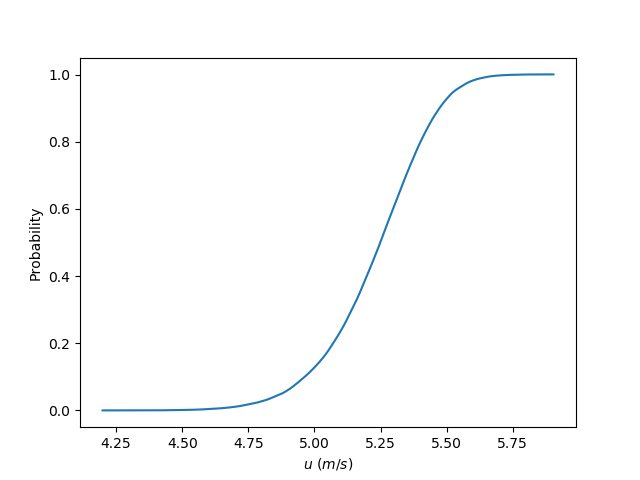
\includegraphics[width=0.6\linewidth]{Python/CDF_cl.png}
    \caption{Cumulative distribution function (CDF) computed from data at centreline ($y=30$ \si{mm})}
    \label{fig:CDF_cl}
\end{figure}

\subsection{Comments on spectra}

The matching of curves from different locations at figure \ref{fig:F11_filtering_and_comparison}.b seems to agree with Kolmogorov's predictions on universal laws of turbulence at small scales. The three one dimensional spectra fits very properly the one with the other after being made dimensionless using $\kappa^* = \kappa \eta$ and $F_{11}^*$ from $F_{11}$ using viscosity and dissipation rate. Concerning three dimensional spectra $E$ made dimensionless at figure \ref{fig:F_comparison}, the many operations to obtain it may have altered a bit the signal. Nevertheless, there is a range for $\kappa \gtrsim 7e-2$ where the three spectra match pretty well. That being said, the slope in this range seems to be slightly greater (in absolute value) than the $-5/3$ Kolmogorov's prediction.

\section{Error Analysis}

\section{Conclusions}

\newpage
% References
\bibliographystyle{apalike}
\bibliography{references}
\end{document}
